\documentclass[a4paper]{article}
\usepackage{graphicx}

\usepackage[  margin=2.5cm,  includefoot,  footskip=30pt,]{geometry}
\usepackage{pdflscape}
%\usepackage[cm]{fullpage}
\usepackage{bm}
\usepackage{listings}
\usepackage{amsmath}
\usepackage{amsfonts}
\usepackage{hyperref}
%\usepackage{xcolor}
\usepackage{mdframed}
\usepackage{makeidx} 
\usepackage{xargs}
\usepackage{upgreek}
\usepackage{algorithm,algorithmic}
\usepackage[pdftex,dvipsnames]{xcolor}
\usepackage[colorinlistoftodos,prependcaption,textsize=tiny]{todonotes}
\usepackage{amsthm}
\usepackage{gensymb} %\degree
\usepackage{siunitx} %\si{XX}
\newcommand{\aspect}{{\textsc{Aspect}}}
\newtheorem*{remark}{Remark}

\hypersetup{
    colorlinks,
    citecolor=black,
    filecolor=black,
    linkcolor=black,
    urlcolor=black
}
\lstset{ 
  language=Python,
  backgroundcolor=\color{white},   % choose the background color; you must add \usepackage{color} or \usepackage{xcolor}; should come as last argument
  basicstyle=\footnotesize,        % the size of the fonts that are used for the code
  breakatwhitespace=false,         % sets if automatic breaks should only happen at whitespace
  breaklines=true,                 % sets automatic line breaking
  captionpos=b,                    % sets the caption-position to bottom
  frame=single,                    % adds a frame around the code
  keepspaces=true,                 % keeps spaces in text, useful for keeping indentation of code (possibly needs columns=flexible)
  keywordstyle=\color{blue},       % keyword style
}
\newcommand\norm[1]{\left\lVert#1\right\rVert}

\newcommand{\nn}{\nonumber}
\newcommand{\A}{{\mathbb{A}}}
\newcommand{\K}{{\mathbb{K}}}
\newcommand{\G}{{\mathbb{G}}}
\newcommand{\Z}{{\mathbb{Z}}}
\newcommand{\C}{{\mathbb{C}}}
\newcommand{\W}{{\mathbb{W}}}
\newcommand{\LLL}{{\mathbb{L}}}
\newcommand{\SSS}{{\mathbb{S}}}
\newcommand{\fieldstone}{{\bf fieldstone}}

\newcommandx{\unsure}[2][1=]{\todo[linecolor=red,backgroundcolor=red!25,bordercolor=red,#1]{#2}}
\newcommandx{\change}[2][1=]{\todo[linecolor=blue,backgroundcolor=blue!25,bordercolor=blue,#1]{#2}}
\newcommandx{\info}[2][1=]{\todo[linecolor=OliveGreen,backgroundcolor=OliveGreen!25,bordercolor=OliveGreen,#1]{#2}}
\newcommandx{\improvement}[2][1=]{\todo[inline,linecolor=Plum,backgroundcolor=Plum!15,bordercolor=Plum,#1]{#2}}
\newcommandx{\thiswillnotshow}[2][1=]{\todo[disable,#1]{#2}}

%%%%%%%%%%%%%%%%%%%%%%%%%%%%%%%%%%%%%%%%%%%%%%%%%%%%%%%%%%%%%%%%%%%%%%%%%%%%%%%%%%%%%%%%%%%%%%%%%%%
%%%%%%%%%%%%%%%%%%%%%%%%%%%%%%%%%%%%%%%%%%%%%%%%%%%%%%%%%%%%%%%%%%%%%%%%%%%%%%%%%%%%%%%%%%%%%%%%%%%
%%%%%%%%%%%%%%%%%%%%%%%%%%%%%%%%%%%%%%%%%%%%%%%%%%%%%%%%%%%%%%%%%%%%%%%%%%%%%%%%%%%%%%%%%%%%%%%%%%%
%%%%%%%%%%%%%%%%%%%%%%%%%%%%%%%%%%%%%%%%%%%%%%%%%%%%%%%%%%%%%%%%%%%%%%%%%%%%%%%%%%%%%%%%%%%%%%%%%%%
%%%%%%%%%%%%%%%%%%%%%%%%%%%%%%%%%%%%%%%%%%%%%%%%%%%%%%%%%%%%%%%%%%%%%%%%%%%%%%%%%%%%%%%%%%%%%%%%%%%

\title{The Finite Element Method in Geodynamics}

\author{C. Thieulot}

\makeindex 
\begin{document}

\maketitle

\tableofcontents

\newpage

\begin{center}
{\color{red} \huge WARNING: this is work in progress}
\end{center}

%%%%%%%%%%%%%%%%%%%%%%
\section{Introduction}

\subsection{Philosophy} %------------------------------------------------------
This document was writing with my students in mind, i.e. 3rd and 4th year 
Geology/Geophysics students at Utrecht University. 
I have chosen to use as little jargon as possible unless it is a term that is 
commonly found in the geodynamics literature (methods paper as well as 
application papers). There is no mathematical proof of any theorem or statement 
I make. These are to be found in generic Numerical Analysic, Finite Element and 
Linear Algebra books. If you find that this books lacks references
to Sobolev spaces, Hilbert spaces, and other spaces, this book is just not for you.  

The codes I provide here are by no means optimised as I value code readability 
over code efficiency. I have also chosen to avoid resorting to multiple code 
files or even functions to favour a sequential reading of the codes. 
These codes are not designed to form the basis of a real life application:
Existing open source highly optimised codes shoud be preferred, such as 
ASPECT \cite{krhb12,hedg17}, CITCOM, LAMEM, PTATIN, PYLITH, ... 

All kinds of feedback is welcome on the text (grammar, typos, ...) or on the 
code(s). You will have my eternal gratitude if you wish to contribute an 
example, a benchmark, a cookbook. 

All the python scripts and this document are freely available at 
\begin{center}
\url{https://github.com/cedrict/fieldstone}
\end{center}

\subsection{Acknowledgments} %-------------------------------------------------

I have benefitted from many discussions, lectures, tutorials, coffee machine 
discussions, debugging sessions, conference poster sessions, etc ... 
over the years. I wish to name these instrumental people in particular and 
in alphabetic order: 
Wolfgang Bangerth, 
Jean Braun, 
Rens Elbertsen,
Philippe Fullsack, 
Menno Fraters, 
Anne Glerum,
Timo Heister,
Robert Myhill,
John Naliboff,
E. Gerry Puckett,
Melchior Schuh-Senlis,
Lukas van de Wiel,
Arie van den Berg, 
Tom Weir,
and the whole ASPECT family/team. 

%I wish to acknowledge many BSc and MSc students for their questions and feedback.
%and wish to mention: Job Mos (the
%very first version of fieldstone was part of his MSc thesis), 
%Tom Weir (contributions to the compressible formulation - MSc thesis), 
%and Rens Elbertsen (Tosi benchmark - BSc thesis).


\subsection{Essential literature} %--------------------------------------------

\begin{center}
\includegraphics[height=3.74cm]{images/literature/gerya_book}
\includegraphics[height=3.74cm]{images/literature/tackley_book}
\includegraphics[height=3.74cm]{images/literature/donea_huerta_book}
\includegraphics[height=3.74cm]{images/literature/bercovici_book}
\includegraphics[height=3.74cm]{images/literature/sto_book}\\
\end{center}

http://www-udc.ig.utexas.edu/external/becker/Geodynamics557.pdf

%---------------------------------------
\subsection{Installation}

If numpy, scipy or matplotlib are not installed on your machine, here is how you 
can install them:
\begin{verbatim}
python3.6 -m pip install --user numpy scipy matplotlib
\end{verbatim}
To install the umfpack solver:
\begin{verbatim}
pip install --upgrade scikit-umfpack --user
\end{verbatim}


\subsection{What is a fieldstone?} %-------------------------------------------
Simply put, it is stone collected from the surface of fields where it 
occurs naturally. It also stands for the bad acronym: {\sl fi}nite 
{\sl el}ement {\sl d}eformation of {\sl stone}s which echoes the primary 
application of these codes: geodynamic modelling.

\subsection{Why the Finite Element method?} \begin{flushright} {\tiny {\color{gray} why.tex}} \end{flushright}

The Finite Element Method (FEM) is by no means the only method 
to solve PDEs in geodynamics, nor it is necessarily always the best one.
Other methods are employed very successfully, such as the Finite Difference 
Method (FDM), the Finite Volume Method (FVM), and to a lesser extent
the Discrete Element Method (DEM) \cite{tasy05,egho07,egsc07,funi14}, 
the Lattice-Boltzmann method \cite{hupc08}, the Rigid Element Method \cite{lacj15},  
or the Element Free Galerkin Method (EFGM) \cite{hans03}.
I have been using FEM since 2008 and I do not have real 
experience to speak of in FVM or FDM (except for chapter 11)
so I concentrate in this book 
on what I know best. 


 %----------------------
\subsection{Notations} Scalars such as temperature, density, pressure, etc ... are simply 
obtained in \LaTeX{} by using the math mode, e.g. $T$, $\rho$, $p$.
Although it is common to lump vectors and matrices/tensors together
by using bold fonts, I have decided in the interest of clarity to 
distinguish between those: vectors are denoted by an arrow 
atop the quantity, e.g. $\vec \upnu$, $\vec g$, while matrices 
and tensors are in bold $\bm M$, $\bm \sigma$, etc ...

Also I use the $\cdot$ notation between two vectors to denote a 
dot product $\vec u \cdot \vec v = u_iv_i$ or a matrix-vector
multiplication ${\bm M}\cdot \vec a = M_{ij}a_j$. If there is no
$\cdot$ between vectors, it means that the result 
$\vec a \vec b = a_ib_j$ is a matrix (it is a dyadic 
product\footnote{\url{https://en.wikipedia.org/wiki/Dyadics}}.
Case in point, $\vec\nabla\cdot\vec\upnu$ is the velocity divergence
while $\vec\nabla\vec\upnu$ is the velocity gradient tensor.
 %-------------------------------------
\subsection{Colour maps for visualisation} \begin{flushright} {\tiny {\color{gray} colorscale.tex}} \end{flushright}

In an attempt to homogenise the figures obtained with ParaView, I have decided to use 
a fixed colour scale for each field throughout this document. These colour scales were 
obtained from \url{https://peterkovesi.com/projects/colourmaps} and are 
Perceptually Uniform Colour Maps \cite{kove15}. 

\begin{center}
\begin{tabular}{lll}
\hline
Field & colour code & \\
\hline\hline
Velocity/displacement & CET-D01A & \includegraphics[width=3cm]{images/colourscales/CET-D1A}\\
\hline
Pressure& CET-L17 & \includegraphics[width=3cm]{images/colourscales/CET-L17}\\
\hline
Velocity divergence& CET-L01 & \includegraphics[width=3cm]{images/colourscales/CET-L1}\\
\hline
Density& CET-D03 & \includegraphics[width=3cm]{images/colourscales/CET-D3}\\
\hline
Strain rate& CET-R2 & \includegraphics[width=3cm]{images/colourscales/CET-R2}\\
\hline
Viscosity & CET-R3 & \includegraphics[width=3cm]{images/colourscales/CET-R3}\\
\hline
Temperature & CET-D09 & \includegraphics[width=3cm]{images/colourscales/CET-D9}\\
\hline
stress & CET-L18 &  \includegraphics[width=3cm]{images/colourscales/CET-L18}\\
\hline
Spin tensor & CET-R1 &  \includegraphics[width=3cm]{images/colourscales/CET-R1}\\
\hline
Composition field & CET-CBD1 & \includegraphics[width=3cm]{images/colourscales/CET-CBD1}\\
\hline
Gravity acceleration & vik &  \includegraphics[width=3cm,height=7mm]{images/colourscales/vik}\\
\hline
Gravity potential & roma &  \includegraphics[width=3cm,height=7mm]{images/colourscales/roma}\\
\hline
\end{tabular}
\end{center}

vik and roma are available at \url{http://www.fabiocrameri.ch/colourmaps.php}.
See also Crameri \etal (2020) for a discussion about the misuse of 
colour is science communication.

%https://peterkovesi.com/projects/colourmaps/




 %----------------

%%%%%%%%%%%%%%%%%%%%%%%%%%%%%%%%%%%%%%%%%%%%%%%%%%%%%%%%%%%%%%%%%%%%%%%%%%%%%%%


{\small 

\noindent stone 01: simple analytical solution: "Donea \& Huerta" mms \ref{mms1} 
\lstinputlisting[language=bash,basicstyle=\tiny]{python_codes/fieldstone_01/keywords}

\noindent stone 02: Stokes sphere in 2D 
\lstinputlisting[language=bash,basicstyle=\tiny]{python_codes/fieldstone_02/keywords}

\noindent stone 03: Convection in a 2D box: "Blankenbach" benchmark \cite{blbc89}
\lstinputlisting[language=bash,basicstyle=\tiny]{python_codes/fieldstone_03/keywords}

\noindent stone 04: The lid driven cavity
\lstinputlisting[language=bash,basicstyle=\tiny]{python_codes/fieldstone_04/keywords}

\noindent stone 08: The indentor (punch problem) 
\lstinputlisting[language=bash,basicstyle=\tiny]{python_codes/fieldstone_08/keywords}

\noindent stone 10: Stokes sphere (3D) - penalty
\lstinputlisting[language=bash,basicstyle=\tiny]{python_codes/fieldstone_10/keywords}

\noindent stone 11: Stokes sphere (3D) - mixed formulation
\lstinputlisting[language=bash,basicstyle=\tiny]{python_codes/fieldstone_11/keywords}

\noindent stone 17: Solving the full saddle point problem in 3D - Burstedde benchmark \cite{dobo04} 
\lstinputlisting[language=bash,basicstyle=\tiny]{python_codes/fieldstone_17/keywords}

\noindent stone 18: Solving the full saddle point problem with $Q_2\times Q_1$ elements 
\lstinputlisting[language=bash,basicstyle=\tiny]{python_codes/fieldstone_18/keywords}

\noindent stone 19: Solving the full saddle point problem with $Q_3\times Q_2$ elements 
\lstinputlisting[language=bash,basicstyle=\tiny]{python_codes/fieldstone_19/keywords}

\noindent stone 20: Convection in a 3D box, the Busse benchmark \cite{bucc93}
\lstinputlisting[language=bash,basicstyle=\tiny]{python_codes/fieldstone_20/keywords}

\noindent stone 22: The stabilised $Q_1 \times Q_1$ element 
\lstinputlisting[language=bash,basicstyle=\tiny]{python_codes/fieldstone_22/keywords}

\noindent stone 25: Rayleigh-Taylor instability (1) - instantaneous \cite{vaks97}
\lstinputlisting[language=bash,basicstyle=\tiny]{python_codes/fieldstone_25/keywords}

\noindent stone 28: convection 2D box - Tosi et al, 2015
\lstinputlisting[language=bash,basicstyle=\tiny]{python_codes/fieldstone_28/keywords}

\noindent stone 33: Convection in an annulus 
\lstinputlisting[language=bash,basicstyle=\tiny]{python_codes/fieldstone_33/keywords}

\noindent stone 44: Flat slab setup 
\lstinputlisting[language=bash,basicstyle=\tiny]{python_codes/fieldstone_44/keywords}

\noindent stone 48: $Q_1\times P_0$, $Q_2\times Q_1$, $Q_3\times Q_2$ and $Q_4\times Q_3$ elements
\lstinputlisting[language=bash,basicstyle=\tiny]{python_codes/fieldstone_48/keywords}

\noindent stone 51: Triangular domain benchmark with MINI element
\lstinputlisting[language=bash,basicstyle=\tiny]{python_codes/fieldstone_51/keywords}

\noindent stone 58: Elastic disk under compression
\lstinputlisting[language=bash,basicstyle=\tiny]{python_codes/fieldstone_58/keywords}

\noindent stone 63: Failure in cemented granular material
\lstinputlisting[language=bash,basicstyle=\tiny]{python_codes/fieldstone_63/keywords}

\noindent stone 67: Newtonian subduction setups \& Particle-in-cell
\lstinputlisting[language=bash,basicstyle=\tiny]{python_codes/fieldstone_67/keywords}

\noindent stone 68: subduction \& corner flow
\lstinputlisting[language=bash,basicstyle=\tiny]{python_codes/fieldstone_68/keywords}

\noindent stone 69: Spherical shell 
\lstinputlisting[language=bash,basicstyle=\tiny]{python_codes/fieldstone_69/keywords}

}









 %%%%%%%%%%%%%%%%%%%%%%%%%%%%%%%%%%%%%%%%%%%%%%%%%%%%%%%%%%%%%%%%%%
%%%%%%%%%%%%%%%%%%%%%%%%%%%%%%%%%%%%%%%%%%%%%%%%%%%%%%%%%%%%%%%%%%%%%%%%%%%%%%%

\newpage
%%%%%%%%%%%%%%%%%%%%%%%%%%%%%%%%%%%%%%%%%%%%%%%%%%%%%%%%%%%%%%%%%%%%%%%%%%%%%%%
\section{The physical equations} %%%%%%%%%%%%%%%%%%%%%%%%%%%%%%%%%%%%%%%%%%%%%%

\begin{center}
\begin{tabular}{lll}
\hline
Symbol & meaning & unit \\
\hline
\hline
$t$ & Time & s \\
$x,y,z$ & Cartesian coordinates & m \\
${\bm v}$ & velocity vector & m$\cdot$ s$^{-1}$\\
$\rho$ & mass density & kg/m$^3$ \\
$\eta$ & dynamic viscosity &  Pa$\cdot$ s \\
$\lambda$ & penalty parameter & Pa$\cdot$ s \\
$T$ & temperature & K \\
${\bm \nabla}$ & gradient operator & m$^{-1}$ \\
${\bm \nabla}\cdot$ & divergence operator & m$^{-1}$ \\
$p$ & pressure & Pa\\
$\dot{\bm \varepsilon}({\bm v})$ & strain rate tensor & s$^{-1}$ \\
$\alpha$ & thermal expansion coefficient & K$^{-1}$ \\
$k$ & thermal conductivity & W/(m $\cdot$ K) \\
$C_p$ & Heat capacity & J/K \\
$H$ & intrinsic specific heat production & W/kg\\
$\beta_T$ & isothermal compressibility & Pa$^{-1}$  \\
${\bm \tau}$ & deviatoric stress tensor & Pa \\
${\bm \sigma}$ & full stress tensor & Pa \\
\hline
\end{tabular}
\end{center}

%------------------------------------------------------------------------
\subsection{The heat transport equation - energy conservation equation}

Let us start from the heat transport equation as shown in Schubert, Turcotte and Olson \cite{scto01}:
\[
\rho C_p \frac{DT}{Dt} - \alpha T \frac{Dp}{Dt} = {\bm \nabla} \cdot k {\bm \nabla} T + \Phi + \rho H  
\]
with $D/Dt$ being the total derivatives so that 
\[
\frac{DT}{Dt} = \frac{\partial T}{\partial t} + {\bm v}\cdot {\bm \nabla}T
\quad\quad
\frac{Dp}{Dt} = \frac{\partial p}{\partial t} + {\bm v}\cdot {\bm \nabla}p
\]
Solving for temperature, this equation is often rewritten as follows:
\begin{mdframed}[backgroundcolor=blue!5]
\[
\rho C_p \frac{DT}{Dt} - {\bm \nabla} \cdot k {\bm \nabla} T =  \alpha T \frac{Dp}{Dt} + \Phi + \rho H  
\]
\end{mdframed}

A note on the shear heating term $\Phi$: In many publications, $\Phi$ 
is given by $\Phi=\tau_{ij}\partial_j u_i={\bm \tau}:{\bm \nabla}{\bm v}$.

\begin{eqnarray}
\Phi 
&=& \tau_{ij}\partial_j u_i \nonumber\\
&=& 2 \eta \dot{\varepsilon}_{ij}^d\partial_j u_i \nonumber\\
&=& 2 \eta \frac{1}{2}\left( \dot{\varepsilon}_{ij}^d\partial_j u_i + \dot{\varepsilon}_{ji}^d\partial_i u_j \right) \nonumber\\
&=& 2 \eta \frac{1}{2}\left( \dot{\varepsilon}_{ij}^d\partial_j u_i + \dot{\varepsilon}_{ij}^d\partial_i u_j \right) \nonumber\\
&=& 2 \eta  \dot{\varepsilon}_{ij}^d  \frac{1}{2}\left(\partial_j u_i + \partial_i u_j \right) \nonumber\\
&=& 2 \eta  \dot{\varepsilon}_{ij}^d   \dot{\varepsilon}_{ij} \nonumber\\
&=& 2 \eta  \dot{\bm \varepsilon}^d :  \dot{\bm \varepsilon} \nonumber\\
&=& 2 \eta  \dot{\bm \varepsilon}^d : \left( \dot{\bm \varepsilon}^d +\frac{1}{3} ({\bm \nabla}\cdot{\bm v}) {\bm 1} \right)\nonumber\\
&=& 2 \eta  \dot{\bm \varepsilon}^d : \dot{\bm \varepsilon}^d 
+ 2 \eta  \dot{\bm \varepsilon}^d : {\bm 1} ({\bm \nabla}\cdot{\bm v}) \nonumber\\ 
&=& 2 \eta  \dot{\bm \varepsilon}^d : \dot{\bm \varepsilon}^d 
\end{eqnarray}
Finally
\[
\Phi = {\bm \tau}:{\bm \nabla}{\bm v} = 2 \eta  \dot{\bm \varepsilon}^d : \dot{\bm \varepsilon}^d
= 2 \eta \left( (\dot{\varepsilon}_{xx}^d)^2 + (\dot{\varepsilon}_{yy}^d)^2 + 2(\dot{\varepsilon}_{xy}^d)^2 \right)
\]

%------------------------------------------------------------------------
\subsection{The momentum conservation equations} 

Because the Prandlt number is virtually zero in Earth science applications the Navier Stokes 
equations reduce to the Stokes equation:
\[
{\bm \nabla}\cdot {\bm \sigma} + \rho {\bm g} = 0
\]
Since 
\[
{\bm \sigma} = -p {\bm 1} + {\bm \tau}
\]
it also writes
\[
-{\bm \nabla}p + {\bm \nabla}\cdot {\bm \tau} + \rho {\bm g} = 0
\]
Using the relationship ${\bm \tau} = 2 \eta \dot{\bm \varepsilon}^d$ we arrive at 
\begin{mdframed}[backgroundcolor=blue!5]
\[
-{\bm \nabla}p + {\bm \nabla}\cdot (2 \eta \dot{\bm \varepsilon}^d ) + \rho {\bm g} = 0
\]
\end{mdframed}

%------------------------------------------------------------------------
\subsection{The mass conservation equations} 

The mass conservation equation is given by
\[
\frac{D\rho}{Dt} + \rho {\bm \nabla}\cdot{\bm v} = 0
\]
or, 
\begin{mdframed}[backgroundcolor=blue!5]
\[
\frac{\partial \rho}{\partial t} + {\bm \nabla}\cdot(\rho {\bm v}) = 0
\]
\end{mdframed}
In the case of an incompressible flow, then $\partial \rho/\partial t=0$ and 
${\bm \nabla}\rho=0$, i.e. $D\rho/Dt=0$ and the remaining equation is simply:
\[
{\bm \nabla}\cdot{\bm v} = 0
\]

\subsection{The equations in ASPECT manual}
The following is lifted off the ASPECT manual.
We focus on the system of equations in a $d=2$- or $d=3$-dimensional
domain $\Omega$ that describes the motion of a highly viscous fluid driven
by differences in the gravitational force due to a density that depends on
the temperature. In the following, we largely follow the exposition of this
material in Schubert, Turcotte and Olson \cite{scto01}.

Specifically, we consider the following set of equations for velocity $\mathbf
u$, pressure $p$ and temperature $T$:
\begin{align}
  \label{eq:stokes-1}
  -\nabla \cdot \left[2\eta \left(\dot\varepsilon(\bm v)
                                  - \frac{1}{3}(\nabla \cdot \bm v)\mathbf 1\right)
                \right] + \nabla p &=
  \rho \bm g
  &
  & \textrm{in $\Omega$},
  \\
  \label{eq:stokes-2}
  \nabla \cdot (\rho \bm v) &= 0
  &
  & \textrm{in $\Omega$},
  \\
  \label{eq:temperature}
  \rho C_p \left(\frac{\partial T}{\partial t} + \bm v\cdot\nabla T\right)
  - \nabla\cdot k\nabla T
  &=
  \rho H
  \notag
  \\
  &\quad
  +
  2\eta
  \left(\dot\varepsilon(\bm v) - \frac{1}{3}(\nabla \cdot \bm v)\mathbf 1\right)
  :
  \left(\dot\varepsilon(\bm v) - \frac{1}{3}(\nabla \cdot \bm v)\mathbf 1\right)
  \\
  &\quad
  +\alpha T \left( \bm v \cdot \nabla p \right)
  \notag
  \\
  &\quad
  &
  & \textrm{in $\Omega$},
  \notag
\end{align}
where $\dot{\bm \varepsilon}(\mathbf u) = \frac{1}{2}(\nabla \mathbf u + \nabla\mathbf
u^T)$ is the symmetric gradient of the velocity (often called the
\textit{strain rate}).%

In this set of equations, \eqref{eq:stokes-1} and \eqref{eq:stokes-2}
represent the compressible Stokes equations in which $\mathbf v=\mathbf
v(\mathbf x,t)$ is the velocity field and $p=p(\mathbf x,t)$ the pressure
field. Both fields depend on space $\mathbf x$ and time $t$. Fluid flow is
driven by the gravity force that acts on the fluid and that is proportional to
both the density of the fluid and the strength of the gravitational pull.

Coupled to this Stokes system is equation \eqref{eq:temperature} for the
temperature field $T=T(\mathbf x,t)$ that contains heat conduction terms as
well as advection with the flow velocity $\mathbf v$. The right hand side
terms of this equation correspond to
\begin{itemize}
\item internal heat production for example due to radioactive decay;
\item friction (shear) heating;
\item adiabatic compression of material;
\end{itemize}

In order to arrive at the set of equations that ASPECT solves, 
we need to 
\begin{itemize}
\item neglect the $\partial p/\partial t$. {\color{red}WHY?}
\item neglect the $\partial \rho / \partial t$ . {\color{red}WHY?}
\end{itemize}
from equations above. 

----------------------------------------

Also, their definition of the shear heating term $\Phi$ is:
\[
\Phi = k_B ({\bm \nabla}\cdot{\bm v})^2 + 2\eta \dot{\bm \varepsilon}^d:\dot{\bm \varepsilon}^d
\]
For many fluids the bulk viscosity $k_B$ is very small and is often taken to be zero, an assumption known
as the Stokes assumption: $k_B=\lambda+2\eta/3=0$. \index{bulk viscosity}
Note that $\eta$ is the dynamic viscosity and $\lambda$ the second viscosity. \index{dynamic viscosity}
\index{second viscosity}
Also, 
\[
{\bm \tau}=2\eta \dot{\bm \varepsilon} + \lambda ({\bm \nabla}\cdot{\bm v}) {\bm 1}
\]
but since $k_B=\lambda+2\eta/3=0$, then $\lambda=-2\eta/3$ so 
\[
{\bm \tau}=2\eta \dot{\bm \varepsilon} -\frac{2}{3}\eta ({\bm \nabla}\cdot{\bm v}) {\bm 1} = 2\eta \dot{\bm \varepsilon}^d
\]







\newpage
%---------------------------------
\subsection{the Boussinesq approximation: an Incompressible flow}

\index{Boussinesq}

[from aspect manual]
The Boussinesq approximation assumes that the density can be
considered constant in all occurrences in the equations with the exception of
the buoyancy term on the right hand side of \eqref{eq:stokes-1}. The primary
result of this assumption is that the continuity equation \eqref{eq:stokes-2}
will now read
\[
{\bm \nabla}\cdot{\bm v} = 0
\]
This implies that the strain rate tensor is deviatoric.
Under the Boussinesq approximation, the equations are much simplified:

\begin{align}
  \label{eq:stokes-1}
  -\nabla \cdot \left[2\eta \dot{\bm \varepsilon}(\bm v)
                \right] + \nabla p &=
  \rho \bm g
  &
  & \textrm{in $\Omega$},
  \\
  \label{eq:stokes-2}
  \nabla \cdot (\rho \bm v) &= 0
  &
  & \textrm{in $\Omega$},
  \\
  \label{eq:temperature}
  \rho_0 C_p \left(\frac{\partial T}{\partial t} + \bm v\cdot\nabla T\right)
  - \nabla\cdot k\nabla T
  &=
  \rho H
  &
  & \textrm{in $\Omega$}
\end{align}
Note that all terms on the rhs of the temperature equations have disappeared, with the exception 
of the source term.


\newpage
\subsection{Stokes equation for elastic medium}

What follows is mostly borrowed from Becker \& Kaus lecture notes.

%\begin{tabular}{|l|l|l|}
%\hline
%${\bm u}       $ & displacement vector &   \\
%${\bm \sigma}  $ & full stress tensor  & Pa\\
%${\bm \epsilon}$ & strain tensor       &   \\
%${\bm 1}       $ & unit tensor         &   \\
%${\bm f}       $ & body forces         &   \\
%\hline
%\end{tabular}

The strong form of the PDE that governs force balance in a medium is given by
\[
{\bm \nabla}\cdot{\bm \sigma}  + {\bm f} = {\bm 0}
\]
where ${\bm \sigma}$ is the stress tensor and ${\bm f}$ is a body force.

The stress tensor is related to the strain tensor through the generalised 
Hooke's law:
\begin{equation}
\sigma_{ij}=\sum_{kl}C_{ijkl}\epsilon{kl} \label{eq:one}
\end{equation}
where ${\bm C}$ is the fourth-order elastic tensor.
In the case of an isotropic material, this relationship simplifies to
\begin{equation}
\sigma_{ij}=\lambda \epsilon_{kk} \delta_{ij} + 2\mu \epsilon_{ij}
\quad\quad
or, 
\quad\quad
{\bm \sigma} = \lambda ({\bm \nabla}\cdot{\bm u})  {\bm 1} + 2\mu {\bm \epsilon}   \label{eq:two}
\end{equation}
where $\lambda$ is the Lam\'e parameter and $\mu$ is the shear modulus\footnote{It is also sometimes written $G$}.
The term ${\bm \nabla}\cdot{\bm u}$ is the isotropic dilation.

\index{Lam\'e parameter} \index{shear modulus}

The strain tensor is related to the displacement as follows: \index{strain tensor}
\[
{\bm \epsilon} = \frac{1}{2}({\bm \nabla}{\bm u} + {\bm \nabla}{\bm u}^T)
\]

The incompressibility (bulk modulus), $K$, is defined as $p=-K {\bm \nabla}\cdot{\bm u}$ 
where $p$ is the pressure with \index{bulk modulus}
\begin{eqnarray}
p&=&-\frac{1}{3}Tr({\bm \sigma}) \nonumber\\
 &=& -\frac{1}{3} [ \lambda ({\bm \nabla}\cdot{\bm u}) Tr[{\bm 1}] + 2 \mu Tr[{\bm \epsilon}]] \nonumber\\
 &=& -\frac{1}{3} [ \lambda ({\bm \nabla}\cdot{\bm u})  3  + 2 \mu  ({\bm \nabla}\cdot{\bm u}) ] \nonumber\\
 &=& -[ \lambda  + \frac{2}{3} \mu ]   ({\bm \nabla}\cdot{\bm u})  
\end{eqnarray}
so that $K=\lambda+\frac{2}{3}\mu$.

%or
%\[
%\mu=\frac{3K(1-2\nu)}{2(1+\nu)}
%\]


\paragraph{Remark}: Eq. (\ref{eq:one}) and (\ref{eq:two}) are analogous to the ones that one has to solve
in the context of viscous flow using the penalty method. In this case $\lambda$ is the penalty coefficient, 
${\bm u}$ is the velocity, and $\mu$ is then the dynamic viscosity.

%\begin{center}
%\includegraphics[width=15cm]{images/coeffs}\\
%{\small Homogeneous isotropic linear elastic materials have their elastic properties uniquely determined by any two moduli among these; thus, given any two, any other of the elastic moduli can be calculated according to these formulas.}
%\end{center}

The Lam\'e parameter and the shear modulus are also linked to $\nu$ the poisson ratio, 
and $E$, Young's modulus: \index{Poisson ratio} \index{Young's modulus}
\[
\lambda=\mu\frac{2\nu}{1-2\nu}
=\frac{\nu E}{(1+\nu)(1-2\nu)}
\quad\quad
{\rm with}
\quad\quad
E=2\mu(1+\nu)
\]
The shear modulus, expressed often in GPa, describes the material's response to shear stress.
The poisson ratio describes the response in the direction orthogonal to uniaxial stress.
The Young modulus, expressed in GPa, describes the material's strain response to uniaxial stress in the 
direction of this stress.









 %%%%%%%%%%%%%%%%%%%%%%%%%%%%%%%%%%%%%%%%%%%%%%%%%%%%%%%%%%%%%%%
%%%%%%%%%%%%%%%%%%%%%%%%%%%%%%%%%%%%%%%%%%%%%%%%%%%%%%%%%%%%%%%%%%%%%%%%%%%%%%%

\newpage
%%%%%%%%%%%%%%%%%%%%%%%%%%%%%%%%%%%%%%%%%%%%%%%%%%%%%%%%%%%%%%%%%%%%%%%%%%%%%%%%%%%%%%%%%%%%%%%%%%%
\section{The building blocks of the Finite Element Method} %%%%%%%%%%%%%%%%%%%%%%%%%%%%%%%%%%%%%%%%
\subsection{Numerical integration} As we will see later, using the Finite Element method to solve problems involves computing integrals which are more often than not too complex to be computed analytically/exactly. We will then need to compute them numerically.

[wiki] In essence, 
the basic problem in numerical integration is to compute an approximate solution to a definite integral
\[
\int_a^b f(x) dx
\]
to a given degree of accuracy.
This problem has been widely studied and we know that 
if $f(x)$ is a smooth function, and the domain of integration is bounded, there are many methods for approximating the integral to the desired precision.

There are several reasons for carrying out numerical integration.
\begin{itemize}
\item The integrand $f(x)$ may be known only at certain points, such as obtained by sampling. Some embedded systems and other computer applications may need numerical integration for this reason.
\item A formula for the integrand may be known, but it may be difficult or impossible to find an antiderivative that is an elementary function. An example of such an integrand is $f(x)=exp(-x^2)$, the antiderivative of which (the error function, times a constant) cannot be written in elementary form.
\item It may be possible to find an antiderivative symbolically, but it may be easier to compute a numerical approximation than to compute the antiderivative. That may be the case if the antiderivative is given as an infinite series or product, or if its evaluation requires a special function that is not available.
\end{itemize}

%-----------------------------
\subsubsection{in 1D - theory}

The simplest method of this type is to let the interpolating function be a constant function (a polynomial of degree zero) that passes through the point $((a+b)/2, f((a+b)/2))$.

This is called the midpoint rule \index{midpoint rule} or rectangle rule. \index{rectangle rule}
\[
\int_a^b f(x)dx \simeq (b-a) f(\frac{a+b}{2})
\]

\improvement[inline]{insert here figure}

The interpolating function may be a straight line (an affine function, i.e. a polynomial of degree 1)
passing through the points $(a, f(a))$ and $(b, f(b))$.

This is called the trapezoidal rule. \index{trapezoidal rule} 
\[
\int_a^b f(x)dx \simeq (b-a) \frac{f(a)+f(b)}{2}
\]

\improvement[inline]{insert here figure}

For either one of these rules, we can make a more accurate approximation by breaking up the interval [a, b] into some number n of subintervals, computing an approximation for each subinterval, then adding up all the results. This is called a composite rule, extended rule, or iterated rule. For example, the composite trapezoidal rule can be stated as

\[
\int_a^b f(x)dx \simeq \frac{b-a}{n} \left( \frac{f(a)}{2}  
+\sum_{k=1}^{n-1} f(a+k\frac{b-a}{n})
   +\frac{f(b)}{2} \right)
\]

where the subintervals have the form $[kh,(k+1)h]$, with $h=(b-a)/n$ and $k=0,1,2,\dots,n-1$.


\begin{center}
a)\includegraphics[width=7cm]{images/quadrature/int1}
b)\includegraphics[width=7cm]{images/quadrature/int2}\\
The interval $[-2,2]$ is broken into 16 sub-intervals. The blue lines correspond to the 
approximation of the red curve by means of a) the midpoint rule,  b) the trapezoidal rule.
\end{center}

There are several algorithms for numerical integration (also commonly called 'numerical quadrature', or
simply 'quadrature') \index{quadrature}.
Interpolation with polynomials evaluated at equally spaced points in $[a,b]$
yields the Newton–Cotes formulas, of which the rectangle rule and the trapezoidal rule are examples. \index{Newton-Cotes}
If we allow the intervals between interpolation points to vary, we find another group of quadrature formulas, such as 
the Gauss(ian) quadrature formulas. \index{Gauss quadrature}
A Gaussian quadrature rule is typically more accurate than a Newton–Cotes rule, 
which requires the same number of function evaluations, if the integrand is smooth 
(i.e., if it is sufficiently differentiable).


An $n-$point Gaussian quadrature rule, named after Carl Friedrich Gauss, is a quadrature rule constructed
to yield an exact result for polynomials of degree $2n-1$ or less by a suitable choice of the points $x_i$
and weights $w_i$ for $i=1,\dots,n$.

The domain of integration for such a rule is conventionally taken as $[-1,1]$, so the rule is stated as
\[
\int_{-1}^{+1} f(x) dx = \sum_{i_q=1}^n w_{i_q} f(x_{i_q})
\]
In this formula the $x_{i_q}$ coordinate is 
the $i$-th root of the Legendre polynomial $P_n(x)$. \index{Legendre polynomial}

It is important to note that a Gaussian quadrature will only produce good results if the function $f(x)$
is well approximated by a polynomial function within the range $[-1,1]$.
As a consequence, the method is not, for example, suitable for functions with singularities.

\begin{center}
\includegraphics[width=5.cm]{images/quadrature/gq2}\\
Gauss-Legendre points and their weights.
\end{center}

As shown in the above table, it can be shown that the weight values must fulfill the following condition:
\begin{equation}
\sum_{i_q} w_{i_q}=2 \label{gq23}
\end{equation}
and it is worth noting that all quadrature point coordinates are symmetrical around the origin.

Since most quadrature formula are only valid on a specific interval, we now must address the problem 
of their use outside of such intervals. The solution turns out to be quite simple: one 
must carry out a change of variables from the interval $[a,b]$ to $[-1,1]$.

We then consider the reduced coordinate $r\in[-1,1]$ such that 
\[
r=\frac{2}{b-a}(x-a)-1 
\]
This relationship can be reversed such that when $r$ is known, its equivalent coordinate 
$x\in[a,b]$ can be computed:
\[
x=\frac{b-a}{2}(1+r)+a
\]
From this it follows that
\[
dx=\frac{b-a}{2}dr
\]
and then 
\[
\int_a^b f(x) dx  = \frac{b-a}{2} \int_{-1}^{+1} f(r) dr \simeq 
\frac{b-a}{2} \sum_{i_q=1}^n w_{i_q} f(r_{i_q})
\]

%--------------------
\subsubsection{in 1D - examples}

\paragraph{example 1}

Since we know how to carry out any required change of variables, we choose for simplicity 
$a=-1$, $b=+1$.
Let us take for example $f(x)=\pi$. Then we can compute the integral of this function 
over the interval $[a,b]$ exactly:
\[
I=\int_{-1}^{+1} f(x) dx = \pi \int_{-1}^{+1}dx  = 2 \pi
\]
We can now use a Gauss-Legendre formula to compute this same integral:
\[
I_{gq}=\int_{-1}^{+1} f(x) dx 
= \sum_{i_q=1}^{n_q} w_{i_q} f(x_{i_q}) 
= \sum_{i_q=1}^{n_q} w_{i_q} \pi
= \pi \underbrace{\sum_{i_q=1}^{n_q} w_{i_q} }_{=2}
= 2 \pi
\]
where we have used the property of the weight values of Eq.(\ref{gq23}).
Since the actual number of points was never specified, this result is valid for all 
quadrature rules.


\paragraph{example 2}

Let us now take $f(x)=m x+ p$ and repeat the same exercise:
\[
I=\int_{-1}^{+1} f(x) dx = \int_{-1}^{+1} (mx+p) dx  =  [\frac{1}{2} m x^2 + p x ]_{-1}^{+1} =2p
\]
\[
I_{gq}=\int_{-1}^{+1} f(x) dx 
\!= \sum_{i_q=1}^{n_q} w_{i_q} f(x_{i_q}) 
\!= \sum_{i_q=1}^{n_q} w_{i_q} (m x_{i_q} + p)  
\!= m \underbrace{\sum_{i_q=1}^{n_q} w_{i_q} x_{i_q}}_{=0}  + p \underbrace{\sum_{i_q=1}^{n_q} w_{i_q}}_{=2}  = 2p
\]
since the quadrature points are symmetric w.r.t. to zero on the x-axis.
Once again the quadrature is able to compute the exact value of this integral: this makes sense since 
an $n$-point rule exactly integrates a $2n-1$ order polynomial such that a 1 point quadrature exactly 
integrates a first order polynomial like the one above.



\paragraph{example 3}

Let us now take $f(x)=x^2$. We have 
\[
I=\int_{-1}^{+1} f(x) dx = \int_{-1}^{+1} x^2 dx  =  [\frac{1}{3}x^3 ]_{-1}^{+1} =  \frac{2}{3} 
\]
and 
\[
I_{gq}=\int_{-1}^{+1} f(x) dx 
\!= \sum_{i_q=1}^{n_q} w_{i_q} f(x_{i_q}) 
\!= \sum_{i_q=1}^{n_q} w_{i_q} x_{i_q}^2 
\]

\begin{itemize}
\item $n_q=1$: $x_{iq}^{(1)}=0$, $w_{i_q}=2$. $I_{gq}=0$
\item $n_q=2$: $x_{q}^{(1)}=-1/\sqrt{3}$, $x_{q}^{(2)}=1/\sqrt{3}$, $w_{q}^{(1)}=w_{q}^{(2)}=1$. $I_{gq}=\frac{2}{3}$
\item It also works $\forall n_q>2$ !
\end{itemize}

%-----------------------------
\subsubsection{in 2D/3D - theory}


Let us now turn to a two-dimensional integral of the form
\[
I=\int_{-1}^{+1} \int_{-1}^{+1} f(x,y) dx dy
\]
The equivalent Gaussian quadrature writes:
\[
I_{gq}
\simeq \sum_{i_q=1}^{n_q}\sum_{j_q}^{n_q} f(x_{i_q},y_{j_q}) w_{i_q} w_{j_q}
\]


%----------------------------------------
\subsubsection{quadrature on tetrahedra}

Quadrature rules on tetrahedra take the form:
\[
\int\int\int_{el} f(x,y,z) dxdydz = V_{el} \sum_{iq=1}^{nqel} w_{iq} f(\xi^{iq}_1,\xi^{iq}_2,\xi^{iq}_3,\xi^{iq}_4) 
\]
or, that is to say:
\[
\int\int\int_{el} f(x,y,z) dxdydz = \sum_{iq=1}^{nqel} (w_{iq}V_{el}) f(\xi^{iq}_1,\xi^{iq}_2,\xi^{iq}_3,\xi^{iq}_4) 
\]
with in our case $V_{el}=1/6$.

In the literature it can be found that a one point quadrature is characterised by 
\[
w_{iq}=1 \quad\quad\quad \xi^{iq}_1=\xi^{iq}_2=\xi^{iq}_3=\xi^{iq}_4=0.25
\]
i.e, the coordinates of the single point are given by:
\[
x_{iq}=\sum_{i=1}^4 \xi_i^{iq} x_i = \frac{1}{4} (x_1+x_2+x_3+x_4)
\]
Same for $y$ and $z$ coordinates. 

A four-point quadrature rule is characterised by $w_{iq}=0.25$ and 

\begin{tabular}{lcccc}
 & $\xi_1$ & $\xi_2$ & $\xi_3$ & $\xi_4$ \\
iq=1 & 0.585410196624969 & 0.138196601125011 & 0.138196601125011 & 0.138196601125011 \\
iq=2 & 0.138196601125011 & 0.585410196624969 & 0.138196601125011 & 0.138196601125011 \\
iq=3 & 0.138196601125011 & 0.138196601125011 & 0.585410196624969 & 0.138196601125011 \\
iq=4 & 0.138196601125011 & 0.138196601125011 & 0.138196601125011 & 0.585410196624969 
\end{tabular}
We then have:
\[
r_{iq}=\sum_{i=1}^4 \xi_i^{iq} x_i 
= (\xi_1^{iq},\xi_2^{iq},\xi_3^{iq},\xi_4^{iq})\cdot(r_1,r_2,r_3,r_4) 
= (\xi_1^{iq},\xi_2^{iq},\xi_3^{iq},\xi_4^{iq})\cdot(0,1,0,0) 
= \xi_2^{iq}
\]
\[
s_{iq}=\sum_{i=1}^4 \xi_i^{iq} y_i 
= (\xi_1^{iq},\xi_2^{iq},\xi_3^{iq},\xi_4^{iq})\cdot(s_1,s_2,s_3,s_4) 
= (\xi_1^{iq},\xi_2^{iq},\xi_3^{iq},\xi_4^{iq})\cdot(0,0,1,0) 
= \xi_3^{iq}
\]
\[
t_{iq}=\sum_{i=1}^4 \xi_i^{iq} z_i 
= (\xi_1^{iq},\xi_2^{iq},\xi_3^{iq},\xi_4^{iq})\cdot(t_1,t_2,t_3,t_4) 
= (\xi_1^{iq},\xi_2^{iq},\xi_3^{iq},\xi_4^{iq})\cdot(0,0,0,1) 
= \xi_4^{iq}
\]
Finally:

\begin{tabular}{llll}
     & $r$ & $s$ & $t$ \\
iq=1 & 0.138196601125011 & 0.138196601125011 & 0.138196601125011\\
iq=2 & 0.585410196624969 & 0.138196601125011 & 0.138196601125011\\
iq=3 & 0.138196601125011 & 0.585410196624969 & 0.138196601125011\\
iq=4 & 0.138196601125011 & 0.138196601125011 & 0.585410196624969\\
\end{tabular}





 %--------------------------------------------
\subsection{The mesh}
\subsection{A bit of FE terminology} 
We introduce here some terminology for efficient element descriptions \cite{grsa}:
\begin{itemize}
\item For triangles/tetrahedra, the designation 
$P_m \times P_n$ \index{general}{$P_m \times P_n$}
means that each component of the velocity
is approximated by continuous piecewise \index{general}{Piecewise} complete Polynomials of degree $m$ and
pressure by continuous piecewise complete Polynomials of degree  $n$.
For example $P_2 \times P_1$ means 
\[
u \sim a_1 + a_2 x + a_3 y + a_4 xy + a_5 x^2 + a_6 y^2
\]
with similar approximations for $v$, and 
\[
p \sim b_1 + b_2x + b_3 y
\]
Both velocity and pressure are continuous across element boundaries, 
and each triangular element contains 6 velocity nodes and three pressure nodes.

\item For the same families, \index{general}{$P_m \times P_{-n}$} 
$P_m \times P_{-n}$
is as above, except that pressure is approximated via 
piecewise {\sl discontinuous} polynomials of degree $n$. For instance, $P_2 \times P_{-1}$ is the same 
as $P_2P_1$ except that pressure is now an independent linear function in each element and therefore 
discontinuous at element boundaries.

\item For quadrilaterals/hexahedra, the designation 
\index{general}{$Q_m \times Q_n$}  $Q_m \times Q_n$
means that each component of the velocity
is approximated by a continuous piecewise polynomial of degree $m$ {\sl in each direction} on the quadrilateral
and likewise for pressure, except that the polynomial is of degree $n$.
For instance,  $Q_2 \times Q_1$ \index{general}{$Q_2 \times Q_1$} means
\[
u \sim a_1 + a_2 x + a_3 y + a_4 xy + a_5 x^2 + a_6 y^2 + a_7 x^2y + a_8 xy^2 + a_9 x^2y^2
\]
and 
\[
p \sim b_1 + b_2x + b_3 y + b_4 xy
\]
\item For these same families, $Q_m \times Q_{-n}$ is as above, except that the pressure approximation 
is not continuous at element boundaries. \index{general}{$Q_m \times Q_{-n}$}

\item Again for the same families, \index{general}{$Q_m \times P_{-n}$} $Q_m \times P_{-n}$
 indicates the same velocity approximation 
with a pressure approximation that is a discontinuous complete piecewise polynomial of degree $n$
(not of degree $n$ in each direction !)

\item The designation $P_m^+$ or $Q_m^+$ means that some sort of bubble function \index{general}{Bubble Function}
was added to the polynomial approximation for the velocity. You may also find the term 'enriched element'
in the literature.

\item Finally, for $n=0$, we have piecewise-constant pressure, and we omit the minus sign for simplicity.
\end{itemize}

Another point which needs to be clarified is the use of so-called 'conforming elements' 
(or 'non-conforming elements'). \index{general}{Conforming Element} \index{general}{Non-Conforming Element}
Following again \cite{grsa}, conforming velocity elements are those for which the basis functions for a subset 
of $H^1$ for the continuous problem (the first derivatives and their squares are integrable in $\Omega$).
For instance, the rotated $Q_1 \times P_0$ element of Rannacher and Turek (see section \ref{pair}) is such that 
the velocity is discontinous across element edges, so that the derivative does not exist there. Another
typical example of non-conforming element is the Crouzeix-Raviart element \cite{crra73}.

 


 %-----------------------------------------
\subsection{Elements and basis functions in 1D} \begin{flushright} {\tiny {\color{gray} elements1D.tex}} \end{flushright}


%------------------------------------------
\subsection{Linear basis functions ($Q_1$) \label{sec:bf1}}
\index{general}{$Q_1$}

Let $f(r)$ be a $C^1$ function on the interval $[-1:1]$ with $f(-1)=f_1$  and $f(1)=f_2$.
\begin{center}
\includegraphics[width=8cm]{images/linshapefct.png}
\end{center}
Let us assume that the function $f(r)$ is to be approximated on $[-1,1]$ by the first order polynomial 
\begin{equation}
f^h(r)=a+br \label{eqquad1}
\end{equation}
Then it must fulfil
\begin{eqnarray}
f^h(r=-1)&=&a-b =f_1 \nonumber\\
f^h(r=+1)&=&a+b =f_2 \nonumber
\end{eqnarray}
This leads to  
\begin{eqnarray}
a&=&\frac{1}{2}(f_1+f_2)  \nn\\
b&=&\frac{1}{2}(-f_1+f_2)  
\end{eqnarray}
and then replacing $a,b$ in Eq.~\eqref{eqquad1} by the above values one gets
\[
f^h(r) = \left[  \frac{1}{2}(1-r)\right] f_1 + \left[ \frac{1}{2}(1+r) \right] f_2
\]
or
\[
f^h(r)=\sum_{i=1}^2 N_i(r) f_1
\]
with
\begin{mdframed}[backgroundcolor=blue!5]
\begin{eqnarray}
N_1(r) &=& \frac{1}{2} (1-r) \nonumber\\
N_2(r) &=& \frac{1}{2} (1+r)
\end{eqnarray}
\end{mdframed}

\begin{center}
\includegraphics[width=8cm]{images/basis1D/linear.pdf}\\
{\captionfont Plot of the two linear functions $N_1(r)$ and $N_2(r)$.}
\end{center}

\newpage
%------------------------------------------
\subsection{Quadratic basis functions ($Q_2$) \label{sec:bf2}}
\index{general}{$Q_2$}

Let $f(r)$ be a $C^1$ function on the interval $[-1:1]$ with $f(-1)=f_1$, $f(0)=f_2$ and $f(1)=f_3$.
\begin{center}
\includegraphics[width=8cm]{images/quadshapefct.png}
\end{center}
Let us assume that the function $f(r)$ is to be approximated on $[-1,1]$ by the second order polynomial 
$f^h(r)$:
\begin{equation}
f(r)=a+br+cr^2 \label{eqquad}
\end{equation}
Then it must fulfil
\begin{eqnarray}
f^h(r=-1)&=&a-b+c = f_1 \nonumber\\
f^h(r=0) &=&a\quad\quad\quad\;     = f_2 \nonumber\\
f^h(r=+1)&=&a+b+c = f_3 \nonumber
\end{eqnarray}
This leads to
\begin{eqnarray}
a&=&f_2   \nn\\
b&=&\frac{1}{2}(-f_1+f_3)  \nn\\
c&=&\frac{1}{2}(f_1+f_3-2f_2) 
\end{eqnarray}
and then replacing $a,b,c$ in Eq.~\eqref{eqquad} by the above values on gets
\[
f^h(r)=\left[\frac{1}{2}r(r-1)\right] f_1 + (1-r^2) f_2 + \left[\frac{1}{2}r(r+1)\right] f_3
\]
or,
\[
\boxed{
f^h(r) = \sum_{i=1}^3 N_i(r) f_i
}
\]
with
\begin{mdframed}[backgroundcolor=blue!5]
\begin{eqnarray}
N_1(r) &=& \frac{1}{2}r(r-1) \nonumber\\
N_2(r) &=& (1-r^2) \nonumber\\ 
N_3(r) &=& \frac{1}{2}r(r+1) 
\end{eqnarray}
\end{mdframed}

\begin{center}
\includegraphics[width=8cm]{images/basis1D/quadratic.pdf}\\
{\captionfont Plot of the three quadratic functions $N_1(r)$, $N_2(r)$ and $N_3(r)$.}
\end{center}
Note that $Q_2$ basis functions can take negative values. 

We will later need the first-order derivatives of these functions:
\begin{mdframed}[backgroundcolor=blue!5]
\begin{eqnarray}
\frac{\partial N_1}{\partial r} &=& r-\frac{1}{2} \nonumber\\
\frac{\partial N_2}{\partial r} &=& -2r \nonumber\\ 
\frac{\partial N_3}{\partial r} &=& r+\frac{1}{2}
\end{eqnarray}
\end{mdframed}


%------------------------------------------
\subsection{Cubic basis functions ($Q_3$) \label{sec:bf3}}
\index{general}{$Q_3$}

We proceed as previously by assuming that the third-order 
polynomial representation of function $f(r)$ is given by
\[
f^h(r)=a+br+cr^2+dr^3
\]
with the nodes at position -1,-1/3, +1/3 and +1.
It then must fulfil all four conditions:
\begin{eqnarray}
f(-1)   &=& a-b+c-d = f_1 \nonumber\\
f(-1/3) &=& a-\frac{b}{3}+\frac{c}{9}-\frac{d}{27} = f_2 \nonumber\\
f(+1/3) &=& a-\frac{b}{3}+\frac{c}{9}-\frac{d}{27} = f_3 \nonumber\\
f(+1)   &=& a+b+c+d = f_4 \nonumber
\end{eqnarray}
Adding the first and fourth equation and the second and third, one arrives at
\[
f_1+f_4 = 2a+2c \quad\quad\quad f_2+f_3=2a+\frac{2c}{9}
\]
and finally:
\[
a=\frac{1}{16} \left( -f_1 + 9f_2 + 9f_3 - f_4  \right)
\]
\[
c=\frac{9}{16}\left(f_1-f_2-f_3+f_4\right)
\]
Combining the original 4 equations in a different way yields
\[
2b+2d=f_4-f_1 
\quad\quad\quad
\frac{2b}{3} + \frac{2d}{27} = f_3-f_2
\]
so that
\[
b=\frac{1}{16} \left( f_1 - 27f_2 + 27f_3 -f_4   \right)
\]
\[
d=\frac{9}{16} \left( -f_1 + 3f_2 - 3f_3 + f_4 \right)
\]
Finally,
\begin{eqnarray}
f^h(r) 
&=& a+b+cr^2+dr^3 \nonumber\\
&=& \frac{1}{16} (-1+  r +9r^2 - 9r^3 )f_1 \nonumber\\ 
&+& \frac{1}{16} ( 9-27r -9r^2 +27r^3 )f_2 \nonumber\\ 
&+& \frac{1}{16} ( 9+27r -9r^2 -27r^3 )f_3 \nonumber\\ 
&+& \frac{1}{16} (-1-  r +9r^2 + 9r^3 )f_4 \nonumber\\ 
&=& \sum_{i=1}^4 N_i(r) f_i \nonumber
\end{eqnarray}
where (see also for example \cite[p49]{li06})
\begin{mdframed}[backgroundcolor=blue!5]
\begin{eqnarray}
N_1&=& \frac{1}{16} (-1+  r+9r^2- 9r^3 ) \nonumber\\ 
N_2&=& \frac{1}{16} ( 9-27r-9r^2+27r^3 ) \nonumber\\ 
N_3&=& \frac{1}{16} ( 9+27r-9r^2-27r^3 ) \nonumber\\ 
N_4&=& \frac{1}{16} (-1-  r+9r^2+ 9r^3 ) \nonumber
\end{eqnarray}
\end{mdframed}

\begin{center}
\includegraphics[width=8cm]{images/basis1D/cubic.pdf}\\
{\captionfont Plot of the four cubic functions $N_1(r)$, $N_2(r)$, $N_3(r)$ and $N_4(r)$.}
\end{center}

Let us now verify that these functions can represent any polynomial function up to third order:

\begin{itemize}
\item
Let us assume $f(r)=C$, then
\[
f^h(r) = \sum N_i(r) f_i = \sum_i N_i C = C \sum_i N_i  = C
\]
so that a constant function is exactly reproduced, as expected.
This is a very important property of the $N_i$ functions: They must fulfil $\sum\limits_i N_i =1$.

\item
Let us assume $f(r)= r$, then $f_1=-1$, $f_2=-1/3$, $f_3=1/3$ and $f_4=+1$. We then have
\begin{eqnarray}
f^h(r) 
&=& \sum N_i(r) f_i  \nonumber\\
&=& - N_1(r) -\frac{1}{3}N_2(r) + \frac{1}{3}N_3(r)  + N_4(r) \nonumber\\
&=& [-(-1+  r+9r^2- 9r^3 ) \nn\\
&&- \frac{1}{3} ( 9-27r-9r^2-27r^3 ) \nn\\
&&+ \frac{1}{3} ( 9+27r-9r^2+27r^3 ) \nn\\
&&+ (-1-  r+9r^2+ 9r^3 )]/16 \nonumber\\
&=& [-r +9r + 9r -r]/16  + ... 0 ... \nonumber\\
&=& r   
\end{eqnarray}

\item The cases $f(r)=r^2$ and $f(r)=r^3$ are left as exercise.

\end{itemize}

The basis functions first-order derivatives are given by
\begin{mdframed}[backgroundcolor=blue!5]
\begin{eqnarray}
\frac{\partial N_1}{\partial r}&=& \frac{1}{16}  (  1 +18r - 27r^2 ) \nonumber\\ 
\frac{\partial N_2}{\partial r}&=& \frac{1}{16}  (-27 -18r + 81r^2 ) \nonumber\\ 
\frac{\partial N_3}{\partial r}&=& \frac{1}{16}  (+27 -18r - 81r^2 ) \nonumber\\ 
\frac{\partial N_4}{\partial r}&=& \frac{1}{16}  ( -1 +18r + 27r^2 ) \nonumber
\end{eqnarray}
\end{mdframed}

We can also verify that the derivatives are also properly approximated:

\begin{itemize}
\item
Let us assume $f(r)=C$, then
\begin{eqnarray}
\frac{\partial f^h}{\partial r} 
&=& \sum_i \frac{\partial N_i}{\partial r} f_i  \nonumber\\
&=&  C \sum_i \frac{\partial N_i}{\partial r}  \nonumber\\
&=& \frac{C}{16} [  (  1 +18r - 27r^2 ) 
+ (-27 -18r + 81r^2 )  
+  (+27 -18r - 81r^2 ) 
+ ( -1 +18r + 27r^2 ) ]  \nonumber\\
&=& 0 \nonumber
\end{eqnarray}

\item
Let us assume $f(r)= r$, then $f_1=-1$, $f_2=-1/3$, $f_3=1/3$ and $f_4=+1$. We then have
\begin{eqnarray}
\frac{\partial f^h}{\partial r} 
&=& \sum_i \frac{\partial N_i}{\partial r} f_i  \nonumber\\
&=& \frac{1}{16} [  -(  1 +18r - 27r^2 ) 
 -\frac{1}{3} (-27 -18r + 81r^2 )  
 +\frac{1}{3} (27 -18r - 81r^2 )
 + ( -1 +18r + 27r^2 ) ]  \nonumber\\
&=& \frac{1}{16} [-2 + 18 + 54r^2 - 54r^2] \nonumber\\
&=& 1 \nonumber
\end{eqnarray}

\item
Let us assume $f(r)= r^2$, then $f_1=1$, $f_2=1/9$, $f_3=1/9$ and $f_4=1$. We then have
\begin{eqnarray}
\frac{\partial f^h}{\partial r} 
&=& \sum_i \frac{\partial N_i}{\partial r} f_i  \nonumber\\
&=& \frac{1}{16} \left[  
(  1 +18r - 27r^2 ) 
+\frac19 (-27 -18r + 81r^2 )  
+\frac19  (27 -18r - 81r^2 )
+ ( -1 +18r + 27r^2 ) \right]  \nonumber\\
&=& \frac{1}{16}(32r) \nn\\
&=& 2r
\end{eqnarray}
as expected.




\end{itemize}

%---------------------------------------------------------------
\subsection{Quartic basis functions ($Q_4$) \label{sec:bf4}}
\index{general}{$Q_4$}

The 1D basis polynomial is given by
\[
f_h(r)=a+br+cr^2+dr^3+er^4
\]
with the nodes at position -1,-1/2, 0, +1/2 and +1.
The function $f^h(r)$ must then fulfil 
\begin{eqnarray}
f_h(-1)   &=& a-b+c-d+e = f_1 \nonumber\\
f_h(-1/2) &=& a-\frac{b}{2}+\frac{c}{4}-\frac{d}{8}+\frac{e}{16} = f_2 \nonumber\\
f_h(0)    &=& a = f_3 \nonumber\\
f_h(+1/2) &=& a-\frac{b}{2}+\frac{c}{4}-\frac{d}{8}+\frac{e}{16} = f_4 \nonumber\\
f_h(+1)   &=& a+b+c+d+e = f_5 \nonumber
\end{eqnarray}
or, 
\begin{equation}
\left(
\begin{array}{ccccc}
 1  &  -1  &  1 &  -1 &  1 \\ 
 1  &  -1/2  &  1/4 &  -1/8 &  1/16 \\ 
 1  &   0    &  0   &   0   & 0 \\
 1  &  1/2  &  1/4 &  1/8 &  1/16 \\ 
 1  &  1  &  1 &  1 &  1 
\end{array}
\right)
\left(
\begin{array}{c}
a \\ b \\ c \\ d \\ e
\end{array}
\right)
=
\left(
\begin{array}{c}
f_1 \\ f_2 \\ f_3 \\ f_4 \\ f_5
\end{array}
\right)
\end{equation}
The third line gives $a=f_3$ so that
\begin{equation}
\underbrace{
\left(
\begin{array}{ccccc}
-1  &  1   &  -1 &  1 \\ 
-1/2 &  1/4 & -1/8 &  1/16 \\ 
 1/2 &  1/4 &  1/8 &  1/16 \\ 
 1  &  1   &  1 &  1 
\end{array}
\right)}_{A}
\left(
\begin{array}{c}
b \\ c  \\ d \\ e
\end{array}
\right)
=
\left(
\begin{array}{c}
f_1 -f_3 \\ f_2 -f_3\\ f_4-f_3 \\ f_5 -f_3
\end{array}
\right)
\end{equation}
The inverse of the matrix $A$ is:
\[
A^{-1}=
\frac{1}{6}
\left(
\begin{array}{ccccc}
1 & -8 & 8 & -1 \\
-1 & 16 & 16 & -1 \\
-4 & 8 & -8 & 4 \\
4 & -16 & -16 & 4
\end{array}
\right)
\]
so that 
\[
\left(
\begin{array}{c}
b \\ c \\ d \\ e
\end{array}
\right)
=
\frac{1}{6}
\left(
\begin{array}{ccccc}
1 & -8 & 8 & -1 \\
-1 & 16 & 16 & -1 \\
-4 & 8 & -8 & 4 \\
4 & -16 & -16 & 4
\end{array}
\right)
\cdot
\left(
\begin{array}{c}
f_1 -f_3 \\ f_2 -f_3\\ f_4-f_3 \\ f_5 -f_3
\end{array}
\right)
\]
and then 
\begin{eqnarray}
b &=& \frac{1}{6} \left( f_1 -8f_2 +8 f_4 -f_5     \right) \\
c &=& \frac{1}{6} \left( -f_1 +16f_2 -30f_3    + 16f_4- f_5   \right) \\
d &=& \frac{1}{6} \left( -4f_1 +8f_2     -8f_4+ 4 f_5   \right) \\
e &=& \frac{1}{6} \left( 4f_1 -16f_2 +24f_3 -16f_4+ 4 f_5   \right) 
\end{eqnarray}
Finally
\begin{eqnarray}
f_h(r) 
&=& a+br+cr^2+dr^3+er^4 \nn\\
&=& f_3 + 
\frac{1}{6} \left( f_1 -8f_2 +8 f_4 -f_5     \right)  r  +
\frac{1}{6} \left( -f_1 +16f_2 -30f_3    + 16f_4- f_5   \right) r^2 + \nn\\ &&
\frac{1}{6} \left( -4f_1 +8f_2     -8f_4+ 4 f_5   \right) r^3 +
\frac{1}{6} \left( 4f_1 -16f_2 +24f_3 -16f_4+ 4 f_5   \right) r^4 \nn\\
&=& \frac{1}{6} \left(  r- r^2 -4r^3 +4r^4\right) f_1 \nn\\
&+& \frac{1}{6} \left(  -8r+16 r^2 +8r^3 -16 r^4\right) f_2 \nn\\
&+& \left( 1 -5r^2+4r^4  \right) f_3 \nn\\
&+& \frac{1}{6} \left(  8r+16 r^2 -8r^3 -16 r^4\right) f_4 \nn\\
&+& \frac{1}{6} \left(  -r- r^2 +4r^3 +4r^4\right) f_5 \nn
\end{eqnarray}
with 
\begin{mdframed}[backgroundcolor=blue!5]
\begin{eqnarray}
N_1(r)&=& \frac{1}{6} \left(  r- r^2 -4r^3 +4r^4\right) \nn\\
N_2(r)&=& \frac{1}{6} \left(  -8r+16 r^2 +8r^3 -16 r^4\right)  \nn\\
N_3(r)&=& \left( 1 -5r^2+4r^4  \right) \nn \\
N_4(r)&=& \frac{1}{6} \left(  8r+16 r^2 -8r^3 -16 r^4\right)  \nn\\
N_5(r)&=& \frac{1}{6} \left(  -r- r^2 +4r^3 +4r^4\right) 
\end{eqnarray}
\end{mdframed}

\begin{center}
\includegraphics[width=8cm]{images/basis1D/quartic.pdf}\\
{\captionfont Plot of the 5 quartic basis functions.}
\end{center}

The basis functions derivative are given by
\begin{mdframed}[backgroundcolor=blue!5]
\begin{eqnarray}
\frac{\partial N_1}{\partial r}&=& \frac{1}{6}(1-2r-12r^2+16r^3) \nn\\
\frac{\partial N_2}{\partial r}&=& \frac{1}{6}(-8+32r+24r^2-64r^3) \nn\\
\frac{\partial N_3}{\partial r}&=& -10r+16r^3 \nn\\
\frac{\partial N_4}{\partial r}&=& \frac{1}{6} (8+32r-24r^2-64r^3) \nn\\
\frac{\partial N_5}{\partial r}&=& \frac{1}{6} (-1-2r+12r^2+16r^3) 
\end{eqnarray}
\end{mdframed}


%---------------------------------------------------------------
\subsection{Fifth-order basis functions ($Q_5$) \label{sec:bf5}}
\index{general}{$Q_5$}

Following the methodology presented hereafter for $Q_6$, we arrive at 

\begin{eqnarray}
\bN_1(r) &=& -\frac{625}{768}(r+\frac35)(r+\frac15)(r-\frac15)(r-\frac35)(r-1) \nn\\
\bN_2(r) &=&  \frac{3125}{768}(r+1)(r+\frac15)(r-\frac15)(r-\frac35)(r-1) \nn\\
\bN_3(r) &=& -\frac{3125}{384}(r+1)(r+\frac35)(r-\frac15)(r-\frac35)(r-1) \nn\\
\bN_4(r) &=&  \frac{3125}{384}(r+1)(r+\frac35)(r+\frac15)(r-\frac35)(r-1) \nn\\
\bN_5(r) &=& -\frac{3125}{768}(r+1)(r+\frac35)(r+\frac15)(r-\frac15)(r-1) \nn\\
\bN_6(r) &=&  \frac{625}{768}(r+1)(r+\frac35)(r+\frac15)(r-\frac15)(r-\frac35) 
\end{eqnarray}

or, 

\begin{mdframed}[backgroundcolor=blue!5]
\begin{eqnarray}
\bN_1(r) &=& -\frac{1}{768} (625r^5-625r^4-250r^3+250r^2+9r-9) \nn\\
\bN_2(r) &=& \frac{25}{768} (125r^5-75r^4-130r^3+78r^2+5r-3) \nn\\
\bN_3(r) &=& -\frac{25}{384} (125r^5-25r^4-170r^3+34r^2+45r-9) \nn\\
\bN_4(r) &=& \frac{25}{384} (125r^5+25r^4-170r^3-34r^2+45r+9) \nn\\
\bN_5(r) &=& -\frac{25}{768} (125r^5+75r^4-130r^3-78r^2+5r+3) \nn\\
\bN_6(r) &=& \frac{1}{768} (625r^5+625r^4-250r^3-250r^2+9r+9) 
\end{eqnarray}
\end{mdframed}

with the derivatives given by

\begin{mdframed}[backgroundcolor=blue!5]
\begin{eqnarray}
\frac{\partial N_1}{\partial r}&=& -\frac{1}{768}(3125r^4-2500r^3-750r^2+500r+9 ) \nn\\ 
\frac{\partial N_2}{\partial r}&=& \frac{25}{768}(625r^4-300r^3-390r^2+156r+5  ) \nn\\ 
\frac{\partial N_3}{\partial r}&=& -\frac{25}{384}(625r^4-100r^3-510r^2+68r+45  ) \nn\\ 
\frac{\partial N_4}{\partial r}&=& \frac{25}{384}(625r^4+100r^3-510r^2-68r+45  ) \nn\\ 
\frac{\partial N_5}{\partial r}&=& -\frac{25}{768}(625r^4+300r^3-390r^2-156r+5  ) \nn\\ 
\frac{\partial N_6}{\partial r}&=& \frac{1}{768}(3125r^4+2500r^3-750r^2-500r+9 ) 
\end{eqnarray}
\end{mdframed}




\begin{center}
\includegraphics[width=11cm]{images/basis1D/Q5.pdf}\\
{\captionfont Plot of the 6 fifth-order basis functions.}
\end{center}


These functions are used in \stone~\ref{f152}.

%---------------------------------------------------------------
\subsection{Sixth-order basis functions ($Q_6$) \label{sec:bf6}}
\index{general}{$Q_6$}

The 1D basis polynomial is given by
\[
f_h(r)=a+br+cr^2+dr^3+er^4+fr^5+gr^6
\]
with the nodes at position -1,-2/3, -1/3, 0, +1/3, +2/3 and +1.
The function $f^h(r)$ must then fulfil 
%\begin{eqnarray}
%f_h(-1)   &=&  a -        b +         c -            d +e -f +g =f_1 \nn\\
%f_h(-2/3) &=&  a -\frac23 b + \frac49 c -\frac{8}{27}d +e -f +g =f_2\nn\\
%f_h(-1/3) &=&  a -\frac13 b + \frac19 c -\frac{1}{27}d +e -f +g =f_3\nn\\
%f_h(0)    &=&  a                                                = f_4 \nn\\
%f_h(+1/3) &=&  a +\frac13 b + \frac19 c +\frac{1}{27}d +e +f +g =f_5\nn\\
%f_h(+2/3) &=&  a +\frac23 b + \frac49 c +\frac{8}{27}d +e +f =g =f_6\nn\\
%f_h(+1)   &=&  a +        b +         c +            d +e +f +g =f_7 \nn
%\end{eqnarray}


\[
\left(
\begin{array}{ccccccc}
1& -1       & 1       & -1           & 1 & -1 & 1  \\
1& -\frac23 & \frac49 & -\frac{8}{27}& \frac{16}{81} & -\frac{32}{243} & \frac{64}{729}  \\
1& -\frac13 & \frac19 & -\frac{1}{27}& \frac{1}{81}  & -\frac{1}{243}  & \frac{1}{729}  \\
1& 0        & 0       & 0            &0 & 0 & 0 \\
1& \frac13  & \frac19 & \frac{1}{27} & \frac{1}{81}  & \frac{1}{243}  & \frac{1}{729}  \\
1& \frac23  & \frac49 & \frac{8}{27} & \frac{16}{81} & \frac{32}{243} & \frac{64}{729}  \\
1& 1        & 1       & 1            & 1 & 1 & 1  
\end{array}
\right)
\cdot
\left(
\begin{array}{c}
a \\ b \\ c \\ d \\ e \\ f \\ g
\end{array}
\right)
=
\left(
\begin{array}{c}
f_1 \\ f_2 \\ f_3 \\ f_4 \\ f_5 \\ f_6 \\ f_7
\end{array}
\right)
\]


The middle line yields $a=f_4$, so that we have:

\[
\left(
\begin{array}{cccccc}
 -1       & 1       & -1           & 1 & -1 & 1  \\
 -\frac23 & \frac49 & -\frac{8}{27}& \frac{16}{81} & -\frac{32}{243} & \frac{64}{729}  \\
 -\frac13 & \frac19 & -\frac{1}{27}& \frac{1}{81}  & -\frac{1}{243}  & \frac{1}{729}  \\
 \frac13  & \frac19 & \frac{1}{27} & \frac{1}{81}  & \frac{1}{243}  & \frac{1}{729}  \\
 \frac23  & \frac49 & \frac{8}{27} & \frac{16}{81} & \frac{32}{243} & \frac{64}{729}  \\
 1        & 1       & 1            & 1 & 1 & 1  
\end{array}
\right)
\cdot
\left(
\begin{array}{c}
b \\ c \\ d \\ e \\ f \\ g
\end{array}
\right)
=
\left(
\begin{array}{c}
f_1 -f_4 \\ f_2 -f_4\\ f_3 -f_4 \\ f_5 -f_4\\ f_6 -f_4\\ f_7-f_4
\end{array}
\right)
\]
Multiplying all lines by 729, we obtain:

\[
\frac{1}{729}
\left(
\begin{array}{cccccc}
 -729 & 729 & -729 & 729 & -729 & 729  \\
 -486 & 324 & -216 & 144 & -96  & 64  \\
 -243 & 81  & -27  & 9   & -3   & 1  \\
 243  & 81  & 27   & 9   & 3    & 1  \\
 486  & 324 & 216  & 144 & 96   & 64  \\
729   & 729 & 729  & 729 & 729  & 729  
\end{array}
\right)
\cdot
\left(
\begin{array}{c}
b \\ c \\ d \\ e \\ f \\ g
\end{array}
\right)
=
\left(
\begin{array}{c}
f_1 -f_4 \\ f_2 -f_4\\ f_3 -f_4 \\ f_5 -f_4\\ f_6 -f_4\\ f_7-f_4
\end{array}
\right)
\]

The inverse\footnote{\url{https://physandmathsolutions.com/Matrices/matrix_inverse/matrix_inverse_6x6.php}} of this matrix is:

\begin{verbatim}
-0.00006859 	0.00061728 	-0.00308642 	0.00308642 	-0.00061728 	0.00006859
0.00006859 	-0.00092593 	0.00925926 	0.00925926 	-0.00092593 	0.00006859
0.00077160 	-0.00617284 	0.01003086 	-0.01003086 	0.00617284 	-0.00077160
-0.00077160 	0.00925926 	-0.03009259 	-0.03009259 	0.00925926 	-0.00077160
-0.00138889 	0.00555556 	-0.00694444 	0.00694444 	-0.00555556 	0.00138889
0.00138889 	-0.00833333 	0.02083333 	0.02083333 	-0.00833333 	0.00138889
\end{verbatim}

Obviously, this is not a very practical approach anymore. One could 
solve the system by hand, making sure to keep fractions but it will be 
cumbersome. Let us turn to another approach.

The nodes inside the reference element are as follows:

\begin{verbatim}
(1) (2)  (3) (4) (5)  (6) (7)
-|---|----|---+---|----|---|-
-1 -2/3 -1/3  0  1/3  2/3  1
\end{verbatim}

Basis function $\bN_1(r)$ is a 6th order polynomial expression 
that should be 1 at node 1, and 0 at others,
i.e. at $r=-2/3,-1/3,0,1/3,2/3,1$. It must then be of the form:
\[
\bN_1(r) = \alpha(r+\frac23)(r+\frac13)(r)(r-\frac13)(r-\frac23)(r-1)
\]
When evaluated at $r=-1$, we get
\[
\bN_1(r=-1) 
= \alpha(-\frac13)(-\frac23)(-1)(-\frac43)(-\frac53)(-2)
= \alpha\frac{80}{81}
\]
Since this quantity must be 1, we have
\[
1 = \alpha \frac{80}{81}
\quad
\rightarrow
\quad
\alpha=\frac{81}{80}
\]
so that 
\begin{eqnarray}
\bN_1(r)
&=& \frac{81}{80}(r+\frac23)(r+\frac13)(r)(r-\frac13)(r-\frac23)(r-1) \nn\\
&=& \frac{81}{80} \frac{1}{81} (3r+2)(3r+1)(r)(3r-1)(3r-2)(r-1) \nn\\
&=& \frac{1}{80} (9r^2-4)(9r^2-1)(r^2-r) \nn\\
&=& \frac{1}{80} (81r^4 -45r^2 +4)(r^2-r) 
\end{eqnarray}

Moving to $\bN_2(r)$, we have
\[
\bN_2(r)= \alpha(r+1)(r+\frac13)(r)(r-\frac13)(r-\frac23)(r-1)
\]
which must be equal to 1 for $r=-2/3$:
\begin{eqnarray}
\bN_2(r=-2/3)
&=& \alpha(-\frac23+1)(-\frac23+\frac13)(-\frac23)(-\frac23-\frac13)(-\frac23-\frac23)(-\frac23-1)\nn\\
&=& \alpha (\frac13)(-\frac13)(-\frac23)(-1)(-\frac43)(-\frac53)\nn\\
&=& -\alpha \frac{40}{243}
\end{eqnarray}
so that 
\[
\bN_2(r)= -\frac{243}{40}(r+1)(r+\frac13)(r)(r-\frac13)(r-\frac23)(r-1)
\]

Moving to $\bN_3(r)$, we have
\[
\bN_3(r)= \alpha(r+1)(r+\frac23)(r)(r-\frac13)(r-\frac23)(r-1)
\]
which must be equal to 1 for $r=-1/3$:
\begin{eqnarray}
\bN_3(r=-1/3)
&=& \alpha(-\frac13+1)(-\frac13+\frac23)(-\frac13)(-\frac13-\frac13)(-\frac13-\frac23)(-\frac13-1) \nn\\
&=& \alpha(\frac23)(\frac13)(-\frac13)(-\frac23)(-1)(-\frac43) \nn\\
&=& \alpha \frac{16}{243}
\end{eqnarray}
so that 
\[
\bN_3(r)= \frac{243}{16}(r+1)(r+\frac23)(r)(r-\frac13)(r-\frac23)(r-1)
\]
Likewise, we arrive at the rest of the basis functions. In the end:

\begin{eqnarray}
\bN_1(r) &=& \frac{81}{80}(r+\frac23)(r+\frac13)(r)(r-\frac13)(r-\frac23)(r-1) \nn\\
\bN_2(r) &=& -\frac{243}{40}(r+1)(r+\frac13)(r)(r-\frac13)(r-\frac23)(r-1) \nn\\
\bN_3(r) &=& \frac{243}{16}(r+1)(r+\frac23)(r)(r-\frac13)(r-\frac23)(r-1) \nn\\
\bN_4(r) &=& -\frac{81}{4}(r+1)(r+\frac23)(r+\frac13)(r-\frac13)(r-\frac23)(r-1) \nn\\
\bN_5(r) &=& \frac{243}{16}(r+1)(r+\frac23)(r+\frac13)(r)(r-\frac23)(r-1) \nn\\
\bN_6(r) &=& -\frac{243}{40}(r+1)(r+\frac23)(r+\frac13)(r)(r-\frac13)(r-1) \nn\\
\bN_7(r) &=& \frac{81}{80}(r+1)(r+\frac23)(r+\frac13)(r)(r-\frac13)(r-\frac23)
\end{eqnarray}
or 

\begin{mdframed}[backgroundcolor=blue!5]
\begin{eqnarray}
\bN_1(r) &=& \frac{1}{80}(81r^6-81r^5-45r^4+45r^3+4r^2-4r) \nn\\
\bN_2(r) &=& -\frac{9}{40}(27r^6 -18r^5 -30r^4 +20r^3 +3r^2 -2r) \nn\\ 
\bN_3(r) &=& \frac{9}{16} (27r^6 -9r^5 -39r^4 +13r^3 +12r^2 -4r) \nn\\ 
\bN_4(r) &=& -\frac{1}{4} (81r^6 - 126r^4+49r^2 -4) \nn\\ 
\bN_5(r) &=& \frac{9}{16} (27r^6 +9r^5 -39r^4 -13r^3 +12r^2 +4r) \nn\\ 
\bN_6(r) &=& -\frac{9}{40}(27r^6 +18r^5 -30r^4 -20r^3 +3r^2 +2r) \nn\\ 
\bN_7(r) &=&  \frac{1}{80}(81r^6+81r^5-45r^4-45r^3+4r^2+4r) 
\end{eqnarray}
\end{mdframed}

\begin{center}
\includegraphics[width=11cm]{images/basis1D/Q6.pdf}\\
{\captionfont Plot of the 7 six-order basis functions.}
\end{center}

Using WolframAlpha\footnote{\url{https://www.wolframalpha.com/}}, we arrive at 

\begin{eqnarray}
\frac{d \bN_1}{dr} &=& \frac{1}{80} (486r^5 - 405r^4 - 180r^3 + 135 r^2 +8r-4) \nn\\
\frac{d \bN_2}{dr} &=& -\frac{9}{20} (81r^5 - 45r^4 -60r^3 + 30r^2 +3r -1) \nn\\ 
\frac{d \bN_3}{dr} &=& \frac{9}{16} (162r^5-45r^4 -156r^3 +39r^2 +24r -4) \nn\\ 
\frac{d \bN_4}{dr} &=& \frac{1}{2} (-243r^5+252r^3-49r) \nn\\
\frac{d \bN_5}{dr} &=& \frac{9}{16} (162r^5 +45r^4 -156r^3 -39r^2 +24r +4) \nn\\ 
\frac{d \bN_6}{dr} &=& -\frac{9}{20} (81r^5 +45r^4 -60r^3 - 30r^2 +3r +1) \nn\\ 
\frac{d \bN_7}{dr} &=& \frac{1}{80} (486r^5 + 405r^4 - 180r^3 -135r^2 +8r+4) 
\end{eqnarray}

These functions are used in \stone~\ref{f152}.





%---------------------------------------------------------------
\subsection{A generic approach to 1D basis functions \label{sec:bfgeneric}}

In order to define basis functions of order $n$ each element 
must have $n+1$ nodes.
The $i-th$ basis function for an $n-th$ order approximation
is given by:
\[
\bN_i(r) = 
\frac{
\prod_{j=0,j \ne i}^n (r-r_j)
}
{
\prod_{j=0,j \ne i}^n (r_i-r_j)
}
\]

Let us see in practice how this works and start with $n=2$ (i.e. $Q_2$ basis functions).
In the reference element we have $r_0=-1$, $r_1=0$ and $r_2=+1$, so that 
\begin{eqnarray}
\bN_0 
&=& \frac{(r-r_1)(r-r_2)}{(r_0-r_1)(r_0-r_2)} \nn\\
&=& \frac{(r-0)(r-1)}{(-1-0)(-1-1)} \nn\\
&=& \frac12 r(r-1) \nn\\
\bN_1
&=& \frac{(r-r_0)(r-r_2)}{(r_1-r_0)(r_1-r_2)} \nn\\
&=& \frac{(r+1)(r-1)}{(0+1)(0-1)} \nn\\
&=& 1-r^2 \nn\\
\bN_2 
&=& \frac{(r-r_0)(r-r_1)}{(r_2-r_0)(r_2-r_1)} \nn\\
&=& \frac{(r+1)(r-0)}{(1+1)(1-0)} \nn\\
&=& \frac12 r(r+1) 
\end{eqnarray}
These are the basis functions obtained in Section~\ref{sec:bf2}.

\todo[inline]{What about derivatives?}












\newpage

Remark:

According to Guermond\footnote{\url{https://people.tamu.edu/~guermond/M661_FALL_2015/chap2.pdf}}:
``While the choice of equidistant nodes appears somewhat natural, it is appro-
priate only when working with low-degree polynomials. The main difficulty
comes from the oscillatory nature of the Lagrange polynomials as the num-
ber of interpolation nodes grows. This phenomenon is often referred to as the
Runge phenomenon [359] (see also Meray [313]''
 %-------------------------------
\subsection{Elements and basis functions in 2D}\label{sec:shpfct2d} \begin{flushright} {\tiny {\color{gray} elements2D.tex}} \end{flushright}


Let us for a moment consider a single quadrilateral element in the $xy$-plane, 
as shown on the following figure:
\begin{center}
\includegraphics[width=5.8cm]{images/shape}
\end{center}
Let us assume that we know the values of a given field $u$ at the four vertices.
For a given point $M$ inside the element in the plane, what is the value of the 
field $u$ at this point?
It makes sense to postulate that $u_M$ will be given  by 
\[
u_M= \phi(u_1,u_2,u_3,u_4,x_M,y_M) 
\]
where $\phi$ is a function to be determined. Although $\phi$ is not unique, we can 
decide to express the value $u_M$ as a weighed sum of the values at the vertices $u_i$.
One option could be to assign all four vertices the same weight, say $1/4$ so that 
$u_M=(u_1+u_2+u_3+u_4)/4$, i.e. $u_M$ is simply given by the arithmetic mean 
of the vertices values. 
If the function $u(x,y)$ is such that it is a constant function, say $u(x,y)=C$, 
then $u_M=(u_1+u_2+u_3+u_4)/4=(C+C+C+C)/4=C$ and the result is exact.
However, for any other function $u$ the value $u_M$ will not be as accurate.
Also, this approach suffers from a major drawback as it does
not use the location of point $M$ inside the element. For instance, when 
$(x_M,y_M) \rightarrow (x_2,y_2)$ we expect $u_M \rightarrow u_2$ but $u_M$ would 
remain equal to $(u_1+u_2+u_3+u_4)/4$.

In light of this, we could now assume that the weights would depend on the position 
of $M$ in a continuous fashion:
\begin{equation}
u(x_M,y_M) = \sum_{i=1}^4 \bN_i(x_M,y_M)\;  u_i
= \bN_1(x_M,y_M) u_1 + \bN_2(x_M,y_M) u_2 + \bN_3(x_M,y_M) u_3 + \bN_4(x_M,y_M) u_4 
\end{equation}
where the $N_i$ are continuous (and also "well behaved") functions which have the property:
\[
\bN_i(x_j,y_j)=\delta_{ij}
\]
or, in other words: 
\begin{eqnarray}
\bN_3(x_1,y_1) &=& 0 \nn\\
\bN_3(x_2,y_2) &=& 0 \nn\\
\bN_3(x_3,y_3) &=& 1 \nn\\
\bN_3(x_4,y_4) &=& 0 
\end{eqnarray}
The functions $\bN_i$ are commonly called basis functions. \index{general}{basis functions}

Omitting the $M$ subscripts, the velocity components $u$ and $v$ for a point inside the element
 are given by:
\begin{eqnarray}
u^h(x,y) &=& \sum_{i=1}^4 \bN_i(x,y)\;  u_i \\
v^h(x,y) &=& \sum_{i=1}^4 \bN_i(x,y)\;  v_i \label{bf01}
\end{eqnarray}
where we have added the superscript $h$ to denote that it is an approximation of the functions 
of this element of diameter $h$. 

One can now easily compute velocity gradients (and therefore the 
strain rate tensor) since we have assumed the basis functions to be "well behaved" 
(in this case first-order differentiable):
\begin{eqnarray}
\dot{\epsilon}^h_{xx}(x,y) 
&=& \frac{\partial u^h}{\partial x} = \sum_{i=1}^4 \frac{\partial \bN_i}{\partial x}\;  u_i \\
\dot{\epsilon}^h_{yy}(x,y) 
&=& \frac{\partial v^h}{\partial y} = \sum_{i=1}^4 \frac{\partial \bN_i}{\partial y}\;  v_i \\
\dot{\epsilon}^h_{xy}(x,y) 
&=& \frac{1}{2}\left(\frac{\partial u^h}{\partial y} + \frac{\partial v^h}{\partial x} \right) 
= \frac{1}{2}\sum_{i=1}^4 \frac{\partial \bN_i}{\partial y}\;  u_i
+ \frac{1}{2}\sum_{i=1}^4 \frac{\partial \bN_i}{\partial x}\;  v_i
\end{eqnarray}
How we actually obtain the exact form of the basis functions $\bN_i$ is explained in the coming sections.



%%%%%%%%%%%%%%%%%%%%%%%%%%%%%%%%%%%%%%%%%%%%%%%%%%%%%%%%%%%%%%%%%%%%%%%%%%%%%%
\subsubsection{Bilinear basis functions in 2D ($Q_1$)} \label{ss:q12d}
\index{general}{$Q_1$}

\begin{flushright} {\tiny {\color{gray} basis\_Q1\_2D.tex}} \end{flushright}
%~~~~~~~~~~~~~~~~~~~~~~~~~~~~~~~~~~~~~~~~~~~~~~~~~~~~~~~~~~~~~~~~~~~~~~~~~~~~~~~~~~~~~~~~~~~~~~~~~~

In this section, we consider for simplicity an element which is a square defined 
by $-1<r<1$, $-1<s<1$ in the Cartesian coordinates system $(r,s)$\footnote{There is a 
reason to choose $r$ and $s$ as coordinates and not $x$ and $y$ as we will see later.}:

\begin{flushright} {\tiny {\color{gray} (tikz\_q12d.tex)}} \end{flushright}
%~~~~~~~~~~~~~~~~~~~~~~~~~~~~~~~~~~~~~~~~~~~~~~~~~~~~~~~~~~~~~~~~~~~~~~~~~~~~~~~~~~~~~~~~~~~~~~~~~~

\begin{center}
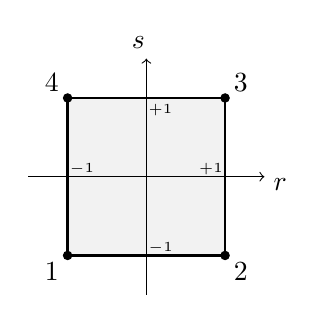
\begin{tikzpicture}
%\draw[step=0.5cm,gray,very thin] (0,0) grid (4,4); 
\draw[fill=gray!10,gray!10](1,1) rectangle (3,3);
\draw[thick] (1,1)--(3,1)--(3,3)--(1,3)--cycle;
\draw [->] (0.5,2) -- (3.5,2);
\draw [->] (2,0.5) -- (2,3.5);
\node[] at (3.7,1.9) {$r$};
\node[] at (1.9,3.7) {$s$};
\draw[black,fill=black] (1,1)   circle (1.5pt);
\draw[black,fill=black] (3,1)   circle (1.5pt);
\draw[black,fill=black] (3,3)   circle (1.5pt);
\draw[black,fill=black] (1,3)   circle (1.5pt);
\node[] at (0.8,0.8) {$1$};
\node[] at (0.8,3.2) {$4$};
\node[] at (3.2,0.8) {$2$};
\node[] at (3.2,3.2) {$3$};
\node[] at (1.18,2.1) {\tiny $-1$};
\node[] at (2.82,2.1) {\tiny $+1$};
\node[] at (2.18,1.1) {\tiny $-1$};
\node[] at (2.18,2.85) {\tiny $+1$};
\end{tikzpicture}
\end{center}



Note the counter-clockwise numbering\footnote{Note that in many of the python codes which 
are part of this project the numbering starts at 0.}.
This element is commonly called the reference element. How we go from the $(x,y)$ coordinate system 
to the $(r,s)$ once and vice versa will be dealt with later on.
The basis functions in the above reference element in the reduced 
coordinates system $(r,s)$ are given by:

\begin{mdframed}[backgroundcolor=blue!5]
\begin{eqnarray}
\bN_1(r,s)&=&0.25(1-r)(1-s) \nonumber\\
\bN_2(r,s)&=&0.25(1+r)(1-s) \nonumber\\
\bN_3(r,s)&=&0.25(1+r)(1+s) \nonumber\\
\bN_4(r,s)&=&0.25(1-r)(1+s) 
\end{eqnarray}
\end{mdframed}
These basis functions are the product of the linear basis functions of Section~\ref{sec:bf1}
in the $r$ direction and the $s$ direction.
The partial derivatives of these functions with respect to $r$ ans $s$ automatically follow:

\begin{mdframed}[backgroundcolor=blue!5]
\begin{align}
\frac{\partial \bN_1}{\partial r}(r,s)&= - 0.25(1-s) &
\frac{\partial \bN_1}{\partial s}(r,s)&= - 0.25(1-r) \nonumber\\
\frac{\partial \bN_2}{\partial r}(r,s)&= + 0.25(1-s) &
\frac{\partial \bN_2}{\partial s}(r,s)&= - 0.25(1+r) \nonumber\\
\frac{\partial \bN_3}{\partial r}(r,s)&= + 0.25(1+s) &
\frac{\partial \bN_3}{\partial s}(r,s)&= + 0.25(1+r) \nonumber\\
\frac{\partial \bN_4}{\partial r}(r,s)&= - 0.25(1+s) &
\frac{\partial \bN_4}{\partial s}(r,s)&= + 0.25(1-r) \nonumber
\end{align}
\end{mdframed}

Let us go back to Eq.~\eqref{bf01} and let us assume that the 
function $v(r,s)=C$ so that $v_i=C$ for $i=1,2,3,4$. 
It then follows that 
\[
v^h(r,s) = \sum_{i=1}^4 \bN_i(r,s)\;  v_i 
=C \sum_{i=1}^4 \bN_i(r,s)
=C [
\bN_1(r,s)
+\bN_2(r,s)
+\bN_3(r,s)
+\bN_4(r,s)]=C
\]
This is a very important property: if the $v$ function used to 
assign values at the vertices is constant, then 
the value of $v^h$ {\it anywhere} in the element is exactly $C$.
If we now turn to the derivatives of $v$ with respect to $r$ and $s$:
\[
\frac{\partial {v}^h}{\partial r}(r,s) 
= \sum_{i=1}^4 \frac{\partial \bN_i}{\partial r}(r,s)\;  v_i 
= C \sum_{i=1}^4 \frac{\partial \bN_i}{\partial r}(r,s) 
= C \left[ - 0.25(1-s)  + 0.25(1-s)  + 0.25(1+s)  - 0.25(1+s) \right] = 0 
\]

\[
\frac{\partial v^h}{\partial s}(r,s) 
= \sum_{i=1}^4 \frac{\partial \bN_i}{\partial s}(r,s)\;  v_i 
= C \sum_{i=1}^4 \frac{\partial \bN_i}{\partial s}(r,s) 
= C \left[ - 0.25(1-r) - 0.25(1+r) + 0.25(1+r) + 0.25(1-r) \right] = 0 
\]
We reassuringly find that the derivative of a constant field anywhere in the element is exactly zero.

If we now choose $v(r,s)=ar+bs$ with $a$ and $b$ two constant scalars, we find:
\begin{eqnarray}
v^h(r,s) 
&=& \sum_{i=1}^4 \bN_i(r,s)\;  v_i  \nn\\
&=& \sum_{i=1}^4 \bN_i(r,s) (ar_i+bs_i) \nn\\
&=& a \sum_{i=1}^4 \bN_i(r,s) r_i + b \sum_{i=1}^4 \bN_i(r,s) s_i \nn\\
&=& a \left[ 
 \frac14(1-r)(1-s)(-1)
+\frac14(1+r)(1-s)(+1)
+\frac14(1+r)(1+s)(+1)
+\frac14(1-r)(1+s)(-1) \right]  \nonumber\\
&+& b  
\left[ 
 \frac14(1-r)(1-s)(-1)
+\frac14(1+r)(1-s)(-1)
+\frac14(1+r)(1+s)(+1)
+\frac14(1-r)(1+s)(+1) \right]  \nonumber\\
&=& \frac{a}{4} \left[ 
-(1-r)(1-s)
+(1+r)(1-s)
+(1+r)(1+s)
-(1-r)(1+s) \right]  \nonumber\\
&+& \frac{b}{4}
\left[ 
-(1-r)(1-s)
-(1+r)(1-s)
+(1+r)(1+s)
+(1-r)(1+s) 
\right]  \nonumber\\
&=& ar+bs
\end{eqnarray}
This set of bilinear basis functions is therefore capable of exactly representing a bilinear field.
The derivatives are:
\begin{eqnarray}
\frac{\partial v^h}{\partial r}(r,s) 
&=& \sum_{i=1}^4 \frac{\partial \bN_i}{\partial r}(r,s)\;  v_i  \\
&=& a \sum_{i=1}^4 \frac{\partial \bN_i}{\partial r}(r,s) r_i 
+ b \sum_{i=1}^4 \frac{\partial \bN_i}{\partial r}(r,s) s_i \\
&=& a \left[
- \frac14(1-s)(-1) 
+ \frac14(1-s)(+1) 
+ \frac14(1+s)(+1) 
- \frac14(1+s)(-1) 
\right] \nonumber\\
&+&b \left[
- \frac14(1-s)(-1) 
+ \frac14(1-s)(-1) 
+ \frac14(1+s)(+1) 
- \frac14(1+s)(+1) 
\right] \nonumber\\
&=& \frac{a}{4} \left[
 (1-s)
+ (1-s)
+ (1+s)
+ (1+s)
\right] \nonumber\\
&+&\frac{b}{4} \left[
 (1-s)
- (1-s)
+ (1+s)
- (1+s)
\right] \nonumber\\
&=& a 
\end{eqnarray}
Here again, we find that the derivative of the bilinear field inside the element is exact: 
$\frac{\partial v^h}{\partial r} = \frac{\partial v}{\partial r}$.

However, following the same methodology as above, one can easily prove 
that this is no more true for polynomials of degree strictly higher than 1. 
This fact has serious consequences: if the solution to the problem at hand is 
for instance a parabola, the $Q_1$ basis functions cannot represent the solution properly, 
but only by approximating the parabola in each element by a line. As we will see 
later, $Q_2$ basis functions can remedy this problem by containing quadratic terms.

\begin{remark}
The $Q_1$ basis functions are first-order polynomials. We have seen that they can be used to compute
gradients. However they cannot be used to compute 2nd-order derivatives since their 2nd-order
derivative is identically zero.
\end{remark}




%%%%%%%%%%%%%%%%%%%%%%%%%%%%%%%%%%%%%%%%%%%%%%%%%%%%%%%%%%%%%%%%%%%%%%%%%%%%%%
\subsubsection{Biquadratic basis functions in 2D ($Q_2$)}\label{ss:q22d}
\index{general}{$Q_2$}

\begin{flushright} {\tiny {\color{gray} basis\_Q2\_2D.tex}} \end{flushright}
%~~~~~~~~~~~~~~~~~~~~~~~~~~~~~~~~~~~~~~~~~~~~~~~~~~~~~~~~~~~~~~~~~~~~~~~~~~~~~~~~~~~~~~~~~~~~~~~~~~

This element is part of the so-called Lagrange family \cite{raki00}. 
Inside an element the local numbering of the nodes is as follows\footnote{I have adopted here 
a numbering scheme starting at zero!}:

\begin{flushright} {\tiny {\color{gray} (tikz\_q22d.tex)}} \end{flushright}
%~~~~~~~~~~~~~~~~~~~~~~~~~~~~~~~~~~~~~~~~~~~~~~~~~~~~~~~~~~~~~~~~~~~~~~~~~~~~~~~~~~~~~~~~~~~~~~~~~~

\begin{center}
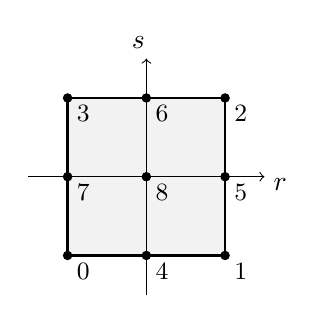
\begin{tikzpicture}
%\draw[step=0.5cm,gray,very thin] (0,0) grid (4,4); 
\draw[fill=gray!10,gray!10](1,1) rectangle (3,3);
\draw[thick] (1,1)--(3,1)--(3,3)--(1,3)--cycle;
\draw [->] (0.5,2) -- (3.5,2);
\draw [->] (2,0.5) -- (2,3.5);
\node[] at (3.7,1.9) {$r$};
\node[] at (1.9,3.7) {$s$};
\draw[black,fill=black] (1,1)   circle (1.5pt);
\draw[black,fill=black] (1,2)   circle (1.5pt);
\draw[black,fill=black] (1,3)   circle (1.5pt);
\draw[black,fill=black] (2,1)   circle (1.5pt);
\draw[black,fill=black] (2,2)   circle (1.5pt);
\draw[black,fill=black] (2,3)   circle (1.5pt);
\draw[black,fill=black] (3,1)   circle (1.5pt);
\draw[black,fill=black] (3,2)   circle (1.5pt);
\draw[black,fill=black] (3,3)   circle (1.5pt);
\node[] at (1.2,0.8) {\small $0$};
\node[] at (2.2,0.8) {\small $4$};
\node[] at (3.2,0.8) {\small $1$};
\node[] at (1.2,1.8) {\small $7$};
\node[] at (2.2,1.8) {\small $8$};
\node[] at (3.2,1.8) {\small $5$};
\node[] at (1.2,2.8) {\small $3$};
\node[] at (2.2,2.8) {\small $6$};
\node[] at (3.2,2.8) {\small $2$};
\end{tikzpicture}
\end{center}



Note that this numbering is also employed in Li \cite[p56]{li06}.
The polynomial representation of the function $\phi$ over this element is then
\[
\phi^h(r,s) = a + br + cs + drs + er^2 + fs^2 + gr^2s + hrs^2 + i r^2s^2 = \sum_{i=0}^8 \bN_i(r,s) \phi_i
\]
and one can show that the basis functions are:
\begin{mdframed}[backgroundcolor=blue!5]
\begin{eqnarray}
\bN_0(r,s)&=& \frac{1}{2}r(r-1)  \frac{1}{2}s(s-1)\nonumber\\
\bN_1(r,s)&=& \frac{1}{2}r(r+1)  \frac{1}{2}s(s-1)\nonumber\\
\bN_2(r,s)&=& \frac{1}{2}r(r+1)  \frac{1}{2}s(s+1)\nonumber\\
\bN_3(r,s)&=& \frac{1}{2}r(r-1)  \frac{1}{2}s(s+1)\nonumber\\
\bN_4(r,s)&=&     (1-r^2)  \frac{1}{2}s(s-1)\nonumber\\
\bN_5(r,s)&=& \frac{1}{2}r(r+1)      (1-s^2)\nonumber\\
\bN_6(r,s)&=&     (1-r^2)  \frac{1}{2}s(s+1)\nonumber\\
\bN_7(r,s)&=& \frac{1}{2}r(r-1)      (1-s^2)\nonumber\\
\bN_8(r,s)&=&     (1-r^2)      (1-s^2)\nonumber
\end{eqnarray}
\end{mdframed}

Note that we have $\bN_i(r_j,s_j)=\delta_{ij}$ and $\bN_i(r_i,s_i)=1$. 

Their derivatives are given by:
\begin{mdframed}[backgroundcolor=blue!5]
\begin{align}
\frac{\partial \bN_0}{\partial r}&= \frac{1}{2}(2r-1)  \frac{1}{2}s(s-1) & 
\frac{\partial \bN_0}{\partial s}&= \frac{1}{2}r(r-1)  \frac{1}{2}(2s-1)\nonumber\\
\frac{\partial \bN_1}{\partial r}&= \frac{1}{2}(2r+1)  \frac{1}{2}s(s-1) &
\frac{\partial \bN_1}{\partial s}&= \frac{1}{2}r(r+1)  \frac{1}{2}(2s-1)\nonumber\\
\frac{\partial \bN_2}{\partial r}&= \frac{1}{2}(2r+1)  \frac{1}{2}s(s+1) &
\frac{\partial \bN_2}{\partial s}&= \frac{1}{2}r(r+1)  \frac{1}{2}(2s+1)\nonumber\\
\frac{\partial \bN_3}{\partial r}&= \frac{1}{2}(2r-1)  \frac{1}{2}s(s+1) &
\frac{\partial \bN_3}{\partial s}&= \frac{1}{2}r(r-1)  \frac{1}{2}(2s+1)\nonumber\\
\frac{\partial \bN_4}{\partial r}&=       (-2r)  \frac{1}{2}s(s-1) &
\frac{\partial \bN_4}{\partial s}&=     (1-r^2)  \frac{1}{2}(2s-1)\nonumber\\
\frac{\partial \bN_5}{\partial r}&= \frac{1}{2}(2r+1)     (1-s^2)&
\frac{\partial \bN_5}{\partial s}&= \frac{1}{2}r(r+1)        (-2s)\nonumber\\
\frac{\partial \bN_6}{\partial r}&=       (-2r)  \frac{1}{2}s(s+1)&
\frac{\partial \bN_6}{\partial s}&=     (1-r^2)  \frac{1}{2}(2s+1)\nonumber\\
\frac{\partial \bN_7}{\partial r}&= \frac{1}{2}(2r-1)     (1-s^2)&
\frac{\partial \bN_7}{\partial s}&= \frac{1}{2}r(r-1)        (-2s)\nonumber\\
\frac{\partial \bN_8}{\partial r}&=       (-2r)     (1-s^2)&
\frac{\partial \bN_8}{\partial s}&=     (1-r^2)        (-2s)\nonumber
\end{align}
\end{mdframed}


%%%%%%%%%%%%%%%%%%%%%%%%%%%%%%%%%%%%%%%%%%%%%%%%%%%%%%%%%%%%%%%%%%%%%%%%%%%%%%
\subsubsection{Bicubic basis functions in 2D ($Q_3$)}
\index{general}{$Q_3$}

\begin{flushright} {\tiny {\color{gray} basis\_Q3\_2D.tex}} \end{flushright}
%~~~~~~~~~~~~~~~~~~~~~~~~~~~~~~~~~~~~~~~~~~~~~~~~~~~~~~~~~~~~~~~~~~~~~~~~~~~~~~~~~~~~~~~~~~~~~~~~~~

Inside an element the local numbering of the nodes is as follows:

\begin{flushright} {\tiny {\color{gray} (tikz\_q32d.tex)}} \end{flushright}
%~~~~~~~~~~~~~~~~~~~~~~~~~~~~~~~~~~~~~~~~~~~~~~~~~~~~~~~~~~~~~~~~~~~~~~~~~~~~~~~~~~~~~~~~~~~~~~~~~~


\begin{center}
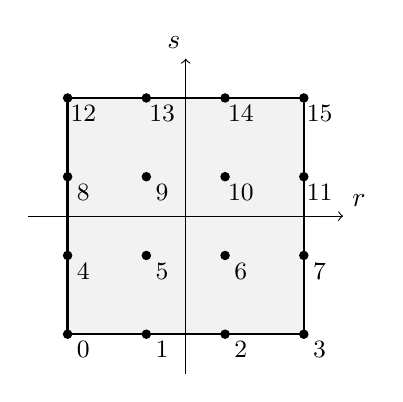
\begin{tikzpicture}
%\draw[step=0.5cm,gray,very thin] (0,0) grid (5,5); 
\draw[fill=gray!10,gray!10](1,1) rectangle (4,4);
\draw[thick] (1,1)--(4,1)--(4,4)--(1,4)--cycle;
\draw [->] (0.5,2.5) -- (4.5,2.5);
\draw [->] (2.5,0.5) -- (2.5,4.5);
\node[] at (4.7,2.7) {$r$};
\node[] at (2.35,4.7) {$s$};
\draw[black,fill=black] (1,1)   circle (1.5pt);
\draw[black,fill=black] (1,2)   circle (1.5pt);
\draw[black,fill=black] (1,3)   circle (1.5pt);
\draw[black,fill=black] (1,4)   circle (1.5pt);
\draw[black,fill=black] (2,1)   circle (1.5pt);
\draw[black,fill=black] (2,2)   circle (1.5pt);
\draw[black,fill=black] (2,3)   circle (1.5pt);
\draw[black,fill=black] (2,4)   circle (1.5pt);
\draw[black,fill=black] (3,1)   circle (1.5pt);
\draw[black,fill=black] (3,2)   circle (1.5pt);
\draw[black,fill=black] (3,3)   circle (1.5pt);
\draw[black,fill=black] (3,4)   circle (1.5pt);
\draw[black,fill=black] (4,1)   circle (1.5pt);
\draw[black,fill=black] (4,2)   circle (1.5pt);
\draw[black,fill=black] (4,3)   circle (1.5pt);
\draw[black,fill=black] (4,4)   circle (1.5pt);
\node[] at (1.2,0.8) {\small $0$};
\node[] at (2.2,0.8) {\small $1$};
\node[] at (3.2,0.8) {\small $2$};
\node[] at (4.2,0.8) {\small $3$};
\node[] at (1.2,1.8) {\small $4$};
\node[] at (2.2,1.8) {\small $5$};
\node[] at (3.2,1.8) {\small $6$};
\node[] at (4.2,1.8) {\small $7$};
\node[] at (1.2,2.8) {\small $8$};
\node[] at (2.2,2.8) {\small $9$};
\node[] at (3.2,2.8) {\small $10$};
\node[] at (4.2,2.8) {\small $11$};
\node[] at (1.2,3.8) {\small $12$};
\node[] at (2.2,3.8) {\small $13$};
\node[] at (3.2,3.8) {\small $14$};
\node[] at (4.2,3.8) {\small $15$};
\end{tikzpicture}
\end{center}



The 1D cubic basis functions are given by:
\begin{align}
\bN_1(r)&=(-1   +r +9r^2 - 9r^3)/16 & \bN_1(t)&=(-1   +t +9t^2 - 9t^3)/16 \nonumber\\
\bN_2(r)&=(+9 -27r -9r^2 +27r^3)/16 & \bN_2(t)&=(+9 -27t -9t^2 +27t^3)/16 \nonumber\\
\bN_3(r)&=(+9 +27r -9r^2 -27r^3)/16 & \bN_3(t)&=(+9 +27t -9t^2 -27t^3)/16 \nonumber\\
\bN_4(r)&=(-1   -r +9r^2 + 9r^3)/16 & \bN_4(t)&=(-1   -t +9t^2 + 9t^3)/16 \nonumber
\end{align}

The resulting basis functions are simply the tensor product of the above 1D ones:

\begin{mdframed}[backgroundcolor=blue!5]
\begin{eqnarray}
\bN_{01}(r,s)&=&\bN_1(r)\bN_1(s) = (-1   +r +9r^2 - 9r^3)/16 \cdot (-1  +t +9s^2 - 9s^3)/16 \nonumber\\
\bN_{02}(r,s)&=&\bN_2(r)\bN_1(s) = (+9 -27r -9r^2 +27r^3)/16 \cdot (-1  +t +9s^2 - 9s^3)/16 \nonumber\\
\bN_{03}(r,s)&=&\bN_3(r)\bN_1(s) = (+9 +27r -9r^2 -27r^3)/16 \cdot (-1  +t +9s^2 - 9s^3)/16 \nonumber\\
\bN_{04}(r,s)&=&\bN_4(r)\bN_1(s) = (-1   -r +9r^2 + 9r^3)/16 \cdot (-1  +t +9s^2 - 9s^3)/16 \nonumber\\
\bN_{05}(r,s)&=&\bN_1(r)\bN_2(s) = (-1   +r +9r^2 - 9r^3)/16 \cdot (9 -27s -9s^2 +27s^3)/16 \nonumber\\
\bN_{06}(r,s)&=&\bN_2(r)\bN_2(s) = (+9 -27r -9r^2 +27r^3)/16 \cdot (9 -27s -9s^2 +27s^3)/16 \nonumber\\
\bN_{07}(r,s)&=&\bN_3(r)\bN_2(s) = (+9 +27r -9r^2 -27r^3)/16 \cdot (9 -27s -9s^2 +27s^3)/16 \nonumber\\
\bN_{08}(r,s)&=&\bN_4(r)\bN_2(s) = (-1   -r +9r^2 + 9r^3)/16 \cdot (9 -27s -9s^2 +27s^3)/16 \nonumber\\
\bN_{09}(r,s)&=&\bN_1(r)\bN_3(s) = (-1   +r +9r^2 - 9r^3)/16 \cdot (9 +27t -9t^2 -27t^3)/16 \nn\\
\bN_{10}(r,s)&=&\bN_2(r)\bN_3(s) = (+9 -27r -9r^2 +27r^3)/16 \cdot (9 +27t -9t^2 -27t^3)/16 \nn\\
\bN_{11}(r,s)&=&\bN_3(r)\bN_3(s) = (+9 +27r -9r^2 -27r^3)/16 \cdot (9 +27t -9t^2 -27t^3)/16 \nn\\
\bN_{12}(r,s)&=&\bN_4(r)\bN_3(s) = (-1   -r +9r^2 + 9r^3)/16 \cdot (9 +27t -9t^2 -27t^3)/16 \nn\\
\bN_{13}(r,s)&=&\bN_1(r)\bN_4(s) = (-1   +r +9r^2 - 9r^3)/16 \cdot (-1   -t +9t^2 + 9t^3)/16\nn\\
\bN_{14}(r,s)&=&\bN_2(r)\bN_4(s) = (+9 -27r -9r^2 +27r^3)/16 \cdot (-1   -t +9t^2 + 9t^3)/16\nn\\
\bN_{15}(r,s)&=&\bN_3(r)\bN_4(s) = (+9 +27r -9r^2 -27r^3)/16 \cdot (-1   -t +9t^2 + 9t^3)/16\nn\\
\bN_{16}(r,s)&=&\bN_4(r)\bN_4(s) = (-1   -r +9r^2 + 9r^3)/16 \cdot (-1   -t +9t^2 + 9t^3)/16
\end{eqnarray}
\end{mdframed}

\begin{center}
\includegraphics[width=4cm]{images/basis_Q3_2D/N1}
\includegraphics[width=4cm]{images/basis_Q3_2D/N2}
\includegraphics[width=4cm]{images/basis_Q3_2D/N3}
\includegraphics[width=4cm]{images/basis_Q3_2D/N4}\\
\includegraphics[width=4cm]{images/basis_Q3_2D/N5}
\includegraphics[width=4cm]{images/basis_Q3_2D/N6}
\includegraphics[width=4cm]{images/basis_Q3_2D/N7}
\includegraphics[width=4cm]{images/basis_Q3_2D/N8}\\
\includegraphics[width=4cm]{images/basis_Q3_2D/N9}
\includegraphics[width=4cm]{images/basis_Q3_2D/N10}
\includegraphics[width=4cm]{images/basis_Q3_2D/N11}
\includegraphics[width=4cm]{images/basis_Q3_2D/N12}\\
\includegraphics[width=4cm]{images/basis_Q3_2D/N13}
\includegraphics[width=4cm]{images/basis_Q3_2D/N14}
\includegraphics[width=4cm]{images/basis_Q3_2D/N15}
\includegraphics[width=4cm]{images/basis_Q3_2D/N16}\\
{\captionfont Surface representation of the basis functions on the reference element.\\
{\color{gray} in images/basis\_Q3\_2D/ }}
\end{center}

The derivatives are trivial to obtain from the derivatives of the 1D basis functions, 
e.g.
\[
\frac{\partial \bN_{13}}{\partial r} = 
\frac{\partial \bN_{1}}{\partial r} \bN_4(s) 
\]

These basis functions are used in \stone 19.










%%%%%%%%%%%%%%%%%%%%%%%%%%%%%%%%%%%%%%%%%%%%%%%%%%%%%%%%%%%%%%%%%%%%%
\subsubsection{Eight node serendipity basis functions in 2D ($Q_2^{(8)}$)}
\label{sec:serendipity2D}
\index{general}{$Q_2^{(8)}$} 
\index{general}{Serendipity element}

\begin{flushright} {\tiny {\color{gray} basis\_Q28\_2D.tex}} \end{flushright}
%~~~~~~~~~~~~~~~~~~~~~~~~~~~~~~~~~~~~~~~~~~~~~~~~~~~~~~~~~~~~~~~~~~~~~~~~~~~~~~~~~~~~~~~~~~~~~~~~~~

The serendipity elements are those rectangular elements which have no
interior nodes (See for example Reddy \cite[p65]{reddybook2}).
Inside an element a possible local numbering of the nodes is as follows:

\input{tikz/tikz_serendipity2D}

The main difference with the $Q_2$ element resides in the fact that there is 
no node in the middle of the element.
The polynomial representation of the function $\phi$ over the element is then
\[
\phi_h(r,s) = a + br + cs + drs + er^2 + fs^2 + gr^2s + hrs^2
\]
Note that absence of the $r^2s^2$ term which was previously associated 
to the center node. We find that 
\begin{mdframed}[backgroundcolor=blue!5]
\begin{eqnarray}
\bN_0(r,s)&=& \frac{1}{4}(1-r)(1-s)(-r-s-1) \\
\bN_1(r,s)&=& \frac{1}{4}(1+r)(1-s)(r-s-1) \\
\bN_2(r,s)&=& \frac{1}{4}(1+r)(1+s)(r+s-1) \\
\bN_3(r,s)&=& \frac{1}{4}(1-r)(1+s)(-r+s-1) \\
\bN_4(r,s)&=& \frac{1}{2}(1-r^2)(1-s)  \\
\bN_5(r,s)&=& \frac{1}{2}(1+r)  (1-s^2)\\
\bN_6(r,s)&=& \frac{1}{2}(1-r^2)(1+s)  \\
\bN_7(r,s)&=& \frac{1}{2}(1-r)  (1-s^2)
\end{eqnarray}
\end{mdframed}

The basis functions at the mid side nodes are products of a 
second order polynomial parallel to side and 
a linear function perpendicular to the side
while basis functions for corner nodes are modifications of the bilinear
quadrilateral element.

\begin{center}
\includegraphics[width=4cm]{images/basis_Q28_2D/N1}
\includegraphics[width=4cm]{images/basis_Q28_2D/N2}
\includegraphics[width=4cm]{images/basis_Q28_2D/N3}
\includegraphics[width=4cm]{images/basis_Q28_2D/N4}\\
\includegraphics[width=4cm]{images/basis_Q28_2D/N5}
\includegraphics[width=4cm]{images/basis_Q28_2D/N6}
\includegraphics[width=4cm]{images/basis_Q28_2D/N7}
\includegraphics[width=4cm]{images/basis_Q28_2D/N8}\\
{\captionfont Surface representation of the basis functions on the reference element.
{\color{gray} in images/basis\_Q28\_2D/ }}
\end{center}



The first-order derivatives are given by:

\begin{mdframed}[backgroundcolor=blue!5]
\begin{eqnarray}
\frac{\partial \bN_0}{\partial r}(r,s)&=& -\frac{1}{4}(s-1)(2r+s)  \\
\frac{\partial \bN_1}{\partial r}(r,s)&=& -\frac{1}{4}(s-1)(2r-s)  \\
\frac{\partial \bN_2}{\partial r}(r,s)&=& \frac{1}{4}(s+1)(2r+s)  \\
\frac{\partial \bN_3}{\partial r}(r,s)&=& \frac{1}{4}(s+1)(2r-s)  \\
\frac{\partial \bN_4}{\partial r}(r,s)&=& r(s-1)  \\
\frac{\partial \bN_5}{\partial r}(r,s)&=& \frac{1}{2} (1-s^2)  \\
\frac{\partial \bN_6}{\partial r}(r,s)&=& -r(s+1)  \\
\frac{\partial \bN_7}{\partial r}(r,s)&=& -\frac{1}{2} (1-s^2)  
\end{eqnarray}
\end{mdframed}

\begin{mdframed}[backgroundcolor=blue!5]
\begin{eqnarray}
\frac{\partial \bN_0}{\partial s}(r,s)&=& -\frac{1}{4}(r-1)(r+2s) \\
\frac{\partial \bN_1}{\partial s}(r,s)&=& -\frac{1}{4}(r+1)(r-2s) \\
\frac{\partial \bN_2}{\partial s}(r,s)&=&  \frac{1}{4}(r+1)(r+2s) \\
\frac{\partial \bN_3}{\partial s}(r,s)&=&  \frac{1}{4}(r-1)(r-2s) \\
\frac{\partial \bN_4}{\partial s}(r,s)&=& - \frac{1}{2}(1-r^2)\\
\frac{\partial \bN_5}{\partial s}(r,s)&=&  -(r+1)s \\
\frac{\partial \bN_6}{\partial s}(r,s)&=& \frac{1}{2} (1-r^2)\\
\frac{\partial \bN_7}{\partial s}(r,s)&=&  (r-1)s
\end{eqnarray}
\end{mdframed}
These basis functions are used in \stone 52.













%%%%%%%%%%%%%%%%%%%%%%%%%%%%%%%%%%%%%%%%%%%%%%%%%%%%%%%%%%%%%%%%%%%%%
\subsubsection{Eight node serendipity basis functions in 2D ($QH8-C1$)}
\label{sec:serendipity2Db}
\index{general}{$QH8-C1$} \index{general}{Serendipity element}

This element is proposed in Zhang \& Xiang (2020) \cite{zhxi20}. Two remarks
must be made: 1) Eq.~(29) of their publication which is the definition
of the basis functions contains an error\footnote{
Answer from the author: "N5 to N8 is missing an A in the denominator and 
the calculation program does not have this problem"}. 2) The authors use a rather 
uncommon and annoying rotated numbering:
\begin{verbatim}
      y
      |
2=====5=====1             3=====6=====2
|           |             |           |   (r_0,s_0)=(-1,-1)   (r_4,s_4)=( 0,-1)
|           |             |           |   (r_1,s_1)=(+1,-1)   (r_5,s_5)=(+1, 0)
6           8--x          7     +     5   (r_2,s_2)=(+1,+1)   (r_6,s_6)=( 0,+1)
|           |             |           |   (r_3,s_3)=(-1,+1)   (r_7,s_7)=(-1, 0)
|           |             |           |    
3=====7=====4             0=====4=====1
Zhang & Xiang             our numbering
\end{verbatim}

For each element they define (their numbering):
\begin{eqnarray}
A   &=& \frac{1}{2} [ (x_1-x_3)(y_2-y_4)-(x_2-x_4)(y_1-y_3) ] \nn\\
m_x &=& (x_1-x_4)(y_2-y_3)-(x_2-x_3)(y_1-y_4) \nn\\
m_y &=& (x_3-x_4)(y_1-y_2)-(x_1-x_2)(y_3-y_4) \nn
\end{eqnarray}

Note that $A$ is the area of the element, and that in the case when 
the element is a rectangle then $m_x=m_y=0$.

\begin{eqnarray}
\bN_1(r,s)&=& n_1(r,s) +(m_x^2 - m_xm_y + m_y^2)\frac{E(r,s)}{D} \nn\\
\bN_2(r,s)&=& n_2(r,s) +(m_x^2 + m_xm_y + m_y^2)\frac{E(r,s)}{D} \nn\\
\bN_3(r,s)&=& n_3(r,s) +(m_x^2 - m_xm_y + m_y^2)\frac{E(r,s)}{D} \nn\\
\bN_4(r,s)&=& n_4(r,s) +(m_x^2 + m_xm_y + m_y^2)\frac{E(r,s)}{D} \nn\\
\bN_5(r,s)&=& n_5(r,s) -m_x(2Am_x+m_y^2)\frac{E(r,s)}{AD} \nn\\
\bN_6(r,s)&=& n_6(r,s) -m_y(2Am_y+m_x^2)\frac{E(r,s)}{AD} \nn\\
\bN_7(r,s)&=& n_7(r,s) +m_x(-2Am_x+m_y^2)\frac{E(r,s)}{AD} \nn\\
\bN_8(r,s)&=& n_8(r,s) +m_y(-2Am_y+m_x^2)\frac{E(r,s)}{AD} \nn
\end{eqnarray}
with 
\[
E(r,s)=(1-r^2)(1-s^2)
\qquad
D=4(4A^2+m_x^2+m_y^2)
\]
and where the $n_i$ functions are the basis functions of the 'regular' 
8-node element (see Section~\ref{sec:serendipity2D}).

This is implemented in \stone 52.

\todo[inline]{not finished. SHOW CONSISTENCY !! like in paper
email sent to author about mistake.  }








%%%%%%%%%%%%%%%%%%%%%%%%%%%%%%%%%%%%
\subsubsection{Biquartic basis functions in 2D ($Q_4$)}
\index{general}{$Q_4$}

Inside an element the local numbering of the nodes is as follows:

\begin{flushright} {\tiny {\color{gray} (tikz\_q42d.tex)}} \end{flushright}
%~~~~~~~~~~~~~~~~~~~~~~~~~~~~~~~~~~~~~~~~~~~~~~~~~~~~~~~~~~~~~~~~~~~~~~~~~~~~~~~~~~~~~~~~~~~~~~~~~~


\begin{center}
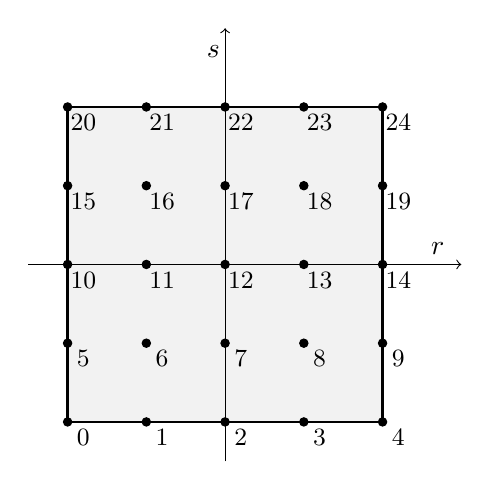
\begin{tikzpicture}
%\draw[step=0.5cm,gray,very thin] (0,0) grid (5,5); 
\draw[fill=gray!10,gray!10](1,1) rectangle (5,5);
\draw[thick] (1,1)--(5,1)--(5,5)--(1,5)--cycle;
\draw [->] (0.5,3) -- (6,3);
\draw [->] (3,0.5) -- (3,6);
\node[] at (5.7,3.2) {$r$};
\node[] at (2.85,5.7) {$s$};
\draw[black,fill=black] (1,1)   circle (1.5pt);
\draw[black,fill=black] (1,2)   circle (1.5pt);
\draw[black,fill=black] (1,3)   circle (1.5pt);
\draw[black,fill=black] (1,4)   circle (1.5pt);
\draw[black,fill=black] (1,5)   circle (1.5pt);

\draw[black,fill=black] (2,1)   circle (1.5pt);
\draw[black,fill=black] (2,2)   circle (1.5pt);
\draw[black,fill=black] (2,3)   circle (1.5pt);
\draw[black,fill=black] (2,4)   circle (1.5pt);
\draw[black,fill=black] (2,5)   circle (1.5pt);

\draw[black,fill=black] (3,1)   circle (1.5pt);
\draw[black,fill=black] (3,2)   circle (1.5pt);
\draw[black,fill=black] (3,3)   circle (1.5pt);
\draw[black,fill=black] (3,4)   circle (1.5pt);
\draw[black,fill=black] (3,5)   circle (1.5pt);

\draw[black,fill=black] (4,1)   circle (1.5pt);
\draw[black,fill=black] (4,2)   circle (1.5pt);
\draw[black,fill=black] (4,3)   circle (1.5pt);
\draw[black,fill=black] (4,4)   circle (1.5pt);
\draw[black,fill=black] (4,5)   circle (1.5pt);

\draw[black,fill=black] (5,1)   circle (1.5pt);
\draw[black,fill=black] (5,2)   circle (1.5pt);
\draw[black,fill=black] (5,3)   circle (1.5pt);
\draw[black,fill=black] (5,4)   circle (1.5pt);
\draw[black,fill=black] (5,5)   circle (1.5pt);

\node[] at (1.2,0.8) {\small $0$};
\node[] at (2.2,0.8) {\small $1$};
\node[] at (3.2,0.8) {\small $2$};
\node[] at (4.2,0.8) {\small $3$};
\node[] at (5.2,0.8) {\small $4$};

\node[] at (1.2,1.8) {\small $5$};
\node[] at (2.2,1.8) {\small $6$};
\node[] at (3.2,1.8) {\small $7$};
\node[] at (4.2,1.8) {\small $8$};
\node[] at (5.2,1.8) {\small $9$};

\node[] at (1.2,2.8) {\small $10$};
\node[] at (2.2,2.8) {\small $11$};
\node[] at (3.2,2.8) {\small $12$};
\node[] at (4.2,2.8) {\small $13$};
\node[] at (5.2,2.8) {\small $14$};

\node[] at (1.2,3.8) {\small $15$};
\node[] at (2.2,3.8) {\small $16$};
\node[] at (3.2,3.8) {\small $17$};
\node[] at (4.2,3.8) {\small $18$};
\node[] at (5.2,3.8) {\small $19$};

\node[] at (1.2,4.8) {\small $20$};
\node[] at (2.2,4.8) {\small $21$};
\node[] at (3.2,4.8) {\small $22$};
\node[] at (4.2,4.8) {\small $23$};
\node[] at (5.2,4.8) {\small $24$};

\end{tikzpicture}
\end{center}



%.....................................................................
\subsubsection{Linear basis functions for triangles in 2D ($P_1$)}\label{ss:p1}
\index{general}{$P_1$}

\begin{flushright} {\tiny {\color{gray} basis\_P1\_2D.tex}} \end{flushright}
%~~~~~~~~~~~~~~~~~~~~~~~~~~~~~~~~~~~~~~~~~~~~~~~~~~~~~~~~~~~~~~~~~~~~~~~~~~~~~~~~~~~~~~~~~~~~~~~~~~

Here we do not start from a reference element but consider instead a generic triangle:

\begin{flushright} {\tiny {\color{gray} (tikz\_P1.tex)}} \end{flushright}
%~~~~~~~~~~~~~~~~~~~~~~~~~~~~~~~~~~~~~~~~~~~~~~~~~~~~~~~~~~~~~~~~~~~~~~~~~~~~~~~~~~~~~~~~~~~~~~~~~~

\begin{center}
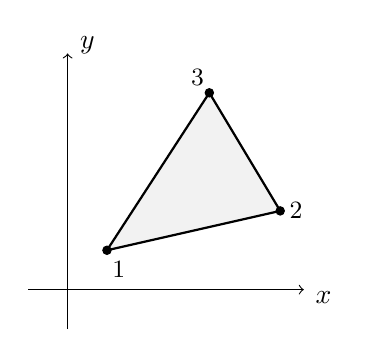
\begin{tikzpicture}
%\draw[step=0.5cm,gray,very thin] (0,0) grid (4,4); 
\draw[fill=gray!10,gray!10](1,1) (1,1)--(3.2,1.5)--(2.3,3)--cycle;
\draw[thick] (1,1)--(3.2,1.5)--(2.3,3)--cycle;
\draw [->] (0,0.5) -- (3.5,0.5);
\draw [->] (0.5,0) -- (0.5,3.5);
\node[] at (3.75,0.4) {$x$};
\node[] at (0.75,3.6) {$y$};
\draw[black,fill=black] (1,1)   circle (1.5pt);
\draw[black,fill=black] (3.2,1.5)   circle (1.5pt);
\draw[black,fill=black] (2.3,3)   circle (1.5pt);
\node[] at (1.15,0.75) {\small $1$};
\node[] at (3.4,1.5) {\small $2$};
\node[] at (2.15,3.2) {\small $3$};
\end{tikzpicture}
\end{center}




This is the simplest 2D element, which is also called linear triangular element.
Velocities (or displacements) $(u^h,v^h)$ in the element are interpolated from nodal velocities
$(u_i,v_i)$ using basis functions $\bN_i$ as follows,
\begin{small}
\[
\vec\upnu^h=
\left(
\begin{array}{c}
u^h(x,y) \\v^h(x,y)
\end{array}
\right)
=
\left(
\begin{array}{c}
\sum\limits_{i=1}^3 \bN_i(x,y) u_i \\
\sum\limits_{i=1}^3 \bN_i(x,y) v_i
\end{array}
\right)
=
\left(
\begin{array}{cccccc}
\bN_1(x,y) & 0 & \bN_2(x,y) & 0 & \bN_3(x,y) & 0\\
0 & \bN_1(x,y) & 0 & \bN_2(x,y) & 0 & \bN_3(x,y)\\
\end{array}
\right)
\cdot
\left(
\begin{array}{c}
u_1 \\ v_1 \\ u_2 \\ v_2 \\ u_3 \\ v_3
\end{array}
\right)
\]
\end{small}

For this element, we have three nodes at the vertices of the triangle, which are 
numbered around the element in the counterclockwise direction. 
Each node has two degrees of freedom (i.e. it can move in the $x$ and $y$ directions). 
The velocities $u^h$ and $v^h$ are assumed to be linear functions within the element, that is, 
\begin{eqnarray}
u^h(x,y)&=&b_1 +b_2x+b_3y \nn\\
v^h(x,y)&=&b_4 +b_5x+b_6y
\end{eqnarray}
where $b_i$ are constants to be determined and which depend on the triangle shape.
Note that the strain rate components are then given by
\begin{eqnarray}
\dot\varepsilon_{xx}(\vec\upnu)&=&b_2  \nn\\
\dot\varepsilon_{yy}(\vec\upnu)&=&b_6  \nn\\
\dot\varepsilon_{xy}(\vec\upnu)&=&(b_3+b_5)/2 \nn
\end{eqnarray}
and are constant throughout the element.

The velocities should satisfy the following six equations (when it is evaluated at a node we should 
recover the nodal velocity):
\begin{eqnarray}
u_1 &=& u^h(x_1,y_1)= b_1 + b_2x_1+b_3y_1 \nn\\
u_2 &=& u^h(x_2,y_2)= b_1 + b_2x_2+b_3y_2 \nn\\
u_3 &=& u^h(x_3,y_3)= b_1 + b_2x_3+b_3y_3 \nn\\
v_1 &=& v^h(x_1,y_1)= b_4 + b_5x_1+b_6y_1 \nn\\
v_2 &=& v^h(x_2,y_2)= b_4 + b_5x_2+b_6y_2 \nn\\
v_3 &=& v^h(x_3,y_3)= b_4 + b_5x_3+b_6y_3 \nn
\end{eqnarray}
Let us focus on the three equations with the $u$ component of the velocity.
These can be re-written:
\[
\left(
\begin{array}{c}
u_1 \\ u_2 \\ u_3  
\end{array}
\right)
=
\left(
\begin{array}{ccc}
1 & x_1 & y_1 \\
1 & x_2 & y_2 \\
1 & x_3 & y_3 \\
\end{array}
\right)
\cdot
\left(
\begin{array}{c}
b_1 \\ b_2 \\ b_3  
\end{array}
\right)
\]
In order to obtain $b_1,b_2,b_3$ we need to solve this system, or simply to compute the
inverse of the $3\times 3$ ${\bm M}$ matrix, as explained in Appendix~\ref{sec:inv3x3}.
We define $D={\rm det}({\bm M})$ and we get
\[
\left(
\begin{array}{c}
b_1 \\ b_2 \\ b_3  
\end{array}
\right)
=
\frac{1}{D}
\tilde{\bm M}
\cdot
\left(
\begin{array}{c}
u_1 \\ u_2 \\ u_3  
\end{array}
\right)
%\qquad
%{\rm and}
%\qquad
%\left(
%\begin{array}{c}
%b_4 \\ b_5 \\ b_6  
%\end{array}
%\right)
%=
%\frac{1}{D}
%\tilde{\bm M}
%\cdot
%\left(
%\begin{array}{c}
%v_1 \\ v_2 \\ v_3  
%\end{array}
%\right)
\]
The matrix $\tilde{\bm M}$ is given by:
\[
\tilde{\bm M}
%=
%\left(
%\begin{array}{ccc}
%  x_2y_3-x_3y_2  & -(y_3-y_2) &   x_3-x_2 \\
%-(x_1y_3-x_3y_1) &   y_3-y_1  & -(x_3-x_1) \\
%  x_1y_2-x_2y_1  & -(y_2-y_1) &   x_2-x_1
%\end{array}
%\right)
=
\left(
\begin{array}{ccc}
x_2y_3-x_3y_2 & x_3y_1-x_1y_3 & x_1y_2-x_2y_1 \\
y_2-y_3 & y_3-y_1  & y_1-y_2 \\
x_3-x_2 & x_1-x_3 & x_2-x_1 
\end{array}
\right)
\]
so that 
\begin{eqnarray}
b_1 &=& \frac1D [ (x_2y_3-x_3y_2)u_1 + (x_3y_1-x_1y_3)u_2 + (x_1y_2-x_2y_1)u_3 ] \nn\\
b_2 &=& \frac1D [ (y_2-y_3)u_1 + (y_3-y_1)u_2 + (y_1-y_2)u_3 ] \nn\\
b_3 &=& \frac1D [ (x_3-x_2)u_1 + (x_1-x_3)u_2 + (x_2-x_1)u_3 ]
\end{eqnarray}
We then have
\begin{eqnarray}
u^h(x,y) 
&=& b_1 + b_2 x + b_3 y \nn\\
&=&\frac1D [(x_2y_3-x_3y_2)u_1 + (x_3y_1-x_1y_3)u_2 + (x_1y_2-x_2y_1)u_3 ] \nn\\
&+&\frac1D [(y_2-y_3)u_1 + (y_3-y_1)u_2 + (y_1-y_2)u_3]x \nn\\
&+&\frac1D [(x_3-x_2)u_1 + (x_1-x_3)u_2 + (x_2-x_1)u_3]y \nn\\
&=&\frac1D [(x_2y_3-x_3y_2) + (y_2-y_3)x + (x_3-x_2)y]u_1\nn\\ 
&+&\frac1D [(x_3y_1-x_1y_3) + (y_3-y_1) x + (x_1-x_3) y]u_2 \nn\\
&+&\frac1D [(x_1y_2-x_2y_1) + (y_1-y_2) x + (x_2-x_1) y]u_3\nn\\
&=& \bN_1(x,y) u_1 + \bN_2(x,y) u_2 + \bN_3(x,y) u_3
\end{eqnarray}
with the linear basis functions are given by:
\begin{eqnarray}
\bN_1(x,y) &=& \frac{1}{D}[(x_2y_3-x_3y_2) + (y_2-y_3)x + (x_3-x_2)y] \nn\\
\bN_2(x,y) &=& \frac{1}{D}[(x_3y_1-x_1y_3) + (y_3-y_1)x + (x_1-x_3)y] \nn\\
\bN_3(x,y) &=& \frac{1}{D}[(x_1y_2-x_2y_1) + (y_1-y_2)x + (x_2-x_1)y] \nn
\end{eqnarray}
We can then easily verify that for example
\begin{eqnarray}
\bN_2(x_1,y_1)&=& \frac{1}{D}[(x_3y_1-x_1y_3) + (y_3-y_1)x_1 + (x_1-x_3)y_1] = 0 \\
\bN_2(x_2,y_2)&=& \frac{1}{D}[(x_3y_1-x_1y_3) + (y_3-y_1)x_2 + (x_1-x_3)y_2] = 1 \\
\bN_2(x_3,y_3)&=& \frac{1}{D}[(x_3y_1-x_1y_3) + (y_3-y_1)x_3 + (x_1-x_3)y_3] = 0 
\end{eqnarray}
Note that the area $A$ of the triangle is given by:
\[
A=\frac{1}{2}D = \frac{1}{2}
\left|
\begin{array}{ccc}
1 & x_1 & y_1 \\
1 & x_2 & y_2 \\
1 & x_3 & y_3 
\end{array}
\right|
\]

\noindent If we now consider the reference element in the reduced coordinates space $(r,s)$:

\begin{flushright} {\tiny {\color{gray} (tikz\_P1ref.tex)}} \end{flushright}
%~~~~~~~~~~~~~~~~~~~~~~~~~~~~~~~~~~~~~~~~~~~~~~~~~~~~~~~~~~~~~~~~~~~~~~~~~~~~~~~~~~~~~~~~~~~~~~~~~~


\begin{center}
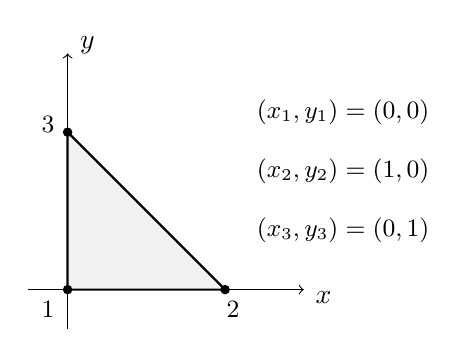
\begin{tikzpicture}
%\draw[step=0.5cm,gray,very thin] (0,0) grid (4,4); 
\draw[fill=gray!10,gray!10] (0.5,0.5)--(2.5,0.5)--(0.5,2.5)--cycle;
\draw[thick] (0.5,0.5)--(2.5,0.5)--(0.5,2.5)--cycle;
\draw [->] (0,0.5) -- (3.5,0.5);
\draw [->] (0.5,0) -- (0.5,3.5);
\node[] at (3.75,0.4) {$x$};
\node[] at (0.75,3.6) {$y$};
\draw[black,fill=black] (0.5,0.5)   circle (1.5pt);
\draw[black,fill=black] (2.5,0.5)   circle (1.5pt);
\draw[black,fill=black] (0.5,2.5)   circle (1.5pt);
\node[] at (0.25,0.25) {\small $1$};
\node[] at (2.6,0.25) {\small $2$};
\node[] at (0.25,2.6) {\small $3$};
\node[] at (4,2.75) {\small $(x_1,y_1)=(0,0)$};
\node[] at (4,2) {\small $(x_2,y_2)=(1,0)$};
\node[] at (4,1.25) {\small $(x_3,y_3)=(0,1)$};
\end{tikzpicture}
\end{center}



The basis polynomial is then
\[
f(r,s) = a + br + cs 
\]
and the basis functions:
\begin{mdframed}[backgroundcolor=blue!5]
\begin{eqnarray}
\bN_0(r,s) &=& 1-r-s \\
\bN_1(r,s) &=& r \\
\bN_2(r,s) &=& s 
\end{eqnarray}
\end{mdframed}
Once again we can verify that $\bN_i(x_j,y_j)=\delta_{ij}$ and $\sum\limits_i \bN_i(r,s)=1$.


Coming back to the basis functions given for a generic triangle, we have
\begin{eqnarray}
\bN_1(x,y) &=& \frac{1}{D}[(x_2y_3-x_3y_2) + (y_2-y_3)x + (x_3-x_2)y] \nn\\
\bN_2(x,y) &=& \frac{1}{D}[(x_3y_1-x_1y_3) + (y_3-y_1)x + (x_1-x_3)y] \nn\\
\bN_3(x,y) &=& \frac{1}{D}[(x_1y_2-x_2y_1) + (y_1-y_2)x + (x_2-x_1)y] \nn
\end{eqnarray}
or, introducing the notations $x_{ij}=x_i-x_j$ and $y_{ij}=y_i-y_j$:
\begin{eqnarray}
\bN_1(x,y) &=& \frac{1}{D}[(x_2y_3-x_3y_2) + y_{23} x + x_{32} y] \nn\\
\bN_2(x,y) &=& \frac{1}{D}[(x_3y_1-x_1y_3) + y_{31} x + x_{13} y] \nn\\
\bN_3(x,y) &=& \frac{1}{D}[(x_1y_2-x_2y_1) + y_{12} x + x_{21} y] \nn
\end{eqnarray}
with $D=2|T|$ with $|T|$ being the area of the triangle.



The gradient matrix is then given by (see for example \cite{koko07}) 
\[
{\bm B} = 
\frac{1}{2|T|}
\begin{pmatrix}
\partial_x \bN_1 & 0 & \partial_x \bN_2 & 0 & \partial_x \bN_3 & 0 \\
0 & \partial_y \bN_1 & 0 & \partial_y \bN_2 & 0 & \partial_y \bN_3 \\
\partial_y \bN_1 & \partial_x \bN_1 &
\partial_y \bN_2 & \partial_x \bN_2 &
\partial_y \bN_3 & \partial_x \bN_3 
\end{pmatrix}
= \frac{1}{2|T|} \tilde{\bm B}
\]
with 
\[
\tilde{\bm B}=
\begin{pmatrix}
y_{23} & 0 & y_{31} & 0 & y_{12} & 0 \\
0 & x_{32} & 0 & x_{13} & 0 & x_{21} \\
x_{32} & y_{23} & x_{13} & y_{31} & x_{21} & y_{12}
\end{pmatrix}
\]

{\it What follows is written specifically for the $P_1$ element 
used in the context of elasticity and originates in \cite{koko07}.}

We can also rewrite the element displacement vector
\[
\vec{u}_e = (u_1, v_1, u_2, v_2, u_3, v_3)^T
\]
in a non-standard form
\[
\vec{u}_e = (u_1, u_2, u_3, v_1, v_2, v_3)^T
\]
Then the corresponding gradient matrix is 
\[
\tilde{\bm B}=
\begin{pmatrix}
y_{23}  & y_{31}  & y_{12} & 0 & 0 & 0 \\
0 & 0 & 0 & x_{32}  & x_{13}  & x_{21} \\
x_{32} & x_{13} & x_{21} & y_{23} &  y_{31}  & y_{12}
\end{pmatrix}
\]
We have 
\[
{\bm C} =
\begin{pmatrix}
\lambda + 2 \mu & \lambda & 0 \\
\lambda & \lambda + 2 \mu & 0 \\
0 & 0 & \mu
\end{pmatrix}
=
\begin{pmatrix}
\tilde\lambda  & \lambda & 0 \\
\lambda & \tilde\lambda  & 0 \\
0 & 0 & \mu
\end{pmatrix}
\]
Then 



\begin{landscape}
\begin{eqnarray}
&&
{\bm B}^T \cdot {\bm C} \cdot {\bm B} \nn\\
&=& \frac{1}{4|T|^2} \tilde{\bm B}^T \cdot {\bm C} \cdot \tilde{\bm B} \nn\\
&=& \frac{1}{4|T|^2} \tilde{\bm B}^T \cdot 
\begin{pmatrix}
\tilde\lambda  & \lambda & 0 \\
\lambda & \tilde\lambda  & 0 \\
0 & 0 & \mu
\end{pmatrix}
\cdot 
\begin{pmatrix}
y_{23}  & y_{31}  & y_{12} & 0 & 0 & 0 \\
0 & 0 & 0 & x_{32}  & x_{13}  & x_{21} \\
x_{32} & x_{13} & x_{21} & y_{23} &  y_{31}  & y_{12}
\end{pmatrix} \nn\\
&=& \frac{1}{4|T|^2} \tilde{\bm B}^T \cdot 
\begin{pmatrix}
\tilde\lambda y_{23} & \tilde\lambda y_{31} & \tilde\lambda y_{12} & \lambda x_{32} & \lambda x_{13} & \lambda x_{21} \\
\lambda y_{23} &  \lambda y_{31} &  \lambda y_{12} & \tilde\lambda x_{32} & \tilde\lambda x_{13} & \tilde\lambda x_{21} \\
\mu x_{32} &    \mu x_{13} & \mu x_{21} & \mu y_{23} &    \mu y_{31} & \mu y_{12}  
\end{pmatrix} \nn\\
&=&
\frac{1}{4|T|^2} 
\begin{pmatrix}
y_{23} & 0 & x_{32} \\
y_{31} & 0 & x_{13} \\
y_{12} & 0 & x_{21} \\
0 & x_{32} & y_{23} \\
0 & x_{13} & y_{31} \\
0 & x_{21} & y_{12} 
\end{pmatrix}
\cdot
\begin{pmatrix}
\tilde\lambda y_{23} & \tilde\lambda y_{31} & \tilde\lambda y_{12} & \lambda x_{32} & \lambda x_{13} & \lambda x_{21} \\
\lambda y_{23} &  \lambda y_{31} &  \lambda y_{12} & \tilde\lambda x_{32} & \tilde\lambda x_{13} & \tilde\lambda x_{21} \\
\mu x_{32} &    \mu x_{13} & \mu x_{21} & \mu y_{23} &    \mu y_{31} & \mu y_{12}  
\end{pmatrix} \nn\\
&=&
\frac{1}{4|T|^2} 
\begin{pmatrix}
\tilde\lambda y_{23}^ 2 + \mu x_{32}^2 &
\tilde\lambda y_{23}y_{31} + \mu x_{32}x_{13} &
\tilde\lambda y_{23}y_{12} + \mu x_{32}x_{21} &
\lambda y_{23}x_{32} + \mu x_{32}y_{23} &
\lambda y_{23}x_{13} + \mu x_{32}y_{31} &
\lambda y_{23}x_{21} + \mu x_{32}y_{12}  
\\
\tilde\lambda y_{31}y_{23} + \mu x_{13}x_{32} &
\tilde\lambda y_{31}^2 + \mu x_{13}^2 &
\tilde\lambda y_{31}y_{12} + \mu x_{13}x_{21} &
\lambda y_{31}x_{32} + \mu x_{13}y_{23}  &
\lambda y_{31}x_{13} + \mu x_{13}y_{31}  &
\lambda y_{31}x_{21} + \mu x_{13}y_{12}  
\\
\tilde\lambda y_{12}y_{23} + \mu x_{21}x_{32} &
\tilde\lambda y_{12}y_{31} + \mu x_{21}x_{13} &
\tilde\lambda y_{12}^2 + \mu x_{21}^2 &
\lambda y_{12}x_{32} + \mu x_{21}y_{23}  &
\lambda y_{12}x_{13} + \mu x_{21}y_{31}  &
\lambda y_{12}x_{21} + \mu x_{21}y_{12}  
\\
. & .& . &
\tilde\lambda x_{32}^2 + \mu y_{23}^2 &
\tilde\lambda x_{32}x_{13} + \mu y_{23}y_{31} &
\tilde\lambda x_{32}x_{21} + \mu y_{23}y_{12} 
\\
. & . & . & 
\tilde\lambda x_{13}x_{32} + \mu y_{31}y_{23} &
\tilde\lambda x_{13}^2 + \mu y_{31}^2 &
\tilde\lambda x_{13}x_{21} + \mu y_{31}y_{12} 
\\
. & . & . &
\tilde\lambda x_{21}x_{32} + \mu y_{12}y_{23} &
\tilde\lambda x_{21}x_{13} + \mu y_{12}y_{31} &
\tilde\lambda x_{21}^2 + \mu y_{12}^2 
\end{pmatrix} 
\nn\\
&=& \frac{1}{4|T|^2} 
\begin{pmatrix}
\K_{xx} & \K_{xy} \\
\K_{yx} & \K_{yy}
\end{pmatrix}
\end{eqnarray}
\end{landscape}

with
\begin{eqnarray}
\K_{xx} &=&  
\begin{pmatrix}
\tilde\lambda y_{23}^ 2 + \mu x_{32}^2 &
\tilde\lambda y_{23}y_{31} + \mu x_{32}x_{13} &
\tilde\lambda y_{23}y_{12} + \mu x_{32}x_{21} \\
\tilde\lambda y_{31}y_{23} + \mu x_{13}x_{32} &
\tilde\lambda y_{31}^2 + \mu x_{13}^2 &
\tilde\lambda y_{31}y_{12} + \mu x_{13}x_{21} \\
\tilde\lambda y_{12}y_{23} + \mu x_{21}x_{32} &
\tilde\lambda y_{12}y_{31} + \mu x_{21}x_{13} &
\tilde\lambda y_{12}^2 + \mu x_{21}^2 &
\end{pmatrix}
\nn\\
\K_{yy} &=&  
\begin{pmatrix}
\tilde\lambda x_{32}^2 + \mu y_{23}^2 &
\tilde\lambda x_{32}x_{13} + \mu y_{23}y_{31} &
\tilde\lambda x_{32}x_{21} + \mu y_{23}y_{12} 
\\
\tilde\lambda x_{13}x_{32} + \mu y_{31}y_{23} &
\tilde\lambda x_{13}^2 + \mu y_{31}^2 &
\tilde\lambda x_{13}x_{21} + \mu y_{31}y_{12} 
\\
\tilde\lambda x_{21}x_{32} + \mu y_{12}y_{23} &
\tilde\lambda x_{21}x_{13} + \mu y_{12}y_{31} &
\tilde\lambda x_{21}^2 + \mu y_{12}^2 
\end{pmatrix}
\nn\\
\K_{xy} = \K_{yx}^T &=&
\begin{pmatrix}
\lambda y_{23}x_{32} + \mu x_{32}y_{23} &
\lambda y_{23}x_{13} + \mu x_{32}y_{31} &
\lambda y_{23}x_{21} + \mu x_{32}y_{12}  
\\
\lambda y_{31}x_{32} + \mu x_{13}y_{23}  &
\lambda y_{31}x_{13} + \mu x_{13}y_{31}  &
\lambda y_{31}x_{21} + \mu x_{13}y_{12}  
\\
\lambda y_{12}x_{32} + \mu x_{21}y_{23}  &
\lambda y_{12}x_{13} + \mu x_{21}y_{31}  &
\lambda y_{12}x_{21} + \mu x_{21}y_{12}  
\end{pmatrix}
\end{eqnarray}

If we now introduce the vectors
\[
\vec{x} = 
\begin{pmatrix}
x_{32} \\ x_{13} \\ x_{21} 
\end{pmatrix}
\qquad \text{and}
\qquad
\vec{y}=
\begin{pmatrix}
y_{23} \\ y_{31} \\ y_{12}
\end{pmatrix}
\]
then 
\begin{eqnarray}
\K_{xx} &=&  (\lambda+2\mu) \vec{y}\vec{y}^T + \mu \vec{x}\vec{x}^T \nn\\
\K_{yy} &=&  (\lambda+2\mu) \vec{x}\vec{x}^T + \mu \vec{y}\vec{y}^T \nn\\
\K_{xy} &=& \lambda \vec{y}\vec{x}^T  + \mu \vec{x} \vec{y}^T \nn
\end{eqnarray}

In the end 
\begin{eqnarray}
\K 
&=& \int_T {\bm B}^T \cdot {\bm C} \cdot {\bm B} dV \nn\\
&=& \int_T \frac{1}{4|T|^2} \tilde{\bm B}^T \cdot {\bm C} \cdot \tilde {\bm B} dV \nn\\
&=&  \frac{1}{4|T|^2}  \tilde{\bm B}^T \cdot {\bm C} \cdot \tilde {\bm B} \int_T dV \nn\\
&=&  \frac{1}{4|T|}  \tilde{\bm B}^T \cdot {\bm C} \cdot \tilde {\bm B} 
\end{eqnarray}

This means that one can compute elemental matrices for each triangle
without using Gauss integration (as long as the coefficients are 
constant within the triangle).

Whether the same approach can be taken in 3d needs to be looked at ...











%.....................................................................
\subsubsection{Linear basis functions for quadrilaterals in 2D ($P_1$)}\label{ss:lbfq2D}
\index{general}{$P_1$}

\begin{flushright} {\tiny {\color{gray} basis\_Pm1\_2D.tex}} \end{flushright}
%~~~~~~~~~~~~~~~~~~~~~~~~~~~~~~~~~~~~~~~~~~~~~~~~~~~~~~~~~~~~~~~~~~~~~~~~~~~~~~~~~~~~~~~~~~~~~~~~~~

On the reference element $\Omega=[-1,1]\times[-1,1]$ we have three nodes placed as follows:

\input{tikz/tikz_pm1_2D}

Let us assume that the function $f(r,s)$ is to be approximated on $[-1,1]\times[-1,1]$ by 
\[
f^h(r,s)=a+br+cs
\]
Note that this is a linear function, not a bilinear one. 
The function $f^h$ then must fulfill:
\begin{eqnarray}
f^h(r_1,s_1)&=&a \;\;\;\;\;\; =f_1    \nn\\
f^h(r_2,s_2)&=&a+\frac{b}{2}=f_2 \nn\\
f^h(r_3,s_3)&=&a+\frac{c}{2}=f_3 \nn
\end{eqnarray}
This leads to : 
\[
a=f_1
\quad
\quad
b=2(f_2-f_1)
\quad
\quad
c=2(f_3-f_1)
\]
Then
\[
f(r,s)=f_1 + 2(f_2-f_1) r + 2(f_3-f_1) s
\]
or, 
\[
f(r) = \sum_{i=1}^3 N_i(r,s) f_i
\]
with
\begin{mdframed}[backgroundcolor=blue!5]
\begin{eqnarray}
\bN_1(r) &=& 1-2(r+s)  \nonumber\\
\bN_2(r) &=& 2r   \nonumber\\
\bN_3(r) &=& 2s
\end{eqnarray}
\end{mdframed}

Note that we could also have placed the nodes at a different location: 

\begin{flushright} {\tiny {\color{gray} (tikz\_pm1\_2D\_bis.tex)}} \end{flushright}
%~~~~~~~~~~~~~~~~~~~~~~~~~~~~~~~~~~~~~~~~~~~~~~~~~~~~~~~~~~~~~~~~~~~~~~~~~~~~~~~~~~~~~~~~~~~~~~~~~~

\begin{center}
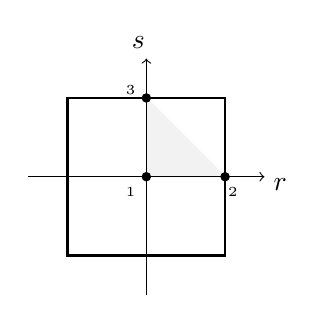
\begin{tikzpicture}
%\draw[step=0.5cm,gray,very thin] (0,0) grid (4,4); 
\draw[fill=gray!10,gray!10](2,2)--(3,2)--(2,3)--cycle;
\draw[thick] (1,1)--(3,1)--(3,3)--(1,3)--cycle;
\draw [->] (0.5,2) -- (3.5,2);
\draw [->] (2,0.5) -- (2,3.5);
\node[] at (3.7,1.9) {$r$};
\node[] at (1.9,3.7) {$s$};
\draw[black,fill=black] (2,2)   circle (1.5pt);
\draw[black,fill=black] (3,2)   circle (1.5pt);
\draw[black,fill=black] (2,3)   circle (1.5pt);
\node[] at (1.8,1.8) {\tiny $1$};
\node[] at (3.1,1.8) {\tiny $2$};
\node[] at (1.8,3.1) {\tiny $3$};
\end{tikzpicture}
\end{center}



and we would then have
\begin{mdframed}[backgroundcolor=blue!5]
\begin{eqnarray}
\bN_1(r) &=& 1-r-s  \nonumber\\
\bN_2(r) &=& r   \nonumber\\
\bN_3(r) &=& s
\end{eqnarray}
\end{mdframed}








%.....................................................................
\subsubsection{Enriched linear basis functions in triangles ($P_1^+$)}
\index{general}{$P_1^+$}

As we will see in Section~\ref{pair:mini} the above $P_1$ can be enriched 
with a so-called bubble function.
The \index{general}{Bubble Function} bubble function of the MINI element 
is described in \cite{arbf84} as being $\lambda_1\lambda_2\lambda_3$
where $\lambda_i$ are the so-called barycentric 
coordinates\footnote{\url{https://en.wikipedia.org/wiki/Barycentric\_coordinate\_system }}.
\index{general}{Barycentric Coordinates}

\begin{eqnarray}
\lambda_1 &=& \frac{(y2-y3)(x-x3)+(x3-x2)(y-y3)}{(y2-y3)(x1-x3)+(x3-x2)(y1-y3)} \nn\\
\lambda_2 &=& \frac{(y3-y1)(x-x3)+(x1-x3)(y-y3)}{(y2-y3)(x1-x3)+(x3-x2)(y1-y3)} \nn\\
\lambda_3 &=& 1-\lambda_1-\lambda_2 \nn
\end{eqnarray}

\begin{center}
\includegraphics[width=12cm]{images/mini/minielement2}\\
{\small representation of the element in the real coordinate system $(x,y)$
and in the reduced coordinate system $(r,s)$}
\end{center}

\begin{center}
\includegraphics[width=5cm]{images/mini/barycoord}\\
{\small Barycentric coordinates ($\lambda _{1},\lambda _{2},\lambda _{3}$) on an equilateral triangle and on a right triangle.}
\end{center}

In the reference triangle, the barycentric coordinates write
\begin{eqnarray}
\lambda_1 &=& \frac{(s_2-s_3)(r-r_3)+(r_3-r_2)(s-s_3)}{(s_2-s_3)(r_1-r_3)+(r_3-r_2)(s_1-s_3)} = \frac{(-1)(r)+(-1)(s-1)}{(-1)(0)+(-1)(-1)} = -r-s+1  \nn\\
\lambda_2 &=& \frac{(s3-s1)(r-r3)+(r1-r3)(s-s3)}{(s2-s3)(r1-r3)+(r3-r2)(s1-s3)} = \frac{(1)(r)+(0)(s-1)}{(-1)(0)+(-1)(-1)} = r \nn\\
\lambda_3 &=& 1-\lambda_1-\lambda_2 = 1 - (-r-s+1) - r = s \nn
\end{eqnarray}
As we have seen before the bubble function is given by $\lambda_1\lambda_2\lambda_3 = (1-r-s)rs$
and the polynomial form for the basis functions is given by:
\[
f(r,s) =a+br+cs + d (1-r-s)rs
\]
Setting the location of the bubble at $r=s=1/3$, i.e. $\lambda_1\lambda_2\lambda_3 = 1/3$, 
we then have 
\begin{eqnarray}
f(r_1,s_1)&=&f_1 = a+br_1+cs_1 + d (1-r_1-s_1)r_1s_1 = a \nn\\
f(r_2,s_2)&=&f_2 = a+br_2+cs_2 + d (1-r_2-s_2)r_2s_2 = a + b \nn\\
f(r_3,s_3)&=&f_3 = a+br_3+cs_3 + d (1-r_3-s_3)r_3s_3 = a + c \nn\\
f(r_4,s_4)&=&f_4 = a+br_4+cs_4 + d (1-r_4-s_4)r_4s_4 = a + \frac{b}{3} + \frac{c}{3} + \frac{1}{27} \nn
\end{eqnarray}
where point 4 is the location of the bubble.
This yields
\[
a=f_1 
\quad\quad\qquad
b=f_2-a = f_2-f_1
\quad\quad\qquad
c=f_3-a = f_3-f_1
\]
and
\[
d=27(f_4-a-\frac{b}{3} - \frac{c}{3}) = 27 (f_4 - f_1 - \frac{f_2-f_1}{3} - \frac{f_3-f_1}{3} )
=27(f_4 - \frac{f_1}{3}  - \frac{f_2}{3}  - \frac{f_3}{3} )
\] 

Finally
\begin{eqnarray}
f(r,s) 
&=&a+br+cs + d (1-r-s)rs \nn\\
&=& f_1 + (f_2-f_1)r + (f_3-f_1)s + 27(f_4 - \frac{f_1}{3}  - \frac{f_2}{3}  - \frac{f_3}{3} ) (1-r-s)rs \nn\\
&=& [1-r-s-9(1-r-s)rs] f_1 + [r-9(1-r-s)rs ]f_2 + [s-9(1-r-s)rs ]f_3 + [27(1-r-s)rs]f_4 \nn
\end{eqnarray}
so that 
\[
f(r,s)=\sum_{i=1}^4 N_i(r,s) f_i
\]
with 
%\begin{mdframed}[backgroundcolor=blue!15]
\begin{eqnarray}
N_1(r,s) &=& 1-r-s-9(1-r-s)rs \nn\\
N_2(r,s) &=& r-9(1-r-s)rs \nn\\
N_3(r,s) &=& s-9(1-r-s)rs \nn\\
N_4(r,s) &=& 27(1-r-s)rs \nn
\end{eqnarray}
%\end{mdframed}
It is trivial to verify that $\sum_i N_i =1$ for all values of $r,s$
and the gradients of the basis functions are:
\begin{eqnarray}
\frac{\partial N_1}{\partial r}(r,s) &=& -1 - 9(1-2r-s)s \\ 
\frac{\partial N_2}{\partial r}(r,s) &=&  +1 - 9(1-2r-s)s \\ 
\frac{\partial N_3}{\partial r}(r,s) &=&  - 9(1-2r-s)s \\ 
\frac{\partial N_4}{\partial r}(r,s) &=&  27(1-2r-s)s \\ 
\\
\frac{\partial N_1}{\partial s}(r,s) &=& -1 - 9(1-r-2s)r \\ 
\frac{\partial N_2}{\partial s}(r,s) &=&    - 9(1-r-2s)r \\ 
\frac{\partial N_3}{\partial s}(r,s) &=& +1 - 9(1-r-2s)r \\ 
\frac{\partial N_4}{\partial s}(r,s) &=&     27(1-r-2s)r 
\end{eqnarray}

We have two coordinate systems for the element: the global coordinates $(x,y)$ 
and the natural coordinates $(r,s)$. Inside the element, the relation between the two is given by
\begin{eqnarray}
x &=& N_1 x_1 + N_2 x_2 + N_3 x_3 + N_4 x_4 = \sum_i N_i(r,s) x_i\nn\\
y &=& N_1 y_1 + N_2 y_2 + N_3 y_3 + N_4 y_4 = \sum_i N_i(r,s) y_i
\end{eqnarray}
or,
\begin{eqnarray}
x &=& [ 1-r-s-9(1-r-s)rs] x_1 + [r-9(1-r-s)rs] x_2 + [s-9(1-r-s)rs] x_3 + [27(1-r-s)rs] x_4 \nn\\
&=& x_1 -r (x_1-x_2) -s (x_1-x_3) + (1-r-s)rs (-9 x_1 - 9 x_2  -9 x_3 +27 x_4)  \nn\\
&=& x_1 -r (x_1-x_2) -s (x_1-x_3) + (1-r-s)rs (-9 x_1 - 9 x_2  -9 x_3 +27 (x_1+x_2+x_3)/3) \nn\\ 
&=& x_1 -r (x_1-x_2) -s (x_1-x_3) \nn\\ 
&=& x_1 -r x_{12} -s x_{13} \nn\\ 
y &=& [ 1-r-s-9(1-r-s)rs] y_1 + [r-9(1-r-s)rs] y_2 + [s-9(1-r-s)rs] y_3 + [27(1-r-s)rs] y_4 \nn\\
&=& y_1 -r (y_1-y_2) -s (y_1-y_3) + (1-r-s)rs (-9 y_1 - 9 y_2  -9 y_3 +27 y_4)  \nn\\
&=& y_1 -r (y_1-y_2) -s (y_1-y_3) + (1-r-s)rs (-9 y_1 - 9 y_2  -9 y_3 +27 (y_1+y_2+y_3)/3) \nn\\ 
&=& y_1 -r (y_1-y_2) -s (y_1-y_3) \nn \\
&=& y_1 -r y_{12} -s y_{13} \nn 
\end{eqnarray}




























%%%%%%%%%%%%%%%%%%%%%%%%%%%%%%%%%%%%
\subsubsection{Quadratic basis functions for triangles in 2D ($P_2$)}
\index{general}{$P_2$}

\begin{verbatim}
2            
|\
| \        (r_0,s_0)=(0,0) (r_3,s_3)=(1/2,0)
5   4      (r_1,s_1)=(1,0) (r_4,s_4)=(1/2,1/2)
|     \    (r_2,s_2)=(0,1) (r_5,s_5)=(0,1/2)
|      \ 
0===3===1
\end{verbatim}
The basis polynomial is then
\[
f(r,s) = c_1 + c_2 r + c_3 s + c_4  r^2 + c_5 rs  + c_6 s^2
\]
We have 
\begin{eqnarray}
f_1 = f(r_1,s_1) &=& c_1 \nonumber\\
f_2 = f(r_2,s_2) &=& c_1 + c_2 + c_4\nonumber\\
f_3 = f(r_3,s_3) &=& c_1 + c_3 + c_6\nonumber\\
f_4 = f(r_4,s_4) &=& c_1 + c_2/2 + c_4/4\nonumber\\
f_5 = f(r_5,s_5) &=& c_1 + c_2/2 + c_3/2 \nonumber\\
                 &+& c_4/4 + c_5/4 + c_6/4\nonumber\\
f_6 = f(r_6,s_6) &=& c_1 + c_3/2 + c_6/4\nonumber
\end{eqnarray}

This can be cast as ${\bm f}={\bm A}\cdot {\bm c}$ where ${\bm A}$ is a 6x6 matrix:
\[
{\bm A}=
\left(
\begin{array}{cccccc}
1&0   &  0  & 0   & 0   & 0\\
1&1   &  0  & 1   & 0   & 0\\
1&0   &  1  & 0   & 0   & 1\\
1&1/2 &  0  & 1/4 & 0   & 0\\
1&1/2 &  1/2& 1/4 & 1/4 & 1/4\\
1&0   &  1/2& 0   & 0   & 1/4
\end{array}
\right)
\]
It is rather trivial to compute the inverse of this matrix:
\[
{\bm A}^{-1}=
\left(
\begin{array}{cccccc}
1  & 0 & 0  & 0  & 0 & 0  \\
-3 & -1& 0  & 4  & 0 & 0 \\
-3 & 0 & -1 & 0  & 0 & 4 \\
2  & 2 & 0  & -4 & 0 & 0  \\
4  & 0 & 0  & -4 & 4 & -4 \\
2  & 0 & 2  & 0  & 0 & -4
\end{array}
\right)
\]
In the end, one obtains:
\begin{eqnarray}
f(r,s) 
&=& f_1 + (-3f_1-f_2+4f_4) r + (-3f_1-f_3+4f_6)s \nonumber\\
&& +(2f_1+2f_2-4f_4)r^2 + (4f_1-4f_4+4f_5-4f_6) rs \nn\\
&&+ (2f_1+2f_3-4f_6)s^2 \nonumber\\
&=& \sum_{i=1}^6 N_i(r,s) f_i
\end{eqnarray}
with
\begin{mdframed}[backgroundcolor=blue!5]
\begin{eqnarray}
N_1(r,s) &=& 1-3r-3s+2r^2+4rs+2s^2 \nonumber\\
N_2(r,s) &=& -r+2r^2 \nonumber\\
N_3(r,s) &=& -s+2s^2 \nonumber\\
N_4(r,s) &=& 4r-4r^2-4rs \nonumber\\
N_5(r,s) &=& 4rs \nonumber\\
N_6(r,s) &=& 4s-4rs-4s^2 \nonumber
\end{eqnarray}
\end{mdframed}

The derivatives are as follows:
\begin{eqnarray}
\frac{\partial N_1}{\partial r}(r,s) &=&  -3+4r+4s \nn\\ 
\frac{\partial N_2}{\partial r}(r,s) &=&  -1+4r\nn\\ 
\frac{\partial N_3}{\partial r}(r,s) &=&  0\nn\\ 
\frac{\partial N_4}{\partial r}(r,s) &=&  4-8r-4s\nn\\ 
\frac{\partial N_5}{\partial r}(r,s) &=&  4s\nn\\ 
\frac{\partial N_6}{\partial r}(r,s) &=&  -4s\nn
\end{eqnarray}

\begin{eqnarray}
\frac{\partial N_1}{\partial s}(r,s) &=&  -3+4r+4s\nn\\ 
\frac{\partial N_2}{\partial s}(r,s) &=&  0\nn\\ 
\frac{\partial N_3}{\partial s}(r,s) &=&  -1+4s\nn\\ 
\frac{\partial N_4}{\partial s}(r,s) &=&  -4r\nn\\ 
\frac{\partial N_5}{\partial s}(r,s) &=&  4r\nn\\ 
\frac{\partial N_6}{\partial s}(r,s) &=&  4-4r-8s\nn
\end{eqnarray}



%.....................................................................
\subsubsection{Enriched quadratic basis functions in triangles ($P_2^+$)}
\index{general}{$P_2^+$}

This is used by the Crouzeix-Raviart element, see Section~\ref{sec:crouzeix-raviart}. 
\index{general}{Crouzeix-Raviart}

\begin{verbatim}
03             (r_1,s_1)=(0,0)
||\\           (r_2,s_2)=(1,0)
|| \\          (r_3,s_3)=(0,1)
||  \\         (r_4,s_4)=(1/2,0)
06   05        (r_5,s_5)=(1/2,1/2)
|| 07 \\       (r_6,s_6)=(0,1/2)
||     \\      (r_7,s_7)=(1/3,1/3)
01==04==02    
\end{verbatim}

The basis functions are given by:
\todo[inline]{find reference}

\begin{mdframed}[backgroundcolor=blue!5]
\begin{eqnarray}
N_1(r,s) &=&  (1-r-s)(1-2r-2s+ 3rs) \\
N_2(r,s) &=& r (2 r -1 + 3s-3rs-3s^2 ) \\
N_3(r,s) &=& s (2s -1 + 3r-3r^2-3rs )\\
N_4(r,s) &=& 4(1-r-s)r(1 -3s ) \\
N_5(r,s) &=& 4rs [-2+3r+3s]\\
N_6(r,s) &=& 4(1-r-s)s(1-3r)\\
N_7(r,s) &=& 27 (1-r-s)rs 
\end{eqnarray}
\end{mdframed}
It is then easy to verify that for all basis functions we have 
$N_i(r_j,s_j)=\delta_{ij}$ where $j$ denotes one of the seven nodes. 

The derivatives are as follows:
\begin{eqnarray}
\frac{\partial N_1}{\partial r}(r,s) &=& r(4-6s)-3s^2+7s-3\\
\frac{\partial N_2}{\partial r}(r,s) &=& r(4-6s)-3s^2+3s-1\\
\frac{\partial N_3}{\partial r}(r,s) &=& -3s(2r+s-1)  \\
\frac{\partial N_4}{\partial r}(r,s) &=& 4(3s-1)(2r+s-1) \\
\frac{\partial N_5}{\partial r}(r,s) &=& 4s(6r+3s-2) \\
\frac{\partial N_6}{\partial r}(r,s) &=& 4s(6r+3s-4)\\
\frac{\partial N_7}{\partial r}(r,s) &=& -27s(2r+s-1)
\end{eqnarray}

\begin{eqnarray}
\frac{\partial N_1}{\partial s}(r,s) &=& -3r^2+r(7-6s)+4s-3\\
\frac{\partial N_2}{\partial s}(r,s) &=& -3r(r+2s-1)\\
\frac{\partial N_3}{\partial s}(r,s) &=& -3r^2+r(3-6s)+4s-1 \\
\frac{\partial N_4}{\partial s}(r,s) &=& 4r(3r+6s-4)  \\
\frac{\partial N_5}{\partial s}(r,s) &=& 4r(3r+6s-2) \\
\frac{\partial N_6}{\partial s}(r,s) &=& 4(3r-1)(r+2s-1)\\
\frac{\partial N_7}{\partial s}(r,s) &=& -27r(r+2s-1)
\end{eqnarray}


Note that the basis functions can also be expressed as a function of the barycentric coordinates, 
as in the MILAMIN code \cite{daks08} or in Cuvelier \etal, 1986 \cite{cuss86}\footnote{Note
that the numbering of the nodes in the book is different with respect to the one above. }

\begin{verbatim}
03          
||\\        
|| \\       
||  \\      
05   04     
|| 07 \\    
||     \\   
01==06==02    
\end{verbatim}

\begin{eqnarray}
N_1(\lambda_1,\lambda_2,\lambda_3) &=& \eta_1(2\eta_1-1)+ 3\eta_1\eta_2\eta_3\\
N_2(\lambda_1,\lambda_2,\lambda_3) &=& \eta_2(2\eta_2-1)+ 3\eta_1\eta_2\eta_3\\
N_3(\lambda_1,\lambda_2,\lambda_3) &=& \eta_3(2\eta_3-1)+ 3\eta_1\eta_2\eta_3\\
N_4(\lambda_1,\lambda_2,\lambda_3) &=& 4\eta_2\eta_3 - 12\eta_1\eta_2\eta_3\\
N_5(\lambda_1,\lambda_2,\lambda_3) &=& 4\eta_1\eta_3 - 12\eta_1\eta_2\eta_3\\
N_6(\lambda_1,\lambda_2,\lambda_3) &=& 4\eta_1\eta_2 - 12\eta_1\eta_2\eta_3\\
N_7(\lambda_1,\lambda_2,\lambda_3) &=& 27\eta_1\eta_2\eta_3 
\end{eqnarray}

\todo[inline]{
VERIFY that when $\eta_1=1-r-s$, $\eta_2=r$ and $\eta_3=s$ we find the above $r,s$ basis functions
}


%1-4*eta1+3*eta1*eta3-3*eta2*eta3 ...
%-1+4*eta2+3*eta1*eta3-3*eta2*eta3 ...
%3*eta1*eta3-3*eta2*eta3 ...
%4*eta3+12*eta2*eta3-12*eta1*eta3 ...
%-4*eta3+12*eta2*eta3-12*eta1*eta3 ...
%4*eta1-4*eta2+12*eta2*eta3-12*eta1*eta3 ...
%-27*eta2*eta3+27*eta1*eta3

%1-4*eta1+3*eta1*eta2-3*eta2*eta3 ...
%+3*eta1*eta2-3*eta2*eta3 ...
%-1+4*eta3+3*eta1*eta2-3*eta2*eta3 ...
%4*eta2-12*eta1*eta2+12*eta2*eta3 ...
%4*eta1-4*eta3-12*eta1*eta2+12*eta2*eta3 ...
%-4*eta2-12*eta1*eta2+12*eta2*eta3 ...
%27*eta1*eta2-27*eta2*eta3];  







%%%%%%%%%%%%%%%%%%%%%%%%%%%%%%%%%%%%
\subsubsection{Cubic basis functions for triangles ($P_3$)}
\index{general}{$P_3$}

\begin{verbatim}
2
|\          (r_0,s_0)=(0,0)   (r_5,s_5)=(2/3,1/3)
|  \        (r_1,s_1)=(1,0)   (r_6,s_6)=(1/3,2/3)
7   6       (r_2,s_2)=(0,1)   (r_7,s_7)=(0,2/3)
|    \      (r_3,s_3)=(1/3,0) (r_8,s_8)=(0,1/3)
8  9   5    (r_4,s_4)=(2/3,0) (r_9,s_9)=(1/3,1/3)
|       \ 
0==3==4==1
\end{verbatim}
The basis polynomial is then
\[
f(r,s) = c_1 + c_2r + c_3s + c_4 r^2 + c_5 rs + c_6 s^2 + c_7 r^3 +c_8 r^2s + c_9 rs^2 + c_{10}s^3
\]
\begin{eqnarray}
N_0(r,s) &=& \frac{9}{2}(1-r-s)\left(\frac13-r-s\right)\left(\frac23-r-s\right) \\
N_1(r,s) &=& \frac{9}{2}r\left(r-\frac13\right)\left(r-\frac23 \right) \\
N_2(r,s) &=& \frac{9}{2}s\left(s-\frac13\right)\left(s-\frac23\right) \\
N_3(r,s) &=& \frac{27}{2}(1-r-s)r \left(\frac23-r-s\right) \\
N_4(r,s) &=& \frac{27}{2}(1-r-s)r\left(r-\frac13\right) \\
N_5(r,s) &=& \frac{27}{2}rs\left(r-\frac13\right) \\
N_6(r,s) &=& \frac{27}{2}rs\left(r-\frac23\right) \\
N_7(r,s) &=& \frac{27}{2}(1-r-s)s\left(s-\frac13\right) \\
N_8(r,s) &=& \frac{27}{2}(1-r-s)s \left(\frac23-r-s\right) \\
N_9(r,s) &=& 27 rs(1-r-s)
\end{eqnarray}



%..........................................................................
\subsubsection{Enriched linear basis functions in quadrilaterals ($Q_1^+$) -WIP} \label{ss:quadmini}
\index{general}{$Q_1^+$}

\begin{verbatim}
4===========3
|           |   (r_1,s_1)=(-1,-1)
|           |   (r_2,s_2)=(1,-1)
|     5     |   (r_3,s_3)=(1,1)
|           |   (r_4,s_4)=(-1,1)
|           |   (r_5,s_5)=(0,0)
1===========2
\end{verbatim}

\begin{itemize}
\item 
In Bai (1997) \cite{bai97}: "It is well known that the equal-order bilinear velocity-bilinear 
continuous pressure element - the $Q_1\times Q_1$, element - exhibits a certain spurious pressure mode.
In the paper we propose a new stabilized $Q_1\times Q_1$ combination for the velocity and
pressure with three internal degrees of freedom added to the velocity space, that is, one degree of
freedom for each component of the velocity and one degree of freedom shared by both components of
the velocity."

Two versions are proposed, if I understand it correctly.
The first one is given in Eq.~7 (three extra dofs: $u_5$, $v_5$, $w$):
\begin{eqnarray}
u^h(r,s) &=& \sum_{i=1}^4 N_i (r,s) u_i + \left[ u_5 - \frac{w}{4}(1-s) \right] (1-r^2)(1-s^2) \nonumber\\
v^h(r,s) &=& \sum_{i=1}^4 N_i (r,s) v_i + \left[ v_5 - \frac{w}{4}(1-r) \right] (1-r^2)(1-s^2) 
\end{eqnarray}
The second one in Eq.23 (four extra dofs: $u_5$, $v_5$, $u_6$, $v_6$):
\begin{eqnarray}
u^h(r,s) &=& \sum_{i=1}^4 N_i (r,s) u_i + \left[ u_5 +u_6(r+s) \right] (1-r^2)(1-s^2) \nonumber\\
v^h(r,s) &=& \sum_{i=1}^4 N_i (r,s) v_i + \left[ v_5 +v_6(r+s) \right] (1-r^2)(1-s^2) 
\end{eqnarray}

\item In Franca \etal (2007) \cite{fros07}: 
"Stabilized finite element method for Stokes equations with piecewise continuous 
bilinear approximations for both velocity and pressure variables. The velocity
field is enriched with piecewise polynomial bubble functions with null average at element
edges."

It looks like they are proposing (see their Eq.~2.6):
\begin{eqnarray}
u^h(r,s) &=& \sum_{i=1}^4 N_i (r,s) u_i + (\alpha + \gamma s)\frac{1}{2}(r^2+s^2-\frac43) \nn\\ 
v^h(r,s) &=& \sum_{i=1}^4 N_i (r,s) v_i + (\beta + \gamma r) \frac{1}{2}(r^2+s^2-\frac43)  
\end{eqnarray}

\item In Kwon \& Park \cite{kwpa14}: 
"We introduce a new stable MINI-element pair for incompressible Stokes equations on
quadrilateral meshes, which uses the smallest number of bubbles for the velocity. The pressure is 
discretized with the $P_1$-midpoint-edge-continuous elements and each component of the velocity field is
done with the standard $Q_1$-conforming elements enriched by one bubble a quadrilateral."

\item  In Lamichhane (2017) \cite{lami17}: "We consider a quadrilateral MINI
finite element for approximating the solution
of Stokes equations using a quadrilateral mesh. We use the standard bilinear finite
element space enriched with element-wise defined bubble functions for the velocity
and the standard bilinear finite element space for the pressure space. With a simple
modification of the standard bubble function we show that a single bubble function is
sufficient to ensure the inf-sup condition.
This is a refinement of \cite{bai97} where the author enriches the velocity space with
more than a single vector bubble function per element. In this article we show that 
with a small modification of the standard bubble function we can get the stability just 
by using a single vector bubble function per element."

\input{lamichhane2D}

\end{itemize}


\Literature Mons \& Roge (1992) \cite{moro92}, 
Li \etal (2009) \cite{lihc09}, Knobloch \& Tobiska (2000) \cite{knto00}, 
Franca \etal (1993) \cite{frha93}, Idelsohn \etal (1995) \cite{idsn95}.





\newpage
%-----------------------------------------------------------------
\subsubsection{The rotated $Q_1$} \label{ss:rq1}
\index{general}{$\tilde{Q}_1$}

The nodes are not on the corners of the element but in the middle of the
element edges:

\begin{flushright} {\tiny {\color{gray} (tikz\_RTQ1P0.tex)}} \end{flushright}
%~~~~~~~~~~~~~~~~~~~~~~~~~~~~~~~~~~~~~~~~~~~~~~~~~~~~~~~~~~~~~~~~~~~~~~~~~~~~~~~~~~~~~~~~~~~~~~~~~~

\begin{center}
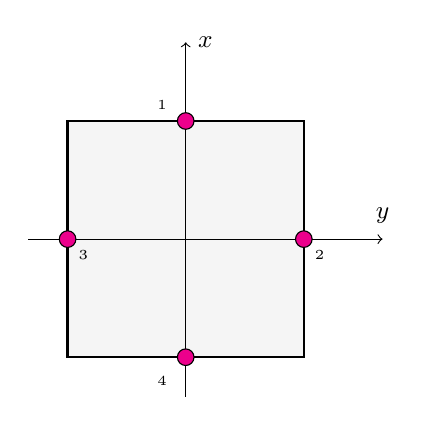
\begin{tikzpicture}
%\draw[step=1cm,gray,very thin] (0,0) grid (8,8); %background grid

\draw[thick,fill=gray!8] (1,1) -- (4,1) -- (4,4) -- (1,4) -- cycle;

\node[] at (1.2,2.3) {\tiny 3};
\node[] at (4.2,2.3) {\tiny 2};
\node[] at (2.2,.7) {\tiny 4};
\node[] at (2.2,4.2) {\tiny 1};

\draw[->] (0.5,2.5)--(5,2.5);
\draw[->] (2.5,0.5)--(2.5,5);

\draw[black,fill=magenta] (1,2.5)   circle (3pt);
\draw[black,fill=magenta] (4,2.5)   circle (3pt);
\draw[black,fill=magenta] (2.5,1)   circle (3pt);
\draw[black,fill=magenta] (2.5,4)   circle (3pt);

\node[] at (5,2.8) {\small $y$};
\node[] at (2.75,5) {\small $x$};
\end{tikzpicture}
\end{center}




\begin{verbatim}
+======3======+
|             |
|      s      |
|      |      |
4      +--r   2
|             |
|             |
|             |
+======1======+
\end{verbatim}

There are two types of basis functions: the Middle Point (MP) variant
such that $N_i({\bm r}_j)=\delta_{ij}$ and the Mid Value (MV) variant
such that $\frac{1}{|\Gamma_i|} \int_{\Gamma_i} N_j d\Gamma = \delta_{ij}$.

%.............................................
\paragraph{The Middle Point (MP) variant}. 
We have $\tilde{Q}_1=span \{ 1,r,s,r^2-s^2 \}$
so a function $f \in \tilde{Q}_1$  is such that 
\begin{equation}
f(r,s)= a + b r + c s + d(r^2-s^2 )
\label{nonpsf}
\end{equation}

This function must be so that 
\begin{eqnarray}
f_1 &=& f(r=0 ,s=-1) = a -c -d \\
f_2 &=& f(r=+1,s=0)  = a +b +d \\
f_3 &=& f(r=0 ,s=+1) = a +c -d \\
f_4 &=& f(r=-1,s=0)  = a -b +d 
\end{eqnarray}
and then 
\[
\left(
\begin{array}{c}
f_A \\ f_b \\ f_C \\ f_D
\end{array}
\right)
=
\left(
\begin{array}{cccc}
1 &0 &-1 &-1 \\
1 &1 &0 &1 \\
1 &0 &1 &-1 \\
1 &-1 &0 &1
\end{array}
\right)
\left(
\begin{array}{c}
a \\ b \\ c \\ d
\end{array}
\right)
\]
This system can easily be solved, $a,b,c,d$ are then replaced in Eq.~\eqref{nonpsf},
which yields 
\begin{eqnarray}
f(r,t) &=& N_1(r,s)f_1 +N_2(r,s)f_1 + N_3(r,s)f_3 +N_4(r,s)f_4
\end{eqnarray}
inside the element with
\begin{mdframed}[backgroundcolor=blue!5]
\begin{eqnarray}
N_1(r,s) &=& \frac{1}{4} (1-2s-(r^2-s^2)) \nonumber\\
N_2(r,s) &=& \frac{1}{4} (1+2r+(r^2-s^2)) \nonumber\\
N_3(r,s) &=& \frac{1}{4} (1+2s-(r^2-s^2)) \nonumber\\
N_4(r,s) &=& \frac{1}{4} (1-2r+(r^2-s^2)) \nonumber
\end{eqnarray}
\end{mdframed}
We of course recover the partition of unity property, i.e. $\sum N_i(r,s)=1$ for any coordinate $r,s$ inside 
the reference element.

\begin{remark}
These basis functions have been independently proposed by Donea \etal. \cite{dogm81}. The authors
prove herein that this element is checkerboard-free (although they do no show any example
of simulation carried out with this element).
\end{remark}

\begin{eqnarray}
\frac{\partial N_1}{\partial r} &=& \frac{1}{2}(-r)\\
\frac{\partial N_2}{\partial r} &=& \frac{1}{2}(1+r)\\
\frac{\partial N_3}{\partial r} &=& \frac{1}{2}(-r)\\
\frac{\partial N_4}{\partial r} &=& \frac{1}{2}(-1+r)
\end{eqnarray}

\begin{eqnarray}
\frac{\partial N_1}{\partial s} &=& \frac{1}{2}(-1+s)\\
\frac{\partial N_2}{\partial s} &=& \frac{1}{2}(-s)\\
\frac{\partial N_3}{\partial s} &=& \frac{1}{2}(1+s)\\
\frac{\partial N_4}{\partial s} &=& \frac{1}{2}(-s)
\end{eqnarray}

\begin{center}
\includegraphics[width=6cm]{images/rannacherturek/N1}
\includegraphics[width=6cm]{images/rannacherturek/N2}\\
\includegraphics[width=6cm]{images/rannacherturek/N3}
\includegraphics[width=6cm]{images/rannacherturek/N4}\\
{\captionfont Graphical representation of the $\tilde{Q}_1$ basis functions}
\end{center}

%......................................
\paragraph{The Mid Value (MV) variant}. 

These basis functions are implemented in deal.II
\footnote{\url{https://www.dealii.org/8.5.0/doxygen/deal.II/polynomials_rannacher_turek_8cc_source.html}}
for $x\in[0,1]$ and $y\in[0,1]$:

\begin{eqnarray}
N_1(x,y) &=&  0.75 + 1.5x - 2.5y -1.5(x^2-y^2) \quad bottom\\
N_2(x,y) &=& -0.25 - 0.5x + 1.5y +1.5(x^2-y^2) \quad right\\
N_3(x,y) &=& -0.25 + 1.5x - 0.5y -1.5(x^2-y^2) \quad top\\
N_4(x,y) &=&  0.75 - 2.5x + 1.5y +1.5(x^2-y^2) \quad left
\end{eqnarray}
We then proceed to rewrite these for $r\in[-1,1]$ and $t\in[-1:1]$:
\begin{mdframed}[backgroundcolor=blue!5]
\begin{eqnarray}
N_1(r,s) &=& \frac{1}{4} -\frac{1}{2}s - \frac{3}{8}(r^2-s^2) \quad bottom \\
N_2(r,s) &=& \frac{1}{4} +\frac{1}{2}r + \frac{3}{8}(r^2-s^2) \quad right \\
N_3(r,s) &=& \frac{1}{4} +\frac{1}{2}s - \frac{3}{8}(r^2-s^2) \quad top \\
N_4(r,s) &=& \frac{1}{4} -\frac{1}{2}r + \frac{3}{8}(r^2-s^2) \quad left
\end{eqnarray}
\end{mdframed}
It is easy to verify that these functions verify the property
\[
\frac{1}{|\Gamma_i|} \int_{\Gamma_i} N_j d\Gamma = \delta_{ij}
\]

These basis functions are used in \cite{shzh06} and mentioned in John \cite[p.722]{john16}.

\begin{eqnarray}
\frac{\partial N_1}{\partial r} &=& -\frac{3}{4}r \nonumber\\
\frac{\partial N_2}{\partial r} &=& \frac{1}{2}+\frac{3}{4}r \nonumber\\
\frac{\partial N_3}{\partial r} &=& -\frac{3}{4}r \nonumber\\
\frac{\partial N_4}{\partial r} &=& -\frac{1}{2}+\frac{3}{4}r \nonumber
\end{eqnarray}

\begin{eqnarray}
\frac{\partial N_1}{\partial t} &=& -\frac{1}{2}+\frac{3}{4}t \nonumber\\
\frac{\partial N_2}{\partial t} &=& -\frac{3}{4}t \nonumber\\
\frac{\partial N_3}{\partial t} &=& \frac{1}{2}+\frac{3}{4}t \nonumber\\
\frac{\partial N_4}{\partial t} &=& -\frac{3}{4}t \nonumber
\end{eqnarray}


\newpage
%-----------------------------------------------------------------------------
\subsubsection{The 2D enriched $Q_1^+\times P_0$ of Fortin} \label{ss:Q1pP02D}

We here consider the enriched $Q_1\times P_0$ element introduced first by 
Fortin (1981) \cite{fort81}.
The layout of the degrees of freedom is as follows:

\begin{flushright} {\tiny {\color{gray} (tikz\_q1pp02D.tex)}} \end{flushright}
%~~~~~~~~~~~~~~~~~~~~~~~~~~~~~~~~~~~~~~~~~~~~~~~~~~~~~~~~~~~~~~~~~~~~~~~~~~~~~~~~~~~~~~~~~~~~~~~~~~

\begin{center}
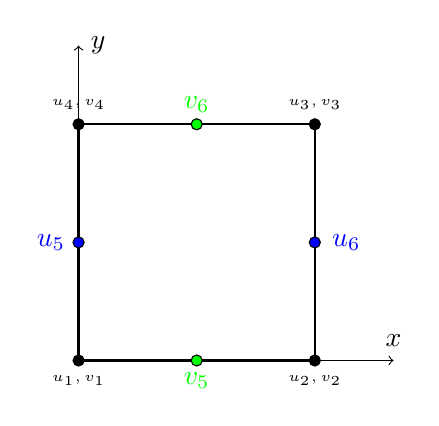
\begin{tikzpicture}
%\draw[fill=gray!23,gray!23](0,0) rectangle (6,5);
%\draw[step=0.5cm,gray,very thin] (0,0) grid (6,5); %background grid

\draw[thick] (1,.5) -- (4,.5) -- (4,3.5) -- (1,3.5) -- cycle; %front

\draw[thin,->] (4,0.5) -- (5,0.5); %x
\draw[thin,->] (1,3.5) -- (1,4.5); %y
\node[] at (5,0.75) {$x$};
\node[] at (1.25,4.5) {$y$};

\draw[black,fill=black] (1,.5)   circle (2pt);
\draw[black,fill=black] (4,.5)   circle (2pt);
\draw[black,fill=black] (4,3.5)   circle (2pt);
\draw[black,fill=black] (1,3.5)   circle (2pt);

\node[] at (1,0.25) {\tiny $u_1,v_1$};
\node[] at (4,0.25) {\tiny $u_2,v_2$};
\node[] at (4,3.75) {\tiny $u_3,v_3$};
\node[] at (1,3.75) {\tiny $u_4,v_4$};

\draw[black,fill=blue] (1,2) circle (2pt); 
\draw[black,fill=blue] (4,2) circle (2pt); 
\node[] at (0.65,2) {\color{blue} $u_5$};
\node[] at (4.4,2) {\color{blue} $u_{6}$};

\draw[black,fill=green] (2.5,0.5) circle (2pt); 
\draw[black,fill=green] (2.5,3.5) circle (2pt); 
\node[] at (2.5,0.25) {\color{green} $v_5$};
\node[] at (2.5,3.75) {\color{green} $v_{6}$};

\end{tikzpicture}\\
\end{center}


\noindent The approximation of the velocity components $u$ and $v$ inside the element is
\[
u^h(r,s) = a^u \; N_1(r,s) + b^u \;  N_2(r,s) + c^u \; N_3(r,s) +d^u \; N_4(r,s) 
+ d\; b_5^u(r,s) + e\; b_{6}^u(r,s)
\]
\[
v^h(r,s) = a^v \; N_1(r,s) + b^v \;  N_2(r,s) + c^v \; N_3(r,s) +d^v \; N_4(r,s) 
+ d^v b_5^v(r,s) + e^v b_{6}^v(r,s)
\]
where $N_{1,2,3,4}$ are the standard $Q_1$ basis functions in 2D and with 
\[
b_5^u(r,s) = \frac{1}{2}(1-r)(1-s^2)
\qquad
b_6^u(r,s) = \frac{1}{2}(1+r)(1-s^2)
\]
and
\[
b_5^v(r,s) = \frac{1}{2}(1-r^2)(1-s)
\qquad
b_6^v(r,s) = \frac{1}{2}(1-r^2)(1+s)
\]
In the end one arrives at

\begin{mdframed}[backgroundcolor=blue!5]
\begin{eqnarray}
{N}_1^u(r,s) &=&  N_1(r,s) - \frac{1}{2} b_5^u(r,s)\nn\\
{N}_2^u(r,s) &=&  N_2(r,s) - \frac{1}{2} b_6^u(r,s)\nn\\
{N}_3^u(r,s) &=&  N_3(r,s) - \frac{1}{2} b_6^u(r,s)\nn\\
{N}_4^u(r,s) &=&  N_4(r,s) - \frac{1}{2} b_5^u(r,s)\nn\\
{N}_5^u(r,s) &=&  b_5^u(r,s) \nn\\
{N}_6^u(r,s) &=&  b_6^u(r,s) \nn\\
\nn\\
{N}_1^v(r,s) &=&  N_1(r,s) - \frac{1}{2} b_5^v(r,s)\nn\\
{N}_2^v(r,s) &=&  N_2(r,s) - \frac{1}{2} b_5^v(r,s)\nn\\
{N}_3^v(r,s) &=&  N_3(r,s) - \frac{1}{2} b_6^v(r,s)\nn\\
{N}_4^v(r,s) &=&  N_4(r,s) - \frac{1}{2} b_6^v(r,s)\nn\\
{N}_5^v(r,s) &=&  b_5^v(r,s) \nn\\
{N}_6^v(r,s) &=&  b_6^v(r,s) 
\end{eqnarray}
\end{mdframed}

We can check for the zero-th order consistency: Let $u(r,s)=C$, then 
\begin{eqnarray}
u^h(r,s) 
= \sum_{i=1}^6 N_i^u(r,s) u_i 
= C \sum_{i=1}^6 N_i^u(r,s) 
= C \sum_{i=1}^4 N_i(r,s)  
= C
\end{eqnarray}



\newpage
%-----------------------------------------------------------------------------
\subsubsection{The DSSY element} \label{ss:dssy_2D}
This element is often reffered to as the 'DSSY' element becaus of the 
four authors of the original paper: Douglas, Santos, sheen and Ye (1999) \cite{doss99}.

The non-conforming finite element space i$Q_l$ is defined based on the 
reference square element on $[-1,1]^2$ :
\[
Q_l = \text{Span} \left\{ 1, r, s, \theta_l(r)-\theta_l(s)  \right\}
\qquad l=1,\; \text{or} \; 2
\]
with
\begin{eqnarray}
\theta_1(r)  &=& r^2-\frac53r^4  \nn\\
\theta_1'(r) &=& 2r-\frac{20}{3}r^3  \nn\\
\theta_2(r)  &=& r^2-\frac{25}{6} r^4 + \frac72 r^6 \\ 
\theta_2'(r) &=& 2r-\frac{50}{3} r^3 + 21 r^5
\end{eqnarray}
The dimension of $Q_l$ is four and the $\theta_l$ functions look like:
\begin{center}
\includegraphics[width=7cm]{images/dssy/theta1}
\includegraphics[width=7cm]{images/dssy/theta2}
\end{center}
We have:
\begin{itemize}
\item $\theta_1(r=-1)=\theta_1(r=+1)=-\frac23$, $\theta_1(r=0)=0$ 
\item $\theta_2(r=-1)=\theta_2(r=+1)=\frac13$, $\theta_2(r=0)=0$ 
\end{itemize}
The nodes are situated at the mid-edges of the quadrilateral:

\input{tikz_dssy2D}

The basis function corresponding to the node (1, 0) is given by
\begin{mdframed}[backgroundcolor=blue!5]
\begin{eqnarray}
N_1(r,s)^{(l)} &=& \frac{1}{4} - \frac{1}{2} r + \frac{\theta_l(r)-\theta_l(s)}{4 \theta_l(1)}  \nn\\
N_2(r,s)^{(l)} &=& \frac{1}{4} + \frac{1}{2} r + \frac{\theta_l(r)-\theta_l(s)}{4 \theta_l(1)}  \nn\\
N_3(r,s)^{(l)} &=& \frac{1}{4} - \frac{1}{2} s - \frac{\theta_l(r)-\theta_l(s)}{4 \theta_l(1)}  \nn\\
N_4(r,s)^{(l)} &=& \frac{1}{4} + \frac{1}{2} s - \frac{\theta_l(r)-\theta_l(s)}{4 \theta_l(1)}  
\end{eqnarray}
\end{mdframed}
We can easily verify that $\sum_i N_i(r,s,t)=1$ and that $N_i(\vec{r}_j)=\delta_{ij}$:
\begin{eqnarray}
N_1^{(l)}(r_1,s_1) 
&=& \frac{1}{4} -\frac{1}{2} (-1) + \frac{\theta_l(-1)-\theta_l(0)}{4 \theta_l(1)}  
= \frac{1}{4} +\frac{1}{2}  + \frac{\theta_l(-1)}{4 \theta_l(1)}  
= \frac{1}{4} +\frac{1}{2}  + \frac{1}{4}   = 1 \nn\\
N_1^{(l)}(r_2,s_2)
&=& \frac{1}{4} -\frac{1}{2} (+1) + \frac{\theta_l(+1)-\theta_l(0)}{4 \theta_l(1)}  
= \frac{1}{4} -\frac{1}{2} + \frac{\theta_l(+1)}{4 \theta_l(1)}  
= \frac{1}{4} -\frac{1}{2} + \frac{1}{4}   = 0 \nn\\
N_1^{(l)}(r_3,s_3)
&=& \frac{1}{4} -\frac{1}{2} (0) + \frac{\theta_l(0)-\theta_l(-1)}{4 \theta_l(1)}  
= \frac14 -\frac14  = 0 \nn\\
N_1^{(l)}(r_4,s_4)
&=& \frac{1}{4} -\frac{1}{2} (0) + \frac{\theta_l(0)-\theta_l(+1)}{4 \theta_l(1)}  
= \frac14 -\frac14  = 0 \nn\\
N_2^{(l)}(r_1,s_1) 
&=& \frac{1}{4} + \frac{1}{2} (-1) + \frac{\theta_l(-1)-\theta_l(0)}{4 \theta_l(1)}  
= \frac14 -\frac12 + \frac14 = 0 \nn\\
N_2^{(l)}(r_2,s_2)
&=& \frac{1}{4} + \frac{1}{2} (+1) + \frac{\theta_l(+1)-\theta_l(0)}{4 \theta_l(1)}  
= \frac14 + \frac12 + \frac14 =1 \nn\\
N_2^{(l)}(r_3,s_3)
&=& \frac{1}{4} + \frac{1}{2} (0) + \frac{\theta_l(0)-\theta_l(-1)}{4 \theta_l(1)}  
= \frac14 - \frac14 = 0 \nn\\
N_2^{(l)}(r_4,s_4)
&=& \frac{1}{4} + \frac{1}{2} (0) + \frac{\theta_l(0)-\theta_l(+1)}{4 \theta_l(1)}  
= \frac14 - \frac14 = 0 \nn\\
N_3^{(l)}(r_1,s_1)
&=& \frac{1}{4} - \frac{1}{2} (0) - \frac{\theta_l(-1)-\theta_l(0)}{4 \theta_l(1)} 
= \frac14 -\frac14 = 0\nn\\
N_3^{(l)}(r_2,s_2)
&=& \frac{1}{4} - \frac{1}{2} (0) - \frac{\theta_l(+1)-\theta_l(0)}{4 \theta_l(1)} 
= \frac14 -\frac14 = 0\nn\\
N_3^{(l)}(r_3,s_3)
&=& \frac{1}{4} - \frac{1}{2} (-1) - \frac{\theta_l(0)-\theta_l(-1)}{4 \theta_l(1)} 
= \frac14 +\frac12 + \frac14 = 1\nn\\
N_3^{(l)}(r_4,s_4)
&=& \frac{1}{4} - \frac{1}{2} (+1) - \frac{\theta_l(0)-\theta_l(+1)}{4 \theta_l(1)} 
= \frac14 -\frac12 + \frac14 = 0\nn\\
N_4^{(l)}(r_1,s_1)
&=& \frac{1}{4} + \frac{1}{2} (0) - \frac{\theta_l(-1)-\theta_l(0)}{4 \theta_l(1)}  
= \frac14 -\frac14 =0\nn\\
N_4^{(l)}(r_2,s_2)
&=& \frac{1}{4} + \frac{1}{2} (0) - \frac{\theta_l(+1)-\theta_l(0)}{4 \theta_l(1)}  
= \frac14 -\frac14 =0\nn\\
N_4^{(l)}(r_3,s_3)
&=& \frac{1}{4} + \frac{1}{2} (-1) - \frac{\theta_l(0)-\theta_l(-1)}{4 \theta_l(1)}  
= \frac14 -\frac12 +\frac14 = 0 \nn\\
N_4^{(l)}(r_4,s_4)
&=& \frac{1}{4} + \frac{1}{2} (1) - \frac{\theta_l(0)-\theta_l(1)}{4 \theta_l(1)}  
= \frac14 +\frac12 +\frac14 = 1 \nn
\end{eqnarray}

The basis functions can also be explicitely written for $\theta_1$ as in Cai \etal \cite{cady99}:
\begin{eqnarray}
N_1(r,s)^{(l)} 
&=& \frac{1}{4} - \frac{1}{2} r - \frac38 \left[\left( r^2-\frac53r^4 \right) - \left(s^2-\frac53s^4 \right) \right] \nn\\
N_2(r,s)^{(l)} 
&=& \frac{1}{4} + \frac{1}{2} r - \frac38 \left[\left( r^2-\frac53r^4 \right) - \left(s^2-\frac53s^4 \right) \right] \nn\\
N_3(r,s)^{(l)} 
&=& \frac{1}{4} - \frac{1}{2} s + \frac38 \left[\left( r^2-\frac53r^4 \right) - \left(s^2-\frac53s^4 \right) \right] \nn\\
N_4(r,s)^{(l)} 
&=& \frac{1}{4} + \frac{1}{2} s + \frac38 \left[\left( r^2-\frac53r^4 \right) - \left(s^2-\frac53s^4 \right) \right] 
\end{eqnarray}

The derivatives of the basis functions are as follows:
\begin{eqnarray}
\partial_r N_1(r,s)^{(l)} &=&  - \frac{1}{2}  + \frac{\theta_l'(r)}{4 \theta_l(1)}  \nn\\
\partial_r N_2(r,s)^{(l)} &=&  + \frac{1}{2}  + \frac{\theta_l'(r)}{4 \theta_l(1)}  \nn\\
\partial_r N_3(r,s)^{(l)} &=&  - \frac{\theta_l'(r)}{4 \theta_l(1)}  \nn\\
\partial_r N_4(r,s)^{(l)} &=&  - \frac{\theta_l'(r)}{4 \theta_l(1)}  
\end{eqnarray}

\begin{eqnarray}
\partial_s N_1(r,s)^{(l)} &=&   -\frac{\theta_l'(s)}{4 \theta_l(1)}  \nn\\
\partial_s N_2(r,s)^{(l)} &=&   -\frac{\theta_l'(s)}{4 \theta_l(1)}  \nn\\
\partial_s N_3(r,s)^{(l)} &=&   - \frac{1}{2} + \frac{\theta_l'(s)}{4 \theta_l(1)}  \nn\\
\partial_s N_4(r,s)^{(l)} &=&   + \frac{1}{2} + \frac{\theta_l'(s)}{4 \theta_l(1)}  
\end{eqnarray}





\Literature: 
Jeon \etal (2013) \cite{jens13},
Bangerth \etal (2017) \cite{baks17},
Sheen (2020) \cite{shee20}













 %-------------------------------
\subsection{Elements and basis functions in 3D} 

%%%%%%%%%%%%%%%%%%%%%%%%%%%%%%%%%%%%%%%%%%%%%%%%%%%%%%%
\subsubsection{Linear basis functions in tetrahedra ($P_1$)}
\index{$P_1$}


\begin{verbatim}
(r_0,s_0) = (0,0,0)
(r_1,s_1) = (1,0,0)
(r_2,s_2) = (0,2,0)
(r_3,s_3) = (0,0,1)
\end{verbatim}

The basis polynomial is given by
\[
f(r,s,t)=c_0 + c_1 r + c_2 s + c_3 t
\]

\begin{eqnarray}
f_1 &=& f(r_1,s_1,t_1) = c_0 \\
f_2 &=& f(r_2,s_2,t_2) = c_0 + c_1\\
f_3 &=& f(r_3,s_3,t_3) = c_0 + c_2\\
f_4 &=& f(r_4,s_4,t_4) = c_0 + c_3
\end{eqnarray}

which yields:
\[
c_0=f_1
\quad
\quad
c_1=f_2-f_1
\quad
\quad
c_2=f_3-f_1
\quad
\quad
c_3=f_4-f_1
\]

\begin{eqnarray}
f(r,s,t) 
&=& c_0 + c_1 r + c_2 s + c_3 t \nonumber\\
&=& f_1 + (f_2-f_1) r + (f_3-f_1) s + (f_4-f_1) t \nonumber\\
&=& f_1 (1-r-s-t) + f_2 r + f_3 s + f_4 t \nonumber\\
&=& \sum_i N_i(r,s,t) f_i \nonumber
\end{eqnarray}

Finally,

\begin{mdframed}[backgroundcolor=blue!5]
\begin{eqnarray}
N_1(r,s,t) &=& 1-r-s-t \nonumber\\
N_2(r,s,t) &=& r \nonumber\\
N_3(r,s,t) &=& s \nonumber\\
N_4(r,s,t) &=& t \nonumber
\end{eqnarray}
\end{mdframed}









%%%%%%%%%%%%%%%%%%%%%%%%%%%%%%%%%%%%%%%%%%%%%%%%%%%%%%%
\subsubsection{Triquadratic basis functions in 3D ($Q_2$)}
\index{$Q_2$}

\begin{eqnarray}
N_{1}&=& 0.5r(r-1)  \;0.5s(s-1)\; 0.5t(t-1)  \nonumber\\
N_{2}&=& 0.5r(r+1)  \;0.5s(s-1)\; 0.5t(t-1)  \nonumber\\
N_{3}&=& 0.5r(r+1)  \;0.5s(s+1)\; 0.5t(t-1)  \nonumber\\
N_{4}&=& 0.5r(r-1)  \;0.5s(s+1)\; 0.5t(t-1)  \nonumber\\
N_{5}&=& 0.5r(r-1)  \;0.5s(s-1)\; 0.5t(t+1)  \nonumber\\
N_{6}&=& 0.5r(r+1)  \;0.5s(s-1)\; 0.5t(t+1)  \nonumber\\
N_{7}&=& 0.5r(r+1)  \;0.5s(s+1)\; 0.5t(t+1)  \nonumber\\
N_{8}&=& 0.5r(r-1)  \;0.5s(s+1)\; 0.5t(t+1)  \nonumber\\
N_{9}&=& (1.-r^2)   \;0.5s(s-1)\; 0.5t(t-1)  \nonumber\\
N_{10}&=& 0.5r(r+1) \;(1-s^2)  \; 0.5t(t-1)  \nonumber\\
N_{11}&=& (1.-r^2)  \;0.5s(s+1)\; 0.5t(t-1)  \nonumber\\
N_{12}&=& 0.5r(r-1) \;(1-s^2)  \; 0.5t(t-1)  \nonumber\\
N_{13}&=& (1.-r^2)  \;0.5s(s-1)\; 0.5t(t+1)  \nonumber\\
N_{14}&=& 0.5r(r+1) \;(1-s^2)  \; 0.5t(t+1)  \nonumber\\
N_{15}&=& (1.-r^2)  \;0.5s(s+1)\; 0.5t(t+1)  \nonumber\\
N_{16}&=& 0.5r(r-1) \;(1-s^2)  \; 0.5t(t+1)  \nonumber\\
N_{17}&=& 0.5r(r-1) \;0.5s(s-1)\; (1-t^2)  \nonumber\\
N_{18}&=& 0.5r(r+1) \;0.5s(s-1)\; (1-t^2)  \nonumber\\
N_{19}&=& 0.5r(r+1) \;0.5s(s+1)\; (1-t^2)  \nonumber\\
N_{20}&=& 0.5r(r-1) \;0.5s(s+1)\; (1-t^2)  \nonumber\\
N_{21}&=& (1-r^2)   \;(1-s^2)  \; 0.5t(t-1)  \nonumber\\
N_{22}&=& (1-r^2)   \;0.5s(s-1)\; (1-t^2)  \nonumber\\
N_{23}&=& 0.5r(r+1) \;(1-s^2)  \; (1-t^2)  \nonumber\\
N_{24}&=& (1-r^2)   \;0.5s(s+1)\; (1-t^2)  \nonumber\\
N_{25}&=& 0.5r(r-1) \;(1-s^2)  \; (1-t^2)  \nonumber\\
N_{26}&=& (1-r^2)   \;(1-s^2)  \; 0.5t(t+1)  \nonumber\\
N_{27}&=& (1-r^2)   \;(1-s^2)  \; (1-t^2)  \nonumber
\end{eqnarray}

 %-------------------------------
%%%%%%%%%%%%%%%%%%%%%%%%%%%%%%%%%%%%%%%%%%%%%%%%%%%%%%%%%%%%%%%%%%%%%%%%%%%%%%%%%%%%%%%%%%%%%%%%%%%


\newpage 
%%%%%%%%%%%%%%%%%%%%%%%%%%%%%%%%%%%%%%%%%%%%%%%%%%%%%%%%%%%%%%%%%%%%%%%%%%%%%%%%%%%%%%%%%%%%%%%%%%%
\section{Solving the heat transport equation with linear Finite Elements} %%%%%%%%%%%%%%%%%%%%%%%%%
\subsection{The diffusion equation in 1D} \label{sec:diff1D} 
Let us consider the following one-dimensional grid: 
\begin{center}
\includegraphics[width=10cm]{images/oneD/domain}
\end{center}
Its spans the domain $\Omega$ of length $L_x$. 
It is discretised by means of 
$nnx$ nodes and $nelx=nnx-1$ elements.
Zooming in on element which is bounded by two nodes $k$ and $k+1$,
its size (also sometimes called diameter) is $h_x=x_{k+1}-x_k$, 
and the temperature field we wish to compute is located on those 
nodes so that they are logically called $T_k$ and $T_{k+1}$:

\begin{center}
\includegraphics[width=8cm]{images/oneD/el1D}
\end{center}

We focus here on the 1D diffusion equation (no advection, no heat sources):
\begin{equation}
\rho C_p \frac{\partial T}{\partial t} 
= \frac{\partial }{\partial x} \left( k \frac{\partial T}{\partial x}  \right)
\end{equation}
This is the {\color{olive}strong form} of the ODE to solve.
I can multiply this equation by a function\footnote{This function should be well-behaved with special properties, but we here assume it is a polynomial function.} $f(x)$ and integrate it over $\Omega$:
\begin{equation}
\int_{\Omega} f(x)  \rho C_p\frac{\partial T}{\partial t} dx
=
\int_{\Omega} f(x) \frac{\partial }{\partial x} \left( k \frac{\partial T}{\partial x}  \right) dx
\end{equation}
Looking at the right hand side, it is of the form $\int u v'$ so that I naturally 
integrate it by parts:
\begin{equation}
\int_{\Omega} f(x) \frac{\partial }{\partial x} 
\left( k \frac{\partial T}{\partial x}  \right) dx
=
\left[
f(x) k \frac{\partial T}{\partial x}
\right]_{\partial \Omega}
-
\int_{\Omega} \frac{\partial f}{\partial x}  k \frac{\partial T}{\partial x}  dx
\end{equation}
Assuming there is no heat flux prescribed on the boundary (i.e. $q_x= - k \partial T/\partial x = 0$ ),
\todo[inline]{NOT happy with this statement!!} then:
\begin{equation}
\int_{\Omega} f(x) \frac{\partial }{\partial x} \left( k \frac{\partial T}{\partial x}  \right) dx
=
- \int_{\Omega} \frac{\partial f}{\partial x}  k \frac{\partial T}{\partial x}  dx
\end{equation}
We then obtain the {\color{olive}weak form} of the diffusion equation in 1D:
\begin{equation}
\boxed{
\int_{\Omega} f(x) \rho C_p \frac{\partial T}{\partial t} dx
+
\int_{\Omega} \frac{\partial f}{\partial x}  k \frac{\partial T}{\partial x}  dx = 0
}
\end{equation}
We then use the additive property of the integral 
$\int_\Omega \dots = \sum_{elts} \int_{\Omega_e} \dots$
so that 
\begin{equation}
\sum_{elts} \left(     
\underbrace{ \int_{\Omega_e} f(x) \rho C_p   \frac{\partial T}{\partial t} dx }_{{\Lambda}_f^e}
+
\underbrace{\int_{\Omega_e} \frac{\partial f}{\partial x}  k \frac{\partial T}{\partial x}  dx}_{{\Upsilon}_f^e}      \right) = 0  
\end{equation}

In order to compute these integrals (analytically or by means of a numerical quadrature), 
we will need to evaluate $T$ inside the element. However, inside the element, 
the temperature is not known: all we have is the temperature at the nodes. 
For $x\in [x_k,x_{k+1}]$ we need to come up with a way to compute the temperature at this location. 
It makes sense to think that $T(x)$ will then be a function of the temperature at the nodes, 
i.e. $T(x) = \alpha T_k + \beta T_{k+1}$ where $\alpha$ and $\beta$ are coefficients. 
One over-simplified approach would be to assign $T(x)=(T_k + T_{k+1})/2$ but this would make the
temperature discontinuous from element to element. 
The rather logical solution to this problem is a linear temperature field between $T_k$
and $T_{k+1}$: 

\begin{eqnarray}
T(x) 
%&=& N_{k}(x) T_k + N_{k+1}(x) T_{k+1}  \nn\\
&=& \underbrace{\frac{x_{k+1}-x}{h_x}}_{N_k^\theta(x)} T_k 
+ 
\underbrace{\frac{x-x_k}{h_x}}_{N_{k+1}^\theta(x)} T_{k+1} \nn
\end{eqnarray}
where $N_k^\theta(x)$ is the (temperature) shape function associated to node $k$ and 
$N_{k+1}^\theta(x)$ is the shape function associated to node $k+1$.

Rather reassuringly, we have:
\begin{itemize}
\item $x=x_k$ yields $T(x)=T_k$
\item $x=x_{k+1}$ yields $T(x)=T_{k+1}$
\item $x=(x_k+x_{k+1})/2$ yields $T(x)=(T_k+T_{k+1})/2$
\end{itemize}
In what follows we abbreviate $\partial T/\partial x$ by $\dot{T}$.
Let us compute ${\Lambda}_f^e$ and ${\Upsilon}_f^e$ separately.
\begin{eqnarray}
{\Lambda}_f^e 
&=&\int_{x_k}^{x_{k+1}} f(x) \rho C_p \dot T(x) dx \nn\\
&=& \int_{x_k}^{x_{k+1}} f(x) \rho C_p \;\;  [ N_{k}^\theta(x) \dot{T}_k + N_{k+1}^\theta(x) \dot{T}_{k+1} ] \;\; dx  \nn\\
&=& \int_{x_k}^{x_{k+1}} f(x) \rho C_p N_{k}^\theta(x) \dot{T}_k  dx  
+ \int_{x_k}^{x_{k+1}} f(x) \rho C_p N_{k+1}^\theta(x) \dot{T}_{k+1}   dx \nn\\
&=&  \left( \int_{x_k}^{x_{k+1}} f(x) \rho C_p  N_{k}^\theta(x) dx \right) \dot{T}_k  
+ \left( \int_{x_k}^{x_{k+1}} f(x) \rho C_p N_{k+1}^\theta(x) dx \right)  \dot{T}_{k+1}  \nn
\end{eqnarray}
Taking $f(x)=N_k^\theta(x)$ and omitting '$(x)$' in the rhs:
\[
{\Lambda}_{N_k^\theta}^e=
%\int_{x_k}^{x_{k+1}} {\color{blue}f}(x) \rho C_p \dot{\color{blue}T}(x) dx
\left( \int_{x_k}^{x_{k+1}} \rho C_p  N_k^\theta N_{k}^\theta dx \right) \dot{T}_k  
+ \left( \int_{x_k}^{x_{k+1}} \rho C_p N_k^\theta N_{k+1}^\theta dx \right)  \dot{T}_{k+1} 
\]
Taking $f(x)=N_{k+1}^\theta(x)$ and omitting '$(x)$' in the rhs:
\[
{\Lambda}_{N_{k+1}^\theta}^e
%\int_{x_k}^{x_{k+1}} {\color{blue}f}(x) \dot{\color{blue}T}(x) dx
=  \left( \int_{x_k}^{x_{k+1}} \rho C_p N_{k+1}^\theta N_{k}^\theta dx \right) \dot{T}_k  
+ \left( \int_{x_k}^{x_{k+1}}  \rho C_p  N_{k+1}^\theta N_{k+1}^\theta dx \right)  \dot{T}_{k+1} 
\]
We can rearrange these last two equations as follows:
\[
\left(
\begin{array}{c}
{\Lambda}_{N_k^\theta}^e  \\ \\ {\Lambda}_{N_{k+1}^\theta}^e
\end{array}
\right)
=
\left(
\begin{array}{cc}
\int_{x_k}^{x_{k+1}} N_k^\theta     \rho C_p N_{k}^\theta dx  &  \int_{x_k}^{x_{k+1}} N_k^\theta  \rho C_p N_{k+1}^\theta dx \\ \\
\int_{x_k}^{x_{k+1}} N_{k+1}^\theta \rho C_p N_{k}^\theta dx  &  \int_{x_k}^{x_{k+1}} N_{k+1}^\theta \rho C_p N_{k+1}^\theta dx 
\end{array}
\right)
\cdot
\left(
\begin{array}{c}
\dot{T}_k \\ \\
\dot{T}_{k+1}
\end{array}
\right)
\]
and we can take the integrals outside of the matrix:
\[
\left(
\begin{array}{c}
{\Lambda}_{N_k^\theta}^e \\ \\ {\Lambda}_{N_{k+1}^\theta}^e
\end{array}
\right)
=
\left[
\int_{x_k}^{x_{k+1}}
\rho C_p
\left(
\begin{array}{cc}
N_k^\theta N_{k}^\theta     &  N_k^\theta N_{k+1}^\theta  \\ \\
N_{k+1}^\theta N_{k}^\theta &  N_{k+1}^\theta N_{k+1}^\theta 
\end{array}
\right)
dx
\right]
\cdot
\left(
\begin{array}{c}
\dot{T}_k \\ \\ 
\dot{T}_{k+1}
\end{array}
\right)
\]
Finally, we can define the vectors 
\[
{\vec N}^T = 
\left(
\begin{array}{c}
N_k^\theta(x)  \\ \\  N_{k+1}^\theta (x)
\end{array}
\right)
\]
and 
\[
{\vec T}^e = 
\left(
\begin{array}{c}
T_k \\ \\ T_{k+1}
\end{array}
\right)
\quad
\quad
\quad
\quad
\quad
\dot{\vec T}^e = 
\left(
\begin{array}{c}
\dot{T}_k \\ \\ \dot{T}_{k+1}
\end{array}
\right)
\]
so that 
\[
\left(
\begin{array}{c}
{\Lambda}_{N_k^\theta}^e \\  \\ {\Lambda}_{N_{k+1}^\theta}^e
\end{array}
\right)
=
\left( \int_{x_k}^{x_{k+1}}   {\vec N}^T \rho C_p  {\vec N} dx  \right) \cdot \dot{\vec T}^e
\]

Back to the diffusion term:

\begin{eqnarray}
{\Upsilon}_f^e &=&
\int_{x_k}^{x^{k+1}} \frac{\partial f}{\partial x} k \frac{\partial T}{\partial x} dx \nn\\
&=&
\int_{x_k}^{x^{k+1}} \frac{\partial f}{\partial x} k \frac{\partial  (N_{k}^\theta(x) T_k + N_{k+1}^\theta(x) T_{k+1} ) }{\partial x} dx  \nn\\
%&=&
%\int_{x_k}^{x^{k+1}} \left( \frac{\partial {\color{blue}f}}{\partial x}  \frac{\partial  {\color{blue}N}_{k} } {\partial x}  T_k 
%+ \frac{\partial {\color{blue}f}}{\partial x}  \frac{\partial  {\color{blue}N}_{k+1} } {\partial x}  T_{k+1} \right)  dx \nn\\
&=&
\left( \int_{x_k}^{x^{k+1}} \frac{\partial f}{\partial x}  k \frac{\partial  N_{k}^\theta } {\partial x}  dx \right)  T_k 
+ \left( \int_{x_k}^{x^{k+1}} \frac{\partial f}{\partial x}  k \frac{\partial  N_{k+1}^\theta } {\partial x} dx \right) T_{k+1}  \nn
\end{eqnarray}
Taking $f(x)=N_k^\theta(x)$ 
\[
{\Upsilon}_{N_k^\theta}^e=
%\int_{x_k}^{x^{k+1}} \frac{\partial {\color{blue}f}}{\partial x} \frac{\partial {\color{blue}T}}{\partial x} dx
\left( \int_{x_k}^{x^{k+1}} k\frac{\partial N_k^\theta}{\partial x}  \frac{\partial  N_{k}^\theta } {\partial x}  dx \right)  T_k 
+ \left( \int_{x_k}^{x^{k+1}} k \frac{\partial N_k^\theta}{\partial x}  \frac{\partial  N_{k+1}^\theta } {\partial x} dx \right) T_{k+1}  \nn
\]
Taking $f(x)=N_{k+1}^\theta(x)$ 
\[
{\Upsilon}_{N_{k+1}^\theta}^e=
%\int_{x_k}^{x^{k+1}} \frac{\partial {\color{blue}f}}{\partial x} \frac{\partial {\color{blue}T}}{\partial x} dx
%=
\left( \int_{x_k}^{x^{k+1}} k\frac{\partial N_{k+1}^\theta}{\partial x}  \frac{\partial  N_{k}^\theta } {\partial x}  dx \right)  T_k 
+ \left( \int_{x_k}^{x^{k+1}}  k\frac{\partial N_{k+1}^\theta}{\partial x}  \frac{\partial  N_{k+1}^\theta } {\partial x} dx \right) T_{k+1}  \nn
\]


\[
\left(
\begin{array}{cc}
 {\Upsilon}_{N_k^\theta}^e \\ \\ {\Upsilon}_{N_{k+1}^\theta}^e
\end{array}
\right)
=
\left(
\begin{array}{cc}
\int_{x_k}^{x^{k+1}} \frac{\partial N_k^\theta}{\partial x} k \frac{\partial  N_{k}^\theta } {\partial x}  dx & 
\int_{x_k}^{x^{k+1}} \frac{\partial N_k^\theta}{\partial x} k \frac{\partial  N_{k+1}^\theta } {\partial x} dx 
\\ \\
\int_{x_k}^{x^{k+1}} \frac{\partial N_{k+1}^\theta}{\partial x} k \frac{\partial  N_{k}^\theta } {\partial x}  dx & 
\int_{x_k}^{x^{k+1}} \frac{\partial N_{k+1}^\theta}{\partial x} k \frac{\partial  N_{k+1}^\theta } {\partial x} dx 
\end{array}
\right)
\cdot
\left(
\begin{array}{c}
T_k \\ \\ T_{k+1}
\end{array}
\right)
\]

or,
\[
\left(
\begin{array}{cc}
 {\Upsilon}_{N_k^\theta}^e \\ \\ {\Upsilon}_{N_{k+1}^\theta}^e
\end{array}
\right)
=
\left[
\int_{x_k}^{x^{k+1}}
k
\left(
\begin{array}{cc}
\frac{\partial N_k^\theta}{\partial x}  \frac{\partial  N_{k}^\theta } {\partial x}   & 
\frac{\partial N_k^\theta}{\partial x}  \frac{\partial  N_{k+1}^\theta } {\partial x}  
\\ \\
\frac{\partial N_{k+1}^\theta}{\partial x}  \frac{\partial  N_{k}^\theta } {\partial x}   & 
\frac{\partial N_{k+1}^\theta}{\partial x}  \frac{\partial  N_{k+1}^\theta } {\partial x}  
\end{array}
\right)
dx
\right]
\cdot
\left(
\begin{array}{c}
T_k \\ \\ T_{k+1}
\end{array}
\right)
\]
Finally, we can define the vector 
\[
{\vec B}^T=
\left(
\begin{array}{cc}
 \frac{\partial N_k^\theta}{\partial x}   \\ \\
 \frac{\partial N_{k+1}^\theta}{\partial x}
\end{array}
\right)
\]
so that 
\[
\left(
\begin{array}{cc}
 {\Upsilon}_{N_k^\theta}^e \\ \\ {\Upsilon}_{N_{k+1}^\theta}^e
\end{array}
\right)
=
\left( \int_{x_k}^{x_{k+1}}   {\vec B}^T k {\vec B} dx  \right) \cdot {\vec T}^e
\]

The weak form discretised over 1 element becomes
\[
\underbrace{\left( \int_{x_k}^{x_{k+1}}   {\vec N}^T \rho C_p {\vec N} dx  \right) }_{\bm M^e} \cdot \dot{\vec T}^e
+
\underbrace{\left( \int_{x_k}^{x_{k+1}}   {\vec B}^T k {\vec B} dx  \right)}_{{\bm K}_d^e} \cdot {\vec T}^e
=0
\]
or,
\[
\boxed{
{\bm M}^e \cdot \dot{\vec T}^e + {\bm K}_d^e \cdot {\vec T}^e = 0
}
\]
or,
\[
\boxed{
{\bm M}^e \cdot \frac{\partial {\vec T}^e}{\partial t} + {\bm K}_d^e \cdot {\vec T}^e = 0
}
\]
${\bm M}^e$ is commonly called the mass matrix, or capacitance matrix \cite[p103]{reddybook2}.
\index{Mass matrix}\index{Capacitance matrix}

Using a backward first order in time discretisation for the time derivative:
\[
\dot{\vec T}= \frac{\partial {\vec T}}{\partial t} = \frac{{\vec T}^{new}-{\vec T}^{old}}{\delta t}
\]
we get
\[
{\bm M}^e \cdot \frac{{\vec T}^{new}-{\vec T}^{old}}{\delta t} + {\bm K}_d^e \cdot {\vec T}^{new} = 0
\]
or, 
\[
\boxed{
( {\bm M}^e +  {\bm K}_d^e  \delta t ) \cdot {\vec T}^{new} =  {\bm M}^e \cdot  {\vec T}^{old}
}
\]
with 
\[
{\bm M}^e=  \int_{x_k}^{x_{k+1}}   {\vec N}^T \rho C_p {\vec N} dx  
\quad\quad\quad
{\bm K}_d^e =
 \int_{x_k}^{x_{k+1}}   {\vec B}^T k {\vec B} dx 
\]

Let us compute ${\bm M}$ for an element:
\[
{\bm M}^e=  \int_{x_k}^{x_{k+1}}   {\vec N}^T \rho C_p {\vec N} dx  
\]
with 
\[
{\vec N}^T = 
\left(
\begin{array}{c}
N_k(x)  \\ \\  N_{k+1}(x)
\end{array}
\right)
=
\left(
\begin{array}{c}
\frac{x_{k+1}-x}{h_x}   \\ \\
\frac{x-x_k}{h_x} 
\end{array}
\right)
\]
Then 
\[
{\bm M}^e
=
\left(
\begin{array}{cc}
M_{11} & M_{12} \\
M_{21} & M_{22} 
\end{array}
\right)
=
\left(
\begin{array}{cc}
\int_{x_k}^{x_{k+1}} \rho C_p N_k^\theta N_{k}^\theta dx   &  \int_{x_k}^{x_{k+1}} \rho C_p N_k^\theta N_{k+1}^\theta dx \\ \\
\int_{x_k}^{x_{k+1}} \rho C_p N_{k+1}^\theta N_{k}^\theta dx  &  \int_{x_k}^{x_{k+1}} \rho C_p N_{k+1}^\theta N_{k+1}^\theta dx 
\end{array}
\right)
\]
I only need to compute 3 integrals since $M_{12}=M_{21}$.
Let us start with $M_{11}$:
\[
M_{11}=\int_{x_k}^{x_{k+1}} \rho C_p N_k^\theta(x) N_{k}^\theta(x) dx
=   
\int_{x_k}^{x_{k+1}} \rho C_p 
\frac{x_{k+1}-x}{h_x}  
\frac{x_{k+1}-x}{h_x}  
dx
\]
It is then customary to carry out the change of variable $x \rightarrow r$ where 
$r \in [-1:1]$ as shown hereunder:
\begin{center}
\includegraphics[width=8cm]{images/oneD/el1D_mapping}
\end{center}
The relationships between $x$ and $r$ are:
\[
r=\frac{2}{h_x}(x-x_k)-1
\quad\quad\quad
x=\frac{h_x}{2}(1+r)+x_k
\]

In what follows we assume for simplicity that $\rho$ and $C_p$ are constant within each element.
\[
M_{11}=
\rho C_p
\int_{\tiny x_k}^{x_{k+1}} 
\frac{x_{k+1}-x}{h_x}  
\frac{x_{k+1}-x}{h_x}  
dx
%=  \rho C_p \int_{-1}^{+1} \frac{1}{2}(1-r) \frac{1}{2}(1-r)  \frac{h_x}{2} dr  = \frac{h_x}{3} \rho C_p \nn
=  \frac{\rho C_p h_x}{8} \int_{-1}^{+1} (1-r) (1-r)  dr  = \frac{h_x}{3} \rho C_p
\]
Similarly we arrive at 
\begin{eqnarray}
M_{12}
%\rho C_p \int_{x_k}^{x_{k+1}}  {\color{blue}N}_k(x) {\color{blue}N}_{k+1}(x) dx
=\rho C_p 
\int_{x_k}^{x_{k+1}} 
\frac{x_{k+1}-x}{h_x}  
\frac{x-x_k}{h_x}  
dx
=
\frac{\rho C_p  h_x}{8} 
\int_{-1}^{+1} (1-r) (1+r)dr
= \frac{h_x}{6} \rho C_p \nn
\end{eqnarray}
and 
\[
M_{22}
%=\rho C_p \int_{x_k}^{x_{k+1}} {\color{blue}N}_{k+1}(x) {\color{blue}N}_{k+1}(x) dx
=
\rho C_p 
\int_{x_k}^{x_{k+1}} 
\frac{x-x_k}{h_x}  
\frac{x-x_k}{h_x}  
dx
=
\frac{\rho C_p  h_x}{8} 
\int_{-1}^{+1} (1+r) (1+r)dr
= \frac{h_x}{3} \rho C_p 
\]
Finally 
\[
\boxed{
{\bm M}^e= \frac{h_x}{3} \rho C_p  
\left(
\begin{array}{cc}
1  & 1/2 \\
1/2 & 1
\end{array}
\right)
}
\]

In the new coordinate system, the {\color{olive}shape functions} 
\[
N_k^\theta(x) = \frac{x_{k+1}-x}{h_x} 
\quad
\quad
\quad
N_{k+1}^\theta(x) = \frac{x-x_k}{h_x} 
\]
become 
\[
N_k^\theta(r) = \frac{1}{2} (1-r)
\quad
\quad
\quad
N_{k+1}^\theta(r) = \frac{1}{2} (1+r)
\]

Also, 
\[
\frac{\partial N_k^\theta}{\partial x} = - \frac{1}{h_x} 
\quad
\quad
\quad
\frac{\partial N_{k+1}^\theta}{\partial x} = \frac{1}{h_x} 
\]
so that 
\[
{\vec B}^T=
\left(
\begin{array}{cc}
 \frac{\partial N_k^\theta}{\partial x}   \\ \\
 \frac{\partial N_{k+1}^\theta}{\partial x}
\end{array}
\right)
=
\left(
\begin{array}{cc}
-\frac{1}{h_x} \\ \\
\frac{1}{h_x} 
\end{array}
\right)
\]


We here also assume that $k$ is constant within the element:
\[
{\bm K}_d =
\int_{x_k}^{x_{k+1}}   {\vec B}^T k {\vec B} dx 
= k \int_{x_k}^{x_{k+1}}   {\vec B}^T {\vec B} dx 
\]
simply becomes
\[
{\bm K}_d = k
 \int_{x_k}^{x_{k+1}} 
\frac{1}{h_x^2}
\left(
\begin{array}{cc}
1 & -1 \\ -1 & 1
\end{array}
\right)
dx
\]
and then
\[
\boxed{
{\bm K}_d =
\frac{k}{h_x}
\left(
\begin{array}{cc}
1 & -1 \\ -1 & 1
\end{array}
\right)
}
\]

Let us consider this very simple grid consisting of 4 elements/5 nodes:
\begin{center}
\includegraphics[width=10cm]{images/oneD/grid5}
\end{center}
For each element we have 
\[
\underbrace{( {\bm M}^e +  {\bm K}_d^e \; \delta t )}_{\bm A^{e}} \cdot {\vec T}^{new} =  \underbrace{{\bm M}^e \cdot  {\vec T}^{old} }_{\vec b^{e}}
\]
%or, 
%\[
%{\bm A}^{e}\cdot {\vec T}^{new} =  {\vec b}^{e}
%\]
We can write this equation very explictely for each element:
\begin{itemize}
\item element {\color{red}\tt 1} 
\[
{\bm A}^{\color{red} \tt 1}  \cdot 
\left(
\begin{array}{c}
T_1 \\ T_2
\end{array}
\right)
 =  {\vec b}^{\color{red} \tt 1}
\]
\[
\left\{ 
\begin{array}{l}
A_{11}^{{\color{red}\tt 1}} T_1 + A_{12}^{{\color{red}\tt 1}} T_2 = b^{{\color{red} \tt 1}}_x \\
A_{21}^{{\color{red}\tt 1}} T_1 + A_{22}^{{\color{red}\tt 1}} T_2 = b^{{\color{red} \tt 1}}_y
\end{array}
\right.
\]

\item element {\color{red}\tt 2} 
\[
{\bm A}^{\color{red} \tt 2}  \cdot 
\left(
\begin{array}{c}
T_2 \\ T_3
\end{array}
\right)
 =  {\vec b}^{\color{red} \tt 2}
\]
\[
\left\{ 
\begin{array}{l}
A_{11}^{{\color{red}\tt 2}} T_2 + A_{12}^{{\color{red}\tt 2}} T_3 = b^{{\color{red} \tt 2}}_1 \\
A_{21}^{{\color{red}\tt 2}} T_2 + A_{22}^{{\color{red}\tt 2}} T_3 = b^{{\color{red} \tt 2}}_2
\end{array}
\right.
\]


\item element {\color{red}\tt 3} 
\[
{\bm A}^{\color{red} \tt 3}  \cdot 
\left(
\begin{array}{c}
T_3 \\ T_4
\end{array}
\right)
 =  {\vec b}^{\color{red} \tt 3}
\]
\[
\left\{ 
\begin{array}{l}
A_{11}^{{\color{red}\tt 3}} T_3 + A_{12}^{{\color{red} \tt 3}} T_4 = b^{{\color{red} \tt 3}}_1 \\
A_{21}^{{\color{red}\tt 3}} T_3 + A_{22}^{{\color{red} \tt 3}} T_4 = b^{{\color{red} \tt 3}}_2
\end{array}
\right.
\]


\item element {\color{red}\tt 4} 
\[
{\bm A}^{\color{red} \tt 4}  \cdot 
\left(
\begin{array}{c}
T_4 \\ T_5
\end{array}
\right)
 =  {\vec b}^{\color{red} \tt 4}
\]
\[
\left\{ 
\begin{array}{l}
A_{11}^{{\color{red}\tt 4}} T_4 + A_{12}^{{\color{red}\tt 4}} T_5 = b^{{\color{red}\tt 4}}_1 \\
A_{21}^{{\color{red}\tt 4}} T_4 + A_{22}^{{\color{red}\tt 4}} T_5 = b^{{\color{red}\tt 4}}_2
\end{array}
\right.
\]
\end{itemize}

All equations can be cast into a single linear system: this is the {\color{olive} assembly} phase.
The process can also be visualised as shown hereunder. Because nodes 2,3,4 belong to two elements 
elemental contributions will be summed in the matrix and the rhs:
\begin{center}
\includegraphics[width=8.5cm]{images/oneD/assembly}
\end{center}
The assembled matrix and rhs are then:
\[
\left(
\begin{array}{ccccc}
A_{11}^{{\color{red}\tt 1}} &  A_{12}^{{\color{red}\tt 1}} &0&0&0 \\ \\ 
A_{21}^{{\color{red}\tt 1}} &  A_{22}^{{\color{red} \tt 1}} \!+\! A_{11}^{{\color{red}\tt 2}}  & A_{12}^{{\color{red}\tt 2}}   &0&0 \\ \\
0& A_{21}^{{\color{red}\tt 2}} & A_{22}^{{\color{red} \tt 2}} \! +\! A_{11}^{{\color{red}\tt 3}}  & A_{12}^{{\color{red}\tt 3}}   & 0\\ \\
0&0& A_{21}^{{\color{red}\tt 3}}   & A_{22}^{{\color{red}\tt 3}} \! +\! A_{11}^{{\color{red}\tt 4}}   & A_{12}^{{\color{red}\tt 4}}  \\ \\
0&0&0& A_{21}^{{\color{red}\tt 4}}   & A_{22}^{{\color{red}\tt 4}} 
\end{array}
\right)
\left(
\begin{array}{c}
T_1 \\\\ T_2 \\\\ T_3 \\\\ T_4 \\\\ T_5
\end{array}
\right)
=
\left(
\begin{array}{c}
b_{1}^{{\color{red}\tt 1}} \\ \\
b_{2}^{{\color{red}\tt 1}} + b_{1}^{{\color{red}\tt 2}}\\ \\
b_{2}^{{\color{red}\tt 2}} + b_{1}^{{\color{red}\tt 3}}\\ \\
b_{2}^{{\color{red}\tt 3}} + b_{1}^{{\color{red}\tt 4}}\\ \\
b_{2}^{{\color{red}\tt 4}} 
\end{array}
\right)
\]
Ultimately the assembled matrix system also takes the form
\[
\left(
\begin{array}{ccccc}
A_{11} & A_{12} & 0& 0& 0\\ \\
A_{21} & A_{22} & A_{23}& 0 & 0\\\\
0 & A_{32} & A_{33}&  A_{34}  & 0\\\\
0&0&   A_{43} & A_{44}&  A_{45} \\\\
0&0&0   & A_{54}&  A_{55} \\\\
\end{array}
\right)
\left(
\begin{array}{c}
T_1 \\\\ T_2 \\\\ T_3 \\\\ T_4 \\\\ T_5
\end{array}
\right)
=
\left(
\begin{array}{c}
b_1\\\\
b_2\\\\
b_3\\\\
b_4\\\\
b_5
\end{array}
\right)
\]
and we see that it is sparse. Its sparsity structure is easy to derive: each row corresponds to a dof, 
and since nodes 1 and 2 'see' each other (they belong to the same element) there will be non-zero entries
in the first and second column. 
Likewise, node 2 'sees' node 1 (in other words, there is an edge linking nodes 1 and 2), itself, 
and node 3, so that there are non-zero entries in the second row at columns 1, 2, and 3.

Before we solve the system, we need to take care of boundary conditions.
Let us assume that we wish to fix the temperature at node 2, or in other words 
we wish to set 
\[
T_2 = T^{bc}
\]
This equation can be cast as
\[
\left(
\begin{array}{ccccc}
 0 & 1 & 0 & 0 & 0
\end{array}
\right)
\left(
\begin{array}{c}
T_1 \\ T_2 \\ T_3 \\ T_4 \\ T_5
\end{array}
\right)
=
\left(
\begin{array}{c}
0 \\
T^{bc} \\
0 \\
0 \\
0
\end{array}
\right)
\]

This replaces the second line in the previous matrix equation:
\[
\left(
\begin{array}{ccccc}
A_{11} & A_{12} & 0& 0& 0\\ \\
0 & 1 & 0 & 0 & 0 \\ \\
0 & A_{32} & A_{33}&  A_{34} & 0 \\\\
0&0&   A_{43} & A_{44}&  A_{45} \\\\
0&0&0   & A_{54}&  A_{55} \\\\
\end{array}
\right)
\left(
\begin{array}{c}
T_1 \\\\ T_2 \\\\ T_3 \\\\ T_4 \\\\ T_5
\end{array}
\right)
=
\left(
\begin{array}{c}
b_{1} \\ \\
T^{bc} \\ \\
b_{3}\\\\
b_{4}\\\\
b_{5}
\end{array}
\right)
\]
That's it, we have a linear system of equations which can be solved!






 %----------------------
\subsection{The advection-diffusion equation in 1D} \label{sec:advec-diff1D}\index{Advection-Diffusion}

We start with the 1D advection-diffusion equation
\begin{equation}
\rho c_p \left( \frac{\partial T}{\partial t} 
+ u \frac{\partial T}{\partial x}
\right)
= \frac{\partial }{\partial x} \left( k \frac{\partial T}{\partial x}  \right)
+H
\end{equation}
This is the {\color{olive}strong form} of the ODE to solve.
As in the previous section, I multiply this equation by a function $f(x)$ and integrate it over 
the domain $\Omega$:
\[
\int_{\Omega} f(x)  \rho c_p\frac{\partial T}{\partial t} dx
+
\int_{\Omega} f(x)  \rho c_p u \frac{\partial T}{\partial x} dx
\!=\!
\int_{\Omega} f(x) \frac{\partial }{\partial x}\! \left(\! k\! \frac{\partial T}{\partial x}\!  \right)\! dx
+
\int_{\Omega} f(x) H dx 
\]
As in the previous section I integrate the r.h.s. by parts:
\[
\int_{\Omega} f(x) \frac{\partial }{\partial x} \left( k \frac{\partial T}{\partial x}  \right) dx
=
\left[
f(x) k \frac{\partial T}{\partial x}
\right]_{\partial \Omega}
-
\int_{\Omega} \frac{\partial f}{\partial x}  k \frac{\partial T}{\partial x}  dx
\]
Disregarding the boundary term for now, 
we then obtain the {\color{olive}weak form} of the diffusion equation in 1D:
\[
\boxed{
\int_{\Omega} f(x) \rho c_p \frac{\partial T}{\partial t} dx
+
\int_{\Omega} f(x)  \rho c_p u \frac{\partial T}{\partial x} dx
+
\int_{\Omega} \frac{\partial f}{\partial x}  k \frac{\partial T}{\partial x}  dx = 
\int_{\Omega} f(x) H dx 
}
\]

We then use the additive property of the integral $\int_\Omega \dots = \sum_{elts} \int_{\Omega_e} \dots$
\[
\sum_{elts} \left(     
\underbrace{ \int_{\Omega_e} f(x) \rho c_p   \frac{\partial T}{\partial t} dx }_{{\Lambda}_f^e}
+
\underbrace{  \int_{\Omega_e} f(x)  \rho c_p u \frac{\partial T}{\partial x} dx  }_{{\Sigma}_f^e}
+
\underbrace{\int_{\Omega_e} \frac{\partial f}{\partial x}  k \frac{\partial T}{\partial x}  dx}_{{\Upsilon}_f^e}    
- 
\underbrace{\int_{\Omega_e} f(x) H dx }_{{\Omega}_f^e}
  \right) = 0  
\]

In the element, we have seen that the temperature can be written:

\[
T(x) 
= N^\theta_{k}(x) T_k + N^\theta_{k+1}(x) T_{k+1}  
\]
In the previous presentation we have computed  ${\Lambda}_f^e$ and ${\Upsilon}_f^e$.
Let us now turn to ${\Sigma}_f^e$ and ${\Omega}_f^e$.

\begin{eqnarray}
{\Sigma}_f^e 
&=&\int_{x_k}^{x_{k+1}} f(x) \rho c_p u\frac{\partial T}{\partial x} dx \nn\\
&=&\int_{x_k}^{x_{k+1}} f(x) \rho c_p u\frac{\partial [ N_{k}(x) {T}_k + N_{k+1}(x) {T}_{k+1} ] }{\partial x} dx \nn\\
&=&\int_{x_k}^{x_{k+1}} f(x) \rho c_p u\frac{\partial  N_{k} }{\partial x} T_k dx 
+  \int_{x_k}^{x_{k+1}} f(x) \rho c_p u\frac{\partial  N_{k+1} }{\partial x} T_{k+1} dx \nn\\
&=& \left(  \int_{x_k}^{x_{k+1}} f(x) \rho c_p u\frac{\partial  N_{k} }{\partial x} dx \right) T_k 
+ \left( \int_{x_k}^{x_{k+1}} f(x) \rho c_p u\frac{\partial  N_{k+1} }{\partial x} dx \right)T_{k+1}  \nn
%&=&  \int_{x_k}^{x_{k+1}} {\color{blue}f}(x) \rho c_p \;\;  [ {\color{blue}N}_{k}(x) \dot{T}_k + {\color{blue}N}_{k+1}(x) \dot{T}_{k+1} ] \;\; dx  \nn\\
%&=&  \int_{x_k}^{x_{k+1}} {\color{blue}f}(x) \rho c_p {\color{blue}N}_{k}(x) \dot{T}_k  dx  + \int_{x_k}^{x_{k+1}} {\color{blue}f}(x) \rho c_p {\color{blue}N}_{k+1}(x) \dot{T}_{k+1}   dx \nn\\
%&=&  \left( \int_{x_k}^{x_{k+1}} {\color{blue}f}(x) \rho c_p  {\color{blue}N}_{k}(x) dx \right) \dot{T}_k  
%+ \left( \int_{x_k}^{x_{k+1}} {\color{blue}f}(x) \rho c_p {\color{blue}N}_{k+1}(x) dx \right)  \dot{T}_{k+1}  \nn
\end{eqnarray}

Taking $f(x)=N_k(x)$ and omitting '$(x)$' in the rhs:
\[
{\Sigma}_{N_k}^e=
\left( \int_{x_k}^{x_{k+1}} \rho c_p u N_k \frac{\partial  N_{k} }{\partial x} dx \right) T_k 
+ 
\left( \int_{x_k}^{x_{k+1}} \rho c_p u N_k \frac{\partial  N_{k+1} }{\partial x} dx \right)T_{k+1}  \nn
\]
Taking $f(x)=N_{k+1}(x)$ and omitting '$(x)$' in the rhs:
\[
{\Sigma}_{N_{k+1}}^e=
\left( \int_{x_k}^{x_{k+1}} \rho c_p u N_{k+1} \frac{\partial  N_{k} }{\partial x} dx \right) T_k + 
\left( \int_{x_k}^{x_{k+1}} \rho c_p u N_{k+1} \frac{\partial  N_{k+1} }{\partial x} dx \right)T_{k+1}  \nn
\]



\[
\left(
\begin{array}{c}
{\Sigma}_{N_k}  \\ \\ {\Sigma}_{N_{k+1}}
\end{array}
\right)
\!=\!
\left(
\begin{array}{cc}
\int_{x_k}^{x_{k+1}} \rho c_p u N_k \frac{\partial  N_{k} }{\partial x} dx  & 
\int_{x_k}^{x_{k+1}} \rho c_p u N_k \frac{\partial  N_{k+1} }{\partial x} dx \\ \\
\int_{x_k}^{x_{k+1}} \rho c_p u N_{k+1} \frac{\partial  N_{k} }{\partial x} dx  & 
\int_{x_k}^{x_{k+1}} \rho c_p u N_{k+1} \frac{\partial  N_{k+1} }{\partial x} dx 
\end{array}
\right)
\!\cdot\!
\left(
\begin{array}{c}
{T}_k \\ \\
{T}_{k+1}
\end{array}
\right)
\]
or,
\[
\left(
\begin{array}{c}
{\Sigma}_{N_k} \\ \\ {\Sigma}_{N_{k+1}}
\end{array}
\right)
\!=\!
\left[
\int_{x_k}^{x_{k+1}}
\rho c_p u
\left(
\begin{array}{cc}
N_k \frac{\partial     N_{k} }{\partial x}   & 
N_k \frac{\partial     N_{k+1} }{\partial x}  \\ \\
N_{k+1} \frac{\partial N_{k} }{\partial x}   & 
N_{k+1} \frac{\partial N_{k+1} }{\partial x} 
\end{array}
\right)
dx
\right]
\cdot
\left(
\begin{array}{c}
{T}_k \\ \\ 
{T}_{k+1}
\end{array}
\right)
\]

Finally, we have already defined the vectors 
\[
{\vec N}^T = 
\left(
\begin{array}{c}
N_k(x)  \\ \\  N_{k+1} (x)
\end{array}
\right)
\quad\quad
{\vec B}^T=
\left(
\begin{array}{cc}
 \frac{\partial N_k}{\partial x}   \\ \\
 \frac{\partial N_{k+1}}{\partial x}
\end{array}
\right)
\quad
\quad
{\vec T}^e = 
\left(
\begin{array}{c}
T_k \\ \\ T_{k+1}
\end{array}
\right)
\]
so that 
\[
\left(
\begin{array}{c}
{\Sigma}_{N_k} \\  \\ {\Sigma}_{N_{k+1}}
\end{array}
\right)
=
\left( \int_{x_k}^{x_{k+1}}   {\vec N}^T \rho c_p u {\vec B} dx  \right) \cdot {\vec T}^e
= {\bm K}_a \cdot \vec T^e
\]
One can easily show that 
\[
{\bm K}_a^e=
\rho c_p u
\left(
\begin{array}{cc}
-1/2 & 1/2 \\ \\
-1/2 & 1/2 
\end{array}
\right)
\]
Note that the matrix ${\bm K}_a^e$ is {\sl not} symmetric. 

Let us now look at the source term:
\begin{eqnarray}
{\Omega}_f^e &=&
\int_{x_k}^{x^{k+1}} f(x) H(x) dx \nn
\end{eqnarray}
Taking $f(x)=N_k(x)$ 
\[
{\Omega}_{N_k}=
\int_{x_k}^{x^{k+1}} N_k(x) H(x) dx \nn
\]
Taking $f(x)=N_{k+1}(x)$ 
\[
{\Omega}_{N_{k+1}}=
\int_{x_k}^{x^{k+1}} N_{k+1}(x) H(x) dx \nn
\]
We can rearrange both equations as follows:
\[
\left(
\begin{array}{cc}
 {\Omega}_{N_k} \\ \\ {\Omega}_{N_{k+1}}
\end{array}
\right)
=
\left(
\begin{array}{cc}
\int_{x_k}^{x^{k+1}} N_k(x) H(x) dx \nn \\ \\ 
\int_{x_k}^{x^{k+1}} N_{k+1}(x) H(x) dx \nn
\end{array}
\right)
\]
or,
\[
\left(
\begin{array}{cc}
 {\Omega}_{N_k} \\ \\ {\Omega}_{N_{k+1}}
\end{array}
\right)
=
\left[
\int_{x_k}^{x^{k+1}}
\left(
\begin{array}{cc}
N_k(x)  H(x)  \nn \\ \\ 
N_{k+1}(x) H(x)  \nn
\end{array}
\right)
dx
\right]
\]
so that 
\[
\left(
\begin{array}{cc}
 {\Omega}_{N_k} \\ \\ {\Omega}_{N_{k+1}}
\end{array}
\right)
=
\left(
\int_{x_k}^{x^{k+1}}
{\vec N}^T H(x) dx
\right)
\]

The weak form discretised over 1 element becomes
\begin{eqnarray}
&&\underbrace{\left( \int_{x_k}^{x_{k+1}}   {\vec N}^T \rho c_p {\bm N} dx  \right) }_{\bm M^e} \cdot \dot{\vec T}^e
+
\underbrace{\left( \int_{x_k}^{x_{k+1}}   {\vec N}^T \rho c_p u {\bm B} dx  \right)}_{{\bm K}_a^e} \cdot {\vec T}^e 
 +
\underbrace{\left( \int_{x_k}^{x_{k+1}}   {\vec B}^T k {\bm B} dx  \right)}_{{\bm K}_d^e} \cdot {\vec T}^e 
=
\underbrace{\left( \int_{x_k}^{x_{k+1}}   {\vec N}^T H(x) dx \right)}_{{\vec F}^e} \nn 
\end{eqnarray}
or,
\[
\boxed{
{\bm M}^e \cdot \dot{\vec T}^e + ({\bm K}_d^e + {\bm K}_a^e)\cdot {\vec T}^e = {\vec F}^e
}
\]
or,
\[
\boxed{
{\bm M}^e \cdot \frac{\partial {\vec T}^e}{\partial t} + ({\bm K}_a^e + {\bm K}_d^e) \cdot {\vec T}^e = {\vec F}^e
}
\]











 %---
\subsection{The advection-diffusion equation in 2D}



We start from the 'bare-bones' heat transport equation (source terms are omitted): 
\begin{equation}
\rho C_p \left( \frac{\partial T}{\partial t} + {\vec \upnu}\cdot {\vec\nabla T} \right)
= {\vec \nabla} \cdot k \vec\nabla T 
\end{equation}
In what follows we assume that the velocity vield $\vec \upnu$ is known so that temperature is the 
only unknwon.
Let $N^\uptheta$ be the temperature basis functions so that the temperature inside an element is 
given by\footnote{the $\uptheta$ superscript has been chosen to denote temperature so as to avoid confusion
with the transpose operator}:
\begin{equation}
T^h({\vec r}) = \sum_{i=1}^{m_T} N^\uptheta ({\vec r}) T_i = \vec N^\uptheta \cdot \vec T
\end{equation}
where $\vec T$ is a vector of length $m_T$
The weak form is then 
\begin{equation}
\int_\Omega N^\uptheta_i \left[ 
\rho C_p \left( \frac{\partial T}{\partial t} + {\vec \upnu}\cdot {\vec\nabla T} \right) \right] d\Omega
= \int_\Omega  N^\uptheta_i {\vec \nabla} \cdot k \vec\nabla T  d\Omega
\end{equation}

\[
\underbrace{\int_\Omega N^\uptheta_i  \rho C_p \frac{\partial T}{\partial t} d\Omega}_{I}
+ \underbrace{\int_\Omega N^\uptheta_i  \rho C_p  {\vec \upnu}\cdot {\vec\nabla T}   d\Omega}_{II}
= \underbrace{\int_\Omega  N^\uptheta_i {\vec \nabla} \cdot k \vec\nabla T d\Omega}_{III}
\quad\quad
i=1,m_T
\]

Looking at the first term:
\begin{eqnarray}
\int_\Omega N^\uptheta_i  \rho C_p \frac{\partial T}{\partial t} d\Omega
&=&  \int_\Omega N^\uptheta_i  \rho C_p \vec N^\uptheta \cdot \dot{\vec T}  d\Omega \\
\end{eqnarray}
so that when we assemble all contributions for $i=1,m_T$ we get:
\[
I 
= \int_\Omega \vec N^\uptheta  \rho C_p \vec N^\uptheta \cdot \dot{\vec T}  d\Omega
= \left( \int_\Omega \rho C_p  \vec N^\uptheta  \vec N^\uptheta  d\Omega \right) \cdot \dot{\vec T}
= {\bm M}^T \cdot \dot{\vec T}
 \]
where ${\bm M}^T$ is the mass matrix of the system of size $(m_T \times m_T)$ with 
\[
M_{ij}^T = \int_\Omega \rho C_p N_i^\uptheta N_j^\uptheta d\Omega
\]
Turning now to the second term:
\begin{eqnarray}
\int_\Omega N^\uptheta_i  \rho C_p  {\vec \upnu}\cdot {\vec\nabla T}   d\Omega
&=& \int_\Omega N^\uptheta_i  \rho C_p (u \frac{\partial T}{\partial x} +  v \frac{\partial T}{\partial y} ) d\Omega \\
&=& \int_\Omega N^\uptheta_i  \rho C_p (u \frac{\partial \vec N^\uptheta}{\partial x} +  v \frac{\partial \vec N^\uptheta}{\partial y} ) \cdot \vec T d\Omega \\
\end{eqnarray}
so that when we assemble all contributions for $i=1,m_T$ we get:
\[
II = \left(\int_\Omega \rho C_p \vec N^\uptheta (u \frac{\partial \vec N^\uptheta}{\partial x} +  v \frac{\partial \vec N^\uptheta}{\partial y} ) d\Omega \right)  \cdot \vec T = {\bm K}_a \cdot \vec T
\]
where ${\bm K}_a$ is the advection term matrix of size $(m_T \times m_T)$ with
\[
(K_a)_{ij} = \int_\Omega \rho C_p N_i^\uptheta 
\left(u \frac{\partial N_j^\uptheta}{\partial x} +  v \frac{\partial N_j^\uptheta}{\partial y} \right) d\Omega 
\]
Now looking at the third term, we carry out an integration by part and neglect the surface term for now, so that 
\begin{eqnarray}
\int_\Omega  N^\uptheta_i {\vec \nabla} \cdot k \vec\nabla T d\Omega
&=& - \int_\Omega  k \vec \nabla N^\uptheta_i \cdot \vec\nabla T d\Omega \\
&=& - \int_\Omega  k \vec \nabla N^\uptheta_i \cdot \vec\nabla (\vec N^\uptheta \cdot \vec T) d\Omega \\
\end{eqnarray}
with 
\[
\vec \nabla \vec N^\uptheta = 
\left(
\begin{array}{cccc}
\partial_x N_1^\uptheta & 
\partial_x N_2^\uptheta & \dots &
\partial_x N_{m_T}^\uptheta \\ \\
\partial_y N_1^\uptheta & 
\partial_y N_2^\uptheta & \dots &
\partial_y N_{m_T}^\uptheta 
\end{array}
\right)
\]
so that finally:
\[
III = - \left( \int_\Omega k (\vec \nabla \vec N^\uptheta)^T \cdot \vec \nabla \vec N^\uptheta d\Omega \right) \cdot \vec T
= - {\bm K}_d \cdot \vec T
\]
where ${\bm K}_d$ is the diffusion term matrix:
\[
{\bm K}_d = \int_\Omega  k (\vec \nabla \vec N^\uptheta)^T \cdot \vec \nabla \vec N^\uptheta d\Omega 
\]
 Ultimately terms $I,II,III$ together yield:
\[
\boxed{
{\bm M}^\uptheta \cdot \dot{\vec T} + ({\bm K}_a + {\bm K}_d) \cdot \vec T = \vec 0
}
\]
What now remains to be done is to address the time derivative on the temperature vector. 
The most simple approach would be to use an explicit Euler one, i.e.:
\[
\frac{\partial \vec T}{\partial t} = \frac{\vec T^{(k)} - \vec T^{(k-1)}}{\delta t}
\]
where $\vec T^{(k)}$ is the temperature field at time step $k$ and $\delta t$ is the time interval 
between two consecutive time steps.
In this case the discretised heat transport equation is:
\[
\boxed{
\left( {\bm M}^\uptheta  + ({\bm K}_a + {\bm K}_d) \delta t \right) \cdot \vec T^{(k)} =  {\bm M}^\uptheta \cdot \vec T^{(k-1)}
}
\]
\todo[inline]{add source term!!}




Let us then write this equation at times $t$ and $t+\delta t$ :
\begin{eqnarray}
{\bm M}^\uptheta(t) \cdot \dot{\vec T}(t) + {\bm K}(t) \cdot \vec T(t) &=& \vec F(t)  \label{htefem3} \\ 
{\bm M}^\uptheta(t+\delta t) \cdot \dot{\vec T}(t+\delta t) + {\bm K}(t+\delta t)\cdot {\vec T}(t+\delta t) &=& {\vec F}(t+\delta t) \label{htefem4} 
\end{eqnarray}
The time derivative of temperature can be written as follows:
\[
\frac{\vec T(t+\delta t)-\vec T(t) }{\delta t} = \alpha \dot{\vec T}(t+\delta t) + (1-\alpha) \dot{\vec T}(t)
\]
If $\alpha=0$ then this is a fully implicit scheme, if $\alpha=1$ this is a fully explicit scheme. 
If $\alpha=1/2$ this is a second order accurate, mid-point implicit scheme 
One can multiply Eq. (\ref{htefem3}) by $1-\alpha$ and Eq. (\ref{htefem4}) by $\alpha$ and sum them :
\begin{eqnarray}
(1-\alpha) {\bm M}^\uptheta(t) \cdot \dot{\vec T}(t) + (1-\alpha){\bm K}(t)\cdot {\vec T}(t)
&=& (1-\alpha){\vec F}(t)  \nn\\
+ \alpha  {\bm M}(t+\delta t) \cdot \dot{\vec T}(t+\delta t) 
+ \alpha {\bm K}(t+\delta t)\cdot {\vec T}(t+\delta t) && +  \alpha {\vec F}(t+\delta t) \nn 
\end{eqnarray}
Assuming ${\bm M}^\uptheta(t)\approx {\bm M}^\uptheta(t+\delta t)$, ${\bm K}(t+\delta t)={\bm K}(t)$  
and ${\vec F}(t)\approx {\vec F}(t+\delta t)$, then 
\begin{eqnarray}
{\bm M}(t) \cdot \frac{\vec T(t+\delta t)-\vec T(t) }{\delta t} 
+ (1-\alpha){\bm K}(t)\cdot {\vec T}(t)   
+ \alpha {\bm K}(t)\cdot {\vec T}(t+\delta t) 
&=& {\vec F}(t)  \nn
\end{eqnarray}
and finally
\[
\left[ {\bm M}^\uptheta(t) + \alpha {\bm K}(t) \; \delta t \right] \cdot  {\vec T}(t+\delta t)
= \left[ {\bm M}^\uptheta(t) - (1-\alpha) {\bm K}(t) \; \delta t \right] \cdot  {\vec T}(t) + {\vec F}(t) \; \delta t
\]
or, 
\[
{\bm A}\cdot {\vec T} = {\vec b}
\]
with 
\begin{eqnarray}
{\bm A} &=& {\bm M}^\uptheta(t) + \alpha {\bm K}(t) \; \delta t  \nn\\
{\vec b} &=& \left[ {\bm M}^\uptheta(t) - (1-\alpha) {\bm K}(t) \; \delta t \right] \cdot  {\vec T}(t) + {\vec F}(t) \; \delta t \nn
\end{eqnarray}


\todo[inline]{there's got to be a prettier way to arrive at this ...}

 %-----------------------

\newpage 
%%%%%%%%%%%%%%%%%%%%%%%%%%%%%%%%%%%%%%%%%%%%%%%%%%%%%%%%%%%%%%%%%%%%%%%%%%%%%%%%%%%%%%%%%
\section{Solving the flow equations with the FEM} \label{solvingFEM} %%%%%%%%%%%%%%%%%%%%
%6.3 of donea and huerta

In the case of an incompressible flow, we have seen that the continuity (mass conservation)
equation takes the simple form ${\bm \nabla}\cdot{\bm v}=0$. In other word flow takes place 
under the constraint that the divergence of its velocity field is exactly zero eveywhere 
(solenoidal constraint), i.e. it is divergence free. \index{divergence free}

We see that the pressure in the momentum equation is then a degree of freedom which is needed 
to satisfy the incompressibilty constraint (and it is not related to any constitutive equation)
\cite{dohu}. In other words the pressure is acting as a Lagrange multiplier of the incompressibility
constraint. 

Various approaches have been proposed in the literature to deal with the 
incompressibility constraint but we will only focus on the penalty method 
(section \ref{sec_penalty}) and the so-called mixed finite element method
\ref{sec_mixed}.
 %-----------------------------------------------------------------
\subsection{Strong and weak forms} \begin{flushright} {\tiny {\color{gray} \tt strongweak.tex}} \end{flushright}
%------------------------------------------------------------------------------

\index{general}{strong form} 

As we have seen in Section~\ref{sec:diff1D}
the strong form consists of the governing equation and the boundary conditions, i.e. 
the mass, momentum and energy conservation equations supplemented with Dirichlet and/or Neumann
boundary conditions on (parts of) the boundary. Ultimately we have two main unknowns that 
we wish to solve for: velocity (a vector) and pressure (a scalar).

\index{general}{weak form}
To develop the finite element formulation, the partial differential equations 
must be restated in an integral form called the weak form. In essence the PDEs are 
first multiplied by an arbitrary function and integrated over the domain.

 %----------------------------------
\subsection{Which velocity-pressure pair for Stokes?} \subsubsection{The bi/tri-linear velocity - constant pressure element ($Q_1\times P_0$)}
\includegraphics[width=3cm]{images/under_construction}

\subsubsection{The bi/tri-quadratic velocity - discontinuous linear pressure element ($Q_2 \times P_{-1}$)}
\includegraphics[width=3cm]{images/under_construction}

\subsubsection{The bi/tri-quadratic velocity - bi/tri-linear pressure element ($Q_2 \times Q_1$)}
\includegraphics[width=3cm]{images/under_construction}

\subsubsection{The stabilised bi/tri-linear velocity -  bi/tri-linear pressure element ($Q_1\times Q_1$-stab)}
\includegraphics[width=3cm]{images/under_construction}

\subsubsection{The MINI triangular element ($P_1^+\times P_1$)}
\includegraphics[width=3cm]{images/under_construction}

\subsubsection{The quadratic velocity - linear pressure triangle ($P_2\times P_1$)}
\includegraphics[width=3cm]{images/under_construction}

\subsubsection{The Crouzeix-Raviart triangle ($P_2^+\times P_{-1}$)}
\includegraphics[width=3cm]{images/under_construction}

\subsection{Other elements}

P1P0

P1P1

Q2Q2

P2P2

 %---------------------
\subsection{The penalty approach for viscous flow} \begin{flushright} {\tiny {\color{gray} penalty.tex}} \end{flushright}
%~~~~~~~~~~~~~~~~~~~~~~~~~~~~~~~~~~~~~~~~~~~~~~~~~~~~~~~~~~~~~~~~~~~~~~~~~~~~~~~~~~~~~~~~~~~~~~~~~~

\label{sec_penalty}

\index{general}{Penalty Formulation}

In order to impose the incompressibility constraint, two widely used procedures are available, namely the 
Lagrange multiplier method and the penalty method \cite{bathe82,hugh}. The latter is implemented in {\sc elefant}, which allows for the elimination of the pressure variable from the momentum equation (resulting in a reduction of the matrix size).%, based on a relaxation of the incompressibility constraint. 

Mathematical details on the origin and validity of the penalty approach applied to the Stokes problem can for instance be found in  \cite{cuss86}, \cite{redd82} or \cite{gunz89}.

The penalty formulation of the mass conservation equation is based on a relaxation of the incompressibility constraint and writes 
\begin{equation}
{\vec \nabla}\cdot {\vec \upnu} + \frac{p}{\lambda} = 0 \label{penal}
\end{equation}
where $\lambda$ is the penalty parameter, that can be interpreted (and has the same dimension) as a bulk viscosity. It is 
equivalent to say that the material is weakly compressible. It can be shown that if one chooses $\lambda$ to be a 
sufficiently large number, the continuity equation $ {\vec \nabla}\cdot {\vec \upnu} = 0$ will be approximately satisfied in the finite element solution. The value of $\lambda$ is often recommended to be 6 to 7 orders of magnitude larger than the shear viscosity \cite{dohu03,hulb79}.

%Note that Eq. (\ref{penal}) does not form the basis of the penalty method (as often implied) for the Stokes equation but is a consequence of minimising a modified functional of the problem under certain assumptions \cite{redd82}. 

Equation (\ref{penal}) can be used to eliminate the pressure in the momentum equation 
so that the mass and momentum conservation equations fuse to become :
\begin{equation}
{\vec \nabla}\cdot ( 2 \eta \dot\varepsilon({\vec \upnu})) 
+ \lambda {\vec \nabla} ({\vec \nabla }\cdot {\vec \upnu}) = \rho {\bm g} = 0 \label{peneq}
\end{equation}

\cite{mahu78} have established the equivalence for incompressible problems between the reduced integration
of the penalty term and a mixed Finite Element approach if the pressure nodes coincide with the integration points of the reduced rule.

In the end, the elimination of the pressure unknown in the Stokes equations
replaces the original saddle-point Stokes problem \cite{begl05} by an elliptical problem, 
which leads to a symmetric positive definite (SPD) FEM matrix. 
%Such systems always admit a square root triangular matrix (the Cholesky factor, L) and can be solved, once L has been computed (Cholesky factorization), by 2 triangular matrix solves (upper and lower back-substitutions). 
This is the major benefit of the penalized approach 
over the full indefinite solver with the velocity-pressure variables. Indeed, the SPD character of the matrix lends itself 
to efficient solving stragegies and is less memory-demanding since it is sufficient to store only the upper half of the matrix including the diagonal
\cite{gova}
.
\improvement{list codes which use this approach}

%The stress tensor ${\bm \sigma}$ is symmetric ({\it i.e.} $\sigma_{ij}=\sigma_{ji}$). For simplicity
%I will now focus on a Stokes flow in two dimensions. 

Since the penalty formulation is only valid for incompressible flows, then 
$\dot{\bm \epsilon}=\dot{\bm \epsilon}^d$ so that the $d$ superscript is ommitted in what follows.
Because the stress tensor is symmetric one can also rewrite it the following vector format:
\begin{eqnarray}
\left(
\begin{array}{c}
\sigma_{xx}\\
\sigma_{yy}\\
\sigma_{zz}\\
\sigma_{xy}\\
\sigma_{xz}\\
\sigma_{yz}
\end{array}
\right)
&=&
\left(
\begin{array}{c}
-p\\
-p\\
-p\\
0\\
0\\
0
\end{array}
\right)
+2 \eta
\left(
\begin{array}{c}
\dot{\epsilon}_{xx}\\
\dot{\epsilon}_{yy}\\
\dot{\epsilon}_{zz}\\
\dot{\epsilon}_{xy}\\
\dot{\epsilon}_{xz}\\
\dot{\epsilon}_{yz}
\end{array}
\right)
\nonumber\\
&=&
\lambda
\left(
\begin{array}{c}
\dot{\epsilon}_{xx} + \dot{\epsilon}_{yy} + \dot{\epsilon}_{zz}\\
\dot{\epsilon}_{xx} + \dot{\epsilon}_{yy} + \dot{\epsilon}_{zz}\\
\dot{\epsilon}_{xx} + \dot{\epsilon}_{yy} + \dot{\epsilon}_{zz}\\
0 \\ 0 \\ 0
\end{array}
\right)
+2 \eta
\left(
\begin{array}{c}
\dot{\epsilon}_{xx}\\
\dot{\epsilon}_{yy}\\
\dot{\epsilon}_{zz}\\
\dot{\epsilon}_{xy}\\
\dot{\epsilon}_{xz}\\
\dot{\epsilon}_{yz}
\end{array}
\right)\nonumber\\
&=&
\left[
\lambda
\underbrace{
\left(
\begin{array}{cccccc}
1 & 1 & 1 & 0 & 0 & 0 \\
1 & 1 & 1 & 0 & 0 & 0 \\
1 & 1 & 1 & 0 & 0 & 0 \\
0 & 0 & 0 & 0 & 0 & 0 \\
0 & 0 & 0 & 0 & 0 & 0 \\
0 & 0 & 0 & 0 & 0 & 0 
\end{array}
\right)}_{\bm K}
+ \eta
\underbrace{
\left(
\begin{array}{cccccc}
2 & 0 & 0 & 0 & 0 & 0 \\ 
0 & 2 & 0 & 0 & 0 & 0 \\ 
0 & 0 & 2 & 0 & 0 & 0 \\ 
0 & 0 & 0 & 1 & 0 & 0 \\
0 & 0 & 0 & 0 & 1 & 0 \\
0 & 0 & 0 & 0 & 0 & 1 
\end{array}
\right)
}_{\bm C}
\right]
\cdot
\left(
\begin{array}{c}
\frac{\partial u}{\partial x} \\ \\
\frac{\partial v}{\partial y} \\ \\
\frac{\partial w}{\partial z} \\ \\
\frac{\partial u}{\partial y} + \frac{\partial v}{\partial x} \\ \\
\frac{\partial u}{\partial z} + \frac{\partial w}{\partial x} \\ \\
\frac{\partial v}{\partial z} + \frac{\partial w}{\partial y} 
\end{array}
\right) \nonumber
\end{eqnarray}


Remember that
\[
\frac{\partial u}{\partial x} = \sum_{i=1}^4 \frac{\partial \bN_i}{\partial x}\;  u_i 
\quad\quad
\frac{\partial v}{\partial y} = \sum_{i=1}^4 \frac{\partial \bN_i}{\partial y}\;  v_i 
\quad\quad
\frac{\partial w}{\partial z} = \sum_{i=1}^4 \frac{\partial \bN_i}{\partial z}\;  w_i 
\]
and 
\begin{eqnarray}
\frac{\partial u}{\partial y} +\frac{\partial v}{\partial x} 
&=& \sum_{i=1}^4 \frac{\partial \bN_i}{\partial y}\;  u_i
+ \sum_{i=1}^4 \frac{\partial \bN_i}{\partial x}\;  v_i \nonumber\\
\frac{\partial u}{\partial z} +\frac{\partial w}{\partial x} 
&=& \sum_{i=1}^4 \frac{\partial \bN_i}{\partial z}\;  u_i
+ \sum_{i=1}^4 \frac{\partial \bN_i}{\partial x}\;  w_i \nonumber\\
\frac{\partial v}{\partial z} +\frac{\partial w}{\partial y} 
&=& \sum_{i=1}^4 \frac{\partial \bN_i}{\partial z}\;  v_i
+ \sum_{i=1}^4 \frac{\partial \bN_i}{\partial y}\;  w_i \nonumber
\end{eqnarray}
so that
\[
\left(
\begin{array}{c}
\frac{\partial u}{\partial x} \\ \\
\frac{\partial v}{\partial y} \\ \\
\frac{\partial w}{\partial z} \\ \\
\frac{\partial u}{\partial y} + \frac{\partial v}{\partial x} \\ \\
\frac{\partial u}{\partial z} + \frac{\partial w}{\partial x} \\ \\
\frac{\partial v}{\partial z} + \frac{\partial w}{\partial y} 
\end{array}
\right)
=
\underbrace{
\left(
\begin{array}{ccccccccccccc}
\frac{\partial \bN_1}{\partial x} & 0 & 0 &  
\frac{\partial \bN_2}{\partial x} & 0 & 0 &
\frac{\partial \bN_3}{\partial x} & 0 & 0 & \dots &
\frac{\partial \bN_4}{\partial x} & 0 & 0 \\  \\
0 & \frac{\partial \bN_1}{\partial y} & 0 &
0 & \frac{\partial \bN_2}{\partial y} & 0 &
0 & \frac{\partial \bN_3}{\partial y} & 0 & \dots &
0 & \frac{\partial \bN_4}{\partial y} & 0  \\ \\
0 & 0 & \frac{\partial \bN_1}{\partial z}  &
0 & 0 & \frac{\partial \bN_2}{\partial z}  &
0 & 0 & \frac{\partial \bN_3}{\partial z}  & \dots &
0 & 0 & \frac{\partial \bN_4}{\partial z}   \\ \\
\frac{\partial \bN_1}{\partial y} &  \frac{\partial \bN_1}{\partial x} & 0 &
\frac{\partial \bN_2}{\partial y} &  \frac{\partial \bN_2}{\partial x} & 0 &
\frac{\partial \bN_3}{\partial y} &  \frac{\partial \bN_3}{\partial x} & 0 & \dots &
\frac{\partial \bN_4}{\partial y} &  \frac{\partial \bN_4}{\partial x} & 0 \\ \\ 
\frac{\partial \bN_1}{\partial z} & 0 &\frac{\partial \bN_1}{\partial x}  &
\frac{\partial \bN_2}{\partial z} & 0 &\frac{\partial \bN_2}{\partial x}  &
\frac{\partial \bN_3}{\partial z} & 0 &\frac{\partial \bN_3}{\partial x}  & \dots &
\frac{\partial \bN_4}{\partial z} & 0 &\frac{\partial \bN_4}{\partial x}  \\ \\ 
0 & \frac{\partial \bN_1}{\partial z} &  \frac{\partial \bN_1}{\partial y}  &
0 & \frac{\partial \bN_2}{\partial z} &  \frac{\partial \bN_2}{\partial y}  &
0 & \frac{\partial \bN_3}{\partial z} &  \frac{\partial \bN_3}{\partial y}  & \dots &
0 & \frac{\partial \bN_4}{\partial z} &  \frac{\partial \bN_4}{\partial y} 
\end{array}
\right)
}_{\bm B (6\times 24) }
\cdot
\underbrace{
\left(
\begin{array}{c}
u1 \\ v1 \\ w1 \\ u2 \\ v2 \\ w2 \\ u3 \\ v3 \\ w3 \\ \dots \\ u8 \\ v8 \\ w8
\end{array}
\right)
}_{\vec V (24\times1)}
\]
Finally,
\[
\vec{\sigma}=
\left(
\begin{array}{c}
\sigma_{xx}\\
\sigma_{yy}\\
\sigma_{zz}\\
\sigma_{xy}\\
\sigma_{xz}\\
\sigma_{yz}
\end{array}
\right)
=
(\lambda {\bm K} +  \eta {\bm C} )\cdot {\bm B} \cdot {\vec V}
\]
We will now establish the weak form of the momentum conservation equation. 
\index{general}{Weak Form}
We start again from 
\[
{\vec \nabla}\cdot {\bm \sigma} + {\vec b} = {\vec 0} 
\]
For the $\bN_i$'s 'regular enough', we can write:
\[
\int_{\Omega_e} \bN_i {\vec \nabla}\cdot {\bm \sigma} d\Omega + \int_{\Omega_e} \bN_i  {\vec b} \;  d\Omega =0
\]
We can integrate by parts and drop the surface term\footnote{We will come back to this at a later stage}:
\[
\int_{\Omega_e} {\vec \nabla } \bN_i \cdot {\bm \sigma} \; d\Omega = \int_{\Omega_e} \bN_i  {\vec b}\;  d\Omega 
\]
or, 
\[
\int_{\Omega_e} 
\left(
\begin{array}{cccccc}
\frac{\partial \bN_i}{\partial x} & 0 & 0 & 
\frac{\partial \bN_i}{\partial y} & 
\frac{\partial \bN_i}{\partial z} & 0 \\  \\
0 & \frac{\partial \bN_i}{\partial y} &  0 & 
\frac{\partial \bN_i}{\partial x}  & 0 & \frac{\partial \bN_i}{\partial z} \\ \\
0 & 0 & \frac{\partial \bN_i}{\partial z} & 0 & 
\frac{\partial \bN_i}{\partial x} &  \frac{\partial \bN_i}{\partial y} 
\end{array}
\right)
\cdot
\left(
\begin{array}{c}
\sigma_{xx}\\
\sigma_{yy}\\
\sigma_{zz}\\
\sigma_{xy}\\
\sigma_{xz}\\
\sigma_{yz}
\end{array}
\right) \;
d\Omega = \int_{\Omega_e} \bN_i {\vec b} \;  d\Omega 
\]
Let $i=1,2,3,4,\dots 8$ and stack the resulting eight equations on top of one another. 
\begin{eqnarray}
\int_{\Omega_e} 
\left(
\begin{array}{cccccc}
\frac{\partial \bN_i}{\partial x} & 0 & 0 & 
\frac{\partial \bN_i}{\partial y} & 
\frac{\partial \bN_i}{\partial z} & 0 \\  \\
0 & \frac{\partial \bN_i}{\partial y} &  0 & 
\frac{\partial \bN_i}{\partial x}  & 0 & \frac{\partial \bN_i}{\partial z} \\ \\
0 & 0 & \frac{\partial \bN_i}{\partial z} & 0 & 
\frac{\partial \bN_i}{\partial x} &  \frac{\partial \bN_i}{\partial y} 
\end{array}
\right)
\cdot
\left(
\begin{array}{c}
\sigma_{xx}\\
\sigma_{yy}\\
\sigma_{zz}\\
\sigma_{xy}\\
\sigma_{xz}\\
\sigma_{yz}
\end{array}
\right)
d\Omega &=& \int_{\Omega_e} \bN_1 
\left(
\begin{array}{c}
b_x \\ b_y \\ b_z
\end{array}
\right)
 d\Omega \nonumber\\
\int_{\Omega_e} 
\left(
\begin{array}{cccccc}
\frac{\partial \bN_i}{\partial x} & 0 & 0 & 
\frac{\partial \bN_i}{\partial y} & 
\frac{\partial \bN_i}{\partial z} & 0 \\  \\
0 & \frac{\partial \bN_i}{\partial y} &  0 & 
\frac{\partial \bN_i}{\partial x}  & 0 & \frac{\partial \bN_i}{\partial z} \\ \\
0 & 0 & \frac{\partial \bN_i}{\partial z} & 0 & 
\frac{\partial \bN_i}{\partial x} &  \frac{\partial \bN_i}{\partial y} 
\end{array}
\right)
\cdot
\left(
\begin{array}{c}
\sigma_{xx}\\
\sigma_{yy}\\
\sigma_{zz}\\
\sigma_{xy}\\
\sigma_{xz}\\
\sigma_{yz}
\end{array}
\right)
d\Omega &=& \int_{\Omega_e} \bN_2 
\left(
\begin{array}{c}
b_x \\ b_y \\ b_z
\end{array}
\right) \;
d\Omega \nonumber\\ \nonumber\\
&\dots& \nonumber\\ \nonumber\\
\int_{\Omega_e} 
\left(
\begin{array}{cccccc}
\frac{\partial \bN_8}{\partial x} & 0 & 0 & 
\frac{\partial \bN_8}{\partial y} & 
\frac{\partial \bN_8}{\partial z} & 0 \\  \\
0 & \frac{\partial \bN_8}{\partial y} &  0 & 
\frac{\partial \bN_8}{\partial x}  & 0 & \frac{\partial \bN_8}{\partial z} \\ \\
0 & 0 & \frac{\partial \bN_8}{\partial z} & 0 & 
\frac{\partial \bN_8}{\partial x} &  \frac{\partial \bN_8}{\partial y} 
\end{array}
\right)
\cdot
\left(
\begin{array}{c}
\sigma_{xx}\\
\sigma_{yy}\\
\sigma_{zz}\\
\sigma_{xy}\\
\sigma_{xz}\\
\sigma_{yz}
\end{array}
\right)
d\Omega &=& \int_{\Omega_e} \bN_8 
\left(
\begin{array}{c}
b_x \\ b_y \\ b_z
\end{array}
\right)
d\Omega 
\end{eqnarray}
We easily recognize ${\bm B}^T$ inside the integrals!
Let us define 
\[
{\vec \bN}_b^T=(\bN_1 b_x , \bN_1 b_y, \bN_1 b_z ... \bN_8 b_x, \bN_8 b_y, \bN_8 b_z)
\]
then we can write
\[
\int_{\Omega_e} {\bm B}^T \cdot 
\left(
\begin{array}{c}
\sigma_{xx}\\
\sigma_{yy}\\
\sigma_{zz}\\
\sigma_{xy}\\
\sigma_{xz}\\
\sigma_{yz}
\end{array}
\right)
d\Omega
=
\int_{\Omega_e} {\vec \bN}_b d\Omega 
\]
and finally:
\[
\int_{\Omega_e} {\bm B}^T \cdot [ \lambda {\bm K} + \eta {\bm C} ] \cdot {\bm B} \cdot {\vec V} d\Omega
=
\int_{\Omega_e} {\vec \bN}_b d\Omega 
\]
Since $\vec V$ contains is the vector of unknowns (i.e. the velocities at the corners), 
it does not depend on the $x$ or $y$ coordinates
so it can be taking outside of the integral:
\[
\underbrace{
\left(\int_{\Omega_e} {\bm B}^T \cdot [ \lambda {\bm K} + \eta {\bm C} ] \cdot {\bm B} \;  d\Omega \right) 
}_{\bm A_{el}(24 \times 24)}
\cdot 
\underbrace{
{\vec V}
}_{(24\times 1)}
=
\underbrace{
\int_{\Omega_e} {\vec \bN}_b d\Omega 
}_{\vec B_{el} (24\times 1)}
\]
or, 
\[
\left[
\underbrace{
\left(\int_{\Omega_e} \lambda {\bm B}^T \cdot {\bm K} \cdot {\bm B} \; d\Omega \right) 
}_{\bm A_{el}^\lambda(24 \times 24)}
+
\underbrace{
\left(\int_{\Omega_e}  \eta {\bm B}^T \cdot {\bm C}  \cdot {\bm B} \;  d\Omega \right) 
}_{\bm A_{el}^\eta(24 \times 24)}
\right]
\cdot 
\underbrace{
{\vec V}
}_{(24\times 1)}
=
\underbrace{
\int_{\Omega_e} {\vec \bN}_b d\Omega 
}_{\vec B_{el} (24\times 1)}
\]

\Literature \cite{odks82,dhhu86}

\todo[inline]{reduced integration \cite{hulb79} }

\todo[inline]{write about 3D to 2D}
 %---------------------
\subsection{The mixed FEM for viscous flow} \label{sec_mixed}

What follows is formulated in 2D as the extension to 3D is 
rather trivial. Also the flow is assumed to be incompressible, 
isoviscous, isothermal. 

The methodology to derive the discretised equations of the mixed system is 
quite similar to the one we have used in the case of the penalty formulation.
The big difference comes from the fact that we are now solving for both 
velocity and pressure at the same time, and that we therefore must solve 
the mass and momentum conservation equations together.
As before, velocity inside an element is given by 
\begin{equation}
{\vec \upnu}({\vec r})=\sum_{i=1}^{m_v} N_i^\upnu({\vec r})\;  {\vec \upnu}_i
\label{mixed01}
\end{equation}
where $N_i^{v}$ are the polynomial basis functions for the velocity,
and the summation runs over the $m_v$ nodes composing the element.
A similar expression is used for pressure:
\begin{equation}
p({\vec r})=\sum_{i=1}^{m_p} N_i^p({\vec r}) \; p_i
\label{mixed02}
\end{equation}
Note that the velocity is a vector of size while pressure (and temperature)
is a scalar. There are then $ndof_v$ velocity degrees of freedom per node
and $ndof_p$ pressure degrees of freedom.
It is also very important to remember that the numbers of 
velocity nodes and pressure nodes for a given element 
are more often than not different and that velocity and pressure
nodes need not be colocated. Indeed, unless 
co-called 'stabilised elements' are used, we have $m_v>m_p$, which 
means that the polynomial order of the velocity field is higher than 
the polynomial order of the pressure field (usually by value 1).

\todo[inline]{insert here link(s) to manual and literature} 

Other notations are sometimes used for Eqs.(\ref{mixed01},\ref{mixed02}):
\begin{equation}
u({\vec r}) = \vec{N}^\upnu \cdot \vec{u}
\quad\quad\quad\quad
v({\vec r}) = \vec{N}^\upnu \cdot \vec{v}
\quad\quad\quad\quad
p({\vec r}) = \vec{N}^p \cdot \vec{p}
\end{equation} 
where ${\vec \upnu}=(u,v)$ and $\vec{N}^\upnu$ is the vector containing all basis functions evaluated at location ${\vec r}$:
\begin{eqnarray}
\vec{N}^v &=& \left( N_1^\upnu({\vec r}),  N_2^\upnu({\vec r}),  N_3^\upnu({\vec r}), \dots  N_{m_v}^\upnu({\vec r}) \right) \\
\vec{N}^p &=& \left( N_1^p({\vec r}),  N_2^p({\vec r}),  N_3^p({\vec r}), \dots  N_{m_p}^p({\vec r}) \right)
\end{eqnarray}
and with 
\begin{eqnarray}
\vec{u} &=& \left( u_1,  u_2,  u_3, \dots  u_{m_v} \right) \\
\vec{v} &=& \left( v_1,  v_2,  v_3, \dots  v_{m_v} \right) \\
\vec{p} &=& \left( p_1,  p_2,  p_3, \dots  p_{m_p} \right) 
\end{eqnarray}
We will now establish the weak form of the momentum conservation equation. 
We start again from 
\begin{eqnarray}
{\vec \nabla}\cdot {\bm \sigma} + {\vec b} &=& {\vec 0} \\
{\vec \nabla}\cdot {\vec v} &=& 0
\end{eqnarray}
For the $N_i^\upnu$'s and $N_i^p$ 'regular enough', we can write:
\begin{eqnarray}
\int_{\Omega_e} N_i^\upnu {\vec \nabla}\cdot {\bm \sigma} d\Omega + \int_{\Omega_e} N_i^\upnu  {\vec b} \; d\Omega 
&=& \vec 0 \\
\int_{\Omega_e} N_i^p {\vec \nabla}\cdot {\vec v} d\Omega &=& 0
\end{eqnarray}
We can integrate by parts and drop the surface term\footnote{We will come back to this at a later stage}:
\begin{eqnarray}
\int_{\Omega_e} {\vec \nabla } N_i^\upnu \cdot {\bm \sigma} d\Omega &=& \int_{\Omega_e} N_i^\upnu  {\vec b} d\Omega \\
\int_{\Omega_e} N_i^p {\vec \nabla}\cdot {\vec v} d\Omega &=& 0
\end{eqnarray}
or, 
\begin{equation}
\int_{\Omega_e} 
\left(
\begin{array}{ccc}
\frac{\partial N_i^\upnu}{\partial x} & 0 & \frac{\partial N_i^\upnu}{\partial y} \\  \\
0 & \frac{\partial N_i^\upnu}{\partial y} &  \frac{\partial N_i^\upnu}{\partial x}  
\end{array}
\right)
\cdot
\left(
\begin{array}{c}
\sigma_{xx}\\
\sigma_{yy}\\
\sigma_{xy}\\
\end{array}
\right)
d\Omega = \int_{\Omega_e} N_i^\upnu {\vec b} d\Omega 
\end{equation}
As before (see section XXX) the above equation can ultimately be written:
\begin{equation}
\int_{\Omega_e} {\bm B}^T \cdot 
\left(
\begin{array}{c}
\sigma_{xx}\\
\sigma_{yy}\\
\sigma_{xy}\\
\end{array}
\right)
d\Omega
=
\int_{\Omega_e} {\vec N}_b d\Omega 
\end{equation}
We have previously established that the strain rate 
vector $\vec{\dot \varepsilon}$ is:
\begin{equation}
\vec{\dot\varepsilon}=
\left(
\begin{array}{c}
\frac{\partial u}{\partial x} \\ \\
\frac{\partial v}{\partial y} \\ \\
\frac{\partial u}{\partial y} + \frac{\partial v}{\partial x} \\
\end{array}
\right)
=
\underbrace{
\left(
\begin{array}{ccccccccccc}
\frac{\partial N_1^\upnu}{\partial x} & 0 & 
\frac{\partial N_2^\upnu}{\partial x} & 0 & 
\frac{\partial N_3^\upnu}{\partial x} & 0 & \dots & 
\frac{\partial N_{m_v}^\upnu}{\partial x} & 0
\\  \\
0 & \frac{\partial N_1^\upnu}{\partial y} & 
0 & \frac{\partial N_2^\upnu}{\partial y} &
0 & \frac{\partial N_3^\upnu}{\partial y} & \dots & 
0 & \frac{\partial N_{m_v}^\upnu}{\partial x} 
\\ \\
\frac{\partial N_1^\upnu}{\partial y} &  \frac{\partial N_1^\upnu}{\partial x} &  
\frac{\partial N_2^\upnu}{\partial y} &  \frac{\partial N_2^\upnu}{\partial x} & 
\frac{\partial N_3^\upnu}{\partial y} &  \frac{\partial N_3^\upnu}{\partial x} &   \dots &  
\frac{\partial N_{m_v}^\upnu}{\partial y} &  \frac{\partial N_{m_v}^\upnu}{\partial x}  
\end{array}
\right) 
}_{\bm B}
\cdot
\underbrace{
\left(
\begin{array}{c}
u_1 \\ v_1 \\ u_2 \\ v_2 \\ u_3 \\ v_3 \\ \dots \\ u_{m_v} \\ v_{m_v}
\end{array}
\right)
}_{\vec V}
\end{equation}
or, $\vec{\dot \varepsilon}={\bm B}\cdot {\vec V}$ where ${\bm B}$ is the gradient 
matrix and ${\vec V}$ is the vector of all vector degrees of freedom for the 
element. The matrix ${\bm B}$ is then of size $3\times m_v$ and the vector
${\vec V}$ is $m_v$ long.
we have 
\begin{eqnarray}
\sigma_{xx}&=&-p + 2\eta \dot\varepsilon_{xx} \\
\sigma_{yy}&=&-p + 2\eta \dot\varepsilon_{yy} \\
\sigma_{xy}&=& \hspace{5.5mm} + 2\eta \dot\varepsilon_{xy} 
\end{eqnarray}
so
\begin{equation}
\vec{\sigma} 
=-\left( 
\begin{array}{c}
1 \\ 1 \\ 0 
\end{array}
\right) p+ {\bm C} \cdot \vec{\dot\varepsilon}
=
- \left(
\begin{array}{c}
1 \\ 1 \\ 0 
\end{array}
\right)
\vec{N^p} \cdot {\vec P}  + 
{\bm C} \cdot  {\bm B}\cdot {\vec V}
\end{equation}
with
\begin{equation}
{\bm C}=
\left(
\begin{array}{ccc}
2 & 0 & 0 \\
0 & 2 & 0 \\
0 & 0 & 1  
\end{array}
\right)
\quad\quad\quad
\vec{\dot \varepsilon} = 
\left(
\begin{array}{c}
\dot \varepsilon_{xx} \\
\dot \varepsilon_{yy} \\
2\dot \varepsilon_{xy} 
\end{array}
\right)
\end{equation}
Let us define matrix ${\bm N}^p$ of size $3\times m_p$:
\begin{equation}
{\bm N}^p=
\left(
\begin{array}{c}
1 \\ 1 \\ 0
\end{array}
\right)
\vec{N^p} 
=
\left(
\begin{array}{c}
\vec{N^p} \\
\vec{N^p} \\
0
\end{array}
\right)
\end{equation}
so that
\begin{equation}
\vec{\sigma} 
= - {\bm N}^p
 \cdot {\vec P}  + 
{\bm C} \cdot  {\bm B}\cdot {\vec V}
\end{equation}
finally
\begin{equation}
\int_{\Omega_e} {\bm B}^T \cdot 
[
- {\bm N}^p  \cdot {\vec P}  + {\bm C} \cdot  {\bm B}\cdot {\vec V}
]
d\Omega
=
\int_{\Omega_e} {\bm N}_b d\Omega 
\end{equation}
or,
\begin{equation}
\underbrace{\left(-\int_{\Omega_e} {\bm B}^T \cdot 
{\bm N}^p  
d\Omega \right)}_{\G} \cdot {\vec P} 
+
\underbrace{
\left(
\int_{\Omega_e} {\bm B}^T \cdot 
{\bm C} \cdot  {\bm B}
d\Omega
\right)}_{\K}
\cdot {\vec V}
=
\underbrace{\int_{\Omega_e} {\vec N}_b d\Omega }_{\vec f}
\end{equation}
where the matrix $\K$ is of size $(m_v*ndof_v \times m_v*ndof_v)$, 
and matrix ${\G}$ is of size $(m_v*ndof_v \times m_p*ndof_p)$.
Turning now to the mass conservation equation:
\begin{eqnarray}
0&=&\int_{\Omega_e} \vec{N}^p {\vec \nabla}\cdot {\vec v} \; d\Omega \nonumber\\
&=& \int_{\Omega_e} \vec{N}^p \sum_{i=1}^{m_v} 
\left( \frac{\partial N_i^\upnu}{\partial x} u_i + \frac{\partial N_i^\upnu}{\partial y} v_i \right)  
d\Omega \nonumber\\
&=& 
\int_{\Omega_e} 
\left(
\begin{array}{c}
N_1^p \left(\sum\limits_{i=1}^{m_v} \frac{\partial N_i^\upnu }{\partial x} u_i +
\sum\limits_{i=1}^{m_v} \frac{\partial N_i^\upnu }{\partial x} v_i \right) \\
N_2^p \left(\sum\limits_{i=1}^{m_v} \frac{\partial N_i^\upnu }{\partial x} u_i +
\sum\limits_{i=1}^{m_v} \frac{\partial N_i^\upnu }{\partial x} v_i \right) \\
N_3^p \left(\sum\limits_{i=1}^{m_v} \frac{\partial N_i^\upnu }{\partial x} u_i +
\sum\limits_{i=1}^{m_v} \frac{\partial N_i^\upnu }{\partial x} v_i \right) \\
\dots \\
N_{m_p}^p \left(\sum\limits_{i=1}^{m_v} \frac{\partial N_i^\upnu }{\partial x} u_i +
\sum\limits_{i=1}^{m_v} \frac{\partial N_i^\upnu }{\partial x} v_i \right) \\
\end{array}
\right) d \Omega \nonumber \\  %%%%%%%%%%%%%%%%%%%%%%%%%%
&=& 
\int_{\Omega_e} 
\left(
\begin{array}{ccc}
{N}_1^p & {N}_1^p & 0 \\
{N}_2^p & {N}_2^p & 0 \\
{N}_3^p & {N}_3^p & 0 \\
\dots & \dots & \dots \\
{N}_{m_p}^p & {N}_{m_p}^p & 0 
\end{array}
\right)
\cdot
\left(
\begin{array}{c}
\sum\limits_{i=1}^{m_v} \frac{\partial N_i^\upnu}{\partial x} u_i \\ 
\sum\limits_{i=1}^{m_v} \frac{\partial N_i^\upnu}{\partial x} v_i \\
\sum\limits_{i=1}^{m_v} \frac{\partial N_i^\upnu}{\partial x} v_i +
\sum\limits_{i=1}^{m_v} \frac{\partial N_i^\upnu}{\partial x} u_i 
\end{array}
\right) d\Omega \nonumber\\ %%%%%%%%%%%%%%%%%%%%%%%%%%
&=& 
\int_{\Omega_e} 
\left(
\begin{array}{ccc}
{N}_1^p & {N}_1^p & 0 \\
{N}_2^p & {N}_2^p & 0 \\
{N}_3^p & {N}_3^p & 0 \\
\dots & \dots & \dots \\
{N}_{m_p}^p & {N}_{m_p}^p & 0 
\end{array}
\right)
\cdot
\left(
\begin{array}{ccccccccccc}
\frac{\partial N_1^v}{\partial x} & 0 & 
\frac{\partial N_2^v}{\partial x} & 0 & 
\frac{\partial N_3^v}{\partial x} & 0 & \dots & 
\frac{\partial N_{m_v}^v}{\partial x} & 0
\\  \\
0 & \frac{\partial N_1^v}{\partial y} & 
0 & \frac{\partial N_2^v}{\partial y} &
0 & \frac{\partial N_3^v}{\partial y} & \dots & 
0 & \frac{\partial N_{m_v}^v}{\partial x} 
\\ \\
\frac{\partial N_1^v}{\partial y} &  \frac{\partial N_1^v}{\partial x} &  
\frac{\partial N_2^v}{\partial y} &  \frac{\partial N_2^v}{\partial x} & 
\frac{\partial N_3^v}{\partial y} &  \frac{\partial N_3^v}{\partial x} &   \dots &  
\frac{\partial N_{m_v}^v}{\partial y} &  \frac{\partial N_{m_v}^v}{\partial x}  
\end{array}
\right) 
\cdot
\left(
\begin{array}{c}
u_1 \\ v_1 \\ u_2 \\ v_2 \\ \dots \\ u_{m_v} \\ v_{m_v}
\end{array}
\right)
d\Omega  \nonumber \\
&=& 
\left(\int {\bm N}^p \cdot {\bm B} d\Omega \right) \cdot \vec{V} \nonumber\\
&=& -\G_e^T \cdot {\vec V}
\end{eqnarray}

\todo[inline]{say something about minus sign?}

Ultimately we obtain the following system for each element:
\[
\left(
\begin{array}{cc}
\K_e & \G_e \\
\G_e^T & 0
\end{array}
\right)
\cdot
\left(
\begin{array}{c}
\vec{V} \\ \vec{P} 
\end{array}
\right)
=
\left(
\begin{array}{c}
\vec{f}_e \\ 0 
\end{array}
\right)
\]
Such a matrix is then generated for each element and then must me assembled into the 
global F.E. matrix. 

%--------------------------------------------------------------------------------
\paragraph{On the physical dimensions of the Stokes matrix blocks}

We start from the Stokes equations:

\begin{eqnarray}
- {\vec \nabla p} + {\vec \nabla} \cdot (2 \mu \dot{\bm \varepsilon} ) + \rho {\bm g} &=& 0  \\
\vec \nabla \cdot \vec \upnu &=& 0 
\end{eqnarray}

The dimensions of the terms in the first equation are: $ML^{-2}T^{-2}$. The blocks $\K$ and $\G$
stem from the weak form which obtained by multiplying the strong form equations by the (dimensionless)
basis funstions and integrating over the domain, so that it follows that 
\[
[ \K \cdot \vec V] = [\G \cdot \vec P] = [\vec f] = ML^{-2}T^{-2} L^3 = MLT^{-2} 
\]
We can then easily deduce:
\[
[\K]=MT^{-1}
\quad
\quad
[\G]=L^2
\]
%and finally this also imposes that $[\G^T V]= L^3T^{-1} $, and also that $[\C P]=L^3T^{-1} $,
%i.e. $[\C]=M^{-1}L^4T$ (analogous to $h^3/\mu$, which is also the dimension of the Schur
%complement $\SSS$). One can easily verify that $[\G^T \K \G]=[\C]$.

%--------------------------------------------------------------------------------
\paragraph{On elemental level mass balance.}

Note that in what is above no assumption has been made about whether 
the pressure basis functions are continuous or discontinuous from one 
element to another. 

Indeed, as mentioned in \cite{grsa}, since the 
weak formulation of the momentum equation involves
integration by parts of ${\vec \nabla }p$, the resulting weak form contains 
no derivatives of pressure. This introduces the possibility of approximating it
by functions (piecewise polynomials, of course) that are not $C^0$-continuous, 
and indeed this has been done and is quite popular/useful. 

It is then worth noting that {\sl only} discontinuous pressure 
elements assure an element-level mass balance \cite{grsa}:
if for instance $N_i^p$ is piecewise-constant on element $e$ (of value 1), the 
elemental weak form of the mass conservervation equation is 
\[
\int_{\Omega_e} N_i^p {\vec \nabla} \cdot {\vec \upnu} = 
\int_{\Omega_e} {\vec \nabla} \cdot {\vec \upnu} = 
\int_{\Gamma_e} {\vec n} \cdot {\vec \upnu} = 0
\]
One potentially unwelcome consequence of using 
discontinuous pressure elements is that they 
do not possess uniquely defined pressure 
on the element boundaries; they are dual valued there, 
and often multi-valued at certain velocity nodes. 

%--------------------------------------------------------------------------------
\paragraph{On the ${\bm C}$ matrix}

The relationship between deviatoric stress and deviatoric strain rate tensor is 
\begin{eqnarray}
\bm \tau 
&=& 2 \eta \dot{\bm \varepsilon}^d \\
&=& 2 \eta \left( \dot{\bm \varepsilon} -\frac{1}{3}(\vec\nabla\cdot\vec v) {\bm 1} \right) \\
&=& 2 \eta
\left[ 
\left(
\begin{array}{ccc}
\dot\varepsilon_{xx} & \dot\varepsilon_{xy} & \dot\varepsilon_{xz} \\ 
\dot\varepsilon_{yx} & \dot\varepsilon_{yy} & \dot\varepsilon_{yz} \\ 
\dot\varepsilon_{zx} & \dot\varepsilon_{zy} & \dot\varepsilon_{zz} 
\end{array}
\right)
-
\frac{1}{3}
(\dot\varepsilon_{xx} + \dot\varepsilon_{yy} +  \dot\varepsilon_{zz})
\left(
\begin{array}{ccc}
1 &0 &0 \\
0 &1 &0\\ 
0 &0 &1 
\end{array}
\right)
\right] \\
&=& \frac{2}{3} \eta
\left(
\begin{array}{ccc}
2\dot\varepsilon_{xx} -\dot\varepsilon_{yy} -\dot\varepsilon_{zz} & 
3\dot\varepsilon_{xy} &
3\dot\varepsilon_{xz} \\ 
3\dot\varepsilon_{yx} & 
-\dot\varepsilon_{yy} +2\dot\varepsilon_{yy} -\dot\varepsilon_{yy} & 
3\dot\varepsilon_{yz} \\ 
3\dot\varepsilon_{zx} & 
3\dot\varepsilon_{zy} & 
-\dot\varepsilon_{xx} -\dot\varepsilon_{yy} 2\dot\varepsilon_{zz}  
\end{array}
\right)
\end{eqnarray}
so that 
\[
\vec \tau  
= \frac{2}{3} \eta
\left(
\begin{array}{c}
2\dot\varepsilon_{xx} -\dot\varepsilon_{yy} -\dot\varepsilon_{zz} \\ 
-\dot\varepsilon_{yy} +2\dot\varepsilon_{yy} -\dot\varepsilon_{yy} \\ 
-\dot\varepsilon_{xx} -\dot\varepsilon_{yy} +2\dot\varepsilon_{zz} \\
3\dot\varepsilon_{xy} \\
3\dot\varepsilon_{xz} \\
3\dot\varepsilon_{yz} 
\end{array}
\right)
=
\frac{\eta}{3}
\left(
\begin{array}{cccccc}
4 & -2& -2& 0& 0& 0\\
-2 & 4& -2& 0& 0& 0\\
-2 & -2& 4& 0& 0& 0\\
0 &0 &0 & 3& 0& 0\\
0 &0 &0 & 0& 3& 0\\
0 &0 &0 & 0& 0& 3 
\end{array}
\right)
\cdot
\left(
\begin{array}{c}
\dot\varepsilon_{xx} \\
\dot\varepsilon_{xx} \\
\dot\varepsilon_{xx} \\
2\dot\varepsilon_{xx} \\
2\dot\varepsilon_{xx} \\
2\dot\varepsilon_{xx} \\
\end{array}
\right)
=
{\bm C} \cdot \vec{\dot \varepsilon}
\]
In the case where we assume incompressible flow from the beginning, i.e. ${\bm \varepsilon}={\bm \varepsilon}^d$, then 
\[
\vec \tau  
=
\eta
\left(
\begin{array}{cccccc}
2 & 0& 0& 0& 0& 0\\
0 & 2& 0& 0& 0& 0\\
0 & 0& 2& 0& 0& 0\\
0 &0 &0 & 1& 0& 0\\
0 &0 &0 & 0& 1& 0\\
0 &0 &0 & 0& 0& 1 
\end{array}
\right)
\cdot
\left(
\begin{array}{c}
\dot\varepsilon_{xx} \\
\dot\varepsilon_{xx} \\
\dot\varepsilon_{xx} \\
2\dot\varepsilon_{xx} \\
2\dot\varepsilon_{xx} \\
2\dot\varepsilon_{xx} \\
\end{array}
\right)
=
{\bm C} \cdot \vec{\dot \varepsilon}
\]

%--------------------------------------------------------------------------------
\paragraph{On going from 3D to 2D}

The world is three-dimensional. However, for many different reasons one may wish to solve problems
which are two-dimensional. 

Following ASPECT manual, we  will think of two-dimensional models in the following way: 
\begin{itemize}
\item We assume that the domain we want to solve on is a two-dimensional cross section (in the $x-y$ plane) 
that extends infinitely far in both negative and positive $z$ direction.  
\item We assume that the velocity is zero in the $z$ direction and that all variables 
have no variation in the $z$ direction. 
\end{itemize}

As a consequence, two-dimensional models are three-dimensional ones in which the $z$ 
component of the velocity is zero and so are all $z$ derivatives.
This allows to reduce the momentum conservation equations from 3 equations to 2 equations. 
However, contrarily to what is often seen, the 3D definition of the deviatoric strain rate 
remains, i.e. in other words:
\[
\dot{\bm \varepsilon}^d = \dot{\bm \varepsilon} -\frac{1}{3}(\vec\nabla\cdot\vec v) {\bm 1} 
\]
and not $1/2$.
In light of all this, the full strain rate tensor and the 
deviatoric strain rate tensor in 2D are given by:

\[
{\bm \varepsilon}=
\left(
\begin{array}{ccc}
\dot\varepsilon_{xx} & \dot\varepsilon_{xy} & \dot\varepsilon_{xz} \\ 
\dot\varepsilon_{yx} & \dot\varepsilon_{yy} & \dot\varepsilon_{yz} \\ 
\dot\varepsilon_{zx} & \dot\varepsilon_{zy} & \dot\varepsilon_{zz} 
\end{array}
\right)
=
\left(
\begin{array}{ccc}
\frac{\partial u}{\partial x} & \frac{1}{2}\left(\frac{\partial u}{\partial y} + \frac{\partial v}{\partial x}\right)  & 0 \\
\frac{1}{2}\left(\frac{\partial u}{\partial y} + \frac{\partial v}{\partial x}\right)  &  \frac{\partial v}{\partial y} & 0 \\
0 & 0 & 0
\end{array}
\right)
\]

\[
\dot{\bm \varepsilon}^d=
\frac{1}{3}
\left(
\begin{array}{ccc}
2 \frac{\partial u}{\partial x} - \frac{\partial v}{\partial y} &  
 \frac{1}{2}\left(\frac{\partial u}{\partial y} + \frac{\partial v}{\partial x}\right) &
0 \\ 
 \frac{1}{2}\left(\frac{\partial u}{\partial y} + \frac{\partial v}{\partial x}\right) &
- \frac{\partial u}{\partial x} +2 \frac{\partial v}{\partial y} &  
0 \\ 
0 & 0 & -\frac{\partial u}{\partial x} - \frac{\partial v}{\partial y}
\end{array}
\right)
\]
Although the bottom right term may be surprising, it is of no consequence when this expression of the deviatoric strain rate
is used in the Stokes equation. 



 %------------------------------
\subsection{Solving the elastic equations} %---------------------------------------------
\subsection{A quick tour of similar literature} 
\begin{itemize} 
\item {\it Treatise on Geophysics}, Volume 7, Edited by D. Bercovici and G. Schubert: 
"Numerical Methods for Mantle Convection", by S.J. Zhong, D.A. Yuen, L.N. Moresi and M.G. Knepley. Note that it is a revision of the previous edition chapter by S.J. Zhong, D.A. Yuen and L.N. Moresi, Volume 7, pp. 227-252, 2007.

\item {\it Computational Science I}, Lecture Notes for CAAM 519, M.G. Knepley, 2017.
\url{https://cse.buffalo.edu/~knepley/classes/caam519/}

\item {\it Numerical Modeling of Earth Systems - An introduction to computational methods with focus onsolid Earth applications of continuum mechanics}, Th.W. Becker and B.J.P. Kaus, 2018.
\url{http://www-udc.ig.utexas.edu/external/becker/Geodynamics557.pdf}

\item {\it Myths and Methods in Modeling}, M. Spiegelman, 2000.
\url{https://earth.usc.edu/~becker/teaching/557/reading/spiegelman_mmm.pdf}

\end{itemize}
 %------------------------
\subsection{The case against the $Q_1\times P_0$ element} What follows was written by Dave May and sent to me by email in May 2014. 
It captures so well the problem at hand that I have decided to reproduce it hereunder.

\hspace{4mm}

In the case of the incompressible Stokes equations, we would like to solve
\[
\left(
\begin{array}{cc}
\K   & \G\\
\G^T & 0
\end{array}
\right)
\left(
\begin{array}{c}
\vec{\cal V}\\
\vec{\cal P}
\end{array}
\right)
= 
\left(
\begin{array}{c}
\vec f \\0
\end{array}
\right)
\]
with an iterative method which is algorithmically scalable and optimal. 
Scalable here would mean
that the number of iterations doesn't grow as the mesh is refined. Optimal means the solution 
time varies linearly with the total number of unknowns. 
When using a stable element,
If we right precondition the above system with
\[
P=
\left(
\begin{array}{cc}
\K   & \G\\
0   & -\SSS
\end{array}
\right)
\]
then convergence will occur in 2 iterations,
however this requires an exact solve on $\K$ 
and on $\SSS = \G^T\cdot \K^{-1}\cdot \G$ ($\SSS$ is the pressure schur complement).
In practice, people relax the ideal "two iteration" scenario by first replacing
$\SSS$ via 
$\SSS^* = \int \eta^{-1} \vec N^T \vec N \, dv$ 
(e.g. the pressure mass matrix scaled by the local inverse of viscosity).
\[
P^*=
\left(
\begin{array}{cc}
\K   & \G\\
0   & -\SSS^*
\end{array}
\right)
\]

Using $P^*$, we obtain iteration counts which are larger than 2, but likely
less than 10 - {\it however}, the number of iterations is independent of the mesh size.
Replacing the exact $\K$ solve in $P^*$ again increases the iterations required to solve Stokes,
but it's still independent of the number of elements. When you have this behaviour,
we say the preconditioner ($P^*$) is spectrally equivalent to the operator (which here is Stokes)

The problem with $Q_1\times P_0$ is that there are no approximations for
$\SSS$ which can be generated that ensure a spectrally equivalent $P^*$. Thus, as you refine
the mesh using $Q_1 \times P_0$ elements, the iteration count ALWAYS grows. I worked on this problem
during my thesis, making some improvements to the situation - however the problem still remains,
it cannot be completely fixed and stems entirely from using unstable elements.

Citcom solvers works like this:
\begin{enumerate}
\item Solve $\SSS \cdot {\cal P} = \vec f'$  for pressure
\item Solve $\K \cdot {\cal V} = \vec f - \G \cdot {\cal P}$ for velocity
\end{enumerate}
To obtain a scalable method, we need the number of iterations performed in (1) and (2)
to be independent of the mesh. This means we need a spectrally equivalent preconditioner
for $\SSS$ and $\K$. Thus, we have the same issue as when you iterate on the full stokes system.

When we don't have a scalable method, it means increasing the resolution requires 
more cpu time in a manner which cannot be predicted. The increase in iteration counts 
as the mesh is refined can be dramatic.

If we can bound the number of iterations, AND ensure that the cost per iteration is 
linearly related to the number of unknowns, then we have a good method which can 
run on any mesh resolution with a predictable cpu time. Obtaining scalable and 
optimal preconditioners for $\K$ is somewhat easier. Multi-grid will provide us with this.

The reason citcom doesn't run with $400^3$ elements is exactly due to this issue.
I've added petsc support in citcom (when i was young and naive) - but the root cause of the
non-scalable solve is directly caused by the element choice. Note that many of the high resolution
citcom jobs are single time step calculations--- there is a reason for that.

For many lithosphere dynamics problems, we need a reasonable resolution (at least $200^3$ and realistically $400^3$ to $800^3$). Given the increase in cost which occurs when using Q1P0, this is not achievable, as the citcom code has demonstrated.
Note that citcom is 20 years old now and for its time, it was great, 
but we know much more now and we know how to improve on it.
As a result of this realization, I dumped all my old Q1P0 codes (and Q1Q1 codes, but for other reasons) 
in the trash and started from scratch. The only way to make something like $800^3$ tractable is via iterative, scalable and optimal methods and
that mandates stable elements. I can actually run at something like $1000^3$ (nodal points) these days because of such design choices.


 %----
%%%%%%%%%%%%%%%%%%%%%%%%%%%%%%%%%%%%%%%%%%%%%%%%%%%%%%%%%%%%%%%%%%%%%%%%%%%%%%%%%%%%%%%%%




\newpage
%%%%%%%%%%%%%%%%%%%%%%%%%%%%%%%%%%%%%%%%%%%%%%%%%%%%%%%%%%%%%%%%%%%%%%%%%%%%%%%
\section{Additional techniques and features} %%%%%%%%%%%%%%%%%%%%%%%%%%%%%%%%%%


\subsection{Dealing with a free surface}

\subsection{Convergence criterion for nonlinear iterations}


\newpage %-----------------------------------------------------------------------------------------
\subsection{The SUPG formulation for the energy equation} \label{sec:supg} As abondantly documented in the literature advection needs to be stabilised
as it otherwise showcases non-negligible under- and overshoots.
A standard approach is the Streamline Upwind Petrov Galerkin (SUPG) method.

\Literature \cite{brhu82}\cite{humm86}

%------------------------------
\subsubsection{Linear elements}

When using linear elements, its implementation is rather trivial, as shown in 
the DOUAR paper \cite{brtf08} or the FANTOM paper \cite{thie11}. 
The advection matrix is simply modified and computed as follows:
\[
({\bm K}_a^e)_{SUPG}
=
\int_{x_k}^{x_{k+1}}   ({\bm N}^\star)^T \rho C_p \vec\upnu \cdot {\bm B} dx  
\quad\quad
{\text with}
\quad\quad
{\bm N}^\star= {\bm N} + \tau \vec \upnu \cdot {\bm B}
\]
Note that we can also write 
\[
({\bm K}_a^e)_{SUPG}
=
\int_{x_k}^{x_{k+1}}   {\bm N}^T \rho C_p \vec\upnu \cdot {\bm B} dx  
+
\int_{x_k}^{x_{k+1}}  \tau (\vec \upnu \cdot {\bm B})^T   \rho C_p (\vec\upnu \cdot {\bm B}) dx  
\]
and we see that the SUPG method introduces and additional term that is akin to 
a diffusion term in the direction of the flow.
This can be seen by looking at the advection matrix a regular grid of 1D 
elements of size $h$:
\[
({\bm K}_a^e)_{SUPG}=
{\bm K}_a^e
+
\rho C_p
\frac{\tau u^2}{h}
\left(
\begin{array}{cc}
1 & -1 \\ \\
-1 & 1
\end{array}
\right)
\]
The additional matrix has the same structure as the 1D diffusion matrix matrix in \ref{sec:diff1D}.

The parameter $\tau$ is chosen as follows:
\begin{equation}
\tau=\gamma \frac{h}{\upnu} 
\label{tausupg}
\end{equation}
where $\gamma$ is a user chosen parameter (see Appendix A of \cite{thie11}). 

A typical test case for testing a advection scheme is the step advection benchmark (
see for instance \cite{dohu03}). At $t=0$, 
a field $T(x)$ is prescribed in a 1D domain of unit length. For $x\le 1/4$ we have $T(x)=1$ and 
$T(x)=0$ everywhere else as shown on the following figure:
\begin{center}
\includegraphics[width=8cm]{images/supg/fantom3}
\end{center}
The prescribed velocity is $\upnu=1$, 50 elements are used and 250 time steps are 
carried out with $\delta t=0.1h/\upnu=0.002$.
As discussed in \cite{thie11}, using Equation~\ref{tausupg}, 
one arrives to $\gamma=0.045$, which leads to a desired removal of the oscillations through a small
amount of numerical diffusion. Braun \cite{brau03} argues for a constant
$\gamma=1/\sqrt{15}=0.258$ (after \cite{hubr82}), which effect is also shown in the figure above. This 
value is arguably too large and introduces indesirable diffusion.








Another classic example of advection testing is a 2D problem where (for example) a cylinder, a Gaussian 
and a cone are prescribed and advected with a velocity field (see for instance \cite{dohu03}). 

\begin{center}
\includegraphics[width=0.45\textwidth]{images/supg/supg1}
\includegraphics[width=0.45\textwidth]{images/supg/supg2}\\
{\small After a $2\pi$ rotation and in the absence of stabilisation we see that the temperature field
showcases clearly visible ripples.}
\end{center}






\begin{remark}
Note that \aspect{} originally did not rely on the SUPG formulation to stabilise the 
advection(-diffusion) equations\cite{krhb12}. It instead relied on the Entropy Viscosity
formulation \cite{gupp11}.
It is only during the 6th Hackathon in May 2019 that the SUPG was introduced on the code.
Note that the \aspect{} implementation is based on the deal.II step 
63\footnote{\url{https://www.dealii.org/developer/doxygen/deal.II/step_63.html}}.
\end{remark}
 %----------
\newpage %---------------------------------------------------------------------
\subsection{The method of manufactured solutions \label{mms}} \index{general}{MMS} 
\index{general}{Method of Manufactured Solutions}

The method of manufactured solutions is a relatively simple way of carrying out
code verification. In essence, one postulates a solution for the PDE at hand (as
well as the proper boundary conditions), inserts it in the PDE and computes the 
corresponding source term. 
The same source term and boundary conditions will then be used in a numerical 
simulation so that the computed solution can be compared with the (postulated)
true analytical solution. 

Examples of this approach are to be found in \cite{dohu03,busa13,bodg06,polp14,polp14b,lopp14,blmp16}.

%-----------------------------------------------------------------------------
\subsubsection{Analytical benchmark I \label{mms1} - "DH"}

Taken from \cite{dohu03}. We consider a two-dimensional problem 
in the square domain $\Omega=[0,1]\times[0,1]$, which possesses a closed-form analytical 
solution. The problem consists of determining the velocity field ${\vec \upnu} = (u,v)$ 
and the pressure $p$ such that 
\begin{eqnarray}
\eta \Delta {\vec \upnu} - {\vec \nabla} p + {\vec b} &=& \vec 0 \quad\quad {\rm in} \; \Omega\\
\vec{\nabla} \cdot \vec{v} &=& 0 \quad\quad {\rm in} \; \Omega\\
\vec{v}&=&\vec{0} \quad\quad {\rm on} \; \Gamma_D
\end{eqnarray}
where the fluid viscosity is taken as $\eta=1$.
The components of the body force $\vec{b}$ are prescribed as 
\begin{eqnarray}
b_x &=& (12 - 24y) x^4 + (-24 + 48y) x^3 + (-48y + 72y^2 - 48 y^3 + 12) x^2 \nonumber\\
    && + (-2 + 24y -72y^2+48y^3)x + 1-4y + 12y^2-8y^3 \nonumber\\ 
b_y &=& (8 - 48y + 48 y^2) x^3 + (-12 + 72y - 72y^2) x^2  \nonumber\\
    && + (4 - 24y + 48y^2 - 48y^3 + 24y^4) x - 12y^2 + 24y^3 - 12y^4  \nonumber
\end{eqnarray}
With this prescribed body force, the exact solution is 
\begin{eqnarray}
u(x,y) &=& x^2(1- x)^2 (2y - 6y^2 + 4y^3)  \nonumber\\
v(x,y) &=& -y^2 (1 - y)^2 (2x - 6x^2 + 4x^3) \nonumber\\
p(x,y) &=& x(1 -x)- 1/6 \nonumber 
\end{eqnarray}
Note that the pressure obeys $\int_{\Omega} p \; d\Omega = 0$.
One can turn to the spatial derivatives of the fields:
\begin{eqnarray}
\dot{\varepsilon}_{xx}=\frac{\partial u}{\partial x} &=&  (2x -6x^2 +4 x^3 ) (2y - 6y^2 + 4y^3)  \\
\dot{\varepsilon}_{yy}=\frac{\partial v}{\partial y} &=&  - (2x -6x^2 +4 x^3 ) (2y - 6y^2 + 4y^3)  \\
\dot{\varepsilon}_{xy}=\frac{1}{2}\left(\frac{\partial u}{\partial y}+\frac{\partial v}{\partial x}\right) 
&=&=\frac{1}{2}\left( x^2(1- x)^2 ( 2-12y+12y^2  ) -y^2 (1-y)^2 (2-12x+12x^2) \right)
\end{eqnarray}
with of course  ${\vec \nabla} \cdot {\vec \upnu} = 0$ and 
\begin{eqnarray}
\frac{\partial p}{\partial x} &=& 1-2x  \\
\frac{\partial p}{\partial y} &=& 0
\end{eqnarray}

The velocity and pressure fields look like:

\begin{center}
\includegraphics[height=4cm]{images/mms/Ex1_Q2Q1_velo.png}
\includegraphics[height=4cm]{images/mms/Ex1_Q2Q1_streamlines.png}
\includegraphics[height=4cm]{images/mms/Ex1_Q2Q1_pres.png}\\
{\small http://ww2.lacan.upc.edu/huerta/exercises/Incompressible/Incompressible\_Ex1.htm}
\end{center}

As shown in \cite{dohu03}, If the LBB condition is not satisfied, spurious oscillations spoil the pressure approximation. 
Figures below show results obtained with a mesh of 20x20 Q1P0 (left) and P1P1 (right) elements:
\begin{center}
\includegraphics[height=5cm]{images/mms/Ex1_Q1P0_pres.png}
\includegraphics[height=5cm]{images/mms/Ex1_P1P1_pres.png}]]
{\small http://ww2.lacan.upc.edu/huerta/exercises/Incompressible/Incompressible\_Ex1.htm}
\end{center}

Taking into account that the proposed problem has got analytical solution, it is easy to analyze convergence of the different pairs of elements:
\begin{center}
\includegraphics[height=7cm]{images/mms/Ex1_conv_qua.png}\\
{\small http://ww2.lacan.upc.edu/huerta/exercises/Incompressible/Incompressible\_Ex1.htm}
\end{center}

One can also compute the stress components:
\begin{eqnarray}
\sigma_{xx} &=&  2x^2(2x - 2)(4y^3 - 6y^2 + 2y) + 4x(-x + 1)^2*(4y^3 - 6y^2 + 2y) - x(-x + 1) + 1/6 \\
\sigma_{xy} &=&  x^2(-x + 1)^2*(12y^2 - 12y + 2) - y^2(-y + 1)^2*(12x^2 - 12x + 2) \\
\sigma_{yy} &=&  -x(-x + 1) - 2y^2(2y - 2)(4x^3 - 6x^2 + 2x) - 4y(-y + 1)^2(4x^3 - 6x^2 + 2x) + 1/6
\end{eqnarray}

All the necessary functions to do this benchmark are in {\tt mms/dh.py}:
\lstinputlisting[language=python]{mms/dh.py}

This benchmark is implemented in ASPECT \cite{aspectmanual} and in {\tt Stones 01}.

%-----------------------------------------------------------------------------
\subsubsection{Analytical benchmark II \label{mms2} - "DB2D"}

Taken from \cite{dobo04,bodg06}. It is for a unit square with $\nu=\mu/\rho=1$ and the smooth exact solution is
\begin{eqnarray}
u(x,y) &=& x+x^2 - 2xy+x^3 - 3xy^2 + x^2y \\
v(x,y) &=& -y-2xy+y^2 -3x^2y + y^3 - xy^2 \\
p(x,y) &=& xy+x+y+x^3y^2 - 4/3
\end{eqnarray}
Note that the pressure obeys $\int_{\Omega} p \; d\Omega = 0$

\begin{eqnarray}
b_x &=& - (1+y-3x^2y^2) \\
b_y &=& - (1-3x-2x^3y) 
\end{eqnarray}

This benchmark is also used in \cite{wosp14}.

%-----------------------------------------------------------------------------
\subsubsection{Analytical benchmark III \label{mms3} - "DB3D"}

This benchmark begins by postulating a polynomial solution 
to the 3D Stokes equation \cite{dobo04}:
\begin{equation}
\vec{\upnu}
=
\left(
\begin{array}{c}
x+x^2+xy+x^3y \\
y + xy + y^2 + x^2 y^2\\
-2z - 3xz - 3yz - 5x^2 yz
\end{array}
\right)
\label{eqbur}
\end{equation}
and
\begin{equation}
p = xyz + x^3 y^3z - 5/32
\end{equation}
While it is then trivial to verify that this velocity field is divergence-free (see here under),  
the corresponding body force of the Stokes equation can be computed by  
inserting this solution into the momentum equation with a given viscosity $\eta(x,y,z)$
(constant or position/velocity/strain rate dependent). 
The domain is a unit cube and velocity boundary conditions 
simply use Eq. (\ref{eqbur}). 
Note that the pressure fulfills 
\[
\int_\Omega p(x,y,z) dV = 0.  
\]
Following \cite{busa13}, the viscosity
is given by the smoothly varying function
\begin{equation}
\eta(x,y,z) = exp(1 - \beta(x(1 - x) + y(1 - y) + z(1 - z)))
\end{equation}
Choosing $\beta=0$ yields a constant velocity $\eta=e^1$ (and greatly simplifies the right-hand side).
One can easily show that the ratio of viscosities $\eta^\star$
in the system follows $\eta^\star=\exp(-3\beta/4)$ so that choosing $\beta=10$ yields
$\eta^\star\simeq 1808$ and $\beta=20$ yields $\eta^\star\simeq 3.269\times10^6$.

The exact form of the rhs is carried out in Stone \ref{f17}.

%-----------------------------------------------------------------------------
\subsubsection{Analytical benchmark IV \label{mms4} - "Bercovier \& Engelman"}

From \cite{been79}. The two-dimensional domain is a unit square. The body forces are:
\begin{eqnarray}
f_x &=& 128[ x^2(x-1)^2 12 (2y-1) + 2 (y-1)(2y-1)y(12x^2-12x+2)  ] \nn\\
f_y &=& 128[ y^2(y-1)^2 12 (2x-1) + 2 (x-1)(2x-1)y(12y^2-12y+2)  ] \nn\\
\end{eqnarray}
The solution is
\begin{eqnarray}
u &=& -256x^2(x-1)^2y(y-1)(2y-1) \nn\\
v &=&  256y^2(y-1)^2x(x-1)(2x-1) \nn\\
p &=& 0 
%p &=& (x-1/2)(y-1/2) 
\end{eqnarray}

\begin{eqnarray}
du/dx &=& 512 (1 - 2x) (-1+x) x(-1+y) y(-1+2y) \\ 
du/dy &=& -256 (-1 + x)^2 x^2 (1 - 6 y + 6 y^2) \\ 
dv/dx &=&  256y^2(y-1)^2x(x-1)(2x-1) \\ 
dv/dy &=& -512 (-1 + x) x (1 - 2 x) (-1 + y) y (-1 + 2 y) \\
\end{eqnarray}

and we can easily verify that $\vec\nabla\cdot\vec\upnu=du/dx+dv/dy=0$.

CHECK RHS !

Another choice with a non-zero pressure:
\begin{eqnarray}
f_x &=& 128[ x^2(x-1)^2 12 (2y-1) + 2 (y-1)(2y-1)y(12x^2-12x+2)  ] + y - 1/2 \nn\\
f_y &=& 128[ y^2(y-1)^2 12 (2x-1) + 2 (x-1)(2x-1)y(12y^2-12y+2)  ] + x - 1/2 \nn\\
\end{eqnarray}
The solution is
\begin{eqnarray}
u &=& -256x^2(x-1)^2y(y-1)(2y-1) \nn\\
v &=&  256y^2(y-1)^2x(x-1)(2x-1) \nn\\
p &=& (x-1/2)(y-1/2) 
\end{eqnarray}


%-----------------------------------------------------------------------------
\subsubsection{Analytical benchmark V \label{mms5} - "VJ1"}

This is taken from Appendix D1 of \cite{john16}.

The domain $\Omega$ is a unit square. We consider the stream function
\[
\phi(x,y)=1000x^2(1-x)^4y^3(1-y)^2
\]
The velocity field is defined by
\begin{eqnarray}
u(x,y) &=&  \partial_y \phi = 1000(x^2(1-x)^4 y^2 (1-y)(3-5y)  ) \\
v(x,y) &=& -\partial_x \phi = 1000(-2x(1-x)^3(1-3x)y^3(1-y)^2)
\end{eqnarray}
and it is easy to verify that $\vec\nabla\cdot\vec v=0$.

The pressure is given by:
\[
p(x,y)=\pi^2( xy^3\cos(2\pi x^2y) - x^2y \sin(2\pi xy)) + \frac{1}{8}
\]

\begin{center}
\includegraphics[width=8cm]{images/mms/mms5}\\
Taken from \cite{john16}.
\end{center}

\bscthesis \index{general}{BSc Thesis}

%-----------------------------------------------------------------------------
\subsubsection{Analytical benchmark VI \label{mms6} - "Ilinca \& Pelletier"}
\index{general}{Poiseuille flow} \index{general}{Shear Heating}

This is taken from \cite{ilpe07}.

Let us consider the Poiseuille flow of a Newtonian fluid. The channel has 
isothermal flat walls located at $y=\pm h$. The velocity distribution is parabolic:
\[
u = u_0 \left(1-\frac{y^2}{h^2} \right) 
\quad\quad\quad
v=0
\]
where $u_0$ is the maximum velocity. The (steady state) temperature field is the solution of
the advection-diffusion equation:
\[
\rho C_p \vec v \cdot \vec\nabla T
= k \Delta T + \Phi
\]
where $\Phi$ is the dissipation function given by
\[
\Phi
=\eta \left[  
2\left(\frac{\partial u}{\partial x} \right)^2 + 
2\left(\frac{\partial v}{\partial y} \right)^2 +
\left( \frac{\partial v}{\partial x} + \frac{\partial u}{\partial y} \right)^2
\right]
=
\eta \left( \frac{\partial u}{\partial y} \right)^2 = 4 \eta \frac{u_0^2 y^2}{h^4}
\]
We logically assume that $T=T(y)$ so that $\partial T/\partial x=0$ and $\vec v \cdot \vec\nabla T=0$.
We then have to solve:
\[
k \frac{\partial^2 T}{\partial y^2} + 4 \eta \frac{u_0^2 y^2}{h^4} = 0
\]
We can integrate twice and use the boundary conditions $T(y=\pm h)=T_0$ to arrive at:
\[
T(y) = T_0 + \frac{1}{3} \frac{\eta u_0^2}{k} \left[ 1-\left(\frac{y}{h}\right)^4  \right]
\]
with a maximum temperature
\[
T_M = T(y=0) = T_0 + \frac{1}{3} \frac{\eta u_0^2}{k} 
\]

%-----------------------------------------------------------------------------
\subsubsection{Analytical benchmark VII \label{mms7} - "grooves"}

This benchmark was designed by Dave May. 
The velocity and pressure fields are given by
\begin{eqnarray}
u(x,y) &=& x^3 y + x^2 + xy + x \nn\\
v(x,y) &=& -\frac{3}{2}x^2y^2 - 2xy - \frac{1}{2}y^2 - y \nn\\
p(x,y) &=& x^2y^2 + xy + 5 + p_0
\end{eqnarray}
where $p_0$ is a constant to be determined based on the type of pressure normalisation.
The viscosity is chosen to be
\begin{equation}
\eta(x,y)=-\sin(p)+1+\epsilon = -\sin (x^2y^2 + xy + 5) + 1 + \epsilon 
\end{equation}
where $\epsilon$ actually controls the viscosity contrast. Note that inserting the polynomial 
expression of the pressure inside the viscosity expression makes the problem linear. 
We have
\begin{eqnarray}
\dot{\varepsilon}_{xx} = \frac{\partial u}{\partial x} &=& 3x^2y+2x+y+1 \nn\\
\dot{\varepsilon}_{yy} = \frac{\partial v}{\partial y} &=& -3x^2y-2x-y-1 \nn\\
\dot{\varepsilon}_{xy} = \frac{1}{2}\left(\frac{\partial u}{\partial y} + \frac{\partial v}{\partial x} \right)
&=& \frac{1}{2}\left(x^3+x-3xy^2-2y \right)
\end{eqnarray}
and we can verify that the velocity field is incompressible since ${\vec \nabla}\cdot{\vec \upnu} = 
\dot{\varepsilon}_{xx} + \dot{\varepsilon}_{yy} =0$.
The pressure gradient is given by
\begin{eqnarray}
\frac{\partial p}{\partial x} &=& 2xy^2+y \nn\\
\frac{\partial p}{\partial y} &=& 2x^2y+x \nn
\end{eqnarray}
The right hand side term of the Stokes equation is such that
\begin{eqnarray}
 - \frac{\partial p}{\partial x} + \frac{\partial s_{xx}}{\partial x} + \frac{\partial s_{yx}}{\partial y} +f_x&=&0\nn\\
 - \frac{\partial p}{\partial y} + \frac{\partial s_{xy}}{\partial x} + \frac{\partial s_{yy}}{\partial y} +f_y&=&0
\end{eqnarray}
with 
\begin{eqnarray}
\frac{\partial s_{xx}}{\partial x} 
&=& \frac{\partial (2 \eta \dot{\varepsilon}_{xx}) }{\partial x} = 2 \eta \frac{\partial  \dot{\varepsilon}_{xx} }{\partial x} +  2\frac{\partial \eta }{\partial x} \dot{\varepsilon}_{xx} \nn\\
\frac{\partial s_{zx}}{\partial z} 
&=& \frac{\partial (2 \eta \dot{\varepsilon}_{zx}) }{\partial z} = 2 \eta \frac{\partial  \dot{\varepsilon}_{zx} }{\partial z} +  2\frac{\partial \eta }{\partial z} \dot{\varepsilon}_{zx} \nn\\
\frac{\partial s_{xz}}{\partial x} 
&=& \frac{\partial (2 \eta \dot{\varepsilon}_{xz}) }{\partial x} = 2 \eta \frac{\partial  \dot{\varepsilon}_{xz} }{\partial x} +  2\frac{\partial \eta }{\partial x} \dot{\varepsilon}_{xz} \nn\\
\frac{\partial s_{zz}}{\partial z} 
&=& \frac{\partial (2 \eta \dot{\varepsilon}_{zz}) }{\partial z} = 2 \eta \frac{\partial  \dot{\varepsilon}_{zz} }{\partial z} +  2\frac{\partial \eta }{\partial z} \dot{\varepsilon}_{zz} \nn\\
\frac{\partial \eta }{\partial x} &=& -z (2 x z + 1) \cos(x^2 z^2 + x z + 5) \nn\\
\frac{\partial \eta }{\partial z} &=& -x (2 x z + 1) \cos(x^2 z^2 + x z + 5) \nn\\
\frac{\partial  \dot{\varepsilon}_{xx} }{\partial x} &=& 6xz+2 \nn\\
\frac{\partial  \dot{\varepsilon}_{zx} }{\partial z} &=& -3xz-1  \nn\\
\frac{\partial  \dot{\varepsilon}_{xz} }{\partial x} &=& \frac{1}{2}(3x^2+1-3z^2)  \nn\\
\frac{\partial  \dot{\varepsilon}_{zz} }{\partial z} &=& -3x^2-1  \nn
\end{eqnarray}

\index{general}{pressure nullspace}
Velocity boundary conditions are prescribed on all four boundaries so that the pressure is known up to a constant
(the pressure solution has a nullspace), 
and the $p_0$ constant can be determined by requiring that
\[
\int_0^L\int_0^L p(x,y) \; dx dy = 
\int_0^L\int_0^L (x^2y^2+xy+5) dx dy + \int_0^L \int_0^L p_0 \; dxdy = 
\int_0^L\int_0^L (x^2y^2+xy+5) dx dy + p_0 L^2 =0 
\]
where $L$ is the size of the square domain.
Then
\[
p_0 =-  \frac{1}{L^2}  \int_0^L\int_0^L (x^2y^2+xy+5) dx dy
= -\frac{L^4}{9}-\frac{L^2}{4} - 5 
\]
\[
\]
%\begin{itemize}
%\item
%When the domain is $1\times 1$, $p_0=-\frac{1}{9}-\frac{1}{4} - 5 = -193/36$.
%\item
%When the domain is $2\times 2$, $p_0=-\frac{16}{9}-\frac{4}{4} - 5*4 = -70/9$.
%\item
%When the domain is $3\times 3$, $p_0=-\frac{81}{9}-\frac{9}{4} - 5*9 = -585/16$.
%\item
%When the domain is $4\times 4$, $p_0=-\frac{256}{9}-\frac{16}{4} - 5*16 = -1348/9$.
%\end{itemize}

As seen in the following figure, the value of $\epsilon$ controls the viscosity field amplitude.
This is simply explained by the fact that when the $\sin$ term of the viscosity takes value 1, the viscosity
is then equal to $\epsilon$.
\begin{center}
\includegraphics[width=14cm]{images/mms/mms7_mueffs}\\
Domain size 2x2 with $\epsilon=0.1, 0.01, 0.001$
\end{center}

Another interesting aspect of this benchmark is the fact that increasing the domain size
adds complexity to it as it increases the number of low viscosity zones and the spacing 
between them also decreases:

\begin{center}
\includegraphics[width=7.28cm]{images/mms/mms7_visc}
\includegraphics[width=7.28cm]{images/mms/mms7_vel}\\
\includegraphics[width=7.28cm]{images/mms/mms7_press}
\includegraphics[width=7.28cm]{images/mms/mms7_rhs}\\
Three different domain sizes (1x1, 2x2, 3x3) with $\epsilon=0.001$.
\end{center}


Finally, because the analytical expression for both components of the velocity is a polynomial, we can also
compute the root mean square velocity exactly. For instance, for a 2x2 domain:
\begin{center}
\includegraphics[width=8cm]{images/mms/mms7_vrmstheo}
\end{center}
and we end up with (for $L=2$)
\[
v_{rms} = \sqrt{\frac{1}{L^2}\frac{861752}{1575}} = \sqrt{\frac{215438}{1575}}
\simeq 11.6955560683
\]

\bscthesis \index{general}{BSc Thesis}

%-----------------------------------------------------------------------------
\subsubsection{Analytical benchmark VIII \label{mms8} - "Kovasznay"}

This flow was published by L.I.G. Kovasznay in 1948 \cite{kova48}. 
This paper presents an exact two-dimensional solution of the Navier-Stokes equations 
with a periodicity in the vertical direction, 
gives an analytical solution to the steady-state Navier-Stokes equations that is similar
which is a flow-field behind a periodic array of cylinders.

\[
u(x,y)=1-\exp(\lambda x) \cos (2\pi y)
\qquad
\qquad
v(x,y)=\frac{\lambda}{2\pi} \exp(\lambda x) \sin (2 \pi y)
\qquad
\qquad
\lambda=\frac{Re}{2}-\sqrt{\frac{Re^2}{4}+4\pi^2}
\]

Following step-55 of deal.II \footnote{\url{https://www.dealii.org/current/doxygen/deal.II/step_55.html}}
we have to 'cheat' here since we are not solving the non-linear Navier-Stokes equations, but the linear Stokes system without convective term. Therefore, to recreate the exact same solution
we move the convective term into the right-hand side.

The analytical solution is prescribed left and right, while free/no (??) slip is prescribed at top and bottom.

Solution as implemented in step-55:
\begin{verbatim}
const double pi2 = pi*pi;
  u = -exp(x*(-sqrt(25.0 + 4*pi2) + 5.0))*cos(2*y*pi) + 1;
  v = (1.0L/2.0L)*(-sqrt(25.0 + 4*pi2) + 5.0)*exp(x*(-sqrt(25.0 + 4*pi2) + 5.0))*sin(2*y*pi)/pi;
  p = -1.0L/2.0L*exp(x*(-2*sqrt(25.0 + 4*pi2) + 10.0)) 
- 2.0*(-6538034.74494422 + 0.0134758939981709*exp(4*sqrt(25.0 + 4*pi2)))/(-80.0*exp(3*sqrt(25.0 + 4*pi2)) 
+ 16.0*sqrt(25.0 + 4*pi2)*exp(3*sqrt(25.0 + 4*pi2))) 
- 1634508.68623606*exp(-3.0*sqrt(25.0 + 4*pi2))/(-10.0 + 2.0*sqrt(25.0 + 4*pi2)) 
+ (-0.00673794699908547*exp(sqrt(25.0 + 4*pi2)) 
+ 3269017.37247211*exp(-3*sqrt(25.0 + 4*pi2)))/(-8*sqrt(25.0 + 4*pi2) + 40.0) 
+ 0.00336897349954273*exp(1.0*sqrt(25.0 + 4*pi2))/(-10.0 + 2.0*sqrt(25.0 + 4*pi2));
\end{verbatim}


%-----------------------------------------------------------------------------
\subsubsection{Analytical benchmark IX \label{mms9} - "VJ2"}

It is presented in \cite{jolm17} and meant to be a peculiar case where the velocity solution 
is exactly zero. The viscosity is 1, the domain is a unit square, no-slip boundary conditions 
are prescribed everywhere. The buoyancy force is given by $\vec{b}=(0,Ra(1-y+3y^2))$ where 
$Ra>0$ is a parameter. The flow is incompressible and the analytical pressure solution 
is given by $p=Ra(y^3-y^2/2+y-7/12)$.

%-----------------------------------------------------------------------------
\subsubsection{Analytical benchmark X \label{mms10} - "VJ3"}

This benchmark comes from John et al. \cite{jolm17}.
The domain is once again the unit square. The velocity field has the form of a large vortex.

\begin{eqnarray}
u(x,y) &=& 200x^2(1-x)^2y(1-y)(1-2y) \\
v(x,y) &=& -200x(1-x)(1-2x)y^2(1-y)^2 \\
p(x,y) &=& 10\left[(x-1/2)^3y^2+(1-x)^3(y-1/2)^3 \right]
\end{eqnarray}

\begin{center}
\includegraphics[width=4.5cm]{images/benchmark_VJ3/u.pdf}
\includegraphics[width=4.5cm]{images/benchmark_VJ3/v.pdf}
\includegraphics[width=4.5cm]{images/benchmark_VJ3/p.pdf}
\end{center}

\begin{eqnarray}
\dot{\varepsilon}_{xx}=\frac{\partial u}{\partial x} &=& -400(1-x)x(2x-1)(y-1)y(2y-1)  \\
\frac{\partial u}{\partial y} &=& 200(1-x)^2x^2 (6y^2-6y+1)  \\
\frac{\partial v}{\partial x} &=& -200(6x^2-6x+1)(1-y)^2y^2  \\
\dot{\varepsilon}_{yy}=\frac{\partial v}{\partial y} &=& 400(x-1)x(2x-1)(1-y)y(2y-1) 
\end{eqnarray}
so that 
\begin{eqnarray}
\dot{\varepsilon}_{xy}
&=&\frac{1}{2} \left[ 200(1-x)^2x^2 (6y^2-6y+1)   -200(6x^2-6x+1)(1-y)^2y^2  \right] \nn\\
&=&100(1-x)^2x^2 (6y^2-6y+1)   -100(6x^2-6x+1)(1-y)^2y^2 
\end{eqnarray}
Also
\begin{eqnarray}
\frac{\partial \dot{\varepsilon}_{xx}}{\partial x} &=& 400(6x^2-6x+1)y(2y^2-3y+1) \nn\\
\frac{\partial \dot{\varepsilon}_{xy}}{\partial x} 
&=& 200 (-2 x^2 (1 - x) (6 y^2 - 6 y + 1) + 2 x (1 - x)^2 (6 y^2 - 6 y + 1) - 6 (2 x - 1) (1 - y)^2 y^2)\nn\\
&=&  100 (-2 x^2 (1 - x) (6 y^2 - 6 y + 1) + 2 x (1 - x)^2 (6 y^2 - 6 y + 1) - 6 (2 x - 1) (1 - y)^2 y^2) \nn\\
\frac{\partial \dot{\varepsilon}_{xy}}{\partial y} &=& 400 (6 x^2 - 6 x + 1) (1 - y) y^2 + 200 (1 - x)^2 x^2 (12 y - 6) - 400 (6 x^2 - 6 x + 1) (1 - y)^2 y   \nn \\
\frac{\partial \dot{\varepsilon}_{yy}}{\partial y} &=& -400x(2x^2-3x+1)(6y^2-6y+1) 
\end{eqnarray}


\begin{eqnarray}
\frac{\partial p}{\partial x} &=& 30(x-1/2)^2y^2-30(1-x)^2(y-1/2)^3 \\
\frac{\partial p}{\partial y} &=& 20(x-1/2)^3y + 30(1-x)^3(y-1/2)^2  
\end{eqnarray}

From $\vec\nabla\cdot{\bm \sigma}+\vec{b}=\vec{0}$ we can obtain the rhs as follows:
\begin{eqnarray}
\vec{b} 
&=& - \vec\nabla\cdot{\bm \sigma} \nn\\ 
&=& \vec\nabla p -  \vec\nabla\cdot{\bm s} \nn\\ 
&=& \vec\nabla p -  \vec\nabla\cdot(2 \eta \dot{\bm \varepsilon})  
\end{eqnarray}
Assuming $\eta=1$ we arrive at:
\begin{eqnarray}
b_x &=&  \frac{\partial p}{\partial x} 
-2\frac{\partial \dot{\varepsilon}_{xx}}{\partial x}  
-2\frac{\partial \dot{\varepsilon}_{xy}}{\partial y}  \\
b_y &=&  \frac{\partial p}{\partial y}  
-2\frac{\partial \dot{\varepsilon}_{xy}}{\partial x} 
-2\frac{\partial \dot{\varepsilon}_{yy}}{\partial y}  
\end{eqnarray}

All the necessary functions to do this benchmark are in {\tt mms/vj3.py}:
\lstinputlisting[language=python]{mms/vj3.py}

\begin{center}
\includegraphics[width=4.5cm]{images/mms/vj3/u}
\includegraphics[width=4.5cm]{images/mms/vj3/v}
\includegraphics[width=4.5cm]{images/mms/vj3/vel}\\
\includegraphics[width=4.5cm]{images/mms/vj3/p}
\includegraphics[width=4.5cm]{images/mms/vj3/exx}
\includegraphics[width=4.5cm]{images/mms/vj3/exy}
\end{center}

%-----------------------------------------------------------------------------
\subsubsection{Analytical benchmark XI \label{mms11} - "PPC1"}



%-----------------------------------------------------------------------------
\subsubsection{Analytical benchmark XII \label{mms11} - "PPC2"}



%-----------------------------------------------------------------------------
\subsubsection{Annulus with kinematical b.c.}

The domain is a hollow cylinder or inner radius $R_{i}=$ and outside radius $R_{o}=1$.
Boundary conditions are prescribed both on the inside and the outside with 
${\vec \upnu}=(u,v)=(-y,x)$, or in 
polar coordinates ${\vec \upnu}=r {\vec e}_\theta$.

The gravity is radial and is set to
\[
g_x=-x/r  \quad\quad g_z=-y/r
\]
where $r=\sqrt{x^2+z^2}$, which in polar coordinates is ${\vec g}=-{\vec e}_r$.
The viscosity is also set to 1, and the density is given by
\[
\rho(r)=r^n
\]
where $n$ is a positive or nul integer. The pressure is set to zero at the outer boundary.

The gradient operator in polar coordinates writes:
\[
{\vec \nabla} = \frac{\partial }{\partial r} {\vec e}_r 
+ \frac{1}{r} \frac{\partial }{\partial \theta} {\vec e}_\theta 
\]
and the Laplacian operator:
\[
\Delta = \frac{\partial^2}{\partial r^2} + \frac{1}{r} \frac{\partial }{\partial r} + \frac{1}{r^2} \frac{\partial^2 }{\partial \theta^2}
\]
Note that in our case we need to take the Laplacian of a vector, and unfortunately the Laplacian of a vector is not the Laplacian 
of the vector's coordinates in polar coordinates (unlike cartesian coordinates). 
The Laplacian of a vector is given by\footnote{https://en.wikipedia.org/wiki/Vector\_Laplacian} 
\[
\nabla^2 \vec{A} = \nabla(\nabla\cdot\vec{A}) - \nabla\times(\nabla \times\vec{A})
=
\left(
\begin{array}{l}
\frac{\partial^2 A_r}{\partial r^2} + \frac{1}{r} \frac{\partial A_r}{\partial r} - \frac{1}{r^2} A_r  + \frac{1}{r^2} \frac{\partial^2 A_r}{\partial \theta^2}  - \frac{2}{r^2} \frac{\partial A_\theta}{\partial \theta} \\ \\
\frac{\partial^2 A_\theta}{\partial r^2} + \frac{1}{r} \frac{\partial A_\theta}{\partial r} - \frac{1}{r^2} A_\theta  + \frac{1}{r^2} \frac{\partial^2 A_\theta}{\partial \theta^2}  + \frac{2}{r^2} \frac{\partial A_r}{\partial \theta} 
\end{array}
\right)
=
\left(
\begin{array}{l}
\Delta A_r \\ \\ \Delta A_\theta
\end{array}
\right)
\]
The Stokes equation writes:
\[
\mu \Delta {\vec \upnu} + \rho {\vec g} = {\vec 0 }
\]


The velocity solution is expected to be ${\vec \upnu}= r {\vec e}_\theta $.
The Stokes equation in polar coordinates then writes:
\[
-\frac{\partial p}{\partial r} + \Delta v_r + \rho(r) (- 1)  = 0 
\]
\[
-\frac{1}{r}\frac{\partial p}{\partial \theta} + \Delta v_\theta = 0
\]
Since $\Delta v_\theta = 0$, then $\frac{\partial p}{\partial \theta}=0$ and then the pressure is independent of $\theta$, 
which is what we expect since the density distribution is radial. 
We then focus on the first equation, and since $v_r=0$, we then obtain:
\[
\frac{\partial p}{\partial r}  = - \rho(r)
\]

\begin{itemize}
\item If $\rho(r)=1$, then 
\[
\frac{\partial p}{\partial r}  = - 1
\]
yields $p(r)=-r+C$ where C is a constant determined by means of b.c. ($p(r=1)=0$) so finally
\[
\boxed{
p(r)=1-r
}
\]

\item If $\rho(r)=r$, then 
\[
\frac{\partial p}{\partial r}  = - r
\]
so that $p(r)=-\frac{1}{2}r^2 + C$ and likewise
\[
\boxed{
p(r)=\frac{1}{2} (1- r^2)
}
\]
\end{itemize}
  
In general, by taking $\rho(r)=r^n$ with $n=0,1,...$ one arrives to a pressure field given by 
\[
\boxed{
p(r)=\frac{1}{n+1} (1- r^{n+1})
}
\]

\begin{center}
\includegraphics[width=6cm]{images/benchmark_annulus_mms/vel}
\includegraphics[width=6cm]{images/benchmark_annulus_mms/press}
\end{center}

This benchmark is of course very simple and the fact that the solution is independent of $\theta$
renders it not so useful. It has succesfully been implemented in ELEFANT.

%-----------------------------------------------------------------------------
\subsubsection{Viscous beam under extension}

The domain is a Cartesian box of size $L_x \times L_y$. 
Velocity $-u_0$ is applied on the left boundary and 
velocity $+u_0$ is applied on the right boundary. 
Bottom and top boundaries are left free. 
If no vertical velocity is prescribed anywhere there is an obvious nullspace 
in the solution which is problematic (numerically of course, but also 
because the solution is then not unique). One might want to set $v=0$ at $y=L_y/2$
on each side for example. 
The solution to this problem (incompressible Stokes equations) is given by
\begin{eqnarray}
u(x,y)&=&2u_0(x/L_x-1/2)\\
v(x,y)&=&-2 u_0 L_y/L_x (y/L_y-1/2)
\end{eqnarray}
in the absence of gravity. The strain rate tensor is then:
\[
\dot{\bm \varepsilon} =
\left(
\begin{array}{cc}
\dot{\varepsilon}_{xx} & \dot{\varepsilon}_{xy} \\
\dot{\varepsilon}_{xx} & \dot{\varepsilon}_{yy} 
\end{array}
\right)
=
\left(
\begin{array}{cc}
2 u_0 /Lx & 0 \\
0 & -2 u_0 /L_x 
\end{array}
\right)
\]
and we see that the flow is indeed incompressible as the trace 
of the strain rate tensor is zero. 

The momentum equation is 
\[
-\vec\nabla p + \vec\nabla \cdot (2 \eta \dot{\bm\varepsilon}) = \rho \vec g
\]
where the viscosity $\eta$ is constant in space. 
If gravity is set to zero, we obtain:
\begin{eqnarray}
-\frac{\partial p}{\partial x} &=& 0 \\
-\frac{\partial p}{\partial y} &=& 0 
\end{eqnarray}
since the strain rate is constant in space and the divergence operator applied to it returns 
the zero tensor. We there fore can conclude that pressure should be constant. 

Since the top and bottom boundaries are free, we have ${\bm \sigma}\cdot \vec{n} = \vec{0}$ on these.
The stress tensor is given by ${\bm \sigma} = - {\bm 1} + 2 \eta \dot{\bm \varepsilon}$ and the normal on the 
top is $\vec{n}=(0,+1)$ so that on the top boundary we have
\[
- p + 2 \eta \dot{\epsilon}_{yy} = 0
\]
or, 
\[
p= 2 \eta \dot{\epsilon}_{yy} 
\]
Note that using the bottom boundary with $\vec{n}=(0,-1)$ yields the same result.


\newpage
%-----------------------------------------------------------------------------
\subsubsection{Channel flow with Herschel-Bulkley rheology}

We start from the following formulation for the Herschel-Bulkley rheology:
\[
\eta_{hb}
=
\left\{
\begin{array}{lc}
\eta_0 & \dot{\varepsilon}_e\leq \dot{\varepsilon}_0 \\
K  \dot{\varepsilon}_e^{n-1} + \frac{\tau_0}{\dot{\varepsilon}_e}  
& \dot{\varepsilon}_e\geq \dot{\varepsilon}_0 
\end{array}
\right.
\]
and the limiting viscosity $\eta_0$ is such that 
\[
\eta_0 = K  \dot{\varepsilon}_0^{n-1} + \frac{\tau_0}{\dot{\varepsilon}_0}  
\]

We consider a two-dimensional channel in the $x,y$ plane. The walls 
are at $y=0$ and $y=H$ with no-slip boundary conditions. 
In the absence of gravity, the Stokes equation simplify to 
\begin{equation}
-\frac{\partial p}{\partial x}  +\frac{\partial }{\partial y} (2\eta_{hb} \dot{\varepsilon}_{xy}) =0
\qquad
\text{and}
\qquad
\dot{\varepsilon}_{xy} = \frac{1}{2} \frac{\partial u}{\partial y} 
\label{eq:hb1}
\end{equation}
where we assume the velocity $\vec\upnu=(u(y),0)$.
It then follows that 
\[
\dot{\varepsilon}_{e} 
= \sqrt{{\cal I}_2(\dot{\bm \varepsilon})} 
=\sqrt{ \frac{1}{2} \dot{\bm \varepsilon} : \dot{\bm \varepsilon} }
=\sqrt{ 
\frac{1}{2}[(\dot{\varepsilon}_{xx})^2 + (\dot{\varepsilon}_{yy})^2 + (\dot{\varepsilon}_{zz})^2]  
+ (\dot{\varepsilon}_{xy})^2  
+ (\dot{\varepsilon}_{xz})^2  
+ (\dot{\varepsilon}_{yz})^2 
}
=\sqrt{\dot{\varepsilon}_{xy}^2 }
= \left|\frac{1}{2} \frac{\partial u}{\partial y}  \right|
\]
In the case of a Newtonian fluid, the analytical solution is 
known and the velocity profile is a parabola with zero velocity on the
walls and maximum velocity in the middle. 
Although the rheology of the fluid is non-linear we assume that a 
similar velocity profile is expected (although not described by a parabola).
We then expect three zones (and we assume that the fluid flows from left to right):
\begin{itemize}

%..............................
\item In the middle, where it is expected that $\frac{\partial u}{\partial y}=0$ (at least in one point)
because of symmetry. We also therefore expect $\dot{\varepsilon}_e\leq \dot{\varepsilon}_0$ in this region
so that $\eta_{hb}=\eta_0$. How thick this region is will be determined later. 

Eq.~\eqref{eq:hb1} must then be solved 
\begin{eqnarray}
\frac{\partial p}{\partial x}  
&=&\frac{\partial }{\partial y} \left(2\eta_{hb}  \frac{1}{2}\frac{\partial u}{\partial y} \right) 
= \eta_0 \frac{\partial^2 u}{\partial y^2}  
\end{eqnarray}

Let us call $\Pi=\frac{\partial p}{\partial x} <0$, then we must solve:
\[
\frac{\partial^2 u}{\partial y^2} = \frac{\Pi}{\eta_0} 
\]
The solution is then of the form
\[
\boxed{
u(y)|_{mid} = \frac{1}{2}\frac{\Pi}{\eta_0} y^2 + 2a y + b
}
\]
and 
\[
\boxed{
\dot{\varepsilon}_{xy}|_{mid}= \frac{1}{2} \frac{\Pi}{\eta_0}y  + a
}
\]
We will determine $a$ and $b$ later. 

%..............................
\item Near the bottom wall, with $\frac{\partial u}{\partial y}>0$ so that  
$\dot{\varepsilon}_{e} = +\frac{1}{2}\left( \frac{\partial u}{\partial y}  \right)$  
and $\dot{\varepsilon}_e\geq \dot{\varepsilon}_0 $. 
We solve Eq.~\eqref{eq:hb1} again, this time with the non-linear formulation of the viscosity: 
\begin{eqnarray}
\frac{\partial p}{\partial x}  
&=&\frac{\partial }{\partial y} \left( 2 \eta_{hb}  \frac{1}{2}\frac{\partial u}{\partial y} \right)  \nn\\
&=&2 \frac{\partial }{\partial y} \left[  
\left( K  \dot{\varepsilon}_e^{n-1} + \frac{\tau_0}{\dot{\varepsilon}_e}  
\right) \frac{1}{2}\frac{\partial u}{\partial y} \right] \nn\\
&=&\frac{\partial }{\partial y} \left[  
\left( K \left|\frac{1}{2}\frac{\partial u}{\partial y}\right|^{n-1} 
+ \tau_0 \left|\frac{1}{2}\frac{\partial u}{\partial y}\right|^{-1} 
\right) \frac{1}{2}\frac{\partial u}{\partial y} \right]  \nn\\
&=&  \frac{\partial }{\partial y} \left[  
K \left(\frac{1}{2}\frac{\partial u}{\partial y}\right)^{n} + \tau_0 \right] 
\end{eqnarray}
We then must solve:
\[
\frac{\partial }{\partial y} \left[  
K \left(\frac{1}{2}\frac{\partial u}{\partial y}\right)^{n} + \tau_0 \right] 
= \Pi
\]
\[
K \left(\frac{1}{2}\frac{\partial u}{\partial y}\right)^{n} + \tau_0  = \Pi y +c
\]
\[
\left(\frac{1}{2}\frac{\partial u}{\partial y}\right)^{n}   = \frac{1}{K} ( \Pi y +c -\tau_0 )
\]
or, 
\[
\boxed{
\dot{\varepsilon}_{xy}|_{bot}=
\frac{1}{2}\frac{\partial u}{\partial y}  = \left( \frac{1}{K} ( \Pi y +c -\tau_0 ) \right)^{1/n}
}
\]
so 
\[
\boxed{
u(y)|_{bot} = 2 \frac{n}{n+1} \frac{K}{\Pi} \left( \frac{1}{K} ( \Pi y +c -\tau_0 ) \right)^{1+1/n} + d
}
\]


%..............................
\item Near the top wall, with $\frac{\partial u}{\partial y}<0$ so that 
$\dot{\varepsilon}_{e} = -\frac{1}{2}\left( \frac{\partial u}{\partial y}  \right)$ 
and $\dot{\varepsilon}_e\geq \dot{\varepsilon}_0$. We solve yet again Eq.~\eqref{eq:hb1}:
\begin{eqnarray}
\frac{\partial p}{\partial x}  
&=&\frac{\partial }{\partial y} \left( 2 \eta_{hb}  \frac{1}{2}\frac{\partial u}{\partial y} \right)  \nn\\
&=&2 \frac{\partial }{\partial y} \left[  
\left( K  \dot{\varepsilon}_e^{n-1} + \frac{\tau_0}{\dot{\varepsilon}_e}  
\right) \frac{1}{2}\frac{\partial u}{\partial y} \right] \nn\\
&=&\frac{\partial }{\partial y} \left[  
\left( K \left|\frac{1}{2}\frac{\partial u}{\partial y}\right|^{n-1} 
+ \tau_0 \left|\frac{1}{2}\frac{\partial u}{\partial y}\right|^{-1} 
\right) \frac{1}{2}\frac{\partial u}{\partial y} \right]  \nn\\
&=&-\frac{\partial }{\partial y} \left[  
\left( K \left( - \frac{1}{2}\frac{\partial u}{\partial y}\right)^{n-1} 
+ \tau_0 \left( -\frac{1}{2}\frac{\partial u}{\partial y}\right)^{-1} 
\right) \left(-\frac{1}{2}\frac{\partial u}{\partial y}\right) \right]  \nn\\
&=& -\frac{\partial }{\partial y} \left[   
K \left(-\frac{1}{2}\frac{\partial u}{\partial y}\right)^{n} + \tau_0 \right] 
\end{eqnarray}
We then must solve:
\[
-\frac{\partial }{\partial y} \left[ 
K \left(-\frac{1}{2}\frac{\partial u}{\partial y}\right)^{n} + \tau_0 \right] 
= \Pi
\]
\[
K \left(-\frac{1}{2}\frac{\partial u}{\partial y}\right)^{n} + \tau_0 = - \Pi y + e
\]
\[
 \left(-\frac{1}{2}\frac{\partial u}{\partial y}\right)^{n}  = \frac{1}{K} (-\Pi y + e - \tau_0)
\]
which yields
\[
\boxed{
\dot{\varepsilon}_{xy}|_{top}
=  - \left( \frac{1}{K} (- \Pi y +e - \tau_0 ) \right)^{1/n}
}
\]
\[
\boxed{
u(y)|_{top} = 2 \frac{n}{n+1} \frac{K}{\Pi} \left( \frac{1}{K} ( -\Pi y +e -\tau_0 ) \right)^{1+1/n} + f
}
\]


\end{itemize}

\newpage

We have 6 integration constants $a,b,c,d,e,f$ and 6 additional constraints from 
continuity or boundary conditions:
\begin{eqnarray}
(1)&&u(0) = 0 \text{ boundary condition}\\
(2)&&u(H) = 0 \text{ boundary condition}\\
(3)&&u(y_1) \text{ must be continuous}\\
(4)&&u(y_2) \text{ must be continuous}\\
(5)&&\dot{\varepsilon}_{xy}(y_1) \text{ must be continuous}\\
(6)&&\dot{\varepsilon}_{xy}(y_2) \text{ must be continuous}
\end{eqnarray}

%......................................................
\paragraph{Using symmetry to compute $a$}
Because of symmetry, we expect $y_1=H/2-\delta$ and $y_2=H/2+\delta$ with $\delta \neq 0$ 
(i.e. $y_1\neq y_2$) and we expect $u(y_1)=u(y_2)$ so that 
\[
u(y_1)|_{mid}=
\frac{1}{2}\frac{\Pi}{\eta_0} y_1^2 + 2a y_1 + b
=
\frac{1}{2}\frac{\Pi}{\eta_0} y_2^2 + 2a y_2 + b=
u(y_2)|_{mid}
\]
or, 
\[
\frac{1}{2}\frac{\Pi}{\eta_0} (y_1^2-y_2^2) + 2a (y_1-y_2) =0
\]
\[
\frac{1}{2}\frac{\Pi}{\eta_0} (y_1-y_2)(y_1+y_2) + 2a (y_1-y_2) =0
\]
\[
\frac{1}{2}\frac{\Pi}{\eta_0} (y_1+y_2) + 2a =0
\]
\[
\frac{1}{2}\frac{\Pi}{\eta_0} H + 2a =0
\]
and finally we obtain $a$:
\[
\boxed{
a = -\frac{1}{4} \frac{\Pi}{\eta_0} H
}
\]
Note that we could have obtained the same thing by enforcing that the strain rate 
at $y_1$ and $y_2$ are the opposite of one another. It then follows: 
\[
\boxed{
u(y)|_{mid} 
= \frac{1}{2}\frac{\Pi}{\eta_0} y^2  -2\frac{1}{4} \frac{\Pi}{\eta_0} H y + b
= \frac{1}{2}\frac{\Pi}{\eta_0} (y^2  -  y H) + b
}
\]
and 
\[
\boxed{
\dot{\varepsilon}_{xy}|_{mid}
= \frac{1}{2} \frac{\Pi}{\eta_0}y  -\frac{1}{4} \frac{\Pi}{\eta_0} H
= \frac{1}{2} \frac{\Pi}{\eta_0} (y  -\frac{H}{2} )
}
\]
Because of the parabola-like flow profile, we expect the strain rate 
to be zero in the middle $y=H/2$, and positive for $z_1<y<H/2$ and 
negative for $H/2<y<z_2$, which is indeed what we recover ($\Pi<0$).

%......................................................
\paragraph{Using bottom boundary condition to obtain $d$}
\[
u(y=0)|_{bot} = 2 \frac{n}{n+1} \frac{K}{\Pi} \left( \frac{1}{K} ( c -\tau_0 ) \right)^{1+1/n} + d = 0
\]
so 
\[
d = -2 \frac{n}{n+1} \frac{K}{\Pi} \left( \frac{1}{K} ( c -\tau_0 ) \right)^{1+1/n} 
\]
and then
\[
\boxed{
u(y)|_{bot} = 
2 \frac{n}{n+1} \frac{K}{\Pi} \left[ \left( \frac{1}{K} ( \Pi y +c -\tau_0 ) \right)^{1+1/n} 
- \left( \frac{1}{K} ( c -\tau_0 ) \right)^{1+1/n} \right]
}
\]


%......................................................
\paragraph{Using top boundary condition to obtain $f$}
\[
u(y=H)|_{top} = 2 \frac{n}{n+1} \frac{K}{\Pi} \left( \frac{1}{K} ( -\Pi H +e -\tau_0 ) \right)^{1+1/n} + f =0
\]
so 
\[
f= -2 \frac{n}{n+1} \frac{K}{\Pi} \left( \frac{1}{K} ( -\Pi H +e -\tau_0 ) \right)^{1+1/n} 
\]
and then
\[
\boxed{
u(y)|_{top} = 2 \frac{n}{n+1} \frac{K}{\Pi}
\left[
\left( \frac{1}{K} ( -\Pi y +e -\tau_0 ) \right)^{1+1/n} - 
\left( \frac{1}{K} ( -\Pi H +e -\tau_0 ) \right)^{1+1/n} \right]
}
\]


%......................................................
\paragraph{computing $\delta$}

The coordinates of the transitions $y_1$ and $y_2$ are the location where the strain rate 
reaches $\dot{\varepsilon}_0$. In other words:
\[
\dot{\varepsilon}_{xy}|_{mid}(y=y_1)
= \frac{1}{2} \frac{\Pi}{\eta_0} \left(y_1  -\frac{H}{2} \right)
= \frac{1}{2} \frac{\Pi}{\eta_0} \left(\frac{H}{2}-\delta  -\frac{H}{2} \right)
= -\frac{1}{2} \frac{\Pi}{\eta_0} \delta
= \dot{\varepsilon}_0
\]
or, 
\[
\delta = -\frac{2 \dot{\varepsilon}_0 \eta_0}{\Pi}
\]
Since $\Pi<0$ it adds up and $\delta>0$. We can also write
\[
\boxed{
\delta = \frac{2 \dot{\varepsilon}_0 \eta_0}{|\Pi|}
}
\]
and we will use throughout what follows:
\[
\dot{\varepsilon}_0 = - \frac{1}{2}\frac{\Pi}{\eta_0} \delta
\]


%......................................................
\paragraph{Using strain rate continuity at $y_1$ to compute $c$}
\[
\left( \frac{1}{K} ( \Pi y_1 +c -\tau_0 ) \right)^{1/n}
= \frac{1}{2} \frac{\Pi}{\eta_0} \left(y_1  -\frac{H}{2} \right)
=- \frac{1}{2} \frac{\Pi}{\eta_0} \delta
\]
\[
 \Pi y_1 +c -\tau_0 
= K\left( - \frac{1}{2} \frac{\Pi}{\eta_0} \delta\right)^{n}
\]
\[
c = K\left( - \frac{1}{2} \frac{\Pi}{\eta_0} \delta\right)^{n} + \tau_0 -\Pi y_1
\]

\[
\boxed{
c = K \dot{\varepsilon}_0^{n} + \tau_0 -\Pi y_1
}
\]




\begin{eqnarray}
u(y)|_{bot} 
&=& 
2 \frac{n}{n+1} \frac{K}{\Pi} \left[ \left( \frac{1}{K} ( \Pi y +c -\tau_0 ) \right)^{1/n+ 1 } 
- \left( \frac{1}{K} ( c -\tau_0 ) \right)^{1/n+ 1 } \right]
\nn\\
&=& 
2 \frac{n}{n+1} \frac{K}{\Pi} 
\left[ \left( \frac{1}{K} ( \Pi (y-y_1) +K \dot{\varepsilon}_0^{n}   ) \right)^{1/n+ 1 } 
- \left( \frac{1}{K} (  K  
\dot{\varepsilon}_0^{n}  -\Pi y_1    ) \right)^{1/n+ 1 } \right]
\nn\\
&=& 
2 \frac{n}{n+1} \frac{K}{\Pi} \left[ \left( \frac{\Pi}{K} (y-y_1) 
+ \dot{\varepsilon}_0^{n}    \right)^{1/n+ 1 } 
- \left(  \dot{\varepsilon}_0^{n}  - \frac{\Pi}{K}y_1     \right)^{1/n+ 1 } \right]
\nn\\
\dot{\varepsilon}_{xy}|_{bot}
&=& \left( \frac{1}{K} ( \Pi y +c -\tau_0 ) \right)^{1/n} \nn\\
&=& \left( \frac{\Pi}{K} (y-y_1) + \dot{\varepsilon}_0^{n}   \right)^{1/n} \nn
\end{eqnarray}



%......................................................
\paragraph{Using strain rate continuity at $y_2$ to compute $e$}
\[
-\left( \frac{1}{K} ( -\Pi y_2 +e -\tau_0 ) \right)^{1/n}
= \frac{1}{2} \frac{\Pi}{\eta_0} \left(y_2  -\frac{H}{2} \right)
= \frac{1}{2} \frac{\Pi}{\eta_0} \delta  
\]
\[
-\Pi y_2 +e -\tau_0 
= K\left(-\frac{1}{2} \frac{\Pi}{\eta_0} \delta  \right)^{n} 
\]
\[
e = K\left(-\frac{1}{2} \frac{\Pi}{\eta_0} \delta  \right)^{n} + \tau_0 + \Pi y_2 
\]
\[
\boxed{
e = K \dot{\varepsilon}_0^n + \tau_0 + \Pi y_2 
}
\]



\begin{eqnarray}
u(y)|_{top} &=& 2 \frac{n}{n+1} \frac{K}{\Pi}
\left[
\left( \frac{1}{K} ( -\Pi y +e -\tau_0 ) \right)^{1/n+ 1 } - 
\left( \frac{1}{K} ( -\Pi H +e -\tau_0 ) \right)^{1/n+ 1 } \right] \nn\\
&=& 2 \frac{n}{n+1} \frac{K}{\Pi}
\left[
\left( -\frac{\Pi}{K}(y+y_2)+ \dot{\varepsilon}_0^{n}  \right)^{1/n+ 1 } - 
\left( -\frac{\Pi}{K}(H+y_2)+ \dot{\varepsilon}_0^{n}  \right)^{1/n+ 1 } 
\right]
\nn\\
\dot{\varepsilon}_{xy}|_{top}
&=&  - \left( \frac{1}{K} (- \Pi y +e - \tau_0 ) \right)^{1/n} \nn\\
&=&  - \left( - \frac{\Pi}{K} (y+y_2) +  
\dot{\varepsilon}_0^{n} \right)^{1/n} \nn
\end{eqnarray}




%......................................................
\paragraph{Using velocity continuity to compute $b$} 
We use $u(y_1)|_{bot}=u(y_1)|_{mid}$: 

\[
2 \frac{n}{n+1} \frac{K}{\Pi} \left[ \left( \frac{\Pi}{K} (y_1-y_1) 
+ \dot{\varepsilon}_0^{n}    \right)^{1/n+ 1 } 
- \left( \dot{\varepsilon}_0^{n}  - \frac{\Pi}{K}y_1     \right)^{1/n+ 1 } \right]
=
\frac{1}{2}\frac{\Pi}{\eta_0} (y_1^2  -  y_1 H) + b
\]

\[
2 \frac{n}{n+1} \frac{K}{\Pi} \left[ 
\dot{\varepsilon}_0^{n+ 1} 
- \left( \dot{\varepsilon}_0^{n}  - \frac{\Pi}{K}y_1  \right)^{1/n+ 1 } \right]
=
\frac{1}{2}\frac{\Pi}{\eta_0} y_1 (y_1  - H) + b
\]
so 
\[
b= 
2 \frac{n}{n+1} \frac{K}{\Pi} \left[ 
\dot{\varepsilon}_0^{n+ 1} 
- \left( \dot{\varepsilon}_0^{n}  - \frac{\Pi}{K}y_1  \right)^{1/n+ 1 } \right]
- \frac{1}{2}\frac{\Pi}{\eta_0} y_1 (y_1  - H) 
\]

%............................................................
\paragraph{Using velocity continuity to compute $b$ - AGAIN} 
This time we use $u(y_2)|_{top}=u(y_2)|_{mid}$: 

\[
2 \frac{n}{n+1} \frac{K}{\Pi}
\left[
\left( -\frac{\Pi}{K}(y_2-y_2)+ \dot{\varepsilon}_0^{n}  \right)^{1/n+ 1 } - 
\left( -\frac{\Pi}{K}(H-y_2)+ \dot{\varepsilon}_0^{n}  \right)^{1/n+ 1 } 
\right]
= \frac{1}{2}\frac{\Pi}{\eta_0} (y_2^2  -  y_2 H) + b
\]

\[
2 \frac{n}{n+1} \frac{K}{\Pi}
\left[
\dot{\varepsilon}_0^{n+1}  - 
\left( -\frac{\Pi}{K}(H-y_2)+   \dot{\varepsilon}_0^{n}  \right)^{1/n+ 1 } 
\right]
=
\frac{1}{2}\frac{\Pi}{\eta_0} (y_2^2  -  y_2 H) + b
\]
and since $H-y_2 = H- H/2 - \delta = H/2 -\delta = y_1$ and
\[
y_2^2-y_2H = y_2(y_2 - H) = (H/2+\delta)(-y_1) 
= (-H/2-\delta)y_1
= (-H+H/2-\delta)y_1
= (-H+y_1)y_1
\] 
so that we indeed recover the same $b$ value as above. 

\newpage
To summarize:

\begin{mdframed}[backgroundcolor=blue!5]
\begin{eqnarray}
u(y)|_{bot} 
&=& 
2 \frac{n}{n+1} \frac{K}{\Pi} \left[ \left( \frac{\Pi}{K} (y-y_1) +  \dot{\varepsilon}_0^{n}    \right)^{1/n+ 1 } 
- \left(   \dot{\varepsilon}_0^{n}  - \frac{\Pi}{K}y_1     \right)^{1/n+ 1 } \right]
\nn\\
u(y)|_{mid} 
&=& \frac{1}{2}\frac{\Pi}{\eta_0} (y^2  -  y) + 
2 \frac{n}{n+1} \frac{K}{\Pi} \left[ 
+ \dot{\varepsilon}_0^{n+ 1} 
- \left( \dot{\varepsilon}_0^{n}  - \frac{\Pi}{K}y_1  \right)^{1/n+ 1 } \right]
- \frac{1}{2}\frac{\Pi}{\eta_0} y_1 (y_1  - H) 
\nn\\
u(y)|_{top} 
&=& 2 \frac{n}{n+1} \frac{K}{\Pi}
\left[
\left(-\frac{\Pi}{K}(y+y_2)+ \dot{\varepsilon}_0^{n}\right)^{\frac{1}{n}+ 1 } - 
\left(-\frac{\Pi}{K}(H+y_2)+ \dot{\varepsilon}_0^{n}\right)^{\frac{1}{n}+ 1 } 
\right]
\nn\\
\dot{\varepsilon}_{xy}|_{bot}
&=& \left( \frac{\Pi}{K} (y-y_1) + \dot{\varepsilon}_0^{n}   \right)^{1/n} \nn\\
\dot{\varepsilon}_{xy}|_{mid}
&=& \frac{1}{2} \frac{\Pi}{\eta_0} (y  -\frac{H}{2} ) \nn\\
\dot{\varepsilon}_{xy}|_{top}
&=&  - \left( - \frac{\Pi}{K} (y+y_2) +  \dot{\varepsilon}_0^{n} \right)^{1/n} \nn
\end{eqnarray}
\end{mdframed}

%............................................................
\paragraph{Let's start simple: $n=1$}

\begin{center}
\includegraphics[width=7cm]{images/mms/channel_hb/velocity}
\includegraphics[width=7cm]{images/mms/channel_hb/exy}
\end{center}



PROBLEM : it does not work for $n>1$ !!!

%\newpage
%To solve this equation it is necessary to non-dimensionalize the quantities involved. 
%The channel depth $H$ is chosen as a length scale, 
%the mean velocity $V$ is taken as a velocity scale, 
%and the pressure scale is taken to be 
%$P_0 =k (V/L_y)^n$. This analysis introduces the non-dimensional pressure gradient 
%\[
%\pi_0 = \frac{L_y}{P_0}\frac{\partial p}{\partial x}
%\]
%which is negative for flow from left to right, and the Bingham number: 
%\[
%B_n = \frac{\tau_0}{k}\left(\frac{L_y}{V}\right)^n
%\]







 %----
\newpage %---------------------------------------------------------------------
\subsection{Geodynamical benchmarks} Some published numerical experiments have over time become benchmarks for other codes, while some 
others showcased comparisons between codes. Here is a short list of 'famous' benchmarks' in the 
computational geodynamics community.

\begin{itemize}
\item the plastic brick \cite{lemm08,kaus10,qurj09,mishin11,muso11,maie12,spmw16,gltf18,frbt19}
\item 2D Rayleigh-Benard convection (Blankenbach)  \cite{blbc89,ogaw93,trha98,chhl08,king09,lezh11,vyrc13,trab90,bepo10,chgs02} {\tt stone 03}
\item 2D Rayleigh-Benard convection, lateral heating, 30+ codes \cite{dejo83}
\item 2D Rayleigh-Benard convection with nonlinear rheology \cite{tosn15,aspectmanual}
\item 2D Rayleigh-Benard laminar plumes \cite{vavl09}
\item 2D Rayleigh-Taylor convection/instability \cite{pros81,trab90,wesc92,popo92,ogaw93,soga01,bast02,taki03,bomh06}
      \cite{basd08,qurj09,saev10,sunh10,como97,lezh11,lomw12,vyrc13,vaks97,bomh06,chtl13,deka08,mishin11,ropu19,robe19}
      \cite{maie12,fusc13,devv00a,dadh07,demh19,aspectmanual}
\item Thin layer entrainment (see Section~\ref{sec:tlentr})
\item 3D Rayleigh-Taylor instability \cite{fukk08,vosc15}
\item subduction problems \cite{scbe08,vack08,cehg14}
\item numerical sandbox \cite{bbeg06,maie12,busa16,gltf18}
\item the Stokes sphere \cite{galemanual,aspectmanual}, in visco-plastic fluid \cite{limd02,demj04}. 
      Finite deformation in and around a fluid sphere \cite{sccm88,crud88}.
\item the sinking block (sinker) \cite{thie11,cehg14,gery10,geyu03,mamo08,mishin11,fumt11,maie12} (see Section~\ref{sec:sinker})
\item multiple sinkers \cite{mabl14,mabl15}
\item 1D compression \cite{modm02}
\item 2D compressible Stokes flow problem \cite{itki94,tagu07,lezh08,kilv10,lizh13}
\item 3D convection at infinite Prandtl number (Busse) \cite{bucc93,trha98,onmm06,krhb12}
\item Free surface evolution \cite{crsg12,aspectmanual}
\item Love's problem \cite{bebe04}
\item Poiseuille flow \cite{fojg94,fuku11,tagm09} (see Section~\ref{ss:poiseuille})
\item Couette flow with temperature dependent viscosity \cite{egat10,demh19}
\item Couette flow with shear heating \cite{egat10}
\item Poiseuille-Couette flow \cite{fusc13}
\item Lid driven cavity \cite{kawa61,chor67,shry78,foth79,ghgs82,kost84,bope98,xika01,brsa06,ertu09}
\item Lid driven cavity with analytical solution (see Section~\ref{sec:ldc_anal})
\item Lid driven cavity with nonlinear rheology \cite{been80,svna18}
\item Wannier flow \cite{wann50,yemu99,cehg14}
\item bending of elastic plate/beam \cite{cehg14,boht08a,vosc15,egat10,demh19,modm02,litu02}
\item flexure of finite length elastic plate \cite{chtl13}
\item thermal diffusion of half-cooling space (see Section~\ref{sec:hcsp}) 
\item thermal diffusion of Gaussian distribution (see compgeo notes, elefant manual)
\item stress build-up in Maxwell visco-elastic material \cite{geyu07,chtl13,egat10,demh19}
\item plastic oedometer test  \cite{chtl13}
\item SolCx \cite{dumg11,gemd13,mamo08,vemmXX,demh19,aspectmanual} {\tt Stone 05}
\item SolKz \cite{dumg11,gemd13,mamo08,vemmXX,demh19,aspectmanual} {\tt Stone 06}
\item SolVi, inclusion \cite{scpo03,kapo06,maie12,deka08,bepo10,sunh10,vosc15,demh19,aspectmanual,litu02} {\tt Stone 07}
\item channel flow (nonlinear) \cite{maie12,frbt19,gery10,egat10} (\bscthesis) \index{general}{BSc Thesis}
\item indentor, punch problem (see Section~\ref{sec:punch}). See also \cite{hukm03,fojd04,gerb12} for application. {\tt stone 08}
\item relaxation of sinusoidal topography \cite{crsg12,robh17}
\item single layer visco-elastic folding \cite{scps01,vosc15}
\item Three-dimensional folding of an embedded viscous layer in pure shear \cite{flet91}
\item dam-break problem \cite{moeb99,bacp07,liir07,lemx08,homa09,anco09,grdn97,hini81,basd08}
\item hot blob problem \cite{bugs09,fumt11} (see Section~\ref{sec:hotblob})
\item viscous(-elastic) flow around a cylinder in a channel (see Section~\ref{sec:flowcyl})
\item Infinite plate with a circular hole \cite{yiha10,rama16}
\item Semi-infinite elastic half plane with a circular hole \cite{verr98}
\item Slope stability for elasto-plastic materials \cite{rama16}
\item Time-dependent flow in an annulus \cite{galb19} (see Section \ref{sec:tdba})
\item Convection in 2D-box \cite{galb19} (see Section~\ref{sec:citb})
\item Onset of convection \cite{aspectmanual}
\item Polydiapirism \cite{wesc92,aspectmanual}
\item Slab detachment benchmark (see Section~\ref{sec:slabdetach}) 
\item Hollow sphere Stokes flow benchmark \cite{thie17,homb20}
\item Annulus benchmark \cite{aspectmanual}, \cite{ples11}
\item Viscosity grooves benchmark \cite{aspectmanual}
\item Latent heat benchmark \cite{aspectmanual}
\item Layered flow with viscosity contrast \cite{aspectmanual} (see Section \ref{sec:layfl}) 
\item Brittle thrust wedges benchmark \cite{busa16,aspectmanual}
\item 2D linear viscous subduction \cite{scbe08,gltf18}
\item mantle convection in 3D spherical shell \cite{rasz96,iwas96,zhzm00,yoka04,sthh06,chcc07,zhmt08,kaks08,wrfy10,dadb13,arfw14,liki19}
\item Benchmark of 3D numerical models of subduction against a laboratory experiment \cite{memm18}
\item 3D subduction \cite{ozrs08}
\item heat flow around a cylinder (see Section~\ref{sec:hfcyl})
\item Laplace equation on a semi infinite plate (see Section~\ref{sec:lapplate})
\item 2D Stokes flow over cavity \cite{poma14}
\item fractal networks of  shear bands \cite{pohe94}
\item square plate with a crack subjected to a horizontal tensile traction \cite{litu02}
\item analytical solution for solitary porosity waves \cite{copo15}
\item analytical solution for solitary wave of magma \cite{dahe16} and refs therein
\item Stokes flow caused by the motion of a rigid sphere close to a viscous interface \cite{dagr98}
\item Deformation caused by a closed vertical volcanic pipe \cite{boda99}
\item Mantle convection with reversing mobile plates \cite{kogk05}
\item A comparison of mantle convection models featuring plates \cite{stlh14}
\item Elastic material in simple shear (see Section~\ref{sec:elastsimpshear})
\item Elastic material in pure shear (see Section~\ref{sec:elastpureshear})
\item Uniform strip load on elastic material (see Section~\ref{sec:elaststripload})
\item Linear Stability Analysis for Thermal Convections in Spherical Shells \cite{yuwa19}
\item Channel flow \cite{manc08}
\item Viscous half-space loading \cite{hask35}
\item Nakiboglu and Lambeck (1982) has cylindrical load on variety of rheologies \cite{nala82}
\item Jull and McKenzie (1996) \cite{jumc96} parabolic load on viscoelastic half-space (and melt fractions) 
\item Squeezing flow between moving parallel plates \cite{gugu77}
\item generalized half-plane and half-space Cerruti \cite{nowi92,zhga15}
\item Analytical Solutions of Displacements Produced by spherically-shaped Internal Overpressure \cite{gech12}
\item Sagging viscous bridge \cite{stokes98}
\end{itemize}


%.......................................................
\subsubsection{Poiseuille flow} \label{ss:poiseuille}

We consider a two-dimensional channel in the $x,y$ plane. The walls 
are at $y=0$ and $y=H$ with no-slip boundary conditions. 
In the absence of gravity, the Stokes equation simplify to 
\begin{equation}
-\frac{\partial p}{\partial x}  +\frac{\partial }{\partial y} (2\eta_0 \dot{\varepsilon}_{xy}) =0
\qquad
\text{and}
\qquad
\dot{\varepsilon}_{xy} = \frac{1}{2} \frac{\partial u}{\partial y} 
\label{eq:pois1}
\end{equation}
where we assume the velocity $\vec\upnu=(u(y),0)$.
In the case of a Newtonian fluid, the analytical solution is 
known and the velocity profile is a parabola with zero velocity on the
walls and maximum velocity in the middle. 


Eq.~\eqref{eq:pois1} must then be solved 
\begin{eqnarray}
\frac{\partial p}{\partial x}  
&=&\frac{\partial }{\partial y} \left(2\eta_{0}  \frac{1}{2}\frac{\partial u}{\partial y} \right) 
= \eta_0 \frac{\partial^2 u}{\partial y^2}  
\end{eqnarray}

We pose $\Pi=\frac{\partial p}{\partial x}<0$, i.e. 
there is more pressure applied to the left than to the right of the channel.
We then must solve:
\[
\frac{\partial^2 u}{\partial y^2} = \frac{\Pi}{\eta_0} 
\]
The solution is then of the form
\[
u(y) = \frac{1}{2}\frac{\Pi}{\eta_0} y^2 + 2a y + b
\]
and 
\[
\dot{\varepsilon}_{xy}= \frac{1}{2} \frac{\Pi}{\eta_0}y  + a
\]
We will now determine $a$ and $b$.

The velocity must be zero at $y=0$ and $y=H$ so 
\[
u(y=0)=b=0
\] 
and 
\[
u(y=H)=\frac{1}{2}\frac{\Pi}{\eta_0} H^2 + 2a H =0
\]
or, 
\[
2a=-\frac{1}{2}\frac{\Pi}{\eta_0} H
\]
so 
\begin{equation}
\boxed{
u(y) = \frac{1}{2}\frac{\Pi}{\eta_0} (y^2 - y H)
}
\end{equation}
and 
\begin{equation}
\boxed{
\dot{\varepsilon}_{xy}= \frac{1}{2} \frac{\Pi}{\eta_0} \left(y  - \frac{H}{2} \right)
}
\end{equation}
 


 











%..................................................
\subsubsection{Relaxation of sinusoidal topography}

Following Kramer et al. \cite[Section 3.1.1]{krwd12} and \cite{robh17} 
the benchmark consists of the relaxation of surface topography in a 
two-dimensional Cartesian box with an isoviscous fluid. 
Free slip boundary conditions are imposed on the sides and bottom of the domain.
The setup is as follows:

\begin{center}
\begin{minipage}{0.45\textwidth}
\centering
\includegraphics[height=0.8\textwidth]{images/benchmark_relaxation/robh17}\\
{\captionfont Taken from \cite{robh17}. Setup for the free surface relaxation benchmark.
For the tests $\rho=\eta=g=L=D=1$ and $\xi_0=0.005$.}
\end{minipage}\hfill
\begin{minipage}{0.45\textwidth}
\centering
\includegraphics[height=0.8\textwidth]{images/benchmark_relaxation/krwd12}\\
{\captionfont Taken from \cite{krwd12}. $D=3\cdot 10^6$,$\eta=10^{21}$, $\rho=4500$, $g=10$, $\xi_0=10^3$m, and 
$L=D/4,D/2,D,2D,4D$.}
\end{minipage}
\end{center}
and the infinitesimal sinusoidal perturbations to the free surface is given by
\[
\xi(x,t=0)=\xi_0 \cos \left( \frac{2 \pi n x}{L}  \right)
\]
where $n$ is a wavenumber which is an integer multiple of 1/2 (taken to be 1/2 exactly in both cases).


%...............................................................
\subsubsection{the plastic brick}

\Literature \cite{hans03,moml07,lemm08,kaus10,egat10,qurj09,mishin11,maie12,spmw16,gltf18,frbt19,aspectmanual}

Pretty much all of the brick-type (elasto-)visco-plastic experiments in the literature
introduce a weak seed at the bottom of the domain to seed deformation (the shear bands
will ultimately stem from it). 
Dimensioned and dimensionless experiments have been carried out, with or without 
elastic behaviour, with or without adaptive mesh refinement, with first order and 
second order quadrilateral elements or Taylor-Hood triangles, with or without 
Newton algorithm, in extension and compression, with or without time-stepping,
with or without viscous lower layer. 


\begin{center}
\includegraphics[width=7cm]{images/benchmark_brick/momu06}\\
{\captionfont Moresi \& M{\"u}lhaus, 2006 \cite{momu06}}
\end{center}

\begin{center}\noindent\rule{8cm}{0.4pt}\end{center}

\begin{center}
\begin{minipage}{0.45\textwidth}
\centering
\includegraphics[height=0.8\textwidth]{images/benchmark_brick/moml07}\\
{\captionfont Moresi et al, 2007 \cite{moml07}}
\end{minipage}\hfill
\begin{minipage}{0.45\textwidth}
\centering
\includegraphics[height=0.8\textwidth]{images/benchmark_brick/poso08}\\
{\captionfont Popov et al, 2008 \cite{poso08}}
\end{minipage}
\end{center}

\begin{center}\noindent\rule{8cm}{0.4pt}\end{center}

\begin{center}
\includegraphics[width=5cm]{images/benchmark_brick/lemm08a}
\includegraphics[width=5cm]{images/benchmark_brick/lemm08b}
\includegraphics[width=5cm]{images/benchmark_brick/lemm08c}\\
{\captionfont Lemiale et al, 2008 \cite{lemm08}}
\end{center}

\begin{center}\noindent\rule{8cm}{0.4pt}\end{center}

\begin{center}
\includegraphics[width=7cm]{images/benchmark_brick/qurj09b}
\includegraphics[width=6cm]{images/benchmark_brick/qurj09a}\\
{\captionfont Quinteros et al., 2009 \cite{qurj09}}
\end{center}

\begin{center}\noindent\rule{8cm}{0.4pt}\end{center}

\begin{center}
\includegraphics[width=5cm]{images/benchmark_brick/kaus10a}
\includegraphics[width=5cm]{images/benchmark_brick/kaus10b}
\includegraphics[width=5cm]{images/benchmark_brick/kaus10c}\\
{\captionfont Kaus, 2010 \cite{kaus10}}
\end{center}

\begin{center}\noindent\rule{8cm}{0.4pt}\end{center}

\begin{center}
\includegraphics[width=3.74cm]{images/benchmark_brick/mishina}
\includegraphics[width=3.74cm]{images/benchmark_brick/mishinb}
\includegraphics[width=3.74cm]{images/benchmark_brick/mishinc}
\includegraphics[width=3.74cm]{images/benchmark_brick/mishind}\\
{\captionfont Mishin, phd thesis, 2011 \cite{mishin11}}
\end{center}

\begin{center}\noindent\rule{8cm}{0.4pt}\end{center}

\begin{center}
\includegraphics[width=9cm]{images/benchmark_brick/muso11}\\
{\captionfont M{\"u}hlhaus et al, 2011 \cite{muso11}.}
\end{center}

\begin{center}\noindent\rule{8cm}{0.4pt}\end{center}

\begin{center}
\includegraphics[width=9cm]{images/benchmark_brick/lemm11}\\
{\captionfont Lemiale et al, 2011 \cite{lemm11}.}
\end{center}

\begin{center}\noindent\rule{8cm}{0.4pt}\end{center}

\begin{center}
\includegraphics[width=8cm]{images/benchmark_brick/maie12a}
\includegraphics[width=5cm]{images/benchmark_brick/maie12b}\\
{\captionfont Maierova, phd thesis, 2012 \cite{maie12}}
\end{center}

\begin{center}\noindent\rule{8cm}{0.4pt}\end{center}

\begin{center}
\includegraphics[width=5cm]{images/benchmark_brick/mofm13a}
\includegraphics[width=8cm]{images/benchmark_brick/mofm13b}\\
{\captionfont Mohajeri et al, 2013 \cite{mofm13}.}
\end{center}

\begin{center}\noindent\rule{8cm}{0.4pt}\end{center}

\begin{center}
\includegraphics[width=5cm]{images/benchmark_brick/thie14a}
\includegraphics[width=8cm]{images/benchmark_brick/thie14b}\\
{\captionfont Thieulot, 2014 \cite{thie14}.}
\end{center}




\begin{center}\noindent\rule{8cm}{0.4pt}\end{center}

\begin{center}
\includegraphics[width=5cm]{images/benchmark_brick/spmw16a}
\includegraphics[width=5cm]{images/benchmark_brick/spmw16b}\\
{\captionfont Spiegelman et al, 2016 \cite{spmw16}}
\end{center}

\begin{center}\noindent\rule{8cm}{0.4pt}\end{center}

\begin{center}
\includegraphics[width=5cm]{images/benchmark_brick/gltf18a}
\includegraphics[width=5cm]{images/benchmark_brick/gltf18b}
\includegraphics[width=5cm]{images/benchmark_brick/gltf18c}\\
{\captionfont Glerum et al, 2018 \cite{gltf18}}
\end{center}

\begin{center}\noindent\rule{8cm}{0.4pt}\end{center}

\begin{center}
\begin{minipage}{0.45\textwidth}
\centering
\includegraphics[height=0.8\textwidth]{images/benchmark_brick/frbt19}\\
{\captionfont Fraters et al, 2019 \cite{frbt19}}
\end{minipage}\hfill
\begin{minipage}{0.45\textwidth}
\centering
\includegraphics[height=0.8\textwidth]{images/benchmark_brick/aspectmanual}\\
{\captionfont Aspect manual \cite{aspectmanual}}
\end{minipage}
\end{center}

%..........................................................................
\subsubsection{Infinite plate with a circular hole \cite{rama16}}
\mscthesis \index{general}{MSc Thesis}

An infinite plate with a circular hole of radius $a$ 
is subjected to a unidirectional tensile load of $\sigma$ in the $x$ direction as shown
in the figure. In this case, only one quarter of the domain is analysed due
to symmetry along $x$ and $y$ axis. 

\begin{center}
\includegraphics[width=0.65\textwidth]{images/benchmark_hole/yobu02}
\includegraphics[width=0.25\textwidth]{images/benchmark_hole/yobu02b}\\
{\captionfont Left: An infinite plate with a circular hole subjected to unidirectional tension 
and its quarter model with symmetric conditions imposed on the left and bottom edges.
Right: Tangential stress distribution for $\theta=0$  and $\theta=\pi/2$. \cite{yobu02}}
\end{center}

The inner boundary of the hole is traction free and the right edge was
imposed with the tractions based on the analytical solutions.
The left edge is constrained in the $x$ direction and the bottom
edge is constrained in the $y$ direction, respectively. The plane stress
condition is considered and the parameters are: 
Young modulus $E=$3e7 MPa, Poisson Ratio $\nu=$0.3, Load $\sigma$=10 N/m$^2$, a=1m.

The analytical stress components for this
problem are 

\begin{eqnarray}
\sigma_{xx}(x,y) &=& \sigma \left(  1-\frac{a^2}{r^2}\left(\frac{3}{2}\cos 2\theta + \cos 4\theta \right) 
+ \frac{3a^4}{2r^4} \cos 4\theta \right) \\
\sigma_{yy}(x,y) &=& -\sigma \left( \frac{a^2}{r^2} \left(\frac{1}{2}\cos 2\theta - \cos 4\theta \right) 
- \frac{3a^4}{2r^4} \cos 4\theta \right) \\
\sigma_{xy}(x,y) &=& -\sigma \left( \frac{a^2}{r^2} \left(\frac{1}{2}\sin 2\theta + \sin 4\theta\right) 
+ \frac{3a^4}{2r^4} \sin 4\theta \right) 
\end{eqnarray}

Note that \cite{rama16} cites \cite{chnn10} which cites the book \cite[p772]{yobu02} 
which cites \cite{budynas} for the solution!
\todo[inline]{there are discrepancies between \cite{rama16} and \cite{chnn10}}

Following \cite{yobu02}, it can be shown, from linear elasticity, that the tangential
stress throughout the plate is given by
\[
\sigma_\theta = \frac{\sigma}{2} \left[ 1+\frac{a^2}{r^2} - \left( 1+3\frac{a^4}{r^4}  \right) \cos 2\theta   \right]
\]
The maximum stress is $\sigma_\theta=3\sigma$ at $r=a$ and $\theta=\pm \pi/2$. Along the surface of the hole, 
the tangential stress is $-\sigma$ at y $\theta=0$  and $\theta=\pi$, 
and increases, as $\theta$ increases, to $3\sigma$ at $\theta=\pi/2$ and $\theta=3\pi/2$.
 

%..............................................................................
\subsubsection{Slope stability for elasto-plastic materials a la \cite{rama16}}
\mscthesis \index{general}{MSc Thesis}

The bottom of the domain is constrained and the model is 
subjected to gravitational load. The material properties considered are

Young modulus 20e3 MPa, Poisson Ratio 0.49, Constitutive law Mohr-Coulomb 
(friction angle $\phi=20$\degree, 
dilatancy angle $\phi=20$\degree, cohesion $c$=50Mpa).

\begin{center}
\includegraphics[width=0.5\textwidth]{images/benchmark_slope/rama16c}
\includegraphics[width=0.4\textwidth]{images/benchmark_slope/rama16b}\\
{\captionfont Left: Slope stability problem setup; Right: Adaptive Refinement based 
on Plasticity Indicator}
\end{center}








%..............................................................................
\subsubsection{Time-dependent benchmark in an annulus}\label{sec:tdba}

This benchmark is presented in Gass{m\"o}ller et al \cite{galb19}.
The domain is a 2D annulus with inner and outer radii $R_1=1$ and $R_2=2$, respectively.
In this situation, the incompressible isothermal Stokes equations and their solution
can be expressed in a cylindrical coordinate system in terms of the radius $r$ and the
azimuthal angle $\theta$. The viscosity is set to $eta=1$, and the density is given by
\begin{equation}
\rho(r,\theta)=48r^5
\end{equation}
The gravity vector is set to 
\begin{equation}
\vec{g}(r,\theta)=\frac{r^3}{384} \vec{e}_r + \vec{e}_\theta
\end{equation}
Note that this gravity vector is not the gradient of a gravity potential
and consequently not physical.
The Stokes system can then be solved using a separation of variables
approach and yields
\begin{equation}
\vec{\upnu}=-r^7 \vec{e}_\theta
\quad\quad
p(r,\theta)=\frac{r^9}{72}-\frac{512}{72}
\end{equation}
\begin{center}
\includegraphics[width=12cm]{images/benchmark_annulus/galb19}\\
{\captionfont Taken from \cite{galb19}}
\end{center}
Rather importantly, this benchmark was arrived at by means of a stream function (see Section~\ref{sec:streamfunction}) 
$\psi(r,\theta)=F(r)G(\theta)$ with $F(r)=r^8/8$ and $G(\theta)=1$.

%..............................................................................
\subsubsection{Convection in 2D-box} \label{sec:citb}

We start from the following stream function (see Section~\ref{sec:streamfunction}):
\begin{equation}
\psi(x,y)=\frac{1}{\pi} \sin \pi x \sin \pi y
\end{equation}
which yields:
\begin{eqnarray}
u(x,y)&=&\frac{\partial \psi}{\partial y} = \sin \pi x \cos \pi y \nn\\
v(x,y)&=&-\frac{\partial \psi}{\partial x} = - \cos \pi x \sin \pi y
\end{eqnarray}
The pressure field is 
\begin{equation}
p(x,y) = 2\pi \cos (\pi x) \cos (\pi y) 
\end{equation}
with 
\begin{equation}
\rho(x,y)=\sin(\pi x) \sin (\pi y)
\qquad\qquad
g_y = -4\pi ^2 \frac{\cos (\pi x)}{\sin (\pi x)}
\end{equation}

\begin{center}
\includegraphics[width=12cm]{images/benchmark_convbox/galb19}\\
{\captionfont Taken from \cite{galb19}}
\end{center}

\begin{eqnarray}
v_{rms} 
&=& \sqrt{\frac{1}{L_xL_y} \int_0^1 \int_0^1 (u^2+v^2) dxdy} \nn\\
&=& \sqrt{\int_0^1 \int_0^1 ( \sin^2 (\pi x) \cos^2 (\pi y) + \cos^2 (\pi x) \sin^2 (\pi y) ) dxdy} \nn\\
&=& \sqrt{ \int_0^1 \sin^2 (\pi x) dx  \cdot \int_0^1 \cos^2 (\pi y) dy + \int_0^1 \cos^2 (\pi x) dx \cdot \int \sin^2 (\pi y) dy } \nn\\
&=& \sqrt{\frac{1}{2} \frac{1}{2}+ \frac{1}{2} \frac{1}{2} }\nn\\
&=& \frac{\sqrt{2}}{2} \nn\\
&\simeq& 0.70711...
\end{eqnarray}


%..............................................................................
\subsubsection{The sinker problem}\label{sec:sinker}

This experiment is not a benchmark stricto sensu since there is no analytical solution. However, it is widely used in the technical literature because of its simple setup and since it allows to test solving strategies.
Also, it can conveniently be carried out in both two and three dimensions.

\paragraph{In two dimensions} The time dependent version of the experiment is for instance to be found 
in Gerya \cite{gery10} and the same is repeated in Thieulot \cite{thie11}.

This simple benchmark provides challenging numerical experiments 
dealing with large viscosity variations within the simulation
domain. It consists of a bulk of fluid 1 ($\eta_1,\rho_1$) 
in which a block of fluid 2 ($\eta_2,\rho_2$) falls under its own
weight. The domain is a square of size $L_x = L_y = 500$ km and the
block is initially centred at point ($x$ = 250 km, $y$ = 400 km) with size
$100 \times 100$ km.
Free slip boundary conditions are imposed on all sides of the domain. 
In \cite{thie11} five experiments have been conducted:
$\eta_1 = 10^{20}$ Pa.s, $\rho_2$ = 3220 kg/m$^3$ ;
$\eta_1 = 10^{21}$ Pa.s, $\rho_2$ = 3300 kg/m$^3$ ;
$\eta_1 = 10^{22}$ Pa.s, $\rho_2$ = 6600 kg/m$^3$ ;
$\eta_1 = 10^{23}$ Pa.s, $\rho_2$ = 3300 kg/m$^3$ ;
$\eta_1 = 10^{24}$ Pa.s, $\rho_2$ = 9900 kg/m$^3$,
while in all experiments the density of the surrounding fluid is
$\rho_1=3200$ kg/m$^3$ and the viscosity of the block is varied between
$10^{19}$ and $5\cdot10^{27}$ Pa.s.

\begin{center}
\includegraphics[width=5cm]{images/benchmark_sinker/thie11a}
\includegraphics[width=7cm]{images/benchmark_sinker/thie11b}\\
{\captionfont Left: 
$\eta_1 = 10^{21}$ Pa.s, $\rho_2= 3300$ kg/m$^3$. 
(a) Initial setup; 
(b) $\eta_1 = 10^{21}$ Pa.s at time $t$ = 10 Myrs; 
(c) $\eta_1 = 10^{22}$ Pa.s at time $t$ = 20 Myrs; 
(d) $\eta_1 = 10^{23}$ Pa.s at time $t$ = 20 Myrs; 
(e) $\eta_1 = 10^{25}$ Pa.s at time $t$ = 20 Myrs; 
(f) $\eta_1 = 10^{27}$ Pa.s at time $t$ = 20 Myrs. 
Right: Velocity measurements as a function of the viscosity contrast between
surrounding medium and block for all experiments.
Taken from \cite{thie11}}
\end{center}

\paragraph{In three dimensions}
Let us look at the sinker experiment from Furuichi et al \cite{fumt11}: 
The domain is the unit box the origin at the center of the box. A cube with a viscosity $\eta_1=\Delta \eta$ 
and density $\rho_1 = 1$ was placed at the middle of the domain defined by
$-0.15 \leq x,y,z \leq 0.15$.
The material surrounding the cube has the properties $\eta_0=1$ and $\rho_0 = 0$. 
The body force of the momentum equation was taken as $(0, 0,-\rho g)$ with $g = 1$.
Along all walls on the domain, free-slip boundary conditions were employed.

\begin{center}
\includegraphics[width=8cm]{images/benchmark_sinker/fumt11}\\
{\captionfont Simulation setup for the 3D falling block (SINKER) problem. The vectors represent computed flow.
Taken from \cite{fumt11}}
\end{center}



%......................................................
\subsubsection{The hot blob problem}\label{sec:hotblob}

This is a very similar setup as the 3D sinker from the same authors
with higher but more diffusive variation of viscosity.
The body force is given by $(0, 0, \beta T)$ and
where the temperature field $T$ is defined by $T = \exp  (-\gamma (x^2+y^2+(z-0.3)^2))$ 
with the constant parameters $\beta=10^6$ and $\gamma=200$. 
The temperature-dependent viscosity $\eta = \exp( -\alpha T)$ is employed with the parameter for viscosity
contrast $\alpha$.

\begin{center}
\includegraphics[width=8cm]{images/benchmark_hotblob/fumt11}\\
{\captionfont Simulation setting of BLOB problem. Isosurface and vectors represent temperature field \\and computed flow respectively. Taken from \cite{fumt11}}
\end{center}

%...........................................................
\subsubsection{The punch/indentor problem in 2D} \label{sec:punch}

The punch benchmark is one of the few boundary value problems involving plastic solids 
for which there exists an exact solution. 
Such solutions are usually either for highly simplified geometries (spherical or axial 
symmetry, for instance) or simplified material models (such as rigid plastic solids) \cite{kacha04}.

In this experiment, a rigid punch indents a rigid plastic half space; the slip line field theory gives 
exact solutions as shown hereunder:

\begin{center}
\includegraphics[width=6cm]{images/benchmark_punch/thfb08}\\
{\captionfont Two-dimensional rigid punch indenting a rigid
plastic half space. (a) Prandtl’s rigid plastic solution; (b)
Hill’s solution. Taken from \cite{thfb08}}
\end{center}

The plane strain formulation of the equations and the detailed solution to the problem 
were derived in the Appendix of \cite{thfb08} and are also presented in \cite{gepd98} 
and in \cite[Chapt.6]{bower2009}.
The two dimensional punch problem has been extensively studied numerically for the past 40 years 
\cite{zihl75,prlo90,zihp95,ziph95,chpe01,chan99,huhy99,yuti06,bufs08,raab07,gltf18} and has been used to draw a parallel with the tectonics of eastern China in the context of the 
India-Eurasia collision \cite{tamo76,mota77,engl82} or the European Alps \cite{repe97}.
It is also worth noting that it has been carried out in one form or another in series of 
analogue modelling articles concerning the same region, with a rigid indenter colliding with a rheologically 
stratified lithosphere \cite{peta88,daco88,jodc90}.
 
Numerically, the one-time step punch experiment is performed on a two-dimensional
domain of purely plastic von Mises material. 
Given that the von Mises rheology yield criterion does not depend on pressure, the density of the material and/or the gravity vector is set to zero. Sides are set to free slip boundary conditions, the bottom to no slip, while a vertical velocity $(0,-v_p)$ is prescribed at the top boundary for nodes whose $x$ coordinate is within $[L_x/2-\delta/2,L_x/2+\delta/2]$. 

The analytical solution predicts that the angle of the shear bands stemming from the sides of the punch 
is $\pi/4$, that the pressure right under the punch is $1+\pi$, 
and that the velocity of the rigid blocks on each side of the punch is $v_p/\sqrt{2}$ 
(this is simply explained by invoking conservation of mass).


\begin{center}
\includegraphics[width=10cm]{images/benchmark_punch/gltf18}\\
{\captionfont The punch benchmark results after 500 nonlinear iterations for a rough punch (left column) 
and a smooth punch (right column). (a,f) Viscosity field with analytical slip lines. 
(b,g) Strain rate norm $\dot\varepsilon_e$ with measured shear band angles. 
(c,h) Velocity magnitude with velocity vectors along the surface of the domain.
(d,i) Pressure field. (e,j) Pressure along the surface of the domain (colored line) and analytical 
solution values $\pi + 1$ and 1 (grey lines). Taken from \cite{gltf18}}
\end{center}

\begin{remark}
This benchmark is often mentioned or used in the context of bearing capacity, footings, 
limit state design/analysis \cite{mich01,zhll03,gour04,gork06,lesk05,shls03}.
\end{remark}


%................................................................................
\subsubsection{Lid driven cavity with analytical solution} \label{sec:ldc_anal}

This comes from \cite{elsw}(section 3.1.4). The velocity is prescribed to be
\[
{\vec v}=(2y(1-x^2) ; -2x(1-y^2) )
\]
with a domain given by $\Omega=[-1:1]\times[-1:1]$.
The strainrate tensor is then given by:
\[
\dot{\bm \varepsilon}=
\left(
\begin{array}{cc}
-4xy & -x^2+y^2  \\
-x^2+y^2 & 4xy   
\end{array}
\right)
\]
The Stokes equation is then:
\begin{eqnarray}
-\frac{\partial p}{\partial x} + 2\eta ( -4y + 2y ) &=& \rho g_x \\
-\frac{\partial p}{\partial y} + 2\eta ( -2x + 4x ) &=& \rho g_y
\end{eqnarray}
where we assume the viscosity $\eta=1$ to be constant in space.
Assuming $g_x=0$, the first equation is
\[
\frac{\partial p}{\partial x} = - 4 y
\]
i.e.
\[
p(x,y)= -4  y x +f(y)
\]
Inserting this in the second equation:
\[
4  x - f'(y) + 4 x  = \rho g_y
\]
or,
\[
-f'(y) + 8  x  = \rho g_y
\]
Assuming $g_y=-1$, we get $\rho=-8x$ and then $f'(y)=0$ so $f(y)=C$ where $C$
is a constant.
Finally the pressure is given by:
\[
p(x,y)=-4  y x + C
\]
We add the following requirement: $\int_\Omega p(x,y) d\Omega =0$ so that $C=0$.

\begin{center}
\includegraphics[width=6cm]{images/benchmark_ldc_anal/velo}
\includegraphics[width=6cm]{images/benchmark_ldc_anal/press}
\end{center}

\begin{eqnarray}
v_{rms}^2 
&=& \frac{1}{\Omega} \int_\Omega (u^2+v^2) d\Omega \nonumber\\
&=& \frac{1}{4} \int_{-1}^{+1}\int_{-1}^{+1} (u^2+v^2) dxdy \nonumber\\
&=& \frac{1}{4} \int_{-1}^{+1}\int_{-1}^{+1} [ 4y^2(1-x^2)^2 + 4x^2(1-y^2)^2   ] dxdy \nonumber\\
&=& 
\end{eqnarray}

\todo[inline]{finish vrms calculation of benchmark}



%................................................................................
\subsubsection{Flow around a cylinder} \ref{sec:flowcyl}

There are many variants of this problem: 2D \cite{turek}, 3D \cite{john02}.
Many studies focus on Navier-Stokes flow since the cylinder generates
vortices at high Reynolds numbers. Steady state solutions at low Re are shown 
here\footnote{\url{up of the test and data measurement}}.
Note the interesting benchmark for 2D visco-elastic flow in \cite{bepo10}.

\begin{center}
\includegraphics[width=7cm]{images/benchmark_flow_cylinder/turek}
\includegraphics[width=7cm]{images/benchmark_flow_cylinder/john02}\\
{\captionfont Left: taken from \cite{turek}; Right: taken from \cite{john02}}
\end{center}

\Literature: \cite{taie87}

%................................................................................
\subsubsection{Thin layer entrainment} \label{sec:tlentr})
\begin{flushright} {\tiny {\color{gray} benchmark\_thin\_layer\_entrainment.tex}} \end{flushright}

The problem is a simulation to study the
amount of entrainment by thermal convection of a dense,
thin layer at the bottom of the model \cite{vaks97}. 
To the author's knowledge only two other publications \cite{taki03,vant07}
have presented results pertaining to this benchmark.
The results shown here after are obtained with my \elefant code using 
the particle-in-cell technique. 

The box is $2\times 1$, and contains two fluids:
\begin{center}
\includegraphics[width=0.45\linewidth]{images/benchmark_thinlayer/temperature_init}
\includegraphics[width=0.45\linewidth]{images/benchmark_thinlayer/mat_init}
\end{center}
Fluid 1 has a density $\rho_1=1$ and a viscosity $\eta=1$.
Fluid 2 is heavier ($\rho_2=\rho_1 + \Delta \rho$) 
but has the same viscosity. 
Both fluids have a thermal expansion coefficient $\alpha=10^{-10}$, a 
thermal conductivity $k=1$, and a heat capacity coefficient $c_p=1$.
Fluid 2 is placed at the bottom of the box ($0\leq y \leq 0.025$).

This experiment is parameterised by the thermal Rayleigh number $Ra=300,000$ and 
and the compositional Rayleigh number $Ra_c=450,000$ which are defined as follows:

\begin{eqnarray}
Ra_T=\frac{\alpha \rho g \Delta T L_y^3}{\kappa \eta}
= \frac{\alpha \rho^2 g \Delta T L_y^3 c_p}{k \eta}
= \alpha g \\
Ra_c&=&\frac{ \Delta \rho g L_y^3}{\kappa \eta}
= \frac{ \rho \Delta \rho g L_y^3 c_p}{k \eta}
= \Delta \rho g
\end{eqnarray}
where I have used the relationship $\kappa=k/\rho c_p$.
$B$ is defined as $B=Ra_T/Ra_c$ so 
The gravity acceleration is therefore set to $g=Ra/\alpha$ and this yields $\Delta \rho=Ra_c/g=B Ra_T/g = B\times \alpha$.

Free-slip boundary conditions are imposed on all sides of the domain.
Temperature boundary conditions are $T(x,y=0)=1$ and 
$T(x,y=1)=0$. The analytical initial temperature field is given by 
\begin{equation}
T(x,y)=T_u(x,y)+T_l(x,y)+T_r(x,y)+T_s(x,y)-\frac{3}{2}
\end{equation}
where
\begin{eqnarray}
T_u(x,y) &=& \frac{1}{2} {\rm erf} \left(  \frac{1-y}{2} \sqrt{\frac{u_0}{x}} \right) \nonumber\\
T_l(x,y) &=& 1-\frac{1}{2} {\rm erf} \left( \frac{y}{2} \sqrt{\frac{u_0}{L_x-x}} \right) \nonumber\\
T_r(x,y) &=& \frac{1}{2} + \frac{Q}{2\sqrt{\pi}} \sqrt{\frac{u_0}{y+1}} \exp \left(  -\frac{x^2u_0}{4y+4} \right) \nonumber\\
T_s(x,y) &=& \frac{1}{2} - \frac{Q}{2\sqrt{\pi}} \sqrt{\frac{u_0}{2-y}} \exp \left(  -\frac{(L_x-x)^2u_0}{8-4y} \right) 
\end{eqnarray}
with
\begin{equation}
u_0=\frac{L_x^{7/3}}{(1+L_x^4)^{2/3}} \left(\frac{Ra}{2\sqrt{\pi}} \right)^{2/3}
\quad\quad
Q=2\sqrt{\frac{L_x}{\pi u_0}}
\end{equation}
Using $L_x=2$, $Ra=3\times10^5$, one gets
$u_0 \simeq 1469.315 $ and $Q\simeq 0.0416305$.

Given the small thickness of the bottom layer, it seems quite legitimate to 
investigate the influence of grid resolution on the simulation. 
I have therefore looked at the initial root mean square velocity measurement 
as a function of the element diagonal value (a proxy for the average resolution
in the case where elements are not square). 


Results are confirm that 
the element size plays a non negligible role at startup on the dynamics of the system.
Superimposed on the figure are the measurements provided by Prof. van Keken (black squares
in the gray box).
They agree well with my measurements but also indicate that 
none of the authors in the original study ran the experiment at a high-enough resolution
to start with (their results were therefore most likely resolution dependent).

We see that the number of markers per element at startup is critical at 
(very) low resolution but that it does not lead to 
significant velocity variations at high resolution. 

\begin{center}
\includegraphics[width=0.65\linewidth]{images/benchmark_thinlayer/thie14}\\
{\scriptsize 
Thin layer entrainment experiment: root mean square velocity measurements at
$t=0$ as a function of the element diagonal size. 
The red square points correspond to resolutions where the number of elements in each direction 
is a multiple of 40 (i.e. $L_y/d$), so that no element would contain a mix of fluids 1 and 2. 
Pink points correspond to cases wherethe number of markers within each element was varied between 4 and 500 
(random spatial distribution). Taken from \cite{thie14}}
\end{center}


Looking at the root mean square velocity measurements, we see that
the measurements done with \elefant agree nicely with those presented in \cite{vaks97}. 
Past $t\sim0.015$, the curves diverge clearly across all codes and authors, 
so I only need to focus the comparison for times $t <0.015$. 
For the three tested resolutions,measurements agree well and fall within the grey curves 
representing all results of van Keken et al. 
Additional tests have been carried out concerning the value of the
Courant number (0.1 to 0.25) and the initial number of markers per element (100 or 200) 
and these parameters led to extremely similar results.

\begin{center}
\includegraphics[width=0.65\linewidth]{images/benchmark_thinlayer/thie14b}\\
{\scriptsize Thin layer entrainment experiment. Root mean square velocity as a function of time.All results presented invan Keken et al.(1997) are collapsed in dashed lines. All simulationswere run with an initial marker density of 100 markers per element and with a Courant numberof 0.25. Taken from \cite{thie14}.}
\end{center}

As observed in van Keken et al., the dense layer is first swept 
into the lower left corner. Thermal instabilities then further develop in an asymmetrical way 
and entrain the dense material. Past $t\simeq 0.015$ the system becomes more 
and more chaotic with markers being randomly mixed in the system in a non-orderly fashion.

\begin{center}
\includegraphics[width=0.23\linewidth]{images/benchmark_thinlayer/maarkers0000}
\includegraphics[width=0.23\linewidth]{images/benchmark_thinlayer/maarkers0025}
\includegraphics[width=0.23\linewidth]{images/benchmark_thinlayer/maarkers0050}
\includegraphics[width=0.23\linewidth]{images/benchmark_thinlayer/maarkers0075}\\
\includegraphics[width=0.23\linewidth]{images/benchmark_thinlayer/maarkers0100}
\includegraphics[width=0.23\linewidth]{images/benchmark_thinlayer/maarkers0125}
\includegraphics[width=0.23\linewidth]{images/benchmark_thinlayer/maarkers0150}
\includegraphics[width=0.23\linewidth]{images/benchmark_thinlayer/maarkers0175}\\
\includegraphics[width=0.23\linewidth]{images/benchmark_thinlayer/maarkers0200}
\includegraphics[width=0.23\linewidth]{images/benchmark_thinlayer/maarkers0225}
\includegraphics[width=0.23\linewidth]{images/benchmark_thinlayer/maarkers0250}
\includegraphics[width=0.23\linewidth]{images/benchmark_thinlayer/maarkers0275}\\
{\scriptsize  marker distribution as obtained with \elefant for 
grid 240x120, init\_marker\_density=7, random distribution, 
CFL=0.25, rkmethod=2, m\_to\_q=2. Unpublished.}
\end{center}


\Literature: Trim \etal (2020) \cite{trlb20}.




Carried out in van Keken et al (1997) \cite{vaks97}. Also in \cite{trlb20}.

\todo[inline]{write about this benchmark. use ELEFANT manual.}


%................................................................................
\subsubsection{Heat flow around a cylinder} \label{sec:hfcyl}

The domain is a 2D Cartesian box of size 8x4.
The Stokes equations are not solved and the following velocity is prescribed:
\begin{eqnarray}
u(x,y)&=& U_\infty \left(  1-\frac{x^2-y^2}{(x^2+y^2)^2}  \right) \\
v(x,y)&=& -2U_\infty \frac{xy}{(x^2+y^2)^2}
\end{eqnarray}
Boundary conditions are as follows:
$T=0$ is imposed at the top and bottom of the domain. 
$T=1$ is imposed inside a disc centered at (2,2) with radius 1.  
Further: $k=0.01$, $c_p=1$, $\rho=1$, CFL number is 0.1.

\begin{center}
\includegraphics[width=5cm]{images/benchmark_heatcyl/u}
\includegraphics[width=5cm]{images/benchmark_heatcyl/w}
\includegraphics[width=5cm]{images/benchmark_heatcyl/vel}
\end{center}

\begin{center}
\includegraphics[width=5cm]{images/benchmark_heatcyl/temper_0000}
\includegraphics[width=5cm]{images/benchmark_heatcyl/temper_0020}
\includegraphics[width=5cm]{images/benchmark_heatcyl/temper_0040}\\
\includegraphics[width=5cm]{images/benchmark_heatcyl/temper_0060}
\includegraphics[width=5cm]{images/benchmark_heatcyl/temper_0080}
\includegraphics[width=5cm]{images/benchmark_heatcyl/temper_0150}\\
{\captionfont Time evolution of the temperature field.
Results obtained with ELEFANT (unpublished)}
\end{center}


%................................................................................
\subsubsection{Thermal diffusion of half-cooling space} \label{sec:hcsp}

This is a simple 1D experiment which solution is (for instance) available 
in Turcotte \& Schubert \cite{tusc} and is also presented in \cite{chtl13}.

The domain is 100km deep. $T_0=$0\degree C is prescribed a the surface and 
$T_m=$1300\degree C is prescribed at the bottom. The initial temperature is $T(y)=1300$\degree C.
The material is characterised by $\rho=1000$kg/m$^3$, $C_p=1000$J/kg/K, 
$k=1$J/m/K. The time-dependent solution is given by:
\begin{equation}
T(y,t)=T_0 + (T_0-T_m) \text{erf} \left( \frac{y}{2\sqrt{k t /\rho C_p}}  \right)
\end{equation}

\begin{center}
\includegraphics[width=6cm]{images/benchmark_hcsp/chtl13}\\
{\captionfont Thermal diffusion of half space cooling plate.
The temperature profiles in the analytical solution at 1, 5,
and 15 Myrs are plotted in solid lines. The results from
DynEarthSol2D are plotted in circles. Taken from \cite{chtl13}}
\end{center}


%................................................................................
\subsubsection{Laplace equation on a semi infinite plate} \label{sec:lapplate})
This experiment is based on a 2nd year mathematics lecture I give at Utrecht University. 
One wishes to solve the Laplace equation for temperature on the following plate subject 
to the indicated boundary conditions:

\begin{center}
\includegraphics[width=3.5cm]{images/benchmark_lapplate/laplace2.png}
\end{center}


The temperature satisfies the 2D Laplace equation inside the plate:
\begin{equation}
\frac{\partial^2 T}{\partial x^2}
+ \frac{\partial^2 T}{\partial y^2} = 0
\end{equation}

We could try to solve the equation by using a tentative solution of the form:
\begin{equation}
T(x,y)=\theta(x) \Phi(y)
\end{equation}

\includegraphics[width=.5cm]{images/benchmark_lapplate/warning.png}
We do not {\it know} the solution is of this form.

We substitute (2) into (1) and obtain:
\[
\Phi \frac{\partial^2 \theta}{\partial x^2} +
\theta \frac{\partial^2 \Phi}{\partial y^2} = 0
\]
Dividing by $\theta\Phi$ gives:
\[
\frac{1}{\theta} \frac{\partial^2 \theta}{\partial x^2} +
\frac{1}{\Phi} \frac{\partial^2 \Phi}{\partial y^2} = 0
\]

Separation of variables: we say that each term is a constant because the first term is a function of $x$ only
and the second a function of $y$ only.
We then write
\[
\frac{1}{\theta} \frac{\partial^2 \theta}{\partial x^2} = - \frac{1}{\Phi} \frac{\partial^2 \Phi}{\partial y^2} = -k^2
\]
where $k$ is called the separation constant.
This leads to 
\[
\frac{\partial^2 \theta}{\partial x^2} + k^2 \theta = 0
\]
\[
\frac{\partial^2 \Phi}{\partial y^2} - k^2 \Phi =0
\]

\begin{itemize}
\item The solution to the first one is $\theta(x)=\sin kx$ or $\theta(x)=\cos kx$
\item The solution to the second one is $\Phi(x)=e^{kx}$ or $\Phi(x)=e^{-kx}$
\end{itemize}


The general solution writes:

\[
T(x,y)=\theta(x) \Phi(y)=
\left\{
\begin{array}{c}
\sin kx \\ \cos kx
\end{array}
\right\}
\left\{
\begin{array}{c}
e^{ky} \\ e^{-ky}
\end{array}
\right\}
\]

We can now use the b.c. to find the solution to the Laplace equation.

\begin{itemize}
\item Since $T\rightarrow 0$ when $y\rightarrow \infty$ then $e^{ky}$ unacceptable.
\item Since $T=0$ when $x=0$ then $\cos kx$ unacceptable.
\end{itemize}

so
\[
T(x,y)=
\sin (kx)  \;
 e^{-kx}
\]

We finally use $T=0$ at $x=10$ which leads to $10k=n \pi$, i.e.:

\[
T(x,y)=\sin (\frac{n\pi x}{10}) \;   e^{-n\pi y/10}
\]

\includegraphics[width=.5cm]{images/benchmark_lapplate/warning.png}
Problem: the solution does not satisfy  $T(x,0)=100$.
However, a linear combination of solutions is still a solution !
Let's find such a combination which satisfies the b.c. at $y=0$ :
\[
T(x,y) = \sum_{n=1}^\infty b_n \sin (\frac{n\pi x}{10}) \;   e^{-n\pi y/10}
\]

We impose then $T(x,0)=100$:
\[
100 = \sum_{n=1}^\infty b_n \sin (\frac{n\pi x}{10}) 
\]
This is the Fourier sine series of $f(x)=100$ with $l=10$ (chapter 7.9 of Boas).

The coefficient $b_n$ is then given by
\[
b_n=\frac{2}{l} \int_0^l f(x) \sin\frac{n \pi x}{l} dx
=\frac{2}{10} \int_0^l 100 \sin\frac{n \pi x}{10} dx
=
\left\{
\begin{array}{ll}
400/n\pi & {\rm odd \; n} \\
0 & {\rm even \; n} \\
\end{array}
\right.
\]

Finally (!):
\[
T(x,y) = 
\frac{400}{\pi}
\left(
e^{-\pi y/10} \sin (\frac{\pi x}{10})
+\frac{1}{3}
\sin (\frac{3\pi x}{10}) \;   e^{-3\pi y/10}
+ \dots
\right)
\]

The simulation has been run with a 10x50 domain. All coefficients of the temperature equation are
set to 1, and the Stokes equation is not solved. The timestep is fixed to $dt=0.1$. Resolution 
is 32x160. 

\begin{center}
a)
\includegraphics[width=1.8cm]{images/benchmark_lapplate/temper0000.png}
\includegraphics[width=1.8cm]{images/benchmark_lapplate/temper0010.png}
\includegraphics[width=1.8cm]{images/benchmark_lapplate/temper0020.png}
\includegraphics[width=1.8cm]{images/benchmark_lapplate/temper0030.png}
\includegraphics[width=1.8cm]{images/benchmark_lapplate/temper0040.png}
\includegraphics[width=1.8cm]{images/benchmark_lapplate/temper0050.png}
\includegraphics[width=1cm]{images/benchmark_lapplate/colourscale.png}
\hspace{.2cm}
b)\includegraphics[width=1.8cm]{images/benchmark_lapplate/temper_analytical.png}\\
{\small a) time evolution of the temperature field; b) analytical steady state solution}
\end{center}







%................................................................................
\subsubsection{Slab detachment benchmark} \label{sec:slabdetach}

\cite{schm11,aspectmanual,gltf18}

\begin{center}
\includegraphics[width=6cm]{images/benchmark_slabdetach/gltf18}\\
{\captionfont The detachment benchmark model setup of Schmalholz \cite{schm11}: 
a symmetric system of nonlinear viscous lithosphere with a vertical slab extending into a linear 
viscous mantle. The top and bottom boundaries are free slip, while the vertical boundaries are no slip.
Taken from \cite{gltf18}.}
\end{center}

%................................................................................
\subsubsection{Layered flow with viscosity contrast} \label{sec:layfl}

The idea behind this benchmark is to construct an analytical solution to the incompressible
Stokes equation in the case where the viscosity field showcases a 
viscosity contrast at location $y=y_0$ whose amplitude and width can be controlled. 
The viscosity is defined as
\[
\eta(y)=\frac{1}{\frac{1}{\pi} \tan^{-1} (\frac{y-y_0}{\beta} ) + 1/2 + \epsilon}
\]
where $\beta$ and $\epsilon$ are parameters. 

\begin{center}
\includegraphics[width=7cm]{images/benchmark_layeredflow/viscosityA}
\includegraphics[width=7cm]{images/benchmark_layeredflow/viscosityB}\\
\includegraphics[width=7cm]{images/benchmark_layeredflow/viscosityC}
\includegraphics[width=7cm]{images/benchmark_layeredflow/viscosityD}\\
{\captionfont Viscosity profiles for different values of $\beta$ and $\epsilon$ 
for $y_0=1/3$.
When $\beta$ is very large, the viscosity 
essentially converges to $\sim (1/2 + \epsilon)^{-1}$. 
$\beta$ controls the width of the transition while $\epsilon$ controls the amplitude 
of the viscosity variation.}
\end{center}

The flow is assumed to take place in an infinitely long pipe (in the horizontal direction)
and bound by 
$y=-1$ and $y+1$.
At the bottom we impose $v_x(y=-1)=0$ while we impose $v_x(y=+1)=1$ at the top.
The density is set to 1 while the gravity is set to zero.
Under these assumptions, the flow velocity and pressure fields are given by:
\begin{eqnarray}
v_x(x,y)&=&\frac{1}{2\pi} \left(  -\beta C_1 \log [\beta^2 + (z-y_0)^2]  + 2 (z-y_0)  C_1 \tan^{-1} \frac{z-y_0}{\beta} + \pi (1+2\epsilon) z C_1  + C_2 \right) \nonumber\\
v_y(x,y) &=& 0 \nonumber\\ 
p(x,y) &=& 0 
\end{eqnarray}
where $C_1$ and $C_2$ are integration constants:
\begin{eqnarray}
C_1 &=& 2\pi \left[ 
 \beta  \log [\beta^2 + (1+y_0)^2]  -  2(1+y_0) \tan^{-1} \frac{1+y_0}{\beta} 
-\beta  \log [\beta^2 + (1-y_0)^2]  +  2(1-y_0) \tan^{-1} \frac{1-y_0}{\beta} + 2\pi (1+2\epsilon)   \right]^{-1} \nonumber\\
C_2 &=&  \left[ \beta  \log [\beta^2 + (1+y_0)^2]  -  2(1+y_0) \tan^{-1} \frac{1+y_0}{\beta} + \pi(1+2\epsilon) \right]C_1, 
\end{eqnarray}

\begin{center}
\includegraphics[width=7cm]{images/benchmark_layeredflow/layeredflow_vel}
\includegraphics[width=7cm]{images/benchmark_layeredflow/layeredflow_viscosity}\\
{\captionfont Velocity and viscosity fields}
\end{center}

\paragraph{Analytical derivations} 
The flow takes place in the horizontal direction and is infinite in the this direction too so that:
\[
\vec\upnu=(u(y),0)
\]
The strain rate tensor is then given by:
\[
\dot{\bm \varepsilon}=
\frac{1}{2}
\left(
\begin{array}{cc}
0 & du/dy \\
du/dy & 0
\end{array}
\right)
\]
The momentum equation then becomes:
\[
{\vec \nabla} \cdot (2 \eta \dot{\bm \epsilon} ) -{\vec \nabla}p 
=
{\vec \nabla} \cdot \left[ \eta(y) 
\left(
\begin{array}{cc}
0 & du/dy \\
du/dy & 0
\end{array}
\right)
\right] -{\vec \nabla}p 
= \rho {\vec g}
\]
On the vertical axis, when the gravity is zero, the equation is automatically verified when the 
pressure is zero.
On the horizontal axis:
\[
\frac{d}{dy} \left(\eta(y) \frac{du}{dy} \right) = 0
\]
Then 
\[
\eta(y) \frac{du}{dy}  = C_1
\]
or,
\[
\frac{du}{dy}  = \frac{C_1}{\eta(y)} = C_1 \left(\frac{1}{\pi} \tan^{-1} \frac{y-y_0}{\beta} 
+ 1/2 + \epsilon\right)
\]
so that the velocity is given by:
\[
u(y) = \frac{1}{\pi} ( y \tan^{-1}((y-y_0)/\beta) - y_0 \tan^{-1}((y-y_0)/beta)  
-0.5* \beta \log (\beta^2 + y^2 - 2 y y_0 +y_0^2) + \pi y (\epsilon +0.5)) 
\]

\[
u(z)=\frac{1}{2\pi} \left(  -\beta C_1 \log [\beta^2 + (z-y_0)^2]  + 2 (z-y_0)  C_1 \tan^{-1} \frac{z-y_0}{\beta} + \pi (1+2\epsilon) z C_1  + C_2 \right)
\]
where $C_1$ and $C_2$ are integration constants.
I wish to impose $u(z=-1)=0$ and $u(z=+1)=1$:
\[
\frac{1}{2\pi} \left(  -\beta C_1 \log [\beta^2 + (-1-y_0)^2]  + 2 (-1-y_0)  C_1 \tan^{-1} \frac{-1-y_0}{\beta} - \pi (1+2\epsilon)  C_1  + C_2 \right) = 0
\]
\[
\frac{1}{2\pi} \left(  -\beta C_1 \log [\beta^2 + (1-y_0)^2]  + 2 (1-y_0)  C_1 \tan^{-1} \frac{1-y_0}{\beta} + \pi (1+2\epsilon)  C_1  + C_2 \right) = 1
\]
or,
\[
 -\beta C_1 \log [\beta^2 + (-1-y_0)^2]  + 2 (-1-y_0)  C_1 \tan^{-1} \frac{-1-y_0}{\beta} - \pi (1+2\epsilon)  C_1  + C_2 = 0
\]
\[
 -\beta C_1 \log [\beta^2 + (1-y_0)^2]  + 2 (1-y_0)  C_1 \tan^{-1} \frac{1-y_0}{\beta} + \pi (1+2\epsilon)  C_1  + C_2 = 2\pi
\]
or,
\[
 -\beta C_1 \log [\beta^2 + (-1-y_0)^2]  + 2 (1+y_0)  C_1 \tan^{-1} \frac{1+y_0}{\beta} - \pi (1+2\epsilon)  C_1  + C_2 = 0
\]
\[
 -\beta C_1 \log [\beta^2 + (1-y_0)^2]  + 2 (1-y_0)  C_1 \tan^{-1} \frac{1-y_0}{\beta} + \pi (1+2\epsilon)  C_1  + C_2 = 2\pi
\]




or,
\[
-\beta C_1 \log (\beta^2 + (1+y_0)^2)  +  2(1+y_0)C_1 \tan^{-1} ((1+y_0)/\beta) - \pi (1+2\epsilon)  C_1  +C_2  = 0
\]
\[
-\beta C_1 \log (\beta^2 + (1-y_0)^2)  +  2(1-y_0)C_1 \tan^{-1} ((1-y_0)/\beta) + \pi (1+2\epsilon)C_1  +C_2  = 2\pi
\]
I can now substract the first line from the second line:
\[
\beta C_1 \log (\beta^2 + (1+y_0)^2)  -  2(1+y_0)C_1 \tan^{-1} ((1+y_0)/\beta)  
-\beta C_1 \log (\beta^2 + (1-y_0)^2)  +  2(1-y_0)C_1 \tan^{-1} ((1-y_0)/\beta) + 2\pi (1+2\epsilon)C_1    = 2\pi
\]
i.e.,
\[
C_1= 2\pi \left[ 
 \beta  \log [\beta^2 + (1+y_0)^2]  -  2(1+y_0) \tan^{-1} [\frac{1+y_0}{\beta}] 
-\beta  \log [\beta^2 + (1-y_0)^2]  +  2(1-y_0) \tan^{-1} [\frac{1-y_0}{\beta}] + 2\pi (1+2\epsilon)   \right]^{-1}
\]
and then 
\[
C_2= \beta C_1 \log (\beta^2 + (1+y_0)^2)  -  2(1+y_0)C_1 \tan^{-1} ((1+y_0)/\beta) + \pi(1+2\epsilon) C_1 
\]



%\newpage

%\newpage
%For $\epsilon=0$

%\begin{center}
%\includegraphics[width=15cm]{viscosityA}\\
%\includegraphics[width=5cm]{velocity1}
%\includegraphics[width=5cm]{velocity3}
%\includegraphics[width=5cm]{velocity5}
%\end{center}

%\newpage
%For $\epsilon=0.1$

%\begin{center}
%\includegraphics[width=15cm]{viscosityB}\\
%\includegraphics[width=5cm]{velocity6}
%\includegraphics[width=5cm]{velocity8}
%\includegraphics[width=5cm]{velocity10}
%\end{center}



%................................................................................
\subsubsection{Elastic material in simple shear} \label{sec:elastsimpshear}

The domain is a Cartesian box of size $1\times1$. The boundary conditions are as follows:
\begin{itemize}
\item bottom: $u=v=0$
\item top: $u=1$, $v=0$
\end{itemize}
The shear modulus $\mu$ is set to 1, and the Poisson ratio $\nu$ is set to 0.25. 
Gravity is set to zero. 

The analytical solution for this problem is given by 
\[
\vec{\upnu}=
\left(
\begin{array}{c}
y \\
0 
\end{array}
\right)
\]
so that 
\[
\vec{\nabla}\vec{\upnu}=
\left(
\begin{array}{cc}
0 & 0 \\
1 & 0
\end{array}
\right)
\quad\quad
{\bm \varepsilon} = 
\frac{1}{2}
\left(
\begin{array}{cc}
0 & 1 \\
1 & 0
\end{array}
\right)
\]
The stress tensor then writes:
\[
{\bm \sigma}= \lambda \vec{\nabla}\cdot \vec{\upnu} + 2 \mu {\bm \varepsilon} 
= \mu 
\left(
\begin{array}{cc}
0 & 1 \\
1 & 0
\end{array}
\right)
\]
since $\vec{\nabla}\cdot \vec{\upnu}=0$.

The principal direction angle $\theta_p$ defines the principal
directions where the only stresses are normal stresses, and 
is given by the relationship:
\[
\tan (2\theta_p) =  \frac{2 \sigma_{xy}}{\sigma_{xx} -\sigma_{yy}}
\]
In our case the rhs is equal to $\infty$, which means that $2 \theta_p = \frac{\pi}{2}$
so that $\theta_p=\frac{\pi}{4}$.

The principal stresses are found from the original stresses via
\[
\sigma_{1,2}=\frac{\sigma_{xx}+\sigma_{yy}}{2} \pm \sqrt{  \left( \left(\frac{\sigma_x-\sigma_y}{2}\right)^2 +\sigma_{xy}^2  \right)}
\]
In our case 
\[
\sigma_{1,2} = \pm \sigma_{xy} = \pm \mu
\]
When plotting the principal stresses on the domain we expect crosses at 45\degree. 


%................................................................................
\subsubsection{Elastic material in pure shear} \label{sec:elastpureshear}

This is the same material as the previous benchmark but the boundary conditions are 
now as follows: $u=-1$ on the left, $u=1$ on the right, $v=1$ on the bottom and $v=-1$
on the top. 

In this case we have 
\[
u(x,y)=2(x-1/2) 
\qquad
v(x,y)=-2(y-1/2) 
\]
so 
\[
\vec{\nabla}\vec{\upnu}=
\left(
\begin{array}{cc}
2 & 0 \\
0 & -2
\end{array}
\right)
={\bm \varepsilon}
\]
and $\vec{\nabla}\cdot \vec{\upnu}=0$ so that 
the stress tensor then writes:
\[
{\bm \sigma}= \lambda \vec{\nabla}\cdot \vec{\upnu} + 2 \mu {\bm \varepsilon} 
= 2\mu 
\left(
\begin{array}{cc}
2 & 0 \\
0 & -2
\end{array}
\right)
\]

The principal direction angle $\theta_p$ defines the principal
directions where the only stresses are normal stresses, and 
is given by the relationship:
\[
\tan (2\theta_p) =  \frac{2 \sigma_{xy}}{\sigma_{xx} -\sigma_{yy}} = 0
\]
which means that $\theta_p = 0$.
Then the principal stresses are found from the original stresses via
\[
\sigma_{1,2}=\frac{\sigma_{xx}+\sigma_{yy}}{2} \pm \sqrt{  \left( \left(\frac{\sigma_x-\sigma_y}{2}\right)^2 +\sigma_{xy}^2  \right)}
\]
In our case 
\[
\sigma_{1,2} = \pm 4 \mu 
\]
When plotting the principal stresses on the domain we expect crosses which align with the axis. 






%................................................................................
\subsubsection{Uniform strip load on elastic material} \label{sec:elaststripload}


%\begin{center}
%\includegraphics[width=8cm]{ELASTOMECHANICS/UNIFORM_STRIP_LOAD/fig2}
%\end{center}

From Davis and Selvadurai \cite{dase96}(section 4.6) we have the components of the stress tensor:
\[
\sigma_{xx}=\frac{p_0}{\pi}\left[ \theta - \frac{1}{2}\sin 2\theta  \right]^{\theta_2}_{\theta_1}
\quad\quad\quad
\sigma_{zz}=\frac{p_0}{\pi}\left[ \theta + \frac{1}{2}\sin 2\theta  \right]^{\theta_2}_{\theta_1}
\quad\quad\quad
\sigma_{xz}=\frac{p_0}{\pi}\left[ \sin^2 \theta  \right]^{\theta_2}_{\theta_1}
\]
or, 
\begin{eqnarray}
\tilde{\sigma}_{xx}&=&\left[ \theta - \frac{1}{2}\sin 2\theta  \right]^{\theta_2}_{\theta_1} = \Theta - \frac{1}{2} ( \sin 2\theta_2 - \sin 2\theta_1) \nn\\
\tilde{\sigma}_{zz}&=&\left[ \theta + \frac{1}{2}\sin 2\theta  \right]^{\theta_2}_{\theta_1} = \Theta + \frac{1}{2} ( \sin 2\theta_2 - \sin 2\theta_1) \nn\\
\tilde{\sigma}_{xz}&=&\left[ \sin^2 \theta  \right]^{\theta_2}_{\theta_1} =  \sin^2 \theta_2 - \sin^2 \theta_1 \nn
\end{eqnarray}
with $\Theta=\theta_2-\theta_1$ and $\tilde{\sigma}_{ij}=\sigma_{ij}\pi/p_0$.
The (dimensionless) principal stresses are given by 
\[
\tilde{\sigma}_{1,2}=\frac{\tilde{\sigma}_{xx}+\tilde{\sigma}_{zz}}{2} \pm \sqrt{  \left(\frac{\tilde{\sigma}_{xx}-\tilde{\sigma}_{zz}}{2}\right)^2 +\tilde{\sigma}_{xz}^2 }
\]
We have
\begin{eqnarray}
\frac{\tilde{\sigma}_{xx}+\tilde{\sigma}_{zz}}{2} &=&  \Theta 
\nn\\
\frac{\tilde{\sigma}_{xx}-\tilde{\sigma}_{zz}}{2}
&=&  -\frac{1}{2} (  \sin 2\theta_2 - \sin 2\theta_1 ) \nn\\
&=&  -\frac{1}{2} ( 2 \cos (\theta_1+\theta_2) \sin \Theta ) \nn\\ 
&=&  -\cos (\theta_1+\theta_2) \sin \Theta  \nn\\ 
\tilde{\sigma}_{xz}
&=&\left[ \sin^2 \theta  \right]^{\theta_2}_{\theta_1}  \nn\\
&=&\sin^2 \theta_2 - \sin^2 \theta_1 \nn\\
&=&\frac{1}{2} (1-\cos \theta_2) - \frac{1}{2} (1-\cos 2\theta_1) \nn\\
&=& -\frac{1}{2} (\cos \theta_2 - \cos 2\theta_1) \nn\\
&=& -\frac{1}{2} ( -2 \sin (\theta_1+\theta_2) \sin(\theta_2-\theta_1) ) \nn\\
&=& \sin (\theta_1+\theta_2) \sin \Theta \nn
\end{eqnarray}
so that the principal stresses are finally given by
\[
\sigma_1 = \frac{p_0}{\pi} ( \Theta + \sin \Theta) 
\quad\quad\quad
\sigma_3 = \frac{p_0}{\pi} ( \Theta - \sin \Theta) 
\]
The principal stresses will be constant on any circle that passes through the edges of the 
strip load. It can also be shown that the direction of $\sigma_1$ points toward the highest 
point of this circle.

%\begin{center}
%\includegraphics[width=8cm]{ELASTOMECHANICS/UNIFORM_STRIP_LOAD/fig3}
%\end{center}


 %----------
\newpage %---------------------------------------------------------------------
\subsection{Assigning values to quadrature points} 
As we have seen in Section \ref{solvingFEM}, the building of the elemental matrix and rhs
requires (at least) to assign a density and viscosity value to each quadrature point inside
the element. Depending on the type of modelling, this task can prove more complex than 
one might expect and have large consequences on the solution accuracy.

Here are several options:

\begin{itemize}
\item The simplest way (which is often used for benchmarks) consists in computing the 'real'
coordinates $(x_q,y_q,z_q)$ of a given quadrature point based on its reduced coordinates 
$(r_q,s_q,t_q)$, and passing these coordinates to a function which returns density and/or viscosity
at this location. For instance, for the Stokes sphere:
\begin{verbatim}
def rho(x,y):
    if (x-.5)**2+(y-0.5)**2<0.123**2:
       val=2.
    else:
       val=1.
    return val

def mu(x,y):
    if (x-.5)**2+(y-0.5)**2<0.123**2:
       val=1.e2
    else:
       val=1.
    return val
\end{verbatim}
This is very simple, but it has been shown to potentially be problematic. In essence, it can introduce very large contrasts inside a single element and perturb the quadrature. Please read section 3.3 of \cite{hedg17} and/or
have a look at the section titled "Averaging material properties" in the ASPECT manual.

\item another similar approach consists in assigning a density and viscosity value to the nodes of the FE mesh first, and then using these nodal values to assign values to the quadrature points. Very often ,and quite logically, the shape functions are used to this effect. Indeed we have seen before that for any point $(r,s,t)$ inside an element we have
\[
f_h(r,s,t) = \sum_{i}^m f_i N_i(r,s,t)
\]  
where the $f_i$ are the nodal values and the $N_i$ the corresponding basis functions. 

In the case of linear elements ($Q_1$ basis functions), this is straightforward. In fact, the basis functions $N_i$ can be seen as moving weights: the closer the point is to a node, the higher the weight (basis function value). 

However, this is quite another story for quadratic elements ($Q_2$ basis functions). In order to illustrate the 
problem, let us consider a 1D problem. The basis functions are 
\[
N_1(r) =\frac{1}{2}r(r-1)
\quad\quad
N_2(r)=1-r^2
\quad\quad
N_3(r) =\frac{1}{2}r(r+1)
\]
Let us further assign: $\rho_1=\rho_2=0$ and $\rho_3=1$. Then 
\[
\rho_h(r) = \sum_{i}^m \rho_i N_i(r) = N_3(r)
\]  
There lies the core of the problem: the $N_3(r)$ basis function is negative for $r\in[-1,0]$. This means that the quadrature point in this interval will be assigned a negative density, which is nonsensical and numerically problematic!

{\color{red} use 2X Q1. write about it !}

\end{itemize}

The above methods work fine as long as the domain contains a single material. As soon as there are multiple fluids in the domain a special technique is needed to track either the fluids themselves or their interfaces. 
Let us start with markers. We are then confronted to the infernal trio (a {\it menage a trois}?)
which is present for each element, composed of its nodes, its markers and its quadrature points. 

Each marker carries the material information (density and viscosity). 
This information must ultimately be projected onto the quadrature points. Two main options are possible: an algorithm is designed and projects the marker-based fields onto the quadrature points directly or the marker fields are first projected onto the FE nodes and then onto the quadrature points using the techniques above.  

--------------------------




At a given time, every element $e$ contains $n^e$ markers. During the FE matrix building 
process, viscosity and density values are needed at the quadrature points. 
One therefore needs to project the values carried by the markers at these locations. 
Several approaches are currently in use in the community and the topic has been 
investigated 
by \cite{deka08} and \cite{dumg11} for instance.

{\sc elefant} adopts a simple approach: viscosity and density are considered to be elemental values, i.e. 
all the markers within a given element contribute to assign a unique constant density and viscosity 
value to the element by means of an averaging scheme. 

While it is common in the literature to treat the so-called arithmetic, geometric and harmonic means 
as separate averagings, I hereby wish to introduce the notion of generalised mean, which is a family 
of functions for aggregating sets of numbers that include as special cases the arithmetic, geometric and 
harmonic means. 

If $p$ is a non-zero real number, we can define the generalised mean (or power mean)
with exponent $p$ of the positive real numbers $a_1$, ... $a_n$ as:
\begin{equation}
M_p(a_1,...a_n)=
\left(
\frac{1}{n} \sum_{i=1}^n a_i^p
\right)^{1/p}
\end{equation}
and it is trivial to verify that we then have the special cases:
\begin{eqnarray}
M_{-\infty} &=& \lim_{p\rightarrow -\infty} M_p = \min (a_1,...a_n)                   \quad ({\rm minimum})  \\
M_{-1}      &=& \frac{n}{\frac{1}{a_1} + \frac{1}{a_2} + \cdots + \frac{1}{a_n}} \quad\quad  ({\rm harm.\; avrg.}) \\
M_{0}       &=& \lim_{p\rightarrow 0} M_p = \bigg(\prod_{i=1}^n a_i \bigg)^{1/n} \quad\quad  ({\rm geom.\; avrg.}) \\
M_{+1}      &=& \frac{1}{n}\sum_{i=1}^n a_i                                      \quad\quad\quad\quad\quad\quad  ({\rm arithm.\; avrg.}) \\
M_{+2}      &=& \sqrt{ \frac{1}{n} \sum_{i=1}^n a_i^2   }    \quad\quad\quad ({\rm root\;  mean \; square})  \\ 
M_{+\infty} &=& \lim_{p\rightarrow +\infty} M_p = \max (a_1,...a_n)     \quad ({\rm maximum}) 
\end{eqnarray}
Note that the proofs of the limit convergence are given in \cite{bull03}.  

An interesting property of the generalised mean is as follows:
for two real values $p$ and $q$, if $p<q$ then $M_p \leq M_q$.
This property has for instance been illustrated in Fig. 20 of \cite{scbe08}. 

One can then for instance look at the generalised mean of 
a randomly generated set of 1000 viscosity values within $10^{18}Pa.s$
and $10^{23}Pa.s$ for $-5\leq p\leq 5$. Results are shown 
in the figure hereunder and the arithmetic, geometric and 
harmonic values are indicated too. 
The function $M_p$ assumes an arctangent-like shape: very low values of p 
will ultimately yield the minimum viscosity in the array while very high values will 
yield its maximum. In between, the transition is smooth and occurs essentially for $|p|\leq 5$. 

\includegraphics[width=12cm]{images/avrg/avrg.pdf}











\begin{mdframed}[backgroundcolor=green!5]
\begin{itemize}
\item[$\triangleright$] {\sl python\_codes/fieldstone\_markers\_avrg}
\end{itemize}
\end{mdframed}



 %--------
\newpage %---------------------------------------------------------------------
\subsection{Matrix (Sparse) storage} The FE matrix is the result of the assembly process of all elemental matrices. 
Its size can become quite large when the resolution is being increased (from thousands
of lines/columns to tens of millions).

One important property of the matrix is its sparsity. Typically less than 1\% of the 
matrix terms is not zero and this means that the matrix storage can and should be optimised. 
Clever storage formats were designed early on since the amount of RAM memory in computers
was the limiting factor 3 or 4 decades ago. \cite{saad}

There are several standard formats:
\begin{itemize}
\item compressed sparse row (CSR) format\index{CSR} \index{Compressed Sparse Row}
\item compressed sparse column format (CSC) \index{CSC} \index{Compressed Sparse Column}
\item the Coordinate Format (COO)
\item Skyline Storage Format
\item ...
\end{itemize}

I focus on  the CSR format in what follows. 

%..............................................................................
\subsubsection{2D domain - One degree of freedom per node}

Let us consider again the  $3\times2$ element grid which counts 12 nodes.
\begin{verbatim}
8=======9======10======11
|       |       |       |
|  (3)  |  (4)  |  (5)  |
|       |       |       |
4=======5=======6=======7
|       |       |       |
|  (0)  |  (1)  |  (2)  |
|       |       |       |
0=======1=======2=======3
\end{verbatim}

In the case there is only a single degree of freedom per node, the 
assembled FEM matrix will look like this:

\[
\left(
\begin{array}{cccccccccccc}
X & X &   &   & X & X &   &   &   &   &   &   \\
X & X & X &   & X & X & X &   &   &   &   &   \\
  & X & X & X &   & X & X & X &   &   &   &   \\
  &   & X & X &   &   & X & X &   &   &   &   \\
X & X &   &   & X & X &   &   & X & X &   &   \\
X & X & X &   & X & X & X &   & X & X & X &   \\
  & X & X & X &   & X & X & X &   & X & X & X \\
  &   & X & X &   &   & X & X &   &   & X & X \\
  &   &   &   & X & X &   &   & X & X &   &   \\
  &   &   &   & X & X & X &   & X & X & X &   \\
  &   &   &   &   & X & X & X &   & X & X & X \\
  &   &   &   &   &   & X & X &   &   & X & X \\
\end{array}
\right)
\]
where the $X$ stand for non-zero terms.
This matrix structure stems from the fact that
\begin{itemize}
\item node 0 sees nodes 0,1,4,5
\item node 1 sees nodes 0,1,2,4,5,6 
\item node 2 sees nodes 1,2,3,5,6,7 
\item ...
\item node 5 sees nodes 0,1,2,4,5,6,8,9,10 
\item ...
\item node 10 sees nodes 5,6,7,9,10,11 
\item node 11 sees nodes 6,7,10,11
\end{itemize}
In light thereof, we have
\begin{itemize}
\item 4 corner nodes which have 4 neighbours (counting themselves) 
\item 2(nnx-2) nodes which have 6 neighbours
\item 2(nny-2) nodes which have 6 neighbours
\item (nnx-2)$\times$(nny-2) nodes which have 9 neighbours
\end{itemize}
In total, the number of non-zero terms in the matrix is then:
\[
NZ=4\times4+4\times6+2\times6+2\times9=70
\]
In general, we would then have:
\[
NZ=4\times4+[2(nnx-2)+2(nny-2)]\times6 + (nnx-2)(nny-2)\times9
\]

Let us temporarily assume $nnx=nny=n$. Then the matrix size (total
number of unknowns) is $N=n^2$ and  
\[
NZ=16+24(n-2)+9(n-2)^2
\]
A full matrix array would contain $N^2=n^4$ terms. 
The ratio of $NZ$ (the actual number of reals to store)
to the full matrix size (the number of reals a full matrix contains) is then 
\[
R = \frac{16+24(n-2)+9(n-2)^2}{n^4}
\]
It is then obvious that when $n$ is large enough $R \sim 1/n^2$.

CSR stores the nonzeros of the matrix row by row, in a
single indexed array A of double precision  numbers.
Another array COLIND contains the column index of each
corresponding entry in the A array. A third integer array RWPTR
contains pointers to the beginning of each row, which an additional pointer to
the first index following the nonzeros of the matrix A.
A and COLIND have length NZ and RWPTR has length N+1.

In the case of the here-above matrix, the arrays COLIND and RWPTR will look like:
\[
COLIND=(0,1,4,5, \; 0,1,2,4,5,6, \; 1,2,3,5,6,7, ..., 6,7,10,11)
\]
\[
RWPTR=(0,4,10,16, ... )
\]

%..............................................................................
\subsubsection{2D domain - Two degrees of freedom per node}

When there are now two degrees of freedom per node, such as in the case of the Stokes equation
in two-dimensions, the size of the $\K$ matrix is given by 
\begin{lstlisting}
NfemV=nnp*ndofV  
\end{lstlisting}
In the case of the small grid above, we have {\tt NfemV=24}.
Elemental matrices are now $8\times8$ in size.

We still have
\begin{itemize}
\item 4 corner nodes which have 4 neighbours
\item 2(nnx-2) nodes which have 6 neighbours
\item 2(nny-2) nodes which have 6 neighbours
\item (nnx-2)x(nny-2) nodes which have 9 neighbours,
\end{itemize}
but now each degree of freedom from a node sees the other two
degrees of freedom of another node too.
In that case, the number of nonzeros has been multiplied by four
and the assembled FEM matrix looks like:
\begin{equation}
\left(
\begin{array}{cccccccccccccccccccccccc}
X&X & X&X &  &  &  &  & X&X & X&X &  &  &  &  &  &  &  &  &  &  &  &  \\
X&X & X&X &  &  &  &  & X&X & X&X &  &  &  &  &  &  &  &  &  &  &  &  \\
X&X & X&X & X&X &  &  & X&X & X&X & X&X &  &  &  &  &  &  &  &  &  &  \\
X&X & X&X & X&X &  &  & X&X & X&X & X&X &  &  &  &  &  &  &  &  &  &  \\
 &  & X&X & X&X & X&X &  &  & X&X & X&X & X&X &  &  &  &  &  &  &  &  \\
 &  & X&X & X&X & X&X &  &  & X&X & X&X & X&X &  &  &  &  &  &  &  &  \\
 &  &  &  & X&X & X&X &  &  &  &  & X&X & X&X &  &  &  &  &  &  &  &  \\
 &  &  &  & X&X & X&X &  &  &  &  & X&X & X&X &  &  &  &  &  &  &  &  \\
X&X & X&X &  &  &  &  & X&X & X&X &  &  &  &  & X&X & X&X &  &  &  &  \\
X&X & X&X &  &  &  &  & X&X & X&X &  &  &  &  & X&X & X&X &  &  &  &  \\
X&X & X&X & X&X &  &  & X&X & X&X & X&X &  &  & X&X & X&X & X&X &  &  \\
X&X & X&X & X&X &  &  & X&X & X&X & X&X &  &  & X&X & X&X & X&X &  &  \\
 &  & X&X & X&X & X&X &  &  & X&X & X&X & X&X &  &  & X&X & X&X & X&X \\
 &  & X&X & X&X & X&X &  &  & X&X & X&X & X&X &  &  & X&X & X&X & X&X \\
 &  &  &  & X&X & X&X &  &  &  &  & X&X & X&X &  &  &  &  & X&X & X&X \\
 &  &  &  & X&X & X&X &  &  &  &  & X&X & X&X &  &  &  &  & X&X & X&X \\
 &  &  &  &  &  &  &  & X&X & X&X &  &  &  &  & X&X & X&X &  &  &  &  \\
 &  &  &  &  &  &  &  & X&X & X&X &  &  &  &  & X&X & X&X &  &  &  &  \\
 &  &  &  &  &  &  &  & X&X & X&X & X&X &  &  & X&X & X&X & X&X &  &  \\
 &  &  &  &  &  &  &  & X&X & X&X & X&X &  &  & X&X & X&X & X&X &  &  \\
 &  &  &  &  &  &  &  &  &  & X&X & X&X & X&X &  &  & X&X & X&X & X&X \\
 &  &  &  &  &  &  &  &  &  & X&X & X&X & X&X &  &  & X&X & X&X & X&X \\
 &  &  &  &  &  &  &  &  &  &  &  & X&X & X&X &  &  &  &  & X&X & X&X \\
 &  &  &  &  &  &  &  &  &  &  &  & X&X & X&X &  &  &  &  & X&X & X&X \\
\end{array}
\right)\nonumber
\end{equation}
Note that the degrees of freedom are organised as follows: 
\[
(u_0,v_0,u_1,v_1,u_2,v_2, ... u_{11},v_{11})
\]
In general, we would then have:
\[
NZ=4 \left[4\times4+[2(nnx-2)+2(nny-2)]\times6 + (nnx-2)(nny-2)\times9 \right]
\]
and in the case of the small grid,
the number of non-zero terms in the matrix is then:
\[
NZ=4\left[4\times4+4\times6+2\times6+2\times9\right]=280
\]
In the case of the here-above matrix, the arrays COLIND and RWPTR will look like:
\[
COLIND=(0,1,2,3,8,9,10,11, \; 0,1,2,3,8,9,10,11,\; ...)
\]
\[
RWPTR=(0,8,16,28, ... )
\]

%..............................................................................
\subsubsection{Matrix Storage in fieldstone}

The majority of the codes have the FE matrix being a full array
\begin{lstlisting}
a_mat = np.zeros((Nfem,Nfem),dtype=np.float64) 
\end{lstlisting}
and it is converted to CSR format on the fly in the solve phase:
\begin{lstlisting}
sol = sps.linalg.spsolve(sps.csr_matrix(a_mat),rhs)
\end{lstlisting}

Note that linked list storages can be used (lil\_matrix). Substantial memory savings 
but much longer compute times.


%..............................................................................
\subsubsection{Sparse Matrix-Vector multiplication}
\index{SpMV}

\Literature \cite{krda10}


 %-------------------------
\newpage %---------------------------------------------------------------------
\subsection{Mesh generation} \label{subsection_meshes} 
Before basis functions can be defined and PDEs can be discretised and solved 
we must first tesselate the domain with polygons, e.g. triangles and 
quadrilaterals in 2D, tetrahedra, prisms and hexahedra in 3D. \index{convex polygon} 

When the domain is itself simple (e.g. a rectangle, a sphere, ...) the mesh (or grid) can 
be (more or less) easily produced and the connectivity array filled with straightforward 
algorithms \cite{thie18}.
However, real life applications can involve extremely complex geometries (e.g. a bridge, 
a human spine, a car chassis and body, etc ...) and dedicated algorithms/softwares 
must be used (see \cite{thsw,frge,xiyz09}). 

We usually distinguish between two broad classes of grids: structured grids (with a regular 
connectivity) and unstructured grids (with an irregular connectivity).
\index{structured grid} \index{unstructured grid}

\begin{center}
\includegraphics[width=5cm]{images/meshes/structured_grid}
\includegraphics[width=5cm]{images/meshes/unstructured_grid}
\end{center}

\begin{remark}
\index{meshless}
Various families of so-called meshless methods exist and are commonly employed in Computational 
Fluid Dynamics \cite{liugu,liliu,grliu,liuliu}. They are however very rarely used in 
Computational geodynamics, with a noticeable exception \cite{hans03}.
\end{remark}

%............................................
\subsubsection{Quadrilateral-based meshes}

Let us now focus on the case of a rectangular computational domain of size 
{\tt Lx} $\times$ {\tt Ly} with a regular mesh composed of {\tt nelx}$\times${\tt nely}={\tt nel}
   quadrilaterals.  
There are then {\tt nnx}$\times${\tt nny}={\tt nnp} grid points.
The elements are of size {\tt hx}$\times${\tt hy} with {\tt hx}={\tt Lx}/{\tt nelx}.

We have no reason to come up with an irregular/illogical node numbering so 
we can number nodes row by row or column by column as shown on the example 
hereunder of a 3$\times$2 grid:

\begin{verbatim}
8=======9======10======11       2=======5=======8======11
|       |       |       |       |       |       |       |
|  (3)  |  (4)  |  (5)  |       |  (1)  |  (3)  |  (5)  |
|       |       |       |       |       |       |       |
4=======5=======6=======7       1=======4=======7======10
|       |       |       |       |       |       |       |
|  (0)  |  (1)  |  (2)  |       |  (0)  |  (2)  |  (4)  |
|       |       |       |       |       |       |       |
0=======1=======2=======3       0=======3=======6=======9

     "row by row"                  "column by column"
\end{verbatim}

The numbering of the elements themselves could be done in a somewhat chaotic 
way but we follow the numbering of the nodes for simplicity.
The row by row option is the adopted one in \fieldstone{} and the coordinates of the 
points are computed as follows:

\begin{lstlisting}
x = np.empty(nnp, dtype=np.float64)
y = np.empty(nnp, dtype=np.float64)
counter = 0
for j in range(0,nny):
    for i in range(0,nnx):
        x[counter]=i*hx
        y[counter]=j*hy
        counter += 1
\end{lstlisting}
The inner loop has {\tt i} ranging from {\tt 0} to {\tt nnx-1} first for {\tt j}=0, 1, ...
up to {\tt nny-1} which indeed corresponds to the row by row numbering.

\index{connectivity array} 
We now turn to the connectivity. As mentioned before, this is a structured mesh so that the so-called
connectivity array, named {\tt icon} in our case, can be filled easily. For each element we need
to store the node identities of its vertices. Since there are {\tt nel} elements and {\tt m=4} corners, 
this is a {\tt m}$\times${\tt nel} array. The algorithm goes as follows:

\begin{lstlisting}
icon =np.zeros((m,nel),dtype=np.int16)
counter = 0
for j in range(0,nely):
    for i in range(0,nelx):
        icon[0,counter] = i + j * nnx 
        icon[1,counter] = i + 1 + j * nnx 
        icon[2,counter] = i + 1 + (j + 1) * nnx 
        icon[3,counter] = i + (j + 1) * nnx 
        counter += 1
\end{lstlisting}

In the case of the 3$\times$2 mesh, the {\tt icon} is filled as follows:
\begin{center}
\begin{tabular}{ccccccc}
element id$\rightarrow$ &0 &1&2&3&4&5 \\
node id$\downarrow$ \\
0& 0& 1& 2& 4& 5  &6\\
1& 1& 2& 3& 5& 6  &7\\
2& 5& 6& 7& 9& 10 &11\\
3& 4& 5& 6& 8& 9  &10\\
\end{tabular}
\end{center}
It is to be understood as follows: element $\#4$ is composed of nodes 5, 6, 10 and 9.
Note that nodes are always stored in a counter clockwise manner, starting at the bottom left.
This is very important since the corresponding basis functions and their derivatives 
will be labelled accordingly.

In three dimensions things are very similar. The mesh now counts 
{\tt nelx}$\times${\tt nely}$\times${\tt nelz}={\tt nel} elements which represent 
a cuboid of size {\tt Lx}$\times${\tt Ly}$\times${\tt Lz}.
The position of the nodes is obtained as follows:
\begin{lstlisting}
x = np.empty(nnp,dtype=np.float64)
y = np.empty(nnp,dtype=np.float64)
z = np.empty(nnp,dtype=np.float64)
counter=0
for i in range(0,nnx):
    for j in range(0,nny):
        for k in range(0,nnz):
            x[counter]=i*hx
            y[counter]=j*hy
            z[counter]=k*hz
            counter += 1
\end{lstlisting}
The connectivity array is now of size {\tt m}$\times${\tt nel} with {\tt m=8}:
\begin{lstlisting}
icon =np.zeros((m,nel),dtype=np.int16)
counter = 0
for i in range(0,nelx):
    for j in range(0,nely):
        for k in range(0,nelz):
            icon[0,counter]=nny*nnz*(i  )+nnz*(j  )+k
            icon[1,counter]=nny*nnz*(i+1)+nnz*(j  )+k
            icon[2,counter]=nny*nnz*(i+1)+nnz*(j+1)+k
            icon[3,counter]=nny*nnz*(i  )+nnz*(j+1)+k
            icon[4,counter]=nny*nnz*(i  )+nnz*(j  )+k+1
            icon[5,counter]=nny*nnz*(i+1)+nnz*(j  )+k+1
            icon[6,counter]=nny*nnz*(i+1)+nnz*(j+1)+k+1
            icon[7,counter]=nny*nnz*(i  )+nnz*(j+1)+k+1
            counter += 1
\end{lstlisting}

\improvement[inline]{produce drawing of node numbering}

Although it is not very common in geosciences, quadrilateral meshes are sometimes 
employed in a boundary-fitted way, as shown hereunder:

\begin{center}
\includegraphics[width=7cm]{images/meshes/gukt16}\\
\end{center}


%...................................................
\subsubsection{Delaunay triangulation and Voronoi cells, and triangle-based meshes}

The topic of Delaunay\footnote{The triangulation is named after 
Boris Delaunay for his work on this topic from 1934.}
 triangulation is vast, but a simple definition can be written 
as follows:
"a Delaunay triangulation for a set P 
of points in a plane is a triangulation DT(P) such that no point in P is  
inside the circumcircle of any triangle in DT(P)." [wikipedia]
Other properties of such triangulations are that they 
maximize the minimum angle of all the angles of the 
triangles in the triangulation.
Note that for four or more 
points on the same circle (e.g., the vertices of a rectangle) the Delaunay triangulation is  
not unique and that points on a line also cannot yield a valid triangulation
(for the simple reason that they do not form a triangle).

\begin{center}
\includegraphics[width=4cm]{images/meshes/delaunay}
\includegraphics[width=4cm]{images/meshes/delaunay3}\\
{\scriptsize a) A Delaunay triangulation in the plane with circumcircles shown.
b) The Delaunay triangulation of a random set of 100 points in a plane.}
\end{center}

The Delaunay triangulation of a discrete point set P in general corresponds 
to the dual graph of the Voronoi diagram for P. 
A Voronoi diagram is composed of non-overlapping Voronoi cells which make a partition 
of the plane. 
For each point there is a corresponding region consisting of all points closer to that 
point than to any other: this region is the Voronoi cell of that point.

\begin{center}
a)\includegraphics[width=4cm]{images/meshes/delaunay2}
b)\includegraphics[width=4cm]{images/meshes/voronoi}\\
{\scriptsize a) The Delaunay triangulation with all the circumcircles and their centers (in red).
b) Connecting the centers of the circumcircles produces the Voronoi diagram (in red). }
\end{center}

The Delaunay triangulation is used in the DOUAR code which is based on a particle levelset function to track materials. These particles are connected by means of a Delaunay triangulation (usually in a plane at startup, and then in a local Euclidean geometry once the surface is deformed) \cite{brtf08}.

\Literature: \cite{gebo}.


Once a Delaunay triangulation has been obtained it can be used as a FEM mesh.  
Triangle-based meshes are obviously better suited for simulations of complex geometries:
\begin{center}
\includegraphics[height=4cm]{images/meshes/tr1}
\includegraphics[height=4cm]{images/meshes/dolfin}
\end{center}

A very practical 2D triangle mesher is the 
code {\sl Triangle}\footnote{\url{https://www.cs.cmu.edu/~quake/triangle.html}}
written by J.R. Shewchuk \cite{shew96}.
Triangle is specialized for creating two-dimensional finite element meshes, but can 
also perform simpler related tasks such as forming Delaunay triangulations under various assumptions.

\begin{center}
\includegraphics[width=13cm]{images/meshes/bugw01}\\
{\scriptsize Taken from Buiter et al \cite{bugw01}. Finite element grid. 
The subducting plate initially extends to 1226 km in the horizontal direction and 
is not completely shown here. Discretization in the subducting plate is slightly coarser 
towards the right edge.}
\end{center}

\begin{center}
\includegraphics[width=13cm]{images/meshes/bafl16}\\
{\scriptsize Numerical model setup of the 2D axisymmetric half-space with all applied 
boundary conditions to study the effects of ice-cap unloading
on shallow volcanic systems \cite{bafl16}}
\end{center}

Although it is rarely used in practice it is possible to produce meshes which contain 
both quadrilateral and triangular elements:
\begin{center}
\includegraphics[width=13cm]{images/meshes/fige95}\\
{\scriptsize Mesh used to analayse the stress distribution around a pressurized crack in a layered 
elastic medium \cite{fige95}}
\end{center}


\Literature \cite{musd15}\cite{vemm09}



\todo[inline]{mention stripack, plus paper moresi with it, and lithos1.0}

\todo[inline]{write about gmesh}


%...........................
\subsubsection{Tetrahedra}

\begin{center}
\includegraphics[height=4cm]{images/meshes/tetra}\\
\end{center}

\begin{center}
\includegraphics[width=5cm]{images/meshes/glacier}
{\small Example of 3D mesh \cite{yash15}  }
\end{center}

\begin{center}
\includegraphics[width=5cm]{images/meshes/gowo05}
{\small Normalized velocities of a STEP subduction model \cite{gowo05}  }
\end{center}


%............................................
\subsubsection{Hexahedra}

A hexahedron is a convex polytope isomorphic to the cube $[0,1]^3$.
Edges are line segments, facets are strictly {\bf planar} convex polygons.

\begin{center}
\includegraphics[width=5cm]{images/meshes/hexa.jpg}
\includegraphics[width=6cm]{images/meshes/hexa2}
\end{center}




%.......................................
\subsubsection{Adaptive Mesh Refinement}
\index{AMR} \index{Adaptive Mesh Refinement}

\Literature: \cite{bugg10}\cite{beck10}\cite{lezh11} \cite[sect 3]{bugs09} \cite{beck10}


\newpage

\includegraphics[width=5cm]{images/meshes/AMR/amr0}
\includegraphics[width=5cm]{images/meshes/AMR/amr1}
\includegraphics[width=5cm]{images/meshes/AMR/amr2}\\
\includegraphics[width=5cm]{images/meshes/AMR/amr3}
\includegraphics[width=5cm]{images/meshes/AMR/amr4}
\includegraphics[width=5cm]{images/meshes/AMR/amr5}\\
\includegraphics[width=5cm]{images/meshes/AMR/amr6}
\includegraphics[width=5cm]{images/meshes/AMR/amr7}
\includegraphics[width=5cm]{images/meshes/AMR/amr8}

\begin{tabular}{l|ccccccccc}
             & \# l0  & \# l1 & \# l2 & \# l3 & \# l4 & \# l5 & \# l6 & \# l7 & \# l8 \\ 
\hline\hline
max level= 0 & 1 & \\
max level= 1 & 0 & 4 & \\
max level= 2 & 0 & 3 & 4 \\
max level= 3 & 0 & 2 & 7 & 4\\
max level= 4 & 0 & 2 & 5 & 10 & 8 \\
max level= 5 & 0 & 1 & 8 & 12 & 11 & 20 \\ 
max level= 6 & 0 & 1 & 8 & 11 & 13 & 20 & 32 \\
max level= 7 & 0 & 0 & 11 & 14 & 15 & 23 & 37 & 60 \\
max level= 8 & 0 & 0 & 11 & 13 & 17 & 27 & 43 & 72 & 116 \\
\hline
\end{tabular}

\includegraphics[width=8cm]{images/meshes/AMR/amr_data1.pdf}
\includegraphics[width=8cm]{images/meshes/AMR/amr_data2.pdf}

In the particular case presented here, even though the inclusion in a short 
two-dimensional line, the total number of elements grows faster than the 
third power of the refinement level. While of course the total number 
of elements remains much smaller than the constant resolution counterpart, 
this observation tells us that authorising a unit increase of the maximum 
refinement level can have a substantial effect on the total number of elements.

\newpage

\noindent
\includegraphics[width=4cm]{images/meshes/AMR/amr_0}
\includegraphics[width=4cm]{images/meshes/AMR/amr_1}
\includegraphics[width=4cm]{images/meshes/AMR/amr_2}
\includegraphics[width=4cm]{images/meshes/AMR/amr_3}\\
\includegraphics[width=4cm]{images/meshes/AMR/amr_4}
\includegraphics[width=4cm]{images/meshes/AMR/amr_5}
\includegraphics[width=4cm]{images/meshes/AMR/amr_6}
\includegraphics[width=4cm]{images/meshes/AMR/amr_7}


\includegraphics[width=5cm]{images/meshes/AMR/amr_data3.pdf}
\includegraphics[width=5cm]{images/meshes/AMR/amr_data4.pdf}
\includegraphics[width=5cm]{images/meshes/AMR/amr_data5.pdf}






%.......................................
\subsubsection{Conformal Mesh Refinement}

\Literature: \cite{vaks15}\cite{kott05}


%.......................................
\subsubsection{Meshes in an annulus}


\begin{center}
\includegraphics[width=7cm]{images/meshes/brhv08}
\includegraphics[width=7cm]{images/meshes/brva07a}\\
{\scriptsize The quadratic finite element mesh as used in \cite{brhv08,brva07a}}
\end{center}


%.......................................
\subsubsection{Meshes in a hollow sphere}

The cubed sphere \cite{roip96}

The Citcom mesh  \cite{thie18}

WRITE MORE!!
 %--------
\newpage %---------------------------------------------------------------------
\subsection{Visco-Plasticity} 
\Literature: \cite{mumc03,chpe15,momu06,muso11}

\subsubsection{Tensor invariants}\label{sec:invariants}

Before we dive into the world of nonlinear rheologies it is necessary to introduce the concept of tensor 
invariants since they are needed further on. \index{general}{Tensor Invariant}
Unfortunately there are many different notations used in the literature and these can prove to be 
confusing. Note that we only consider symmetric tensors in what follows.

\index{general}{Moment Invariant}
Given a tensor $\bm{T}$,  one can compute its (moment) invariants as follows \cite[p.339]{reddybook2}: 
\begin{itemize}
\item first invariant:
\begin{eqnarray}
{\cal I}_1({\bm T})|^{2D} &=& Tr[\bm{T}] = T_{xx} + T_{yy} \nonumber\\
{\cal I}_1({\bm T})|^{3D} &=& Tr[\bm{T}] = T_{xx} + T_{yy} + T_{zz} 
\end{eqnarray}
\item second invariant:
\begin{eqnarray}
{\cal I}_2({\bm T})|^{2D} &=& \frac{1}{2} Tr[{\bm T}\cdot{\bm T}] = \frac{1}{2} \sum_{ij} T_{ij} T_{ji} = \frac{1}{2} (T_{xx}^2 + T_{yy}^2) + T_{xy}^2 \nonumber\\
{\cal I}_2({\bm T})|^{3D} &=& \frac{1}{2} Tr[{\bm T}\cdot{\bm T}] = \frac{1}{2} \sum_{ij} T_{ij} T_{ji} = \frac{1}{2} (T_{xx}^2 + T_{yy}^2 + T_{yy}^2) + T_{xy}^2 + T_{xz}^2 + T_{yz}^2 
\end{eqnarray}
\item third invariant: 
\begin{equation}
{\cal I}_3({\bm T}) = \frac{1}{3} Tr[{\bm T}\cdot{\bm T}\cdot {\bm T}]  = \frac{1}{3}\sum_i\sum_j \sum_k T_{ij} T_{jk} T_{ki} 
\end{equation}
\end{itemize}
These definitions are to be found in Appendix A.2 of \cite{zita2}.
 

\subsubsection{Stress invariants}\label{sec:stress_invariants}

The implementation of the plasticity criterions relies essentially 
on the second invariants of the (deviatoric) stress ${\bm \tau}$ 
and the (deviatoric) strainrate tensors $\dot{\bm \varepsilon}$:

\begin{eqnarray}
{\cal I}_2({\bm \tau})|^{2D}            
&=& \frac{1}{2} ( \tau_{xx}^2 + \tau_{yy}^2  ) + \tau_{xy}^2   \nonumber\\
&=& \frac{1}{4} (\sigma_{xx} - \sigma_{yy})^2 + \sigma_{xy}^2 \nonumber\\
\nonumber\\
{\cal I}_2({\bm \tau})|^{3D}            
&=&\frac{1}{2}(\tau_{xx}^2 + \tau_{yy}^2 + \tau_{zz}^2 ) + \tau_{xy}^2 + \tau_{xz}^2 + \tau_{yz}^2  \nonumber\\
&=&\frac{1}{6}\left[(\sigma_{xx}-\sigma_{yy})^2 + (\sigma_{yy}-\sigma_{zz})^2 + (\sigma_{xx}-\sigma_{zz})^2 \right] 
   + \sigma_{xy}^2 + \sigma_{xz}^2 + \sigma_{yz}^2 \nonumber \\
\nonumber\\
{\cal I}_2(\dot{\bm{\varepsilon}}^d)|^{2D} 
&=& \frac{1}{2} \left[ (\dot{\varepsilon}_{xx}^d)^2 + (\dot{\varepsilon}_{yy}^d)^2  \right] + (\dot{\varepsilon}_{xy}^d)^2  \nonumber\\
           &=& \frac{1}{2} \left[ 
               \frac{1}{4}(\dot{\varepsilon}_{xx} - \dot{\varepsilon}_{yy})^2 + \frac{1}{4}(\dot{\varepsilon}_{yy} - \dot{\varepsilon}_{xx})^2 
               \right] + \dot{\varepsilon}_{xy}^2  \nonumber\\
           &=& \frac{1}{4} (\dot{\varepsilon}_{xx} - \dot{\varepsilon}_{yy})^2  + \dot{\varepsilon}_{xy}^2  \nonumber\\
\nonumber\\
{\cal I}_2(\dot{\bm{\varepsilon}}^d)|^{3D} 
&=& \frac{1}{2} \left[ (\dot{\varepsilon}_{xx}^d)^2 + (\dot{\varepsilon}_{yy}^d)^2 + (\dot{\varepsilon}_{zz}^d)^2   \right] 
+ (\dot{\varepsilon}_{xy}^d)^2  
+ (\dot{\varepsilon}_{xz}^d)^2  
+ (\dot{\varepsilon}_{yz}^d)^2  \nonumber\\
           &=& \frac{1}{6} \left[ (\dot{\epsilon}_{xx}-\dot{\epsilon}_{yy})^2 + (\dot{\epsilon}_{yy}-\dot{\epsilon}_{zz})^2 + (\dot{\epsilon}_{xx}-\dot{\epsilon}_{zz})^2 \right] 
               + \dot{\epsilon}_{xy}^2 + \dot{\epsilon}_{xz}^2 + \dot{\epsilon}_{yz}^2 \nonumber \\
\nonumber
\end{eqnarray}

Note that these (second) invariants are almost always used under a square root so we define:
\begin{mdframed}[backgroundcolor=blue!5]
\[
\tau_{e}=\sqrt{{\cal I}_2({\bm \tau})}
\quad\quad
\quad\quad
\dot{\varepsilon}_{e}=\sqrt{{\cal I}_2(\dot{\bm \varepsilon}^d)}
\]
\end{mdframed}
Note that these quantities have the same dimensions as their tensor counterparts, i.e. Pa for stresses and s$^{-1}$ for strain rates.

If the stress tensor is such that it is diagonal, i.e.
\[
{\bm \sigma}= \left( \begin{array}{ccc}
\sigma_1 & 0 & 0 \\
0 & \sigma_2 & 0 \\
0 & 0 & \sigma_3
\end{array}\right)
\qquad
{\rm and}
\qquad
{\bm \tau}= \left( \begin{array}{ccc}
\tau_1 & 0 & 0 \\
0 & \tau_2 & 0 \\
0 & 0 & \tau_3
\end{array}\right)
\]
then the invariants are 
\begin{eqnarray}
{\cal I}_1({\bm \sigma}) &=& \sigma_1 + \sigma_2+ \sigma_3 \nonumber\\
{\cal I}_2({\bm \tau})|^{2D} &=& \frac{1}{4} (\sigma_{1} - \sigma_{2})^2 \nonumber\\
{\cal I}_2({\bm \tau})|^{3D} &=& \frac{1}{6}\left[(\sigma_{1}-\sigma_{2})^2 + (\sigma_{2}-\sigma_{3})^2 
+ (\sigma_{1}-\sigma_{3})^2 \right] \\ 
{\cal I}_3({\bm \tau}) 
&=& \frac{1}{3} Tr[{\bm T}\cdot{\bm T}\cdot {\bm T}]  \nn\\
&=& \frac{1}{3} Tr
\left[
\left(
\begin{array}{ccc}
\tau_1 & 0 & 0 \\
0 & \tau_2 & 0 \\
0 & 0 & \tau_3 
\end{array}
\right)
\cdot
\left(
\begin{array}{ccc}
\tau_1 & 0 & 0 \\
0 & \tau_2 & 0 \\
0 & 0 & \tau_3 
\end{array}
\right)
\cdot
\left(
\begin{array}{ccc}
\tau_1 & 0 & 0 \\
0 & \tau_2 & 0 \\
0 & 0 & \tau_3 
\end{array}
\right)
\right] \nn\\
&=&  \frac{1}{3} Tr
\left(
\begin{array}{ccc}
\tau_1^3 & 0 & 0 \\
0 & \tau_2^3 & 0 \\
0 & 0 & \tau_3^3 
\end{array}
\right) \nn\\
&=& \frac{1}{3}(\tau_1^3+\tau_2^3+\tau_3^3) \nn\\
&=&  \frac{1}{3} [ 
(\sigma_1-{\cal I}_1({\bm \sigma})/3)^3+  
(\sigma_2-{\cal I}_1({\bm \sigma})/3)^3+
(\sigma_3-{\cal I}_1({\bm \sigma})/3)^3 ]   \nonumber\\ 
&=&  \frac{1}{3\cdot 27} [ 
(3\sigma_1-{\cal I}_1({\bm \sigma}))^3+  
(3\sigma_2-{\cal I}_1({\bm \sigma}))^3+
(3\sigma_3-{\cal I}_1({\bm \sigma}))^3 ]   \nonumber\\ 
&=& \frac{1}{81}
\left[
(2\sigma_1-\sigma_2-\sigma_3)^3+
(2\sigma_2-\sigma_1-\sigma_3)^3+
(2\sigma_3-\sigma_1-\sigma_2)^3
\right] 
\label{eq:3rdinvb} 
\end{eqnarray}
This formulation of the third invariant of ${\bm \tau}$ is used in \cite{wojc18}.


{\color{gray} 
One can prove that (REF?)\footnote{Near identical equations are to be found at 
\url{https://en.wikipedia.org/wiki/Cauchy_stress_tensor}} 
\begin{eqnarray}
{\cal I}_3({\bm \tau}) 
&=& \frac{1}{27} \left( 2 {\cal I}_1({\bm \sigma})^3 + 
9 {\cal I}_1({\bm \sigma}) {\cal I}_2({\bm \sigma}) 
+27 {\cal I}_3({\bm \sigma})   \right) \nn\\
&=& det ({\bm\tau}) \nn\\
&=& \tau_1 \tau_2\tau_3 \nn\\
\end{eqnarray}

The third (deviatoric) stress invariant is given by: (VERIFY!!)
\begin{eqnarray}
{\cal I}_3({\bm \tau})|^{3D} 
&=&  \frac{1}{3} s_{xx} (s_{xx}^2 + 3  s_{xy}^2   + 3  s_{xz}^2  )     \nonumber\\
&+& \frac{1}{3} s_{yy} (3s_{xy}^2 +  s_{yy}^2   + 3  s_{yz}^2  )     \nonumber\\
&+& \frac{1}{3} s_{zz} ( 3 s_{xz}^2  + 3 s_{yz}^2 +s_{zz}^2)       \nonumber\\
&+& 2   s_{xy} s_{xz} s_{yz}   \nonumber \\
&=& s_1 s_2 s_3 \nonumber
\end{eqnarray}

}

%%%%%%%%%%%%%%%%%%%%%%%%%%%%%%%%%%%%%%%%%%%%%%%%%%%%%%%%%%%%%%%%%%%%%%%%%%%%%%%%%%%%%%%%%%%%%%%%%%%%
\subsubsection{Alternative principal stresses notations}\label{sec:altinv}

The principal stress of the stress tensor ${\bm \sigma}$ are $\sigma_1$, $\sigma_2$
and $\sigma_3$ with $\sigma_1 \geq \sigma_2 \geq \sigma_3$.
Following \cite{wojc18}, we start by stating that the intermediate principal 
stress can always be represented as a linear combination of two other stresses:
\begin{equation}
\sigma_2 = (1-b)\sigma_1 + b \sigma_3
\qquad
{\rm where}
\qquad
b = \frac{\sigma_1-\sigma_2}{\sigma_1-\sigma_3}\in [0,1]
\end{equation}
The quantity $b$ is called the principal stress ratio. \index{general}{Principal Stress Ratio}
Let us now introduce the maximum shear plane stresses $p$ and $q$ such that 
\begin{equation}
p=\frac{\sigma_1+\sigma_3}{2}
\qquad
q=\frac{\sigma_1-\sigma_3}{2}
\end{equation}
so that we have 
\begin{eqnarray}
\sigma_1 &=& p+q \\
\sigma_2 &=& p-aq \qquad a=2b-1 \in[-1,1] \\
\sigma_3 &=& p-q
\end{eqnarray}
The quantity $a$ is an equivalent measure of the principal stress ratio.
We can introduce $a,p,q$ in the invariants above:
\begin{eqnarray}
{\cal I}_1({\bm \sigma}) 
&=& \sigma_1 + \sigma_2 + \sigma_3 \nn\\
&=& p+q + p-aq + p-q \nn\\
&=& 3p -aq \\
{\cal I}_2({\bm \tau}) 
&=&\frac{1}{6}\left[(\sigma_{1}-\sigma_{2})^2 +(\sigma_{2}-\sigma_{3})^2 +(\sigma_{1}-\sigma_{3})^2\right]\nn\\ 
&=&\frac{1}{6}\left[(p+q-p+aq)^2 +(p-aq-p+q)^2 +(p+q-p+q)^2\right]\nn\\ 
&=&\frac{1}{6}\left[(q+aq)^2 +(-aq+q)^2 +(q+q)^2\right]\nn\\ 
&=&\frac{q^2}{6}\left[(1+a)^2 +(-a+1)^2 + 4 \right]\nn\\ 
&=&\frac{q^2}{6}\left[ 1+2a+a^2 +1 - 2a+a^2 + 4 \right]\nn\\ 
&=&\frac{q^2}{3}\left( a^2 +3 \right)
\end{eqnarray}
Using the definition of the third invariant of Eq.~\ref{eq:3rdinvb}:
\begin{eqnarray}
{\cal I}_3({\bm \tau}) 
&=& \frac{1}{81} \left[
(2\sigma_1-\sigma_2-\sigma_3)^3+
(2\sigma_2-\sigma_1-\sigma_3)^3+
(2\sigma_3-\sigma_1-\sigma_2)^3
\right] \nn\\
&=& \frac{1}{81} \left[
(2p+2q-p+aq-p+q)^3+
(2p-2aq-p-q-p+q)^3+
(2p-2q-p-q-p+aq)^3
\right] \nn\\
&=& \frac{1}{81} \left[ (2q+aq+q)^3+ (-2aq-q+q)^3+ (-2q-q+aq)^3 \right] \nn\\
&=& \frac{q^3}{81} \left[ (3+a)^3+ (-2a)^3+ (-3+a)^3 \right] \nn\\
&=& \frac{q^3}{81} \left[ 27 +9a + 3a^2 + a^3  -8a^3 -27 +9a -3a^2 + a^3 \right] \nn\\
&=& \frac{q^3}{81} \left( 18a  -6 a^3  \right) \nn\\
&=& \frac{2a q^3}{27} \left( 3 - a^2  \right) 
\end{eqnarray}
which is not exactly Eq.(14) of \cite{wojc18}!!

\begin{remark}
Wojciechowski \cite{wojc18} defines the Lode angle \index{general}{Lode Angle} 
as being the opposite of my definition in Eq.~\ref{eq:lodang}.
\end{remark}

Finally, we can show that 
\begin{eqnarray}
a 
&=& 2b-1 \nn\\
&=& 2 \frac{\sigma_1-\sigma_2}{\sigma_1-\sigma_3} -1 \nn\\
&=& 2 \frac{  -\frac{1}{\sqrt{3}}\sin \theta  + \cos \theta - \frac{2}{\sqrt{3}} \sin \theta }
{-\frac{1}{\sqrt{3}}\sin \theta  + \cos \theta +\frac{1}{\sqrt{3}}\sin \theta  + \cos \theta } -1 \nn\\
&=& \frac{ -\frac{1}{\sqrt{3}}\sin \theta  + \cos \theta - \frac{2}{\sqrt{3}}\sin\theta }{\cos \theta } -1 \nn\\
&=& -\frac{3}{\sqrt{3}} \frac{\sin\theta}{\cos\theta} \nn\\
&=& -\sqrt{3} \tan\theta
\end{eqnarray}
Here again we arrive at the opposite of Eq.16 of \cite{wojc18}. 

%%%%%%%%%%%%%%%%%%%%%%%%%%%%%%%%%%%%%%%%%%%%%%%%%%%%%%%%%%%%%%%%%%%%%%%%%%%%%%%%%%%%%%%%%%%%%%%%%%%%
\subsubsection{Scalar viscoplasticity}

This formulation is quite easy to implement. It is widely used, e.g. \cite{will92,thfb08,spmw16}, and relies on the assumption that 
a scalar quantity $\eta_p$ (the 'effective plastic viscosity') exists such that the deviatoric stress tensor 
\begin{equation}
{\bm \tau}=2\eta_p \dot{\bm\varepsilon} \label{eqscpl1}
\end{equation}
is bounded by some yield stress value $Y$.
From Eq. (\ref{eqscpl1}) it follows that $\underline{\tau}_{II}= 2\eta_p \dot{\underline{\varepsilon}}_{II}=Y$ which yields
\begin{mdframed}[backgroundcolor=blue!5]
\[
\eta_p = \frac{Y}{2 \dot{\underline{\varepsilon}}_{II}}
\]
\end{mdframed}
This approach has also been coined the Viscosity Rescaling Method (VRM) \cite{kacha04}. 
\index{general}{VRM} \index{general}{Viscosity Rescaling Method}

\improvement[inline]{insert here the rederivation 2.1.1 of spmw16}

It is at this stage important to realise that (i) in areas where the strainrate is low, the resulting effective viscosity will be large, and 
(ii) in areas where the strainrate is high, the resulting effective viscosity will be low. This is not without consequences since 
(effective) viscosity contrasts up to 8-10 orders of magnitude have been observed/obtained with this formulation and it makes the FE 
matrix very stiff, leading to (iterative) solver convergence issues.
In order to contain these viscosity contrasts one usually resorts to viscosity limiters $\eta_{min}$ and $\eta_{max}$ such that 
\[
\eta_{min} \leq \eta_p \leq \eta_{max}
\]
Caution must be taken when choosing both values as they may influence the final results.


\begin{mdframed}[backgroundcolor=green!5]
\begin{itemize}
\item[$\triangleright$] {\sl python\_codes/fieldstone\_indentor}
\end{itemize}
\end{mdframed}


%-------------------------------------------------
\subsubsection{About the yield stress value $Y$}

In geodynamics the yield stress value is often given as a simple function. 
It can be constant (in space and time) and in this case we are dealing with a von Mises plasticity yield criterion. 
\index{general}{von Mises}. We simply assume $Y_{vM}=C$ where $C$ is a constant cohesion independent of pressure, strainrate,
deformation history, etc ... \index{general}{Cohesion}

Another model is often used: the Drucker-Prager plasticity model. \index{general}{Drucker-Prager}
A friction angle $\phi$ is then introduced and the yield value $Y$ takes the form
\[
Y_{DP}=p \sin\phi + C \cos \phi
\]
and therefore depends on the pressure $p$. Because $\phi$ is with the range $[0^\circ,45^\circ]$, $Y$ is
found to increase with depth (since the lithostatic pressure often dominates the overpressure).

Note that a slightly modified verion of this plasticity model has been used: the total pressure $p$
is then replaced by the lithostatic pressure $p_{lith}$.




%-------------------------------------------------
\subsubsection{Work in progress}

\Literature \cite{zico74,zigo74,zico74b,zien75,corm75,zigo75,zihl75,zijo78,vidm82,vidm84,vede84,zivt85,vimd86}
\cite{wasd97,debo88,debo01,hesd02,bewv11,mumg10,leor89,sccm13,desm93,demu92,debo91,shmv16}
\cite{modm01}\cite{baji02}
\cite{modm02}

Note that \cite{vidm82,vidm84,vimd86,zivt85} use the following formulation which they attribute to \cite{zijo78}:
\[
\eta_{eff} = \frac{c + (\dot{\varepsilon}_e / \gamma)^{1/n}}{ \dot{\varepsilon}_e }
\] 
For a perfectly plastic flow law, $\gamma \rightarrow \infty$ and then 
\[
\eta_{eff} = \frac{c}{ \dot{\varepsilon}_e }
\] 
and when when $c=0$ then the effective viscosity is essentially of the power law type.
Also, when $n=1$ the formulation becomes identical to the v-vp formulation (when the max viscosity is infinite) and with $1/\gamma=\eta_{min}$.





 %------------------------
\newpage %---------------------------------------------------------------------
\subsection{Pressure smoothing} 
It has been widely documented that the use of the $Q_1 \times P_0$ element is 
not without problems. Aside from the 
consequences it has on the FE matrix properties, we will here focus on another unavoidable side effect: 
the spurious pressure checkerboard modes. 
\index{general}{Pressure Smoothing} 
\index{general}{Checkerboard mode}

These modes have been thoroughly analysed decades ago, see for instance
Hughes \etal (1979)\cite{hulb79}, 
Sani \etal (1981) \cite{sagl81a,sagl81b},
Griffiths \& Silvester (1994) \cite{grsi94}.
They can be filtered out(Chen (1995)  \cite{chpc95}) 
or simply smoothed (Lee \etal (1979) \cite{legs79}), as we will see later.
Nodes on edges and corners may need special treatment as documented in Sani \etal \cite{sagl81a} or
Lee \etal (1979) \cite{legs79}.
The list of 8 schemes is not exhaustive with regards to the above mentioned publications. 
There has been considerable amount of work on the topic and this section is 
unfortunately not representing the literature appropriately.

\mscthesis: Get relevant literature, digest it, implement all variants in \stone 12.
 \index{general}{MSc Thesis} 


On the following figure (a,b), pressure fields for the lid driven cavity experiment 
are presented for both an even and un-even number of elements. We see that 
the amplitude of the modes can sometimes be so large that the 'real' pressure signal is 
not visible under the checkerboard and that something as simple as the number of elements in the 
domain can trigger those or not at all.

\begin{center}
a)\includegraphics[width=4cm]{images/checkerboard/p_el}
\includegraphics[width=4cm]{images/checkerboard/p_el_33x33}
b)\includegraphics[width=5cm]{images/checkerboard/press_doneahuerta}
c)\includegraphics[width=7cm]{images/checkerboard/douarpunch}\\
{\captionfont a) element pressure for a 32x32 grid and for a 33x33 grid;\\ 
b) image from \cite[p307]{dohu03} for a manufactured solution;
c) elemental pressure and smoothed pressure for the punch experiment \cite{thfb08}}
\end{center}

%----------------------------------------------------------------------
\paragraph{Scheme 1}.

The easiest post-processing step that can be used (especially when a regular grid is used) 
is explained in Thieulot \etal (2008) \cite{thfb08}: "The element-to-node interpolation is performed by
averaging the elemental values from elements common to each node; 
the node-to-element interpolation is performed
by averaging the nodal values element-by-element. This
method is not only very efficient but produces a smoothing
of the pressure that is adapted to the local density of the
octree. Note that these two steps can be repeated until a
satisfying level of smoothness (and diffusion) of the pressure field is attained."


\begin{center}
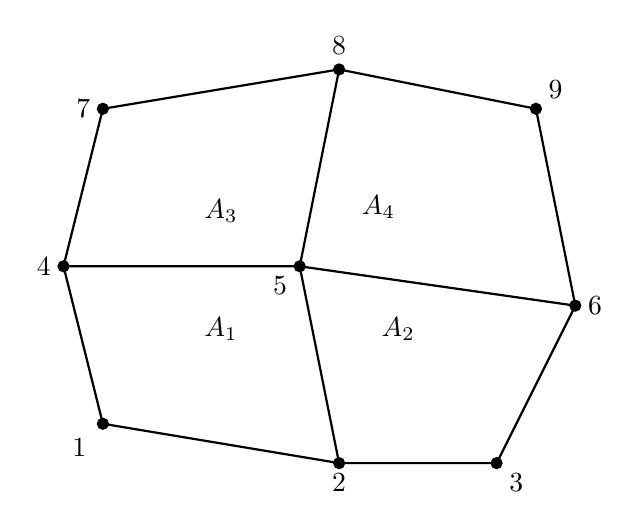
\begin{tikzpicture}
%\draw[fill=gray!5,gray!5](0,0) rectangle (9,7);
%\draw[step=0.5cm,gray,very thin] (0,0) grid (9,7); %background grid
\draw[thick](1.5,1.5) -- (4.5,1) -- (6.5,1) -- (7.5,3) -- (7,5.5) -- (4.5,6) --(1.5,5.5) -- (1,3.5) -- cycle;  
\draw[thick](4.5,1)--(4,3.5)--(4.5,6);
\draw[thick](1,3.5)--(4,3.5)--(7.5,3);
\draw[black,fill=black] (1.5,1.5) circle (2pt); \node[] at (1.2,1.2){1}; %1
\draw[black,fill=black] (4.5,1)   circle (2pt); \node[] at (4.5,0.75){2}; %2
\draw[black,fill=black] (6.5,1)   circle (2pt); \node[] at (6.75,0.75){3}; %3
\draw[black,fill=black] (1,3.5)   circle (2pt); \node[] at (0.75,3.5){4}; %4
\draw[black,fill=black] (4,3.5)   circle (2pt); \node[] at (3.75,3.25){5}; %5
\draw[black,fill=black] (7.5,3)   circle (2pt); \node[] at (7.75,3){6}; %6
\draw[black,fill=black] (1.5,5.5) circle (2pt); \node[] at (1.25,5.5){7}; %7
\draw[black,fill=black] (4.5,6)   circle (2pt); \node[] at (4.5,6.3){8}; %8
\draw[black,fill=black] (7,5.5)   circle (2pt); \node[] at (7.25,5.75){9}; %9
%\draw[thin,dashed](1,3.5)--(4.5,1)--(7.5,3)--(4.5,6)--cycle;
\node[] at (3,2.7){$A_1$}; %8
\node[] at (5.25,2.7){$A_2$}; %8
\node[] at (5,4.25){$A_4$}; %8
\node[] at (3,4.2){$A_3$}; %8
\end{tikzpicture}
\end{center}
\[
q_5^{(1)} = \frac{1}{4}\sum_{e=1}^4 p_e
\] 

In the codes which rely on the $Q_1 \times P_0$ element, the (elemental) pressure
is simply defined as 
\begin{lstlisting}
p=np.zeros(nel,dtype=np.float64)  
\end{lstlisting}
while the nodal pressure is then defined as\footnote{In virtually all stones $p$
stands for the 'raw' pressure and $q$ stands for its projection onto the velocity mesh.} 
\begin{lstlisting}
q=np.zeros(nnp,dtype=np.float64)  
\end{lstlisting}
The element-to-node algorithm is then simply (in 2D):

\begin{lstlisting}
count=np.zeros(nnp,dtype=np.int32)  
for iel in range(0,nel):
    q[icon[0,iel]]+=p[iel]
    q[icon[1,iel]]+=p[iel]
    q[icon[2,iel]]+=p[iel]
    q[icon[3,iel]]+=p[iel]
    count[icon[0,iel]]+=1
    count[icon[1,iel]]+=1
    count[icon[2,iel]]+=1
    count[icon[3,iel]]+=1
q=q/count
\end{lstlisting}



%----------------------------------------------------------------------
\paragraph{Schemes 2,3}.

{\sl Schemes 2,3} are very similar and are presented in Sani \etal (1981) \cite{sagl81a,sagl81b}.
Scheme 2 uses the areas of the surrounding elements as weights for the arithmetic averaging
while scheme 3 uses the area of the triangles:

\begin{multicols}{2}

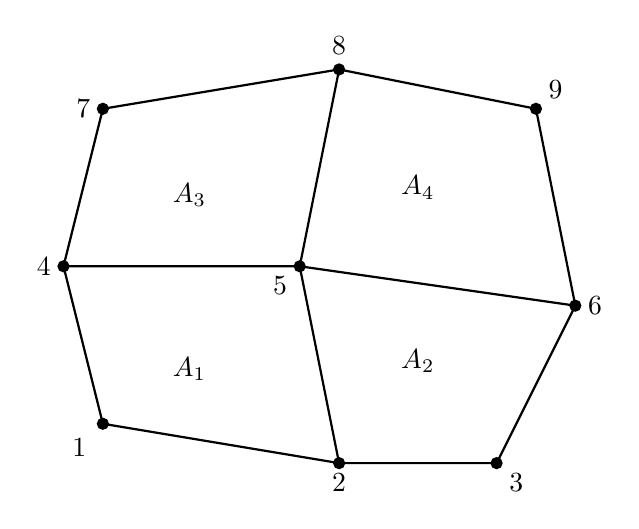
\begin{tikzpicture}
%\draw[fill=gray!5,gray!5](0,0) rectangle (9,7);
%\draw[step=0.5cm,gray,very thin] (0,0) grid (9,7); %background grid
\draw[thick](1.5,1.5) -- (4.5,1) -- (6.5,1) -- (7.5,3) -- (7,5.5) -- (4.5,6) --(1.5,5.5) -- (1,3.5) -- cycle;  
\draw[thick](4.5,1)--(4,3.5)--(4.5,6);
\draw[thick](1,3.5)--(4,3.5)--(7.5,3);
\draw[black,fill=black] (1.5,1.5) circle (2pt); \node[] at (1.2,1.2){1}; %1
\draw[black,fill=black] (4.5,1)   circle (2pt); \node[] at (4.5,0.75){2}; %2
\draw[black,fill=black] (6.5,1)   circle (2pt); \node[] at (6.75,0.75){3}; %3
\draw[black,fill=black] (1,3.5)   circle (2pt); \node[] at (0.75,3.5){4}; %4
\draw[black,fill=black] (4,3.5)   circle (2pt); \node[] at (3.75,3.25){5}; %5
\draw[black,fill=black] (7.5,3)   circle (2pt); \node[] at (7.75,3){6}; %6
\draw[black,fill=black] (1.5,5.5) circle (2pt); \node[] at (1.25,5.5){7}; %7
\draw[black,fill=black] (4.5,6)   circle (2pt); \node[] at (4.5,6.3){8}; %8
\draw[black,fill=black] (7,5.5)   circle (2pt); \node[] at (7.25,5.75){9}; %9
\node[] at (2.6,2.2){$A_1$}; %8
\node[] at (5.5,2.3){$A_2$}; %8
\node[] at (2.6,4.4){$A_3$}; %8
\node[] at (5.5,4.5){$A_4$}; %8
\end{tikzpicture}

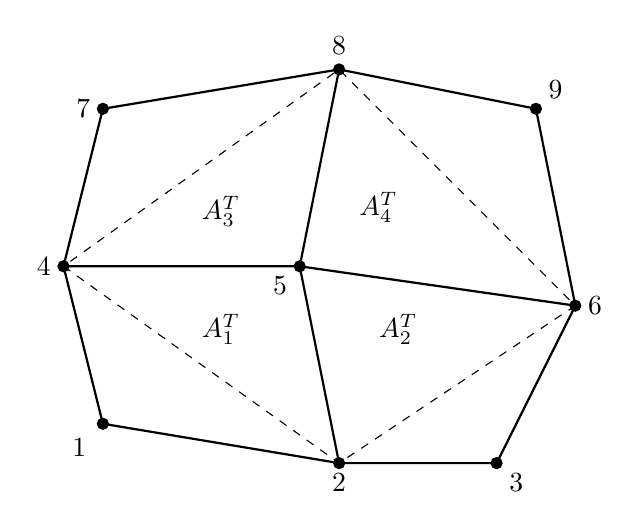
\begin{tikzpicture}
%\draw[fill=gray!5,gray!5](0,0) rectangle (9,7);
%\draw[step=0.5cm,gray,very thin] (0,0) grid (9,7); %background grid
\draw[thick](1.5,1.5) -- (4.5,1) -- (6.5,1) -- (7.5,3) -- (7,5.5) -- (4.5,6) --(1.5,5.5) -- (1,3.5) -- cycle;  
\draw[thick](4.5,1)--(4,3.5)--(4.5,6);
\draw[thick](1,3.5)--(4,3.5)--(7.5,3);
\draw[black,fill=black] (1.5,1.5) circle (2pt); \node[] at (1.2,1.2){1}; %1
\draw[black,fill=black] (4.5,1)   circle (2pt); \node[] at (4.5,0.75){2}; %2
\draw[black,fill=black] (6.5,1)   circle (2pt); \node[] at (6.75,0.75){3}; %3
\draw[black,fill=black] (1,3.5)   circle (2pt); \node[] at (0.75,3.5){4}; %4
\draw[black,fill=black] (4,3.5)   circle (2pt); \node[] at (3.75,3.25){5}; %5
\draw[black,fill=black] (7.5,3)   circle (2pt); \node[] at (7.75,3){6}; %6
\draw[black,fill=black] (1.5,5.5) circle (2pt); \node[] at (1.25,5.5){7}; %7
\draw[black,fill=black] (4.5,6)   circle (2pt); \node[] at (4.5,6.3){8}; %8
\draw[black,fill=black] (7,5.5)   circle (2pt); \node[] at (7.25,5.75){9}; %9
\draw[thin,dashed](1,3.5)--(4.5,1)--(7.5,3)--(4.5,6)--cycle;
\node[] at (3,2.7){$A_1^T$}; %8
\node[] at (5.25,2.7){$A_2^T$}; %8
\node[] at (5,4.25){$A_4^T$}; %8
\node[] at (3,4.2){$A_3^T$}; %8
\end{tikzpicture}

\end{multicols}




\[
q_5^{(2)} = \frac{\sum\limits_{e=1}^4 A_e p_e}{\sum\limits_{e=1}^4 A_e}
\qquad
\qquad
q_5^{(3)} = \frac{\sum\limits_{e=1}^4 A_e^T p_e}{\sum\limits_{e=1}^4 A_e^T}
\] 


\begin{remark} Although Schemes 1,2,3 are similar, scheme 1 is the simplest and fastest
to implement since the areas of neighbouring elements/triangles are not needed.
\end{remark}

\begin{remark} 
Schemes 1,2,3 are identical if all elements are rectangles of identical dimensions.
\end{remark}




%----------------------------------------------------------------------
\paragraph{Scheme 4} This scheme has been designed by me. 
It resembles the last three ones, but the weighing is in this case different.

Let us consider a 1D problem:
\begin{center}
\includegraphics[width=0.5\linewidth]{images/pressure_smoothing/newalgo.png}
\end{center}

Elemental pressures $p_1$ and $p_2$ corresponding to elements 1 and 2 respectively are known at
locations $x_1$ and $x_2$. The two elements have a different size, characterised in this case
by the distances $d_1$ and $d_2$ to their common edge.

The equation of the line passing through points $(x_1,p_1)$ and $(x_2,p_2)$ is 
\[
p(x)=\frac{p_2-p_1}{x_2-x_1}(x-x_1)+p_1
\]
The $x$ coordinate of the common edge is given by $x=x_1+d_1/2$, 
and since $x_2-x_1=(d_1+d_2)/2$, the 
pressure at this location writes:
\[
p(x_M)= \frac{p_2-p_1}{d_1+d_2}d_1+p_1 = \frac{\frac{p_1}{d_1} + \frac{p_2}{d_2}}{\frac{1}{d_1} + \frac{1}{d_2}}
\]
Extrapolating this formula to 2D, $d_1$ and $d_2$ are in fact the element volumes, so that
\[
q_5^{(4)} = 
\frac{\sum\limits_{j=1}^4 \frac{p_j^e}{A_j^e}}{\sum\limits_{j=1}^4 \frac{1}{A_j^e}}
=
\frac{
\frac{p_1^e}{A_1^e}+
\frac{p_2^e}{A_2^e}+
\frac{p_3^e}{A_3^e}+
\frac{p_4^e}{A_4^e}
}{
\frac{1}{A_1^e}+
\frac{1}{A_2^e}+
\frac{1}{A_3^e}+
\frac{1}{A_4^e}
}\]

There remains a problem, due to the presence of the boundary nodes for which 
the sums present in the above equation do not run up to 4. A boundary
node only has three neighbours and a corner node only two. Additional measures
are required for these nodes. 

\begin{center}
\includegraphics[width=0.5\linewidth]{images/pressure_smoothing/newalgo_corner.png}
\end{center}

The pressure value $p_N$ is obtained as follows:
\[
q_N = \frac{ 
 \frac{p_2^e}   {A_2^e}
+\frac{p_3^e}   {A_3^e}
+\frac{p_{2'}^e}{A_{2'}^e}
+\frac{p_{3'}^e}{A_{3'}^e}
}{
 \frac{1}{A_2^e}
+\frac{1}{A_3^e}
+\frac{1}{A_{2'}^e}
+\frac{1}{A_{3'}^e}
}
\]
The areas and pressures of the mirrored elements 2' and 3' are extrapolated from the areas of elements 2 and 6, and 3 and 7 respectively. 
Likewise the pressure $p_M$ at the corner node is obtained through the pressures of its surrounding elements.


%------------------------------------------------------------------------------
\paragraph{Scheme 5 - Least squares} This scheme is presented (among other places) in Lee \etal (1979)
\cite{legs79}. 
Let us start from the patch of 4 $Q_1$ elements counting 9 nodes: 

\begin{center}
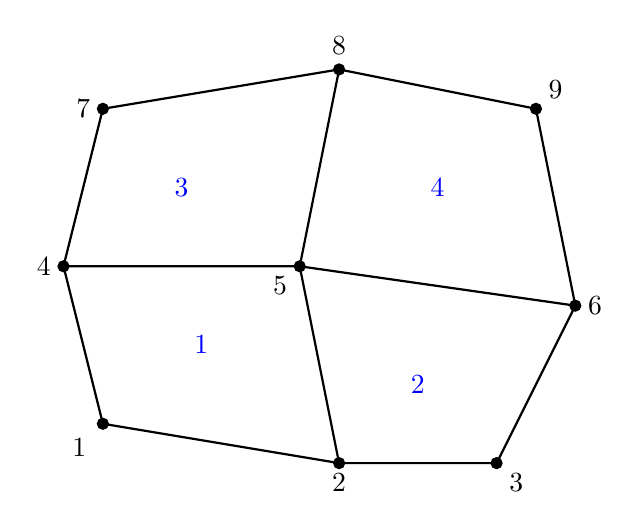
\begin{tikzpicture}
%\draw[fill=gray!5,gray!5](0,0) rectangle (9,7);
%\draw[step=0.5cm,gray,very thin] (0,0) grid (9,7); %background grid
\draw[thick](1.5,1.5) -- (4.5,1) -- (6.5,1) -- (7.5,3) -- (7,5.5) -- (4.5,6) --(1.5,5.5) -- (1,3.5) -- cycle;  
\draw[thick](4.5,1)--(4,3.5)--(4.5,6);
\draw[thick](1,3.5)--(4,3.5)--(7.5,3);

\node[] at (2.75,2.5) {\color{blue}1};
\node[] at (5.5,2) {\color{blue}2};
\node[] at (2.5,4.5) {\color{blue}3};
\node[] at (5.75,4.5) {\color{blue}4};

\draw[black,fill=black] (1.5,1.5) circle (2pt); \node[] at (1.2,1.2){1}; %1
\draw[black,fill=black] (4.5,1)   circle (2pt); \node[] at (4.5,0.75){2}; %2
\draw[black,fill=black] (6.5,1)   circle (2pt); \node[] at (6.75,0.75){3}; %3
\draw[black,fill=black] (1,3.5)   circle (2pt); \node[] at (0.75,3.5){4}; %4
\draw[black,fill=black] (4,3.5)   circle (2pt); \node[] at (3.75,3.25){5}; %5
\draw[black,fill=black] (7.5,3)   circle (2pt); \node[] at (7.75,3){6}; %6
\draw[black,fill=black] (1.5,5.5) circle (2pt); \node[] at (1.25,5.5){7}; %7
\draw[black,fill=black] (4.5,6)   circle (2pt); \node[] at (4.5,6.3){8}; %8
\draw[black,fill=black] (7,5.5)   circle (2pt); \node[] at (7.25,5.75){9}; %9

\end{tikzpicture}
\end{center}



We are looking for a field $q$ living on the nodes.
We build the quantity
\[
J=\iint_\Omega (q-p)^2 dV
\]
where $p$ is the elemental field. To make things clearer we split the integral into 
the sum of elemental integrals:
\[
J=
\iint_{\Omega_1} (q(x,y)-p_1)^2 dV+
\iint_{\Omega_2} (q(x,y)-p_2)^2 dV+
\iint_{\Omega_3} (q(x,y)-p_3)^2 dV+
\iint_{\Omega_4} (q(x,y)-p_4)^2 dV
\]
Inside each element the field $q(x,y)$ is given by a bilinear interpolation so that:
\begin{eqnarray}
J
&=& \iint_{\Omega_1} (\bN_1(x,y) q_1 + \bN_2(x,y)q_2 + \bN_5(x,y)q_5 + \bN_4(x,y)q_4 -p_1)^2 dV \nn\\
&+& \iint_{\Omega_2} (\bN_2(x,y) q_2 + \bN_3(x,y)q_3 + \bN_6(x,y)q_6 + \bN_5(x,y)q_5 -p_2)^2 dV \nn\\
&+& \iint_{\Omega_3} (\bN_4(x,y) q_4 + \bN_5(x,y)q_5 + \bN_8(x,y)q_8 + \bN_7(x,y)q_7 -p_3)^2 dV \nn\\
&+& \iint_{\Omega_4} (\bN_5(x,y) q_5 + \bN_6(x,y)q_6 + \bN_9(x,y)q_9 + \bN_8(x,y)q_8 -p_4)^2 dV 
\end{eqnarray}
where the $N_i$ functions are the basis functions (unusually expressed in $x,y$ coordinates).
The least square procedure looks for the set of $q_i$ such that 
\[
\frac{\partial J}{\partial q_i} =0 \qquad \forall i=1,...9
\]
and this yields 9 equations/constraints for 9 unknowns.
\begin{eqnarray}
\frac{\partial J}{\partial q_1} 
&=& \iint_{\Omega_1} 2 (\bN_1(x,y) q_1 + \bN_2(x,y)q_2 + \bN_5(x,y)q_5 + \bN_4(x,y)q_4 -p_1) \bN_1(x,y) dV \nn\\
\frac{\partial J}{\partial q_2}
&=& \iint_{\Omega_1} 2(\bN_1(x,y) q_1 + \bN_2(x,y)q_2 + \bN_5(x,y)q_5 + \bN_4(x,y)q_4 -p_1) \bN_2(x,y) dV \nn\\
&+& \iint_{\Omega_2} 2(\bN_2(x,y) q_2 + \bN_3(x,y)q_3 + \bN_6(x,y)q_6 + \bN_5(x,y)q_5 -p_2) \bN_2(x,y) dV \nn\\
\frac{\partial J}{\partial q_3}
&=& \iint_{\Omega_2} 2(\bN_2(x,y) q_2 + \bN_3(x,y)q_3 + \bN_6(x,y)q_6 + \bN_5(x,y)q_5 -p_2) \bN_3(x,y) dV \nn\\
\frac{\partial J}{\partial q_4}
&=& \iint_{\Omega_1} 2(\bN_1(x,y) q_1 + \bN_2(x,y)q_2 + \bN_5(x,y)q_5 + \bN_4(x,y)q_4 -p_1) \bN_4(x,y) dV \nn\\
&+& \iint_{\Omega_3} 2(\bN_4(x,y) q_4 + \bN_5(x,y)q_5 + \bN_8(x,y)q_8 + \bN_7(x,y)q_7 -p_3) \bN_4(x,y) dV \nn\\
\frac{\partial J}{\partial q_5}
&=& \iint_{\Omega_1} 2(\bN_1(x,y) q_1 + \bN_2(x,y)q_2 + \bN_5(x,y)q_5 + \bN_4(x,y)q_4 -p_1) \bN_5(x,y) dV \nn\\
&+& \iint_{\Omega_2} 2(\bN_2(x,y) q_2 + \bN_3(x,y)q_3 + \bN_6(x,y)q_6 + \bN_5(x,y)q_5 -p_2) \bN_5(x,y) dV \nn\\
&+& \iint_{\Omega_3} 2(\bN_4(x,y) q_4 + \bN_5(x,y)q_5 + \bN_8(x,y)q_8 + \bN_7(x,y)q_7 -p_3) \bN_5(x,y) dV \nn\\
&+& \iint_{\Omega_4} 2(\bN_5(x,y) q_5 + \bN_6(x,y)q_6 + \bN_9(x,y)q_9 + \bN_8(x,y)q_8 -p_4) \bN_5(x,y) dV \nn\\
\frac{\partial J}{\partial q_6}
&=& \iint_{\Omega_2} 2(\bN_2(x,y) q_2 + \bN_3(x,y)q_3 + \bN_6(x,y)q_6 + \bN_5(x,y)q_5 -p_2) \bN_6(x,y) dV \nn\\
&+& \iint_{\Omega_4} 2(\bN_5(x,y) q_5 + \bN_6(x,y)q_6 + \bN_9(x,y)q_9 + \bN_8(x,y)q_8 -p_4) \bN_6(x,y) dV \nn\\
\frac{\partial J}{\partial q_7}
&=& \iint_{\Omega_3} 2(\bN_4(x,y) q_4 + \bN_5(x,y)q_5 + \bN_8(x,y)q_8 + \bN_7(x,y)q_7 -p_3) \bN_7(x,y) dV \nn\\
\frac{\partial J}{\partial q_8}
&=& \iint_{\Omega_3} 2(\bN_4(x,y) q_4 + \bN_5(x,y)q_5 + \bN_8(x,y)q_8 + \bN_7(x,y)q_7 -p_3) \bN_8(x,y)dV \nn\\
&+& \iint_{\Omega_4} 2(\bN_5(x,y) q_5 + \bN_6(x,y)q_6 + \bN_9(x,y)q_9 + \bN_8(x,y)q_8 -p_4) \bN_8(x,y)dV \nn\\ 
\frac{\partial J}{\partial q_9}
&=& \iint_{\Omega_4} 2(\bN_5(x,y) q_5 + \bN_6(x,y)q_6 + \bN_9(x,y)q_9 + \bN_8(x,y)q_8 -p_4) \bN_9(x,y)dV 
\end{eqnarray}
The factor 2 are removed and the terms $\int p_i N_j $ are known so they end up in the right hand side.
\begin{eqnarray}
 \iint_{\Omega_1} (\bN_1 \bN_1 q_1 + \bN_1 \bN_2 q_2 + \bN_1 \bN_5 q_5 + \bN_1 \bN_4 q_4) dV 
&=& \iint_{\Omega_1} p_1 N_1 dV \nn\\
 \iint_{\Omega_1} (\bN_2 \bN_1 q_1 + \bN_2 \bN_2 q_2 + \bN_2 \bN_5 q_5 + \bN_2 \bN_4 q_4) dV \nn\\
+\iint_{\Omega_2} (\bN_2 \bN_2 q_2 + \bN_3 \bN_2 q_3 + \bN_6 \bN_2 q_6 + \bN_5 \bN_2 q_5) dV 
&=& \iint_{\Omega_1} p_1N_2 dV + \iint_{\Omega_2}  p_2 \bN_2 dV \nn\\
\nn\\
\dots &=& \dots \nn\\
\nn\\
 \iint_{\Omega_4} (\bN_9\bN_5 q_5 + \bN_9\bN_6q_6 + \bN_9\bN_9q_9 + \bN_9\bN_8q_8) dV &=&  \iint_{\Omega_4} p_4 \bN_9 dV 
\end{eqnarray}

The mass matrices corresponding to the four elements are 
\[
{\bm M}_1 = \int_{\Omega_1} \left( \begin{array}{cccc}
 \bN_1 \bN_1 & \bN_1 \bN_2 & \bN_1 \bN_5 & \bN_1 \bN_4 \\
 \bN_2 \bN_1 & \bN_2 \bN_2 & \bN_2 \bN_5 & \bN_2 \bN_4 \\
 \bN_5 \bN_1 & \bN_5 \bN_2 & \bN_5 \bN_5 & \bN_5 \bN_4 \\
 \bN_4 \bN_1 & \bN_4 \bN_2 & \bN_4 \bN_5 & \bN_4 \bN_4 
\end{array}\right) dV
\qquad
{\bm M}_2 = \int_{\Omega_2} \left( \begin{array}{cccc}
 \bN_2 \bN_2 & \bN_2 \bN_3 & \bN_2 \bN_6 & \bN_2 \bN_5 \\
 \bN_3 \bN_2 & \bN_3 \bN_3 & \bN_3 \bN_6 & \bN_3 \bN_5 \\
 \bN_6 \bN_2 & \bN_6 \bN_3 & \bN_6 \bN_6 & \bN_6 \bN_5 \\
 \bN_5 \bN_2 & \bN_5 \bN_3 & \bN_5 \bN_6 & \bN_5 \bN_5 
\end{array}\right) dV
\]
\[
{\bm M}_3 = \int_{\Omega_3} \left( \begin{array}{cccc}
 \bN_4 \bN_4 & \bN_4 \bN_5 & \bN_4 \bN_8 & \bN_4 \bN_7 \\
 \bN_5 \bN_4 & \bN_5 \bN_5 & \bN_5 \bN_8 & \bN_5 \bN_7 \\
 \bN_8 \bN_4 & \bN_8 \bN_5 & \bN_8 \bN_8 & \bN_8 \bN_7 \\
 \bN_7 \bN_4 & \bN_7 \bN_5 & \bN_7 \bN_8 & \bN_7 \bN_7 
\end{array}\right) dV
\qquad
{\bm M}_4 = \int_{\Omega_4} \left( \begin{array}{cccc}
 \bN_5 \bN_5 & \bN_5 \bN_6 & \bN_5 \bN_9 & \bN_5 \bN_8 \\
 \bN_6 \bN_5 & \bN_6 \bN_6 & \bN_6 \bN_9 & \bN_6 \bN_8 \\
 \bN_9 \bN_5 & \bN_9 \bN_6 & \bN_9 \bN_9 & \bN_9 \bN_8 \\
 \bN_8 \bN_5 & \bN_8 \bN_6 & \bN_8 \bN_9 & \bN_8 \bN_8 
\end{array}\right) dV
\]
so that the 9 equations above are actually the result of the assembly process of these four 
elemental systems:
\[
\left( \iint_{\Omega_e} \vec{\bN}^T\vec{\bN} dV \right) \cdot \vec{q}_e = \iint_{\Omega_i} \vec{\bN}^T p_e dV 
\qquad\qquad e=1,2,3,4
\]


%------------------------------------------------------------------------------
\paragraph{Scheme 6 - Consistent pressure recovery}

The is the method presented in Zienkiewicz \& Nakazawa (1982) \cite{zina82}. In the second part 
of this publication the authors wish to establish a simple and effective numerical method to calculate 
variables eliminated by the penalisation process. 
The method involves an additional finite element solution for the nodal pressures using 
the same finite element basis and numerical quadrature as used for the velocity.

Let us start with\footnote{I here voluntarily use $q$ instead of $p$}:
\[
q = -\lambda \vec\nabla\cdot \vec\upnu
\]
We are going to treat this equation as any other PDE in the context of the FE method, i.e. 
we are going to establish its weak form. 
We assume that the pressure is given inside an element by
\[
q(x,y) = \sum_{i=1}^4 \bN_i(x,y) q_i = \vec{\bN} \cdot \vec{q}
\]
and the velocity:
\[
\vec\upnu = (u,v) 
\qquad 
\qquad 
u(x,y)  = \sum_{i=1}^4 \bN_i(x,y) u_i
\qquad 
\qquad 
v(x,y)  = \sum_{i=1}^4 \bN_i(x,y) v_i
\]
where the $\bN_i$ are the $Q_1$ basis functions and $q_i$ are the sought after nodal values. 
We multiply the equation above by a $Q_1$ basis function $\bN_i$ and integrate over the whole domain:
\[
\iint_\Omega \bN_i(x,y) q(x,y) \; dxdy 
= -\lambda \iint_\Omega \bN_i \vec\nabla\cdot \vec\upnu  \; dx dy
\]
As before we now focus on the above expression inside a single element $e$:
\[
\iint_{\Omega_e} \bN_i(x,y) q(x,y) \; dxdy = -\lambda \iint_{\Omega_e} \bN_i \vec\nabla\cdot \vec\upnu \; dx dy
\]
After $\bN_i \rightarrow \vec{\bN}=(\bN_1,\bN_2,\bN_3,\bN_4)^T$, the left hand side term becomes:
\[
\iint _{\Omega_e} \vec{\bN}^T q(x,y) \; dxdy 
=
\iint _{\Omega_e} \vec{\bN}^T \vec{\bN} \cdot \vec{q} \; dxdy 
=
\left(\underbrace{\iint _{\Omega_e} \vec{\bN}^T \vec{\bN} dxdy}_{{\bm M}_e} \right) \cdot \vec{q}  
\]
where ${\bm M}_e$ is the elemental mass matrix.
We now turn to the right hand side. We have
\[
\vec\nabla\cdot \vec\upnu
= \frac{\partial u}{\partial x}+\frac{\partial v}{\partial y}
= \sum_i \frac{\partial \bN_i}{\partial x} u_i + \sum_i \frac{\partial \bN_i}{\partial y} v_i 
\]
We here too define $\vec{V}_e=(u_1,v_1,u_2,v_2,u_3,v_3,u_4,v_4)^T$ so that 

\begin{eqnarray}
&& \iint_{\Omega_e} \vec{\bN} {\vec \nabla}\cdot {\vec \upnu} \; dV \nn\\
&=& \iint_{\Omega_e} \vec{\bN}^T \sum_{i=1}^{4} 
\left( \frac{\partial \bN_i}{\partial x} u_i + \frac{\partial \bN_i}{\partial y} v_i 
\right)  
dV \nonumber\\
&=& 
\iint_{\Omega_e} 
\left(
\begin{array}{c}
\bN_1 \left(
\sum\limits_{i=1}^{4} \frac{\partial \bN_i}{\partial x} u_i +
\sum\limits_{i=1}^{4} \frac{\partial \bN_i}{\partial y} v_i \right) \\
\bN_2 \left(
\sum\limits_{i=1}^{4} \frac{\partial \bN_i}{\partial x} u_i +
\sum\limits_{i=1}^{4} \frac{\partial \bN_i}{\partial y} v_i \right) \\
\bN_3 \left(
\sum\limits_{i=1}^{4} \frac{\partial \bN_i}{\partial x} u_i +
\sum\limits_{i=1}^{4} \frac{\partial \bN_i}{\partial y} v_i \right) \\
\bN_4 \left(
\sum\limits_{i=1}^{4} \frac{\partial \bN_i}{\partial x} u_i +
\sum\limits_{i=1}^{4} \frac{\partial \bN_i}{\partial y} v_i \right) 
\end{array}
\right) dV \nonumber \\  %%%%%%%%%%%%%%%%%%%%%%%%%%
&=& 
\int_{\Omega_e} 
\left(
\begin{array}{ccc}
{\bN}_1& {\bN}_1 &  0 \\\\
{\bN}_2& {\bN}_2 &  0 \\\\
{\bN}_3& {\bN}_3 &  0 \\\\
{\bN}_4& {\bN}_4 &  0 
\end{array}
\right)
\cdot
\left(
\begin{array}{c}
\sum\limits_i \frac{\partial \bN_i}{\partial x} u_i \\ \\
\sum\limits_i \frac{\partial \bN_i}{\partial y} v_i \\ \\
\sum\limits_i (\frac{\partial \bN_i}{\partial y} u_i\! +\! \frac{\partial \bN_i}{\partial x} v_i) 
\end{array}
\right)
\; dV \nonumber\\ %%%%%%%%%%%%%%%%%%%%%%%%%%
&=& 
\int_{\Omega_e} 
\underbrace{
\left(
\begin{array}{cccccc}
{\bN}_1 & {\bN}_1 &  0 \\
{\bN}_2 & {\bN}_2 &  0 \\
{\bN}_3 & {\bN}_3 &  0 \\
{\bN}_4 & {\bN}_4 &  0 
\end{array}
\right)
}_{{\bm N}}
\cdot
\underbrace{
\left(\begin{array}{cccccccc}
\partial_x \bN_1 & 0 &  
\partial_x \bN_2 & 0 &  
\partial_x \bN_3 & 0 &  
\partial_x \bN_4 & 0 \\ \\
0 & \partial_y \bN_1 &   
0 & \partial_y \bN_2 &   
0 & \partial_y \bN_3 &   
0 & \partial_y \bN_4 \\ \\
\partial_y \bN_1 & \partial_x \bN_1 &  
\partial_y \bN_2 & \partial_x \bN_2 &  
\partial_y \bN_3 & \partial_x \bN_3 &  
\partial_y \bN_4 & \partial_x \bN_4 
\end{array}\right)}_{{\bm B}}
\cdot \vec{V}_e
\; dV  \nonumber \\
&=& 
\left(\int_{\Omega_e} {\bm N} \cdot {\bm B} \; dV \right) \cdot \vec{V}_e \nonumber\\
&=& -\G_e^T \cdot {\vec V}_e
\end{eqnarray}

After assembly we arrive at
\[
{\bm M} \cdot \vec{q} = \lambda \G^T \cdot {\vec V} 
\qquad
\text{with}
\qquad
\G_e = -\int_{\Omega_e} {\bm N} \cdot {\bm B} \; dV
\]
where ${\bm M}$ is the global mass matrix, $\vec{q}$ the vector of all 
nodal pressures, $\G$ the discrete gradient matrix and $\vec{V}$
the (velocity) solution vector. 
The system can be easily solved since the mass matrix is a friendly matrix.
The vector ${\vec q}$ contains the nodal pressure values directly, with 
no need for a smoothing scheme! 

\begin{remark}
Very importantly, the mass matrix ${\bm M}$ is to be evaluated at the full integration points, 
while the constraint part (the right hand side of the equation) is to be evaluated at 
the reduced integration point, i.e. in the middle of the element.  
\end{remark}

\begin{remark}
As noted in \cite{zina82}, it is interesting to note that when linear elements are used 
and the lumped matrices are used for the ${\bm M}$ the resulting algebraic equation is identical 
to the smoothing scheme 1 only if a uniform square finite element 
mesh is used. In this respect this method is expected to yield different results when elements 
are not square or even rectangular.
\end{remark}

\begin{remark}
The third column of the matrix ${\bm N}$
and the last line of the ${\bm B}$ matrix could be removed altogether.
If your code is based on the mixed formulation, then you already 
have built matrix $\G$ so you can easily re-use this piece of code 
to compute $\G$ again, this time with a reduced integration quadrature.
If you are using the penalty formulation then you need to program 
all from scratch and then simply do away with these unnecessary terms, or 
you can direcly build the rhs as $\int_{\Omega_e} \vec{\bN}^T p_e$ (assuming
you have previously computed the pressure in the middle of each element 
by means of $p=-\lambda\vec\nabla\cdot\vec\upnu$).
\end{remark}

\begin{remark}
This  scheme is identical to the least square scheme!
\end{remark}


%--------------------------------------------------------------
\paragraph{Scheme 7}

Same as scheme 6, but with lumped mass matrix.  


%--------------------------------------------------------------
\paragraph{Scheme 8 - bilinear interpolation} Let us assume that the centers of the 
four elements make a $Q_1$ quadrilateral element, as shown on this figure:


\begin{center}
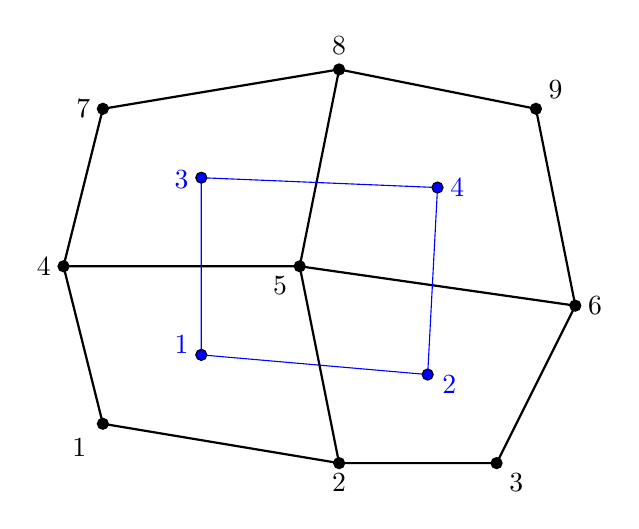
\begin{tikzpicture}
%\draw[fill=gray!5,gray!5](0,0) rectangle (9,7);
%\draw[step=0.5cm,gray,very thin] (0,0) grid (9,7); %background grid
\draw[thick](1.5,1.5) -- (4.5,1) -- (6.5,1) -- (7.5,3) -- (7,5.5) -- (4.5,6) --(1.5,5.5) -- (1,3.5) -- cycle;  
\draw[thick](4.5,1)--(4,3.5)--(4.5,6);
\draw[thick](1,3.5)--(4,3.5)--(7.5,3);

\draw[black,fill=blue] (2.75,2.375) circle (2pt); 
\node[] at (2.5,2.5) {\color{blue}1};
\draw[black,fill=blue] (5.625,2.125) circle (2pt); 
\node[] at (5.9,2) {\color{blue}2};
\draw[black,fill=blue] (5.75,4.5) circle (2pt); 
\node[] at (2.5,4.6) {\color{blue}3};
\draw[black,fill=blue] (2.75,4.625) circle (2pt); 
\node[] at (6,4.5) {\color{blue}4};

\draw[black,fill=black] (1.5,1.5) circle (2pt); \node[] at (1.2,1.2){1}; %1
\draw[black,fill=black] (4.5,1)   circle (2pt); \node[] at (4.5,0.75){2}; %2
\draw[black,fill=black] (6.5,1)   circle (2pt); \node[] at (6.75,0.75){3}; %3
\draw[black,fill=black] (1,3.5)   circle (2pt); \node[] at (0.75,3.5){4}; %4
\draw[black,fill=black] (4,3.5)   circle (2pt); \node[] at (3.75,3.25){5}; %5
\draw[black,fill=black] (7.5,3)   circle (2pt); \node[] at (7.75,3){6}; %6
\draw[black,fill=black] (1.5,5.5) circle (2pt); \node[] at (1.25,5.5){7}; %7
\draw[black,fill=black] (4.5,6)   circle (2pt); \node[] at (4.5,6.3){8}; %8
\draw[black,fill=black] (7,5.5)   circle (2pt); \node[] at (7.25,5.75){9}; %9

\draw[blue](2.75,2.375)--(5.625,2.125)--(5.75,4.5)--(2.75,4.625)--cycle;
\end{tikzpicture}
\end{center}




The values at the corners are $p_1$,
$p_2$, $p_3$ and $p_4$. Assuming that the pressure inside this element can be represented 
by a bilinear field, we have 
\[
p(x,y)= a+ bx +cy +dxy
\]
where the coefficients will be determined by ensuring that $p(x_i,y_i)=p_i$ for $i=1,2,3,4$, or:
\begin{eqnarray}
a+bx_1+cy_1+dx_1y_1 &=& p_1 \\
a+bx_2+cy_2+dx_2y_2 &=& p_2 \\
a+bx_3+cy_3+dx_3y_3 &=& p_3 \\
a+bx_4+cy_4+dx_4y_4 &=& p_4 
\end{eqnarray}
i.e.
\[
\left(
\begin{array}{cccc}
1 & x_1 & y_1 & x_1y_1 \\
1 & x_2 & y_2 & x_2y_2 \\
1 & x_3 & y_3 & x_3y_3 \\
1 & x_4 & y_4 & x_4y_4
\end{array}
\right)\cdot
\left(
\begin{array}{c}
a \\b\\c\\d
\end{array}
\right)
=
\left(
\begin{array}{c}
p_1\\p_2\\p_3\\p_4
\end{array}
\right)
\]

There remains an issue with nodes which are on the boundaries of the domain. These are of course not 
'surrounded' by four pressure values so the above algorithm does not apply directly. However, looking 
at the above figure, and assuming that node 1 is a lower left corner of a 2D domain, we can use the 
bilinear interpolation based on elements 1,2,3,4 to extrapolate a nodal pressure value at node 1. 
The same would apply for nodes 2 and 4 for example. 

\begin{remark}
This scheme is not applicable to quadtree-based meshed.
\end{remark}




 %-------------------
\newpage %---------------------------------------------------------------------
\subsection{Pressure scaling} \index{general}{pressure scaling}
\begin{flushright} {\tiny {\color{gray} pressure\_scaling.tex}} \end{flushright}
%~~~~~~~~~~~~~~~~~~~~~~~~~~~~~~~~~~~~~~~~~~~~~~~~~~~~~~~~~~~~~~~~~~~~~~~~~~~~~~~~~~~~~~~~~~~~~~~~~~

As nicely explained in the 
step 32 of deal.ii\footnote{\url{https://www.dealii.org/9.0.0/doxygen/deal.II/step\_32.html}},
we often need to scale the $\G$ block since it is many orders of magnitude smaller than $\K$ (especially in geodynamics where viscosities are $\sim 10^{22}$), 
which introduces large inaccuracies in the solving process to the point that the solution is nonsensical. 
This scaling coefficient is $\eta/L$ where $\eta$ and $L$ are representative viscosities and lengths. 
We start from 
\[
\left(
\begin{array}{cc}
\K & \G \\ \G^T & -\C 
\end{array}
\right)
\cdot
\left(
\begin{array}{c}
\vec{\cal V} \\ \vec{\cal P}
\end{array}
\right)
=
\left(
\begin{array}{c}
\vec{f} \\ \vec{h}
\end{array}
\right)
\]
and introduce the scaling coefficient as follows (which in fact does not alter the solution at all):
\[
\left(
\begin{array}{cc}
\K & \frac{\eta}{L}\G \\ \frac{\eta}{L}\G^T & - \frac{\eta^2}{L^2} \C 
\end{array}
\right)
\cdot
\left(
\begin{array}{c}
\vec{\cal V} \\\frac{L}{\eta} \vec{\cal P}
\end{array}
\right)
=
\left(
\begin{array}{c}
 \vec{f} \\ \frac{\eta}{L} \vec{h}
\end{array}
\right)
\]
We then end up with the modified Stokes system:
\[
\left(
\begin{array}{cc}
\K & \underline{\G} \\ \underline{\G}^T & \underline{\C} 
\end{array}
\right)
\cdot
\left(
\begin{array}{c}
\vec{\cal V} \\ \underline{\vec{\cal P}}
\end{array}
\right)
=
\left(
\begin{array}{c}
\vec{f} \\ \underline{\vec{h}}
\end{array}
\right)
\]
where 
\[
\underline{\G}=\frac{\eta}{L}\G
\quad\quad
\quad\quad
\underline{\vec{\cal P}}=\frac{L}{\eta} \vec{\cal P}
\quad\quad
\quad\quad
\underline{\C}=\frac{\eta^2}{L^2} \C
\quad\quad
\quad\quad
\underline{\vec{h}}=\frac{\eta}{L}\vec{h}
\]
After the solve phase, we recover the real pressure with $\vec{\cal P}=\frac{\eta}{L}\underline{\vec{\cal P}}$.

Note that in Section~\ref{sec:block_scaling} we revisit the topic and this time 
scale all the blocks of the Stokes matrix.



 %-----------------------
\newpage %---------------------------------------------------------------------
\subsection{Pressure normalisation\label{ss_pnorm}} 
%..................................................
\subsubsection{Basic idea and naive implementation}

When Dirichlet boundary conditions are imposed everywhere on the boundary, pressure is only present by its gradient in 
the equations. It is thus determined up to an arbitrary constant (one speaks then of a null space of size 1).  
In such a case, one commonly impose the average of the pressure over the whole domain or on a subsect of the boundary 
to be have a zero average, i.e.
\[
\int_\Omega p dV = 0
\]
Another possibility is to impose the pressure value at a single node. 

Let us assume that we are using $Q_1 \times P_0$ elements. Then the pressure is constant 
inside each element. 
The integral above becomes:
\[
\int_\Omega p dV = 
\sum_e  \int_{\Omega_e} p dV = 
\sum_e  p_e \int_{\Omega_e} dV = 
\sum_e  p_e A_e = 0
\]
where the sum runs over all elements $e$ of area $A_e$.
This can be rewritten 
\[
\LLL^T \cdot \vec{\cal P}=0
\] 
and it is a constraint on the pressure solution. 
As we have seen before \ref{XXX}, we can associate to it a 
Lagrange multiplier $\lambda$ so that we must solve the modified Stokes system:
\[
\left(
\begin{array}{ccc}
\K & \G & 0\\ 
\G^T & 0 & \LLL \\
0 & \LLL^T & 0
\end{array}
\right)
\cdot
\left(
\begin{array}{c}
\vec{\cal V} \\ \vec{\cal P} \\ \lambda
\end{array}
\right)
=
\left(
\begin{array}{c}
\vec{f} \\ \vec{h} \\ 0
\end{array}
\right)
\]
When higher order spaces are used for pressure (continuous or discontinuous)
one must then carry out the above integration numerically by means of (usually)
a Gauss-Legendre quadrature.

Although valid, this approach has one main disadvantage: it makes the Stokes matrix larger (although
marginally so -- only one row and column are added), but more importantly it prevents the use of some
of the solving strategies of Section \ref{solvers}.


%..................................................
\subsubsection{Implementation -- the real deal}

The idea is actually quite simple and requires two steps:
\begin{enumerate}
\item remove the null space by prescribing the pressure at one location and solve the system;
\item post-process the pressure so as to arrive at a pressure field which fulfills the required normalisation (surface, volume, ...)
\end{enumerate}

\todo[inline]{finish explain}






 %--
\newpage %----------------------------------------------------------------------------
\subsection{Solving the Stokes system \label{sec:solvers}} \begin{flushright} {\tiny {\color{gray} \tt solvers.tex}} \end{flushright}
%~~~~~~~~~~~~~~~~~~~~~~~~~~~~~~~~~~~~~~~~~~~~~~~~~~~~~~~~~~~~~~~~~~~~~~~~~~~~~~~~~~~~~~~~~~~~~~~~~~

Let us start again from the (full) Stokes system:
\begin{equation}
\underbrace{
\left(
\begin{array}{cc}
\K & \G \\ \G^T & -\C 
\end{array}
\right)
}_{\cal A}
\cdot
\left(
\begin{array}{c}
\vec{\cal V} \\ \vec{\cal P}
\end{array}
\right)
=
\left(
\begin{array}{c}
\vec{f} \\ \vec{h}
\end{array}
\right)
\label{StokesSyst}
\end{equation}
We need to solve this system in order to obtain the solution, i.e. the $\vec{\cal V}$ 
and $\vec{\cal P}$ vectors. But how? 
Unfortunately, this question is not simple to answer and the appropriate method depends on many 
parameters, but mainly on how big the matrix blocks are and what the condition number of the matrix $\K$ is. 

First let us start with an obvious question: couldn't we just compute the inverse of the matrix ${\cal A}$?
Under the assumption that the inverse of $\K$ and $\SSS$ exists, we can and we find\footnote{The matrix 
$\C$ is here omitted but it bears no consequences on the conclusion.}
\[
{\cal A}^{-1} = 
\left(
\begin{array}{cc}
\K & \G \\ \G^T & 0
\end{array}
\right)^{-1}
=
\left(
\begin{array}{cc}
\K^{-1} + \K^{-1} \cdot \G \cdot\SSS^{-1} \cdot\G^T \cdot\K^{-1} & -\K^{-1} \cdot\G \cdot\SSS^{-1} \\ 
-\SSS^{-1} \cdot\G^T \cdot\K^{-1}  &  \SSS^{-1}
\end{array}
\right)
\]
However, such an expression is of limited interest in the numerical solution of saddle
point problems since it showcases 5 times the inverse of $\K$ and more importantly
the inverse of the Schur complement matrix $\SSS$ which is likely to be a full matrix so 
that we never want to compute it explicitely.


As concisely explained in Clevenger \& Heister (2021) \cite{clhe21}, 
there are three common approaches used in the literature for solving the above equation on large scales:
\begin{itemize}
\item a pressure corrected, Schur complement CG scheme, using multigrid as an 
approximation to the velocity block;
\item a block-preconditioned Krylov
method, also using multigrid on the velocity block.
For this method, there are two main types:
\begin{itemize}
\item GMRES\cite{mabl15,rumi15} (or any Krylov method not requiring symmetry) with
block-triangular preconditioner (This is what \aspect does):
\[
{\bm P} = \left(
\begin{array}{cc}
\K & \G \\
0 & - \SSS
\end{array}
\right)
\]

\item MINRES\cite{gmhj16} with block-diagonal preconditioner
\[
{\bm P} = \left(
\begin{array}{cc}
\K & 0 \\
0 & - \SSS
\end{array}
\right)
\]

\end{itemize}

\item an all-at-once multigrid performed on the entire Stokes system, using Uzawa-type smoothers.
\end{itemize}



\Literature: Preconditioners for Incompressible Navier-Stokes Solvers 
\begin{small}
\begin{itemize}
\item \fullcite{benz02}
\item \fullcite{bewa08}
\item \fullcite{urvs08}
\item \fullcite{seuv10}
\item Saddle point preconditioners have been extensively discussed and studied \cite{bewa08}, \cite{dewu04}
\item Diagonal preconditioners in \cite{shrb01}, \cite{babc94}.
\end{itemize}
\end{small}

\Literature: Solving Stokes Saddle Point problem
\begin{small}
\begin{itemize}
\item \fullcite{laqu86}
\item \fullcite{rotf90}
\item \fullcite{frha93}
\item \fullcite{elgo94}
\item \fullcite{cheb96}, \fullcite{elma96}
\item \fullcite{brpv97}
\item \fullcite{lixu01}
\item \fullcite{dogs06}, \fullcite{lica06}
\item \fullcite{hoow17}
\item Pragmatic solvers for 3D Stokes problems with heterogeneous coefficients \cite{samb20}
\end{itemize}
\end{small}



%------------------------------------------------------------------------------
\subsection{Block diagonal scaling} \label{sec:block_scaling}

We have already seen in Section~\ref{pscaling} how and why we scale the $\G$ block. 
We revisit this topic more thoroughly in what follows.
This section is borrowed from Section~2.6 of \textcite{mamo08} (2008).

Let us state again the equation we wish to solve (Eq. 6 in the paper):
\[
\begin{pmatrix}
\K & \G \\
\G^T & 0
\end{pmatrix}
\cdot
\begin{pmatrix}
\vec{\cal V} \\
\vec{\cal P}
\end{pmatrix}
=
\begin{pmatrix}
\vec{f} \\
\vec{h}
\end{pmatrix}
\]

Prior to solving this equation, the autors apply a row/column scaling to the equation
to effectively normalize the operators $\K$ and $\G$ with the intention of
reducing round off errors. The scaling is particularly important for
problems in geodynamics when dimensional quantities are used to
define the problem and because of the large, local variations which
may occur in the constitutive tensor (in practice, the effective viscosity) . 

They apply a symmetric block diagonal scaling to the equation via the scaling matrix\footnote{
The $S$ stands for 'scaling', the Schur complement is given by $\SSS$}
\[
{\bm S} = 
\begin{pmatrix}
{\bm S}_1 & 0 \\ 0 & {\bm S}_2
\end{pmatrix}
\]
Writing the first equation as ${\bm A} \cdot \vec{x} = \vec{b}$, 
the symmetric scaling operation is applied as follows:
\[
{\bm S}^{-1} \cdot {\bm A} \cdot \vec{x}= {\bm S}^{-1} \cdot \vec{b} 
\]
followed by\footnote{${\bm S}^{-T}$ is the inverse of the transpose of the matrix.} 
\[
{\bm S}^{-1} \cdot {\bm A} \cdot {\bm S}^{-T} \cdot {\bm S}^T \cdot \vec{x}= {\bm S}^{-1} \cdot \vec{b} 
\]
to give the scaled system ${\bm A}_s \cdot \vec{y}_s = \vec{b}_s$ , where the operator 
${\bm A}_s$ is given by
\begin{eqnarray}
{\bm S}^{-1} \cdot {\bm A} \cdot {\bm S}^{-T} 
&=&\begin{pmatrix}
{\bm S}_1^{-1} & 0 \\ 0 & {\bm S}_2^{-1}
\end{pmatrix}
\cdot 
\begin{pmatrix}
\K & \G \\
\G^T & 0
\end{pmatrix}
\cdot
\begin{pmatrix}
{\bm S}_1^{-T} & 0 \\ 0 & {\bm S}_2^{-T}
\end{pmatrix} \nn\\
&=&
\begin{pmatrix}
{\bm S}_1^{-1} \cdot \K \cdot {\bm S}_1^{-T} & {\bm S}_1^{-1} \cdot \G \cdot {\bm S}_2^{-T} \\
({\bm S}_1^{-1} \cdot \G \cdot {\bm S}_2^{-T})^{T} & 0 
\end{pmatrix} \nn\\
&=&
\begin{pmatrix}
\K_s & \G_s \\
\G^T_s & 0
\end{pmatrix} \nn\\
&=&{\bm A}_s \nn
\end{eqnarray}
with
\[
{\bm S}^T \cdot \vec{x} 
= 
\begin{pmatrix}
{\bm S}_1^T \cdot \vec{\cal V} \\
{\bm S}_2^T \cdot \vec{\cal P}
\end{pmatrix}
=\vec{y}_s
\qquad\qquad
{\bm S}^{-1} \cdot \vec{b} = 
\begin{pmatrix}
{\bm S}_1^{-1}\cdot\vec{f} \\
{\bm S}_2^{-1}\cdot\vec{h}
\end{pmatrix}
=\vec{b}_s
\]
Following the solution of the scaled system, we recover the un-scaled
solution from $\vec{x} = {\bm S}^{-T} \cdot  \vec{y}_s$. 
The form of the scaling operation is based
on the preconditioner described in Rusten and Winther (1992). For
the purpose of scaling, rather than full preconditioning of the indefinite system, 
we let both ${\bm S}_1$ and ${\bm S}_2$ be diagonal matrices. We seek
to approximately normalize the operators $\K$ and $\G$.

Thus we let 
\[
S_1(i,i) = \sqrt{ \max_j K_{ij}} \qquad \forall i \in [1,NfemV]
\]
The choice for ${\bm S}_2$ is based on the requirement that $\G^T_s\cdot \G_s \simeq {\bm 1}_{Nfemp}$ (i.e.
the identity matrix of size $NfemP\times NfemP$) which yields the relation
\[
\G^T_s \cdot \G = ({\bm S}_1^{-1} \cdot \G \cdot {\bm S}_2^{-T})^T 
\cdot ({\bm S}_1^{-1} \cdot \G \cdot {\bm S}_2^{-T} )
= {\bm S}_2^{-1} \cdot \G^T \cdot {\bm S}_1^{-T} \cdot {\bm S}_1^{-1} \cdot \G \cdot {\bm S}_2^{-T} = {\bm 1}
\]
We can left multiply by ${\bm S}_2$ and right multiply by  ${\bm S}_2^T$ to obtain
\[
\G^T \cdot {\bm S}_1^{-T} \cdot {\bm S}_1^{-1} \cdot \G = {\bm S}_2 \cdot {\bm S}_2^T
\]
We can approximately satisfy this equation if we first define the vector $\vec{g}$ of size $NfemV$
\[
g_i = \max_j(G_{ij}) 
\]
and then let
\[
S_2(i,i)=\frac{1}{NfemV} \sqrt{ \left( \sum_k S_1^2(k,k) \right)   \vec{g}_i \cdot \vec{g}_i}
\]
Note that in the paper the above equation (their eq.37) does not contain any $i$ in the rhs, 
which is probably missing from the $\vec{g}$ vectors.


{\color{red} sent email to Dave May 15/01/2026}



%...................................................
\subsection{When using the penalty formulation}

In this case we are only solving for velocity since pressure has been eliminated 
and is later recovered in a post-processing step. The linear system is of the form:
\[
(\K_\eta+\K_\lambda) \cdot \vec {\cal V} = \vec f
\]
 We also know that 
the penalty factor $\lambda$ is many orders of magnitude higher than the viscosity and 
in combination with the use of the $Q_1 \times P_0$ element the resulting matrix 
condition number is very high so that the use of iterative solvers is precluded. 
Indeed codes such as \sopale \cite{full95}, \douar \cite{brtf08}, \fantom \cite{thie11} 
or \sulec \cite{qube11} relying on the penalty formulation all use direct solvers.
The most popular are BLKFCT\footnote{\url{http://dm.unife.it/blkfclt/}}, 
MUMPS\footnote{\url{http://mumps.enseeiht.fr/}}\cite{amdu89,amdl00,amdk01,amgl06,ambl19}, 
PasTiX \cite{herr02},
WSMP\footnote{\url{http://www.research.ibm.com/projects/wsmp}} \cite{GUPTA94ieee,GUPTA09sc-long},
UMFPACK and CHOLMOD\footnote{\url{http://faculty.cse.tamu.edu/davis/suitesparse.html}}
, SuperLU\footnote{\url{https://portal.nersc.gov/project/sparse/superlu/}}, 
PARDISO\footnote{\url{https://www.pardiso-project.org/}}
\cite{pardiso-6.0a,pardiso-6.0b,pardiso-6.0c}, or those inside 
PETSc\footnote{\url{https://www.mcs.anl.gov/petsc/}}.

Braun \etal (2008) \cite{brtf08} list the following features of direct solvers:
\begin{itemize}
\item Robust
\item Black-box operation
\item Difficult to parallelize
\item Memory consumption
\item Limited scalability
\end{itemize}

The main advantage of direct solvers is used in this case: They can solve ill-conditioned 
matrices. However, memory requirements for the storage of number of nonzeros in the 
Cholesky matrix grow very fast as the number of equations/grid size increases, especially in 3D,
to the point that even modern computers with tens of Gb of RAM cannot deal with a $\sim 100^3$ element mesh.
This explains why direct solvers are often used for 2D problems and rarely in 3D with noticeable 
exceptions \cite{thfb08,yahb09,brya10,lobh10,alht11,alht12,alhf13,whbb14,neew18}. 

Note that \textcite{pedr24} (2024) conducted a detailed study comapring 
MUMPS, UMFPACK, and Intel DSS (PARDISO).
The conclusions are 
\begin{displayquote}
{\color{darkgray}
1. Intel DSS is not ready for production codes because it computes incorrect results without warnings;\\
2. UMFPACK reaches the memory limit earlier than the other solvers and must be configured with the automatic
symmetry strategy to yield correct results; and\\
3. MUMPS is not thread-safe and, in particular, does not work well with OpenBLAS, which causes thread 'locks' and
conflicts. However, MUMPS works well with Intel MKL and is the only solver able to tackle massive systems.}
\end{displayquote}
In \textcite{saramito} we find the following table whigh gives the aymptotic computing time versus the 
size of the sparse matrix $n$ and the geometry dimension $d$:
\[
\begin{array}{lcc}
d& \text{factorize} & \text{solve} \\
\hline\hline
1& n & n \\
2& n^{3/2} & n \log n \\
3& n^2 & n^{4/3}\\
\hline
\end{array}
\]

%....................................................................
\subsection{Uzawa algorithms and the Schur complement approach }

\index{general}{Uzawa algorithm}

Let us write the above system as two equations:
\begin{eqnarray}
\K \cdot \vec{\cal V} + \G \cdot \vec{\cal P} &=& \vec{f} \nn\\
\G^T \cdot  \vec{\cal V} - \C \cdot \vec{\cal P} &=& \vec{h} \nn
\end{eqnarray}
Again, $\C$ is typically non-zero in the case of stabilised elements or if a 
penalty formulation is used. 
The first line can be re-written 
$\vec{\cal V}=\K^{-1}\cdot (\vec{f} - \G \cdot \vec{\cal P})$ and can be inserted in the second:
\begin{equation}
\G^T\cdot \vec{\cal V} =\G^T \cdot  [ \K^{-1} \cdot  (\vec{f} - \G \cdot  \vec{\cal P}) ] - \C\cdot \vec{\cal P} = \vec{h} 
\end{equation}
which can be written: 
\begin{mdframed}[backgroundcolor=blue!5]
\begin{equation}
(\G^T \cdot \K^{-1} \cdot \G + \C) \cdot \vec{\cal P} = \G^T \cdot \K^{-1}\cdot \vec{f} - \vec{h} 
\end{equation}
\end{mdframed}
The matrix $\SSS= \G^T \cdot \K^{-1} \cdot \G + \C$ is called the Schur complement. 
\index{general}{Schur Complement} 
It is Symmetric (since $\K$ is symmetric) and  Positive-Definite\footnote{$M$ 
positive definite $\iff$ $x^TMx>0$ $\forall \; x\in \mathbb{R}^n \setminus {\bm 0}$ }
(SPD) \index{general}{SPD} if $Ker({\G})=0$. 
Having solved this equation (i.e. we have obtained $\vec{\cal P}$), the velocity can be recovered by solving 
$\K\cdot \vec{\cal V} =\vec{f}- \G \cdot \vec{\cal P}$. 

\begin{remark}
The Schur complement matrix naturally occurs when the Stokes matrix is decomposed using 
a LDU block-factorisation. Indeed, we have 
\[
\left(
\begin{array}{cc}
\K & \G \\ 
\G^T & 0
\end{array}
\right)
=
\left(
\begin{array}{cc}
{\bm I} & 0 \\ 
\G^T \cdot \K^{-1} & {\bm I}
\end{array}
\right)
\cdot
\left(
\begin{array}{cc}
\K & 0 \\ 
0 & -\SSS
\end{array}
\right)
\cdot
\left(
\begin{array}{cc}
{\bm I} & \K^{-1} \cdot \G \\ 
0 & {\bm I}
\end{array}
\right)
\]
\end{remark}

For now, let us assume that we have built the $\SSS$ matrix\footnote{We will 
revisit this topic later on, but be aware that we never build $\SSS$ in practice.} 
and the right hand 
side $\underline{\vec{f}}=\G^T \cdot \K^{-1} \cdot \vec{f} - \vec{h}$.
We must then solve $\SSS\cdot \vec{\cal P} = \underline{\vec{f}}$.
It is easy to see that $\SSS$ is actually a full matrix (i.e. not sparse) and 
aside from the costs of building it, explicitly using a direct solver would require 
a lot (i.e. too much in practice) of memory so that we must then turn to iterative methods. 

\index{general}{Richardson Iterations}
One can resort to so-called Richardson iterations, defined as follows 
(e.g., see Varga \cite{varga}, p141):
in solving the matrix equation ${\bm A}\cdot {\vec X}={\vec b}$,
the Richardson iterative method is defined by: 
\begin{equation}
{\vec X}_{k+1} = {\vec X}_k + \alpha_k (-{\bm A} \cdot {\vec X}_k + {\vec b})
\quad\quad
m\geq 0 
\end{equation}
where the $\alpha_k$'s are real scalars. 
It is easy to see that when the method converges then ${\vec X}_{k+1} \simeq {\vec X}_k$  and then 
for $\alpha_k\neq 0$ then ${\bm A}\cdot {\vec X}={\vec b}$ is satisfied. 
In our case, it writes:
\begin{eqnarray}
\vec {\cal P}_{k+1} 
&=& \vec {\cal P}_{k} + \alpha_k ( - \SSS \cdot \vec{\cal P}_{k}  +  \underline{\vec{f}}) \nonumber\\
&=& \vec {\cal P}_{k} + \alpha_k \left[ - (\G^T \cdot \K^{-1} \cdot \G + \C)  \cdot \vec{\cal P}_{k} 
+  (\G^T \cdot \K^{-1} \cdot \vec{f} - \vec{h}   ) \right] \nonumber\\
&=& \vec {\cal P}_{k} + \alpha_k \left[ \G^T \cdot \K^{-1} \cdot ( - \G \cdot \vec{\cal P}_{k} + \vec{f}) 
-\C \cdot \vec{\cal P}_{k} - \vec{h} 
\right] \nonumber\\
&=& \vec {\cal P}_{k} + \alpha_k \left[ \G^T \cdot \K^{-1} \cdot ( \K\cdot \vec{\cal V}_k)
-\C \cdot \vec{\cal P}_{k}  - \vec{h} \right] \nonumber\\
&=& \vec {\cal P}_{k} + \alpha_k \left( \G^T \cdot \vec{\cal V}_k -\C \cdot \vec{\cal P}_{k} - \vec{h} \right) 
\end{eqnarray}
The above iterations are then carried out and for each new pressure field the associated velocity field 
is computed. The method of using Richardson iterations applied to the Schur complement 
is commonly called the Uzawa algorithm (see Braess \cite[p221]{braess}
\footnote{I have slightly 
altered the indices of the velocities wrt the book}).

\begin{mdframed}[backgroundcolor=blue!5]
\underline{\bf Uzawa algorithm (1)}: assume $\vec{\cal P}_0$ known
\begin{eqnarray}
\text{solve} \qquad \mathbb{K} \cdot \vec{\cal V}_k &=& \vec f - \mathbb{G}\cdot \vec {\cal P}_{k} \\
\vec{\cal P}_{k+1} &=& 
\vec{\cal P}_{k}  + \alpha_k (\mathbb{G}^T\cdot \vec{\cal V}_k  -\C \cdot \vec{\cal P}_{k} -\vec h)
\quad
\quad
\quad
\quad
k=0,1,2, ... \label{uzaa2}
\end{eqnarray}
\end{mdframed}
This same algorithm is to be found on page 59 of \cite{saramito}.

This method is rather simple to implement, although
what makes an appropriate set of $\alpha_k$ values is not 
straightforward, which is why the conjugate gradient method (or any method
which computes an optimal $\alpha_k$ in some sense) is often preferred, 
as detailed in the next section. 

It is known that such iterations will converge for $0< \alpha < \rho(\SSS)= \lambda_{max}(\SSS)$ 
where $\rho(\SSS)$ is the spectral radius of the matrix $\SSS$
which is essentially the largest, in absolute value, eigenvalue of $\SSS$ (neither of which 
can be computed easily).  
It can also be proven that the rate of convergence depends on the condition number of the matrix.

Richardson iterations are part of the family of stationary iterative 
methods\footnote{\url{https://mathworld.wolfram.com/StationaryIterativeMethod.html}}, 
since it can be rewritten 
\begin{equation}
{\vec X}_{k+1} = ({\bm I} - \alpha_k {\bm A} ) \cdot {\vec X}_k + \alpha_k {\vec b}
\end{equation}
which is the definition of a stationary method. 
The four main stationary methods are the Jacobi method, 
Gauss-Seidel method, successive overrelaxation method (SOR), 
and symmetric successive overrelaxation method (SSOR).
\index{general}{Jacobi Iterative Method}
\index{general}{Gauss-Seidel Iterative Method}
\index{general}{SOR Iterative Method}
\index{general}{SSOR Iterative Method}

Since the $\alpha$ parameter is the key to a successful Uzawa algorithm, 
this issue has of course been investigated. What follows is 
presented in p221 of Braess \cite{braess}.
For the analysis of the Uzawa algorithm, we define the residual
\[
\vec {\cal R}_k = \vec h - \mathbb{G}^T \cdot \vec{\cal V}_k  +\C \cdot \vec{\cal P}_{k}
\]
In addition, suppose the solution of the saddle point problem is denoted
by $(\vec{\cal V}^\star,\vec{\cal P}^\star)$ so that we have
\[
\vec{f} = \K \cdot \vec{\cal V}^\star + \G \cdot \vec{\cal P}^\star
\qquad
{\rm and}
\qquad
\vec{h} = \G^T \cdot \vec{\cal V}^\star - \C \cdot \vec{\cal P}^\star 
\]

Now substituting the iteration formula for ${\cal V}_k$, and inserting $\vec{f}$ and $\vec{h}$ from above,
we get
\begin{eqnarray}
\vec{\cal R}_k 
&=& \vec{h} -\G^T  \cdot \vec{\cal V}_k  +\C \cdot \vec{\cal P}_{k} \nn\\
&=& \vec{h} -\mathbb{G}^T\cdot \mathbb{K}^{-1} (\vec f - \mathbb{G}\cdot \vec{\cal P}_{k})  +\C \cdot \vec{\cal P}_{k}\nn\\
&=& (\G^T\cdot\vec{\cal V}^\star - \C \cdot \vec{\cal P}^\star) -\mathbb{G}^T\cdot \mathbb{K}^{-1} (\K\cdot\vec{\cal V}^\star 
+ \G\cdot\vec{\cal P}^\star - {\G}\cdot \vec{\cal P}_{k})+\C \cdot \vec{\cal P}_{k} \nn\\
&=& ({\G}^T \cdot \mathbb{K}^{-1} \cdot \mathbb{G} + \C)\cdot (\vec {\cal P}_{k} - \vec{\cal P}^\star) 
\end{eqnarray}
From Eq.~\eqref{uzaa2} it follows that:
\begin{eqnarray}
\vec{\cal P}_{k+1} - \vec{\cal P}_{k}  
&=& \alpha\; (\mathbb{G}^T\cdot \vec{\cal V}_k -\C \cdot \vec{\cal P}_{k} -\vec h) \\
&=& -\alpha\; \vec{\cal R}_k \\ 
&=& -\alpha\; ( \mathbb{G}^T \cdot \mathbb{K}^{-1} \cdot \mathbb{G} + \C )
\cdot (\vec {\cal P}_{k} -\vec{\cal P}^\star)\\ 
&=& \alpha\; (\mathbb{G}^T \cdot \mathbb{K}^{-1} \cdot \mathbb{G} + \C) \cdot 
(\vec{\cal P}^\star - \vec {\cal P}_{k} ) 
\end{eqnarray}
Thus the Uzawa algorithm is equivalent to applying the gradient method 
to the reduced equation using a fixed step size. 
In particular, the iteration converges for
$
\alpha < 2 || \G^T \cdot \K^{-1} \cdot \G + \C||^{-1}
$
and one can show that the good step size $\alpha_k$ is given by\footnote{I need to include matrix $\C$.}
\begin{equation}
\alpha_k = \frac{\vec{\cal R}_k \cdot \vec{\cal R}_k}
{(\G \cdot \vec{\cal R}_k)\cdot (\K^{-1}\cdot \G \cdot \vec{\cal R}_k)}
\label{uzaa3}
\end{equation}



However, if we were to use this rule formally, we would 
need an additional multiplication by $\K^{-1}$ in every step 
of the iteration. This can be avoided by storing an 
auxiliary vector. 
Note that this algorithm is presented in Zienkiewicz \etal (1985) \cite{zivt85} 
in the context of viscoplastic flow.

%Note that in \cite{glow} it is stated: the convergence of this algorithm is proved for 
%$\alpha \in (0,2\mu/d)$ (where $d$ is the number of dimensions).
%\todo[inline]{check this, and report page number}

As mentioned above, there is a way to rework the original Uzawa algorithm 
to include Eq. (\ref{uzaa3}). It is yields a modified 
Uzawa algorithm (see p222 of Braess \cite{braess}
\footnote{I have slightly 
altered the indices of the velocities wrt the book}):


\begin{mdframed}[backgroundcolor=blue!5]
\underline{\bf Uzawa algorithm (2)}: assume $\vec{\cal P}_0$ known. 
Solve $\mathbb{K}\cdot \vec{\cal V}_0 = \vec f - \mathbb{G}\cdot  \vec{\cal P}_0$. 
For $k=0,1,2,...$, compute 
\begin{eqnarray}
\vec{\cal R}_k=\vec q_k &=& \vec h-\mathbb{G}^T \cdot \vec{\cal V}_k + \C \cdot \vec{\cal P}_{k}\\
\vec{p}_k &=& {\G}\cdot q_k \\
\vec H_k &=& {\K}^{-1}\cdot \vec{p}_k \\
\alpha_k &=& \frac{\vec q_k \cdot \vec q_k}{\vec{p}_k \cdot \vec H_k} \\
\vec {\cal P}_k &=& \vec {\cal P}_{k-1} - \alpha_k  \vec q_k \\
\vec {\cal V}_{k} &=& \vec {\cal V}_{k-1} + \alpha_k  \vec H_k
\end{eqnarray}
\end{mdframed}


\Literature: \\
\begin{itemize}
\item
\fullcite{cach88}
\item
\fullcite{bamn02}
\item
\fullcite{cao03}
\item
\fullcite{kosa11}
\end{itemize}

These Uzawa methods have been implemented in \stone~147.


\newpage
%...................................................
\subsection{Conjugate gradient and the Schur complement approach }
\label{ss:schurpcg}

\index{general}{CG} \index{general}{Conjugate Gradient}
Since the Schur matrix $\SSS$ is Symmetric Positive Definite, 
the Conjugate Gradient (CG) 
method\footnote{\url{https://en.wikipedia.org/wiki/Conjugate_gradient_method}} \cite{hest52} 
is very appropriate to solve this system. 

Indeed, looking at the definition of Wikipedia: "{\it In mathematics, the conjugate 
gradient method is an algorithm for the numerical solution of particular systems of 
linear equations, namely those whose matrix is symmetric and positive-definite. 
The conjugate gradient method is often implemented as an iterative algorithm, applicable 
to sparse systems that are too large to be handled by a direct implementation or other 
direct methods such as the Cholesky decomposition. 
Large sparse systems often arise when numerically solving partial differential 
equations or optimization problems.}"

See also the excellent document by J. Shewchuk entitled {\it 
An Introduction to the Conjugate Gradient Method Without the Agonizing Pain}
available at \url{https://www.cs.cmu.edu/~quake-papers/painless-conjugate-gradient.pdf}.

A simple Wikipedia search (crossed-checked against other online sources) 
tells us that the Conjugate Gradient algorithm is as follows:

\vspace{0.4cm}

\begin{minipage}{0.48\textwidth}
\centering
{\captionfont Algorithm as obtained from Wikipedia.}\\
\frame{\includegraphics[width=8cm]{images/solvers/cgwiki}}
\end{minipage}\hfill
\begin{minipage}{0.48\textwidth}
\centering
{\captionfont Algorithm as obtained from Shewchuck}\\
\frame{\includegraphics[width=8cm]{images/solvers/shewchuk.png}}
\end{minipage}

\vspace{.5cm}

The same algorithm with our notations (we wish to solve $\SSS\cdot \vec{\cal P}=\underline{\vec{f}}$):
\begin{itemize}
\item $\vec{r}_0 = \underline{\vec{f}} - \SSS \cdot \vec{\cal P}_0$
\item $\vec{p}_0 = \vec{r}_0$
\item $k=0$ 
\item repeat
\begin{itemize}
\item $\alpha_k = (\vec{r}_k^T\cdot \vec{r}_k )/(\vec{p}_k^T \cdot \SSS\cdot  \vec{p}_k )$
\item $\vec{\cal P}_{k+1} = \vec{\cal P}_k+\alpha_k \vec{p}_k$
\item $\vec{r}_{k+1} = \vec{r}_k - \alpha_k \; \SSS \cdot \vec{p}_k $ 
\item if $\vec{r}_{k+1}$ is sufficiently small, exit loop.
\item $\beta_k=(\vec{r}_{k+1}^T \cdot \vec{r}_{k+1})/(\vec{r}_k^T \cdot \vec{r}_k)$ 
\item $\vec{p}_{k+1} =\vec{r}_{k+1}+ \beta_k \vec{p}_k$ 
\item $k=k+1$ 
\end{itemize}
\item return $\vec{\cal P}_{k+1}$ as the result
\end{itemize}

This algorithm is of course explained in detail in many textbooks such as Saad \cite{saad},
in Zhong, Yuen, Moresi \& Knepley (2012) \cite{zhym12}, and in Section~\ref{ss:itsolvers}.

Let us look at this algorithm more closely. The parts which may prove to be somewhat tricky 
are those involving the matrix the Schur complement matrix since we wish never to build 
it explicitely. We start the iterations with a guess pressure $\vec{\cal P}_0$ (and an initial guess velocity 
which is obtained by solving $\K\cdot \vec{\cal V}_0 =\vec{f}- \G\cdot \vec{\cal P}_0$).
\begin{eqnarray}
\vec{r}_0 
&=& \underline{\vec{f}}-\SSS \cdot \vec{\cal P}_0 \nn\\
&=& \G^T\cdot \K^{-1}\cdot \vec{f} - \vec{h} - (\G^T\cdot \K^{-1}\cdot \G + \C)\cdot \vec{\cal P}_0 \nn\\ 
&=& \G^T\cdot \K^{-1}\cdot (\vec{f} - \G\cdot \vec{\cal P}_0) - \vec{h} \nn\\
&=& \G^T\cdot \K^{-1}\cdot \K\cdot \vec{\cal V}_0 -\C \cdot \vec{\cal P}_0 - \vec{h} \nn\\ 
&=& \G^T\cdot \vec{\cal V}_0  -\C \cdot \vec{\cal P}_0   - \vec{h}  
\end{eqnarray}
We see that we were able to compute $\SSS \cdot \vec{\cal P}_0$ without ever forming the 
Schur complement matrix explicitely. We now turn to the $\alpha_k$ coefficient:
\[
\alpha_k 
= \frac{\vec{r}_k^T\cdot \vec{r}_k }{\vec{p}_k \cdot \SSS\cdot  \vec{p}_k } 
= \frac{\vec{r}_k^T \cdot \vec{r}_k }{\vec{p}_k\cdot (\G^T \cdot \K^{-1} \cdot \G +\C )\cdot \vec{p}_k } 
= \frac{\vec{r}_k^T \cdot \vec{r}_k }{(\G\cdot \vec{p}_k)^T \cdot  \K^{-1} \cdot (\G \cdot \vec{p}_k) + \vec{p}_k\cdot \C\cdot \vec{p}_k } 
\]
We then define $\tilde{\vec{p}}_k = \G \cdot \vec{p}_k$, so that $\alpha_k$ can be computed as follows:
\begin{enumerate}
\item compute $\tilde{\vec{p}}_k = \G \cdot  \vec{p}_k$
\item solve $\K\cdot  \vec{d}_k = \tilde{\vec{p}}_k$
\item compute 
\[
\alpha_k=\frac{\vec{r}_k^T \cdot \vec{r}_k}{\tilde{\vec{p}}_k^T \cdot \vec{d}_k 
+ \vec{p}_k^T \cdot \C\cdot \vec{p}_k }
\]
\end{enumerate}
Then we need to look at the term $\SSS\cdot \vec{p}_k$:
\[
\SSS\cdot \vec{p}_k = (\G^T\cdot \K^{-1}\cdot \G\cdot +\C )\vec{p}_k 
= \G^T\cdot \K^{-1}\cdot \tilde{\vec{p}}_k  + \C\cdot \vec{p}_k= \G^T\cdot  \vec{d}_k + \C \cdot \vec{p}_k
\]
We can then rewrite the CG algorithm as follows: 
\begin{itemize}
\item choose $\vec{\cal P}_0$
\item compute $\vec{\cal V}_0$ solution of $\K\cdot \vec{\cal V}_0 =\vec{f}- \G\cdot \vec{\cal P}_0$ 
\item $\vec{r}_0 = \G^T\cdot \vec{\cal V}_0 - \C \cdot \vec{\cal P}_0 - \vec{h}$ 
\item if $\vec{r}_0$ is sufficiently small, then return $(\vec{\cal V}_0,\vec{\cal P}_0)$ as the result
\item $\vec{p}_0=\vec{r}_0$
\item $k=0$
\item repeat
\begin{itemize}
\item compute $\tilde{\vec{p}}_k = \G\cdot \vec{p}_k$
\item solve $\K\cdot  \vec{d}_k = \tilde{\vec{p}}_k$
\item compute $\alpha_k=(\vec{r}_k^T \cdot  \vec{r}_k)/
              (\tilde{\vec{p}}_k^T\cdot \vec{d}_k + \vec{p}_k^T\cdot \C\cdot\vec{p}_k)$
\item $\vec{\cal P}_{k+1} = \vec{\cal P}_k+\alpha_k \vec{p}_k$
\item $\vec{r}_{k+1} = \vec{r}_k - \alpha_k (\G^T \cdot \vec{d}_k + \C \cdot \vec{p}_k) $
\item if $\vec{r}_{k+1}$ is sufficiently small, then exit loop
\item $\beta_k=(\vec{r}_{k+1}^T \cdot \vec{r}_{k+1})/(\vec{r}_k^T \cdot \vec{r}_k)$
\item $\vec{p}_{k+1} =\vec{r}_{k+1}+ \beta_k \vec{p}_k$
\item $k=k+1$
\end{itemize}
\item return $\vec{\cal P}_{k+1}$ as result
\end{itemize}
We see that we have managed to solve the Schur complement equation with the Conjugate Gradient method
without ever building the matrix $\SSS$. Having obtained the pressure solution $\vec{\cal P}_{k+1}$, 
we can easily recover 
the corresponding velocity with $\K\cdot \vec{\cal V}_{k+1} =\vec{f}- \G\cdot \vec{\cal P}_{k+1}$. 
However, this is rather unfortunate because it requires yet another solve with the $\K$ matrix. 
As it turns out, we can slightly alter the above algorithm to have it update the velocity 
as well so that this last solve is unnecessary.

We have 
\begin{eqnarray}
\vec{\cal V}_{k+1} 
&=& \K^{-1}\cdot (f - \G\cdot \vec{\cal P}_{p+1} ) \nn\\
&=& \K^{-1}\cdot (f - \G\cdot (\vec{\cal P}_k+\alpha_k \vec{p}_k) ) \nn\\
&=& \K^{-1}\cdot (f - \G\cdot \vec{\cal P}_k) - \alpha_k \K^{-1}\cdot \G \cdot \vec{p}_k \nn\\
&=& \vec{\cal V}_k - \alpha_k \K^{-1}\cdot \tilde{\vec{p}}_k  \nn\\
&=& \vec{\cal V}_k - \alpha_k \vec{d}_k 
\end{eqnarray}
and we can insert this simple and cheap calculation inside the algorithm and get the velocity solution 
nearly for free. The final Conjugate Gradient algorithm is then 

\newpage
\begin{mdframed}[backgroundcolor=blue!5]
\underline{\bf solver\_cg}: assume $\vec{\cal P}_0$ known
\begin{itemize}
\item compute $\vec{\cal V}_0=\K^{-1}\cdot (\vec{f}-\G \cdot \vec{\cal P}_0)$
\item $\vec{r}_0 = \G^T\cdot \vec{\cal V}_0 -\C \cdot \vec{\cal P}_0 - \vec{h}$ 
\item if $\vec{r}_0$ is sufficiently small, then return $(\vec{\cal V}_0,\vec{\cal P}_0)$ as the result
\item $\vec{p}_0=\vec{r}_0$
\item $k=0$
\item repeat
\begin{itemize}
\item compute $\tilde{\vec{p}}_k = \G \cdot \vec{p}_k$
\item solve $\K\cdot \vec{d}_k = \tilde{p}_k$
\item compute $\alpha_k=(\vec{r}_k^T \cdot  \vec{r}_k)/(\tilde{\vec{p}}_k^T \cdot \vec{d}_k 
      + \vec{p}_k^T \cdot \C\cdot \vec{p}_k)$
\item $\vec{\cal P}_{k+1} = \vec{\cal P}_k+\alpha_k \vec{p}_k$
\item $ \vec{\cal V}_{k+1} = \vec{\cal V}_k - \alpha_k \vec{d}_k$
\item $\vec{r}_{k+1} = \vec{r}_k - \alpha_k (\G^T \cdot \vec{d}_k + \C \cdot \vec{p}_k) $
\item if $\vec{r}_{k+1}$ is sufficiently small ($||\vec{r}_{k+1}||_2/||\vec{r}_0||_2 <tol$), then exit loop
\item $\beta_k=(\vec{r}_{k+1}^T \cdot \vec{r}_{k+1})/(\vec{r}_k^T \cdot \vec{r}_k)$
\item $\vec{p}_{k+1} =\vec{r}_{k+1}+ \beta_k \vec{p}_k$
\item $k=k+1$
\end{itemize}
\item return $\vec{\cal P}_{k+1}$ as result
\end{itemize}
\end{mdframed}

\begin{remark}
Again, the matrix $\C$ is rarely present unless for example when stabilised elements are used 
such as the stabilised $Q_1\times P_0$ or the stabilised $Q_1\times Q_1$ elements.
\end{remark}

This iterative algorithm will converge to the solution with a rate which depends on 
the condition number of the $\SSS$ matrix, which is not easy to compute since 
$\SSS$ is never built. However, it has been established that large viscosity contrasts in the domain 
will have a negative impact on the convergence. 

\begin{remark} 
This algorithm requires one solve with matrix $\K$ per iteration 
but says nothing about the method employed to do so (direct or iterative solver)
nor the corresponding preconditioner.
\end{remark} 

\index{general}{Preconditioned Conjugate Gradient}  
One thing we know improves the convergence of any iterative solver is the use of a 
preconditioner matrix and therefore now focus on the Preconditioned Conjugate Gradient (PCG) method.
Once again we turn to Wikipedia\footnote{\url{https://en.wikipedia.org/wiki/Conjugate_gradient_method}}:
and read: ``In most cases, preconditioning is necessary to ensure 
fast convergence of the conjugate gradient method. If ${\bm M}^{-1}$ is 
symmetric positive-definite and ${\bm M}^{-1}\cdot {\bm A}$ has a better condition number than 
${\bm A}$, a preconditioned conjugate gradient method can be used. It takes the following form:''

\begin{minipage}{0.43\textwidth}
\centering
{\captionfont Algorithm as obtained from Wikipedia.}\\
\frame{\includegraphics[width=7cm]{images/solvers/pcgwiki}}
\end{minipage}\hfill
\begin{minipage}{0.52\textwidth}
\begin{center}
{\captionfont Algorithm as found in Saad \cite{saad}}\\
\frame{\includegraphics[width=9cm]{images/solvers/saad}}
\end{center}
\end{minipage}

\vspace{0.5cm}


The same algorithm with our notations:
\begin{itemize}
\item $\vec{r}_0 = \underline{\vec{f}} - \SSS \cdot \vec{\cal P}_0$ 
\item $\vec{z}_0= {\bm M}^{-1} \cdot \vec{r}_0$ 
\item $\vec{p}_0 = \vec{z}_0$
\item $k=0$ 
\item repeat
\begin{itemize}
\item $\alpha_k = (\vec{r}_k^T\cdot \vec{z}_k )/(\vec{p}_k^T \cdot \SSS\cdot  \vec{p}_k )$
\item $\vec{\cal P}_{k+1} = \vec{\cal P}_k+\alpha_k \vec{p}_k$
\item $\vec{r}_{k+1} = \vec{r}_k - \alpha_k \; \SSS \cdot \vec{p}_k $ 
\item $\vec{z}_{k+1} = {\bm M}^{-1} \cdot \vec{r}_{k+1}$ 
\item $\beta_k=(\vec{z}_{k+1}^T \cdot \vec{r}_{k+1})/(\vec{z}_k^T \cdot \vec{r}_k)$ 
\item $\vec{p}_{k+1} =\vec{z}_{k+1}+ \beta_k \vec{p}_k$ 
\item $k=k+1$ 
\end{itemize}
\item return $\vec{\cal P}_{k+1}$ as the result
\end{itemize}



Note that in the algorithm above the preconditioner matrix ${\bm M}$ 
has to be symmetric positive-definite and fixed, i.e., cannot change from iteration to iteration. 
We see that this algorithm introduces an additional vector $\vec{z}$ and a solve with the 
matrix ${\bm M}$ at each iteration, which means that ${\bm M}$ must 
be such that solving ${\bm M}\cdot \vec{x}= \vec{f}$ 
where $\vec{f}$ is a given rhs vector must be cheap. Ultimately, the PCG algorithm applied to 
the Schur complement equation takes the form:

\newpage
\begin{mdframed}[backgroundcolor=blue!5]
\underline{\bf solver\_pcg}: assume $\vec{\cal P}_0$ known
\begin{itemize}
\item compute $\vec{\cal V}_0=\K^{-1}(\vec{f}-\G\cdot \vec{\cal P}_0)$
\item $\vec{r}_0 = \G^T \cdot \vec{\cal V}_0 - \C \cdot \vec{\cal P}_0 - \vec{h}$
\item if $\vec{r}_0$ is sufficiently small, then return $(\vec{\cal V}_0,\vec{\cal P}_0)$ as the result
\item $\vec{z}_0= M^{-1} \cdot \vec{r}_0$ 
\item $\vec{p}_0=\vec{z}_0$
\item $k=0$
\item repeat
\begin{itemize}
\item compute $\tilde{\vec{p}}_k = \G \cdot \vec{p}_k$
\item solve $\K\cdot  \vec{d}_k = \tilde{\vec{p}}_k$
\item compute $\alpha_k=(\vec{r}_k^T \cdot \vec{z}_k)/(\tilde{\vec{p}}_k^T \cdot \vec{d}_k
      + \vec{p}_k^T\cdot\C \cdot \vec{p}_k$)
\item $\vec{\cal P}_{k+1} = {\cal P}_k+\alpha_k \vec{p}_k$
\item $\vec{\cal V}_{k+1} = {\cal V}_k - \alpha_k \vec{d}_k$
\item $\vec{r}_{k+1} = \vec{r}_k - \alpha_k (\G^T \cdot \vec{d}_k + \C \cdot \vec{p}_k) $
\item if $\vec{r}_{k+1}$ is sufficiently small (i.e. $||\vec{r}_{k+1}||_2/||\vec{r}_0||_2 <tol$), 
      then exit loop
\item $\vec{z}_{k+1}=M^{-1} \cdot \vec{r}_{k+1}$
\item $\beta_k=(\vec{z}_{k+1}^T \cdot  \vec{r}_{k+1})/(\vec{z}_k^T \cdot  \vec{r}_k)$
\item $\vec{p}_{k+1} =\vec{z}_{k+1}+ \beta_k \vec{p}_k$
\item $k=k+1$
\end{itemize}
\item return $\vec{\cal P}_{k+1}$ as result
\end{itemize}
\end{mdframed}

Preconditioners of the Schur complement matrix are discussed in Section~\ref{sec:precond_S}







\newpage
%......................................................
\subsection{Generalized Conjugate Residual approach (Geenen \etal (2009))}

This approach is presented in \textcite{geum09} (2009).  
The saddle point problem arising from the constrained Stokes equation is 
solved with a Krylov method, GCR \cite{vavu94}, right preconditioned (postconditioned) 
with a block triangular preconditioner (BTR) \cite{brpa88}.

The preconditioner ${\bm P}$ is given by
\[
{\bm P} = \left(
\begin{array}{cc}
\K & \G \\
0 & - \tilde{\SSS}
\end{array}
\right)
\]

The GCR algorithm \cite{eies83} in this case is taken from Vuik \etal (2000) \cite{vusb00}
and makes use of the block triangular preconditioner as follows:
\begin{itemize}
\item[] $\vec{r}_0 = \vec{b} - {\bm A}\cdot \vec{x}^0$
\item[] for $k$=0,1,2,...
\begin{itemize}
\item $\vec{s}^{k+1}={\bm P}^{-1} \cdot \vec{r}^k$
\item $\vec{v}^{k+1} = {\bm A}\cdot \vec{s}^{k+1}$
\item for i=0,1,...$k$
\begin{itemize}
\item $\vec{v}^{k+1}=\vec{v}^{k+1} - (\vec{v}^{k+1},\vec{v}^{i}) \vec{v}^i$
\item $\vec{s}^{k+1}=\vec{s}^{k+1} - (\vec{v}^{k+1},\vec{v}^{i}) \vec{s}^i$
\end{itemize}
\item end for
\item $\vec{v}^{k+1}=\vec{v}^{k+1} / \| \vec{v}^{k+1} \|_2$
\item $\vec{s}^{k+1}=\vec{s}^{k+1} / \| \vec{v}^{k+1} \|_2$  
\item $\vec{x}^{k+1} = \vec{x}^k + (\vec{v}^{k+1},\vec{r}^k) \vec{s}^{k+1} $
\item $\vec{r}^{k+1} = \vec{r}^k - (\vec{v}^{k+1}, \vec{r}^k) \vec{v}^{k+1}$
\end{itemize}
\item[] end for
\end{itemize}

As explained in Geenen \etal, instead of constructing ${\bm P}^{-1}$
explicitely and applying it to $\vec{r}$, we instead solve the system 
${\bm P}\cdot \vec{s} = \vec{r}$. We first decompose $\vec{r}$ and $\vec{s}$
as follows:
\[
\vec{r}^k = \left( \begin{array}{c} \vec{r}_\upnu^k \\ \vec{r}_p^k   \end{array} \right)
\qquad
\vec{s}^{k+1} = \left( \begin{array}{c} \vec{s}_\upnu^{k+1} \\ \vec{s}_p^{k+1}   \end{array} \right)
\]
so that we have to solve 
\[
\left(
\begin{array}{cc}
\K & \G \\
0 & - \tilde{\SSS}
\end{array}
\right)
\cdot
\left( \begin{array}{c} \vec{s}_\upnu^{k+1} \\ \vec{s}_p^{k+1}   \end{array} \right)
=
\left( \begin{array}{c} \vec{r}_\upnu^k \\ \vec{r}_p^k   \end{array} \right)
\]
This is actually rather trivial because of the upper triangular nature of the preconditioner ${\bm P}$.
It immediately follows:
\begin{eqnarray}
\tilde{\SSS}\cdot  \vec{s}_p^{k+1} &=& -\vec{r}_p^k   \\
\K \cdot \vec{s}_\upnu^{k+1} &=& \vec{r}_\upnu^k - \G \cdot \vec{s}_p^{k+1}
\end{eqnarray}
As before we now must specify how we solve the above two equations (and we must therefore
make a choice about the approximate Schur complement $\tilde{\SSS}$).

In the paper they take ${\bm  M}_p$, the pressure mass matrix scaled with the inverse of viscosity 
as an approximation to the Schur complement $\tilde{\SSS}$, which is spectrally equivalent.
Note that sometimes this mass matrix can be lumped which makes solving with it trivial and fast.

The inner solve with $\K$ is carried out with a CG solvers preconditioned with AMG. They 
state that ``Using AMG as a preconditioner to CG for the subsystem solution
guarantees $h$-independent convergence of the solver during the preconditioner construction phase.''


%......................................................
\subsection{The Arrow-Hurwicz algorithm}

This is borrowed from algorithm 8.7 in \textcite{saad}.

\begin{itemize}
\item[] Select an initial guess $\vec{\cal V}^0$ and $\vec{\cal P}^0$ 
\item[] for $k$=0,1,2,... until convergence
\begin{itemize}
\item $\vec{\cal V}^{k+1}=\vec{\cal V}^k + \epsilon ( \vec{f}- \K \cdot \vec{\cal V}^k - \G \cdot \vec{\cal P}^k )$
\item $\vec{\cal P}^{k+1}=\vec{\cal P}^k + \omega ( \G^T \cdot \vec{\cal V}^{k+1} - \vec{h})$
\end{itemize}
\end{itemize}

The above algorithm is a block-iteration of the form
\[
\left(
\begin{array}{cc}
I & 0 \\
-\omega \G^T & I
\end{array}
\right)
\cdot
\left(
\begin{array}{c}
\vec{\cal V}^{k+1} \\
\vec{\cal P}^{k+1}
\end{array}
\right)
=
\left(
\begin{array}{cc}
I-\epsilon \K & -\epsilon \G \\
0 & I
\end{array}
\right)
\cdot
\left(
\begin{array}{c}
\vec{\cal V}^{k} \\
\vec{\cal P}^{k}
\end{array}
\right)
+
\left(
\begin{array}{c}
\epsilon \vec{f} \\
-\omega \vec{h}
\end{array}
\right)
\]



%......................................................
\subsection{Using MINRES a la Burstedde \etal (2008)}

This approach is presented in Burstedde \etal (2008) \cite{bugg08}.
They state that neglecting the off-diagonal blocks motivates use of the symmetric
positive definite preconditioner:
\[
{\bm P} = \left(
\begin{array}{cc}
\tilde{\K} & 0 \\
0 & \tilde{\SSS}
\end{array}
\right)
\]
where $\tilde{\K}$ is a variable-viscosity discrete vector Laplacian
approximation of $\K$ (see explanations in \cite{bugs09}), 
which is motivated by the fact that
for constant viscosity and Dirichlet boundary conditions,
$\K$ and $\tilde\K$ are equivalent. 
$\tilde{\SSS}$ is an approximation of
the Schur complement given by a lumped mass matrix
weighted by the inverse viscosity $\eta^{-1}$. The resulting
diagonal matrix $\tilde{\SSS}$ is spectrally equivalent to $\SSS$ \cite{elsw}.
They also use AMG as preconditioner for the inner solves. 

Note that Burstedde \etal  (2008) \cite{bugg08} relies on stabilised 
$Q_1\times Q_1$ elements from Dohrmann \& Bochev \cite{dobo04} 
so that their Stokes matrix does feature the associated $-\C$ block.
Subsequent papers do so too, see Burstedde \etal (2009) \cite{bugs09}, 
Burstedde \etal (2013) \cite{busa13}.
The same solver structure based on MINRES is used in these articles too.

%---------------------------------------------
\subsection{The Augmented Lagrangian approach}
\index{general}{Augmented Lagrangian}


We start from the saddle point Stokes system:
\begin{equation}
\left(
\begin{array}{cc}
\K & \G \\ \G^T & 0 
\end{array}
\right)
\cdot
\left(
\begin{array}{c}
\vec{\cal V} \\ \vec{\cal P}
\end{array}
\right)
=
\left(
\begin{array}{c}
\vec{f} \\ \vec{h}
\end{array}
\right)
\label{StokesSyst2}
\end{equation}
The AL method consists of subtracting $\lambda^{-1} \mathbb{M}_p \cdot \vec{\cal P}$ from the left and 
right-side of the mass conservation equation (where $\mathbb{M}_p$ is the pressure mass matrix) 
and introducing the following iterative scheme:
\begin{equation}
\left(
\begin{array}{cc}
\K & \G \\ \G^T & -\lambda^{-1} \mathbb{M}_p
\end{array}
\right)
\cdot
\left(
\begin{array}{c}
\vec{\cal V}^{k+1} \\ \vec{\cal P}^{k+1}
\end{array}
\right)
=
\left(
\begin{array}{c}
\vec{f} \\ \vec{h} - \lambda^{-1} \mathbb{M}_p \cdot \vec{\cal P}^k
\end{array}
\right)
\label{ALStokes}
\end{equation}
where $k$ is the iteration counter and $\lambda$ is an artificial compressibility term which has 
the dimensions of dynamic viscosity. 
The choice of $\lambda$ can be difficult as too low or too high a value yields either erroneous results and/or terribly ill-conditioned matrices. The LaCoDe paper \cite{demh19} uses such a method and report 
that $\lambda=\max_\Omega({\eta})$ works well. 
Note that at convergence we have $||\vec{\cal P}^{k+1}-\vec{\cal P}^k||<\epsilon$ and then Eq.(\ref{ALStokes}) converges to Eq.(\ref{StokesSyst2}) and the velocity and pressure fields are solution of the unmodified system Eq.(\ref{StokesSyst2}).

The introduction of this term serves one purpose: allowing us to solve the system 
in a segregated manner (i.e. computing successive iterates of the velocity and pressure 
fields until convergence is reached). The second line of Eq.~(\ref{ALStokes}) is 
\[
\G^T \cdot \vec{\cal V}^{k+1} - \lambda^{-1} \mathbb{M}_p \cdot \vec{\cal P}^{k+1} = \vec{h} - \lambda^{-1} \mathbb{M}_p \cdot \vec{\cal P}^k
\]
and can therefore be rewritten
\[
\vec{\cal P}^{k+1} = \vec{\cal P}^k + \lambda \mathbb{M}_p^{-1} \cdot (\G^T \cdot \vec{\cal V}^{k+1} - \vec h)
\]
We can then substitute this expression of $\vec{\cal P}^{k+1}$ in the first equation. This yields:
\begin{eqnarray}
\K \cdot \vec{\cal V}^{k+1}  
&=& \vec f - \G \cdot {\cal P}^{k+1}) \\
\K \cdot \vec{\cal V}^{k+1}  
&=& \vec f - \G \cdot ( \vec{\cal P}^k + \lambda \mathbb{M}_p^{-1} \cdot  (\G^T \cdot \vec{\cal V}^{k+1} - \vec h)  ) \\
\K \cdot \vec{\cal V}^{k+1} + \lambda \G \cdot \mathbb{M}_p^{-1} \cdot \G^T \cdot \vec{\cal V}^{k+1} 
&=& \vec f - \G \cdot ( \vec{\cal P}^k - \lambda \mathbb{M}_p^{-1}\vec h)  ) \\
\underbrace{  \left(  \K  + \lambda \G \cdot \mathbb{M}_p^{-1} \cdot \G^T \right)   }_{\tilde{\K}  } \cdot \vec{\cal V}^{k+1} 
&=& \underbrace{ \vec f - \G \cdot ( \vec{\cal P}^k - \lambda \mathbb{M}_p^{-1}\vec h)  )}_{\vec{f}^{k+1}} \\
\end{eqnarray}
The iterative algorithm goes as follows:
\begin{mdframed}[backgroundcolor=blue!5]
\begin{enumerate}
\item if it is the first timestep, set $\vec{\cal P}^0=0$ , otherwise set it to the pressure of the previous timestep.
\item calculate $\tilde{\K}$
\item calculate $\vec{f}^{k+1}$
\item solve $\tilde{\K} \cdot \vec{\cal V}^{k+1} = \vec{f}^{k+1}$
\item update pressure with 
$\vec{\cal P}^{k+1} = \vec{\cal P}^k + \lambda \mathbb{M}_p^{-1} \cdot (\G^T \cdot \vec{\cal V}^{k+1} - \vec h)$
\end{enumerate}
\end{mdframed}

\begin{remark} 
If discontinuous pressures are used, the pressure mass matrix can be inverted element by element which is 
cheaper than inverting $\M_p$ as a whole. If the pressure field is continuous computing the inverse 
of the pressure mass matrix is definitely not a viable option.
\end{remark}

\begin{remark} 
This method has obvious ties with the penalty method. 
\end{remark}

\begin{remark} 
If $\lambda >> \max_\Omega(\eta)$ then the matrix $\tilde{\K}$ is ill-conditioned and 
a direct solver must probably be used.
\end{remark}

\newpage
%------------------------------------------------------------------------------
\subsection{The SIMPLE method}
\index{general}{SIMPLE} 
\begin{flushright} {\tiny {\color{gray} simple.tex}} \end{flushright}
%~~~~~~~~~~~~~~~~~~~~~~~~~~~~~~~~~~~~~~~~~~~~~~~~~~~~~~~~~~~~~~~~~~~~~~~~~~~~~~~~~~~~~~~~~~~~~~~~~~


What follows is borrowed from \fullcite{john16}, page 666. 

The SIMPLE method (Semi-Implicit Method for Pressure-Linked Equations)
has been introduced by \textcite{pasp72} (1972) as an iterative method to solve
the finite volume discretized incompressible Navier-Stokes equations. 

The algorithm is based on the following steps (adapted from \cite{eche13}):
\begin{itemize}
\item First the pressure is assumed to be known from the previous iteration.
\item Then the velocity is solved from the momentum equations. The newly obtained
velocities do not satisfy the continuity equation since the pressure is only a
guess.
\item In the next substeps the velocities and pressures are corrected in order to
satisfy the discrete continuity equation.
\end{itemize}

SIMPLE relies on the block LU decomposition
\begin{equation}
\left(\begin{array}{cc}
\K & \G \\ \G^T & 0  
\end{array}\right)
\cdot
\left(\begin{array}{c}
\vec{\cal V} \\ \vec{\cal P}
\end{array}\right)
=
\left(\begin{array}{cc}
\K & 0 \\ \G^T & -\SSS
\end{array}\right)
\cdot
\left(\begin{array}{cc}
{\bm I} & \K^{-1} \cdot \G \\
0 & {\bm I} 
\end{array}\right)
\cdot
\left(\begin{array}{c}
\vec{\cal V} \\ \vec{\cal P}
\end{array}\right)
=
\left(\begin{array}{c}
\vec{f} \\ \vec{h}
\end{array}\right)
\end{equation}

The approximation $\K^{-1}$ as ${\bm D}_\K^{-1} = (\text{diag}(\K))^{-1}$ leads to the 
SIMPLE algorithm. In this case the approximation of the Schur complement matrix is given by
$\tilde{\SSS} = \G^T\cdot  {\bm D}_\K^{-1} \cdot \G$  and the decomposition looks like
\[
\left(
\begin{array}{cc}
\K & \G \\ \G^T & -\C 
\end{array}
\right)
\simeq
\left(
\begin{array}{cc}
\K & 0 \\ 
\G^T & -\tilde{\SSS}
\end{array}
\right)
\cdot
\left(
\begin{array}{cc}
{\bm I} & {\bm D}_\K^{-1} \cdot \G \\
0 & {\bm I} 
\end{array}
\right)
\]
Thus one iteration of SIMPLE solves the following system:
\[
\left(
\begin{array}{cc}
\K & \G \\ \G^T & -\C 
\end{array}
\right)
\simeq
\left(
\begin{array}{cc}
\K & 0 \\ 
\G^T & -\tilde{\SSS}
\end{array}
\right)
\cdot
\left(
\begin{array}{cc}
{\bm I} & {\bm D}_\K^{-1} \cdot \G \\
0 & {\bm I} 
\end{array}
\right)
\cdot
\left(
\begin{array}{c}
\vec{\cal V} \\ \vec{\cal P}
\end{array}
\right)
=
\left(
\begin{array}{c}
\vec{f} \\ \vec{h}
\end{array}
\right)
\]

Before we can write out the SIMPLE algorithm, we must first take a small detour via so-called
distributive iterative methods \cite{vusb00,tack10}. 
Let us consider the linear system 
\[
{\bm A}\cdot \vec{x}=\vec{b}
\] 
A stationary iterative method is defined as follows:
\[
\vec{x}^{k+1}= {\bm B}\cdot \vec{x}^{k}+ \vec{c}
\]
where $\vec{c}=({\bm I}-{\bm B})\cdot {\bm A}^{-1}\cdot \vec{b}$. 
Left-multiplying all terms by $({\bm I}-{\bm B})^{-1}$ first and then left-multiplying again 
by ${\bm A}$  we arrive at:
\[
{\bm A}\cdot ({\bm I}-{\bm B})^{-1}\cdot \vec{x}^{k+1}
={\bm A}\cdot ({\bm I}-{\bm B})^{-1}\cdot {\bm B}\cdot 
\vec{x}^{k} + {\bm A}\cdot ({\bm I}-{\bm B})^{-1} \cdot \vec{c}
\]
We define ${\bm M}={\bm A}\cdot ({\bm I}-{\bm B})^{-1} $ so that now
\[
{\bm M}\cdot\vec{x}^{k+1}={\bm M}\cdot {\bm B}\cdot \vec{x}^{k}+\vec{b} 
\]
We define ${\bm N}={\bm M}\cdot {\bm B}$
and finally 
\[
{\bm M}\cdot\vec{x}^{k+1}={\bm N}\cdot \vec{x}^{k}+\vec{b} 
\]
Note that ${\bm M}-{\bm N}={\bm M}-{\bm M}\cdot {\bm B}
= {\bm M}\cdot  ({\bm I}-{\bm B}) 
= {\bm A}\cdot ({\bm I}-{\bm B})^{-1}\cdot ({\bm I}-{\bm B}) 
= {\bm A}$. 
Let us now write the original system 
${\bm A}\cdot \vec{x}=\vec{b}$ as $({\bm A}\cdot {\bm B})\cdot ({\bm B}^{-1}\cdot \vec{x})=\vec{b}$
or, $ \underline{\bm A}\cdot  \underline{\vec{x}}=\vec{b} $
with 
$\vec{x}={\bm B}\cdot \underline{\vec{x}}$
and 
$\underline{\bm A}={\bm A}\cdot {\bm B}$.
Splitting $\underline{\bm A}={\bm M}-{\bm N}$ again yields 
\[
{\bm M}\cdot \underline{\vec{x}}^{k+1}={\bm N}\cdot \underline{\vec{x}}^{k}+\vec{b} 
\]
Using $\vec{x}={\bm B}\cdot \underline{\vec{x}}$, we get 
\[
{\bm M}\cdot {\bm B}^{-1}\cdot \vec{x}^{k+1} = {\bm N}\cdot {\bm B}^{-1}\cdot  \vec{x}^{k}+\vec{b} 
\]
We can then 'solve' for $\vec{x}^{k+1}$ and we then have 
\begin{eqnarray}
\vec{x}^{k+1}
&=&  {\bm B}\cdot {\bm M}^{-1} \cdot[ {\bm N} \cdot  {\bm B}^{-1}  \cdot \vec{x}^{k}+ \vec{b}  ] \nn\\
&=&  {\bm B}\cdot {\bm M}^{-1} \cdot[ ({\bm M} - \underline{\bm A}) \cdot  {\bm B}^{-1}\cdot \vec{x}^{k}+\vec{b}  ]\nn\\
&=&  {\bm B}\cdot {\bm M}^{-1} \cdot[ ({\bm M} - {\bm A}\cdot {\bm B}) \cdot  {\bm B}^{-1}\cdot  \vec{x}^{k}+ \vec{b}  ]\nn\\
&=&  {\bm B}\cdot {\bm M}^{-1} \cdot[ {\bm M}\cdot {\bm B}^{-1} \cdot \vec{x}^{k} - {\bm A}\cdot {\bm B}\cdot  {\bm B}^{-1} \cdot \vec{x}^{k}+\vec{b}  ]\nn\\
&=&  {\bm B}\cdot {\bm M}^{-1} \cdot[ {\bm M}\cdot {\bm B}^{-1} \cdot \vec{x}^{k} - {\bm A}\cdot \vec{x}^{k}+ \vec{b}  ]\nn\\
&=&  \vec{x}^k + {\bm B}\cdot {\bm M}^{-1}\cdot [ \vec{b}    - {\bm A} \cdot \vec{x}^{k}  ] \nn
\end{eqnarray}
Finally, we have the following recursion:
\begin{equation}
\boxed{\vec{x}^{k+1} = \vec{x}^k +{\bm B} \cdot {\bm M} ^{-1}\cdot (\vec{b} -{\bm A}\cdot \vec{x}^{k}  ) }
\label{eq:simplerec}
\end{equation}
Coming back to the SIMPLE algorithm, we start from 
\[
{\bm A}=
\left(
\begin{array}{cc}
\K & \G \\
\G^T & 0
\end{array}
\right)
\]
The matrix ${\bm B}$ is then chosen to be 
\[
{\bm B}=
\left(
\begin{array}{cc}
{\bm I} & -\K^{-1} \cdot \G \\
0 & {\bm I}
\end{array}
\right)
\]
We then have 
\[
{\bm A}\cdot  {\bm B} = 
\left(
\begin{array}{cc}
\K & \G \\
\G^T & 0
\end{array}
\right)
\cdot 
\left(
\begin{array}{cc}
{\bm I} & -\K^{-1} \cdot \G \\
0 & {\bm I}
\end{array}
\right)
=
\left(
\begin{array}{cc}
\K & 0 \\
\G^T & -\SSS
\end{array}
\right)
\]
where $\SSS=\G^T \cdot \K^{-1} \cdot \G$.
Let us recall that we define ${\bm D}_\K =\text{diag}(\K)$ and $\hat{\SSS}=\G^T \cdot {\bm D}_\K^{-1} \cdot \G$. 
We further define 
\[
{\bm M}=
\left(
\begin{array}{cc}
\K & 0 \\
\G^T & -\hat{\SSS}
\end{array}
\right)
\]
and ${\bm N}$ follows from the splitting ${\bm A}\cdot {\bm B}= {\bm M} - {\bm N}$. 
(Note that we do not need to form nor use ${\bm N}$).

The standard SIMPLE algorithm also replaces $\K^{-1}$  by  ${\bm D}_\K^{-1}$ in ${\bm B}$ so that 
${\bm B}$ is approximated by:
\[
{\bm B}=
\left(
\begin{array}{cc}
{\bm I} & -{\bm D}_\K^{-1} \cdot \G \\
0 & {\bm I}
\end{array}
\right)
\]
in the iterations.
We can define 
\[
\vec{r}^k=
\vec{b}-{\bm A}\cdot \vec{x}^k = 
\left(
\begin{array}{c}
\vec{f} \\ \vec{h}
\end{array}
\right)
-
\left(
\begin{array}{cc}
\K & \G \\
\G^T & 0
\end{array}
\right)
\cdot
\left(
\begin{array}{c}
\vec{\cal V}^k \\ \vec{\cal P}^k
\end{array}
\right)
=
\left(
\begin{array}{c}
\vec{r}_{\cal V}^k \\ \vec{r}_{\cal P}^k
\end{array}
\right)
\]

The iteration loop of Eq.~\eqref{eq:simplerec} then takes the form 
\[
\left(
\begin{array}{c}
\vec{\cal V}^{k+1} \\ 
\vec{\cal P}^{k+1}
\end{array}
\right)
=
\left(
\begin{array}{c}
\vec{\cal V}^k \\ 
\vec{\cal P}^k
\end{array}
\right)
+ 
{\bm B}\cdot  {\bm M} ^{-1}
\left(
\begin{array}{c}
r_{\cal V}^k \\ r_{\cal P}^k
\end{array}
\right)
=
\left(
\begin{array}{c}
\vec{\cal V}^k \\ 
\vec{\cal P}^k
\end{array}
\right)
+ 
\left(
\begin{array}{c}
\delta \vec{\cal V}^k \\ 
\delta \vec{\cal P}^k
\end{array}
\right)
\quad
\textrm{with}\quad
\left(
\begin{array}{c}
\delta \vec{\cal V}^k \\ 
\delta \vec{\cal P}^k
\end{array}
\right)
=
{\bm B} \cdot {\bm M}^{-1}
\left(
\begin{array}{c}
\vec{r}_{\cal V}^k \\ 
\vec{r}_{\cal P}^k
\end{array}
\right)
\]
This last equation can be rewritten\footnote{Remember 
that $({\bm A}\cdot {\bm B})^{-1}={\bm B}^{-1}\cdot {\bm A}^{-1}$}:
\[
{\bm M} \cdot 
\left[ {\bm B}^{-1} \cdot 
\left(
\begin{array}{c}
\delta \vec{\cal V}^k \\ 
\delta \vec{\cal P}^k
\end{array}
\right)
\right]
=
\left(
\begin{array}{c}
\vec{r}_{\cal V}^k \\ 
\vec{r}_{\cal P}^k
\end{array}
\right)
\]
We then have to solve 
\begin{equation}
{\bm M} 
\cdot
\left(
\begin{array}{c}
\delta^\star \vec{\cal V}^k \\ 
\delta^\star \vec{\cal P}^k
\end{array}
\right)
=
\left(
\begin{array}{cc}
\K & 0 \\
\G^T & -\hat{\SSS}
\end{array}
\right)
\cdot
\left(
\begin{array}{c}
\delta^\star \vec{\cal V}^k \\ 
\delta^\star \vec{\cal P}^k
\end{array}
\right)
=
\left(
\begin{array}{c}
\vec{r}_{\cal V}^k \\ 
\vec{r}_{\cal P}^k
\end{array}
\right)
\label{simple1aa}
\end{equation}
and then compute
\begin{equation}
\left(
\begin{array}{c}
\delta \vec{\cal V}^k \\ 
\delta \vec{\cal P}^k
\end{array}
\right)
=
{\bm B} \cdot 
\left(
\begin{array}{c}
\delta^\star \vec{\cal V}^k \\ 
\delta^\star \vec{\cal P}^k
\end{array}
\right)
\label{simple2aa}
\end{equation}
Fortunately Eq.~\eqref{simple1aa} translates into:
\begin{eqnarray}
\K \cdot \delta^\star \vec{\cal V}^k &=&  \vec{r}_{\cal V}^k   \\
\hat{\SSS} \cdot  \delta^\star \vec{\cal P}^k &=&  - \vec{r}_P^k + \G^T \cdot \delta^\star \vec{\cal V}^k 
\end{eqnarray}
and Eq.~\eqref{simple2aa} translates into:
\[
\left(
\begin{array}{c}
\delta \vec{\cal V}^k \\ 
\delta \vec{\cal P}^k
\end{array}
\right)
=
\left(
\begin{array}{cc}
{\bm I} & -{\bm D}_\K^{-1}\cdot \G \\
0 & {\bm I}
\end{array}
\right)
\cdot
\left(
\begin{array}{c}
\delta^\star \vec{\cal V}^k \\ 
\delta^* \vec{\cal P}^k
\end{array}
\right)
\]
or, 
\begin{eqnarray}
\delta \vec{\cal V}_k &=& \delta^\star \vec{\cal V}^k 
-{\bm D}_\K^{-1}\cdot \G \cdot\delta^\star \vec{\cal P}_k \\
\delta \vec{\cal P}_k &=& \delta^\star \vec{\cal P}^k
\end{eqnarray}


The final algorithm will then look as follows:

\begin{mdframed}[backgroundcolor=blue!5]
\begin{enumerate}
\item compute the residuals 
\begin{eqnarray}
\vec{r}_{\cal V} &=& \vec{f} - \K \cdot \vec{\cal V}^{(k)} - \G \cdot \vec{\cal P}^{(k)} \nn\\
\vec{r}_{\cal P} &=& \vec{h} - \G^T \cdot \vec{\cal V}^{(k)}
\end{eqnarray}
\item Solve $\K  \cdot \delta^\star \vec{\cal V}^k =  \vec{r}_{\cal V}^k  $
\item Solve $\hat{\SSS} \cdot \delta^\star \vec{\cal P}^k =  \vec{r}_{\cal P}^k - \G^T \cdot  \delta^\star \vec{\cal V}^k $
\item Compute $\delta \vec{\cal V}^k = \delta^\star \vec{\cal V}^k -{\bm D}_\K^{-1} \cdot \G \cdot \delta^\star \vec{\cal P}_k $
\item Update $\delta \vec{\cal P}^k = \delta^\star \vec{\cal P}^k$
\item Update 
\begin{eqnarray}
\vec{\cal V}^{(k+1)} &=& \vec{\cal V}^{(k)} + \omega_{\cal V} \; \delta \vec{\cal V}^{(k)} \nn\\
\vec{\cal P}^{(k+1)} &=& \vec{\cal P}^{(k)} + \omega_{\cal P} \; \delta \vec{\cal P}^{(k)} 
\end{eqnarray}
\end{enumerate}
\end{mdframed}
where the parameters $\omega_{\cal V}$ and $\omega_{\cal P}$ are between 0 and 1. 

Note that SIMPLE can be used as left and as right preconditioner, 
see page 669 of \textcite{john16}.

Also, John states that:
``SIMPLE is easily to implement, which makes
it attractive. It relies on the already assembled matrix blocks. Only the approximation 
$\hat{\SSS}$ of the Schur complement matrix has to be computed. This
matrix couples pressure degrees of freedom that are usually not coupled in finite
element approximations of the diffusion operator, but it is still a sparse matrix.
The efficiency of SIMPLE depends on how good $\K^{-1}$ is approximated by its
diagonal.''


Note that SIMPLE is also discussed (and improved?) in \cite{brsa97b} (1997). 


\newpage
What follows is taken from section 6.5.1 of the book by \cite{tack10}.
I have adapted their notations to fit the ones of FieldStone. 
In retrospect this is not as well explained as the material above 
taken from \textcite{john16} but we obtain the same algorithm. 

\subsection*{Distributive iterations}
To apply the method of distributive iterations (Section 6.3.4 of the book), initially we define
\[
\mathbb{A} = \begin{pmatrix}
\K & \G \\
\G^T & 0
\end{pmatrix}
\]
We choose a distribution matrix $\mathbb{B}$ such as to represent 
$\mathbb{A}\cdot \mathbb{B}$ in a block-triangular form:
\begin{equation}
{\mathbb A}\cdot {\mathbb B} = 
\begin{pmatrix}
\mathbb{Q} & 0 \\
\mathbb{R} & \mathbb{T}
\end{pmatrix}
\label{simple:eq1}
\end{equation}
Splitting $\mathbb{A}\cdot \mathbb{B} = \mathbb{M} - \mathbb{L}$\footnote{we find $M-N$ in the book, 
but $N$ is already defined at the 1-1 block of the matrix $A$, so I use $L$ instead.} is easily obtained by splitting $\mathbb{Q}$ and $\mathbb{T}$, 
leading to simple separate updates for velocity and pressure. A possible choice for ${\mathbb B}$ is
\[
{\mathbb B} = 
\begin{pmatrix}
\mathbb{I} & \mathbb{B}_{12} \\
0 &  \mathbb{B}_{22} 
\end{pmatrix}
\]
and hence 
\[
{\mathbb A}\cdot {\mathbb B} = 
\begin{pmatrix}
\K & \K \cdot \mathbb{B}_{12} + \G \cdot \mathbb{B}_{22} \\
\G^T & \G^T \cdot \mathbb{B}_{12}
\end{pmatrix}
\]
Choosing $\mathbb{B}_{12}$ and $\mathbb{B}_{22}$ such that $\K \cdot \mathbb{B}_{12} + \G \cdot \mathbb{B}_{22} =0$ results in the block-triangular form \eqref{simple:eq1}.
Therefore we choose
$\mathbb{B}_{12} = - \K^{-1} \cdot \G \cdot \mathbb{B}_{22} $ which leads to:
\[
{\mathbb A}\cdot {\mathbb B} 
= 
\begin{pmatrix}
\K & 0 \\
\G^T & - \G^T \cdot \K^{-1} \cdot \G \cdot \mathbb{B}_{22} 
\end{pmatrix}
= 
\begin{pmatrix}
\K & 0 \\
\G^T & - \SSS \cdot \mathbb{B}_{22} 
\end{pmatrix}
=
\begin{pmatrix}
\mathbb{Q} & 0 \\
\mathbb{R} & \mathbb{T}
\end{pmatrix}
\]
with $\mathbb{T} = - \SSS \cdot \mathbb{B}_{22}$, $\mathbb{Q}=\K$, $\mathbb{R}=\G^T$ and with $\mathbb{B}_{22}$ still to be chosen.

Various methods result from the choice of $\mathbb{B}_{22}$. We present one of the choices in
the next section, i.e. the SIMPLE method.

\subsection*{The SIMPLE method}

A method widely known in the literature as the SIMPLE method (Semi-Implicit Method for
Pressure-Linked Equations) is proposed in \textcite{pasp72} (1972) and discussed in detail in the book by \textcite{patankar1980} (1980). This is perhaps the oldest and most widely used iterative method
for the Stokes equations. The SIMPLE method is obtained by choosing 
$\mathbb{B}_{22}={\bm 1}$, so that now $\mathbb{T}=\SSS$ and then
\[
{\mathbb A}\cdot {\mathbb B}  
=
\begin{pmatrix}
\K & 0 \\
\G^T & - \SSS
\end{pmatrix}
=
\begin{pmatrix}
\K & 0 \\
\G^T & - \G^T \cdot \K^{-1} \cdot \G 
\end{pmatrix}
\]
where $\SSS$ is the standard Schur complement.
A splitting ${\mathbb A}\cdot {\mathbb B} = \M-\mathbb{L}$ is defined by
\[
\mathbb{M}
=
\begin{pmatrix}
\mathbb{Q} & 0 \\
\G^T & \mathbb{T}
\end{pmatrix}
\]
where $\mathbb{Q}$ is an approximation to $\K$ (which we will
denote by $\hat{\mathbb{K}}$)
and $\mathbb{T}$ is an approximation to $-\SSS$
(which we will denote by $-\hat{\mathbb{S}}$)
such that $\mathbb{M}\cdot \vec{x} = \vec{b}$ is easily solvable.
Then
\[
\mathbb{M}=
\begin{pmatrix}
\hat{\mathbb{K}} & 0 \\
\G^T & -\hat{\mathbb{S}}
\end{pmatrix}
\]
where $\hat{\mathbb{K}}$ and $\hat{\mathbb{S}}$ are approximations to $\K$ 
and $\SSS $ 

For the distribution step in (6.55) $\mathbb{B}$ is approximated by\footnote{In 
equation 6.65 of the book matrix $\hat{\bm N}$ should read $\hat{\bm N}^{-1}$}
\[
{\mathbb B} = 
\begin{pmatrix}
{\bm 1} & -\tilde{\K}^{-1} \cdot \G \\
0 &  {\bm 1} 
\end{pmatrix}
\]
where $\tilde{\mathbb{K}}^{-1}$ is an easy to evaluate approximate inverse of $\K$.
Depending on the choice of $\tilde{\K}$, $\hat{\mathbb{K}}$ and $\hat{\mathbb{S}}$, 
various variants of the SIMPLE method are obtained.
In the original SIMPLE method, one chooses $\tilde{\K} =\text{diag}(\K)$. 
This makes $\G^T \cdot \tilde{\K}^{-1} \cdot \G$   easy to determine.

Consider now the following algorithm. Using (6.55) we have
\[
\vec{b} - \mathbb{A} \cdot \vec{x}^k = 
\begin{pmatrix}
\vec{f} \\ \vec{h} 
\end{pmatrix}
-
\begin{pmatrix}
\K & \G \\
\G^T & 0
\end{pmatrix}
\cdot
\begin{pmatrix}
\vec{\cal V} \\ 
\vec{\cal P}
\end{pmatrix}
= 
\begin{pmatrix}
\vec{r}_{\cal V} \\
\vec{r}_{\cal P}
\end{pmatrix}
\]
After computing the residuals $\vec{r}_{\cal V}$ and $\vec{r}_{\cal P}$ preliminary 
velocity $\delta \vec{\cal V}$ and pressure $\delta \vec{P}$ corrections 
are computed by solving subsequently
\begin{eqnarray}
\hat{\mathbb{K}}\cdot\delta \vec{\cal V} &=& \vec{r}_V \nn\\
\hat{\mathbb{S}}\cdot\delta \vec{\cal P} &=&\vec{r}_{\cal P} - \G^T \cdot \delta \vec{\cal V} \nn
\end{eqnarray}
In the distribution step new corrections are obtained by
\[
\begin{pmatrix}
\delta \vec{\cal V} -\tilde{\K} \cdot \G \cdot \delta \vec{\cal P} \\
\delta \vec{\cal P}
\end{pmatrix}
\]
Finally we find the velocity and pressure at next iterative step as
\begin{eqnarray}
\vec{\cal V}^{k+1} &=& \vec{\cal V}^{k} + \omega_{\cal V} \delta \vec{\cal V} \nn\\
\vec{\cal P}^{k+1} &=& \vec{\cal P}^{k} + \omega_{\cal P} \delta \vec{\cal P}
\end{eqnarray}
where $\omega_{\cal V}$ and $\omega_{\cal P}$ are relaxation parameters 
between 0 and 1.

\newpage
Let us now turn to \textcite{eche13} (2013)
Note that the same material is also available in \textcite{urvs09} (2009).
Again I adapt the notations of the original material to fit mine.

The algorithms follows from a block $LU$ decomposition of the coefficient matrix
\begin{equation}
\left(\begin{array}{cc}
\K & \G \\ \G^T & 0  
\end{array}\right)
\cdot
\left(\begin{array}{c}
\vec{\cal V} \\ \vec{\cal P}
\end{array}\right)
=
\left(\begin{array}{cc}
\K & 0 \\ \G^T & -\SSS
\end{array}\right)
\cdot
\left(\begin{array}{cc}
{\bm I} & \K^{-1} \cdot \G \\
0 & {\bm I} 
\end{array}\right)
\cdot
\left(\begin{array}{c}
\vec{\cal V} \\ \vec{\cal P}
\end{array}\right)
=
\left(\begin{array}{c}
\vec{f} \\ \vec{h}
\end{array}\right)
\end{equation}
The approximation $\K^{-1}={\bm D}_\K^{-1}$ in the (2, 2) and (1, 2) block of the
$L$ and $U$ block matrices, respectively, leads to the SIMPLE algorithm. Solve recursively the
following systems
\[
\begin{pmatrix}
\K & 0 \\
\G^T & -\SSS
\end{pmatrix}
\cdot
\begin{pmatrix}
\vec{\cal V}^\star \\
\delta \vec{\cal P}
\end{pmatrix}
=
\begin{pmatrix}
\vec{f} \\
\vec{h}
\end{pmatrix}
\]
and
\[
\begin{pmatrix}
{\bm 1} & -{\bm D}_\K^{-1} \cdot \G \\
0 & {\bm 1}
\end{pmatrix}
\cdot
\begin{pmatrix}
\vec{\cal V} \\
\vec{\cal P}
\end{pmatrix}
=
\begin{pmatrix}
\vec{\cal V}^\star \\
\delta \vec{\cal P}
\end{pmatrix}
\]
This method leads to the following Algorithm for the SIMPLE method:

\begin{enumerate}
\item $\vec{\cal P}$ is given
\item Solve $\K \cdot \vec{\cal V}^\star = \vec{r}_{\cal V} - \G \cdot \vec{\cal P}  $
\item Solve $\hat{\SSS} \cdot \delta\vec{\cal P} = \vec{r}_{\cal P} - \G^T \cdot \vec{\cal V}^\star $
\item Update $\vec{\cal V} = \vec{\cal V}^\star - {\bm D}^{-1} \cdot \G \cdot \delta \vec{\cal P} $
\item Update $\vec{\cal P} = \vec{\cal P} + \delta \vec{\cal P} $
\item If not converged go to 2.
\end{enumerate}

Note that the author sees SIMPLE as a preconditioner and therefore 
does not implement any relaxation step at the end.









\newpage
%...................................................
\subsection{The GMRES approach - NOT FINISHED}

The Generalized Minimal Residual method \cite{sasc86} 
is an extension of MINRES (which is only applicable to symmetric systems) 
to unsymmetric systems. 
Like MINRES, it generates a sequence of orthogonal vectors and 
combines these through a least-squares solve and update. However, 
in the absence of symmetry this can no longer be done with short recurrences. As a consequence, 
all previously computed vectors in the orthogonal sequence have to be retained and 
for this reason ''restarted'' versions of the method are used.

It must be said that the (preconditioned) GMRES method is actually 
much more difficult to implement 
than the (preconditioned) Conjugate Gradient method.
However, since it can deal with unsymmetric matrices, it means that it can be applied 
directly to the Stokes system matrix (as opposed to the CG method which 
is used on the Schur complement equation).

 
%In what follows we wish to solve the linear system ${\bm A}\cdot \vec x = \vec b$ and use the preconditioner 
%matrix ${\bm M}$.

\Literature: \cite[p208]{eijkhout} \cite{saad,saad93} \cite{babc94} \cite{ayac03}

\todo[inline]{finish GMRES algo description. not sure what to do, hard to explain, not easy to code.}

%Let $\vec x^{(0)}$ be an initial guess of the solution.

%for j=1,2,...

%    solve $\vec r$ from ${\bm M}\cdot \vec r = \vec b - {\bm A}\cdot \vec x^{(0)}$

%    $\vec v^{(1)}=\vec{r}/||\vec r||_2$

%    $\vec s = ||\vec r||_2 \; \vec e_1$

%    for i=1,2,...m
 
%        solve $\vec w$ from $\bm M \cdot \vec w = \bm A \cdot \vec v^{(i)}$

%        for k=1,...i

%            $h_{k,i}=(\vec w,\vec v^{(k)})$

%            $\vec w=\vec w-h_{k,i} \vec v^{(k)}$

%        end 

%        $h_{i+1,i}=||\vec w||_2$

%        $\vec v^{(i+1)} = \vec w/h_{i+1,i}$

%end 


\begin{center}
\includegraphics[width=8cm]{images/solvers/GMRESR}\\
{\captionfont Taken from ur Rehman, vuik \& Segal.}
\end{center}

the FGMRES approach \cite{deit13}

\Literature \cite{pasa75,mamo08,fumt11,knke04,kool00,kopo93,rusg17} 


%--------------------------------------------------------------
\subsection{Segregated methods}

See GR and MSc thesis of Carmen Spronk for context. FINISH!

\begin{itemize}
\item \fullcite{cobl77}
\item \fullcite{bezi86}
\item \fullcite{risc86}
\item \fullcite{lefr87}
\item \fullcite{raju91}
\item \fullcite{shaw91}
\item \fullcite{haeh93}
\item \fullcite{leru95}
\item \fullcite{duto98}
\item \fullcite{duto98b}
\item \fullcite{sucy00}
\item \fullcite{duto00}
\item \fullcite{wade03}
\item \fullcite{wade04}
\item \fullcite{utne08}
\end{itemize}


%--------------------------------------------------------------------------------
\subsection{Preconditioners of the Schur complement matrix} \label{sec:precond_S}


Following Zhong \etal \cite{zhym12} one can define the following matrix as preconditioner:
\[
{\bm M} = \text{diag} \left[ \G^T (\text{diag} [\K]  )^{-1} \G \right]
\]
which is the preconditioner used for the Citcom codes. It 
can be constructed while the FEM matrix is being built/assembled
and it is trivial to invert. The entries in
$\text{diag}[\K]$ are the average viscosity in the elements associated
with a given degree of freedom.

Another very cheap way of building ${\bm M}$ for $Q_1\times P_0$ elements 
is to realise that the matrix $\SSS$ has dimensions element surface/volume 
divided by viscosity. We can then postulate 
\[
M_{e,e} = \frac{|\Omega|_e}{\eta_e} 
\]
where $e$ is an element and $\eta_e$ is the (average viscosity) inside the element.
For higher order elements, we need to use the pressure mass matrix.

These two preconditioners and two other variants are implemented in \stone 16 for 
$Q_1\times P_0$ elements.

Digging further in the literature we find the article by \textcite{mamo08} (2008).
In what follows I focus on their Section 3.1:  we consider 4 different Schur complement 
preconditioners\footnote{the authors present a different type in the form of ``approximate commutator''
in section 3.2 of the paper, with BFBt, etc ...}.
What follows is entirely borrowed from the paper.
Let us recall that the Schur complement matrix $\SSS$ is given by $\SSS=\G^T \cdot \K^{-1} \cdot \G$.

\begin{enumerate}
%----
\item One of the earliest Schur complement preconditioners was given by 
\textcite{verf84} (1984) who showed that the pressure mass matrix 
$\M_p$ is spectrally equivalent to the Schur complement when the viscosity 
$\eta=\eta_0$ is constant, thus giving rise to the Schur complement preconditioner
\[
\hat{\SSS}=\eta_0 \M_p^{-1}
\]
The same preconditioner was derived by \textcite{cach88} (1988) (when Re → 0) [...]. 
See \textcite{begl05} (2005) for more details. In the case of variable viscosity 
Stokes flow, one may consider defining a preconditioner 
for $\SSS$ based on a scaling each row in $\M_p$ by the local viscosity, i.e.
\[
\hat{\SSS}_0={\bm N} \cdot \M_p
\]
where ${\bm N}$ is a diagonal matrix of size $NfemP \times NfemP$ containing the scaling due to
a variable viscosity. For finite element computations, ${\bm N}$ could be defined as
\[
{\bm N} = \sum_e^{n_{el}} \bar{\eta}^e {\bm 1}_{m_p} 
\]
in which $n_{el}$ is the number of elements, $m_p$ is the number of pressure nodes per 
element and $ \bar{\eta}^e$ is the element averaged viscosity. The sum sign above is 
to be understood as the assembly operator.

%----
\item Several other preconditioners for $\SSS$ that are suitable for capturing 
local viscosity variations can be constructed by letting 
$\hat{\K}^{-1}=(\text{diag}(\K))^{-1} ={\bm D}_\K^{-1}$.
The first one is 
\[
\hat{\SSS}_1=\G^T \cdot {\bm D}_\K^{-1} \cdot \G
\]
which was first introduced in Carriere and Jeandel (1991) to study thermoconvective flows. 
In their experiments, this preconditioner was found to outperform the preconditioner 
of Cahouet and Chabard (1988). Since only the diagonal of $\K$ is considered, this preconditioner
matrix can be explicitly computed. 
See next subsubsection for how to build this preconditioner matrix.


To define $\vec{z} = \hat{\SSS}^{-1}\cdot \vec{r}$ one could
either employ a factorization (incomplete or exact), or use a Krylov
method to solve $\hat{\SSS} \cdot \vec{z}= \vec{r}$. As $\hat{\SSS}$ is used to define a preconditioner,
a low accuracy solve may be employed provided the outer Krylov method permits variable preconditioning.


%----
\item A simpler approximation would be to let
\[
\hat{\SSS}_2 = \text{diag}( \G^T \cdot {\bm D}_\K^{-1} \cdot \G)
\]
for which the inverse can be explicitly computed very efficiently.

%----
\item When using finite elements, we have the possibility of defining
an element based Schur complement $\hat{\SSS}^e$ and assemble these local
contributions into a global preconditioner matrix $\hat{\SSS}$ according to:
\[
\hat{\SSS}_3=\sum_e \hat{\SSS}^e
\qquad \text{with}
\qquad 
\hat{\SSS}^e = (\G^T)^e \cdot (D_\K^e)^{-1} \cdot \G^e
\]
When using discontinuous pressure elements, the elemental
pressure unknowns are decoupled from one another yielding a
block diagonal sparsity pattern, where the block size is given by
the number of pressure nodes per element $m_p$. This particular nonzero 
structure enables $\hat{\SSS}^{-1}$ to be constructed very efficiently as we
can directly assemble the inverse preconditioner via
\[
\hat{\SSS}_4^{-1} = \sum_e (\hat{\SSS}^e)^{-1}.
\]
If we use $Q_1\times P_0$ shape functions which yield a block diagonal matrix
$\hat{\SSS}_3$ with block size 1, (i.e. a scalar) and is thus easily inverted. The
preconditioners $\hat{\SSS}_3^{-1}$ and $\hat{\SSS}_4^{-1}$ are implemented in the 
mantle convection code CITCOM \cite{moso95}, with $\hat{\SSS}_4^{-1}$ being used as the default. 

However if a $Q_1$ space is used for the pressure field then there are $m_p=4$ P-dofs 
per element in 2d and $m_p=8$ P-dofs in 3d, which makes computing $(\hat{\SSS}^e)^{-1}$
not practical. This means that $\hat{\SSS}_3$ will probably be preferred.
\end{enumerate}



%..................................................................................
\subsubsection{How to compute $\hat{\SSS}_1=\G^T \cdot {\bm D}_\K^{-1} \cdot \G$}


Let us consider a 3x2 mesh of $Q_2\times Q_1$ elements:
\begin{verbatim}
28--29--30--31--32--33--34       8-------9------10------11
 |       |       |       |       |       |       |       |
21  22  23  24  25  26  27       |       |       |       |
 |       |       |       |       |       |       |       |
14--15--16--17--18--19--20       4-------5-------6-------7
 |       |       |       |       |       |       |       |
 7   8   9  10  11  12  13       |       |       |       |
 |       |       |       |       |       |       |       |
 0---1---2---3---4---5---6       0-------1-------2-------3
      velocity nodes                  pressure nodes
\end{verbatim}

The non-zero pattern of the pressure mass matrix is as follows:
\[
\left(
\begin{array}{cccccccccccc}
X&X&.&X&X&.&.&.&.&.&.&. \\
X&X&X&.&X&X&X&.&.&.&.&. \\
.&X&X&X&.&X&X&X&.&.&.&. \\
.&.&X&X&.&.&X&X&.&.&.&. \\
X&X&.&.&X&X&.&.&X&X&.&. \\
X&X&X&.&X&X&X&.&X&X&X&.\\
.&X&X&X&.&X&X&X&.&X&X&X\\
.&.&X&X&.&.&X&X&.&.&X&X \\
.&.&.&.&.X&X&.&.&X&X&.&. \\
.&.&.&.&X&X&X&&X&X&X&.\\
.&.&.&.&.&X&X&X&.&X&X&X\\
.&.&.&.&.&.&X&X&.&.&X&X
\end{array}
\right)
\]
This is based on the information: ``I am P-node i, which other P-nodes am I connected to?''
For example P-node 0 is connected to P-nodes 0,1,4,5 inside the first element and 
there are therefore 4 non-zero terms in the first (i.e. corresponding to $i=0$) line of $\G$
at columns 0,1,4,5.
Another one: P-node 5 is connected to P-nodes 0,1,2,4,5,6,8,9,10 so there are 9 non-zero terms in the 
line corresponding to $i=5$.

Let us now turn to $\G$ (or rather $\G^T$ in what follows).
The size of the $\G^T$ matrix is $Nfem_P \times Nfem_V=12 \times 70$
so that I will not even try to draw the matrix it like I did for $Q_1\times P_0$ 
in stone~16. Instead I will follow a similar reasoning.
Let us start by writing down the lists of V-nodes that each P-node sees:

\begin{itemize}
\item P-node 0 sees V-nodes 0 1 2 7 8 9 14 15 16
\item P-node 1 sees V-nodes 0 1 2 3 4 7 8 9 10 11 14 15 16 17 18 
\item P-node 2 sees V-nodes 2 3 4 5 6 9 10 11 12 13 16 17 18 19 20
\item P-node 3 sees V-nodes 4 5 6 11 12 13 18 19 20
\item P-node 4 sees V-nodes 0 1 2 7 8 9 14 15 16 21 22 23 28 29 30
\item P-node 5 sees V-nodes 0 1 2 3 4 7 8 9 10 11 14 15 16 17 18 21 22 23 24 25 28 29 30 31 32
\item ...
\item P-node 11 sees V-nodes 18 19 20 25 26 27 32 33 34
\end{itemize}
or, we can rewrite the same information as follows:
\begin{itemize}
\item ${\cal L}(0) = \{ 0, 1, 2, 7, 8, 9, 14, 15, 16 \}$
\item ${\cal L}(1) = \{ 0, 1, 2, 3, 4, 7, 8, 9, 10, 11, 14, 15, 16, 17, 18 \}$
\item ${\cal L}(2) = \{ 2, 3, 4, 5, 6, 9, 10, 11, 12, 13, 16, 17, 18, 19, 20 \}$
\item ${\cal L}(3) = \{4,5,6,11,12,13,18,19,20  \}$
\item ${\cal L}(4) = \{0,1,2,7,8,9,14,15,16,21,22,23,18,19,30  \}$
\item ${\cal L}(5) = \{0,1,2,3,4,7,8,9,10,11,14,15,16,17,18,21,22,23,24,25,28,29,30,31,32  \}$
\item ${\cal L}(6) = \{2,3,4,5,6,9,10,11,12,13,16,17,18,19,20,23,24,25,26,27,30,31,32,33,34  \}$
\item ${\cal L}(7) = \{4,5,6,11,12,13,18,19,20,25,26,27,32,33,34  \}$
\item ${\cal L}(8) = \{14,15,16,21,22,23,28,29,30  \}$
\item ${\cal L}(9) = \{14,15,16,17,18,21,22,23,24,25,28,29,30,31,32  \}$
\item ${\cal L}(10) = \{16, 17, 18, 19, 20, 23, 24, 25, 26, 27, 30, 31, 32, 33, 34\}$
\item ${\cal L}(11) = \{18, 19, 20, 25, 26, 27, 32, 33, 34 \}$
\end{itemize}
where ${\cal L}(i)$ is the list of V-nodes that P-node $i$ sees.
These lists ultimately allow us to recover the sparsity pattern of $\G$. Note that 
each number in a list actually counts for two consecutive V-dofs.

Let us recall that the matrix we wish to form is 
\[
\hat{\SSS}=\G^T \cdot {\bm D}_\K^{-1} \cdot \G
\]
where ${\bm D}_\K$ is the diagonal of matrix $\K$.
Because ${\bm D}_\K$ is diagonal, finding its inverse is trivial and multiplying with it is fast.
In what follows I denote $\tilde{\K}=D_{\bm K}^{-1}$.

We can start with the diagonal terms of the $\hat{\SSS}$ matrix:
\begin{eqnarray}
\hat{S}_{0,0} %= \vec{G}_{0,:} \cdot \vec{G}_{:,0} 
&=& \sum_{i={\cal L}(0)} \sum_{j=1}^2 G_{0,2*i+j} G_{0,2*i+j} \tilde{K}_{2*i+j} \nn\\
\hat{S}_{1,1} 
&=& \sum_{i={\cal L}(1)} \sum_{j=1}^2 G_{1,2*i+j} G_{1,2*i+j} \tilde{K}_{2*i+j}\nn\\
\hat{S}_{2,2} 
&=& \sum_{i={\cal L}(2)} \sum_{j=1}^2 G_{2,2*i+j} G_{2,2*i+j} \tilde{K}_{2*i+j}\nn\\
\hat{S}_{3,3} &=& etc ... 
\end{eqnarray}
where the sum over $j$ runs over the number of V dofs per node, i.e. the number of physical dimensions.

Likewise, we  will have
\begin{eqnarray}
%----------------------------
\hat{S}_{0,1}=\hat{S}_{1,0} 
&=& \sum_{i= {\cal L}(0) \bigcap {\cal L}(1)} \sum_{j=1}^2 G_{0,2*i+j} G_{1,2*i+j} \tilde{K}_{2*i+j} 
=\sum_{i= 0, 1, 2, 7, 8, 9, 14, 15, 16 } \sum_{j=1}^2 G_{0,2*i+j} G_{1,2*i+j} \tilde{K}_{2*i+j} 
\nn\\
%----------------------------
\hat{S}_{0,2}=\hat{S}_{2,0} 
&=& \sum_{i={\cal L}(0) \bigcap {\cal L}(2)} \sum_{j=1}^2 G_{0,2*i+j} G_{2,2*i+j} \tilde{K}_{2*i+j} 
=\sum_{i=2,9,16} \sum_{j=1}^2 G_{0,2*i+j} G_{2,2*i+j} \tilde{K}_{2*i+j} 
\nn\\
%----------------------------
\hat{S}_{0,3}=\hat{S}_{3,0} 
&=& \sum_{i= {\cal L}(0) \bigcap {\cal L}(3)} \sum_{j=1}^2 G_{0,2*i+j} G_{3,2*i+j} \tilde{K}_{2*i+j} 
=\sum_{i=\emptyset} \sum_{j=1}^2 G_{0,2*i+j} G_{3,2*i+j} \tilde{K}_{3*i+j} =0 \nn \\
%----------------------------
\hat{S}_{0,4}=\hat{S}_{4,0} 
&=& \sum_{i= {\cal L}(0) \bigcap {\cal L}(4)} \sum_{j=1}^2 G_{0,2*i+j} G_{4,2*i+j} \tilde{K}_{4*i+j} 
=\sum_{i=0, 1, 2, 7, 8, 9, 14, 15, 16} \sum_{j=1}^2 G_{0,2*i+j} G_{4,2*i+j} \tilde{K}_{2*i+j} \nn\\
%----------------------------
\hat{S}_{0,5}=\hat{S}_{5,0} 
&=& \sum_{i= {\cal L}(0) \bigcap {\cal L}(4)} \sum_{j=1}^2 G_{0,2*i+j} G_{5,2*i+j} \tilde{K}_{2*i+j} 
=\sum_{i=0, 1, 2, 7, 8, 9, 14, 15, 16} \sum_{j=1}^2 G_{0,2*i+j} G_{4,2*i+j} \tilde{K}_{2*i+j} \nn\\
%----------------------------
\hat{S}_{0,6}=\hat{S}_{6,0} 
&=& \sum_{i= {\cal L}(0) \bigcap {\cal L}(4)} \sum_{j=1}^2 G_{0,2*i+j} G_{6,2*i+j} \tilde{K}_{2*i+j} 
= \sum_{i=2,9,16} \sum_{j=1}^2 G_{0,2*i+j} G_{6,2*i+j} \tilde{K}_{2*i+j} \nn\\
%----------------------------
\hat{S}_{0,7}=\hat{S}_{7,0} 
&=& \sum_{i= {\cal L}(0) \bigcap {\cal L}(4)} \sum_{j=1}^2 G_{0,2*i+j} G_{7,2*i+j} \tilde{K}_{2*i+j} = 0\nn\\
%----------------------------
\hat{S}_{0,8}=\hat{S}_{8,0} 
&=& \sum_{i= {\cal L}(0) \bigcap {\cal L}(4)} \sum_{j=1}^2 G_{0,2*i+j} G_{8,2*i+j} \tilde{K}_{2*i+j} 
=\sum_{i=14,15,16} \sum_{j=1}^2 G_{0,2*i+j} G_{8,2*i+j} \tilde{K}_{2*i+j} \nn\\
%----------------------------
\hat{S}_{0,9}=\hat{S}_{9,0} 
&=& \sum_{i= {\cal L}(0) \bigcap {\cal L}(4)} \sum_{j=1}^2 G_{0,2*i+j} G_{9,2*i+j} \tilde{K}_{2*i+j} 
= \sum_{i=14,15,16} \sum_{j=1}^2 G_{0,2*i+j} G_{9,2*i+j} \tilde{K}_{2*i+j} \nn\\
%----------------------------
\hat{S}_{0,10}=\hat{S}_{10,0} 
&=& \sum_{i= {\cal L}(0) \bigcap {\cal L}(4)} \sum_{j=1}^2 G_{0,2*i+j} G_{10,2*i+j} \tilde{K}_{2*i+j} 
= \sum_{i=16} \sum_{j=1}^2 G_{0,2*i+j} G_{10,2*i+j} \tilde{K}_{2*i+j} \nn\\
%----------------------------
\hat{S}_{0,11}=\hat{S}_{11,0} 
&=& \sum_{i= {\cal L}(0) \bigcap {\cal L}(4)} \sum_{j=1}^2 G_{0,2*i+j} G_{4,2*i+j} \tilde{K}_{2*i+j} =0
\end{eqnarray}
and in the end we see that since ${\cal L}(i) \bigcap {\cal L}(i) = {\cal L}(i)$
the diagonal terms can also be expressed with the same formula as the off-diagonal terms:
\[
\hat{S}_{I,J} = \hat{S}_{J,I} = \sum_{i= {\cal L}(I) \bigcap {\cal L}(J)} 
\sum_{j=1}^2 G_{I,2*i+j} G_{J,2*i+j} \tilde{K}_{2*i+j} 
\]
where ${\cal L}_I$ is the list of V-nodes seen by P-node $I$.

Establishing the list of V-nodes seen by each P-node is a reasonable task. However computing (quickly)
the intersection of two lists will need some careful attentions.

The non-zero pattern of $\hat{\SSS}$ is then different than the pressure mass matrix:
\[
\left(
\begin{array}{cccccccccccc}
X&X&X&0&X&X&X&0&X&X&X&0 \\
X&X&.&.&.&.&.&.&.&.&.&. \\
X&.&X&.&.&.&.&.&.&.&.&. \\
0&.&.&X&.&.&.&.&.&.&.&. \\
X&.&.&.&X&.&.&.&.&.&.&. \\
X&.&.&.&.&X&.&.&.&.&.&. \\
X&.&.&.&.&.&X&.&.&.&.&. \\
0&.&.&.&.&.&.&X&.&.&.&. \\
X&.&.&.&.&.&.&.&X&.&.&. \\
X&.&.&.&.&.&.&.&.&X&.&. \\
X&.&.&.&.&.&.&.&.&.&X&. \\
0&.&.&.&.&.&.&.&.&.&.&X 
\end{array}
\right)
\]

Obviously this kinda looks like the matrix is full, but two P-nodes more than 2 elements apart have no 
Vdof in common and this will yield zeros. The bandwidth of the matrix is larger than the mass matrix 
bandwidth.

\newpage

\noindent I start by writing this simple code. It loops over each 
P-node and finds to which V-node it corresponds to.
\begin{lstlisting}
counter=0
for jp in range(0,nely+1):
    for ip in range(0,nelx+1): # loop over pressure nodes
        iv=2*ip
        jv=2*jp
        kv=nnx*jv+iv
        print('P-node',ip,jp,counter,' -> V-node',iv,jv,kv)
        counter+=1
\end{lstlisting}
In the code \lstinline{ip,jp} are the integer coordinates/indices of the P-node, 
while \lstinline{iv,jv} are the integer coordinates/indices of the V-node.
Upon executing the code we obtain:
{\small
\begin{verbatim}
P-node 0 0 0  -> V-node 0 0 0 
P-node 1 0 1  -> V-node 2 0 2 
P-node 2 0 2  -> V-node 4 0 4 
P-node 3 0 3  -> V-node 6 0 6 
P-node 0 1 4  -> V-node 0 2 14
P-node 1 1 5  -> V-node 2 2 16
P-node 2 1 6  -> V-node 4 2 18
P-node 3 1 7  -> V-node 6 2 20
P-node 0 2 8  -> V-node 0 4 28
P-node 1 2 9  -> V-node 2 4 30
P-node 2 2 10  -> V-node 4 4 32
P-node 3 2 11  -> V-node 6 4 34
\end{verbatim}
}
We see that this is indeed correct since:
\begin{verbatim}
28--29--30--31--32--33--34       8-------9------10------11
 |       |       |       |       |       |       |       |
21  22  23  24  25  26  27       |       |       |       |
 |       |       |       |       |       |       |       |
14--15--16--17--18--19--20       4-------5-------6-------7
 |       |       |       |       |       |       |       |
 7   8   9  10  11  12  13       |       |       |       |
 |       |       |       |       |       |       |       |
 0---1---2---3---4---5---6       0-------1-------2-------3
      velocity nodes                  pressure nodes
\end{verbatim}

The strategy is then simple: for each P-node, find its corresponding V-node, and explore the (up to)
24 V-nodes around it. This exploration is carried out by means of a double for loop (-2,-1,0,1,2) which 
is added to the code above:
\begin{lstlisting}
counter=0
for jp in range(0,nely+1):
    for ip in range(0,nelx+1): # loop over pressure nodes
        iv=2*ip
        jv=2*jp
        kv=nnx*jv+iv
        for n in (-2,-1,0,1,2):
            for m in (-2,-1,0,1,2):
                iiv=iv+m
                jjv=jv+n
                if iiv>=0 and iiv<nnx and jjv>=0 and jjv<nny: #if Vnode exists
                   kkv=nnx*jjv+iiv
\end{lstlisting}
There are 25 combinations \lstinline{m,n} but depending on where in space the P-node is (typically on the hull 
of the domain), some combinations might lead to locations outside of the mesh so a test is carried out 
before the global index/identity of the found V-node is established (i.e. \lstinline{kkv}).

We will need to store this information: how many V-nodes each P-node sees, and the 
corresponding list. 
This is done in these arrays:
\begin{lstlisting}
nb_of_Vnodes_seen_by_Pnode=np.zeros(nn_P,dtype=np.int32)
list_of_Vnodes_seen_by_Pnode=np.zeros((nn_P,25),dtype=np.int32)
\end{lstlisting}
and these are included in the loops above as follows:
\begin{lstlisting}
counter=0
for jp in range(0,nely+1):
    for ip in range(0,nelx+1): # loop over pressure nodes
        iv=2*ip
        jv=2*jp
        kv=nnx*jv+iv
        Nv=0
        for n in (-2,-1,0,1,2):
            for m in (-2,-1,0,1,2):
                iiv=iv+m
                jjv=jv+n
                if iiv>=0 and iiv<nnx and jjv>=0 and jjv<nny: #if V-node exists
                   kkv=nnx*jjv+iiv
                   #print('m=',m,'n=',n,'iiv=',iiv,'jjv=',jjv,'kkv=',kkv)
                   list_of_Vnodes_seen_by_Pnode[counter,Nv]=kkv
                   Nv+=1
                #end if
            #end for
        #end for
        nb_of_Vnodes_seen_by_Pnode[counter]=Nv
        counter += 1
\end{lstlisting}
so that when we run 
\begin{lstlisting}
for i in range(0,nn_P):
    print('P-node',i,'sees V-nodes:',list_of_Vnodes_seen_by_Pnode[i,:nb_of_Vnodes_seen_by_Pnode[i]])
\end{lstlisting}
we obtain:
{\small
\begin{verbatim}
P-node 0 sees V-nodes: [ 0  1  2  7  8  9 14 15 16] 
P-node 1 sees V-nodes: [ 0  1  2  3  4  7  8  9 10 11 14 15 16 17 18] 
P-node 2 sees V-nodes: [ 2  3  4  5  6  9 10 11 12 13 16 17 18 19 20] 
P-node 3 sees V-nodes: [ 4  5  6 11 12 13 18 19 20] 
P-node 4 sees V-nodes: [ 0  1  2  7  8  9 14 15 16 21 22 23 28 29 30] 
P-node 5 sees V-nodes: [ 0  1  2  3  4  7  8  9 10 11 14 15 16 17 18 21 22 23 24 25 28 29 30 31 32] 
P-node 6 sees V-nodes: [ 2  3  4  5  6  9 10 11 12 13 16 17 18 19 20 23 24 25 26 27 30 31 32 33 34] 
P-node 7 sees V-nodes: [ 4  5  6 11 12 13 18 19 20 25 26 27 32 33 34] 
P-node 8 sees V-nodes: [14 15 16 21 22 23 28 29 30] 
P-node 9 sees V-nodes: [14 15 16 17 18 21 22 23 24 25 28 29 30 31 32] 
P-node 10 sees V-nodes: [16 17 18 19 20 23 24 25 26 27 30 31 32 33 34] 
P-node 11 sees V-nodes: [18 19 20 25 26 27 32 33 34] 
\end{verbatim}
}
Finally we will need to compute the intersection between lists as follows:
\begin{lstlisting}
for i in range(0,nn_P):
  for j in range(0,nn_P):
    print(i,j,list(set(list_of_Vnodes_seen_by_Pnode[i,:nb_of_Vnodes_seen_by_Pnode[i]]) &\
                   set(list_of_Vnodes_seen_by_Pnode[j,:nb_of_Vnodes_seen_by_Pnode[j]])))
\end{lstlisting}

The full code is available in the {\tt images/approxS/} folder.





 %---
\newpage %---------------------------------------------------------------------
\subsection{The consistent boundary flux (CBF)} The Consistent Boundary Flux technique was devised to 
alleviate the problem of the accuracy of primary variables 
derivatives (mainly velocity and temperature) on boundaries, 
where basis function (nodal) derivatives do not exist.
These derivatives are important since they are needed to compute
the heat flux (and therefore the NUsselt number) or 
dynamic topography and geoid. 


The idea was first introduced in \cite{mizu86} and later used 
in geodynamics \cite{zhgh93}. It was finally implemented 
in the CitcomS code \cite{zhmt08} and more recently
in the ASPECT code (dynamic topography postprocessor).
Note that the CBF should be seen as a post-processor step 
as it does not alter the primary variables values.

The CBF method is implemented and used in \ref{f_XX}.

%---------------------------------------------------------------
\subsubsection{applied to the Stokes equation}
We start from the strong form:
\[
{\bm \nabla}\cdot{\bm \sigma} = {\bm b}
\]
and then write the weak form:
\[
\int_\Omega N {\bm \nabla}\cdot{\bm \sigma} dV = \int_\Omega N {\bm b} dV
\]
where $N$ is any test function. We then use the two equations:
\[
\bm \nabla \cdot ( N  \bm \sigma ) = N \bm \nabla \cdot \bm \sigma + \bm \nabla N \cdot  \bm \sigma  
\quad\quad \text{(chain rule)}
\]
\[
\int_\Omega (\bm \nabla \cdot \bm f )\; dV = \int_\Gamma \bm f\cdot \bm n \; dS
\quad\quad \text{(divergence theorem)}
\]
Integrating the first equation over $\Omega$ and using the second, we can write:
\[
\int_\Gamma N {\bm \sigma}\cdot {\bm n} \; dS 
-  \int_\Omega {\nabla N} \cdot{\bm \sigma} \; dV 
= \int_\Omega N {\bm b} dV
\]
On $\Gamma$, the traction vector is given by ${\bm t}={\bm \sigma}\cdot {\bm n}$: 
\[
\int_\Gamma N {\bm t} dS =  \int_\Omega {\nabla N} \cdot{\bm \sigma} dV + \int_\Omega N {\bm b} dV
\]
Considering the traction vector as an unknown living on the nodes on the boundary, 
we can expand (for $Q_1$ elements)
\[
t_x = \sum_{i=1}^2 t_{x|i} N_i 
\quad\quad
t_y = \sum_{i=1}^2 t_{y|i} N_i 
\]
on the boundary so that the left hand term yields a mass matrix $M'$.
Finally, using our previous experience of discretising the weak form, we can write:
\[
M' \cdot {\cal T} = -\K {\cal V} - \G {\cal P} + f
\]
where ${\cal T}$ is the vector of assembled tractions which we want to compute 
and ${\cal V}$ and ${\cal T}$ are the solutions of the Stokes problem. 
Note that the assembly
only takes place on the elements along the boundary.

Note that the assembled mass matrix is tri-diagonal can be easily solved with 
a Conjugate Gradient method. With a trapezoidal integration rule 
(i.e. Gauss-Lobatto) the matrix can even be diagonalised and the resulting 
matrix is simply diagonal, which results in a very cheap solve \cite{zhgh93}.

%---------------------------------------------------------------
\subsubsection{applied to the heat equation}
We start from the strong form of the heat transfer equation (without the source terms for simplicity):
\[
\rho c_p
\left(\frac{\partial T}{\partial t} + {\bm v}\cdot {\bm \nabla}T\right)
=
{\bm \nabla} \cdot k{\bm \nabla T}
\]
The weak form then writes:
%\[
%\int_\Omega N
%\rho c_p
%\left(\frac{\partial T}{\partial t} + {\bm v}\cdot {\bm \nabla}T\right) dV
%=
%\int_\Omega N
%{\bm \nabla} \cdot k{\bm \nabla T} dV
%\]
\[
\int_\Omega N
\rho c_p
\frac{\partial T}{\partial t} dV 
+
\rho c_p
\int_\Omega N
 {\bm v}\cdot {\bm \nabla}T  dV
=
\int_\Omega N
{\bm \nabla} \cdot k{\bm \nabla T} dV
\]
Using once again integration by parts and divergence theorem:
\[
\int_\Omega N
\rho c_p
\frac{\partial T}{\partial t} dV 
+
\rho c_p
\int_\Omega N
 {\bm v}\cdot {\bm \nabla}T  dV
=
\int_\Gamma N k {\bm \nabla T} \cdot {\bm n} d\Gamma
-
\int_\Omega  {\bm \nabla} N \cdot k{\bm \nabla T} dV
\]
On the boundary we are interested in the heat flux ${\bm q}=-k {\bm \nabla T}$
\[
\int_\Omega N
\rho c_p
\frac{\partial T}{\partial t} dV 
+
\rho c_p
\int_\Omega N
 {\bm v}\cdot {\bm \nabla}T  dV
=
-\int_\Gamma N {\bm q} \cdot {\bm n} d\Gamma
- \int_\Omega  {\bm \nabla} N \cdot k{\bm \nabla T} dV
\]
or,
\[
\int_\Gamma N {\bm q} \cdot {\bm n} d\Gamma
=
-\int_\Omega N
\rho c_p
\frac{\partial T}{\partial t} dV 
-\rho c_p
\int_\Omega N
 {\bm v}\cdot {\bm \nabla}T  dV
- \int_\Omega  {\bm \nabla} N \cdot k{\bm \nabla T} dV
\]
Considering the normal heat flux $q_n = {\bm q} \cdot {\bm n}$ as an unknown 
living on the nodes on the boundary, 
\[
q_n = \sum_{i=1}^2 q_{n|i} N_i
\]
so that the left hand term becomes a mass matrix for the shape functions living on 
the boundary.
We have already covered the right hand side terms when building the FE system 
to solve the heat transport equation, so that in the end 
\[
M' \cdot {\cal Q}_n =
- M \cdot \frac{\partial \bm T}{\partial t} -K_a \cdot {\bm T} - K_d \cdot {\bm T} 
\]
where ${\cal Q}_n$ is the assembled vector of normal heat flux components.
Note that in all terms the assembly only takes place over the elements along the boundary.







\newpage
What follows only applies to the reference element.

\begin{verbatim}
    N
 3-----2
 |     |
W|     |E
 |     |
 0-----1
    S
\end{verbatim}

We start from 
\begin{eqnarray}
\int_{\Gamma} N_i {\bm t} dS 
&=& 
 \int_{\Gamma_{0-1}} N_i {\bm t} dS  
+\int_{\Gamma_{1-2}} N_i {\bm t} dS  
+\int_{\Gamma_{2-3}} N_i {\bm t} dS  
+\int_{\Gamma_{3-0}} N_i {\bm t} dS
\end{eqnarray}
for $i=0,3$. Let us start with $N_0$, then 

\begin{eqnarray}
\int_{\Gamma} N_0 {\bm t} dS 
&=& 
 \int_{\Gamma_{0-1}} N_0 {\bm t} dS  
+\int_{\Gamma_{1-2}} N_0 {\bm t} dS  
+\int_{\Gamma_{2-3}} N_0 {\bm t} dS  
+\int_{\Gamma_{3-0}} N_0 {\bm t} dS \nn\\
&=& \int_{\Gamma_{0-1}} N_0 (N_0^\Gamma {\bm t}_0 + N_1^\Gamma {\bm t}_1) dS \nn\\ 
&+& \int_{\Gamma_{1-2}} N_0 (N_1^\Gamma {\bm t}_1 + N_2^\Gamma {\bm t}_2) dS \nn\\
&+& \int_{\Gamma_{2-3}} N_0 (N_2^\Gamma {\bm t}_2 + N_3^\Gamma {\bm t}_3) dS \nn\\
&+& \int_{\Gamma_{3-0}} N_0 (N_3^\Gamma {\bm t}_3 + N_0^\Gamma {\bm t}_0) dS \nn\\ 
&=& \left( \int_{\Gamma_{0-1}} N_0 N_0^\Gamma dS \right) {\bm t}_0 + \left( \int_{\Gamma_{0-1}} N_0 N_1^\Gamma dS\right) {\bm t}_1 \nn\\ 
&+& \left( \int_{\Gamma_{1-2}} N_0 N_1^\Gamma dS \right) {\bm t}_1 + \left( \int_{\Gamma_{1-2}} N_0 N_2^\Gamma dS\right) {\bm t}_2 \nn\\
&+& \left( \int_{\Gamma_{2-3}} N_0 N_2^\Gamma dS \right) {\bm t}_2 + \left( \int_{\Gamma_{2-3}} N_0 N_3^\Gamma dS\right) {\bm t}_3 \nn\\
&+& \left( \int_{\Gamma_{3-0}} N_0 N_3^\Gamma dS \right) {\bm t}_3 + \left( \int_{\Gamma_{3-0}} N_0 N_0^\Gamma dS\right) {\bm t}_0 \nn  
\end{eqnarray}

In what follows we will make use of 
\[
\int_{-1}^{+1} \frac{1}{4} (1-x)(1-x) dx = 2/3 
\]
\[
\int_{-1}^{+1} \frac{1}{4} (1+x)(1+x) dx = 2/3 
\]
\[
\int_{-1}^{+1} \frac{1}{4} (1+x)(1-x) dx = 1/3 
\]



\newpage 
\begin{eqnarray}
\int_{\Gamma_{0-1}} N_0(r,s=-1) N_0^\Gamma(r) dS  &=&  \int_{-1}^{+1}\frac{1}{2}(1-r) \cdot  \frac{1}{2}(1-r) dr= 2/3 \nn\\
\int_{\Gamma_{0-1}} N_0(r,s=-1) N_1^\Gamma(r) dS  &=&  \int_{-1}^{+1}\frac{1}{2}(1-r) \cdot  \frac{1}{2}(1+r) dr= 1/3 \nn\\
\int_{\Gamma_{1-2}} N_0(r=+1,s) N_1^\Gamma(s) dS  &=&  \int_{-1}^{+1}\frac{1}{4}(0)(1-s) \cdot  \frac{1}{2}(1-s) ds=0 \nn\\
\int_{\Gamma_{1-2}} N_0(r=+1,s) N_2^\Gamma(s) dS  &=&  \int_{-1}^{+1}\frac{1}{4}(0)(1-s) \cdot  \frac{1}{2}(1+s) ds=0 \nn\\
\int_{\Gamma_{2-3}} N_0(r,s=+1) N_2^\Gamma(r) dS  &=&  -\int_{-1}^{+1}\frac{1}{4}(1-r)(0) \cdot  \frac{1}{2}(1+r) dr=0 \nn\\
\int_{\Gamma_{2-3}} N_0(r,s=+1) N_3^\Gamma(r) dS  &=&  -\int_{-1}^{+1}\frac{1}{4}(1-r)(0) \cdot  \frac{1}{2}(1-r) dr=0 \nn\\
\int_{\Gamma_{3-0}} N_0(r=-1,s) N_3^\Gamma(s) dS  &=&  -\int_{-1}^{+1}\frac{1}{2}(1-s) \cdot  \frac{1}{2}(1+s) ds= -1/3 \nn\\
\int_{\Gamma_{3-0}} N_0(r=-1,s) N_0^\Gamma(s) dS  &=&  -\int_{-1}^{+1}\frac{1}{2}(1-s) \cdot  \frac{1}{2}(1-s) ds= -2/3 \nn
\end{eqnarray}

\begin{eqnarray}
\int_{\Gamma_{0-1}} N_1(r,s=-1) N_0^\Gamma(r) dS  &=&  \int_{-1}^{+1} \frac{1}{2}(1+r)     \cdot  \frac{1}{2}(1-r) dr= 1/3\nn\\
\int_{\Gamma_{0-1}} N_1(r,s=-1) N_1^\Gamma(r) dS  &=&  \int_{-1}^{+1} \frac{1}{2}(1+r)     \cdot  \frac{1}{2}(1+r) dr= 2/3\nn\\
\int_{\Gamma_{1-2}} N_1(r=+1,s) N_1^\Gamma(s) dS  &=&  \int_{-1}^{+1} \frac{1}{2}(1-s)     \cdot  \frac{1}{2}(1-s) ds= 2/3\nn\\
\int_{\Gamma_{1-2}} N_1(r=+1,s) N_2^\Gamma(s) dS  &=&  \int_{-1}^{+1} \frac{1}{2}(1-s)     \cdot  \frac{1}{2}(1+s) ds= 1/3\nn\\
\int_{\Gamma_{2-3}} N_1(r,s=+1) N_2^\Gamma(r) dS  &=&  -\int_{-1}^{+1}\frac{1}{4}(1+r)(0)  \cdot  \frac{1}{2}(1+r) dr= 0\nn\\
\int_{\Gamma_{2-3}} N_1(r,s=+1) N_3^\Gamma(r) dS  &=&  -\int_{-1}^{+1}\frac{1}{4}(1+r)(0)  \cdot  \frac{1}{2}(1-r) dr= 0\nn\\
\int_{\Gamma_{3-0}} N_1(r=-1,s) N_3^\Gamma(s) dS  &=&  -\int_{-1}^{+1}\frac{1}{4}(0)(1-s)  \cdot  \frac{1}{2}(1+s) ds= 0\nn\\
\int_{\Gamma_{3-0}} N_1(r=-1,s) N_0^\Gamma(s) dS  &=&  -\int_{-1}^{+1}\frac{1}{4}(0)(1-s)  \cdot  \frac{1}{2}(1-s) ds= 0\nn
\end{eqnarray}

\begin{eqnarray}
\int_{\Gamma_{0-1}} N_2(r,s=-1) N_0^\Gamma(r) dS  &=&  \int_{-1}^{+1} \frac{1}{4}(1+r)(0)  \cdot  \frac{1}{2}(1-r) dr= 0\nn\\
\int_{\Gamma_{0-1}} N_2(r,s=-1) N_1^\Gamma(r) dS  &=&  \int_{-1}^{+1} \frac{1}{4}(1+r)(0)  \cdot  \frac{1}{2}(1+r) dr= 0\nn\\
\int_{\Gamma_{1-2}} N_2(r=+1,s) N_1^\Gamma(s) dS  &=&  \int_{-1}^{+1} \frac{1}{2}(1+s)     \cdot  \frac{1}{2}(1-s) ds= 1/3 \nn\\
\int_{\Gamma_{1-2}} N_2(r=+1,s) N_2^\Gamma(s) dS  &=&  \int_{-1}^{+1} \frac{1}{2}(1+s)     \cdot  \frac{1}{2}(1+s) ds= 2/3 \nn\\
\int_{\Gamma_{2-3}} N_2(r,s=+1) N_2^\Gamma(r) dS  &=&  -\int_{-1}^{+1}\frac{1}{2}(1+r)     \cdot  \frac{1}{2}(1+r) dr= -2/3\nn\\
\int_{\Gamma_{2-3}} N_2(r,s=+1) N_3^\Gamma(r) dS  &=&  -\int_{-1}^{+1}\frac{1}{2}(1+r)     \cdot  \frac{1}{2}(1-r) dr= -1/3\nn\\
\int_{\Gamma_{3-0}} N_2(r=-1,s) N_3^\Gamma(s) dS  &=&  -\int_{-1}^{+1}\frac{1}{4}(0)(1+s)  \cdot  \frac{1}{2}(1+s) ds= 0\nn\\
\int_{\Gamma_{3-0}} N_2(r=-1,s) N_0^\Gamma(s) dS  &=&  -\int_{-1}^{+1}\frac{1}{4}(0)(1+s)  \cdot  \frac{1}{2}(1-s) ds= 0\nn
\end{eqnarray}

\begin{eqnarray}
\int_{\Gamma_{0-1}} N_3(r,s=-1) N_0^\Gamma(r) dS  &=&  \int_{-1}^{+1} \frac{1}{4}(1-r)(0) \cdot  \frac{1}{2}(1-r) dr= 0\nn\\
\int_{\Gamma_{0-1}} N_3(r,s=-1) N_1^\Gamma(r) dS  &=&  \int_{-1}^{+1} \frac{1}{4}(1-r)(0) \cdot  \frac{1}{2}(1+r) dr= 0\nn\\
\int_{\Gamma_{1-2}} N_3(r=+1,s) N_1^\Gamma(s) dS  &=&  \int_{-1}^{+1} \frac{1}{4}(0)(1+s) \cdot  \frac{1}{2}(1-s) ds= 0\nn\\
\int_{\Gamma_{1-2}} N_3(r=+1,s) N_2^\Gamma(s) dS  &=&  \int_{-1}^{+1} \frac{1}{4}(0)(1+s) \cdot  \frac{1}{2}(1+s) ds= 0\nn\\
\int_{\Gamma_{2-3}} N_3(r,s=+1) N_2^\Gamma(r) dS  &=&  -\int_{-1}^{+1}\frac{1}{2}(1-r)    \cdot  \frac{1}{2}(1+r) dr= -1/3\nn\\
\int_{\Gamma_{2-3}} N_3(r,s=+1) N_3^\Gamma(r) dS  &=&  -\int_{-1}^{+1}\frac{1}{2}(1-r)    \cdot  \frac{1}{2}(1-r) dr= -2/3\nn\\
\int_{\Gamma_{3-0}} N_3(r=-1,s) N_3^\Gamma(s) dS  &=&  -\int_{-1}^{+1}\frac{1}{2}(1+s)    \cdot  \frac{1}{2}(1+s) ds= -2/3\nn\\
\int_{\Gamma_{3-0}} N_3(r=-1,s) N_0^\Gamma(s) dS  &=&  -\int_{-1}^{+1}\frac{1}{2}(1+s)    \cdot  \frac{1}{2}(1-s) ds= -1/3\nn
\end{eqnarray}







\newpage
so finally
\begin{eqnarray}
\int_{\Gamma} N_0 {\bm t} dS &=& \frac{1}{3} {\bm t}_1 -  \frac{1}{3} {\bm t}_3  \nn\\ 
\int_{\Gamma} N_1 {\bm t} dS &=& \frac{1}{3} {\bm t}_0 + \frac{4}{3} {\bm t}_1 +  \frac{1}{3} {\bm t}_2 \nn\\   
\int_{\Gamma} N_2 {\bm t} dS &=& \frac{1}{3} {\bm t}_1  -\frac{1}{3}  {\bm t}_3\nn\\ 
\int_{\Gamma} N_3 {\bm t} dS &=& -\frac{1}{3} {\bm t}_0 - \frac{1}{3} {\bm t}_2 - \frac{4}{3} {\bm t}_3 \nn
\end{eqnarray}
 
\[
\frac{1}{3}
\left(
\begin{array}{cccccccc}
. &. &1 &. &. &. &-1 & .\\
.& . &. &1 &. &. &. &-1 \\
1 & . & 4 & . & 1 &. & .& .\\
. &1 & . & 4 & . & 1 &. & . \\
. & . & 1 & .& . & . & -1 & .\\
. & . & . & 1 & .& . & . & -1 \\
-1 & . & . & . & -1 & .  & -4 & . \\
. & -1 & . & . & . & -1 & .  & -4  
\end{array}
\right)
\cdot
\left(
\begin{array}{c}
t_{x,0}\\
t_{y,0}\\
t_{x,1}\\
t_{y,1}\\
t_{x,2}\\
t_{y,2}\\
t_{x,3}\\
t_{y,3}
\end{array}
\right)
=
\left(
\begin{array}{c}
\\
\\
\\
rhs\\
\\
\\
\\
\end{array}
\right)
\]
Note that the resulting matrix is symmetric.


\newpage
Let us start with a small example, a 3x2 element FE grid:

\begin{center}
\begin{verbatim}
8=======9======10======11
|       |       |       |
|  (3)  |  (4)  |  (5)  |
|       |       |       |
4=======5=======6=======7
|       |       |       |
|  (0)  |  (1)  |  (2)  |
|       |       |       |
0=======1=======2=======3
\end{verbatim}
\end{center}


\begin{eqnarray}
\text{Element 0:} \quad\quad
\int_{\Gamma} N_i {\bm t} dS 
&=& \int_{\Gamma_{0-1}} N_i {\bm t} dS  +\int_{\Gamma_{1-5}} N_i {\bm t} dS +\int_{\Gamma_{5-4}} N_i {\bm t} dS  +\int_{\Gamma_{4-0}} N_i {\bm t} dS\\
\text{Element 1:} \quad\quad
\int_{\Gamma} N_i {\bm t} dS 
&=& \int_{\Gamma_{1-2}} N_i {\bm t} dS  +\int_{\Gamma_{2-6}} N_i {\bm t} dS +\int_{\Gamma_{6-5}} N_i {\bm t} dS  +\int_{\Gamma_{5-1}} N_i {\bm t} dS\\
\text{Element 2:} \quad\quad
\int_{\Gamma} N_i {\bm t} dS 
&=& \int_{\Gamma_{2-3}} N_i {\bm t} dS  +\int_{\Gamma_{3-7}} N_i {\bm t} dS +\int_{\Gamma_{7-6}} N_i {\bm t} dS  +\int_{\Gamma_{6-2}} N_i {\bm t} dS\\
\text{Element 3:} \quad\quad
\int_{\Gamma} N_i {\bm t} dS 
&=& \int_{\Gamma_{4-5}} N_i {\bm t} dS  +\int_{\Gamma_{5-9}} N_i {\bm t} dS +\int_{\Gamma_{9-8}} N_i {\bm t} dS  +\int_{\Gamma_{8-4}} N_i {\bm t} dS\\
\text{Element 4:} \quad\quad
\int_{\Gamma} N_i {\bm t} dS 
&=& \int_{\Gamma_{5-6}} N_i {\bm t} dS  +\int_{\Gamma_{6-10}} N_i {\bm t} dS +\int_{\Gamma_{10-9}} N_i {\bm t} dS  +\int_{\Gamma_{9-5}} N_i {\bm t} dS\\
\text{Element 5:} \quad\quad
\int_{\Gamma} N_i {\bm t} dS 
&=& \int_{\Gamma_{6-7}} N_i {\bm t} dS  +\int_{\Gamma_{7-11}} N_i {\bm t} dS +\int_{\Gamma_{11-10}} N_i {\bm t} dS  +\int_{\Gamma_{10-6}} N_i {\bm t} dS
\end{eqnarray}

We see that the integral $\int_{\Gamma_{1-5}} N_i {\bm t} dS$ of element 0 is exactly the opposite\footnote{these are line integrals, one is going from node 1 to 5, the other from 5 to 1} of the the integral $\int_{\Gamma_{5-1}} N_i {\bm t} dS$ of element 1, so that their contributions to the assembled matrix 
would actually cancel out. Likewise, any edge common to two elements will see in the expressions above two integrals of opposite sign, shich ultimately will not
contribute to the assembled matrix. 

Let us then remove the integrals over edges 1-5, 2-6, 4-5, 5-6, 6-7, 5-9 and 6-10 off the equations above:

\begin{eqnarray}
\text{Element 0:} \quad\quad
\int_{\Gamma} N_i {\bm t} dS 
&=& \int_{\Gamma_{0-1}} N_i {\bm t} dS  +\int_{\Gamma_{4-0}} N_i {\bm t} dS\\
&=& \int_{\Gamma_{0-1}} N_i (N_0 {\bm t}_0 + N_1 {\bm t}_1)  dS  +\int_{\Gamma_{4-0}} N_i (N_0 {\bm t}_0 +N_4 {\bm t}_4) dS\\
&=& \int_{\Gamma_{0-1}} N_i N_0 dS \quad {\bm t}_0  +  \int_{\Gamma_{0-1}} N_i N_1 dS \quad  {\bm t}_1  
+\int_{\Gamma_{4-0}} N_i N_0 dS \quad  {\bm t}_0 + \int_{\Gamma_{4-0}} N_i N_4 dS \quad {\bm t}_4 \nonumber\\
\text{Element 1:} \quad\quad
\int_{\Gamma} N_i {\bm t} dS 
&=& \int_{\Gamma_{1-2}} N_i {\bm t} dS  \\ 
&=& \int_{\Gamma_{1-2}} N_i (N_1 {\bm t}_1 + N_2 {\bm t}_2) dS  \\ 
\text{Element 2:} \quad\quad
\int_{\Gamma} N_i {\bm t} dS 
&=& \int_{\Gamma_{2-3}} N_i {\bm t} dS  +\int_{\Gamma_{3-7}} N_i {\bm t} dS \\ 
\text{Element 3:} \quad\quad
\int_{\Gamma} N_i {\bm t} dS 
&=& \int_{\Gamma_{9-8}} N_i {\bm t} dS  +\int_{\Gamma_{8-4}} N_i {\bm t} dS\\
\text{Element 4:} \quad\quad
\int_{\Gamma} N_i {\bm t} dS 
&=& \int_{\Gamma_{10-9}} N_i {\bm t} dS \\ 
&=& \int_{\Gamma_{10-9}} N_i (N_{10}{\bm t}_{10}+N_{9}{\bm t}_9) dS \\ 
\text{Element 5:} \quad\quad
\int_{\Gamma} N_i {\bm t} dS 
&=& \int_{\Gamma_{7-11}} N_i {\bm t} dS +\int_{\Gamma_{11-10}} N_i {\bm t} dS  
\end{eqnarray}
We see that the 






























\end{document}




 %------------------
\newpage %---------------------------------------------------------------------
\subsection{The value of the timestep} The chosen time step dt used for time integration is chosen to
comply with the Courant-Friedrichs-Lewy condition \cite{cfd_anderson}.
\begin{equation}
\delta t = C \min \left( \frac{h}{\max |{\bm v}|} , \frac{h^2}{\kappa}  \right)
\end{equation}
where $h$ is a measure of the element size, $\kappa = k/ \rho C_p$ 
is the thermal diffusivity and C is the so-called CFL number chosen in $[0,1[$.

In essence the CFL condition arises when solving hyperbolic PDEs \index{hyperbolic PDE}.
It limits the time step in many explicit time-marching computer simulations
so that the simulation does not produce incorrect results. 

This condition is not needed when solving the Stokes equation but it is mandatory 
when solving the heat transport equation or any kind of advection-diffusion equation. 
Note that any increase of grid resolution (i.e. $h$ becomes smaller) yields an automatic 
decrease of the time step value.






 %---------------------------
\newpage %---------------------------------------------------------------------
\subsection{Mappings} 
\index{isoparametric}
The name isoparametric derives from the fact that the same ('iso') 
functions are used as basis functions and for the mapping to the reference element. 
 %---------------------------------------
\newpage %---------------------------------------------------------------------
\subsection{Exporting data to vtk format} 
This format seems to be the universally accepted format for 2D and 3D visualisation in 
Computational Geodynamics. Such files can be opened with free softwares such as 
Paraview \footnote{https://www.paraview.org/}, MayaVi \footnote{https://docs.enthought.com/mayavi/mayavi/}
or Visit \footnote{https://wci.llnl.gov/simulation/computer-codes/visit/}.

Unfortunately it is my experience that no simple tutorial exists about how to build 
such files. There is an official document which describes the vtk 
format\footnote{https://www.vtk.org/wp-content/uploads/2015/04/file-formats.pdf}
but it delivers the information in a convoluted way. I therefore describe hereafter 
how \fieldstone{} builds the vtk files. 

I hereunder show vtk file corresponding to the 3x2 grid presented earlier \ref{subsection_meshes}.
In this particular example there are:
\begin{itemize}
\item 12 nodes and 6 elements
\item 1 elemental field: the pressure {\tt p})
\item 2 nodal fields: 1 scalar (the smoothed pressure {\tt q}), 1 vector (the velocity field {\tt u,v,0})
\end{itemize}
Note that vtk files are inherently 3D so that even in the case of a 2D simulation the $z$-coordinate 
of the points and for instance their $z$-velocity component must be provided.
The file, usually called {\sl solution.vtu} starts with a header:

\lstinputlisting[language=python,firstline=1,lastline=3]{images/vtk/solution.vtu}

We then proceed to write the node coordinates as follows:

\lstinputlisting[language=python,firstline=4,lastline=19]{images/vtk/solution.vtu}

These are followed by the elemental field(s):

\lstinputlisting[language=python,firstline=20,lastline=29]{images/vtk/solution.vtu}

Nodal quantities are written next:

\lstinputlisting[language=python,firstline=30,lastline=59]{images/vtk/solution.vtu}

To these informations we must append 3 more datasets. The first one is the connectivity, 
the second one is the offsets and the third one is the type. The first one is trivial
since said connectivity is needed for the Finite Elements. The second must be understood as follows:
when reading the connectivity information in a linear manneer the offset values 
indicate the beginning of each element (omitting the zero value). The third simply is the type of element 
as given in the vtk format document (9 corresponds to a generic quadrilateral with an 
internal numbering consistent with ours). 

\lstinputlisting[language=python,firstline=60,lastline=85]{images/vtk/solution.vtu}

The file is then closed with

\lstinputlisting[language=python,firstline=86,lastline=88]{images/vtk/solution.vtu}

The {\sl solution.vtu} file can then be opened with ParaView, MayaVi or Visit and the reader 
is advised to find tutorials online on how to install and use these softwares. 



 %-----------
\newpage %---------------------------------------------------------------------
\subsection{Runge-Kutta methods} These methods were developed around 1900 by the German mathematicians Carl Runge and Martin Kutta.
The RK methods are methods for the numerical integration of ODEs. These methods are well 
documented in any numerical analysis textbook and the reader is referred to \cite{gery10,tack10}.






Any Runge-Kutta method is uniquely identified by its Butcher tableau.


The following method is called the Runge-Kutta-Fehlberg method and is 
commonly abbreviated RKF45. Its Butcher tableau is as follows: 

\begin{tabular}{c|cccccc}
0 & \\
1/4 	&1/4\\ 
3/8 	&3/32 		&9/32 \\
12/13 	&1932/2197 	&-7200/2197 &	7296/2197\\
1 	&439/216 	&-8 	&3680/513 &	-845/4104\\
1/2 	&-8/27 		&2 	&-3544/2565& 	1859/4104 &	-11/40 	\\
\hline
&16/135 	&0 		&6656/12825 	&28561/56430 	&-9/50& 	2/55\\
&25/216 	&0 	&1408/2565 	&2197/4104 	&-1/5 	&0 
\end{tabular}


The first row of coefficients at the bottom of the table gives the fifth-order accurate method, and the second row gives the fourth-order accurate method. 
 %--------------------------
\newpage %-----------------------------------------------------------------------------------------
\subsection{Am I in or not? - finding reduced coordinates}\label{sec:amiin}
It is quite common that at some point one must answer the question:
"Given a mesh and its connectivity on the one hand, and the coordinates of a 
point on the other, how do I accurately and quickly determine in which element 
the point resides?"

One typical occurence of such a problem is linked to the use of the Particle-In-Cell 
technique: particles are advected and move through the mesh, and need to be localised 
at every time step. This question could arise in the context of a benchmark where 
certain quantities need to be measured at specific locations inside the domain. 

%-------------------------------------------
%-------------------------------------------
\subsubsection{Two-dimensional space}

We shall first focus on quadrilaterals. There are many kinds of quadrilaterals as shown 
hereunder: 

\begin{center}
\includegraphics[width=12cm]{images/quadrilaterals} % from https://en.wikipedia.org/wiki/Quadrilateral#/media/File:Quadrilaterals.svg
\end{center}

I wish to arrive at a single algorithm which is applicable to all quadrilaterals and therefore 
choose an irregular quadrilateral. For simplicity, let us consider a $Q_1$ element, with a single
node at each corner. 

\begin{center}
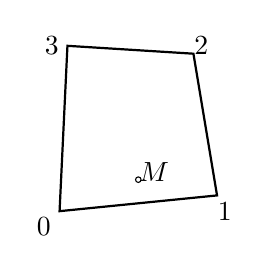
\begin{tikzpicture}
%\draw[step=0.5cm,gray,very thin] (0,0) grid (4,4); %background grid
\draw[thick] (1,1) -- (3,1.2) -- (2.7,3) -- (1.1,3.1) -- cycle;  
\node[] at (0.8,0.8) {0};
\node[] at (3.1,1) {1};
\node[] at (2.8,3.1) {2};
\node[] at (0.9,3.1) {3};
\node[] at (2.2,1.5) {$M$};
\draw (2.,1.4) circle (1pt);
\end{tikzpicture}\\
\end{center}

Several rather simple options exist:
\begin{itemize}
\item we could subdivide the quadrilateral into two triangles and check whether point $M$ is inside any of them (as it turns out, 
this problem is rather straightforward for triangles. Simply google it.)
\item We could check that point $M$ is always on the left side of segments $0\rightarrow 1$, $1\rightarrow 2$, $2\rightarrow 3$, $3\rightarrow 0$.
\item ...  
\end{itemize}

Any of these approaches will work although some might be faster than others. In three-dimensions all will however become 
cumbersome to implement and might not even work at all. Fortunately, there is an elegant way to answer the question, as 
detailed in the following subsection.

%-------------------------------------------
\subsubsection{Three-dimensional space}

If point $M$ is inside the quadrilateral, there exist a set of reduced coordinates $r,s,t\in[-1:1]^3$ such that 

\[
\sum_{i=1}^4 N_i(r_M,s,t) x_i = x_M
\quad\quad\quad
\sum_{i=1}^4 N_i(r_M,s,t) y_i = y_M
\quad\quad\quad
\sum_{i=1}^4 N_i(r_M,s,t) z_i = z_M
\]
This can be cast as a system of three equations and three unknowns. Unfortunately, each shape function $N_i$ 
contains a term $rst$ (as well as $rs$, $rt$, and $st$) so that it is not a linear system and standard techniques
are not applicable. 
We must then use an iterative technique: the algorithm starts with a guess for values $r,s,t$ and 
improves on their value iteration after iteration. 

The classical way of solving nonlinear systems of equations is Newton's method. 
\index{general}{Newton's method}
We can rewrite the equations above as ${\bm F}(r,s,t)=0$:
\begin{eqnarray}
\sum_{i=1}^8 N_i(r,s,t) x_i - x_M&=&0 \nonumber\\
\sum_{i=1}^8 N_i(r,s,t) y_i - y_M&=&0 \nonumber\\
\sum_{i=1}^8 N_i(r,s,t) z_i - z_M&=&0
\end{eqnarray}
or,
\begin{eqnarray}
F_r(r,s,t)&=&0 \nonumber\\
F_s(r,s,t)&=&0 \nonumber\\
F_t(r,s,t)&=&0 \nonumber
\end{eqnarray}

so that we now have to find the zeroes of continuously differentiable functions ${\bm F}:\mathbb{R} \rightarrow \mathbb{R}$.
The recursion is simply:
\[
\left(
\begin{array}{c}
r_{k+1} \\s_{k+1} \\ t_{k+1}
\end{array}
\right)
=
\left(
\begin{array}{c}
r_{k} \\s_{k} \\ t_{k}
\end{array}
\right)
- J_F(r_k,s_k,t_k) ^{-1} 
\left(
\begin{array}{c}
F_r(r_k,s_k,t_k) \\
F_s(r_k,s_k,t_k)\\
F_t(r_k,s_k,t_k)
\end{array}
\right)
\]
where $J$ the Jacobian matrix:
\begin{eqnarray}
J_F(r_k,s_k,t_k)
&=&
\left(
\begin{array}{ccc}
\frac{\partial F_r}{\partial r}(r_k,s_k,t_k) & \frac{\partial F_r}{\partial s}(r_k,s_k,t_k) & \frac{\partial F_r}{\partial t}(r_k,s_k,t_k) \\\\
\frac{\partial F_s}{\partial r}(r_k,s_k,t_k) & \frac{\partial F_s}{\partial s}(r_k,s_k,t_k) & \frac{\partial F_s}{\partial t}(r_k,s_k,t_k) \\\\
\frac{\partial F_t}{\partial r}(r_k,s_k,t_k) & \frac{\partial F_t}{\partial s}(r_k,s_k,t_k) & \frac{\partial F_t}{\partial t}(r_k,s_k,t_k) 
\end{array}
\right) \nonumber\\
&=&
\left(
\begin{array}{ccc}
\sum\limits_{i=1}^8 \frac{\partial N_i}{\partial r}(r_k,s_k,t_k) x_i &
\sum\limits_{i=1}^8 \frac{\partial N_i}{\partial s}(r_k,s_k,t_k) x_i &
\sum\limits_{i=1}^8 \frac{\partial N_i}{\partial t}(r_k,s_k,t_k) x_i \\
\sum\limits_{i=1}^8 \frac{\partial N_i}{\partial r}(r_k,s_k,t_k) y_i &
\sum\limits_{i=1}^8 \frac{\partial N_i}{\partial s}(r_k,s_k,t_k) y_i &
\sum\limits_{i=1}^8 \frac{\partial N_i}{\partial t}(r_k,s_k,t_k) y_i \\
\sum\limits_{i=1}^8 \frac{\partial N_i}{\partial r}(r_k,s_k,t_k) z_i &
\sum\limits_{i=1}^8 \frac{\partial N_i}{\partial s}(r_k,s_k,t_k) z_i &
\sum\limits_{i=1}^8 \frac{\partial N_i}{\partial t}(r_k,s_k,t_k) z_i 
\end{array}
\right) \nonumber 
\end{eqnarray}
In practice, we solve the following system:
\[
J_F(r_k,s_k,t_k) 
\left[  
\left(
\begin{array}{c}
r_{k+1} \\s_{k+1} \\ t_{k+1}
\end{array}
\right)
-
\left(
\begin{array}{c}
r_{k} \\s_{k} \\ t_{k}
\end{array}
\right)
\right]=-
\left(
\begin{array}{c}
F_r(r_k,s_k,t_k) \\
F_s(r_k,s_k,t_k)\\
F_t(r_k,s_k,t_k)
\end{array}
\right)
\]
Finally, the algorithm goes as follows:
\begin{itemize}
\item set guess values for $r,s,t$ (typically 0)
\item loop over k=0,...
\item Compute rhs= $-{\bm F}(r_k,s_k,t_k)$ 
\item Compute matrix $J_F(r_k,s_k,t_k)$
\item solve system for $(dr_k,ds_k,dt_k)$
\item update $r_{k+1}=r_k+dr_k$, $s_{k+1}=s_k+ds_k$, $t_{k+1}=t_k+dt_k$ 
\item stop iterations when $(dr_k,ds_k,dt_k)$ is small
\item if $r_k,s_k,t_k\in[-1,1]^3$ then $M$ is inside.
\end{itemize}
This method converges quickly but involves iterations, and multiple solves of $3\times 3$ systems which, 
when carried out for each marker and at each time step can prove to be expensive. 
A simple modification can be added to the above algorithm: iterations should be carried out {\it only}
when the point $M$ is inside of a cuboid of size $[\min\limits_i{x_i}:\max\limits_i{x_i}]\times[\min\limits_i{y_i}:\max\limits_i{y_i} ]
\times[\min\limits_i{z_i}:\max\limits_i{z_i}]$ where the sums run over the vertices of the element. 
In 2D this translates as follows: only carry out Newton iterations when $M$ is inside the red rectangle!
\begin{center}
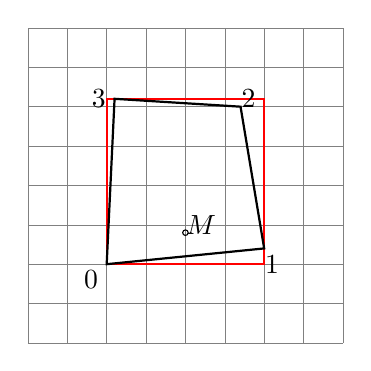
\begin{tikzpicture}
\draw[step=0.5cm,gray,very thin] (0,0) grid (4,4); %background grid
\draw[thick,red] (1,1) -- (3,1) -- (3,3.1) -- (1,3.1) -- cycle;  
\draw[thick] (1,1) -- (3,1.2) -- (2.7,3) -- (1.1,3.1) -- cycle;  
\node[] at (0.8,0.8) {0};
\node[] at (3.1,1) {1};
\node[] at (2.8,3.1) {2};
\node[] at (0.9,3.1) {3};
\node[] at (2.2,1.5) {$M$};
\draw (2.,1.4) circle (1pt);
\end{tikzpicture}\\
\end{center}

Note that the algorithm above extends to high degree elements such as $Q_2$ and higher, even with curved sides.


\todo[inline]{write about case when element is rectangle/cuboid}


 %---------
\newpage %---------------------------------------------------------------------
\subsection{Error measurements and convergence rates} \index{$L_1$ norm}
\index{$L_2$ norm}
\index{$H^1$ norm}

What follows is written in the case of a two-dimensional model. Generalisation to
3D is trivial. What follows is mostly borrowed from \cite{thmk14}.

When measuring the order of accuracy of the primitive variables $\vec{v}$ and $p$,
it is standard to report errors in both the $L_1$ and the $L_2$ norm.
For a scalar quantity $\Psi$, the $L_1$ and $L_2$ norms are computed as
\[
\norm{\Psi}_1 = \int_V |\Psi| dV
\quad\quad
\quad\quad
\norm{\Psi}_2 = \sqrt{ \int_V \Psi^2 dV }
\]
For a vector quantity $\vec{k}=(k_x,k_y)$ in a two-dimensional space,
the $L_1$ and $L_2$ norms are defined as:
\[
\norm{\vec{k}}_1 = \int_V (|k_x|+|k_y|) dV
\quad\quad
\quad\quad
\norm{\vec{k}}_2 = \sqrt{ \int_V (k_x^2+k_y^2) dV }
\]
To compute the respective norms
the integrals in the above norms can be approximated by splitting them
into their element-wise contributions. The element volume integral can then
be easily computed by numerical integration using Gauss-Legendre quadrature.

The respective $L_1$ and $L_2$ norms for the pressure error can be evaluated via
\[
e_p^h|_1 = \sum_{i=1}^{n_e} \sum_{q=1}^{n_q} |e_p^h(\vec{r}_q)| w_q |J_q|
\quad\quad
\quad\quad
e_p^h|_2=\sqrt{ \sum_{i=1}^{n_e} \sum_{q=1}^{n_q} |e_p^h(\vec{r}_q)|^2 w_q |J_q| }
\]
where $e_p^h(\vec{r}_q)=p^h(\vec{r}_q) - p(\vec{r}_q)$ 
is the pressure error evaluated at the $q$-th quadrature associated with
the $i$th element. $n_e$ and $n_q$ refer to the number of elements and
the number of quadrature points per element.
$w_q$ and $J_q$ are the quadrature weight of the Jacobian associated with
point $q$.

The velocity error $e_{\vec v}^h$ is evaluated using the following two norms
\[
e_{\vec{v}}^h|_1 = \sum_{i=1}^{n_e} \sum_{q=1}^{n_q} [ |e_u^h(\vec{r}_q)| + |e_v^h(\vec{r}_q)| ]    w_q |J_q|
\quad\quad
\quad\quad
e_{\vec v}^h|_2=\sqrt{ \sum_{i=1}^{n_e} \sum_{q=1}^{n_q} \left[ |e_u^h({\bm r}_q)|^2 +  e_v^h({\bm r}_q)|^2 \right] w_q |J_q| }
\]
where $e_u^h(\vec{r}_q)=u^h(\vec{r}_q) - u(\vec{r}_q)$ and $e_v^h(\vec{r}_q)=v^h(\vec{r}_q)-v(\vec{r}_q)$.




\index{$H^1(\Omega)$ space} \index{$H^1$ norm} \index{$H^1$ semi-norm}
Another norm is very varely used in the geodynamics literature but is preferred in the 
Finite Element literature: the so-called $H^1$ norm. The mathematical basis for this
norm and the nature of the $H^1(\Omega)$ Hilbert space is to be found in many FE books \cite{dohu03,john16,hugh}.
This norm is expression is expressed as follows for a function $f$ such that $f,|\nabla f|\in L^2(\Omega)$
\footnote{\url{https://en.wikipedia.org/wiki/Sobolev_space}}
\[
\norm{f}_{H^1} = \left( \int_\Omega ( |f|^2 + |\nabla f|^2  ) d\Omega   \right)^{1/2}
\]
We then have 
\[
e_{\vec v}^h|_{H^1} = \norm{\vec{v}^h-\vec{v}}_{H^1} = \sqrt{
\sum\limits_{i=1}^d 
\int_\Omega  
\left[
({v}_i^h-{v}_i)^2
+
\vec\nabla(v_i^h-v_i)\cdot\vec\nabla(v_i^h-v_i) 
\right] d\Omega   
}
\]
where $d$ is the number of dimensions.
Note that sometimes the following semi-norm is used \cite{dobo04,bodg06}:
\[
e_{\vec v}^h|_{H^1} = \norm{\vec{v}^h-\vec{v}}_{H^1} = \sqrt{
\sum\limits_{i=1}^d 
\int_\Omega  
\left[
\vec\nabla(v_i^h-v_i)\cdot\vec\nabla(v_i^h-v_i) 
\right] d\Omega   
}
\]
 

When computing the different error norms for $e_p$ and $e_{\vec v}$ for a set of numerical experiments with
varying resolution $h$ we expect the error norms to follow the following relationships:
\[
e_{\vec v}^h|_1 = C h^{rvL_1} 
\quad\quad\quad\quad
e_{\vec v}^h|_2 = C h^{rvL_2} 
\quad\quad\quad\quad 
e_{\vec v}^h|_{H^1} = C h^{rvH^1}
\]
\[
e_p^h|_1 = C h^{rpL_1} 
\quad\quad\quad 
e_p^h|_2 = C h^{rpL_2}
\]
where $C$ is a resolution-independent constant
and $rpXX$ and $rvXX$ are the convergence rates for
pressure and velocity in various norms, respectively. 
Using linear regression on the logarithm of the respective error norm and the resolution $h$,
one can compute the convergence rates of the numerical solutions.

As mentioned in \cite{dobo04}, when finite element solutions converge at
the same rates as the interpolants we say that the method is optimal, i.e.:
\index{optimal rate}

\[
e_{\vec v}^h|_{L_2} = {\cal O}(h^3)
\quad\quad\quad\quad
e_{\vec v}^h|_{H^1} = {\cal O}(h^2)
\quad\quad\quad\quad
e_{p}^h|_{L_2} = {\cal O}(h^2)
\]

%\begin{itemize}
%\item For $Q_1P_0$, the theoretical lower bound for $r_v'$ is 2 and for $r_p'$ it is 1
%\item For $Q_2P_{-1}$, the theoretical lower bound for $r_v'$ is 3 and for $r_p'$ it is 2
%\end{itemize}
We note that when using discontinuous pressure space
(e.g., $P_0$, $P_{-1}$), these bounds remain valid even
when the viscosity is discontinuous provided that the element boundaries conform to the discontinuity.

 
\subsubsection{About extrapolation}
\index{Extrapolation}

{\it Section contributed by W. Bangerth and part of Thieulot \& Bangerth [in prep.]}

In a number of numerical benchmarks we
want to estimate the error $X_h-X^\ast$ between a quantity $X_h$ computed
from the numerical solution $\vec{u}_h,p_h$ and the corresponding value
$X$ computed from the exact solution $\vec{u},p$. Examples of such quantities
$X$ are the root mean square velocity $v_{rms}$, but it could also be a mass flux
across a boundary, an average horizontal velocity at the top boundary, or
any other scalar quantity.

If the exact solution is known, then one can of course compute $X$ from it.
On the other hand, we would of course like to assess convergence also in
cases where the exact solution is not known. In that case, one can compute
an \textit{estimate} $X^\ast$ for $X$ by way of \textit{extrapolation}.
To this end, we make the assumption that asymptotically, $X_h$ converges to
$X$ at a fixed (but unknown) rate $r$, so that
\begin{equation}
  \label{eq:extrapolation-1}
  e_h=|X_h-X| \approx C h^r.
\end{equation}
Here, $X$, $C$ and $r$ are all unknown constants to be determined, although
we are not really interested in $C$.
We can evaluate $X_h$ from the numerical solution
on successively refined meshes with mesh sizes $h$, $h/2$, and $h/4$. Then,
in addition to \eqref{eq:extrapolation-1} we also have
\begin{eqnarray}
  \label{eq:extrapolation-2}
  e_{h/2}=|X_{h/2}-X| \approx C \left(\frac h2\right)^r,
  \\
  \label{eq:extrapolation-3}
  e_{h/4} =|X_{h/4}-X| \approx C \left(\frac h4\right)^r.
\end{eqnarray}
Taking ratios of equations \eqref{eq:extrapolation-1}--\eqref{eq:extrapolation-3},
and replacing the unknown $X$ by an \textit{estimate} $X^\ast$, we then
arrive at the following equation:
\begin{equation*}
\frac{|X_h-X^\star|}{|X_{h/2}-X^\star|}
=
\frac{|X_{h/2}-X^\star|}{|X_{h/4}-X^\star|}=2^r.
\end{equation*}
If one assumes that $X_h$ converges to $X$ uniformly either from above or
below (rather than oscillate around $X$), then this equation allows us
to solve for $X^\ast$ and $r$:
\begin{equation*}
X^\star = \frac{X_h X_{h/2}-X_{h/2}^2}{X_h - 2 X_{h/2} + X_{h/4}}, \qquad\qquad
r = \log_2 \frac{X_{h/2}-X^\star}{X_{h/4}-X^\star}.
\end{equation*}
In the determination of $r$, we could also have used $X_h$ and $X_{h/2}$,
but using $X_{h/2}$ and $X_{h/4}$ is generally more reliable because
the higher order terms we have omitted in \eqref{eq:extrapolation-1} are less
visible on finer meshes.

 %---------
\newpage %---------------------------------------------------------------------
\subsection{The initial temperature field} \subsubsection{Single layer with imposed temperature b.c.}

Let us take a single layer of material characterised by
a heat capacity $c_p$, a heat conductivity $k$
and a heat production term $H$.

\begin{center}
\includegraphics[width=5cm]{images/initial_temperature/tempcond.png}
\end{center}

The Heat transport equation writes
\[
\rho c_p ( \frac{\partial T}{\partial t} + {\vec v} \cdot {\vec \nabla} { T}) = 
{\vec \nabla} \cdot (k {\vec \nabla} T) + \rho H
\]
At steady state and in the absence of a velocity field, and assuming
that the material properties to be independent of time and space, and that
there is no heat production ($H=0$), this equation
simplifies to
\[
\Delta T =0 
\]
Assuming the layer to be parallel to the $x$-axis, this yields to write
\[
T(x,y)=T(y)=\alpha T+ \beta
\]
In order to specify the constants $\alpha$ and $\beta$, we need two constraints.

At the bottom of the layer $y=y_b$ a temperature $T_b$ is prescribed while a temperature
$T_t$ is prescribed at the top with $y=y_t$. This ultimately yields a temperature field in
the layer given by
\[
\boxed{
T(y) = \frac{T_t-T_b}{y_t-y_b}(y-y_b) + T_b
}
\]

If now the heat production coefficient is not zero, the differential equation
reads
\[
 k \Delta T + H = 0 
\]
The temperature field is then expected to be of the form
\[
T(y)= - \frac{H}{2k} y^2 + \alpha y + \beta 
\]
Supplied again with the same boundary conditions, this leads to
\[
\beta=T_b + \frac{H}{2k} y_b^2 - \alpha y_b
\]
ie,
\[
T(y) = -\frac{H}{2k} (y^2-y_b^2) + \alpha (y-y_b) + T_b
\]
and finally
\[
\alpha =  \frac{T_t-T_b}{y_t-y_b}  + \frac{H}{2k}(y_b+y_t)
\]
or,
\[
T(y) = -\frac{H}{2k} (y^2-y_b^2) + \left( \frac{T_t-T_b}{y_t-y_b}  + \frac{H}{2k}(y_b+y_t)   \right) (y-y_b) + T_b
\]

Taking $H=0$ in this equation obviously yields the temperature field obtained previously.
Taking $k=2.25$, $T_t=0C$, $T_b=550C$, $y_t=660km$, $y_b=630km$ yields the following
temperature profiles and heat fluxes when the heat production $H$ varies:
\begin{center}
\includegraphics[width=5cm]{images/initial_temperature/temperature1.pdf}
\includegraphics[width=5cm]{images/initial_temperature/heatflux1.pdf}
\end{center}
Looking at the values at the top, which are somewhat estimated to be
about $55-65mW/m^2$ \cite[table 8.6]{jama}, one sees that value $H=0.8e-6$ yields a very acceptable
heat flux.
Looking at the bottom, the heat flux is then about $0.03W/m^2$
which is somewhat problematic since the heat flux at the Moho
is reported to be somewhere between 10 and 20 $mW/m^2$ in \cite[table 7.1]{jama}.


%-----------------------------------------------------
\subsection{Single layer with imposed heat flux b.c.}

Let us now assume that heat fluxes are imposed at the top and bottom of the layer:
\begin{center} 
\includegraphics[width=5cm]{images/initial_temperature/tempcond2.png}
\end{center}

We start again from the ODE
\[
k \Delta T + H = 0 
\]
but only integrate it once:
\[
k \frac{dT}{dy}  + H y + \alpha  = 0 
\]
At the bottom $q=k(dT/dy)|_{y=y_b} = q_b$ and at the top
$q=k(dT/dy)|_{y=y_t} = q_t$ so that 

\todo[inline]{to finish}


 
%-----------------------------------------------------
\subsection{Single layer with imposed heat flux and temperature b.c. }

\begin{center}
\includegraphics[width=5cm]{images/initial_temperature/tempcond3.png}
\end{center}

\todo[inline]{to finish}


%---------------------------------------------------------------
\subsubsection{Half cooling space}

%---------------------------------------------------------------
\subsubsection{Plate model}

%---------------------------------------------------------------
\subsubsection{McKenzie slab}










 %-------
\newpage %---------------------------------------------------------------------
\subsection{Kinematic boundary conditions} \index{general}{Essential Boundary Conditions}
\index{general}{Natural Boundary Conditions}

Boundary conditions come in two basic flavors: essential and natural.
\begin{itemize}
\item Essential bcs directly affect DOFs, and are imposed on the FEM matrix. 
\item Natural bcs do not directly affect DOFs and are imposed on the right-hand side vector.
\end{itemize}

\subsubsection{In-out flux boundary conditions for lithospheric models}

\begin{center}
\includegraphics[width=8cm]{images/boundary_conditions/bc1}\\
\includegraphics[width=8cm]{images/boundary_conditions/drawing.png}
\end{center}

The velocity on the side is given by
\begin{eqnarray}
u(y) &=& v_{ext} \quad\quad y<L_1 \nn\\
u(y) &=& \frac{v_{in}-v_{ext}}{y_2-y_1}(y-y_1) + v_{ext} \quad\quad y_1<y<y_2 \nn\\
u(y) &=& v_{in} \quad\quad y>y_2 \nn
\end{eqnarray}
The requirement for volume conservation is:
\[
\Phi=\int_{0}^{L_y} u(y) dy = 0
\]
Having chosen $v_{in}$ (the velocity of the plate), one can then compute $v_{ext}$
as a function of $y_1$ and $y_2$.

\begin{eqnarray}
\Phi
&=&\int_{0}^{y_1} u(y) dy  +\int_{y_1}^{y_2} u(y) dy +\int_{y_2}^{L_y} u(y) dy \nn\\
&=& v_{ext} y_1  + \frac{1}{2}(v_{in}+v_{ext})(y_2-y_1) + (L_y-y_2) v_{in} \nn\\
&=& v_{ext} [y_1 + \frac{1}{2}(y_2-y_1) ] + v_{in} [ \frac{1}{2}(y_2-y_1)  + (L_y-y_2) ] \nn\\
&=& v_{ext}\frac{1}{2} (y_1 + y_2 ) + v_{in} [ L_y - \frac{1}{2}(y_1+y_1) ] \nn
\end{eqnarray}
and finally
\begin{mdframed}[backgroundcolor=blue!5]
\[
v_{ext} = -v_{in} \frac{ L_y - \frac{1}{2}(y_1+y_1)}{ \frac{1}{2} (y_1 + y_2 ) }
\]
\end{mdframed}

Note that in some cases applying free slip boundary conditions on a curved boundary with a triangular mesh 
can be problematic as explained in Dione \etal (2013) \cite{ditu13}.

\Literature \cite{ensg82}
 %--------------
\newpage %---------------------------------------------------------------------
\subsection{Computing gradients - the recovery process} 
write about recovering accurate strain rate components and heat flux components on the nodes.

Let $\vec g(\vec r)$  be the desired nodal 
field which we want to be the continuous $Q_1$ representation of the field $\vec \nabla f^h$.
Since the derivative of the shape function does not exist on the nodes we need to design
an algorithm do do so. This problem is well known and has been 
investigated %\cite{XX.XXX}
\improvement{refs!}.
The main standard techniques are listed hereafter.


%..............................
\subsubsection{Global recovery}

The global recovery approach is rather simple: we wish to find $\vec g^h$
such that it satisfies
\[
\int_\Omega \phi \vec g^h \; d\Omega  = \int_\Omega \phi \vec\nabla f^h \; d\Omega 
\quad\quad \forall \phi
\] 
We will then successively replace $\phi$ by all the shape functions $N_i$ 
and since we have $g^h=\sum_j N_i g_i$ we then obtain
\[
\sum_j \int N_i N_j d\Omega g_i = \int N_i  \vec\nabla f^h \; d\Omega 
\]
or, 
\[
\mathbb{M} \cdot \vec{\cal G} = \vec f
\]



%..................................................
\subsubsection{Local recovery - centroid average over patch}





%..................................................
\subsubsection{Local recovery - nodal average over patch}

Let $j$ be the node at which we want to compute $\vec g$.
Then 
\[
\vec g_j = \vec g(\vec r_j) = 
\frac{\sum\limits_{ e \text{ adj. to }j} |\Omega_e| (\vec\nabla f)_e(\vec r_j) }{\sum |\Omega_e|}
\]
where $|\Omega_e|$ is the volume of the element and $(\vec\nabla f^h)_e(\vec r_j)$
is the gradient of $f$ as obtained with the shape functions inside element $e$ and 
computed at location $\vec r_j$.

%........................................................
\subsubsection{Local recovery - least squares over patch}



%........................................................
\subsubsection{Link to pressure smoothing}

When the penalty method is used to solve the Stokes equation, the pressure
is then given by $p=-\lambda \vec\nabla \cdot \vec v$. As explained in 
section \ref{sec_penalty}, the velocity is first obtained and the pressure 
is recovered by using this equation as a postprocessing step. Since the divergence 
cannot be computed easily at the nodes, the pressure is traditionally computed 
in the middle of the elements, yielding an elemental pressure field (remember, 
we are talking about $Q_1P_0$ elements here -- bi/tri-linear velocity, discontinuous
constant pressure)



\improvement{tie to fieldstone 12}

 %-----
\newpage %---------------------------------------------------------------------
\subsection{Tracking materials and/or interfaces} \begin{flushright} {\tiny {\color{gray} tracking.tex}} \end{flushright}

Unless using a fully Lagrangian formulation, one needs an additional numerical method to represent/track
the various materials present in an undeformable (Eulerian) mesh.
The figure below (by B. Hillebrand) illustrates the three main methods used in geodynamics.

\begin{center}
\includegraphics[width=15cm]{images/tracking/tracking}
\end{center}

Note that what follows is applicable to FEM, FDM, etc ...


A typical test for advection algorithm is the Zalesak disk \cite{zale79}. It is a two dimensional test 
problem of solid body rotation with a constant angular velocity $\omega$ (in rad/sec):

\begin{center}
\includegraphics[width=6cm]{images/tracking/zale79a}
\includegraphics[width=6cm]{images/tracking/zale79b}\\
{\tiny Taken from \cite{zale79}. Left: Schematic representation of two dimensional 
solid body rotation problem. The field inside the cut out has value 3 and it is 1
outside. The rotational speed is such that one full revolution is effected in 
628 cycles. The width of the gap separating the two halves of the cylinder,
as well as the maximum extent of the "bridge" connecting the two halves, is 5 cells.
Right: Perspective view of initial conditions for the two dimensional! solid body rotation
problem. Note that only a $50\times50$ portion of the mesh centered on the cylinder is displayed.}
\end{center}

This benchmark is widely used in the literature \cite{stco91,supu00,vasv05,dilp06,basd08,zhbl14}.
Note that the Zalesak disc is often supplemented with a cone and a Gaussian features:

\begin{center}
\includegraphics[width=6cm]{images/tracking/leve96}\\
{\tiny Taken from \cite{leve96}. Initial data for solid rotation tests}
\end{center}

%..............................................
\subsubsection{The Particle-in-cell technique}\label{ss:pic}
\index{general}{Particle-in-Cell}  
\index{general}{Marker-and-Cell} 
\index{general}{PIC} 
\index{general}{MAC}

\begin{remark}
The terms 'particle' and 'marker' are commonly (and unfortunately) interchangeably used in the literature 
in the context of the particle-in-cell technique. However, one should be aware that the marker-and-cell (MAC) 
technique is something different: it was invented in the early 60's at the Los Alamos Laboratories by 
Harlow and Welch (1965) \cite{hawe65}. For more information on MAC see the review paper 
by McKee \etal (2008) \cite{mctf08}. 
Also, Tackley and King (2003) \cite{taki03} talk about the tracer-ratio method in the context of PIC... 
\end{remark}

The Particle-in-cell method is by far the most widely used in computational geodynamics. 
In its most basic form it is a rather simple method to implement and this probably owes to its success
and early adoption \cite{popo92}  in non-parallel codes such as \sopale \cite{full95}, 
I2VIS \cite{geyu03} or \citcoms \cite{mczh04} (Appendix~\ref{app:codes}).
It has been implemented in \aspect{} \cite{galh18} and the inherent load balancing issues arising from the 
parallel implementation as well as from the use of Adaptive Mesh Refinement are discussed. 
It has also been implemented in the MILAMIN code \cite{daks08} to study LLSVPs \cite{musd15}.

\begin{center}
\includegraphics[width=8cm]{images/tracking/crsg12}\\
{\captionfont One of the main problems of the PIC method is the fact that the interface 
between the fluid is not tracked explicitely, and if one uses a random distribution of 
particles the black dotted line reprensents the 'real' interface between the fluids 
while the red line is liekly to be the interface one would obtain based on the 
distribution of particles. Taken from Crameri \etal (2012) \cite{crsg12}.}
\end{center}

Samuel (2018) \cite{samu18} does a great job at explaining 
the core problem with PIC: {\it the method requires the method requires particle-mesh 
and mesh-particle mappings to be specified. These critical operations constitute a
major source of inaccuracy in the PIC solution \cite{mona85,dumg11,thmk14}. 
Indeed, while the Lagrangian advection alone is not prone
to significant numerical diffusion, particle–mesh mappings can introduce 
important amounts of dissipation. This is particularly true
when the spatial distribution of particles is not homogeneous, leading 
to areas in the vicinity of gridpoints that are not sufficiently
well sampled by particles, and other regions where the domain is
oversampled by particles. This recurrent sampling problem develops 
in regions characterized by strong deformation, and concerns
both compressible and incompressible flow \cite{waav15,pukp16}. 
The non-homogeneous sampling has two main
origins. \\
- The first one corresponds to inaccuracies in advecting the
Lagrangian particles \cite{meje04}. This aspect has drawn
the attention of a few recent studies \cite{waav15,pukp16}, 
which have proposed the use of conservative schemes to
map velocity components from the Eulerian grid to the Lagrangian
particles during their advection. Such schemes have shown to significantly 
improve the accuracy of the interpolation, and result in
a considerably more homogeneous spatial sampling. \\
- The second origin, which has received less attention, is related to the deforming
nature of the flow \cite{modm03}, and is completely independent 
of the accuracy of the numerical methods for interpolating
the velocities at particles’ locations. In fact, for a given velocity
field, particles should travel along their characteristics, and even in
the case of incompressible flows, the distance between characteristics 
can vary in general, and can strongly diverge or converge in
regions characterized by strong deformation. This naturally leads to
the development of a non-homogeneous spatial distribution of the
Lagrangian particles, even if the particles locations are perfectly
known.}



The basic methodology goes as follows:
\begin{enumerate}
\item distribute particles in the domain
\item assign a material identity (and/or any other quantity) to each of them
\item project particle quantities of the Eulerian nodes of the mesh
\item solve the Stokes equations for a new velocity field
\item interpolate the velocity onto the particles
\item move the particles with their respective velocities 
\item go back to step 3
\end{enumerate}  

As it turns out each step above needs to be carefully executed and is more difficult than it 
first looks. 

\paragraph{Distributing particles in the domain}. Let us assume we wish to distribute $N_p$ particles
in the domain. How large must $N_p$ be? To simplify, one end member could be 'as many particles as possible that fit in memory' 
while the other end member could be 'one per element/cell on average'. While the former does not necessarily guarantee a 
desired accuracy while being CPU and memory intensive, the latter will certainly lead to zones in the domain void 
of particles which will be problematic since the projection onto the mesh might yield zero values or very inaccurate values.
How many particles (per element/cell) will be enough?
Also, should the particles be randomly distributed in the domain or on some kind of regular grid? 
See \stone 13.

Taken from Tackley and King (2003) \cite{taki03}: "Tracers are initialized on a regular grid 
with each tracer perturbed from its grid position by a random amount of up to
$\pm$ half a grid spacing, in order to eliminate artifacts due to tracer alignment."


\paragraph{Averaging and projection}. This is a very critical step. Unfortunately, there is no community-wide
agreed-upon method. The problem at hand boils down to: at a given location $(\vec r)$ in space I need a
the value of a field which is carried by the particles. 
The first step is to find the particle(s) close to this point. If done naively, this is a very costly affair, 
and begs the question what 'close' means. Finding all particles within a radius $R$ of point $\vec r$ can 
be done very efficiently (e.g. with linked lists, Verlet lists, ...) but the choice 
of $R$ proves to be critical:
if too small, there may not be any particle inside the circle, and if too large there may be many particles 
inside the circle and the averaging over so many particles in space will prove to be over diffusive. 
In practice, the FD or FE mesh is used to provide an indication of $R$. 
In FDM, the four cells (or quarter cells) around
a node represent the volume of space containing the particles whose properties are to be averaged \cite{dumg11} 
as illustrated in the following figure:

\begin{center}
\includegraphics[width=12cm]{images/dumg11}\\
{\captionfont Taken from \cite{dumg11}. The "4-cell" and "1-cell" schemes for projecting 
properties defined on the markers (denoted by stars) onto a node (denoted by the solid circle). 
(A) The 4-cell scheme. The support of the interpolating function $N_i$ associated
with node $i$ is indicated by the shaded region. Only markers within the support of node $i$ 
contribute to the projection operation used to define the nodal value at $i$. The shape of 
the bilinear interpolation function for node $i$ is indicated in the lower frame. 
(B) The 1-cell scheme. The thick lines in the lower frame indicate the grid used to discretize the
Stokes equations, while the thin lines indicate the grid onto which marker properties are projected. 
The 1-cell scheme utilizes a compact support of size $\Delta x \times  \Delta y$. The support 
for nodes $r$, $s$, $t$ are indicated by the shaded regions. Only markers within the nodal 
support contribute to the projection operation for that node.}
\end{center}

Given that the FEM requires to compute integrals over each element, one could assume that 
only the particles inside the element will contribute 
to the average values assigned to the quadrature points (which I coin 'elemental approach'). 

However, one could also decide to first average the properties onto the nodes
before using these nodal values to assign values to the quadrature points (which I coin 'nodal approach'). 
In this case the FDM approach seen above could apply. 

Finally, in both FDM and FEM bi/trilinear basis functions are used for the interpolation as 
they can be interpreted as weighing functions. Higher order basis functions could also be used 
but the standard $Q_2$ basis functions (Section~\ref{sec:shpfct2d})
are 2-nd order polynomials which can take negative values (as opposed to the $Q_1$ 
basis functions which are strictly positive)
and this can pose problems: in some cases, although all values to be averaged are positive, 
their weighed average can be negative.
See Section~\ref{ss:bern} for concrete examples.

\underline{nodal approach}

\underline{elemental approach (1) - piece-wise constant interpolation} 

What follows is written with simplicity in mind, although more mathematical formulations 
can be found in the literature \cite{galh18}.

Assuming that we have established a list of particles tracking a field $f(\vec r)$ inside the 
element 
%and that each particle has an 
%associated weight $w_i$ (function of the location where the average is to be computed or not), 
we must now compute their average value $<f>$. 
The simplest approach which comes to mind is the arithmetic mean ($am$):
\[
\langle f\rangle_{am} = \frac{\sum\limits_{i=1}^n f_i}{n}
\]  
where $n$ is the number of particles inside the element.
In the case where $f$ is the (mass) density $\rho$, it is indeed what should be used. 
However, turning now to viscosity $\eta$, we know that its value can vary by many orders of magnitude 
over very short distances.
It is then likely that the average runs over values spanning values between 
$10^{18}\text{Pa s}$ and $10^{25} \text{Pa s}$.
As explained in \cite{scbe08} the arithmetic averaging tends to 'favour' large values: 
if the sum runs over 
10 particles, 9 carrying the value $10^{25}$ and 1 carrying the value $10^{19}$, 
the average value is then
\[
\langle\eta\rangle = \frac{9\cdot 10^{25}+1\cdot 10^{19}}{10} \simeq 0.9\cdot 10^{25}
\]
which is much much closer to $10^{25}$ than to $10^{19}$.
Other averagings are then commonly used, namely the geometric mean ($gm$)  and the 
harmonic mean ($hm$), defined as follows:
\[
\langle f\rangle_{gm} = \left( \prod_i f_i \right)^{1/n} 
\qquad
\text{or, }
\qquad
\log_{10} \langle f \rangle_{gm} = \frac{\sum\limits_{i=1}^{n} \log_{10} f_i }{n}  
\]
and 
\[
\langle f\rangle_{hm} = \left( \frac{\sum\limits_{i=1}^n \frac{1}{f_i} }{n}  \right)^{-1}
\qquad
\text{or, }
\qquad
\frac{1}{\langle f\rangle_{hm} } = \frac{\sum\limits_{i=1}^n  \frac{1}{f_i} }{n}  
\]
The geometric mean can be seen as a form of arithmetic mean of $\log_{10}$ values, 
while the harmonic mean can be seen as 
a form of arithmetic mean of the inverse values.

Looking back at the above example, the geometric mean of the viscosities is given by 
\[
\log \langle \eta\rangle_{gm} = \frac{9\cdot 25+1\cdot 19}{10} = 24.4 
\qquad \text{or,} \qquad 
\langle \eta\rangle_{gm} \simeq 2.5 \cdot 10^{24}
\]
and the harmonic mean:
\[
\langle\eta\rangle_{hm} \simeq \left( \frac{1}{10 \cdot  10^{19}} \right)^{-1} = 10^{20}
\]
We see that the harmonic mean tends to favour the small values. Also we recover the known property:
\begin{equation}
\langle f \rangle_{am}\quad  \geq \quad
\langle f \rangle_{gm}\quad  \geq \quad
\langle f \rangle_{hm} 
\end{equation}

%When all $f_i$ are equal to $f_0$ their computed average should also be equal to $f_0$. As a consequence the 
%weights $N_i$ should fulfil the condition $\sum\limits_{i=1}^n N_i=1$.
%If all weights are equal, then $N_i=1/n$ and the averagings become:

%\begin{equation}
%\langle f\rangle_{am} = \frac{1}{n} \sum\limits_{i=1}^n f_i
%\qquad
%\langle f\rangle_{gm} = \prod_i f_i^{1/n} 
%\qquad
%\langle f\rangle_{hm} = \left( \frac{1}{n}\sum_i^n \frac{1}{\phi_i} \right)^{-1}
%\end{equation}

Once a single average value has been computed for the whole element, then 
all quadrature points are assigned this value. 


\underline{elemental approach (2) - Least Squares Interpolation } 
One can revisit this topic on the grounds that 
with high(er) order elements optimal convergence is unlikely to be reached 
if viscosity (and density) are assumed to be constant inside each element (see  
\cite{galb19}). One could therefore use the least-square method to arrive at 
a functional representation of the field inside the element which is as 
close as possible (in the least-squares sense, then) to the particle-based field. 

Thielmann \etal (2014) \cite{thmk14} use the $Q_2P_{-1}$ element and introduce an element-wise interpolation
scheme based on a least squares fitting of the particle properties and choose the functional to 
be a linear function to match the pressure space. 
They define the error $\epsilon$ such that 
\[
\epsilon^2 = \sum_{i=1}^n ( \tilde{f}(x_i,y_i)-f_i)^2
\]
with $\tilde{f}(x,y)=a+bx+cy$. 
We then look for the minimum of $\epsilon^2$, i.e. $\vec\nabla(\epsilon^2)=0$ in the $\{a,b,c\}$ space.
So 
\begin{eqnarray}
0=\frac{\partial \epsilon^2}{\partial a} 
&=& 2\sum\limits_i ( \tilde{f}(x_i,y_i)-f_i) \nn\\
&=& 2\sum\limits_i ( a + bx_i +cy_i -f_i) \nn\\
&=& 2 \left[ a \sum\limits_i 1 + b \sum\limits_i x_i + c \sum y_i - \sum\limits_i f_i \right] \nn\\
0=\frac{\partial \epsilon^2}{\partial b} &=& 2\sum\limits_i ( \tilde{f}(x_i,y_i)-f_i) x_i \nn\\
&=& 2\sum\limits_i ( a + bx_i +cy_i -f_i) x_i \nn\\
&=& 2 \left[ a \sum\limits_i x_i  + b \sum\limits_i x_i^2 + c \sum x_i y_i - \sum\limits_i x_i f_i \right]\nn\\
0=\frac{\partial \epsilon^2}{\partial c} &=& 2\sum\limits_i ( \tilde{f}(x_i,y_i)-f_i) y_i \nn\\ 
&=& 2\sum\limits_i ( a + bx_i +cy_i -f_i) y_i \nn\\
&=& 2 \left[ a \sum\limits_i y_i + b \sum\limits_i x_i y_i + c \sum y_i^2 - \sum\limits_i y_if_i \right] \nn
\end{eqnarray}
so 
\[
\left( 
\begin{array}{ccc}
\sum\limits_i 1 & \sum\limits_i x_i & \sum\limits_i y_i \\
\sum\limits_i x_i & \sum\limits_i x_i^2 & \sum\limits_i x_iy_i \\
\sum\limits_i y_i & \sum\limits_i x_i y_i & \sum\limits_i y_i^2 
\end{array}
\right)
\cdot
\left(
\begin{array}{c}
a\\
b\\
c
\end{array}
\right)
=
\left(
\begin{array}{c}
\sum\limits_i f_i \\
\sum\limits_i x_i f_i \\
\sum\limits_i y_i f_i 
\end{array}
\right)
\]

We could also then decide to use a bi-linear function $\tilde{f}$, i.e.
\[
\tilde{f}(x,y)=a+bx+cy+dxy
\]
which lies in the $Q_1$ space of Taylor-Hood quadrilateral elements. In this case the error is 
\[
\epsilon^2 
= \sum_{i=1}^n ( \tilde{f}(x_i,y_i)-f_i)^2
= \sum_{i=1}^n (a+bx_i+cy_i + dx_iy_i -f_i)^2
\]
and one has to solve a $4\times 4$ system this time:
\[
\left( 
\begin{array}{cccc}
\sum\limits_i 1 & \sum\limits_i x_i & \sum\limits_i y_i & \sum\limits_i x_iy_i\\
\sum\limits_i x_i & \sum\limits_i x_i^2 & \sum\limits_i x_iy_i & \sum\limits_i x_i^2 y_i\\
\sum\limits_i y_i & \sum\limits_i x_i y_i & \sum\limits_i y_i^2 & \sum\limits_i x_iy_i^2\\ 
\sum\limits_i x_iy_i & \sum\limits_i x_i y_i & \sum\limits_i y_i^2 & \sum\limits_i x_i^2y_i^2  
\end{array}
\right)
\cdot
\left(
\begin{array}{c}
a\\
b\\
c\\
d
\end{array}
\right)
=
\left(
\begin{array}{c}
\sum\limits_i f_i \\
\sum\limits_i x_i f_i \\
\sum\limits_i y_i f_i \\
\sum\limits_i x_i y_i f_i 
\end{array}
\right)
\]


Once this linear system (or the previous one) has been solved we have obtained the coefficients $a,b,c(,d)$ 
which allow us to compute $\tilde{f}$ anywhere inside the element, and especially 
at the quadrature points. 

\begin{remark}
Using a different (bi)linear function $\tilde{f}$ for each element 
means that it is likely to be discontinuous 
from one element to another in regions of high gradients. 
\end{remark}

There is however one drawback with this approach (linear or bi-linear alike):
in the areas of steep gradients the computed coefficients can be such that 
the function $\tilde{f}$ evaluated on a quadrature point 
is negative  which 1) would be wrong but not numerically 
dramatic for density, 2) would be wrong and physically and numerically 
problematic for viscosity (a viscosity cannot be negative, and this would 
automatically destroy the SPD nature of the viscous block of the Stokes matrix).

This problem is discussed in Thielmann \etal (2014) in Section 3.2.1 and they 
call this "Over- and Under-shooting". A simple (iteratuve) 
fix is then designed which insures that the computed value is within user-defined 
acceptable bounds. This is also mentioned in \cite{galb19} but the authors 
explain that this problem was not encountered in the context of the publication.





\begin{remark}
Two variants of the PIC methods have been proposed: the Deformable PIC (DPIC) 
by Samuel (2018) \cite{samu18}, and the multiscale PIC in \cite{asmo12}.
\end{remark}

\begin{remark}
TO BE WRITTEN.
A word about the tracer ratio method. \cite{taki03}. 
Trim \etal (2020) show a modified method 
with a tracer repositioning algorithm designed to promote even tracer
coverage \cite{trlb20}. 
\end{remark}



See Stone~67 for a concrete example of Particle-In-Cell use and a detailed 
explanation of its implementation.



%.....................................................................
\paragraph{Interpolation of the velocity onto particles}.

Once the particle $i$ has been localised inside a given element (Section~\ref{sec:amiin}) 
and its reduced coordinates $(r,s,t)$ determined, the velocity at this location can 
be computed through the basis functions:
\[
\vec\upnu_i=\sum_{k=1}^m N_i(r,s,t) \vec\upnu_k
\]
This approach is not without problem: while the nodal velocities $\vec\upnu_k$ are such 
that\footnote{for incompressible flows, of course} 
$\vec\nabla\cdot\vec\upnu=0$ (in the weak sense), the computed velocity $\vec\upnu_i$ 
is not necessarily divergence-free! In order to remedy this, a 
Conservative Velocity Interpolation (CVI) has been proposed in \cite{waav15}.
Because the complete derivations for the CVI algorithm is quite large I 
have decided to make a new section about it (Section~\ref{sec:cvi}) rather than include it 
here.

%.....................................................................
\paragraph{Moving the particles}

This is discussed in the context of the Runge-Kutta Methods, see Section~\ref{sec:rkparticles}.



%..............................................
\subsubsection{The level set function technique}
\index{general}{Level-set Method} 
\index{general}{Level-set Function} 
\index{general}{LSM} 
\index{general}{LSF} 
\index{general}{ENO}

This method was developed in the 80's by Stanley Osher and James Sethian \cite{lofo06}

The Level-set Method (LSM), as it is commonly used in Computational Fluid Dynamics -- and especially 
in Computational Geodynamics -- represents a close curve $\Gamma$ (say, in our case, the 
interface between two fluids or layers) by means of a function $\phi$ (called the level-set function, or LSF).
$\Gamma$ is then the zero level-set of $\phi$:
\begin{equation}
\Gamma = \left\{ (x,y) \; |\; \phi(x,y)=0 \right\}
\end{equation}
The convention is that $\phi>0$ inside the region delimited by $\Gamma$ and $\phi<0$ outside.
The function value indicates on which side of the
interface a point is located (negative or positive) and this is
used to identify materials. 

Furthermore, if the curve $\Gamma$ moves with a velocity $\vec \upnu$, 
then it satisfies the following equation:
\begin{equation}
\frac{\partial \phi}{\partial t} + \vec\upnu \cdot \vec\nabla \phi = 0 
\end{equation}

The level set function is generally chosen to
be a signed distance function, i.e. $|\vec\nabla \phi| = 1$ everywhere 
and its value is also the distance to the interface.

As explained in \cite{hitg14}, the level-set function $\phi$ is advected 
with the velocity $\vec\upnu$ which is obtained by solving the Stokes equations.
This velocity does not guarantee that after an advection step the signed 
distance quality of the LSF is preserved. 
The LSF then needs to be corrected, which is also called reinitialisation. 
Finally, solving the advection equation must be done in an accurate manner both in time and space,
so that so-called ENO (essentially non-oscillatory) schemes are often employed for the 
space derivative \cite{ossh91,saev10}.


The level set method has not often been used in the geodynamics 
community with some notable exceptions 
\cite{bomh06,bomh07,habm07,grbh07,zlfd08,hagr10,sunh10,suhe10,hitg14}
An overview of the method and applications can
be found in \cite{osfe01}.

Several improvements upon the original LSM have been proposed, 
such as for instance the conservative level set of \cite{zhbl14}.
The most notable difference between CLS method originally proposed by Olsson \etal \cite{olkr05,olkz07}
and standard LS method lies in the choice of LS function. Instead of the signed distance function, the
CLS methods employ the Heaviside function $H(\phi)$ 
\[
H(\phi)=
\left\{
\begin{array}{ll}
1 & \phi>0 \\
1/2 & \phi=0 \\
0 & \phi<0
\end{array}
\right.
\]
where $\phi$ is the signed distance function as in the LSM. 
In practice, a hyperbolic tangent function is used:
\[
H(\phi) = \frac{1}{2} (1+\tan (\phi/2\epsilon))
\]
where $\epsilon$ defines the spreading width of $H$. In the case where there are only 
two fluids (i.e. a single level set is sufficient), the material properties such as density and viscosity
are computed as follows:
\[
\rho=\rho_1+(\rho_2-\rho_1)H(\phi)
\]
\[
\eta=\eta_1+(\eta_2-\eta_1)H(\phi)
\]

\Literature: \cite{vasv05,vasv08,migi07,vasv05b}. 
\begin{itemize}
\item Review of level-set methods \cite{gifo18}
\item Interactive 3-D computation of fault surfaces using level sets \cite{kadt08}
\end{itemize}

%..............................................
\subsubsection{The field/composition technique \label{sec:compfield}}
\index{general}{Compositional Field}

This is the approach taken by the \aspect{} developers \cite{krhb12,hedg17}. 
Each material $i$ is represented by a compositional field $c_i$, 
which takes values between 0 and 1.
Each compositional field is then advected with the (prescribed or computed) Stokes velocity \cite{chri92}:
\begin{equation}
\frac{\partial c_i}{\partial t} + {\bm v}\cdot {\bm \nabla }c_i = 0
\end{equation}
The value at a point (Finite element node or quadrature point) is 1 if it is in the 
domain covered by the material $i$, and 0 otherwise.
In one dimension, each compositional field is a Heavyside function. 
This approach is somewhat similar to the LSM but the field is essentially 
discontinuous across the interface, which makes it very difficult to advect.  
On the plus side, compositional fields need not be reinitialised, as opposed to LSF's.

Accurate numerical advection is a notoriously difficult problem. Unless very specialised 
techniques are used it often yields undershoot ($c_i<0$) and overshoot ($c_i>0$), which 
ultimately yields mass conservation issues. Also, unless special care is taken, 
compositional fields tend to become more and more diffuse over time: the SUPG method (Section~\ref{sec:supg})
and the entropy viscosity method \cite{krhb12,ropu19} add small amounts of diffusion to dampen the under- and 
overshoots. This means that at a given point two or more compositions may have values, 
which require some form of averaging. If under- and overshoots are present, these averagings
can become very problematic and even yield meaningless quantities (e.g. negative viscosities).

One rather old and popular filtering approach is the so-called Lenardic and Kaula (1993) \cite{leka93}
filter:

\begin{center}
\includegraphics[width=6cm]{images/compositions/leka93_filter1}\\
\includegraphics[width=6cm]{images/compositions/leka93_filter2}\\
{\captionfont Taken from Lenardic and Kaula \cite{leka93}}
\end{center}

\begin{center}
\includegraphics[width=16cm]{images/compositions/leka93_filter3}\\
{\captionfont From FENICS book}
\end{center}


\begin{center}
\includegraphics[width=8cm]{images/compositions/plth13}\\
{\captionfont 
Filtering approach proposed by Lenardic and Kaula (1993). 
The composition field $C$ is assumed to vary between 0 and 1. Grid points with $C$-values 
lower than 0 and greater than 1 are set to 0 and 1, respectively (red). 
$C_{min}$ and $C_{max}$ are the minimum and maximum spurious values observed. 
Grid points whose $C$-value is lower than $|C_{min}|$ or greater than ($2-C_{max}$) 
are also set to 0 and 1, respectively (blue). 
The $C$-value of all grid points that do not exhibit spurious oscillations (green) is then corrected
according to the difference between the original average composition and that computed after the reset-
ting of the spurious values.
Taken from Plesa \etal (2013) \cite{plth13}.}
\end{center}











\Literature: \cite{vyrc13}

Entropy viscosity method \cite{gupa11}

\improvement[inline]{write about DG approach}






%..............................................
\subsubsection{The Volume-of-Fluid method} 
\index{general}{Volume-of-Fluid Method}
\index{general}{VOF}

%from Napoleon \etal
The Volume-Of-Fluid (VOF) method is a fixed-grid approach based on the one-fluid model and considers that the various immiscible fluids (or `phases') can be described as a single fluid whose local physical properties, namely density and viscosity, vary in space and time depending on the volume fraction $C_i$ of each phase $i$ 
\cite{hini81,youn82}. 

The volume fraction of each fluid intrinsically obeys $\sum \limits_{{i=1}}^n C_i = 1$ where $n$ is the number of phases. 
Typically, $C_i=1$ in grid cells filled only with fluid $i$, and $0<C_i<1$ in grid cells cross--cut by an interface. 
There are two main classes of VOF methods: methods that try to reconstruct exactly the interface between fluids (e.g. \cite{puth18}), which requires significant computational time, and methods that do not, such as in JADIM and OpenFOAM. 
With no interface reconstruction, the thickness of the interfacial region is defined by $0<C_i<1$, and typically occupies two to three grid cells. 

\cite{hini81}\cite{ropu19}

See review of the method in Robey's phd thesis \cite{robe19}.


%..............................................
\subsubsection{The method of characteristics}

\todo[inline]{ask Arie to write something}

\cite{devv00a}

%.............................................
\subsubsection{The Marker Chain method}
\index{general}{Marker Chain method} 

In two dimensions, the idea is quite simple: each interface is discretised by means of a number
of Lagrangian points (which may or may not vary in time). The points are numbered and 
connected (think of the connectivity array of a 1D FEM code). In the case of small deformations, 
and in the absence of in/out-flow boundaries, the method is reasonably trivial to implement, and 
each couple of point defines a segment (and therefore its normal vector too) which can then be used
to answer the question: "at this location, am I above or below this interface" or "am I this domain our
outside this domain" (in the case that the interface does not reach any of the boundaries).

This method becomes somewhat impractical when large deformation occurs or, for example, 
when a domain splits into two (e.g. slab break off). One interface must then become two, 
and it requires an algorithm capable of detecting the breakup of the surface and capable 
of rebuilding/patching the new ones so that they can still be used further. 
Note that in case of large deformation some markers may get further and further apart 
from each other which makes for a poor representation of the surface. New markers should then 
be added but the question of when and where must then be addressed.

Also, switching to three dimensions can prove to be very difficult or simply very 
costly: the generation of the inital marker position is trivial but their connectivity 
can be complicated to establish at startup: for instance, a Stokes sphere will require
a mesh made of triangles which maps exactly the surface of the sphere (see \cite{thie18,moma19} 
for methods on how to efficiently produce such meshes). In the case of more complex 3D geometries
this may prove nearly impossible to do. So will the problem of splitting a surface into two 
(or merging two domains). \todo{I still have pics from the old days using \douar- include} 

This method is usually coupled to Eulerian meshes (typically with FDM, but not only). 
It was used in \cite{woid78} in the context of salt domes analysis and later in \cite{chri82,chyu84}.
It is also used in \cite{vaks97} but little details are given about the algorithms used
to track and update the chain in the presence of such large deformation.
It is also used (athough coupled to level set functions) in the \douar code\cite{brtf08} 
(see Section~\ref{app:codes}). Having worked myself on this code and having had to produce 
complex initial triangulated surfaces for simulations (see for example \cite{lobh10}) it is 
easy to understand why later users of this code did implement the marker-in-cell technique.
More recently, it is used to track the free surface position in a FDM code \cite{dumy16,chmd19}.

Finally, Christensen \cite{chri92} makes the following interesting comment:  
"One might assume that different methods 
of representing the discontinuity, for example, by a tracer chain \cite{chyu84} or a cloud of 
tracers, would solve these problems. However, the difficulties 
arise not only from the way in which material boundaries are 
represented. Physically, the rate of shear strain parallel to a 
rheological boundary is discontinuous. Within the finite ele-
ment scheme such jump can only be realized at an element 
boundary. In an Eulerian scheme, where the discontinuity will 
crosscut the elements, the jump in strain rate must be approx- 
imated by a continuous variation, and effectively, the rheolog-
ical properties on both sides of the discontinuity will be 
averaged in some way within the element."

Literature: Lin \& van Keken (2006) \cite{liva05,liva06a,liva06b,kaus05,mulyukova}

%..............................................
\subsubsection{Hybrid methods}

In Braun \etal \cite{brtf08} a level set method is presented which is based on a 3-D set
of triangulated points, which makes it a hybrid between tracers and level set functions:
in the \douar code (Appendix~\ref{app:codes}) the interface is then explicitely tracked by means of the tracers while the LSF is computed 
on the FE nodes. Although very promising in theory, this method proved to be difficult to use in practice
since it requires a) a triangulation of the interfaces at $t=0$ which is not trivial if the geometries
are complex (think about a slab in 3D); b) the addition or removal of tracers because of the interface deformation
and the patching of the triangulation; c) the calculation of the distance to the interfaces for each 
FE node based on the triangle normal vectors. 
This probably explains why the Particle-In-Cell method was later implemented in this code (pers. comm.).
Note that another very similar approach is used in \cite{saev10}.



%..............................................
\subsubsection{Boundary fitted mesh}

This method is rather simple to implement and works well for small deformations. It is 
for instance used by Frehner \cite{freh14} (see online supplementary material) in which it is 
stated: "The numerical grid is set up in such a way that the interface
between different material phases (two layers in this case) coincides with element boundaries. Hence, each
element belongs to a unique material phase and no interpolation is necessary."
With such a method, each element is initally attributed a material phase/number and its material
properties do not change. 


\vspace{2cm} 

\Literature: three-dimensional front tracking method using a triangular mesh \cite{sclo03}.







 %-----------
\newpage %---------------------------------------------------------------------
\subsection{Static condensation} \index{general}{Static Condensation}

The idea behind static condensation is quite simple: in some cases, there are dofs 
belonging to an element which only belong to that element. For instance, the so-called MINI 
element ($P_1^+ \times P_1$) showcases a bubble function in the middle (see section \ref{ss:pair}). 
In the following, $\vec{\cal V}^\star$ corresponds to the list of such dofs inside an element.
The discretised Stokes equations on any element looks like:

\begin{equation}
\left(
\begin{array}{ccc}
\K   & L & \G \\
L^T & \K^\star  & H \\
\G^T & H^T & 0
\end{array}
\right)_e
\left(
\begin{array}{c}
\vec{\cal V} \\ \vec{\cal V}^\star \\ \vec{\cal P}
\end{array}
\right)_e
=
\left(
\begin{array}{c}
\vec{f} \\ \vec{f}^\star \\ \vec{h}
\end{array}
\right)_e
\end{equation}
This is only a re-writing of the elemental Stokes matrix where the matrix $\K$ has been 
split in four parts.
Note that the matrix $\K^\star$ is diagonal.\todo{check}

This can also be re-written in non-matrix form:
\begin{eqnarray}
\K \cdot \vec{\cal V} + L \cdot \vec{\cal V}^\star + \G \cdot \vec{\cal P} &=& \vec{f} \\
L^T V + K^\star \cdot  \vec{\cal V}^\star + H \cdot \vec{\cal P} &=& \vec{f}^\star \\
\G^T \cdot \vec{\cal V} + H^T \vec{\cal V}^\star &=& \vec{h}
\end{eqnarray}
The $\vec{\cal V}^\star$ in the second equation can be isolated:
\[
\vec{\cal V}^\star = \K^{-\star} \cdot ( \vec{f}^\star - L^T \cdot \vec{\cal V} - H \cdot \vec{\cal P})
\]
and inserted in the first and third equations:
\begin{eqnarray}
\K \cdot \vec{\cal V} + L \left[ \K^{-\star} ( \vec{f}^\star - L^T \cdot \vec{\cal V} - H \cdot \vec{\cal P} )  \right] + \G \cdot \vec{\cal P} &=& \vec{f} \\
\G^T \cdot \vec{\cal V} + H^T \left[  \K^{-\star} ( \vec{f}^\star - L^T \cdot \vec{\cal V} - H \cdot \vec{\cal P}) \right]  &=& \vec{h}
\end{eqnarray}
or,
\begin{eqnarray}
(\K-L\cdot \K^{-\star} \cdot L^T)\cdot \vec{\cal V} + (G-L\cdot \K^{-\star} \cdot H) \cdot \vec{\cal P} &=& \vec{f}-L\cdot \K^{-\star} \cdot \vec{f}^\star \\
(G^T -H^T\cdot \K^{-\star}\cdot  L^T ) \cdot \vec{\cal V}  - 
(H^T \cdot \K^{-\star} \cdot H )\cdot \vec{\cal P}   &=& \vec{h} -H^T\cdot \K^{-\star}\cdot \vec{f}^\star
\end{eqnarray}
i.e.
\begin{eqnarray}
\underline{\K} \cdot \vec{\cal V} + \underline{\G}\cdot \vec{\cal P} &=& \underline{\vec{f}} \\
\underline{\G}^T \cdot \vec{\cal V} - \underline{\C} \cdot \vec{\cal P} &=& \underline{\vec{h}}
\end{eqnarray}
with
\begin{eqnarray}
\underline{\K}&=& K-L\cdot \K^{-\star} \cdot L^T \\
\underline{\G}&=& G-L\cdot \K^{-\star} \cdot H \\
\underline{\C}&=& H^T \cdot \K^{-\star} \cdot H \\
\underline{\vec{f}}&=& \vec{f}-L\cdot \K^{-\star} \cdot \vec{f}^\star \\
\underline{\vec{h}}&=& \vec{h} -H^T\cdot \K^{-\star}\cdot \vec{f}^\star
\end{eqnarray}
Note that $\underline{\K}$ is symmetric, and so is the Stokes matrix.


For instance, in the case of the MINI element, the dofs corresponding to the bubble 
could be eliminated at the elemental level, which would make the Stokes matrix smaller
(see book by Braess \cite{braess}). 
However, it is then important to note that static condensation introduces a 
pressure-pressure term which was not there in the original formulation.









 %-----------------
\newpage %---------------------------------------------------------------------
\subsection{Measuring incompressibility \label{ss_incomp}} 
The velocity divergence error integrated over the whole element is given by
\begin{equation}
e_{div}= \int_\Omega (\vec\nabla\cdot \vec v^h - \underbrace{\vec\nabla\cdot \vec v}_{=0}  ) \; d\Omega
= \int_\Omega (\vec\nabla\cdot \vec v^h) \; d\Omega
\end{equation}
where $\Gamma_e$ is the boundary of element $e$ and $\vec{n}$ is the unit 
outward normal of $\Gamma_e$.

Furthermore we also have \cite{dobo04}:
\[
e_{div}
= \int_{\Gamma_e} \vec{v}^h\cdot\vec{n} \;  d\Gamma
\]
The reason is as follows and is called the divergence theorem:
suppose a volume $V$ subset of $\mathbb{R}^d$ which is compact
and has a piecewise smooth boundary $S$, and if $\vec F$ is
a continuously differentiable vector field then
\[
\int_V ( \vec\nabla\cdot\vec F)\; dV = \int_S (\vec F \cdot \vec n)\; dS
\]
The left side is a volume integral while the right side is a surface integral.
Note that sometimes the notation $d\vec S = \vec n \; dS $ is used so that 
$\vec F \cdot \vec n \; dS = \vec F \cdot d\vec S$.

The average velocity divergence over an element can be defined as 
\[
<\vec \nabla \cdot \vec v>_e 
= \frac{1}{V_e} \int_{\Omega_e}  (\vec\nabla\cdot\vec v) \; d\Omega
= \frac{1}{V_e} \int_{\Gamma_e} \vec{v}\cdot\vec{n} \; d\Gamma
\]
Note that for elements using discontinuous pressures we shall 
recover a zero divergence element per element (local mass conservation)
while for continuous pressure elements the mass conservation 
is guaranteed only globally (i.e. over the whole domain), see section 3.13.2 of \cite{grsa}.

Note that one could instead compute $<|\vec\nabla\cdot \vec v|>_e$. Either volume or 
surface integral can be computed by means of an appropriate Gauss-Legendre quadrature algorithm.

\improvement[inline]{implement and report}


 %----
\newpage %---------------------------------------------------------------------
\subsection{Periodic boundary conditions\label{ss_periodic}}
This type of boundary conditions can be handy in some specific cases such 
as infinite domains. The idea is simple: when material leaves the domain 
through a boundary it comes back in through the opposite boundary (which 
of course presupposes a certain topology of the domain). 

For instance, if one wants to model a gas a the molecular level and wishes 
to avoid interactions of the molecules with the walls of the container, 
such boundary conditions can be used, mimicking an infinite domain in all 
directions. 

Let us consider the small mesh depicted hereunder:

We wish to implement horizontal boundary conditions so that 
\[
u_5=u_1
\quad\quad
u_{10}=u_6
\quad\quad
u_{15}=u_{11}
\quad\quad
u_{20}=u_{16}
\]
One could of course rewrite these conditions as constraints and extend the Stokes 
matrix but this approach turns out to be not practical at all. 

Instead, the method is rather simple: replace in the connectivity array the dofs on the right side
(nodes 5, 10, 15, 20) by the dofs on the left side. In essence, we wrap the system upon itself 
in the horizontal direction so that elements 4, 8 and 12 'see' and are 'made of' the nodes 1, 6, 11 and 16.
In fact, this is only necessary during the assembly. Everywhere in the loops nodes 5, 10, 15 and 20 appear 
one must replace them by their left pendants 1, 6, 11 and 16. This autmatically generates a matrix 
with lines and columns corresponding to the $u_5$, $u_{10}$, $u_{15}$ and $u_{20}$ being exactly zero. 
The Stokes matrix is the same size, the blocks are the same size and the symmetric character of the matrix 
is respected. However, there is a remaining problem. There are zeros on the diagonal 
of the above mentioned lines and columns. One must then place there 1 or a value more
appropriate.

Another way of seeing this is as follows: let us assume we have built and assembled
the Stokes matrix, and we want to impose periodic b.c. so that dof $j$ and $i$ are the same. 
The algorithm is composed of four steps:
\begin{enumerate} 
\item add col $j$ to col $i$
\item add row $j$ to row $i$ (including rhs)
\item zero out row $j$, col $j$
\item put average diagonal value on diagonal ($j,j$)
\end{enumerate} 

\begin{remark}
Unfortunately the non-zero pattern of the matrix with periodic b.c. is not the same 
as the matrix without periodic b.c.
\end{remark}


 %-
\newpage %---------------------------------------------------------------------
\subsection{Removing rotational nullspace\label{ss_nullspace}} \index{general}{Angular Velocity} 
\index{general}{Angular Momentum} 
\index{general}{Moment of Inertia}

When free slip boundary conditions are prescribed in an annulus or
hollow sphere geometry there exists a rotational nullspace, or in other words there exists
a tangential velocity field ('pure rotation') which, 
if added or subtracted to the solution, genrates a solution which is still the solution of the PDEs. 

As in the pressure normalisation case (see section \ref{ss_pnorm}), the solution is simple:
\begin{enumerate}
\item fix the tangential velocity at {\it one} node on a boundary, and solve the sytem (the nullspace 
has been removed)\footnote{\url{https://scicomp.stackexchange.com/questions/3531/how-to-remove-rigid-body-motions-in-linear-elasticity}}
\item post-process the solution to have the velocity field fulfill the required conditions, i.e.
either a zero net angular momentum or a zero net angular velocity of the domain. 
\end{enumerate}

\begin{remark}
In \aspect{} this is available under the option 
"Remove nullspace = angular momentum" and "Remove nullspace = net rotation".
The "angular momentum" option removes a rotation such that the net angular momentum is zero.
The "net rotation" option removes the net rotation of the domain.
\end{remark}

%____________________________________
\paragraph{Angular momentum approach}

In order to remove the angular momentum, we search for a rotation
vector ${\vec \omega}$ such that
\begin{equation}
\int_\Omega \rho[{\vec r} \times ({\vec v}-{\vec \omega} \times {\vec r})] \; dV= \vec 0
\end{equation}

The angular momentum of a rigid body can be obtained from the sum 
of the angular momentums of the particles forming the 
body\footnote{\url{http://www.kwon3d.com/theory/moi/iten.html}}:
\begin{eqnarray}
\vec H 
&=& \sum_i \vec L_i\\
&=& \sum_i \vec r_i \times m_i \vec v_i\\
&=& \sum_i \vec r_i \times m_i (\vec \omega_i \times \vec r_i)\\
&=& \sum_i m_i 
\left(
\begin{array}{ccc}
\sum_i m_i(y_i^2+z_i^2) & -\sum_i m_i x_iy_i & -\sum_i m_i x_i z_i \\
-\sum_i m_i x_iy_i & \sum_i m_i(x_i^2+z_i^2) & -\sum_i m_i y_i z_i \\
-\sum_i m_i x_i z_i & -\sum_i m_i y_i z_i & \sum_i m_i(x_i^2+y_i^2)
\end{array}
\right)
\cdot
\left(
\begin{array}{c}
\omega_x \\ \omega_y \\ \omega_z
\end{array}
\right)
\end{eqnarray}
In the continuum limit, we have:
\begin{equation}
{\vec H} = \int_\Omega \rho(\vec r) \, {\vec r} \times {\vec v}\; dV
\end{equation}
and the $3\times3$ moment of inertia tensor $\bm I$
(also called inertia tensor) is given by\footnote{\url{https://en.wikipedia.org/wiki/Moment\_of\_inertia}}
\begin{equation}
{\bm I}= 
\int_\Omega \rho(\vec r) [\vec r\cdot\vec r \; \bm 1 - \vec r \times \vec r  ] dV
\end{equation}
so that the above equation writes:
$
{\vec H}={\bm I}\cdot {\vec \omega}
$
and then ${\vec \omega}={\bm I}^{-1} \cdot {\vec H}$.

Ultimately, at each velocity node a rotation about the rotation 
vector ${\vec \omega}$ is then subtracted from the velocity 
solution \cite[eq. 26]{zhmt08}:
\begin{equation}
\vec v_{new} = \vec v_{old} - \vec \omega \times \vec r 
\end{equation}


%____________________________________
%\paragraph{Angular velocity approach}

%The angular velocity\footnote{\url{https://en.wikipedia.org/wiki/Angular_velocity }}
% vector is given by $\vec\omega = \frac{\vec r\times \vec v}{r^2}$
%so that the volume-averaged angular velocity of the cylindrical shell is:
%\begin{equation}
%\vec {\omega} = \frac{1}{|\Omega|} \int_\Omega \frac{{\vec r}\times {\vec v}}{r^2} dV
%\end{equation}


%...............................
\subsubsection{Three dimensions}

The angular momentum vector is given by:
\begin{equation}
\vec H 
= \int_\Omega \rho(\vec r) \left( 
\begin{array}{c} 
yw-zv \\ zu-xw \\ xv-yu 
\end{array} \right) d\vec r
= 
\left(\begin{array}{c} 
\int_\Omega \rho(\vec r) (yw-zv) d\vec r\\
\int_\Omega \rho(\vec r) (zu-xw) d\vec r\\
\int_\Omega \rho(\vec r) (xv-yu) d\vec r
\end{array} \right)
= 
\left( 
\begin{array}{c} 
H_x \\ H_y \\ H_z
\end{array} \right)
\end{equation}
while the inertia tensor for a continuous body is given 
by
\begin{eqnarray}
\bm I
&=&\int_\Omega \rho(\vec r) [\vec r\cdot\vec r \; \bm 1 - \vec r \times \vec r  ] d\vec r \\
&=&\int_\Omega \rho(\vec r) 
\left[
\left(
\begin{array}{ccc}
x^2+y^2+z^2 & 0 & 0 \\
0 & x^2+y^2+z^2 & 0 \\
0 & 0 & x^2+y^2+z^2
\end{array}
\right)
- 
\left(
\begin{array}{ccc}
xx & xy & xz \\
yx & yy & yz \\
zx & zy & zz 
\end{array}
\right)
\right] 
d\vec r \\
&=&\int_\Omega \rho(\vec r) 
\left(
\begin{array}{ccc}
y^2+z^2 & -xy & -xz \\
-yx & x^2+z^2 & -yz \\
-zx & -zy & x^2+y^2 
\end{array}
\right)
d\vec r \\
&=&
\left(
\begin{array}{ccc}
\int_\Omega \rho(\vec r) (y^2+z^2) d\vec r & 
-\int_\Omega \rho(\vec r) xy d\vec r & 
-\int_\Omega \rho(\vec r) xz d\vec r \\\\
-\int_\Omega \rho(\vec r) yx d\vec r & 
\int_\Omega \rho(\vec r) (x^2+z^2) d\vec r & 
-\int_\Omega \rho(\vec r) yz d\vec r \\\\
-\int_\Omega \rho(\vec r) zx d\vec r & 
-\int_\Omega \rho(\vec r) zy d\vec r & 
\int_\Omega \rho(\vec r) (x^2+y^2) d\vec r 
\end{array}
\right)\\
&=&
\left(
\begin{array}{ccc}
I_{xx} & I_{xy} & I_{xz} \\
I_{yx} & I_{yy} & I_{yz} \\
I_{zx} & I_{zy} & I_{zz} 
\end{array}
\right)
\end{eqnarray}


%-----------------------------
\subsubsection{Two dimensions}

In two dimensions, flow is taking place in the $(x,y)$ plane. 
This means that $\vec r=(x,y,0)$ and $\vec v=(u,v,0)$ are coplanar, 
and therefore that $\vec \omega$ is perpendicular to the plane.
We have then
\begin{equation}
\vec H = \int_\Omega \rho(\vec r) \left( 
\begin{array}{c} 
0 \\ 0 \\ xv-yu 
\end{array} \right) d\vec r
= 
\left(\begin{array}{c} 
0 \\ 0 \\
\int_\Omega \rho(\vec r) (xv-yu) d\vec r
\end{array} \right)
\end{equation}
and 
\begin{equation}
\bm I
=
\left(
\begin{array}{ccc}
I_{xx} & I_{xy} & I_{xz} \\
I_{yx} & I_{yy} & I_{yz} \\
I_{zx} & I_{zy} & I_{zz} 
\end{array}
\right)
=
\left(
\begin{array}{ccc}
I_{xx} & I_{xy} & 0 \\
I_{yx} & I_{yy} & 0 \\
0      & 0      & I_{zz} 
\end{array}
\right)
\end{equation}
since $I_{xz}=I_{yz}=0$ as $z=0$, and with 
$I_{xx}=\int_\Omega \rho(\vec r) y^2 d\vec r$ and 
$I_{yy}=\int_\Omega \rho(\vec r) x^2 d\vec r$.
The solution to ${\bm I}\cdot \vec \omega = \vec H$ can be easily obtained 
(see Appendix \ref{sec:inv3x3}):
\begin{eqnarray}
\omega_x
&=&
\frac{1}{det(\bm I)}
\left| 
\begin{array}{ccc}
0 & I_{xy} & 0 \\
0 & I_{yy} & 0 \\
H_3 & 0 & I_{zz} 
\end{array}
\right| = 0 \\ \nonumber\\
\omega_y
&=&
\frac{1}{det(\bm I)}
\left| 
\begin{array}{ccc}
I_{xx} & 0 & 0 \\
I_{yx} & 0 & 0 \\
0 & H_z & I_{zz} 
\end{array}
\right| = 0 \\ \nonumber\\ 
\omega_z
&=&
\frac{1}{det(\bm I)}
\left| 
\begin{array}{ccc}
I_{xx} & I_{xy} & 0\\
I_{yx} & I_{yy} & 0\\
0 & 0 & H_z
\end{array}
\right| \\
&=& \frac{1}{det(\bm I)} \left( I_{xx}I_{yy}H_z - I_{yx}I_{xy}H_z \right) \\
&=& \frac{1}{det(\bm I)} \left( I_{xx}I_{yy} - I_{yx}I_{xy} \right) H_z 
\end{eqnarray}
with $det(\bm I)=I_{xx}I_{yy}I_{zz}-I_{yx}I_{xy}I_{zz}=(I_{xx}I_{yy}-I_{yx}I_{xy})I_{zz}$ and then
\[
\omega_z
=\frac{ ( I_{xx}I_{yy} - I_{yx}I_{xy} ) H_z}{(I_{xx}I_{yy}-I_{yx}I_{xy})I_{zz}}
=\frac{ H_z}{I_{zz}}
=\frac{ \int_\Omega \rho(\vec r) (xv-yu) d\vec r }{ \int_\Omega \rho(\vec r) (x^2+y^2) d\vec r  }
\]

Concretely, this means that in 2D one does not need to solve the system ${\bm I}\cdot \vec \omega = \vec H$
since only $\omega_z$ is not zero.

%Likewise, the volume-averaged angular velocity is then simply:
%\begin{equation}
%\omega_z = \frac{1}{|\Omega|}\int_\Omega \frac{xv-yu}{r^2}d\vec r
%\end{equation}
Then, since $\vec{r}=(x,y,z)$ and $\vec{\omega}=(0,0,\omega_z)$: 
\begin{equation}
\vec \upnu_{new}(\vec{r}) = \vec \upnu_{old} - \vec \omega \times \vec r 
=\left(
\begin{array}{c}
u_{old} - (-\omega_z y) \\
v_{old} - (\omega_z x)\\
0 \\
\end{array}
\right)
\end{equation}
















\newpage %---------------------------------------------------------------------
\subsection{Picard and Newton \label{ss_nonlinear}} \index{nonlinear} \index{Picard iterations} \index{relaxation}

\todo[inline]{explain why our eqs are nonlinear}

%--------------------------------
\subsubsection{Picard iterations}

Let us consider the following system of nonlinear algebraic equations:
\[
\mathbb{A}(\vec X) \cdot \vec X = \vec b(\vec X)
\]
Both matrix and right hand side depend on the solution vector $\vec X$.

For many mildly nonlinear problems, a simple successive substitution 
iteration scheme (also called Picard method) will converge to the solution
and it is given by the simple relationship:
\[
\mathbb{A}(\vec X^n) \cdot \vec X^{n+1} = \vec b(\vec X^n)
\]
where $n$ is the iteration number. 
It is easy to implement:
\begin{enumerate}
\item guess $\vec X^0$ or use the solution from previous time step
\item compute $\mathbb{A}$ and $\vec b$ with current solution vector $\vec X^{old}$
\item solve system, obtain $T^{new}$
\item check for convergence (are $\vec X^{old}$ and$\vec X^{new}$ close enough?)
\item $\vec X^{old} \leftarrow \vec X^{new}$
\item go back to 2.
\end{enumerate}

There are various ways to test whether iterations have converged. The simplest
one is to look at $\norm{\vec X^{old}-\vec X^{new} }$ (in the $L_1$, $L_2$ or maximum norm)
and assess whether this term is smaller than a given tolerance $\epsilon$. 
However this approach poses a problem: in geodynamics, if two consecutively obtained 
temperatures do not change by more than a thousandth of a Kelvin (say $\epsilon=10^{-3}$K )
we could consider that iterations have converged but looking now at velocities which 
are of the order of a cm/year (i.e. $\sim 3\cdot 10^{-11}$m/s) we would need a tolerance 
probably less than $10^{-13}$m/s. We see that using absolute values for a convergence 
criterion is a potentially dangerous affair, which is why one uses a relative 
formulation (thereby making $\epsilon$ a dimensionless parameter):
\[
\frac{\norm{\vec X^{old}-\vec X^{new}}}{\norm{\vec X^{new}}} < \epsilon
\]
Another convergence criterion is proposed by Reddy (section 3.7.2) \cite{reddybook2}:
\[
\left(
\frac{ (\vec X^{old}-\vec X^{new})\cdot(\vec X^{old}-\vec X^{new} ) }{ X^{new}\cdot X^{new}  } 
\right)^{1/2} < \epsilon
\]
Yet another convergence criterion is used in \cite{thie11}: the means $<\vec X^{old}>$, $<\vec X^{new}>$
as well as the variances $\sigma^{old}$ amd $\sigma^{new}$ are computed, followed by the 
correlation factor $R$:
\[
R= \frac{ <  (\vec X^{old}-<\vec X^{old}>)\cdot( \vec X^{new}-<\vec X^{new}> )>  }{\sqrt{\sigma^{old}\sigma^{new}}}
\]
Since the correlation is normalised, it takes values between 0
(very dissimilar velocity fields) and 1 (very similar fields). The
following convergence criterion is then used: $1-R < \epsilon$.

\todo[inline]{write about nonlinear residual}


Note that in some instances and improvement in convergence rate can be obtained by use of a 
relaxation formula where one first solves
\[
\mathbb{A}(\vec X^n) \cdot \vec X^{\star} = \vec b(\vec X^n)
\]
and then update $\vec X^n$ as follows:
\[
\vec X^n = \gamma \vec X^n + (1-\gamma) \vec X^\star 
\quad\quad\quad
0 < \gamma \leq 1
\]
When $\gamma=1$ we recover the standard Picard iterations formula above.

%------------------------------------------
\subsection{Defect correction formulation}

Work in progress. 

We start from the system to solve:
\[
{\bm A}(\vec X) \cdot \vec X = \vec b(\vec X)
\]
with the associated residual vector $\vec F$ 
\[
\vec F(\vec X) = {\bm A}(\vec X) \cdot \vec X - \vec b(\vec X)
\]
The Newton-Raphson algorithm consists of two steps:
\begin{enumerate}
\item solve $\bm J_k \cdot \delta \vec X_k = -\vec F(\vec X_k)$, or in the 
case of the incompressible Stokes equation FEM system:
\[
\left(
\begin{array}{cc}
\bm J^{{\cal V}{\cal V}}_k & \bm J^{{\cal V}{\cal P}}_k \\
\bm J^{{\cal P}{\cal V}}_k & 0
\end{array}
\right)
\cdot
\left(
\begin{array}{c}
\delta \vec {\cal V}_k \\ \delta \vec {\cal P}_k
\end{array}
\right)
=
\left(
\begin{array}{c}
- \vec F_k^{\cal V} \\ -\vec F_k^{\cal P}
\end{array}
\right)
\]

\item update $\vec X_{k+1} = \vec X_k + \alpha_k \delta \vec X_k$
\end{enumerate}
The defect correction Picard approach consists of neglecting the derivative terms present 
in the $J$ terms (Eqs. 16,17,18 of \cite{frbt19}) so that 
\[
\bm J^{{\cal V}{\cal V}}_k \simeq \K_k 
\quad\quad
\bm J^{{\cal V}{\cal P}}_k \simeq \G 
\quad\quad
\bm J^{{\cal P}{\cal V}}_k \simeq \G^T
\]
and step 1 of the above iterations become:
\[
\left(
\begin{array}{cc}
\K_k & \G \\ \G^T & 0
\end{array}
\right)
\cdot
\left(
\begin{array}{c}
\delta \vec {\cal V}_k \\ \delta \vec {\cal P}_k
\end{array}
\right)
=
\left(
\begin{array}{c}
- \vec F_k^{\cal V} \\ -\vec F_k^{\cal P}
\end{array}
\right)
\]



 %--------
\newpage %---------------------------------------------------------------------
\subsection{Parallel or not?} \label{sec:parallel} \index{general}{Domain Decomposition}

%---------------------------
\subsubsection{Rationale}

Let us assume that we want ro run a simulation of the whole Earth mantle
with a constant resolution of $5\text{km}$. The volume of the mantle is
\[
V_{mantle}=\frac{4}{3}\pi (R_{out}^3-R_{in}^3) \simeq  10^{12}  km^3
\]
while the volume of an element is $V_{e} = 125 \text{km}^3$ (this is 
only an average since the tesselation of a hollow sphere with 
hexahedra yields elements which are not all similar \cite{thie18}).
Consequently, the number of cells needed to discretise the mantle
is 
\[
N_{el}=\frac{V_{mantle}}{V_{e}}\simeq 8\times 10^9
\]
We know that the matrix size is approx. 4 times the number of elements in 3D:
\[
N\simeq 25 \times 10^9
\]
Using between 9 and 125 particles per element (a very conservative number),
the total number of particles is then
\[
N_{particles}  \geq 10^{10}
\]
The unescapable conclusion is that high-resolution 3D 
calculations 
 have a very large memory footprint and require extremely long computational times.

The only way to overcome this problem is by resorting to 
using supercomputers with many processors and large memory capacities.

The idea behind parallel programming is to have each processor carry out 
only a subset of the total number of operations required. In order to reduce 
the memory footprint on each processor, only a subset of the computational
mesh is known by each: one speaks then of domain decomposition.

An example of such a large parallel calculation of 3D convection with 
domain decomposition in a spherical shell can be found in \cite{krhb12}:

\begin{center}
a)\includegraphics[width=7cm]{images/parallel/krhb2}
b)\includegraphics[width=7cm]{images/parallel/krhb1} \\
{\captionfont a)Isocontours of the temperature field; b) Partitioning of the domain onto 512 proc. 
The mesh counts 1,424,176 cells. The solution has approximately 54 million unknowns 
(39 million vel., 1.7 million press., and 13 million temp.)
}
\end{center}


\Literature:
\begin{itemize}
\item Three parallel iterative solvers for the Stokes system, discretized by low order 
tetrahedral elements, are compared with respect to their numerical efficiency and their 
scalability running on up to 786,432 parallel threads. Gmeiner et al (2016) \cite{gmhj16}
\end{itemize}


%----------------------------------------------
\subsubsection{Strong scaling vs weak scaling}

\begin{center}
\includegraphics[width=16cm]{images/parallel/fig}
\end{center}






%\subsection{Steady state thermal problems \label{ss_ss}} \input{steadystate} %-





%==================================================================================================
%==================================================================================================

\newpage %%%%%%%%%%%%%%%%%%%%%%%%%%%%%%%%%%%%%%%%%%%%%%%%%%%%%%%%%%%%%%%%%%%%%%%%%%%%%%%%
\section{{\tt fieldstone\_01}: simple analytical solution \label{f01}} %%%%%%%%%%%%%%%%%%

{\sl This fieldstone was developed in collaboration with Job Mos}.

From \cite{dohu}. In order to illustrate the behavior of selected mixed finite elements in the solution 
of stationary Stokes flow,  we consider a two-dimensional problem 
in the square domain $\Omega=[0,1]\times[0,1]$, which possesses a closed-form analytical 
solution. The problem consists of determining the velocity field ${\bm v} = (u,v)$ and the 
pressure $p$ such that 
\[
-\nu \Delta {\bm v} + {\bm \nabla} p = {\bm b}  \quad\quad {\rm in} \; \Omega
\]
\[
{\bm \nabla} \cdot {\bm v} = 0 \quad\quad {\rm in} \; \Omega
\]
\[
{\bm v}={\bm 0} \quad\quad {\rm on} \; \Gamma
\]
where the fluid viscosity is taken as $\nu=1$. 


\fbox{
\parbox{10cm}{{\bf features}
\begin{itemize}
\item $Q_1\times P_0$ element \index{$Q_1 \times P_0$}
\item incompressible flow
\item penalty formulation \index{penalty formulation}
\item Dirichlet boundary conditions (no-slip)
\item direct solver 
\item isothermal \index{isothermal}
\item isoviscous \index{isoviscous}
\item analytical solution \index{analytical solution}
\end{itemize}
}}

\includegraphics[width=16cm]{python_codes/fieldstone_01/solution.pdf}

\begin{center}
\includegraphics[width=12cm]{python_codes/fieldstone_01/errors.pdf}\\
Quadratic convergence for velocity error, 
linear convergence for pressure error, as expected.
\end{center}

ToDo:

pressure normalisation?

different cmat, a la schmalholz

To go further:
\begin{enumerate}
\item make your own analytical solution
\end{enumerate}
 %%%%%%%%%%%%%%%%%%%%%%%%%%%%%%%%%%%%%%%%%%%%%%%%%

\newpage %%%%%%%%%%%%%%%%%%%%%%%%%%%%%%%%%%%%%%%%%%%%%%%%%%%%%%%%%%%%%%%%%%%%%%%%%%%%%%%%
\section{{\tt fieldstone\_02}: Stokes sphere \label{f02}} %%%%%%%%%%%%%%%%%%%%%%%%%%%%%%%
\lstinputlisting[language=bash,basicstyle=\small]{python_codes/fieldstone_02/keywords}

\begin{center}
Code at \url{https://github.com/cedrict/fieldstone/tree/master/python_codes/fieldstone_02}
\end{center}

\par\noindent\rule{\textwidth}{0.4pt}
%%%%%%%%%%%%%%%%%%%%%%%%%%%%%%%%%%%%%%%%%%%%%%%%%%%%%%%%%%%%%%%%%%%%%%%%%%%%%%%%%%%%%%%%%

This stone carries out the benchmark of Section~\ref{ss:stokes_sphere2D}
with $Q_1\times P0$ elements using the penalty formulation.
The domain is a unit square and the fluid is characterised 
by $\rho=1$ and $\eta=1$ 
while the sphere is characterised 
by $\rho=1.01$ and $\eta=1000$.
The gravity vector is $\vec{g}=(0,-1)$. 
Boundary conditions are free slip (FS) on all sides, no slip on all sides (NS)
or free slip on the sides and bottom and open on top (OT).
Viscosity and density directly computed at the quadrature points.
The results are presented in Section~\ref{ss:stokes_sphere2D}.

\begin{center}
\includegraphics[width=15cm]{python_codes/fieldstone_02/solution64FS.pdf}\\
{\captionfont Results on a 64x64 grid with FS boundary conditions.}
\end{center}


 %%%%%%%%%%%%%%%%%%%%%%%%%%%%%%%%%%%%%%%%%%%%%%%%%

\newpage %%%%%%%%%%%%%%%%%%%%%%%%%%%%%%%%%%%%%%%%%%%%%%%%%%%%%%%%%%%%%%%%%%%%%%%%%%%%%%%%
\section{{\tt fieldstone\_03}: Convection in a 2D box \label{f03}} %%%%%%%%%%%%%%%%%%%%%%

This benchmark deals with the 2-D thermal convection of a fluid 
of infinite Prandtl number in a rectangular closed cell.
In what follows, I carry out the case 1a, 1b, and 1c experiments as shown in \cite{blbc89}:
steady convection with constant viscosity in a square box.

The temperature is fixed to zero on top and to $\Delta T$ at the bottom, 
with reflecting symmetry at the sidewalls (i.e. $\partial_x T=0$) 
and there are no internal heat sources. 
Free-slip conditions are implemented on all boundaries. 

The Rayleigh number is given by
\begin{equation}
Ra = \frac{\alpha g_y \Delta T h^3 }{\kappa \nu}
=\frac{\alpha g_y \Delta T h^3 \rho^2 c_p}{k \mu}
\end{equation}

In what follows, I use the following parameter values:  %, as given in \cite{krhb12}:
$L_x=L_y=1$,$\rho_0=c_P=k=\mu=1$, $T_0=0$, $\alpha=10^{-2}$, $g=10^{2}Ra$
and I run the model with $Ra=10^4,10^{5}$ and $10^6$.

The initial temperature field is given by 
\begin{equation}
T(x,y)=(1-y) - 0.01\cos(\pi x) \sin(\pi y)
\end{equation}
The perturbation in the initial temperature fields leads to 
a perturbation of the density field and sets the fluid in motion. 

Depending on the initial Rayleigh number, the system ultimately reaches a 
steady state after some time. 

The Nusselt number (i.e. the mean surface temperature gradient over mean bottom temperature)
is computed as follows \cite{blbc89}:
\begin{equation}
Nu = L_y \frac{\int \frac{\partial T}{\partial y}(y=L_y) dx  }{\int T(y=0) dx}
\label{eqNu}
\end{equation}
Note that in our case the denominator is equal to 1 since $L_x=1$ and the temperature at the 
bottom is prescribed to be 1.

Finally, the steady state root mean square velocity and Nusselt number measurements
are indicated in Table \ref{tab_bl} alongside those of \cite{blbc89} and \cite{tack94}.
(Note that this benchmark was also carried out and published in  
other publications \cite{trha98,albe00,gery10,dawk11,lezh11} but since they did not provide  a complete set
of measurement values, they are not included in the table.)

\begin{center}
\begin{tabular}{llcc}
\hline
          &           & Blankenbach et al & Tackley \cite{tack94}    \\
\hline
\hline
$Ra=10^4$ & $V_{rms}$ &  $42.864947  \pm 0.000020$ & 42.775 \\
          & $Nu$      &  $4.884409   \pm 0.000010$ & 4.878  \\
$Ra=10^5$ & $V_{rms}$ &  $193.21454  \pm 0.00010 $ & 193.11 \\
          & $Nu$      &  $10.534095  \pm 0.000010$ & 10.531 \\
$Ra=10^6$ & $V_{rms}$ &  $833.98977  \pm 0.00020 $ & 833.55 \\
          & $Nu$      &  $21.972465  \pm 0.000020$ & 21.998 \\
\hline
\end{tabular}\\
{\small Steady state Nusselt number $Nu$ and $V_{rms}$ measurements as reported in the literature. }
\end{center}






\fbox{
\parbox{10cm}{{\bf features}
\begin{itemize}
\item $Q_1\times P_0$ element
\item incompressible flow
\item penalty formulation
\item Dirichlet boundary conditions (free-slip)
\item Boussinesq approximation
\item direct solver
\item non-isothermal
\item buoyancy-driven flow
\item isoviscous
\item CFL-condition
\end{itemize}
}}

\includegraphics[width=16cm]{python_codes/fieldstone_03/solution_convection_box.pdf}

ToDo:

implement steady state criterion

reach steady state

do Ra=1e4, 1e5, 1e6

plot against blankenbach paper and aspect

look at critical Ra number
 %%%%%%%%%%%%%%%%%%%%%%%%%%%%%%%%%%%%%%%%%%%%%%%%%

\newpage %%%%%%%%%%%%%%%%%%%%%%%%%%%%%%%%%%%%%%%%%%%%%%%%%%%%%%%%%%%%%%%%%%%%%%%%%%%%%%%%
\section{{\tt fieldstone\_04}: The lid driven cavity \label{f04}} %%%%%%%%%%%%%%%%%%%%%%%
\includegraphics[height=1.25cm]{images/pictograms/replication}
\includegraphics[height=1.25cm]{images/pictograms/benchmark}
\includegraphics[height=1.25cm]{images/pictograms/FEM}
\includegraphics[height=1.25cm]{images/pictograms/paraview}
\includegraphics[height=1.25cm]{images/pictograms/clean}

%%%%%%%%%%%%%%%%%%%%%%%%%%%%%%%%%%%%%%%%%%%%%%%%%%%%%%%%%%%%%%%%%%%%%%%%%%%%%%%%%%%%%%%%%%%%%%%%%%%

\begin{center}
\inpython
{\small Code: \url{https://github.com/cedrict/fieldstone/tree/master/python_codes/fieldstone_04}}
\end{center}

\par\noindent\rule{\textwidth}{0.4pt}

Last revision: January 17th, 2026.

\par\noindent\rule{\textwidth}{0.4pt}

%%%%%%%%%%%%%%%%%%%%%%%%%%%%%%%%%%%%%%%%%%%%%%%%%%%%%%%%%%%%%%%%%%%%%%%%%%%%%%%%%%%%%%%%%%%%%%%%%%%

The lid driven cavity is a famous Computational Fluid Dynamics test case 
\cite{kawa61,ghgs82,paac67,bope98,brsa06,grdn97,shde00}
and has been studied in countless publications with a wealth of numerical techniques
(see \cite{ertu09} for a succinct review) and also in the laboratory \cite{kost84}.

It models a plane flow of an isothermal isoviscous fluid in a rectangular (usually square) lid-driven cavity. 
The boundary conditions are no slip on left, right and bottom. The gravity is set to zero as the flow
is entirely driven by the moving lid.

%---------------------------------------------------------
\subsection*{The lid driven cavity problem ({\tt ldc=0})}
In the standard case, the upper side of the cavity moves in its own plane at unit speed, while the other sides are fixed.
This thereby introduces a discontinuity in the boundary conditions at the two upper corners of the cavity and yields
an uncertainty as to which boundary (side or top) the corner points belong to. 
In this version of the code the top corner nodes are considered to be part of the lid. If these are excluded 
the recovered pressure showcases an extremely large checkboard pattern.

This benchmark is usually dicussed in the context of low to very high Reynolds number with the full 
Navier-Stokes equations being solved (with the noticeable exception of \cite{sagl81a,sagl81b,chpc95,eid2005}
which focus on the Stokes equation). 
In the case of the incompressible Stokes flow, 
the absence of inertia renders this problem instantaneous so that only one time step/Stokes solve is needed.

%---------------------------------------------------------
\subsection*{The lid driven cavity problem - regularisation I ({\tt ldc=1})}

We avoid the top corner nodes issue altogether by  
prescribing the horizontal velocity of the lid as follows: 
\begin{equation}
u(x)=16x^2(1-x)^2.
\end{equation}
In this case the velocity and its first derivative is continuous at the corners. 
This is the so-called regularised lid-driven cavity problem \cite{piva94}. 
The factor 16 ensures that $\max\limits_{[0,1]}(u)=1$.
 
%---------------------------------------------------------
\subsection*{The lid driven cavity problem - regularisation II ({\tt ldc=2})}

Another regularisation was presented in de Frutos \etal \cite{dejn16} and 
also in Appendix D.4 of \textcite{john16} (2016). 
Here, a regularized lid driven cavity is studied which is consistent in the sense that 
${\bm \nabla}\cdot \vec{\upnu}=0$ 
holds also at the corners of the domain.
There are no-slip conditions at the boundaries $x=0$, $x=1$, and $y=0$. 
The velocity at $y=1$ is given by

\begin{eqnarray}
u(x) &=& 1-\frac{1}{4}\left( 1-\cos (\frac{x_1-x}{x_1}\pi)  \right)^2   \quad\quad x\in[0,x_1] \nonumber\\
u(x) &=& 1 \quad\quad x\in[x_1,1-x_1] \nonumber\\
u(x) &=& 1-\frac{1}{4}\left( 1-\cos (\frac{x-(1-x_1)}{x_1}\pi)  \right)^2   \quad\quad x\in[1-x_1,1]
\end{eqnarray}
Results are obtained with $x_1=0.1$.

A 100$\times$100 element grid is used. 
A zero vertical velocity is prescribed at the top and the exact form of the 
prescribed horizontal velocity is controlled by the {\tt ldc} parameter.

%---------------------------------------------------------------------
\subsection*{Results}

We plot the pressure field on the top boundary on the domain. 
We plot the elemental pressure $p$ and also the pressure $q$
obtained by means of a projection of $p$ onto the V-nodes.

\begin{center}
\includegraphics[width=7cm]{python_codes/fieldstone_04/results/p.pdf}
\includegraphics[width=7cm]{python_codes/fieldstone_04/results/q.pdf}\\
{\captionfont Left: pressure $p$ at $y=L_y$; Right: smoothed pressure $q$ at $y=L_y$.}
\end{center}

\begin{center}
\includegraphics[width=12cm]{python_codes/fieldstone_04/results/velocities}\\
\includegraphics[width=12cm]{python_codes/fieldstone_04/results/pressures}\\
\includegraphics[width=12cm]{python_codes/fieldstone_04/results/strainrates}
\end{center}

 %%%%%%%%%%%%%%%%%%%%%%%%%%%%%%%%%%%%%%%%%%%%%%%%%


\newpage %%%%%%%%%%%%%%%%%%%%%%%%%%%%%%%%%%%%%%%%%%%%%%%%%%%%%%%%%%%%%%%%%%%%%%%%%%%%%%%%
\section{{\tt fieldstone\_05}: SolCx benchmark \label{f05}} %%%%%%%%%%%%%%%%%%%%%%%%%%%%%
\lstinputlisting[language=bash,basicstyle=\small]{python_codes/fieldstone_05/keywords.ascii}

\begin{center}
Code at \url{https://github.com/cedrict/fieldstone/tree/master/python_codes/fieldstone_05}
\end{center}

\par\noindent\rule{\textwidth}{0.4pt}
%%%%%%%%%%%%%%%%%%%%%%%%%%%%%%%%%%%%%%%%%%%%%%%%%%%%%%%%%%%%%%%%%%%%%%%%%%%%%%%%%%%%%%%%%

The experiment is fully described in Section~\ref{MMM-ss:solcx}.
The viscosity is prescribed at the quadrature points 
If the number of elements is even in the $x$-direction direction, all elements 
(and their associated quadrature points)
have a constant viscosity ($1$ or  $10^6$). If it is odd, then the elements situated 
at the viscosity jump have half their integration points with $\eta=1$ and half 
with $\eta=10^6$ 
(which is a pathological case since the used quadrature rule inside elements cannot represent 
accurately such a jump).  

\begin{center}
\includegraphics[width=8cm]{python_codes/fieldstone_05/results/errors_even.pdf}
\includegraphics[width=8cm]{python_codes/fieldstone_05/results/errors_odd.pdf}\\
{\captionfont Velocity and pressure error convergence as a function of mesh size and for various values
of the penalty parameter. Left: even number of elements in each direction; Right: odd numbers.
}
\end{center}

Because of the high viscosity in the right part of the domain, the penalty parameter should 
be high enough to insure an incompressible flow and thereby recover the expected convergence rate
(at least for the even case). Note that values higher than $\lambda=10^{10}$ yield erroneous solutions 
due to round-off errors. 

\begin{center}
\includegraphics[width=16cm]{python_codes/fieldstone_05/results/solution.pdf}\\
{\captionfont Various fields for 100x100 mesh}
\end{center}


\infortran
Note that a Fortran90 version of this code is available in the same folder. \index{general}{fortran90}


 %%%%%%%%%%%%%%%%%%%%%%%%%%%%%%%%%%%%%%%%%%%%%%%%%

\newpage
%%%%%%%%%%%%%%%%%%%%%%%%%%%%%%%%%%%%%%%%%%%%%%%%%%%%%%%%%%%%%%%%%%%%%%%%%%%%%%%
\section{{\tt fieldstone\_06}: SolKz benchmark \label{f06}}
\noindent
\includegraphics[height=1.25cm]{images/pictograms/replication}
\includegraphics[height=1.25cm]{images/pictograms/benchmark}
\includegraphics[height=1.25cm]{images/pictograms/FEM}
\includegraphics[height=1.25cm]{images/pictograms/paraview}

%%%%%%%%%%%%%%%%%%%%%%%%%%%%%%%%%%%%%%%%%%%%%%%%%%%%%%%%%%%%%%%%%%%%%%%%%%%%%%%%%%%%%%%%%%%%%%%%%%%

%\lstinputlisting[language=bash,basicstyle=\small]{python_codes/fieldstone_06/keywords.ascii}

\begin{center}
\inpython
{\small Code at \url{https://github.com/cedrict/fieldstone/tree/master/python_codes/fieldstone_06}}
\end{center}

\par\noindent\rule{\textwidth}{0.4pt}

Last revision: August 30th, 2025.

\par\noindent\rule{\textwidth}{0.4pt}

%%%%%%%%%%%%%%%%%%%%%%%%%%%%%%%%%%%%%%%%%%%%%%%%%%%%%%%%%%%%%%%%%%%%%%%%%%%%%%%%%%%%%%%%%

The SolKz benchmark \cite{repa87} is similar to the SolCx benchmark.
but the viscosity is now a function of the space coordinates: 
\begin{equation}
\eta(y)=\exp(By) \quad {\rm with} \quad B=13.8155
\end{equation}
It is however not a discontinuous function but grows exponentially with the vertical coordinate so that its overall variation is again $10^6$. 
The forcing is again chosen by imposing a spatially variable density variation as follows:
\begin{equation}
\rho(x,y)=\sin(2y) \cos(3\pi x)
\end{equation}
Free slip boundary conditions are imposed on all sides of the domain.
This benchmark is presented in Zhong (1996) \cite{zhon96} as well and is studied 
in Duretz \etal (2011) \cite{dumg11} and Gerya \etal (2013) \cite{gemd13}.

Note that the matrx storage and imposition of boundary conditions is still 
of the naive type in the code. 

\begin{center}
\includegraphics[width=6.5cm]{python_codes/fieldstone_06/results/rho}
\includegraphics[width=6.5cm]{python_codes/fieldstone_06/results/eta}\\
\includegraphics[width=4cm]{python_codes/fieldstone_06/results/vel}
\includegraphics[width=4cm]{python_codes/fieldstone_06/results/vel_error}
\includegraphics[width=4cm]{python_codes/fieldstone_06/results/press}
\includegraphics[width=4cm]{python_codes/fieldstone_06/results/press_error}\\
\includegraphics[width=4cm]{python_codes/fieldstone_06/results/exx}
\includegraphics[width=4cm]{python_codes/fieldstone_06/results/eyy}
\includegraphics[width=4cm]{python_codes/fieldstone_06/results/exy}
\includegraphics[width=4cm]{python_codes/fieldstone_06/results/sr}\\
{\captionfont Results obtained on $128 \times 128$ mesh.}
\end{center}

We recover a quadratic convergence for the velocity error and 
a linear convergence for the pressure error:

\begin{center}
\includegraphics[width=12cm]{python_codes/fieldstone_06/results/errors.pdf}\\
{\captionfont Velocity and pressure error as a function of mesh size.}
\end{center}


\newpage
%%%%%%%%%%%%%%%%%%%%%%%%%%%%%%%%%%%%%%%%%%%%%%%%%%%%%%%%%%%%%%%%%%%%%%%%%%%%%%%
\section{{\tt fieldstone\_07}: SolVi benchmark \label{f07}}

\includegraphics[height=1.5cm]{images/pictograms/benchmark}

\lstinputlisting[language=bash,basicstyle=\small]{python_codes/fieldstone_07/keywords.ascii}

\begin{center}
Code at \url{https://github.com/cedrict/fieldstone/tree/master/python_codes/fieldstone_07}
\end{center}

\par\noindent\rule{\textwidth}{0.4pt}
%%%%%%%%%%%%%%%%%%%%%%%%%%%%%%%%%%%%%%%%%%%%%%%%%%%%%%%%%%%%%%%%%%%%%%%%%%%%%%%%%%%%%%%%%

Following SolCx and SolKz, the SolVi inclusion benchmark solves 
a problem with a discontinuous viscosity field, but in this case 
the viscosity field is chosen in such a way that the discontinuity 
is along a circle. Given the regular nature of the grid used by a majority of codes and the present one, 
this ensures that the discontinuity in the viscosity never aligns to cell boundaries.
This in turns leads to almost discontinuous pressures along the interface which are difficult to represent accurately.
Schmid \& Podlachikov (2003) \cite{scpo03} derived a simple analytic solution for the pressure and 
velocity fields for a circular 
inclusion under simple shear and it was used in \cite{deka08,sunh10,dumg11,krhb12,gemd13}.

Because of the symmetry of the problem, we only have to solve over the top right quarter of the domain.
The analytical solution requires a strain rate boundary condition (e.g., pure shear) to be applied far away 
from the inclusion. In order to avoid using very large domains and/or dealing with this type of boundary condition 
altogether, the analytical solution is evaluated and imposed on the boundaries of the domain. 
By doing so, the truncation error introduced while discretizing the strain rate boundary condition is removed.

A characteristic of the analytic solution is that the pressure is zero inside the inclusion, while outside it follows the relation
\begin{equation}
p_m = 4 \dot{\epsilon}
\frac{\eta_m(\eta_i-\eta_m)}{\eta_i+\eta_m}
\frac{r_i^2}{r^2} \cos(2\theta)
\end{equation}
where $\eta_i = 10^3$ is the viscosity of the inclusion 
and $\eta_m = 1$ is the viscosity of the background media, $\theta=\tan^{-1}(y/x)$,
and $\dot{\epsilon}=1$ is the applied strain rate.

Deubelbeiss \& Kauss (2008) \cite{deka08} thoroughly investigated this problem with various 
numerical methods (FEM, FDM), with and without tracers, 
and conclusively showed how various averagings lead to different results. 
Duretz et al (2011) \cite{dumg11} obtained a first order convergence for both pressure and velocity, 
while Kronbichler et al (2012) \cite{krhb12}
and Gerya et al (2013) \cite{gemd13} showed that the use of adaptive mesh refinement in respectively the FEM and FDM 
yields convergence rates which depend on refinement strategies. 

\begin{center}
\includegraphics[width=8cm]{python_codes/fieldstone_07/results/errors}\\
{\captionfont Velocity and pressure error convergence as a function of mesh size.}
\end{center}

\includegraphics[width=15cm]{python_codes/fieldstone_07/results/solution}

\begin{center}
\includegraphics[width=7cm]{python_codes/fieldstone_07/results/pressbottom}
\includegraphics[width=7cm]{python_codes/fieldstone_07/results/veldiag}\\
{\captionfont Left: Pressure at the bottom of the domain. Right: $u$ on the diagonal $x=y$.}
\end{center}



\newpage
%%%%%%%%%%%%%%%%%%%%%%%%%%%%%%%%%%%%%%%%%%%%%%%%%%%%%%%%%%%%%%%%%%%%%%%%%%%%%%%
\section{{\tt fieldstone\_08}: the indentor benchmark \label{f08}}
\lstinputlisting[language=bash,basicstyle=\small]{python_codes/fieldstone_08/keywords.ascii}

\begin{center}
Code at \url{https://github.com/cedrict/fieldstone/tree/master/python_codes/fieldstone_08}
\end{center}

\par\noindent\rule{\textwidth}{0.4pt}
%%%%%%%%%%%%%%%%%%%%%%%%%%%%%%%%%%%%%%%%%%%%%%%%%%%%%%%%%%%%%%%%%%%%%%%%%%%%%%%%%%%%%%%%%

The punch benchmark is one of the few boundary value problems involving plastic solids for which there exists an exact solution. 
Such solutions are usually either for highly simplified geometries (spherical or axial symmetry, for instance) or simplified material models (such as rigid plastic solids) \cite{kacha04}.

In this experiment, a rigid punch indents a rigid plastic half space; the slip line field theory gives 
exact solutions as shown in section~\ref{MMM-sec:punch}. 
The plane strain formulation of the equations and the detailed solution to the problem were derived in the Appendix of \cite{thfb08} and are also presented in \cite{gepd98}.

The two dimensional punch problem has been extensively studied numerically for the past 40 years 
\cite{zihl75,zihp95,chpe01,chan99,huhy99,yuti06,bufs08,raab07} and has been used to draw a parallel 
with the tectonics of eastern China in the context of the 
India-Eurasia collision \cite{tamo76,mota77}.
It is also worth noting that it has been carried out in one form or another in series of 
analogue modelling articles 
concerning the same region, with a rigid indenter colliding with a rheologically stratified 
lithosphere \cite{peta88,daco88,jodc90}.
 
Numerically, the one-time step punch experiment is performed on a two-dimensional
domain of purely plastic von Mises material. 
Given that the von Mises rheology yield criterion does not depend on pressure
(see Section~\ref{MMM-sec:vMcriterion}), the density of the material and/or the gravity 
vector is set to zero. Sides are set to free slip boundary conditions, the bottom to no slip, 
while a vertical velocity $(0,-v_p)$ is prescribed at the top boundary for nodes 
whose $x$ coordinate is within $[L_x/2-\delta/2,L_x/2+\delta/2]$. 

The following parameters are used: $L_x=1$, $L_y=0.5$, $\mu_{min}=10^{-3}$, 
$\mu_{max}=10^3$, $v_p=1$, $\delta=0.11111$ 
and the yield value of the material is set to $\sigma_Y=1$. 

The analytical solution predicts that the angle of the shear bands stemming from the sides of the punch 
is $\pi/4$, that the pressure right under the punch is $1+\pi$, 
and that the velocity of the rigid blocks on each side of the punch is $v_p/\sqrt{2}$ 
(this is simply explained by invoking conservation of mass).

In what follows I show results of the rough and smooth punch for a 124x68 grid. The difference between the two
lies in the nature of the kinematic boundary conditions under the punched area. 'rough' means that the indentor 
also fixes the horizontal velocity component to zero while it is free in the smooth case.

We see that the smooth punch does not trigger the checkerboard pressure modes as much as the rough case 
and we recover nicely the analytical pressure under the punch \cite{thfb08,gltf18}.

\newpage
%................................................................................
\paragraph{Rough punch} 

\begin{center}
\includegraphics[width=6cm]{python_codes/fieldstone_08/results/rough/velocity.pdf}
\includegraphics[width=6cm]{python_codes/fieldstone_08/results/rough/pressure.pdf}\\
\includegraphics[width=6cm]{python_codes/fieldstone_08/results/rough/strainrate.pdf}
\includegraphics[width=6cm]{python_codes/fieldstone_08/results/rough/stress.pdf}\\
\includegraphics[width=6cm]{python_codes/fieldstone_08/results/rough/u_stats.pdf}
\includegraphics[width=6cm]{python_codes/fieldstone_08/results/rough/v_stats.pdf}\\
\includegraphics[width=6cm]{python_codes/fieldstone_08/results/rough/residual.pdf}
\includegraphics[width=6cm]{python_codes/fieldstone_08/results/rough/diff_uv.pdf}\\
{\captionfont a,b,c,d) velocity, pressure, strainrate and stress at the top of the domain; 
e,f) min/max value of $u$ and $v$;
g,h) residual and normalised velocity difference.}
\end{center}

\newpage
\includegraphics[width=16cm]{python_codes/fieldstone_08/results/rough/solution.pdf}


%................................................................................
\newpage
\paragraph{Smooth punch}

\begin{center}
\includegraphics[width=6cm]{python_codes/fieldstone_08/results/smooth/velocity.pdf}
\includegraphics[width=6cm]{python_codes/fieldstone_08/results/smooth/pressure.pdf}\\
\includegraphics[width=6cm]{python_codes/fieldstone_08/results/smooth/strainrate.pdf}
\includegraphics[width=6cm]{python_codes/fieldstone_08/results/smooth/stress.pdf}\\
\includegraphics[width=6cm]{python_codes/fieldstone_08/results/smooth/u_stats.pdf}
\includegraphics[width=6cm]{python_codes/fieldstone_08/results/smooth/v_stats.pdf}\\
\includegraphics[width=6cm]{python_codes/fieldstone_08/results/smooth/residual.pdf}
\includegraphics[width=6cm]{python_codes/fieldstone_08/results/smooth/diff_uv.pdf}\\
{\captionfont a,b,c,d) velocity, pressure, strainrate and stress at the top of the domain; 
e,f) min/max value of $u$ and $v$;
g,h) residual and normalised velocity difference.}
\end{center}

\newpage
\includegraphics[width=16cm]{python_codes/fieldstone_08/results/smooth/solution.pdf}






\newpage
%%%%%%%%%%%%%%%%%%%%%%%%%%%%%%%%%%%%%%%%%%%%%%%%%%%%%%%%%%%%%%%%%%%%%%%%%%%%%%%
\section{{\tt fieldstone\_09}: the annulus benchmark \label{f09}}

{\sl This fieldstone was developed in collaboration with Prof. E.G.P. Puckett}. 
\index{contributors}{E.G.P. Puckett}

An analytical solution to the
isoviscous incompressible Stokes equations is derived in an annulus geometry.
The velocity and pressure fields are as follows:

\begin{eqnarray}
v_r(r,\theta)     &=&  g(r) k \sin(k\theta), \\
v_\theta(r,\theta)&=&  f(r) \cos(k \theta), \\ 
p(r,\theta)       &=&  k h(r) \sin(k \theta), \\
\rho (r,\theta)   &=& \aleph(r) k \sin (k \theta), 
\end{eqnarray}
with
\begin{eqnarray}
f(r)&=&Ar+B/r, \\
g(r) &=& \frac{A}{2}r  +  \frac{B}{r} \ln r + \frac{C}{r}, \\
h(r)&=& \frac{2g(r)-f(r)}{r},  \\
\aleph(r) &=& g'' - \frac{g'}{r}  - \frac{g}{r^2} (k^2 - 1)  + \frac{f}{r^2}   + \frac{f'}{r}, \\
A &=& -C\frac{2(\ln R_1 - \ln R_2)} { R_2^2 \ln R_1  - R_1^2 \ln R_2}, \\
B &=& -C \frac{R_2^2-R_1^2}{R_2^2 \ln R_1 - R_1^2 \ln R_2}.
\end{eqnarray}

The parameters $A$ and $B$ are chosen so that $v_r(R_1)=v_r(R_2)=0$, i.e.
the velocity is tangential to both inner and outer surfaces.
The gravity vector is radial and of unit length.
In the present case, we set $R_1=1$, $R_2=2$ and $C=-1$. 

\begin{center}
\includegraphics[width=5cm]{python_codes/fieldstone_09/velocity}
\includegraphics[width=5cm]{python_codes/fieldstone_09/vr}
\includegraphics[width=5cm]{python_codes/fieldstone_09/vtheta}\\
{\small Left to right: velocity norm, $r$ component, $\theta$ component}
\end{center}

\begin{center}
\includegraphics[width=7cm]{python_codes/fieldstone_09/density}
\includegraphics[width=7cm]{python_codes/fieldstone_09/pressure}\\
{\small Left: density field; right: pressure field.}
\end{center}

\begin{center}
\includegraphics[width=7cm]{python_codes/fieldstone_09/psi}
\includegraphics[width=7cm]{python_codes/fieldstone_09/psi_arrows}\\
{\small Left: $\psi$ field; right: $\psi$ isolines with velocity arrows.}
\end{center}

\includegraphics[width=15cm]{python_codes/fieldstone_09/errors}




\newpage
%%%%%%%%%%%%%%%%%%%%%%%%%%%%%%%%%%%%%%%%%%%%%%%%%%%%%%%%%%%%%%%%%%%%%%%%%%%%%%%
\section{{\tt fieldstone\_10}: Stokes sphere (3D) - penalty \label{f10}}
\lstinputlisting[language=bash,basicstyle=\small]{python_codes/fieldstone_10/keywords}

\begin{center}
Code at \url{https://github.com/cedrict/fieldstone/tree/master/python_codes/fieldstone_10}
\end{center}

\par\noindent\rule{\textwidth}{0.4pt}
%%%%%%%%%%%%%%%%%%%%%%%%%%%%%%%%%%%%%%%%%%%%%%%%%%%%%%%%%%%%%%%%%%%%%%%%%%%%%%%%%%%%%%%%%%%%

The domain is a unit cube. Free slip boundary conditions 
are imposed on all sides. The mesh counts 
nelx*nely*nelz=nel elements and 
nnx*nny*nnz=NV nodes.
The density and the viscosity are prescribed in the domain 
by means of two functions:
the density is set to 2 inside a sphere of radius 0.123 centered 
at (0.5,0.5,0.5) and 1 outside. The viscosity is 100 inside the sphere
and 1 outside.  The gravity vector is set to $\vec{g}=(0,0,-1)$.

The FE matrix size grows even faster now than in the previous 2D case so
choosing the right matrix storage is of paramount importance. 

Three experiments are carried out:
\begin{enumerate}
\item the one described above.
We see that the pressure field is dominated by the lithostatic signal.
\item same as experiment 1, but a reference density of 1 is substracted to all densities, so that 
the sphere density is 1 and the density of the surrounding fluid is now 0. In essence, we remove a
'background' density which does not participate in the flow generation, and thereby get rid of the 
lithostatic signal of the pressure.
\item same as experiment 2, but the top boundary is now open (free surface)
\end{enumerate} 


\begin{center}
\includegraphics[width=5cm]{python_codes/fieldstone_10/results/grid}
\includegraphics[width=5cm]{python_codes/fieldstone_10/results/vel}
\includegraphics[width=5cm]{python_codes/fieldstone_10/results/press}\\
\includegraphics[width=5cm]{python_codes/fieldstone_10/results/visc}
\includegraphics[width=5cm]{python_codes/fieldstone_10/results/dens}\\
{\small Experiment 1: resolution 24x24x24}
\end{center}

\begin{center}
\includegraphics[width=5cm]{python_codes/fieldstone_10/results/dens_2}
\includegraphics[width=5cm]{python_codes/fieldstone_10/results/press_2}\\
{\small Experiment 2: Density and pressure fields. Resolution 24x24x24}
\end{center}


\begin{center}
\includegraphics[width=5cm]{python_codes/fieldstone_10/results/press_3}
\includegraphics[width=5cm]{python_codes/fieldstone_10/results/vel_3}\\
{\small Experiment 3: pressure and velocity fields. Resolution 24x24x24}
\end{center}

\begin{center}
\includegraphics[width=5cm]{python_codes/fieldstone_10/results/model1/pressure.pdf}
\includegraphics[width=5cm]{python_codes/fieldstone_10/results/model2/pressure.pdf}
\includegraphics[width=5cm]{python_codes/fieldstone_10/results/model3/pressure.pdf}\\
{\captionfont Elemental pressure for all elements as a function of their vertical (middle) coordinate for
(from left to right) experiments 1, 2 and 3. }
\end{center}

Note that a similar fortran code is present in the folder. 


\newpage
%%%%%%%%%%%%%%%%%%%%%%%%%%%%%%%%%%%%%%%%%%%%%%%%%%%%%%%%%%%%%%%%%%%%%%%%%%%%%%%
\section{{\tt fieldstone\_11}: stokes sphere (3D) - mixed formulation \label{f11}}

This is the same setup as Section \ref{f10}.




\newpage
%%%%%%%%%%%%%%%%%%%%%%%%%%%%%%%%%%%%%%%%%%%%%%%%%%%%%%%%%%%%%%%%%%%%%%%%%%%%%%%
\section{{\tt fieldstone\_12}: consistent pressure recovery \label{f12}}
We start from the analytical benchmark of Section \ref{mms1} and we use $Q_1 \times P_0$
elements with a penalty formulation. 
We have seen in the first stone how to recover the elemental pressure as a postprocessing step. 
However, the discontinous nature of the pressure field (and the presence of a
parasitic checkerboard mode) can be problematic for many reasons 
(pressure enters the rheology, plotting , ...) . 
We then wish to project the elemental pressure onto the nodes of the mesh. 

Terminology: in general, when a discontinuous elemental pressure is used in a stone, 
it is called $p$ while its projection onto the nodes is coined $q$. 
In this case we compute several nodal pressures:
\begin{itemize}
%...........
\item $q_1$ is smoothed pressure obtained with the  center-to-node approach. We loop 
over  elements and each element adds its pressure to its corner nodes. Interior nodes 
'receive' 4 values, edge nodes 2 values and corner nodes only 1. An average per node
is then computed. This is a very simple and cost-effective method and it is used in 
papers based on DOUAR or FANTOM \cite{brtf08,thfb08,thie11}.

\begin{lstlisting}
q1=np.zeros(NV,dtype=np.float64)  
count=np.zeros(NV,dtype=np.float64)  
for iel in range(0,nel):
    q1[icon[0,iel]]+=p[iel]
    q1[icon[1,iel]]+=p[iel]
    q1[icon[2,iel]]+=p[iel]
    q1[icon[3,iel]]+=p[iel]
    count[icon[0,iel]]+=1
    count[icon[1,iel]]+=1
    count[icon[2,iel]]+=1
    count[icon[3,iel]]+=1
\end{lstlisting}

%...........
\item $q_2$ is recovered pressure obtained with the method presented 
in Zienkiewicz \& Nakazawa (1982) \cite{zina82}. In the second part 
of this publication the authors wish to establish a simple and effective numerical method to calculate 
variables eliminated by the penalisation process. 
The method involves an additional finite element solution for the nodal pressures using 
the same finite element basis and numerical quadrature as used for the velocity.

Let us start with:
\[
p = -\lambda \vec\nabla\cdot \vec\upnu
\]
which lead to
\[
(q,p)=-\lambda (q,{\vec \nabla}\cdot{\vec \upnu})
\]
and then
\[
\left( \int {\bm N} {\bm N} d\Omega \right) \cdot {\bm P} = - \left( \lambda \int {\bm N} {\bm \nabla}{\bm N} d\Omega \right)\cdot{\bm V}
\]
or, 
\[
{\bm M} \cdot {\bm P} = - {\bm D}\cdot{\bm V}
\]
and finally
\[
{\bm P} = -{\bm M}^{-1} \cdot {\bm D} \cdot {V}
\]
with ${\bm M}$ of size $(np\times np)$, ${\bm D}$ of size $(np*ndof\times np*ndof)$ and ${\bm V}$ of size $(np*ndof)$.
The vector ${\bm P}$ contains the $np$ nodal pressure values directly, with no need for a smoothing scheme. 
The mass matrix ${\bm M}$ is to be evaluated at the full integration points, while the constraint part (the right
hand side of the equation) is to be evaluated at the reduced integration point. 

As noted by \cite{zina82}, it is interesting to note that when linear elements are used and the lumped matrices
are used for the ${\bm M}$ the resulting algebraic equation is identical to the smoothing scheme based
on the averaging method only if the uniform square finite element mesh is used. 
In this respect this method is expected to yield different results when elements are not square or even rectangular.



%...........
\item $q_3$ is recovered pressure obtained with \cite{zina82} but with lumped mass matrix. In this case the assembled mass matrix is diagonal.

%...........
\item $q_4$ is smoothed pressure obtained with the center-to-node approach with element area weighing.

This filtering scheme is presented in \cite{sagl81a}. Let us consider a subset of four elements
of the system:
\begin{center}
\includegraphics[width=4cm]{python_codes/fieldstone_12/images/smooth9}
\end{center}

The pressure at the central node $5$ is given by 
\[
p_5 = \frac{\sum\limits_{j=1}^4 p_j^e A_j^e}{\sum\limits_{j=1}^4 A_j^e}
=
\frac{  p_1^e A_1^e+p_2^e A_2^e+p_3^e A_3^e+p_4^e A_4^e
}{ A_1^e + a_2^e + A_3^e + A_4^e}
\]
where $A_j^e$ is the area of element $j$.
The implementation is rather trivial (although one must compute the area/volume of elements before hand)
and the recovered nodal pressure is equivalent to $q_1$ if all elements have the same area.

%...........
\item $q_6$ is smoothed pressure obtained with a similar approach as for $q_4$ but 
with triangular area weighing.


This filtering scheme is also presented in \cite{sagl81a}. 
The weighing of the pressures is done this time using the areas of the triangles as shown 
on the following figure:
\begin{center}
\includegraphics[width=4cm]{python_codes/fieldstone_12/images/smooth9_T}
\end{center}

The pressure at the central node $5$ is then given by 
\[
p_5 = \frac{\sum\limits_{j=1}^4 p_j^e A_j^T}{\sum\limits_{j=1}^4 A_j^T}
=
\frac{  p_1^e A_1^T+p_2^e A_2^T+p_3^e A_3^T+p_4^e A_4^T
}{ A_1^T + a_2^T + A_3^T + A_4^T}
\]
Here too, if all elements have the same area and shape, we will have $q_6=q_1$.

%...........
\item $q_5$ is smoothed pressure obtained with the  center-to-node approach with inverse element area weighing.
\end{itemize}

All nodal pressures are filtered so that they fulfill the zero average condition: $\int p d\Omega = 0$.

TODO: nodes on edges and corners may need special treatment as documented in \cite{sagl81a}, 
which is not done here. 

\newpage
%...............................................
%...............................................
\paragraph{Regular mesh made of square elements}

We compute the error convergence for $p$, $q_1$, $q_2$ and $q_3$:
\begin{center}
\includegraphics[width=10cm]{python_codes/fieldstone_12/results/reg/errors}
\end{center}
We find that $q_1$ and $q_2$ are more accurate than elemental ($h^{1.5}$ vs. $h^1$), and we see that 
$q_2$ is more accurate than $q_1$.

\begin{center}
\includegraphics[width=7cm]{python_codes/fieldstone_12/results/reg/pressure}
\includegraphics[width=7cm]{python_codes/fieldstone_12/results/reg/pressure_error}\\
\includegraphics[width=7cm]{python_codes/fieldstone_12/results/reg/p_error}
\includegraphics[width=7cm]{python_codes/fieldstone_12/results/reg/q1_error}\\
\includegraphics[width=7cm]{python_codes/fieldstone_12/results/reg/q2_error}
\includegraphics[width=7cm]{python_codes/fieldstone_12/results/reg/q3_error}\\
{\captionfont Left: pressure fields as a function of the $x$-coordinate. 
Right: absolute error with regards to the analytical solution. All on 32x32 mesh.}
\end{center}
We see that $q_2$ is substantially more accurate than $p$ or $q_1$ in the middle of the domain but both nodal 
pressures exhibit substantial overshoot near the boundaries. $q_3$  does as good as $q_1$ which is not 
surprising since in this case (regular square mesh) it is identical to the algorithm for $q_1$.


%............................................
\paragraph{Adding randomness to internal node positions} We now add a random value $\xi h$ to the 
location of all nodes which are not on the boundary where $h$=$L_x$/nelx and we set $\xi=20\%$.
In this case a 64x64 mesh looks as follows:

\begin{center}
\includegraphics[width=7cm]{python_codes/fieldstone_12/results/rand/grid}
\end{center}

We repeat the same exercise as before on such a mesh and look at the errors

\begin{center}
\includegraphics[width=10cm]{python_codes/fieldstone_12/results/rand/errors}
\end{center}

Rather surprisingly we find that $q_1$ proves to be the most accurate of all pressures and it converges
with $h^{1.5}$ as before. Because checkerboard modes are triggered the convergence of the elemental 
pressure is more chaotic but on average linear. 
The $q_2$ and $q_3$ fields seem to unexpectedly stop converging above a given resolution. 

\begin{center}
\includegraphics[width=7cm]{python_codes/fieldstone_12/results/rand/pressure}
\includegraphics[width=7cm]{python_codes/fieldstone_12/results/rand/pressure_error}\\
\includegraphics[width=7cm]{python_codes/fieldstone_12/results/rand/p_error}
\includegraphics[width=7cm]{python_codes/fieldstone_12/results/rand/q1_error}\\
\includegraphics[width=7cm]{python_codes/fieldstone_12/results/rand/q2_error}
\includegraphics[width=7cm]{python_codes/fieldstone_12/results/rand/q3_error}\\
\includegraphics[width=7cm]{python_codes/fieldstone_12/results/rand/q4_error}
\includegraphics[width=7cm]{python_codes/fieldstone_12/results/rand/q5_error}\\
{\captionfont Left: pressure fields as a function of the $x$-coordinate.} 
\end{center}

\begin{center}
\includegraphics[width=7cm]{python_codes/fieldstone_12/results/rand/erq1}
\includegraphics[width=7cm]{python_codes/fieldstone_12/results/rand/erq2}\\
\includegraphics[width=7cm]{python_codes/fieldstone_12/results/rand/erq3}
\includegraphics[width=7cm]{python_codes/fieldstone_12/results/rand/erq4}\\
\includegraphics[width=7cm]{python_codes/fieldstone_12/results/rand/erq5}
\includegraphics[width=7cm]{python_codes/fieldstone_12/results/rand/erq6}
\end{center}





\newpage
%%%%%%%%%%%%%%%%%%%%%%%%%%%%%%%%%%%%%%%%%%%%%%%%%%%%%%%%%%%%%%%%%%%%%%%%%%%%%%%
\section{{\tt fieldstone\_13}: the Particle in Cell technique (1) - the effect of averaging \label{f13}}
{\sl This fieldstone is being developed in collaboration with BSc student Eric Hoogen}. 

\fbox{
\parbox{10cm}{{\bf features}
\begin{itemize}
\item $Q_1\times P_0$ element \index{$Q_1 \times P_0$}
\item incompressible flow \index{incompressible flow}
\item penalty formulation \index{penalty formulation}
\item Dirichlet boundary conditions (no-slip)
\item isothermal \index{isothermal}
\item non-isoviscous \index{non-isoviscous}
\item particle-in-cell \index{particle-in-cell}
\end{itemize}
}}



After the initial setup of the grid, markers can then be generated and placed in the domain. One could simply randomly generate 
the marker positions in the whole domain but unless a {\it very} large number of markers is used, the chance that an element does 
not contain any marker exists and this will prove problematic. In order to get a better control over the markers spatial distribution, 
one usually generates the marker per element, so that the total number of markers in the domain is the product of the number of 
elements times the user-chosen initial number of markers per element. 

Our next concern is how to actually place the markers inside an element. Two methods come to mind: on a regular grid, or in a random manner, 
as shown on the following figure:

\begin{center}
\includegraphics[width=8cm]{python_codes/fieldstone_13/markers} 
\end{center}

In both cases we make use of the basis shape functions: we generate the positions of the markers (random or regular) in the reference
element first ($r_{im},s_{im}$), and then map those out to the real element as follows:
\begin{equation}
x_{im}=\sum_i^m N_i(r_{im},s_{im}) x_i
\quad\quad\quad\quad
y_{im}=\sum_i^m N_i(r_{im},s_{im}) y_i
\end{equation}
where $x_i,y_i$ are the coordinates of the vertices of the element.

A third option consists in the use of the so-called Poisson-disc sampling which 
produces points that are tightly-packed, but no closer to each other than 
a specified minimum distance, resulting in a more natural pattern 
\footnote{https://en.wikipedia.org/wiki/Supersampling}. Note that 
the Poisson-disc algorithm fills the whole domain at once, not element after element.

{\color{red} say smthg about avrg dist}  

{\color{red} insert here theory and link about Poisson disc }

\begin{center}
\includegraphics[width=5.134cm]{python_codes/fieldstone_13/images/markers_reg} 
\includegraphics[width=5.134cm]{python_codes/fieldstone_13/images/markers_rand} 
\includegraphics[width=5.134cm]{python_codes/fieldstone_13/images/markers_pd} \\
{\small Left: regular distribution, middle: random, right: Poisson disc.\\
 16384 markers (32x32 grid, 16 markers per element).}
\end{center}



When using {\it active} markers, one is faced with the problem of transferring the properties they carry to the mesh on which the PDEs are to be solved. 
As we have seen, building the FE matrix involves a loop over all elements, so one simple approach consists of assigning each element a single property
computed as the average of the values carried by the markers in that element. 
Often in colloquial language "average" refers to the arithmetic mean: \index{arithmetic mean}
\begin{equation}
\langle \phi \rangle_{am}=\frac{1}{n} \sum_k^n \phi_i 
\end{equation}
where $<\phi>_{am}$ is the arithmetic average of the $n$ numbers $\phi_i$. 
However, in mathematics other means are commonly used, such as the geometric mean: \index{geometric mean}
\begin{equation}
\langle \phi \rangle_{gm}=\left( \prod_i^n \phi_i \right)
\end{equation}
and the harmonic mean: \index{harmonic mean}
\begin{equation}
\langle \phi \rangle_{hm}=\left( \frac{1}{n}\sum_i^n \frac{1}{\phi_i} \right)^{-1}
\end{equation}
Furthermore, there is a well known inequality for any set of positive numbers,
\begin{equation}
\langle \phi \rangle_{am}\quad  \geq \quad
\langle \phi \rangle_{gm}\quad  \geq \quad
\langle \phi \rangle_{hm} 
\end{equation}
which will prove to be important later on. 

Let us now turn to a simple concrete example: the 2D Stokes sphere. 
There are two materials in the domain, so that markers carry the label "mat=1" or "mat=2".
For each element an average density and viscosity need to be computed. The majority of elements contains markers
with a single material label so that the choice of averaging does not matter (it is trivial to verify that 
if $\phi_i=\phi_0$ then $\langle \phi \rangle_{am}=\langle \phi \rangle_{gm}=\langle \phi \rangle_{hm}=\phi_0$.
Remain the elements crossed by the interface between the two materials: they contain markers of both materials
and the average density and viscosity inside those depends on 1) the total number of markers inside the element, 
2) the ratio of markers 1 to markers 2, 3) the type of averaging. 

This averaging problem has been studied and documented in the literature \cite{scbe08,deka08,thmk14,pukp16}

\begin{center}
\includegraphics[width=8cm]{python_codes/fieldstone_13/markers2}\\
{\small Nodal projection. Left: all markers inside elements to which the green node belongs to are taken into account. Right: only the markers closest to the green node count. }
\end{center}

Let $k$ be the green node of the figures above. Let $(r,s)$ denote the coordinates of a marker inside its element.
For clarity, we define the follow three nodal averaging schemes:
\begin{itemize}
\item nodal type A: 
\[
f_k = \frac{\text{sum of values carried by markers in 4 neighbour elements}}
{\text{number of markers in 4 neighbour elements}}
\]
\item nodal type B: 
\[
f_k = \frac{\text{sum of values carried by markers inside dashed line}}
{\text{number of markers in area delimited by the dashed line}}
\]
\item nodal type C 
\[
f_k = \frac{\text{sum of values carried by markers in 4 neighbour elements } * N_p(r,s)}
{\text{sum of }N_p(r,s)} 
\]
where $N_p$ is the $Q_1$ basis function corresponding to node $p$ defined on each element. Since these 
functions are 1 on node $k$ and then linearly decrease and become zero on the neighbouring nodes, this
effectively gives more weight to those markers closest to node $k$.

This strategy is adopted in \cite{mabl14,mabl15} (although it is used to interpolate onto the nodes of $Q_2P_{-1}$
elements. It is formulated as follows:\\
"We assume that an arbitrary material point property $f$, is discretized via 
$f(\bm x)\simeq \delta(\bm x - \bm x_p) f_p$. We then utilize an approximate local $L_2$ projection
of $f_p$ onto a continuous $Q_1$ finite element space. The corner vertices of
each $Q_2$ finite element define the mesh $f_p$ is projected onto.
The local reconstruction for a node i is defined by
\[
\hat{f}_i = \frac{\int_{\Omega_i}N_i(\bm x) f(\bm x)}{\int_{\Omega_i} N_i(\bm x)} \simeq
\frac{\sum_p N_i(\bm x_p) f_p }{\sum_p N_i(\bm x_p)}
\]
where the summation over $p$ includes all material points 
contained within the support $\Omega_i$ of the trilinear interpolant $N_i$".
\end{itemize}


The setup is identical to the Stokes sphere experiment. The bash script {\sl script\_runall} 
runs the code for many resolutions, both initial marker distribution and all four 
averaging types. The viscosity of the sphere has been 
set to $10^3$ while the viscosity of the surrounding fluid is 1. 
The average density is always computed with an arithmetic mean. 




Conclusions:
\begin{itemize}
\item
With increasing resolution ($h\rightarrow 0$) vrms values seem to converge towards a single value, irrespective 
of the number of markers. 

\item
At low resolution, say 32x32 (i.e. h=0.03125), vrms values for the three averagings differ by about 10\%. At higher resolution, say 128x128, vrms values are still not converged.  

\item
The number of markers per element plays a role at low resolution, but less and less with increasing resolution. 

\item
Results for random and regular marker distributions are not identical but follow a similar trend and seem to converge to 
the same value.

\item  elemental values yield better results (espcecially at low resolutions)

\item harmonic mean yields overal the best results
\end{itemize}

\newpage
Root mean square velocity results are shown hereunder:
\begin{center}
\includegraphics[width=5cm]{python_codes/fieldstone_13/vrms_rand_proj1} 
\includegraphics[width=5cm]{python_codes/fieldstone_13/vrms_poissondisc_proj1} 
\includegraphics[width=5cm]{python_codes/fieldstone_13/vrms_reg_proj1}\\ 
\includegraphics[width=5cm]{python_codes/fieldstone_13/vrms_rand_proj2} 
\includegraphics[width=5cm]{python_codes/fieldstone_13/vrms_poissondisc_proj2} 
\includegraphics[width=5cm]{python_codes/fieldstone_13/vrms_reg_proj2}\\ 
\includegraphics[width=5cm]{python_codes/fieldstone_13/vrms_rand_proj3} 
\includegraphics[width=5cm]{python_codes/fieldstone_13/vrms_poissondisc_proj3} 
\includegraphics[width=5cm]{python_codes/fieldstone_13/vrms_reg_proj3}\\
\includegraphics[width=5cm]{python_codes/fieldstone_13/vrms_rand_proj4} 
\includegraphics[width=5cm]{python_codes/fieldstone_13/vrms_poissondisc_proj4} 
\includegraphics[width=5cm]{python_codes/fieldstone_13/vrms_reg_proj4}\\
{\small Left column: random markers, middle column: Poisson disc, right column: regular markers.
First row: elemental projection, second row: nodal 1 projection, 
third row: nodal 2 projection, fourth row: nodal 3 projection. }
\end{center}

\begin{center}
\includegraphics[width=5.cm]{python_codes/fieldstone_13/vrms_am} 
\includegraphics[width=5.cm]{python_codes/fieldstone_13/vrms_gm} 
\includegraphics[width=5.cm]{python_codes/fieldstone_13/vrms_hm}\\
{\small Left to right: arithmetic, geometric, harmonic averaging for viscosity.}
\end{center}


\newpage
%%%%%%%%%%%%%%%%%%%%%%%%%%%%%%%%%%%%%%%%%%%%%%%%%%%%%%%%%%%%%%%%%%%%%%%%%%%%%%%
\section{{\tt fieldstone\_f14}: solving the full saddle point problem \label{f14}}
\lstinputlisting[language=bash,basicstyle=\small]{python_codes/fieldstone_14/keywords}

\begin{center}
Code at \url{https://github.com/cedrict/fieldstone/tree/master/python_codes/fieldstone_14}
\end{center}

\par\noindent\rule{\textwidth}{0.4pt}
%%%%%%%%%%%%%%%%%%%%%%%%%%%%%%%%%%%%%%%%%%%%%%%%%%%%%%%%%%%%%%%%%%%%%%%%%%%%%%%%%%%%%%%%%%%%

The details of the numerical setup are presented in Section~\ref{mms1}.

In this stone we do not use the penalty formulation and therefore 
keep both velocity and pressure as unknowns. Therefore we end up having to solve 
the following saddle point system:
\[
\left(
\begin{array}{cc}
\K & \G \\ \G^T & 0 
\end{array}
\right)
\cdot
\left(
\begin{array}{c}
V \\ P
\end{array}
\right)
=
\left(
\begin{array}{c}
 f \\ h
\end{array}
\right)
\quad\quad
{\rm or,}
\quad\quad
\A \cdot X = rhs
\]
Each block $\K$, $\G$ and vector $f$, $h$ is built separately for each element 
in the code and assembled into 
the matrix $\A$ and vector $rhs$ afterwards. $\A$ and $rhs$ are then passed to the solver. 

Each element has $m_\upnu=4$ vertices so in total $ndofV\times m_\upnu=8$ 
velocity dofs and a single 
pressure dof, commonly situated in the center of the element. The total number of 
velocity dofs is therefore $NfemV=NV \times ndofV$ while the total number of
pressure dofs is $NfemP=nel$. The total number of dofs is then $Nfem=NfemV+NfemP$.

As a consequence, matrix $\K$ has size $(NfemV,NfemV)$ and matrix $\G$ has size $(NfemV,NfemP)$.
Vector $f$ is of size $NfemV$ and vector $h$ is of size $NfemP$.  

The pressure nullspace is removed by imposing that $\int_\Omega p \; dV =0$ through 
a Lagrange multiplier (see Section~\ref{ss_pnorm}).

\begin{center}
\includegraphics[width=5.6cm]{python_codes/fieldstone_14/results/vel}
\includegraphics[width=5.6cm]{python_codes/fieldstone_14/results/p}
\includegraphics[width=5.6cm]{python_codes/fieldstone_14/results/sr}\\
{\captionfont From left to right: velocity, pressure and second invariant 
of strain rate for 32x32 mesh.}
\end{center}

Unlike the results obtained with the penalty formulation (see Section \ref{f1}),
the pressure showcases a very strong checkerboard pattern, similar to the one 
in \cite{dohu03}. The amplitude of this checkerboard is unpredictable 
and changes from one resolution to the other.

\begin{center}
\includegraphics[width=5.6cm]{python_codes/fieldstone_14/results/doneahuerta}
\includegraphics[width=5.6cm]{python_codes/fieldstone_14/results/p_3D}
\includegraphics[width=5.6cm]{python_codes/fieldstone_14/results/q_3D}\\
{\captionfont Left: pressure solution as shown in \cite{dohu03}; Right: elemental 
pressure solution obtained with fieldstone on a 32x32 grid. 
Note that the vtu file was build in such a way so as to allow for 
this representation of the discontinuous pressure field.}
\end{center}

The nodal pressure (obtained with a simple center-to-node algorithm)
fails to recover a correct pressure at the four corners.

I have also explored the two formulations for the ${\bm C}$ matrix needed to 
compute $\K$ (see Section~\ref{sec:mixed}):
\[
{\bm C}^{(a)}= \eta 
\left(
\begin{array}{ccc}
2 & 0 & 0 \\
0 & 2 & 0 \\
0 & 0 & 1
\end{array}
\right)
\qquad
{\bm C}^{(b)}= \eta
\left(
\begin{array}{ccc}
4/3 & -2/3 & 0 \\
-2/3 & 4/3 & 0 \\
0 & 0 & 1
\end{array}
\right)
\]
It seems that option $b$ yields slightly better velocity accuracy, but the pressure 
checkerboard derails pressure error measurements for both cases:

\begin{center}
\includegraphics[width=11cm]{python_codes/fieldstone_14/results/errors.pdf}
\end{center}


\begin{center}
\includegraphics[width=15cm]{python_codes/fieldstone_14/results/p128x128}\\
{\captionfont Elemental pressure for 128x128 mesh.}
\end{center}


\newpage
%%%%%%%%%%%%%%%%%%%%%%%%%%%%%%%%%%%%%%%%%%%%%%%%%%%%%%%%%%%%%%%%%%%%%%%%%%%%%%%%%%%%%%%%%%%%%%%%%%%%%%%%%%%%%%%%%%%%%%%
\section{{\tt fieldstone\_f15}: saddle point problem with Schur complement approach - benchmark \label{f15}}
\includegraphics[height=1.25cm]{images/pictograms/benchmark}
\includegraphics[height=1.25cm]{images/pictograms/FEM}

%%%%%%%%%%%%%%%%%%%%%%%%%%%%%%%%%%%%%%%%%%%%%%%%%%%%%%%%%%%%%%%%%%%%%%%%%%%%%%%%%%%%%%%%%%%%%%%%%%%

\lstinputlisting[language=bash,basicstyle=\small]{python_codes/fieldstone_15/keywords.ascii}

\begin{center}
\inpython
{\small Code: \url{https://github.com/cedrict/fieldstone/tree/master/python_codes/fieldstone_15}}
\end{center}

\par\noindent\rule{\textwidth}{0.4pt}

Last revision: Sept. 7th, 2024.

\par\noindent\rule{\textwidth}{0.4pt}
%%%%%%%%%%%%%%%%%%%%%%%%%%%%%%%%%%%%%%%%%%%%%%%%%%%%%%%%%%%%%%%%%%%%%%%%%%%%%%%%%%%%%%%%%%%%

The details of the numerical setup are presented in Section~\ref{MMM-mms1}.
The main difference resides in the Schur complement approach to solve the 
Stokes system, as presented in Section \ref{MMM-sec:solvers} (see {\bf solver\_cg}).
This iterative solver is very easy to implement once the blocks $\K$ and $\G$, 
as well as the rhs vectors $f$ and $h$ have been built. 

\begin{center}
\includegraphics[width=15cm]{python_codes/fieldstone_15/results/solution.pdf}\\
{\captionfont Solution plot automatically generated with matplotlib.}
\end{center}

Rather interestingly the pressure checkerboard modes are not nearly as present as 
in \stone~\ref{f01} which uses a full matrix approach. 

Looking at the discretisation errors for velocity and pressure, we 
of course recover the same rates and values as in the full matrix case.

\begin{center}
\includegraphics[width=12cm]{python_codes/fieldstone_15/results/errors.pdf}
\end{center}

Finally, for each experiment the normalised residual (see {\bf solver\_cg}) was recorded. We see that 
all things equal the resolution has a strong influence on the number of iterations the solver must
perform to reach the required tolerance. This is one of the manifestations of the fact that the 
$Q_1 \times P_0$ element is not a stable element: the condition number of the matrix increases with 
resolution. We will see that this is not the case of stable elements such as $Q_2\times Q_1$.

\begin{center}
\includegraphics[width=14cm]{python_codes/fieldstone_15/results/residual.pdf}
\end{center}

%%%%%%%%%%%%%%%%%%%%%%%%%%%%%%%%%%%%%%%%%%%%%%%%%%%%%%%%%%%%%%%%%%%%%%%%%%%%%%%%%%%%%%%%%%%%%%%%%%%
\par\noindent\rule{\textwidth}{0.4pt}

\vspace{.5cm}

\begin{center}
\fbox{\begin{minipage}{0.9\textwidth}
{\color{teal}To Do, open questions, future work?}
\begin{itemize}
\item build S and have python compute its smallest and largest eigenvalues as a function of resolution?
\end{itemize}
\end{minipage}}
\end{center}


\newpage
%%%%%%%%%%%%%%%%%%%%%%%%%%%%%%%%%%%%%%%%%%%%%%%%%%%%%%%%%%%%%%%%%%%%%%%%%%%%%%%%%%%%%%%%%%%%%%%%%%%%%%%%%%%%%%%%%%%%%%%
\section{{\tt fieldstone\_f16}: saddle point problem with Schur complement approach - Stokes sphere \label{f16}}

We are revisiting the 2D Stokes sphere problem, but this time 
we use the Schur complement approach to solve the 
Stokes system, 
Because there are viscosity contrasts in the domain, it is advisable 
to use the Preconditioned Conjugate Gradient 
as presented in Section \ref{sec_solvers} (see {\bf solver\_pcg}).

\includegraphics[width=16cm]{python_codes/fieldstone_16/solution.pdf}

The normalised residual (see {\bf solver\_pcg}) was recorded. We see that 
all things equal the resolution has a strong influence on the number of iterations the solver must
perform to reach the required tolerance. 
However, we see that the use of the preconditioner can substantially reduce the number 
of iterations inside the Stokes solver. At resolution 128x128, this number is halved. 

\includegraphics[width=16cm]{python_codes/fieldstone_16/images/residual.pdf}
 



\newpage
%%%%%%%%%%%%%%%%%%%%%%%%%%%%%%%%%%%%%%%%%%%%%%%%%%%%%%%%%%%%%%%%%%%%%%%%%%%%%%%
\section{{\tt fieldstone\_17}: solving the full saddle point problem in 3D \label{f17}}
\includegraphics[height=1.25cm]{images/pictograms/FEM}
\includegraphics[height=1.25cm]{images/pictograms/benchmark}
\includegraphics[height=1.25cm]{images/pictograms/3d}

%%%%%%%%%%%%%%%%%%%%%%%%%%%%%%%%%%%%%%%%%%%%%%%%%%%%%%%%%%%%%%%%%%%%%%%%%%%%%%%%%%%%%%%%%%%%

\lstinputlisting[language=bash,basicstyle=\small]{python_codes/fieldstone_17/keywords.ascii}

\begin{center}
\inpython
{\small Code: \url{https://github.com/cedrict/fieldstone/tree/master/python_codes/fieldstone_17}}
\end{center}

\par\noindent\rule{\textwidth}{0.4pt}
%%%%%%%%%%%%%%%%%%%%%%%%%%%%%%%%%%%%%%%%%%%%%%%%%%%%%%%%%%%%%%%%


When using $Q_1 \times P_0$ elements, this benchmark fails 
 because of the Dirichlet b.c. on all 6 sides and all three components.
However, as we will see, it does work well with $Q_2 \times Q_1$ elements. 

This benchmark begins by postulating a polynomial solution to the 3D Stokes 
equation (see \textcite{dobo04} (2004)):
\begin{equation}
\vec{v}
=
\left(
\begin{array}{c}
x+x^2+xy+x^3y \\
y + xy + y^2 + x^2 y^2\\
-2z - 3xz - 3yz - 5x^2 yz
\end{array}
\right)
\label{eqburrr}
\end{equation}
and
\begin{equation}
p = xyz + x^3 y^3z - 5/32
\end{equation}
While it is then trivial to verify that this velocity field is divergence-free,  
the corresponding body force of the Stokes equation can be computed by 
inserting this solution into the momentum equation with a given viscosity $\eta$
(constant or position/velocity/strain rate dependent). 
The domain is a unit cube and velocity boundary conditions 
simply use Eq. (\ref{MMM-eqburrr}). 
Following \textcite{busa13} (2013), the viscosity
is given by the smoothly varying function
\begin{equation}
\eta = \exp(1 - \beta(x(1 - x) + y(1 - y) + z(1 - z)))
\end{equation}

One can easily show that the ratio of viscosities $\eta^\star$
in the system follows $\eta^\star=\exp(-3\beta/4)$ so that choosing $\beta=10$ yields
$\eta^\star\simeq 1808$ and $\beta=20$ yields $\eta^\star\simeq 3.269\times10^6$.


We start from the momentum conservation equation:
\[
-{\vec \nabla}p + {\vec \nabla}\cdot (2 \eta \dot{\bm \varepsilon(\vec\upnu)}) = {\vec f}
\]
The $x$-component of this equation writes
\begin{eqnarray}
f_x 
&=& -\frac{\partial p}{\partial x} 
+\frac{\partial}{\partial x} (2\eta \dot{\epsilon}_{xx})
+\frac{\partial}{\partial y} (2\eta \dot{\epsilon}_{xy})
+\frac{\partial}{\partial z} (2\eta \dot{\epsilon}_{xz}) \\
&=& 
-\frac{\partial p}{\partial x} 
+2\eta\frac{\partial}{\partial x} \dot{\epsilon}_{xx}
+2\eta\frac{\partial}{\partial y} \dot{\epsilon}_{xy}
+2\eta\frac{\partial}{\partial z} \dot{\epsilon}_{xz} 
+2\frac{\partial \eta}{\partial x} \dot{\epsilon}_{xx}
+2\frac{\partial \eta}{\partial y} \dot{\epsilon}_{xy}
+2\frac{\partial \eta}{\partial z} \dot{\epsilon}_{xz} 
\end{eqnarray}


Let us compute all the block separately:
\begin{eqnarray}
\dot{\epsilon}_{xx}&=& 1+2x+y+3x^2y  \nonumber\\
\dot{\epsilon}_{yy}&=& 1+x+2y+2x^2y \nonumber\\
\dot{\epsilon}_{zz}&=& -2-3x-3y-5x^2y \nonumber\\
2 \dot{\epsilon}_{xy}&=& (x+x^3)+(y+2xy^2) = x+y+2xy^2+x^3 \nonumber\\
2 \dot{\epsilon}_{xz}&=& (0)+(-3z-10xyz) = -3z -10xyz  \nonumber\\
2 \dot{\epsilon}_{yz}&=& (0) + (-3z-5x^2z) = -3z-5x^2z   \nonumber
\end{eqnarray}
In passing, one can verify that 
$
\dot{\epsilon}_{xx}
+\dot{\epsilon}_{yy}
+\dot{\epsilon}_{zz}=0
$.
We further have
\begin{eqnarray}
\frac{\partial}{\partial x} 2\dot{\epsilon}_{xx}&=& 2(2 +6xy) \nonumber\\ 
\frac{\partial}{\partial y} 2\dot{\epsilon}_{xy}&=&  1+4xy \nonumber\\
\frac{\partial}{\partial z} 2\dot{\epsilon}_{xz}&=& -3 -10xy   \nonumber\\ 
\frac{\partial}{\partial x} 2\dot{\epsilon}_{xy}&=& 1+2y^2+3x^2 \nonumber\\ 
\frac{\partial}{\partial y} 2\dot{\epsilon}_{yy}&=& 2( 2+2x^2 ) \nonumber\\ 
\frac{\partial}{\partial z} 2\dot{\epsilon}_{yz}&=& -3-5x^2   \nonumber\\
\frac{\partial}{\partial x} 2\dot{\epsilon}_{xz}&=& -10yz \nonumber\\ 
\frac{\partial}{\partial y} 2\dot{\epsilon}_{yz}&=& 0  \nonumber\\ 
\frac{\partial}{\partial z} 2\dot{\epsilon}_{zz}&=& 2( 0 ) \nonumber\\
\frac{\partial p}{\partial x} &=& yz+3x^2y^3z\\
\frac{\partial p}{\partial y} &=& xz +3x^3y^2z \\
\frac{\partial p}{\partial z} &=& xy+x^3y^3
\end{eqnarray}

%The viscosity is chosen to be 
%\[
%\mu(x,y,z) = \exp \left[ 1-\beta ( x(1-x)+y(1-y)+z(1-z) )   \right]
%\]
\paragraph{Pressure normalisation} Here again, because Dirichlet boundary conditions are prescribed on all sides the 
pressure is known up to an arbitrary constant. This constant can be determined by (arbitrarily) choosing 
to normalised the pressure field as follows:
\begin{equation}
\int_\Omega p \; d\Omega = 0 \label{constr1}
\end{equation}
This is a single constraint associated to a single Lagrange multiplier $\lambda$ and the global Stokes system takes the form 
\[
\left(
\begin{array}{ccc}
\K & \G & 0 \\
\G^T & 0 & {\cal C}\\
0 & {\cal C}^T & 0
\end{array}
\right)
\left(
\begin{array}{c}
V \\ P \\ \lambda
\end{array}
\right)
\]
In this particular case the constraint matrix ${\cal C}$ is a vector and it only acts on the pressure degrees of freedom because
of Eq.(\ref{constr1}). Its exact expression is as follows:
\[
\int_\Omega p \; d\Omega = \sum_e \int_{\Omega_e}  p \; d\Omega 
=\sum_e \int_{\Omega_e}  \sum_{i} N^p_i p_i \; d\Omega  
=\sum_e \sum_i \left( \int_{\Omega_e}  N^p_i \; d\Omega \right)  p_i 
=\sum_e {\cal C}_e \cdot {\bm p}_e
\] 
where ${\bm p}_e$ is the list of pressure dofs of element $e$. The elemental constraint vector contains the 
corresponding pressure basis functions integrated over the element. These elemental constraints are then 
assembled into the vector ${\cal C}$.

%-----------------------------
\subsubsection*{Constant viscosity}

Choosing $\beta=0$ yields a constant velocity $\eta(x,y,z) = \exp(1) \simeq 2.718$
(and greatly simplifies the right-hand side) so that 
\begin{eqnarray}
\frac{\partial }{\partial x} \eta(x,y,z) &=& 0 \\
\frac{\partial }{\partial y} \eta(x,y,z) &=& 0 \\
\frac{\partial }{\partial z} \eta(x,y,z) &=& 0
\end{eqnarray}
and 
\begin{eqnarray}
f_x 
&=& 
-\frac{\partial p}{\partial x} 
+2\eta\frac{\partial}{\partial x} \dot{\epsilon}_{xx}
+2\eta\frac{\partial}{\partial y} \dot{\epsilon}_{xy}
+2\eta\frac{\partial}{\partial z} \dot{\epsilon}_{xz} \nonumber\\
&=&
-(yz+3x^2y^3z)
+ 2(2 +6xy) + (1+4xy) + (-3 -10xy)   \nonumber\\
&=&
-(yz+3x^2y^3z)
+\eta(2+6xy ) \nonumber\\
f_y 
&=&  
-\frac{\partial p}{\partial y} 
+2\eta\frac{\partial}{\partial x} \dot{\epsilon}_{xy}
+2\eta\frac{\partial}{\partial y} \dot{\epsilon}_{yy}
+2\eta\frac{\partial}{\partial z} \dot{\epsilon}_{yz}  \nonumber\\
&=&
-(xz +3x^3y^2z)
+
\eta(1+2y^2+3x^2)
+\eta 2( 2+2x^2 )  
+\eta(-3-5x^2) \nonumber\\
&=&
-(xz +3x^3y^2z)
+ \eta ( 2 + 2x^2 +  2y^2)
\nonumber\\ 
f_z 
&=&
-\frac{\partial p}{\partial z} 
+2\eta\frac{\partial}{\partial x} \dot{\epsilon}_{xz}
+2\eta\frac{\partial}{\partial y} \dot{\epsilon}_{yz}
+2\eta\frac{\partial}{\partial z} \dot{\epsilon}_{zz}  \nonumber\\
&=&
-(xy+x^3y^3) 
+ \eta (-10yz) + 0 + 0 \nonumber\\
&=&
-(xy+x^3y^3) 
+\eta (-10yz) \nonumber
\end{eqnarray}
Finally
\begin{equation}
\vec{f} = 
-
\left(
\begin{array}{c}
yz+3x^2y^3z\\
xz +3x^3y^2z \\
xy+x^3y^3
\end{array}
\right)
+\eta
\left(
\begin{array}{c}
2+6xy  \\
2 + 2x^2 +  2y^2 \\
-10yz 
\end{array}
\right)
\end{equation}

\begin{remark}
There seems to be a sign problem with Eq.(26) in \cite{busa13}.
\end{remark}

\begin{center}
\includegraphics[width=5cm]{python_codes/fieldstone_17/results_isoviscous/u}
\includegraphics[width=5cm]{python_codes/fieldstone_17/results_isoviscous/v}
\includegraphics[width=5cm]{python_codes/fieldstone_17/results_isoviscous/w}\\
\includegraphics[width=5cm]{python_codes/fieldstone_17/results_isoviscous/pressure}
\includegraphics[width=5cm]{python_codes/fieldstone_17/results_isoviscous/sr}\\
{\captionfont Velocity, pressure and strain rate fields on a 6x6x6 grid.}
\end{center}

\begin{center}
\includegraphics[width=8cm]{python_codes/fieldstone_17/results_isoviscous/errors.pdf}
\includegraphics[width=8cm]{python_codes/fieldstone_17/results_isoviscous/errors_sr.pdf}
\end{center}
Since the strain rate is the spatial derivative of the velocity field we should 
find that it converges like $h^2$ as expected. However I am quite puzzled as to why the convergence 
of $\dot{\varepsilon}_{xx}$ is quadratic 
but at the same time almost 2 orders of magnitude higher than the other 5 components which in turn 
converge abnormally fast like $h^3$.

%-----------------------------
\subsubsection*{Variable viscosity}
The spatial derivatives of the viscosity are then given by
\begin{eqnarray}
\frac{\partial }{\partial x} \eta(x,y,z) &=& -(1-2x)\beta \eta(x,y,z) \nonumber\\
\frac{\partial }{\partial y} \eta(x,y,z) &=& -(1-2y)\beta \eta(x,y,z) \nonumber\\
\frac{\partial }{\partial z} \eta(x,y,z) &=& -(1-2z)\beta \eta(x,y,z) \nonumber
\end{eqnarray}
and the right-hand side by
\begin{eqnarray}
\vec{f} 
&=& 
-
\left(
\begin{array}{c}
yz+3x^2y^3z\\
xz +3x^3y^2z \\
xy+x^3y^3
\end{array}
\right)
+\eta
\left(
\begin{array}{c}
2+6xy  \\
2 + 2x^2 +  2y^2 \\
-10yz 
\end{array}
\right) 
-(1-2x)\beta \eta (x,y,z)
\left(
\begin{array}{c}
2\dot{\epsilon}_{xx} \\
2\dot{\epsilon}_{xy} \\
2\dot{\epsilon}_{xz} \\
\end{array}
\right) \\
&&
-(1-2y)\beta \eta (x,y,z)
\left(
\begin{array}{c}
2\dot{\epsilon}_{xy} \\
2\dot{\epsilon}_{yy} \\
2\dot{\epsilon}_{yz} \\
\end{array}
\right)
-(1-2z)\beta \eta (x,y,z)
\left(
\begin{array}{c}
2\dot{\epsilon}_{xz} \\
2\dot{\epsilon}_{yz} \\
2\dot{\epsilon}_{zz} \\
\end{array}
\right) \nonumber\\
&=& 
-
\left(
\begin{array}{c}
yz+3x^2y^3z\\
xz +3x^3y^2z \\
xy+x^3y^3
\end{array}
\right)
+\eta
\left(
\begin{array}{c}
2+6xy  \\
2 + 2x^2 +  2y^2 \\
-10yz 
\end{array}
\right) 
-
(1-2x)\beta \eta 
\left(
\begin{array}{c}
2+4x+2y+6x^2y \\
x+y+2xy^2+x^3 \\
-3z -10xyz 
\end{array}
\right) \nn \\
&&
-(1-2y)\beta \eta
\left(
\begin{array}{c}
x+y+2xy^2+x^3 \\
2+2x+4y+4x^2y \\
-3z-5x^2z \\
\end{array}
\right)
-(1-2z)\beta \eta
\left(
\begin{array}{c}
-3z -10xyz \\
-3z-5x^2z \\
-4-6x-6y-10x^2y
\end{array}
\right) \nonumber
\end{eqnarray}

Note that at $(x,y,z)=(0,0,0)$, $\eta=\exp(1)$, 
and at $(x,y,z)=(0.5,0.5,0.5)$, $\eta=\exp(1-3\beta/4)$
so that the maximum 
viscosity ratio is given by 
\[
\eta^\star = \frac{\exp(1-3\beta/4)}{\exp(1)} = \exp(-3\beta/4)
\]
By varying $\beta$ between 1 and 22 we can get up to 7 orders of magnitude viscosity difference.


\begin{center}
\includegraphics[width=7cm]{python_codes/fieldstone_17/results_beta5/errors.pdf}
\includegraphics[width=7cm]{python_codes/fieldstone_17/results_beta5/errors_sr.pdf}\\
{\captionfont Obtained for $\beta=5$}
\end{center}


\begin{center}
\includegraphics[width=7cm]{python_codes/fieldstone_17/results_beta10/errors.pdf}
\includegraphics[width=7cm]{python_codes/fieldstone_17/results_beta10/errors_sr.pdf}\\
{\captionfont Obtained for $\beta=10$}
\end{center}

We see that with increasing viscosity contrasts higher and higher resolutions are needed to 
attain the expected convergence rates for velocity and pressure. As for strain rate convergence, 
as puzzled as before ...



\begin{center}
\includegraphics[width=7cm]{python_codes/fieldstone_17/results_beta5/velocity}
\includegraphics[width=7cm]{python_codes/fieldstone_17/results_beta5/q}\\
\includegraphics[width=7cm]{python_codes/fieldstone_17/results_beta5/eta}
\includegraphics[width=7cm]{python_codes/fieldstone_17/results_beta5/sr}\\
{\captionfont Obtained for a 10x10x10 mesh and $\beta=5$}
\end{center}

















%\begin{center}
%\includegraphics[width=5cm]{python_codes/fieldstone_stokes_sphere_3D/grid}
%\includegraphics[width=5cm]{python_codes/fieldstone_stokes_sphere_3D/vel}
%\includegraphics[width=5cm]{python_codes/fieldstone_stokes_sphere_3D/press}\\
%\includegraphics[width=5cm]{python_codes/fieldstone_stokes_sphere_3D/press2}
%\includegraphics[width=5cm]{python_codes/fieldstone_stokes_sphere_3D/visc}
%\includegraphics[width=5cm]{python_codes/fieldstone_stokes_sphere_3D/dens}\\
%{\small resolution is 24x24x24}
%\end{center}



\newpage
%%%%%%%%%%%%%%%%%%%%%%%%%%%%%%%%%%%%%%%%%%%%%%%%%%%%%%%%%%%%%%%%%%%%%%%%%%%%%%%
\section{{\tt fieldstone\_18}: solving the full saddle point problem with $Q_2\times Q_1$ elements \label{f18}}
\includegraphics[height=1.25cm]{images/pictograms/benchmark}
\includegraphics[height=1.25cm]{images/pictograms/FEM}

%%%%%%%%%%%%%%%%%%%%%%%%%%%%%%%%%%%%%%%%%%%%%%%%%%%%%%%%%%%%%%%%%%%%%%%%%%%%%%%%%%%%%%%%%%%%%%%%%%%

%\lstinputlisting[language=bash,basicstyle=\small]{python_codes/fieldstone_18/keywords.key}

\begin{center}
\inpython
{\small Code: \url{https://github.com/cedrict/fieldstone/tree/master/python_codes/fieldstone_18}}
\end{center}

\par\noindent\rule{\textwidth}{0.4pt}

Last revision: Feb. 7th, 2025.

\par\noindent\rule{\textwidth}{0.4pt}

%%%%%%%%%%%%%%%%%%%%%%%%%%%%%%%%%%%%%%%%%%%%%%%%%%%%%%%%%%%%%%%%%%%%%%%%%%%%%%%%%%%%%%%%%%%%%%%%%%%

The code relies on \QtwoQone elements.
Each element has $m_V=9$ vertices so in total $ndof_V\times m_V=18$ velocity dofs and 
$ndof_P*m_P=4$ pressure dofs. The total number of 
velocity dofs is therefore $NfemV=NV \times ndofV$ while the total number of
pressure dofs is $NfemP=NP\times ndofP$. The total number of dofs is then $Nfem=NfemV+NfemP$.

As a consequence, matrix $\K$ has size $NfemV,NfemV$ and matrix $\G$ has size $NfemV,NfemP$.
Vector $f$ is of size $NfemV$ and vector $h$ is of size $NfemP$.  

When needed the pressure nullspace is removed 
by imposing (Lagrange multiplier) that $\int_\Omega p \; dV=0$.

The following figure shows the layout of velocity and pressure nodes
for a $4\times 3$ element mesh:
\begin{center}
\includegraphics[width=10cm]{python_codes/fieldstone_18/images/q2q1setup}
\end{center}

%-----------------------------------------
\subsection*{Donea \& Huerta benchmark ({\tt bench=1})}
The details of the numerical setup are presented in Section \ref{MMM-mms1}.

\begin{center}
\includegraphics[width=7cm]{python_codes/fieldstone_18/results/mms/vel}
\includegraphics[width=7cm]{python_codes/fieldstone_18/results/mms/pressure}\\
{\captionfont Velocity and pressure fields for $32\times 32$ elements grid}
\end{center}

\begin{center}
\includegraphics[width=12cm]{python_codes/fieldstone_18/results/mms/errors}\\
{\captionfont Velocity and pressure error convergence for both nullspace removal 
techniques. The zero average pressure approach yields smaller errors.}
\end{center}

\newpage
%-----------------------------------------
\subsection*{Burman \& Hansbo manufactured solution ({\tt bench=4})}

The details of the numerical setup are presented in Section \ref{MMM-ss:mms_buha06}.
The velocity and pressure fields are given in the unit square by
\begin{eqnarray}
u(x,y) &=& 20xy^3 \nn\\
v(x,y) &=& 5x^4-5y^4 \nn\\
p(x,y) &=& 60x^2y -20y^3 -5
\end{eqnarray}
The analytical velocity is prescribed on all sides of the domain.

\begin{center}
\includegraphics[width=7cm]{python_codes/fieldstone_18/results/buha06/vel}
\includegraphics[width=7cm]{python_codes/fieldstone_18/results/buha06/p}\\
{\captionfont Velocity and pressure fields for $64\times 64$ elements grid}
\end{center}

\begin{center}
\includegraphics[width=8cm]{python_codes/fieldstone_18/results/buha06/errorsV}
\includegraphics[width=8cm]{python_codes/fieldstone_18/results/buha06/errorsP}\\
{\captionfont Velocity and pressure error convergence. Zero average.}
\end{center}

The conclusion is clear (and expected): there is no good reason 
to run such higher numbers of quadrature points.


\newpage
%----------------------------------------------------
\subsection*{Stokes sphere benchmark ({\tt bench=2})}

The setup is described in Section~\ref{MMM-ss:stokes_sphere2D}.
The domain is the unit square.
A sphere of radius 0.123456789 is placed in the middle of the domain. 
Its density is 1.01 while the density of the surrounding fluid is 1,
while its viscosity is 1000 times larger than the viscosity of the fluid.
Gravity is pointing downward with $|g|=1$.
There is no analytical solution to this problem.
Either no-slip or free-slip boundary conditions are prescribed on all 
sides.

\subsubsection*{Free-slip boundary conditions (FS)}

\begin{center}
\includegraphics[width=5.7cm]{python_codes/fieldstone_18/results/sphere/FS/vel}
\includegraphics[width=5.7cm]{python_codes/fieldstone_18/results/sphere/FS/press}
\includegraphics[width=5.7cm]{python_codes/fieldstone_18/results/sphere/FS/divv}\\
{\captionfont Velocity, pressure and velocity divergence fields for $48\times 48$ 
elements grid and $3^2$ quadrature points per element.}
\end{center}






\subsubsection*{No-slip boundary conditions (NS)}

\begin{center}
\includegraphics[width=5.7cm]{python_codes/fieldstone_18/results/sphere/NS/vel}
\includegraphics[width=5.7cm]{python_codes/fieldstone_18/results/sphere/NS/press}
\includegraphics[width=5.7cm]{python_codes/fieldstone_18/results/sphere/NS/divv}\\
{\captionfont Velocity, pressure and velocity divergence fields for $48\times 48$ 
elements grid and $3^2$ quadrature points per element.}
\end{center}




\newpage
%-----------------------------------------
\subsection*{Sinking block benchmark ({\tt bench=3})}

The setup is described in Section~\ref{MMM-ss:sinking_block} of part 1.
The domain is the unit square.
A block of density $\rho=1.01$ is placed in a fluid of density $\rho=1$.
The gravity is vertical and pointing downward with $|\vec{g}|=1$.
The function for $b_y$ is then:
\begin{lstlisting}
def by(x,y):
    [...]
    if abs(x-.5)<0.0625 and abs(y-0.5)<0.0625:
       val=-1.01
   else:
      val=-1.
\end{lstlisting}
The block is 1000 times more viscous than the fluid:
\begin{lstlisting}
def eta(x,y):
    [...]
    if bench==3:
       if abs(x-.5)<0.0625 and abs(y-0.5)<0.0625:
          val=1000
       else:
          val=1
\end{lstlisting}





\subsubsection*{Free slip boundary conditions (FS)}

\begin{center}
\includegraphics[width=7cm]{python_codes/fieldstone_18/results/block/FS/vel}
\includegraphics[width=7cm]{python_codes/fieldstone_18/results/block/FS/press}\\
{\captionfont Velocity and pressure fields for $48\times 48$ elements grid and $3^2$
quadrature points per element.}
\end{center}


\begin{center}
\includegraphics[width=5.7cm]{python_codes/fieldstone_18/results/block/vrms}
\includegraphics[width=5.7cm]{python_codes/fieldstone_18/results/block/max_vel}\\
\includegraphics[width=5.7cm]{python_codes/fieldstone_18/results/block/min_u}
\includegraphics[width=5.7cm]{python_codes/fieldstone_18/results/block/max_u}\\
\includegraphics[width=5.7cm]{python_codes/fieldstone_18/results/block/min_v}
\includegraphics[width=5.7cm]{python_codes/fieldstone_18/results/block/max_v}\\
\includegraphics[width=5.7cm]{python_codes/fieldstone_18/results/block/min_p}
\includegraphics[width=5.7cm]{python_codes/fieldstone_18/results/block/max_p}\\
\includegraphics[width=5.7cm]{python_codes/fieldstone_18/results/block/profile_u_FS}
\includegraphics[width=5.7cm]{python_codes/fieldstone_18/results/block/profile_v_FS}
\includegraphics[width=5.7cm]{python_codes/fieldstone_18/results/block/profile_p_FS}
\end{center}

%.....................................................
\subsubsection*{No slip boundary conditions (NS)}

\begin{center}
\includegraphics[width=5.7cm]{python_codes/fieldstone_18/results/block/NS/u}
\includegraphics[width=5.7cm]{python_codes/fieldstone_18/results/block/NS/v}
\includegraphics[width=5.7cm]{python_codes/fieldstone_18/results/block/NS/p}\\
{\captionfont Velocity and pressure fields for $32\times 32$ elements grid and $3^2$
quadrature points per element.}
\end{center}

Velocity and pressure are also measured on a vertical line going through
the middle of the domain/block (the lithostatic pressure is 
subtracted from the computed full pressure so that what is plotted is the 
dynamic pressure):
\begin{center}
\includegraphics[width=5.7cm]{python_codes/fieldstone_18/results/block/profile_u_NS}
\includegraphics[width=5.7cm]{python_codes/fieldstone_18/results/block/profile_v_NS}
\includegraphics[width=5.7cm]{python_codes/fieldstone_18/results/block/profile_p_NS}
\end{center}
As expected, the $x$ component of the velocity is zero because of symmetry.


\newpage
%----------------------------------------------------
\subsection*{Inclusion in pure shear ({\tt bench=5})}

(this setup was created for Philippe Yamato of Rennes University)

The inclusion is placed at the origin and has a radius 0.1, while the domain is the 
unit square. Viscosity inside the inclusion is 1 while the matrix viscosity is 1000.
Free slip is prescribed on the left and bottom boundary while 
$u=-1$ is prescribed on the right boundary and $v=+1$ on the top.

\begin{center}
\includegraphics[width=5.7cm]{python_codes/fieldstone_18/results/inclusion/eta}
\includegraphics[width=5.7cm]{python_codes/fieldstone_18/results/inclusion/vel}
\includegraphics[width=5.7cm]{python_codes/fieldstone_18/results/inclusion/press}\\
{\captionfont Resolution $256\times 256$.}
\end{center}

Note that viscosity is prescribed on quadrature levels, which in this case 
is likely to generate large errors/jumps around the inclusion surface.

\begin{verbatim}
For 256x256 mesh on my laptop:
setup: grid points: 0.128 s
setup: connectivity: 0.242 s
setup: boundary conditions: 0.151 s
build FE matrix: 284.284 s
assemble blocks: 0.003 s
solve time: 804.607 s
\end{verbatim}





\newpage
%%%%%%%%%%%%%%%%%%%%%%%%%%%%%%%%%%%%%%%%%%%%%%%%%%%%%%%%%%%%%%%%%%%%%%%%%%%%%%%
\section{{\tt fieldstone\_19}: solving the full saddle point problem with $Q_3\times Q_2$ elements \label{f19}}
The details of the numerical setup are presented in Section \ref{f1}.

Each element has $m_V=16$ vertices so in total $ndof_V\times m_V=32$ 
velocity dofs and 
$ndof_P*m_P=9$ pressure dofs. The total number of 
velocity dofs is therefore $NfemV=nnp \times ndofV$ while the total number of
pressure dofs is $NfemP=nel$. The total number of dofs is then $Nfem=NfemV+NfemP$.

As a consequence, matrix $\K$ has size $NfemV,NfemV$ and matrix $\G$ has size $NfemV,NfemP$.
Vector $f$ is of size $NfemV$ and vector $h$ is of size $NfemP$.  

\begin{verbatim}

60===61===62===63===64===65===66===67===68===70
||             ||             ||             ||
50   51   52   53   54   55   56   57   58   59
||             ||             ||             ||
40   41   42   43   44   45   46   47   48   49
||             ||             ||             ||
30===31===32===33===34===35===36===37===38===39
||             ||             ||             ||
20   21   22   23   24   25   26   27   28   29
||             ||             ||             ||
10   11   12   13   14   15   16   17   18   19
||             ||             ||             ||
00===01===02===03===04===05===06===07===08===09

Example of 3x2 mesh. nnx=10, nny=7, nnp=70, nelx=3, nely=2, nel=6
\end{verbatim}


\begin{verbatim}
12===13===14===15           06=====07=====08
||   ||   ||   ||           ||     ||     ||
08===09===10===11           ||     ||     ||
||   ||   ||   ||           03=====04=====05
04===05===06===07           ||     ||     ||
||   ||   ||   ||           ||     ||     ||
00===01===02===03           00=====01=====02

Velocity (Q3)               Pressure (Q2)

(r,s)_{00}=(-1,-1)          (r,s)_{00}=(-1,-1) 
(r,s)_{01}=(-1/3,-1)        (r,s)_{01}=(0,-1) 
(r,s)_{02}=(+1/3,-1)        (r,s)_{02}=(+1,-1) 
(r,s)_{03}=(+1,-1)          (r,s)_{03}=(-1,0) 
(r,s)_{04}=(-1,-1/3)        (r,s)_{04}=(0,0) 
(r,s)_{05}=(-1/3,-1/3)      (r,s)_{05}=(+1,0) 
(r,s)_{06}=(+1/3,-1/3)      (r,s)_{06}=(-1,+1) 
(r,s)_{07}=(+1,-1/3)        (r,s)_{07}=(0,+1) 
(r,s)_{08}=(-1,+1/3)        (r,s)_{08}=(+1,+1) 
(r,s)_{09}=(-1/3,+1/3)
(r,s)_{10}=(+1/3,+1/3)
(r,s)_{11}=(+1,+1/3)
(r,s)_{12}=(-1,+1)
(r,s)_{13}=(-1/3,+1)
(r,s)_{14}=(+1/3,+1)
(r,s)_{15}=(+1,+1)

\end{verbatim}







{\color{red} Write about 4 point quadrature}.








\fbox{
\parbox{10cm}{{\bf features}
\begin{itemize}
\item $Q_3\times Q_2$ element \index{$Q_3 \times Q_2$}
\item incompressible flow \index{incompressible flow}
\item mixed formulation \index{mixed formulation}
\item isothermal \index{isothermal}
\item isoviscous \index{isoviscous}
\item analytical solution \index{analytical solution}
\end{itemize}
}}

\begin{center}
\includegraphics[width=10cm]{python_codes/fieldstone_19/errors}
\end{center}

velocity error rate is cubic, pressure superconvergent since the pressure field
is quadratic and therefore lies into the Q2 space.


\newpage
%%%%%%%%%%%%%%%%%%%%%%%%%%%%%%%%%%%%%%%%%%%%%%%%%%%%%%%%%%%%%%%%%%%%%%%%%%%%%%%
\section{{\tt fieldstone\_20}: the Busse benchmark \label{f20}}

This three-dimensional benchmark was first proposed by \cite{bucc93}. 
It has been subsequently presented in \cite{tack94,trha98,albe00,omma06,dawk11,krhb12}.
We here focus on Case 1 of \cite{bucc93}:  an isoviscous bimodal convection experiment at $Ra=3\cdot 10^5$.

The domain is of size $a\times b\times h$ with $a=1.0079h$, $b=0.6283h$ with $h=2700$km. It is filled with a Newtonian fluid characterised by $\rho_0=3300{\rm kg}.{\rm m}^{-3}$, $\alpha=10^{-5}{\rm K}^{-1}$, 
$\mu=8.0198\times10^{23}{\rm Pa.s}$, 
$k=3.564{\rm W}.{\rm m}^{-1}.{\rm K}^{-1}$, 
$c_p=1080{\rm J}.{\rm K}^{-1}.{\rm kg}^{-1}$.
The gravity vector is set to ${\bm g}=(0,0,-10)^T$.
The temperature is imposed at the bottom  ($T=3700^\circ$C) and at the top ($T=0^\circ$C).

Note that using these numbers (as privided in the original paper), we arrive at Ra=29967.01, which 
is not exactly $3\cdot10^5$ as announced. Also, the heat diffusivity $\kappa=k/\rho_0 c_p$ is 
{\it exactly} $10^{-6}$.

The various measurements presented in \cite{bucc93} are listed hereafter:
\begin{itemize}
\item The Nusselt number $Nu$ computed at the top surface following Eq. (\ref{eqNu}):
\[
Nu = L_z \frac{\int\int_{z=L_z} \frac{\partial T}{\partial y} dx dy  }{\int \int_{z=0} T dx dy}
\]
\item the root mean square velocity $v_{rms}$ and the temperature mean square velocity $T_{rms}$
\item The vertical velocity $w$ and temperature $T$ at points ${\bm x}_1=(0,0,L_z/2)$, ${\bm x}_2=(L_x,0,L_z/2)$,
${\bm x}_3=(0,L_y,L_z/2)$ and ${\bm x}_4=(L_x,L_y,L_z/2)$;
\item the vertical component of the heat flux $Q$ at the top surface  at all four corners. OR IS IT TEMP DERIVATIVE?
\end{itemize}

%............................
\subsubsection*{Methodology}

In what follows I highlight a few important points which are key to understanding how the code
is put together and works. 

\begin{verbatim}

load needed modules and functions
define parameters
build V grid (xV,yV,zV)
build V connectivity (iconV)
define b.c. for velocity (bc_fixV,bc_valV)
build T grid (xT,yT,zT)
build T connectivity (iconT)
define b.c. for temperature (bc_fixT,bc_valT)
initial temperature field
.------------------------> istep ---------------------.
|  build K,G,f,h                                      |
|  assemble them in A,rhs                             |
|  solve                                              |
|  split solution vector in u,v,w,p                   |
|  compute dt from CFL condition                      |
|  compute vrms                                       |
|  build A, rhs for temperature                       |
|  solve for temperature T                            |
|  compute elemental strainrate                       |
|  compute nodal strainrate                           |
|  compute nodal pressure                             |
|  measure V and T at mid side edges                  |
|  export to vtu and ascii files                      | 
<-----------------------------------------------------.
\end{verbatim}

I fist load the shape functions which are in two separate files:

\begin{lstlisting}
from shape_functionsV import NNV,dNNVdr,dNNVds,dNNVdt
from shape_functionsT import NNT,dNNTdr,dNNTds,dNNTdt
\end{lstlisting}

There are NV=nnx*nny*nnz velocity nodes and NT=NV temperature nodes.

The velocity grid is built: xV, yV, zV, iconV, and 
these are copied in xT, yT, zT and iconT for the temperature grid.  

The initial temperature field is built as follows:
\begin{lstlisting}
for i in range(0,NT):
   T[i]= (Temperature2-Temperature1)/Lz*zT[i]+Temperature1 \
       + 100*(np.cos(np.pi*xT[i]/Lx) + np.cos(np.pi*yT[i]/Ly))*np.sin(np.pi*zT[i]/Lz)
\end{lstlisting}

The ${\bm C}$ matrix of Eq.~\ref{eq:mixedC} is then built:
\begin{lstlisting}
c_mat = np.array([[2,0,0,0,0,0],\
                  [0,2,0,0,0,0],\
                  [0,0,2,0,0,0],\
                  [0,0,0,1,0,0],\
                  [0,0,0,0,1,0],\
                  [0,0,0,0,0,1]],dtype=np.float64) 
\end{lstlisting}



%.......................
\subsubsection*{Results}

\begin{center}
\includegraphics[width=7cm]{python_codes/fieldstone_20/images/velstats.pdf}
\includegraphics[width=7cm]{python_codes/fieldstone_20/images/vrms.pdf}\\
\includegraphics[width=7cm]{python_codes/fieldstone_20/images/Tstats.pdf}
\includegraphics[width=7cm]{python_codes/fieldstone_20/images/Tavrg.pdf}\\
\includegraphics[width=7cm]{python_codes/fieldstone_20/images/Tmid.pdf}
\includegraphics[width=7cm]{python_codes/fieldstone_20/images/Tm.pdf}\\
\includegraphics[width=7cm]{python_codes/fieldstone_20/images/hf.pdf}
\includegraphics[width=7cm]{python_codes/fieldstone_20/images/wmid.pdf}
\end{center}


The reported values for Busse et al. in the following table are taken from Table 3 of \cite{bucc93}.
The reported values for fieldstone are adimensionalised by means of a reference temperature (3700K),
a reference lengthscale 2700km, and a reference time $L_z^2/\kappa\sim 7.29e+18$s. 
To find the steady state, we simulate the problem up to non-dimensional time $t=5$, 
i.e. $t=3.645e+19$s.



\begin{tabular}{llllll}
\hline
                                & ASPECT &       &       & Busse et al \cite{bucc93} & fieldstone \\
Mesh size                       & Lz/24  & Lz/32 & Lz/48 & (best results)            & 20x12x20    \\
\hline
Nu                              &  & &  & $3.5374  \pm 0.0005$   \\
$v_{rms}$                       &  & &  & $40.999  \pm 0.004$    \\
$\langle T\rangle$ at $0.75*Lz$ &  & &  & $0.52148 \pm 0.00003$  \\
$w(0,0,L_z/2)$     &  &&& $116.625 \pm 0.030$ \\
$w(L_x,0,L_z/2)$   & - &-&-& -\\
$w(L_x,L_y,L_z/2)$ & - &-&-& -\\
$w(0,L_y,L_z/2)$   &  &&& $40.500 \pm 0.030$ \\
$T(0,0,L_z/2)$     &  &&& $0.80130 \pm 0.00005$ \\
$T(L_x,0,L_z/2)$   &  -&-&-& -\\
$T(L_x,L_y,L_z/2)$ &  -&-&-& -\\
$T(0,L_y,L_z/2)$   &  &&& $0.61876 \pm 0.00005$ \\
$dTdz(0,0,L_z)$    &  &&& $6.7127 \pm 0.0500$ \\
$dTdz(L_x,0,L_z)$  &  &&& $1.5080 \pm 0.0500$ \\
$dTdz(L_x,L_y,L_z)$&  &&& $0.7140 \pm 0.0500$ \\
$dTdz(0,L_y,L_z)$  &  &&& $3.1740 \pm 0.0500$ \\
\hline
\end{tabular}




NUSSELT NUMBER !!



\newpage
%%%%%%%%%%%%%%%%%%%%%%%%%%%%%%%%%%%%%%%%%%%%%%%%%%%%%%%%%%%%%%%%%%%%%%%%%%%%%%%
\section{{\tt fieldstone\_21}: The non-conforming $Q_1 \times P_0$ element \label{f21}}
\noindent
\includegraphics[height=1.25cm]{images/pictograms/aspect_logo}
\includegraphics[height=1.25cm]{images/pictograms/benchmark}
\includegraphics[height=1.25cm]{images/pictograms/FEM}
\includegraphics[height=1.25cm]{images/pictograms/paraview}
\includegraphics[height=1.25cm]{images/pictograms/publication}

%%%%%%%%%%%%%%%%%%%%%%%%%%%%%%%%%%%%%%%%%%%%%%%%%%%%%%%%%%%%%%%%%%%%%%%%%%%%%%%%%%%%%%%%%%%%%%%%%%%

\begin{flushright} {\tiny {\color{gray} python\_codes/fieldstone\_21/text.tex}} \end{flushright}

\par\noindent\rule{\textwidth}{0.4pt}

\begin{center}
\inpython
{\small Code: \url{https://github.com/cedrict/fieldstone/tree/master/python_codes/fieldstone_21}}
\end{center}

\par\noindent\rule{\textwidth}{0.4pt}

{\sl This benchmark was developed in collaboration with Prof. E.G.P. Puckett}. 
\index{contributors}{E.G.P. Puckett}

\par\noindent\rule{\textwidth}{0.4pt}

Last revision: September 7th, 2025.

\par\noindent\rule{\textwidth}{0.4pt}

%%%%%%%%%%%%%%%%%%%%%%%%%%%%%%%%%%%%%%%%%%%%%%%%%%%%%%%%%%%%%%%%%%%%%%%%%%%%%%%%%%%%%%%%%%%%%%%%%%%

The benchmark is described fully in Section~\ref{MMM-ss:anconv}.
It also found its way (albeit with some modifications) in \textcite{gadb24} (2024). 
The following results have been obtained with $k=4$.
Taylor-Hood $Q_2\times Q_1$ elements are used with an isoparametric mapping. 

For simplicity the layout of the points is borrowed from Stone~\ref{f09} which 
showcases $Q_1 \times P_0$ elements. However the points are then 'grouped' 
to form $Q_2$ elements and $Q_1$ elements. 
The used parameters $nelr$ and $nelt$ are read in and then halved. Concretely, 
when the script is ran with $nelr=10$ the real number of $Q_2$ elements 
in the radial direction is then 5. In this stone the number of elements
in the tangential direction is fixed to $nelt=12*nelr$.

In this current version of the code, I have opted not to remove the pressure nullspace
off the matrix and I simply carry out a simple post-processing which consists of 
removing the average pressure as measured on the inner boundary (or outer boundary -- it 
yields the same result) from the pressure fields $p$ and $q$ (the projection of the 
$Q_1$ pressure onto the $Q_2$ mesh). 

With regards to the mesh using $Q_2$ elements allow us to use curved edges.
All nodes are placed on a circle. An isoparametric mapping is used.
We should probably do a super-parametric mapping like in ASPECT. 

Since the viscosity is 1, we need not scale the $\G$ block.

Finally, the pressure normalisation is rather crude: I simply make sure that 
the average pressure on the inner boundary is zero.

%-----------------------------------------------
\subsection*{Results}

As expected we recover a cubic convergence for the velocity error and quadratic for the 
pressure. We also recover nearly identical results as those obtained with ASPECT (note that 
in this case $h=(R_2-R_1)/nelr=1/nelr$): 

\begin{center}
\includegraphics[width=10cm]{python_codes/fieldstone_21/RESULTS/errors.pdf}
\end{center}

Just for a change I first compute the velocity gradient tensor 
first ${\bm L}(\vec\upnu)=\vec\nabla\vec\upnu$ by means of 
the three different methods presented in Section~\ref{MMM-ss:nodderiv}.
From ${\bm L}(\vec\upnu)$ I then compute $\dot{\bm \varepsilon}(\vec\upnu)$. 
I also compute the error convergence of the nodal strain rate components 
and we recover a quadratic convergence for methods 2 and 3 while method 1 
shows an exponent of 1.5 (and is way less accurate than the other two!):

\begin{center}
\includegraphics[width=5.7cm]{python_codes/fieldstone_21/RESULTS/errors_sr1.pdf}
\includegraphics[width=5.7cm]{python_codes/fieldstone_21/RESULTS/errors_sr2.pdf}
\includegraphics[width=5.7cm]{python_codes/fieldstone_21/RESULTS/errors_sr3.pdf}\\
{\captionfont Error rates for strain rate components 
as obtained with method 1,2,3 from left to right.}
\end{center}

Also the root mean square velocity is logically found to converge to its 
expected analytical value.

\begin{center}
\includegraphics[width=8cm]{python_codes/fieldstone_21/RESULTS/vrms.pdf}
\end{center}

The pressure $p$ and its projection onto the $Q_2$ grid at 
$r=R_1$ and $r=R_2$ are plotted here under:

\begin{center}
\includegraphics[width=8cm]{python_codes/fieldstone_21/RESULTS/pressure_R1.pdf}
\includegraphics[width=8cm]{python_codes/fieldstone_21/RESULTS/pressure_R2.pdf}\\
{\captionfont Left: pressure $p$ and $q$ at $r=R_1$; Right: 
pressure $p$ and $q$ at $r=R_2$.}
\end{center}

\newpage
\begin{center}
a)\includegraphics[width=7.3cm]{python_codes/fieldstone_21/RESULTS/vel}
b)\includegraphics[width=7.3cm]{python_codes/fieldstone_21/RESULTS/q}\\
c)\includegraphics[width=7.3cm]{python_codes/fieldstone_21/RESULTS/Lxx}
d)\includegraphics[width=7.3cm]{python_codes/fieldstone_21/RESULTS/Lxy}\\
e)\includegraphics[width=7.3cm]{python_codes/fieldstone_21/RESULTS/Lyx}
f)\includegraphics[width=7.3cm]{python_codes/fieldstone_21/RESULTS/Lyy}\\
{\captionfont a) velocity field; b) pressure; 
c) $L_{xx}$; 
d) $L_{xy}$; 
e) $L_{yx}$; 
f) $L_{yy}$.}
\end{center}


\newpage
%%%%%%%%%%%%%%%%%%%%%%%%%%%%%%%%%%%%%%%%%%%%%%%%%%%%%%%%%%%%%%%%%%%%%%%%%%%%%%%
\section{{\tt fieldstone\_22}: The stabilised $Q_1 \times Q_1$ element \label{f22}} 
The details of the numerical setup are presented in Section \ref{mms}.

We wish to use $Q_1 \times Q_1$ element, which, unless stabilised,
violates  the LBB stability condition and therefore is unusable. 
Stabilisation can be of two types: least-squares \cite{dohu03,temr92,kibr,gubl06},
or by means of an additional term in the weak form as first introduced in \cite{dobo04,bodg06}, 
which is appealing since there is no explicit satabilisation parameter.
It is further analysed in \cite{nosi01,lihc09,hufb86,shry78,grcc95}.
Note that an equal-order velocity-pressure formulation that does not exhibit spurious
pressure modes (without stabilisaion) has been presented in \cite{risc86}.

This element corresponds to bilinear velocities, bilinear pressure 
(equal order interpolation for both velocity and pressure) which is 
very convenient in terms of data structures since all dofs are colocated.

In geodynamics, it is used in the Rhea code \cite{stgb10,busa13} and in Gale \cite{arbi13}.
It is also used in \cite{lezh11} in its stabilised form, in conjunction with AMR. 
This element is quickly discussed at page 217 of Volker John's book \cite{john16}.

The stabilisation term $\C$ enters the Stokes matrix in the (2,2) position:
\[
\left(
\begin{array}{cc}
\K & \G \\ \G^T & -\C 
\end{array}
\right)
\cdot
\left(
\begin{array}{c}
{\cal V} \\ {\cal P}
\end{array}
\right)
=
\left(
\begin{array}{c}
 f \\ h
\end{array}
\right)
\]
The purpose of the $\C$ term is to stabilise the linear system. It is given by:
\[
\C(p,q) = \sum_e \int_{\Omega_e} \frac{1}{\eta} (p-\Pi p)(q-\Pi q) d\Omega
\]
where $\Pi$ is the $L^2$-projection onto the space of element-wise constant functions:
\[
\Pi p = \frac{1}{|\Omega_e|}\int_{\Omega_e} p d\Omega
\]
Because of the stabilisation matrix $\C$, the numerical solution satisfies the incompressibility
condition only approximately. Local mesh refinement helps to control these unwanted effects
\cite{bugs09,busa13}.
Since $\K$ and $\C$ are symmetric matrices, the Stokes system is then an indefinite symmetric system.
The Schur complement matrix $\SSS$ is then given by 
\[
\SSS = \G^T \cdot \K^{-1}\cdot \G + \C
\]
One can further expand the above expression for the $\C$ term:
\begin{eqnarray}
\C(p,q) 
&=& \sum_e \int_{\Omega_e} \frac{1}{\eta} (p-\Pi p)(q-\Pi q) d\Omega \nonumber\\
&=& \sum_e \int_{\Omega_e} \frac{1}{\eta} [ pq - (\Pi p)q -(\Pi q)p + (\Pi p)(\Pi q)] d\Omega \nonumber\\
&=& \sum_e \frac{1}{\eta_e} \left[  
\int_{\Omega_e} pq   d\Omega -\int_{\Omega_e} (\Pi p)q d\Omega 
-\int_{\Omega_e} (\Pi q)p  d\Omega +  \int_{\Omega_e}   (\Pi p)(\Pi q) d\Omega \right] \nonumber\\
&=& \sum_e \frac{1}{\eta_e} \left[  
\int_{\Omega_e} pq   d\Omega - (\Pi p) \int_{\Omega_e} q d\Omega 
- (\Pi q) \int_{\Omega_e} p  d\Omega +  (\Pi p)(\Pi q)  \int_{\Omega_e}  d\Omega \right] \nonumber\\
&=& \sum_e \frac{1}{\eta_e} \left[  
\int_{\Omega_e} pq   d\Omega 
- (\Pi p) |\Omega_e| (\Pi q) 
- (\Pi q) |\Omega_e| (\Pi p) 
+ (\Pi p)(\Pi q) |\Omega_e| \right] \nonumber\\
&=& \sum_e \frac{1}{\eta_e} \left[  
\int_{\Omega_e} pq   d\Omega 
- |\Omega_e| (\Pi p) (\Pi q) 
\right]
\end{eqnarray}
where we have used the fact that on each element $\Pi p^h$ is constant. 
The left term will obviously yield a $Q_1$ mass matrix (scaled by the elemental viscosities).
Note that this approach is not used in practice as we'll see hereafter. 

The pressure inside an element is given by 
\[
p^h(\vec x) = \sum_k N_k^p(\vec x) p_k
\]
so that 
\begin{eqnarray}
\Pi p^h 
&=& \frac{1}{|\Omega_e|} \int_{\Omega_e} \sum_k N_k^p p_k d\Omega 
= \sum_k \left(\underbrace{\frac{1}{|\Omega_e|} \int_{\Omega_e} N_k^p  d\Omega}_{\tilde{N}_k^p} \right) p_k
\end{eqnarray}
and then
\[
p^h -\Pi p^h 
= \sum_k N_k^p(\vec x) p_k - \sum_k \tilde{N}_k^p p_k  
= \sum_k (N_k^p(\vec x) - \tilde{N}_k^p) p_k  
\]
The algorithm is straighforward and as follows:
In the loop over elements, a) Compute the average of each shape function $N_k^p(\vec x)$ over the element;
b) Substract this average to the shape function; c) Build mass matrix with modified/offset shape functions
(taking in account the viscosity).
 
In the case of rectangular elements of size $(h_x,h_y)$, $\tilde{N}_k^p$ simplifies even more:
\begin{eqnarray}
\tilde{N}_k^p 
&=& \frac{1}{|\Omega_e|} \int_{\Omega_e} N_k^p(\vec x)   d\Omega  
= \frac{1}{h_xh_y} \frac{h_xh_y}{4} \int_{-1}^{+1} \int_{-1}^{+1} N_k^p(r,s)   drds 
= \frac{1}{4} \int_{-1}^{+1} \int_{-1}^{+1} N_k^p(r,s)   drds 
\end{eqnarray}
It is easy to show that the average of the $Q_1$ shape functions of over the reference 
element is 1, so that $ \tilde{N}_k^p=1/4$. 
This explains why in the code we have:
\begin{lstlisting}
Navrg = np.zeros(m,dtype=np.float64)
Navrg[0]=0.25
Navrg[1]=0.25
Navrg[2]=0.25
Navrg[3]=0.25
\end{lstlisting}
This also means that $\Pi p^h = (p_1+p_2+p_3+p_4)/4$, i.e. the projected pressure
is the mean of the vertex values. It follows, as shown on p.244 of \cite{elsw} that 
the elemental $\C$ matrix is (omitting the viscosity term)
\[
\C_{el} = \mathbb{M}_{el} - \vec q^T \vec q |\Omega_e| \qquad\qquad 
\vec q=\left(\frac{1}{4},\frac{1}{4},\frac{1}{4},\frac{1}{4} \right)
\]
The nullspace of $\C$ consists of constant vectors, i.e. $\vec 1 \in \text{null}(\C)$ which means
that the assembled stabilisation operator is consistent.

The elemental $\C_{el}$ matrix is then computed like a mass matrix, although with modified 
shape function vectors. Inside the loop over quadrature points, we do:
\begin{lstlisting}
Nvect[0,0:m]=N[0:m]-Navrg[0:m]
C_el+=Nvect.T.dot(Nvect)*jcob*weightq/viscosity(xq,yq,case)
\end{lstlisting}
It is then assembled inside the big FEM matrix 
\begin{lstlisting}
for k1 in range(0,m):
    for k2 in range(0,m):
        C_mat[icon[k1,iel],icon[k2,iel]]+=C_el[k1,k2] 
\end{lstlisting}

\noindent
\underline{Non-zero pattern of the $\G$ matrix}: Let us take a simple example: a 3x2 element grid.

\begin{center}
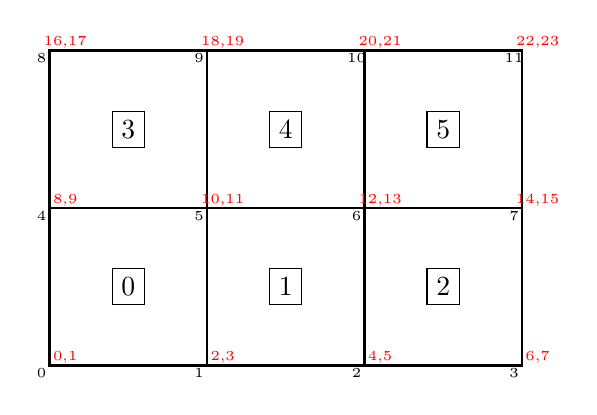
\begin{tikzpicture}
%\draw[step=0.5cm,gray,very thin] (0,0) grid (8,6); %background grid
\draw[thick] (1,1) -- (3,1) -- (3,3) -- (1,3) -- cycle;  
\draw[thick] (3,1) -- (5,1) -- (5,3) -- (3,3) -- cycle; 
\draw[thick] (5,1) -- (7,1) -- (7,3) -- (5,3) -- cycle; 
\draw[thick] (1,3) -- (3,3) -- (3,5) -- (1,5) -- cycle;  
\draw[thick] (3,3) -- (5,3) -- (5,5) -- (3,5) -- cycle; 
\draw[thick] (5,3) -- (7,3) -- (7,5) -- (5,5) -- cycle; 
\node[draw] at (2,2) {0};
\node[draw] at (4,2) {1};
\node[draw] at (6,2) {2};
\node[draw] at (2,4) {3};
\node[draw] at (4,4) {4};
\node[draw] at (6,4) {5};
%pressure dofs
\node at (0.9,0.9) {\tiny 0};
\node at (2.9,0.9) {\tiny 1};
\node at (4.9,0.9) {\tiny 2};
\node at (6.9,0.9) {\tiny 3};
\node at (0.9,2.9) {\tiny 4};
\node at (2.9,2.9) {\tiny 5};
\node at (4.9,2.9) {\tiny 6};
\node at (6.9,2.9) {\tiny 7};
\node at (0.9,4.9) {\tiny 8};
\node at (2.9,4.9) {\tiny 9};
\node at (4.9,4.9) {\tiny 10};
\node at (6.9,4.9) {\tiny 11};
%velocity dofs
\node[red] at (1.2,1.1) {\tiny 0,1};
\node[red] at (3.2,1.1) {\tiny 2,3};
\node[red] at (5.2,1.1) {\tiny 4,5};
\node[red] at (7.2,1.1) {\tiny 6,7};
\node[red] at (1.2,3.1) {\tiny 8,9};
\node[red] at (3.2,3.1) {\tiny 10,11};
\node[red] at (5.2,3.1) {\tiny 12,13};
\node[red] at (7.2,3.1) {\tiny 14,15};
\node[red] at (1.2,5.1) {\tiny 16,17};
\node[red] at (3.2,5.1) {\tiny 18,19};
\node[red] at (5.2,5.1) {\tiny 20,21};
\node[red] at (7.2,5.1) {\tiny 22,23};

\end{tikzpicture}
\end{center}

The $\K$ matrix is of size $NfemV \times NfemV$ with $NfemV=ndofV \times nnp = 2\times 12=24$.
The $\G$ matrix is of size $NfemV \times NfemP$ with $NfemP=ndofP \times nnp = 1\times 12=12$.
The $\C$ matrix is of size $NfemP \times NfemP$. 

A corner pdof sees 4 vdofs, a side pdof sees 12 vdofs and an inside pdof sees 18 vdofs, so that 
the total number of nonzeros in $\G$ can be computed as follows:
\[
NZ_\G = \underbrace{4}_{corners} + 
\underbrace{2(nnx-2)*12}_{2 hor. sides} 
+ 
\underbrace{2(nny-2)*12}_{2 vert. sides} 
+ 
\underbrace{(nnx-2)(nny-2)*18}_{inside nodes}
\]
Concretely, 
\begin{itemize}
\item pdof $\#0$ sees vdofs 0,1,2,3,8,9,10,11
\item pdof $\#1$ sees vdofs 0,1,2,3,4,5,8,9,10,11,12,13
\item pdof $\#5$ sees vdofs 0,1,2,3,4,5,8,9,10,11,12,13,16,17,18,19,20,21
\end{itemize}
so that the $\G^T$ matrix non-zero structure then is as follows:
\begin{center}
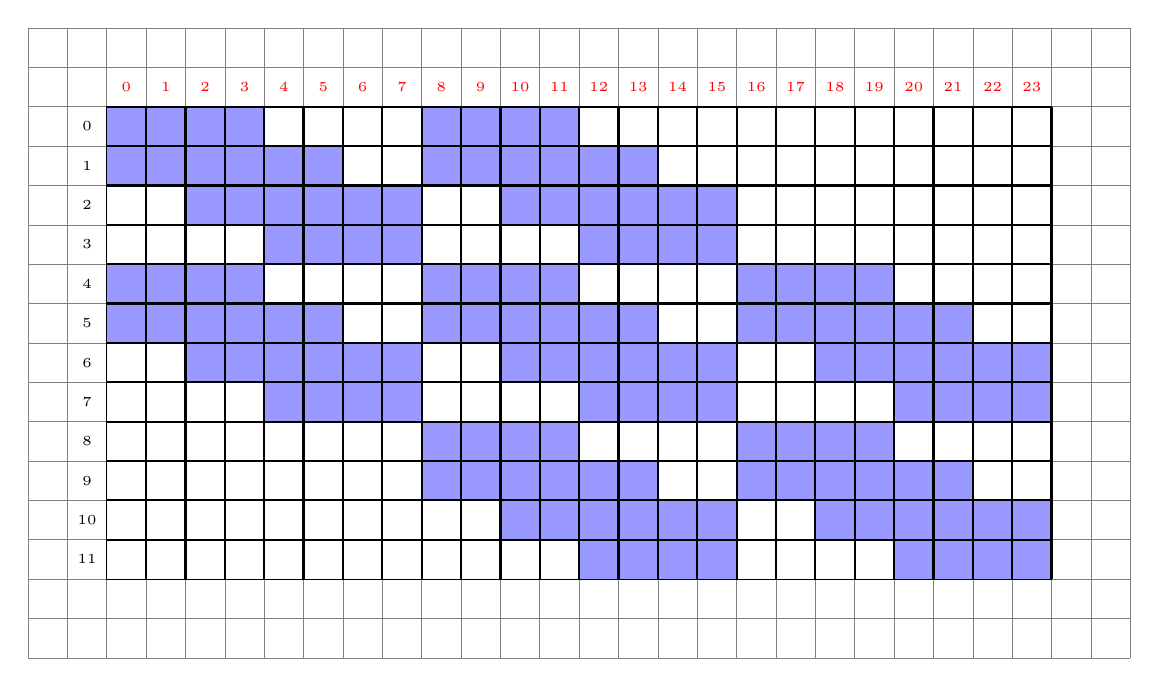
\begin{tikzpicture}
\draw[step=0.5cm,gray,very thin] (0,0) grid (14,8); %background grid
\draw (1,1) -- (13,1) -- (13,7) -- (1,7) -- cycle;    %matrix
%first top line
\fill[blue!40!white] (1.0,6.5) rectangle (1.5,7);
\fill[blue!40!white] (1.5,6.5) rectangle (2.0,7);
\fill[blue!40!white] (2.0,6.5) rectangle (2.5,7);
\fill[blue!40!white] (2.5,6.5) rectangle (3.0,7);
\fill[blue!40!white] (5.0,6.5) rectangle (5.5,7);
\fill[blue!40!white] (5.5,6.5) rectangle (6.0,7);
\fill[blue!40!white] (6.0,6.5) rectangle (6.5,7);
\fill[blue!40!white] (6.5,6.5) rectangle (7.0,7);
%second line
\fill[blue!40!white] (1.0,6.) rectangle (1.5,6.5);
\fill[blue!40!white] (1.5,6.) rectangle (2.0,6.5);
\fill[blue!40!white] (2.0,6.) rectangle (2.5,6.5);
\fill[blue!40!white] (2.5,6.) rectangle (3.0,6.5);
\fill[blue!40!white] (3.0,6.) rectangle (3.5,6.5);
\fill[blue!40!white] (3.5,6.) rectangle (4.0,6.5);
\fill[blue!40!white] (5.0,6.) rectangle (5.5,6.5);
\fill[blue!40!white] (5.5,6.) rectangle (6.0,6.5);
\fill[blue!40!white] (6.0,6.) rectangle (6.5,6.5);
\fill[blue!40!white] (6.5,6.) rectangle (7.0,6.5);
\fill[blue!40!white] (7.0,6.) rectangle (7.5,6.5);
\fill[blue!40!white] (7.5,6.) rectangle (8.0,6.5);
%third line
\fill[blue!40!white] (2.0,5.5) rectangle (2.5,6.0);
\fill[blue!40!white] (2.5,5.5) rectangle (3.0,6.0);
\fill[blue!40!white] (3.0,5.5) rectangle (3.5,6.0);
\fill[blue!40!white] (3.5,5.5) rectangle (4.0,6.0);
\fill[blue!40!white] (4.0,5.5) rectangle (4.5,6.0);
\fill[blue!40!white] (4.5,5.5) rectangle (5.0,6.0);
\fill[blue!40!white] (6.0,5.5) rectangle (6.5,6.0);
\fill[blue!40!white] (6.5,5.5) rectangle (7.0,6.0);
\fill[blue!40!white] (7.0,5.5) rectangle (7.5,6.0);
\fill[blue!40!white] (7.5,5.5) rectangle (8.0,6.0);
\fill[blue!40!white] (8.0,5.5) rectangle (8.5,6.0);
\fill[blue!40!white] (8.5,5.5) rectangle (9.0,6.0);
%fourth line
\fill[blue!40!white] (3.0,5.) rectangle (3.5,5.5);
\fill[blue!40!white] (3.5,5.) rectangle (4.0,5.5);
\fill[blue!40!white] (4.0,5.) rectangle (4.5,5.5);
\fill[blue!40!white] (4.5,5.) rectangle (5.0,5.5);
\fill[blue!40!white] (7.0,5.) rectangle (7.5,5.5);
\fill[blue!40!white] (7.5,5.) rectangle (8.0,5.5);
\fill[blue!40!white] (8.0,5.) rectangle (8.5,5.5);
\fill[blue!40!white] (8.5,5.) rectangle (9.0,5.5);
%fifth line
\fill[blue!40!white] (1.0,4.5) rectangle (1.5,5);
\fill[blue!40!white] (1.5,4.5) rectangle (2.0,5);
\fill[blue!40!white] (2.0,4.5) rectangle (2.5,5);
\fill[blue!40!white] (2.5,4.5) rectangle (3.0,5);
\fill[blue!40!white] (5.0,4.5) rectangle (5.5,5);
\fill[blue!40!white] (5.5,4.5) rectangle (6.0,5);
\fill[blue!40!white] (6.0,4.5) rectangle (6.5,5);
\fill[blue!40!white] (6.5,4.5) rectangle (7.0,5);
\fill[blue!40!white] (9.0,4.5) rectangle (9.5,5);
\fill[blue!40!white] (9.5,4.5) rectangle (10.0,5);
\fill[blue!40!white] (10.0,4.5) rectangle (10.5,5);
\fill[blue!40!white] (10.5,4.5) rectangle (11.0,5);

%sixth line
\fill[blue!40!white] (1.0,4) rectangle (1.5,4.50);
\fill[blue!40!white] (1.5,4) rectangle (2.0,4.50);
\fill[blue!40!white] (2.0,4) rectangle (2.5,4.50);
\fill[blue!40!white] (2.5,4) rectangle (3.0,4.50);
\fill[blue!40!white] (3.0,4) rectangle (3.5,4.50);
\fill[blue!40!white] (3.5,4) rectangle (4.0,4.50);


\fill[blue!40!white] (5.0,4) rectangle (5.5,4.50);
\fill[blue!40!white] (5.5,4) rectangle (6.0,4.50);
\fill[blue!40!white] (6.0,4) rectangle (6.5,4.50);
\fill[blue!40!white] (6.5,4) rectangle (7.0,4.50);
\fill[blue!40!white] (7.0,4) rectangle (7.5,4.50);
\fill[blue!40!white] (7.5,4) rectangle (8.0,4.50);

\fill[blue!40!white] (9.0,4) rectangle (9.5,4.50);
\fill[blue!40!white] (9.5,4) rectangle (10.0,4.50);
\fill[blue!40!white] (10.0,4) rectangle (10.5,4.50);
\fill[blue!40!white] (10.5,4) rectangle (11.0,4.50);
\fill[blue!40!white] (11.0,4) rectangle (11.5,4.50);
\fill[blue!40!white] (11.5,4) rectangle (12.0,4.50);




%seventh line
\fill[blue!40!white] (2.0,3.5) rectangle (2.5,4.0);
\fill[blue!40!white] (2.5,3.5) rectangle (3.0,4.0);
\fill[blue!40!white] (3.0,3.5) rectangle (3.5,4.0);
\fill[blue!40!white] (3.5,3.5) rectangle (4.0,4.0);
\fill[blue!40!white] (4.0,3.5) rectangle (4.5,4.0);
\fill[blue!40!white] (4.5,3.5) rectangle (5.0,4.0);
\fill[blue!40!white] (6.0,3.5) rectangle (6.5,4.0);
\fill[blue!40!white] (6.5,3.5) rectangle (7.0,4.0);
\fill[blue!40!white] (7.0,3.5) rectangle (7.5,4.0);
\fill[blue!40!white] (7.5,3.5) rectangle (8.0,4.0);
\fill[blue!40!white] (8.0,3.5) rectangle (8.5,4.0);
\fill[blue!40!white] (8.5,3.5) rectangle (9.0,4.0);
\fill[blue!40!white] (10.0,3.5) rectangle (10.5,4.0);
\fill[blue!40!white] (10.5,3.5) rectangle (11.0,4.0);
\fill[blue!40!white] (11.0,3.5) rectangle (11.5,4.0);
\fill[blue!40!white] (11.5,3.5) rectangle (12.0,4.0);
\fill[blue!40!white] (12.0,3.5) rectangle (12.5,4.0);
\fill[blue!40!white] (12.5,3.5) rectangle (13.0,4.0);
%eighth line
\fill[blue!40!white] (3.0,3.) rectangle (3.5,3.5);
\fill[blue!40!white] (3.5,3.) rectangle (4.0,3.5);
\fill[blue!40!white] (4.0,3.) rectangle (4.5,3.5);
\fill[blue!40!white] (4.5,3.) rectangle (5.0,3.5);
\fill[blue!40!white] (7.0,3.) rectangle (7.5,3.5);
\fill[blue!40!white] (7.5,3.) rectangle (8.0,3.5);
\fill[blue!40!white] (8.0,3.) rectangle (8.5,3.5);
\fill[blue!40!white] (8.5,3.) rectangle (9.0,3.5);
\fill[blue!40!white] (11.0,3.) rectangle (11.5,3.5);
\fill[blue!40!white] (11.5,3.) rectangle (12.0,3.5);
\fill[blue!40!white] (12.0,3.) rectangle (12.5,3.5);
\fill[blue!40!white] (12.5,3.) rectangle (13.0,3.5);
%9th line
\fill[blue!40!white] (5.0,2.5) rectangle (5.5,3);
\fill[blue!40!white] (5.5,2.5) rectangle (6.0,3);
\fill[blue!40!white] (6.0,2.5) rectangle (6.5,3);
\fill[blue!40!white] (6.5,2.5) rectangle (7.0,3);
\fill[blue!40!white] (9.0,2.5) rectangle (9.5,3);
\fill[blue!40!white] (9.5,2.5) rectangle (10.0,3);
\fill[blue!40!white] (10.0,2.5) rectangle (10.5,3);
\fill[blue!40!white] (10.5,2.5) rectangle (11.0,3);
%10th line
\fill[blue!40!white] (5.0,2) rectangle (5.5,2.5);
\fill[blue!40!white] (5.5,2) rectangle (6.0,2.5);
\fill[blue!40!white] (6.0,2) rectangle (6.5,2.5);
\fill[blue!40!white] (6.5,2) rectangle (7.0,2.5);
\fill[blue!40!white] (7.0,2) rectangle (7.5,2.5);
\fill[blue!40!white] (7.5,2) rectangle (8.0,2.5);
\fill[blue!40!white] (9.0,2) rectangle (9.5,2.5);
\fill[blue!40!white] (9.5,2) rectangle (10.0,2.5);
\fill[blue!40!white] (10.0,2) rectangle (10.5,2.5);
\fill[blue!40!white] (10.5,2) rectangle (11.0,2.5);
\fill[blue!40!white] (11.0,2) rectangle (11.5,2.5);
\fill[blue!40!white] (11.5,2) rectangle (12.0,2.5);
%11th line
\fill[blue!40!white] (6.0,1.5) rectangle (6.5,2);
\fill[blue!40!white] (6.5,1.5) rectangle (8,2);
\fill[blue!40!white] (7.0,1.5) rectangle (7.5,2);
\fill[blue!40!white] (7.5,1.5) rectangle (8.0,2);
\fill[blue!40!white] (8.0,1.5) rectangle (8.5,2);
\fill[blue!40!white] (8.5,1.5) rectangle (9.0,2);
\fill[blue!40!white] (10.0,1.5) rectangle (10.5,2);
\fill[blue!40!white] (10.5,1.5) rectangle (11.0,2);
\fill[blue!40!white] (11.0,1.5) rectangle (11.5,2);
\fill[blue!40!white] (11.5,1.5) rectangle (12.0,2);
\fill[blue!40!white] (12.0,1.5) rectangle (12.5,2);
\fill[blue!40!white] (12.5,1.5) rectangle (13.0,2);
%12th line
\fill[blue!40!white] (7.0,1.0) rectangle (7.5,1.5);
\fill[blue!40!white] (7.5,1.0) rectangle (8.0,1.5);
\fill[blue!40!white] (8.0,1.0) rectangle (8.5,1.5);
\fill[blue!40!white] (8.5,1.0) rectangle (9.0,1.5);
\fill[blue!40!white] (11.0,1.0) rectangle (11.5,1.5);
\fill[blue!40!white] (11.5,1.0) rectangle (12.0,1.5);
\fill[blue!40!white] (12.0,1.0) rectangle (12.5,1.5);
\fill[blue!40!white] (12.5,1.0) rectangle (13.0,1.5);
%vertical
\node at (0.75,6.75) {\tiny 0};
\node at (0.75,6.25) {\tiny 1};
\node at (0.75,5.75) {\tiny 2};
\node at (0.75,5.25) {\tiny 3};
\node at (0.75,4.75) {\tiny 4};
\node at (0.75,4.25) {\tiny 5};
\node at (0.75,3.75) {\tiny 6};
\node at (0.75,3.25) {\tiny 7};
\node at (0.75,2.75) {\tiny 8};
\node at (0.75,2.25) {\tiny 9};
\node at (0.75,1.75) {\tiny 10};
\node at (0.75,1.25) {\tiny 11};
%horizontal
\node[red] at (1.25,7.25) {\tiny 0};
\node[red] at (1.75,7.25) {\tiny 1};
\node[red] at (2.25,7.25) {\tiny 2};
\node[red] at (2.75,7.25) {\tiny 3};
\node[red] at (3.25,7.25) {\tiny 4};
\node[red] at (3.75,7.25) {\tiny 5};
\node[red] at (4.25,7.25) {\tiny 6};
\node[red] at (4.75,7.25) {\tiny 7};
\node[red] at (5.25,7.25) {\tiny 8};
\node[red] at (5.75,7.25) {\tiny 9};
\node[red] at (6.25,7.25) {\tiny 10};
\node[red] at (6.75,7.25) {\tiny 11};
\node[red] at (7.25,7.25) {\tiny 12};
\node[red] at (7.75,7.25) {\tiny 13};
\node[red] at (8.25,7.25) {\tiny 14};
\node[red] at (8.75,7.25) {\tiny 15};
\node[red] at (9.25,7.25) {\tiny 16};
\node[red] at (9.75,7.25) {\tiny 17};
\node[red] at (10.25,7.25) {\tiny 18};
\node[red] at (10.75,7.25) {\tiny 19};
\node[red] at (11.25,7.25) {\tiny 20};
\node[red] at (11.75,7.25) {\tiny 21};
\node[red] at (12.25,7.25) {\tiny 22};
\node[red] at (12.75,7.25) {\tiny 23};
\draw[step=0.5cm,black,thick] (1,1) grid (13,7); %background grid
\end{tikzpicture}
\end{center}

\noindent
\underline{Non-zero pattern of the $\C$ matrix}: Let us take a simple example: a 3x2 element grid.

\todo[inline]{finish structure of C matrix for q1q1}







We impose $\int p dV=0$ which means that the following constraint is added 
to the Stokes matrix:
\[
\left(
\begin{array}{ccc}
\K & \G & 0\\ 
\G^T & \C & \LLL \\
0 & \LLL^T & 0 
\end{array}
\right)
\cdot
\left(
\begin{array}{c}
{\cal V} \\ {\cal P} \\ \lambda
\end{array}
\right)
=
\left(
\begin{array}{c}
 f \\ h \\ 0
\end{array}
\right)
\]











%-----------------------------------------
\subsection{The Donea \& Huerta benchmark}

As in \cite{dohu03} we solve the benchmark problem presented in section \ref{mms1}.

\includegraphics[width=10cm]{python_codes/fieldstone_22/results/case1/errors.pdf}

%-----------------------------------------
\subsection{The Dohrmann \& Bochev benchmark} 

As in \cite{dobo04} we solve the benchmark problem presented in section \ref{mms2}.

\includegraphics[width=10cm]{python_codes/fieldstone_22/results/case2/errors.pdf}

\todo[inline]{compare my rates with original paper!}

%\includegraphics[width=5cm]{python_codes/fieldstone_22/results/uth}
%\includegraphics[width=5cm]{python_codes/fieldstone_22/results/vth}
%\includegraphics[width=5cm]{python_codes/fieldstone_22/results/pth}

%-----------------------------------------
\subsection{The falling block experiment} 

The setup is desscribed in \cite{thba19}.

\includegraphics[width=10cm]{python_codes/fieldstone_22/results/case3/fallingblock.pdf}








\newpage
%%%%%%%%%%%%%%%%%%%%%%%%%%%%%%%%%%%%%%%%%%%%%%%%%%%%%%%%%%%%%%%%%%%%%%%%%%%%%%%
\section{{\tt fieldstone\_23}: compressible flow (1) - analytical benchmark \label{f23}}
\lstinputlisting[language=bash,basicstyle=\small]{python_codes/fieldstone_23/keywords.ascii}

\begin{center}
Code at \url{https://github.com/cedrict/fieldstone/tree/master/python_codes/fieldstone_23}
\end{center}

\par\noindent\rule{\textwidth}{0.4pt}

This work is part of the MSc thesis of T. Weir (2018).
\index{contributors}{T. Weir}

\par\noindent\rule{\textwidth}{0.4pt}
%%%%%%%%%%%%%%%%%%%%%%%%%%%%%%%%%%%%%%%%%%%%%%%%%%%%%%%%%%%%%%%%%%%%%%%%%%%%%%%%%%

We first start with an isothermal Stokes flow, so that we disregard the heat transport equation and 
the equations we wish to solve are simply:

\begin{align}
  -\nabla \cdot \left[2\eta \left(\dot\varepsilon(\bm v)
                                  - \frac{1}{3}(\nabla \cdot \bm v)\mathbf 1\right)
                \right] + \nabla p &=
  \rho \bm g
  &
  & \textrm{in $\Omega$},
  \\
  \nabla \cdot (\rho \bm v) &= 0
  &
  & \textrm{in $\Omega$}
\end{align}
The second equation can be rewritten 
$\nabla \cdot (\rho {\bm v}) =  \rho \nabla \cdot {\bm v} + {\bm v} \cdot {\bm \nabla}\rho=0$
or, 
\[
\nabla \cdot {\bm v} + \frac{1}{\rho} {\bm v} \cdot {\bm \nabla}\rho=0
\]
Note that this presupposes that the density is not zero anywhere in the domain.

We use a mixed formulation and therefore  
keep both velocity and pressure as unknowns. We end up having to solve 
the following system:
\[
\left(
\begin{array}{cc}
\K & \G \\ \G^T+\Z & 0 
\end{array}
\right)
\cdot
\left(
\begin{array}{c}
{\cal V} \\ {\cal P}
\end{array}
\right)
=
\left(
\begin{array}{c}
 f \\ h
\end{array}
\right)
\quad\quad
{\rm or,}
\quad\quad
\A \cdot X = rhs
\]
Where $\K$ is the stiffness matrix, $\G$ is the discrete gradient operator, 
$\G^T$ is the discrete divergence operator, ${\cal V}$ the velocity vector, 
${\cal P}$ the pressure vector.
Note that the term $\Z{\cal V}$ derives from term ${\bm v} \cdot {\bm \nabla} \rho$ in the continuity equation. 

Each block $\K$, $\G$ , $\Z$ and vectors $f$ and $h$ are built separately 
in the code and assembled into 
the matrix $\A$ and vector $rhs$ afterwards. $\A$ and $rhs$ are then passed to the solver. 
We will see later that there are alternatives to solve this approach which do not require to 
build the full Stokes matrix $\A$. 

{\sl Remark}: the term $\Z {\cal V}$ is often put in the rhs (i.e. added to $h$) so that 
the matrix $\A$ retains the same structure as in the incompressible case. This is indeed 
how it is implemented in ASPECT. This however requires more work since the rhs depends 
on the solution and some form of iterations is needed. 

In the case of a compressible flow the strain rate tensor and the deviatoric strain rate tensor are no more equal (since ${\bm \nabla}\cdot{\bm v} \neq 0$).
The deviatoric strainrate tensor is given by\footnote{See the ASPECT manual for a justification of the 3 value in the denominator in 2D and 3D.} 
\[
\dot{\bm \epsilon}^d({\bm v})=
\dot{\bm \epsilon}({\bm v})-\frac{1}{3} Tr(\dot{\bm \epsilon}) {\bm 1}
=\dot{\bm \epsilon}({\bm v})-\frac{1}{3} ({\bm \nabla}\cdot{\bm v}) {\bm 1}
\]
In that case:
\begin{eqnarray}
\dot{\epsilon}_{xx}^d 
&=& \frac{\partial u}{\partial x}
-\frac{1}{3} \left( \frac{\partial u}{\partial x} + \frac{\partial v}{\partial y} \right) 
= \frac{2}{3}\frac{\partial u}{\partial x}
-\frac{1}{3} \frac{\partial v}{\partial y}
%=
%\frac{2}{3} \sum_{i=1}^4 \frac{\partial N_i}{\partial x}\;  u_i 
%-\frac{1}{3} \sum_{i=1}^4 \frac{\partial N_i}{\partial y}\;  v_i 
\\
\dot{\epsilon}_{yy}^d 
&=& \frac{\partial v}{\partial y}
-\frac{1}{3} \left( \frac{\partial u}{\partial x} + \frac{\partial v}{\partial y} \right) 
=-\frac{1}{3} \frac{\partial u}{\partial x} 
+ \frac{2}{3} \frac{\partial v}{\partial y} 
%=-\frac{1}{3}  \sum_{i=1}^4 \frac{\partial N_i}{\partial x}\;  u_i
%+ \frac{2}{3} \sum_{i=1}^4 \frac{\partial N_i}{\partial y}\;  v_i
\\
2\dot{\epsilon}_{xy}^d 
&=& 
\frac{\partial u}{\partial y} 
+\frac{\partial v}{\partial x} 
%= \sum_{i=1}^4 \frac{\partial N_i}{\partial y}\;  u_i
%+ \sum_{i=1}^4 \frac{\partial N_i}{\partial x}\;  v_i
\end{eqnarray}
and then 
\[
\dot{\bm \epsilon}^d({\bm v})
=
\left(
\begin{array}{cc}
\frac{2}{3} \frac{\partial u}{\partial x} -\frac{1}{3} \frac{\partial v}{\partial y} &
\frac{1}{2}\frac{\partial u}{\partial y} + \frac{1}{2}\frac{\partial v}{\partial x}  \\ \\
\frac{1}{2}\frac{\partial u}{\partial y} + \frac{1}{2}\frac{\partial v}{\partial x}  &
-\frac{1}{3} \frac{\partial u}{\partial x} +\frac{2}{3} \frac{\partial v}{\partial y} 
\end{array}
\right)
\]

From $\vec{\tau} = 2\eta \vec{\epsilon}^d$ we arrive at:
\[
\left(
\begin{array}{c}
\tau_{xx}\\
\tau_{yy}\\
\tau_{xy}\\
\end{array}
\right)
=
2\eta
\left(
\begin{array}{c}
\dot{\epsilon}_{xx}^d \\
\dot{\epsilon}_{yy}^d \\
\dot{\epsilon}_{xy}^d 
\end{array}
\right)
=2 \eta
\left(
\begin{array}{ccc}
2/3 & -1/3& 0 \\
-1/3 & 2/3 & 0 \\
0 & 0 & 1/2 \\
\end{array}
\right)
\cdot 
\left(
\begin{array}{c}
\frac{\partial u}{\partial x} \\ 
\frac{\partial v}{\partial y} \\ 
\frac{\partial u}{\partial y}\! +\! \frac{\partial v}{\partial x} \\
\end{array}
\right)
=
\eta
\left(
\begin{array}{ccc}
4/3 & -2/3& 0 \\
-2/3 & 4/3 & 0 \\
0 & 0 & 1 \\
\end{array}
\right)
\cdot 
\left(
\begin{array}{c}
\frac{\partial u}{\partial x} \\ 
\frac{\partial v}{\partial y} \\ 
\frac{\partial u}{\partial y}\! +\! \frac{\partial v}{\partial x} \\
\end{array}
\right)
\]
or, 
\[
\vec{\tau} = {\bm C}_\eta {\bm B} V
\]


















\newpage
In order to test our implementation we have created a few manufactured solutions:
\begin{itemize}
\item \underline{benchmark \#1} ({\tt ibench=1})): Starting from a density profile of:
\begin{equation}
    \rho(x,y) = xy
\end{equation}
We derive a velocity given by:
\begin{equation}
    v_x(x,y) = \frac{C_x}{x} , v_y(x,y) = \frac{C_y}{y}
\end{equation}

With $g_x(x,y) = \frac{1}{x}$ and $g_y(x,y) = \frac{1}{y}$, this leads us to a pressure profile:
\begin{equation}
    p = - \eta \left( \frac{4C_x}{3x^2} + \frac{4C_y}{3y^2} \right)  + xy + C_0
\end{equation}
This gives us a strain rate:
\[
\dot{\epsilon}_{xx} =  \frac{-C_x}{x^2}
\quad
\quad
\quad
\dot{\epsilon}_{yy} =  \frac{-C_y}{y^2}
\quad
\quad
\quad
\dot{\epsilon}_{xy} = 0 
\]
In what follows, we choose $\eta=1$ and $C_x=C_y=1$ and for a unit square domain $
[1:2]\times[1:2]$ we compute $C_0$
so that the pressure is normalised to zero over the whole domain and obtain $C_0=-1$. 
 
\item \underline{benchmark \#2} ({\tt ibench=2}): Starting from a density profile of:
\begin{equation}
    \rho = \cos(x)\cos(y)
\end{equation}
We derive a velocity given by:
\begin{equation}
    v_x = \frac{C_x}{\cos(x)} , v_y = \frac{C_y}{\cos(y)}
\end{equation}
With $g_x = \frac{1}{\cos(y)}$ and $g_y = \frac{1}{\cos(x)}$, this leads us to a pressure profile:
\begin{equation}
    p =  \eta \Bigg(\frac{4C_x \sin(x)}{3\cos^2(x)} + \frac{4C_y \sin(y)}{3\cos^2(y)}\Bigg) 
    +( \sin(x) + \sin(y) ) + C_0
\end{equation}
\[
\dot{\epsilon}_{xx} = C_x \frac{\sin(x)}{\cos^2(x)}
\quad
\quad
\quad
\dot{\epsilon}_{yy} = C_y \frac{\sin(y)}{\cos^2(y)}
\quad
\quad
\quad
\dot{\epsilon}_{xy} = 0 
\]
We choose $\eta=1$ and $C_x=C_y=1$. The domain is the unit square $[0:1]\times[0:1]$ and we obtain 
$C_0$ as before and obtain 
\[
C_0 = 2 - 2 \cos(1) + 8/3 (\frac{1}{\cos (1)} - 1)
\simeq 3.18823730
\]
(thank you WolframAlpha)


\item \underline{benchmark \#3} ({\tt ibench=3}) 
\item \underline{benchmark \#4} ({\tt ibench=4}) 
\item \underline{benchmark \#5} ({\tt ibench=5}) 
\end{itemize}





%\includegraphics[width=16cm]{python_codes/fieldstone_saddlepoint/solution.pdf}

ToDo:
\begin{itemize}
\item pbs with odd vs even number of elements 
\item q is 'fine' everywhere except in the corners - revisit pressure smoothing paper?
\item redo A v d Berg benchmark (see Tom Weir thesis)
\end{itemize}




\newpage
%%%%%%%%%%%%%%%%%%%%%%%%%%%%%%%%%%%%%%%%%%%%%%%%%%%%%%%%%%%%%%%%%%%%%%%%%%%%%%%
\section{{\tt fieldstone\_24}: compressible flow (2) - convection box \label{f24}}

\index{stones}{$Q_1 \times P_0$ element}
\index{stones}{Compressible Flow}
\index{stones}{Mixed Formulation}
\index{stones}{Analytical Solution}
\index{stones}{Pressure Smoothing} 


\begin{mdframed}[backgroundcolor=red!5]
This work is part of the MSc thesis of T. Weir (2018).
\end{mdframed}
\index{contributors}{T. Weir}

\Literature \cite{itki94,tagu07,lezh08,kilv10,lezh11,lizh13,hedg17,civj17}

\subsection*{The physics}

Let us start with some thermodynamics. Every material has an equation of state.
The equilibrium thermodynamic state of any material can
be constrained if any two state variables are specified.
Examples of state variables include
the pressure $p$ and specific volume $\nu = 1/\rho$, as well as the temperature $T$.

After linearisation, the density depends on temperature and pressure as follows:
\[
\rho(T,p) = \rho_0 \left((1 - \alpha(T-T_0) + \beta_T p \right)
\]
where $\alpha$ is the coefficient of thermal expansion, also called 
thermal expansivity: \index{stones}{thermal expansion}
\[
\alpha=-\frac{1}{\rho}\left( \frac{\partial \rho}{\partial T} \right)_p
\]
$\alpha$ is the percentage increase in volume of a material per degree of temperature increase; the
subscript $p$ means that the pressure is held fixed.

$\beta_T$ is the isothermal compressibility of the fluid, which is given by \index{stones}{compressibility}
\[
\beta_T = \frac{1}{K} = \frac{1}{\rho}\left( \frac{\partial \rho}{\partial P} \right)_T
\]
with $K$ the bulk modulus. \index{stones}{bulk modulus}
%aspect manual
Values of $\beta_T=10^{-12}-10^{-11}$ Pa$^{-1}$ are reasonable for Earth's mantle, with values decreasing by about a
factor of 5 between the shallow lithosphere and core-mantle boundary.
This is the percentage increase in density per unit change in pressure at constant temperature.
Both the coefficient of thermal expansion and the isothermal compressibility can be obtained
from the equation of state.

The full set of equations we wish to solve is given by

\begin{eqnarray}
-\nabla \cdot \left[2\eta \dot{\bm \epsilon}^d({\bm v}) \right] + \nabla p &=& \rho_0 \left((1 - \alpha(T-T_0) + \beta_T p \right) {\bm g} \quad\quad \textrm{in $\Omega$}  \label{eq:stokes-1} \\
\nabla \cdot {\bm v} + \frac{1}{\rho} {\bm v} \cdot {\bm \nabla}\rho&=&0 \quad\quad  \textrm{in $\Omega$}   \label{eq:stokes-2} \\
\rho C_p \left(\frac{\partial T}{\partial t} + \bm v\cdot\nabla T\right) - \nabla\cdot k\nabla T   &=& 
  \rho H  +  2\eta \dot{\bm \epsilon}^d : \dot{\bm \epsilon}^d    +\alpha T \left( \frac{\partial p}{\partial t}+  \bm v \cdot \nabla p \right) 
\quad\quad   \textrm{in $\Omega$},
  \label{eq:temperature}
\end{eqnarray}

Note that this presupposes that the density is not zero anywhere in the domain.


\subsection*{The numerics}

We use a mixed formulation and therefore  
keep both velocity and pressure as unknowns. We end up having to solve 
the following system:
\[
\left(
\begin{array}{cc}
\K & \G+\W \\ \G^T+\Z & 0 
\end{array}
\right)
\cdot
\left(
\begin{array}{c}
{\cal V} \\ {\cal P}
\end{array}
\right)
=
\left(
\begin{array}{c}
 f \\ h
\end{array}
\right)
\quad\quad
{\rm or,}
\quad\quad
\A \cdot X = rhs
\]
Where $\K$ is the stiffness matrix, $\G$ is the discrete gradient operator, 
$\G^T$ is the discrete divergence operator, ${\cal V}$ the velocity vector, 
${\cal P}$ the pressure vector.
Note that the term $\Z{\cal V}$ derives from term ${\bm v} \cdot {\bm \nabla} \rho$ in the continuity equation. 

As perfectly explained in the step 32 of deal.ii\footnote{https://www.dealii.org/9.0.0/doxygen/deal.II/step\_32.html},
we need to scale the $\G$ term since it is many orders of magnitude smaller than $\K$, which introduces large inaccuracies in the solving process to the point that the solution is nonsensical. This scaling coefficient is $\eta/L$. After building the $\G$ block, it is then scaled as follows: $\G'=\frac{\eta}{L}\G$ so that we now solve 

\[
\left(
\begin{array}{cc}
\K & \G'+\W \\ \G'^T+\Z & 0 
\end{array}
\right)
\cdot
\left(
\begin{array}{c}
{\cal V} \\ {\cal P}'
\end{array}
\right)
=
\left(
\begin{array}{c}
 f \\ h
\end{array}
\right)
\]
After the solve phase, we recover the real pressure with ${\cal P}=\frac{\eta}{L}{\cal P}'$.

{\color{red} adapt notes since I should scale $\W$ and $\Z$ too}.
{\color{red} $h$ should be caled too !!!!!!!!!!!!!!!} 

Each block $\K$, $\G$ , $\Z$ and vectors $f$ and $h$ are built separately 
in the code and assembled into 
the matrix $\A$ and vector $rhs$ afterwards. $\A$ and $rhs$ are then passed to the solver. 
We will see later that there are alternatives to solve this approach which do not require to 
build the full Stokes matrix $\A$. 

{\bf Remark 1}: the terms $\Z {\cal V}$ and $\W {\cal P}$ are 
often put in the rhs (i.e. added to $h$) so that 
the matrix $\A$ retains the same structure as in the incompressible case. This is indeed 
how it is implemented in ASPECT, see also appendix A of \cite{lezh08}. This however requires more work since the rhs depends 
on the solution and some form of iterations is needed. 

{\bf Remark 2}: Very often the adiabatic heating term  
$\alpha T \left( \bm v \cdot \nabla p \right)$ is simplified as follows:
%aspect manual
If you assume the vertical component of the gradient of the dynamic pressure to be small compared to the
gradient of the total pressure (in other words, the gradient is dominated by the gradient of the hydrostatic
pressure), then $-\rho {\bm g} \simeq {\bm \nabla}p$ and then 
$\alpha T \left( \bm v \cdot \nabla p \right) \simeq  -\alpha\rho T {\bm v}\cdot{\bm g}$. We will however 
not be using this approximation in what follows.



We have already established that
\[
\vec{\tau} = {\bm C}_\eta {\bm B} V
\]


The following measurements are carried out:
\begin{itemize}
\item The root mean square velocity ({\tt vrms}):
\[
v_{rms} = \sqrt{\frac{1}{V}\int_V v^2 dV   }
\]
\item The average temperature ({\tt Tavrg}):
\[
<T>=\frac{1}{V}\int_V T dV
\]
\item The total mass ({\tt mass}):
\[
M=\int_V \rho dV 
\]
\item The Nusselt number ({\tt Nu}):
\[
Nu=-\frac{1}{Lx}\frac{1}{\Delta T} \int_0^{L_x} \frac{\partial T(x,y=L_y)}{\partial y} dx
\]
\item The kinetic energy ({\tt EK}):
\[
E_K=\int_V \frac{1}{2}\rho v^2 dV
\]
\item The work done against gravity 
\[
<W>=-\int_V \rho g_y v_y dV
\]
\item The total viscous dissipation ({\tt visc\_diss})
\[
<\Phi>=\int \Phi dV =\frac{1}{V}\int 2 \eta \dot{\bm \varepsilon}:\dot{\bm \varepsilon} dV 
\]
\item The gravitational potential energy ({\tt EG})
\[
E_G = \int_V \rho g_y (L_y-y) dV
\]
\item The internal thermal energy ({\tt ET})
\[
E_T = \int_V \rho_{(0)} C_p T dV
\]

{\bf Remark 3:} Measuring the total mass can be misleading: indeed because $\rho=\rho_0(1-\alpha T)$, then 
measuring the total mass amounts to measuring a constant minus the volume-integrated temperature, and there is 
no reason why the latter should be zero, so that there is no reason why the total mass should be zero...!

\end{itemize}




\subsection*{The experimental setup}

The setup is as follows: the domain is $Lx=Ly=3000$km. Free slip boundary conditions are imposed on all four sides. 
The initial temperature is given by:
\[
T(x,y) = \left(  \frac{L_y-y}{Ly} - 0.01\cos(\frac{\pi x}{L_x}) \sin(\frac{\pi y}{Ly}) \right) \Delta T + T_{surf}
\]
with $\Delta T=4000$K, $T_{surf}=T_0=273.15$K. The temperature is set to $\Delta T + T_{surf}$ at the bottom and $T_{surf}$ at the top.
We also set $k=3$, $C_p=1250$, $|g|=10$, $\rho_0=3000$ and we keep the Rayleigh number $Ra$ and dissipation number $Di$ as input parameters:
\[
Ra=\frac{\alpha g \Delta T L^3 \rho_0^2 C_p}{\eta k}
\quad\quad
Di=\frac{\alpha g L}{C_p}
\]
From the second equation we get $\alpha=\frac{Di C_p}{g L}$, which we can insert in the first one:
\[
Ra=\frac{Di C_p^2 \Delta T L^2 \rho_0^2 }{\eta k}
\quad\quad
{\rm or,}
\quad\quad
\eta=
\frac{Di C_p^2 \Delta T L^2 \rho_0^2 }{Ra \; k  }
\]
For instance, for $Ra=10^4$ and $Di=0.75$, we obtain $\alpha\simeq 3\cdot 10^{-5}$ and $\eta\simeq 10^{25}$ 
which are quite reasonable values. 


\subsection*{Scaling}

Following \cite{kilv10}, we non-dimensionalize the equations using the reference values
for density $\rho_r$, thermal expansivity $\alpha_r$, 
temperature contrast $\Delta T_r$ ({\tt refTemp}),
thermal conductivity $k_r$, heat capacity $C_p$,  
depth of the fluid layer $L$ and viscosity $\eta_r$. The
non-dimensionalization for velocity, $u_r$ , pressure $p_r$ and time, $t_r$ become
\[
u_r = \frac{k_r}{\rho_r C_p L} \quad ({\tt refvel})
\]
\[
p_r=\frac{\eta_r k_r}{\rho_r C_p L^2}\quad  ({\tt refpress})
\]
\[
t_r=\frac{\rho_r C_p L^2}{k_r} \quad ({\tt reftime})
\]

In the case of the setup described hereabove, and when choosing 
$Ra=10^4$ and $Di=0.5$, we get:
\begin{verbatim}
alphaT 2.083333e-05 
eta 8.437500e+24 
reftime 1.125000e+19 
refvel 2.666667e-13 
refPress 7.500000e+05 
\end{verbatim}



%-------------------------------------------
\subsection*{Conservation of energy 1}



\subsubsection*{under BA and EBA approximations}

Following \cite{lezh08}, we take the dot product of the momentum equation with the velocity ${\bm v}$ and integrate over the whole volume\footnote{Check: this is akin to looking at the power, force*velocity,  says Arie}:
\[
\int_V  \left[ -\nabla \cdot {\bm \tau}  + {\bm \nabla} p \right] \cdot {\bm v} dV  = \int_V  \rho {\bm g} \cdot {\bm v}dV
\]
or, 
\[
-\int_V (\nabla \cdot {\bm \tau})\cdot {\bm v} dV +\int_V   {\bm \nabla} p \cdot {\bm v} dV  = \int_V  \rho {\bm g} \cdot {\bm v}dV
\]
Let us look at each block separately:
\[
-\int_V (\nabla \cdot {\bm \tau})\cdot {\bm v} dV 
=-\int_S  {\bm \tau} \underbrace{{\bm v}\cdot {\bm n}}_{=0 \; (b.c.)} dS + \int_V {\bm \tau}:{\bm \nabla}{\bm v} dV 
= \int_V {\bm \tau} : \dot{\bm \varepsilon} dV 
= \int_V \Phi  dV 
\]
which is the volume integral of the shear heating. Then,
\[
\int_V {\bm \nabla} p \cdot {\bm v} dV  =
\int_S p \underbrace{{\bm v}\cdot {\bm n}}_{=0 \; (b.c.)} dS - \int_V \underbrace{{\bm \nabla}\cdot{\bm v}}_{=0 \; (incomp.)} \; p dV = 0 
\]
which is then zero in the case of an incompressible flow. 
And finally
\[
\int_V \rho {\bm g} \cdot {\bm v} dV = W
\]
which is the work against gravity. \index{stones}{work against gravity} 

Conclusion for an {\it incompressible} fluid: we should have
\begin{equation}
\int_V \Phi  dV 
=
\int_V \rho {\bm g} \cdot {\bm v} dV 
\label{ba001}
\end{equation}
This formula is hugely problematic: indeed, the term $\rho$ in the rhs is the full density. We know 
that to the value of $\rho_0$ corresponds a lithostatic pressure gradient $p_L=\rho_0 g y$. In this case one can write $\rho = \rho_0 + \rho'$ and $p=p_L + p'$
so that we also have 
\[
\int_V  \left[ -\nabla \cdot {\bm \tau}  + {\bm \nabla} p' \right] \cdot {\bm v} dV  = \int_V  \rho' {\bm g} \cdot {\bm v}dV
\]
which will ultimately yield 
\begin{equation}
\int_V \Phi  dV 
=
\int_V \rho' {\bm g} \cdot {\bm v} dV 
=
\int_V (\rho-\rho_0) {\bm g} \cdot {\bm v} dV 
\label{ba002}
\end{equation}
Obviously Eqs.(\ref{ba001}) and (\ref{ba002}) cannot be true at the same time.
The problem comes from the nature of the (E)BA approximation: $\rho=\rho_0$ in the mass conservation equation
but it is not constant in the momentum conservation equation, which is of course inconsistent. Since the mass 
conservation equation is ${\bm \nabla}\cdot{\bm v}=0$ under this approximation then the term 
$\int_V {\bm \nabla} p \cdot {\bm v} dV$ is always zero for any pressure (full pressure $p$, or overpressure $p-p_L$), 
hence the paradox. This paradox will be lifted when a consistent set of equations will be used (compressible formulation).
On a practical note, Eqs.(\ref{ba001}) is not verified by the code, while (\ref{ba002}) is.   

In the end:
\begin{equation}
\boxed{
\underbrace{\int_V \Phi  dV }_{\tt visc\_diss}
=
\underbrace{\int_V (\rho-\rho_0) {\bm g} \cdot {\bm v} dV }_{\tt work\_grav}
}
\label{ba003}
\end{equation}


\subsubsection*{under no  approximation at all}

\begin{eqnarray}
\int_V {\bm \nabla} p \cdot {\bm v} dV  
&=& \int_S p \underbrace{{\bm v}\cdot {\bm n}}_{=0 \; (b.c.)} dS - \int_V {\bm \nabla}\cdot{\bm v} \; p dV = 0  \\
&=&  \int_V \frac{1}{\rho} {\bm v} \cdot {\bm \nabla} \rho \; p dV = 0  \\
\end{eqnarray}

{\color{red} ToDo}:see section 3 of \cite{lezh08} where this is carried out with the Adams-Williamson eos.


\subsection*{Conservation of energy 2}
Also, following the Reynold's transport theorem \cite{malvern},p210, we have for a property $A$ (per unit mass)
\[
\frac{d}{dt} \int_V A \rho dV = \int_V \frac{\partial }{\partial t} (A\rho) dV + \int_S A \rho {\bm v}\cdot {\bm n} dS
\]
Let us apply to this to $A=C_p T$ and compute the time derivative of the internal energy:
\begin{eqnarray}
\frac{d}{dt} \int_V \rho C_p T dV 
&=& \int_V \frac{\partial }{\partial t} (\rho C_p T ) dV + \int_S A \rho \underbrace{{\bm v}\cdot {\bm n}}_{=0 \; (b.c.)} dS 
= \underbrace{\int_V C_p T \frac{\partial \rho}{\partial t} dV}_{I} 
+ \underbrace{\int_V \rho C_p \frac{\partial T}{\partial t}  dV }_{II}
\end{eqnarray}

In order to expand $I$, the mass conservation equation will be used, while the heat transport equation 
will be used for $II$:

\begin{eqnarray}
I= \int_V C_p T \frac{\partial \rho}{\partial t} dV
&=& 
- \int_V C_p T {\bm \nabla} \cdot (\rho {\bm v}) dV
=
-\int_V C_p T \rho \underbrace{{\bm v} \cdot {\bm n}}_{=0 \; (b.c.)} dS +  \int_V \rho C_p  {\bm \nabla}  T \cdot {\bm v} dV
\\
II=\int_V \rho C_p \frac{\partial T}{\partial t}  dV
&=&  
 \int_V \left[ -\rho C_p {\bm v}\cdot {\bm \nabla}T +{\bm \nabla}\cdot k {\bm \nabla} T + \rho H  + \Phi    +\alpha T \left( \frac{\partial p}{\partial t}+  \bm v \cdot {\bm \nabla} p \right) \right]  dV \\ 
&=& 
 \int_V \left[ -\rho C_p {\bm v}\cdot {\bm \nabla}T 
+ \rho H  + \Phi    +\alpha T \left( \frac{\partial p}{\partial t}+  \bm v \cdot {\bm \nabla} p \right) \right]  dV 
+ \int_V {\bm \nabla}\cdot k {\bm \nabla} T dV \\ 
&=& 
 \int_V \left[ -\rho C_p {\bm v}\cdot {\bm \nabla}T 
+ \rho H  + \Phi    +\alpha T \left( \frac{\partial p}{\partial t}+  \bm v \cdot {\bm \nabla} p \right) \right]  dV 
+ \int_S  k {\bm \nabla} T \cdot {\bm n}  dS \\ 
&=& 
 \int_V \left[ -\rho C_p {\bm v}\cdot {\bm \nabla}T 
+ \rho H  + \Phi    +\alpha T \left( \frac{\partial p}{\partial t}+  \bm v \cdot {\bm \nabla} p \right) \right]  dV 
- \int_S  {\bm q} \cdot {\bm n}  dS \label{ba004}
\end{eqnarray}

Finally:

\begin{eqnarray}
I+II=\frac{d}{dt} \underbrace{\int_V \rho C_p T dV }_{\tt ET}
 &=& 
 \int_V \left[ 
 \rho H  + \Phi    +\alpha T \left( \frac{\partial p}{\partial t}+  \bm v \cdot {\bm \nabla} p \right) \right]  dV 
- \int_S  {\bm q} \cdot {\bm n}  dS \\ 
 &=& 
 \int_V \rho H dV 
+\underbrace{\int_V \Phi  dV}_{\tt visc\_diss}  
+\underbrace{\int_V \alpha T \frac{\partial p}{\partial t} dV}_{\tt extra}
+\underbrace{\int_V \alpha T \bm v \cdot {\bm \nabla} p  dV}_{\tt adiab\_heating} 
- \underbrace{\int_S  {\bm q} \cdot {\bm n}  dS}_{\tt heatflux\_boundary} \label{ba005}
\end{eqnarray}

This was of course needlessly complicated as the term $\partial \rho/\partial t$ is always 
taken to be zero, so that $I=0$ automatically. The mass conservation equation is then 
simply ${\bm \nabla}\cdot (\rho {\bm v})=0$. Then it follows that 
\begin{eqnarray}
0&=& \int_V C_p T {\bm \nabla} \cdot (\rho {\bm v}) dV
=
-\int_V C_p T \rho \underbrace{{\bm v} \cdot {\bm n}}_{=0 \; (b.c.)} dS +  \int_V \rho C_p  {\bm \nabla}  T \cdot {\bm v} dV \\
&=&  \int_V \rho C_p  {\bm \nabla}  T \cdot {\bm v} dV 
\end{eqnarray}
so that the same term in Eq.(\ref{ba004}) vanishes too, and then Eq.(\ref{ba005}) is always valid, although one should be careful when computing $E_T$ in the BA and EBA cases as it should use $\rho_0$ and not $\rho$.


%-------------------------------------------
\subsection*{The problem of the onset of convection}

[wiki] In geophysics, the Rayleigh number is of fundamental importance: it indicates the presence and strength of convection within a fluid body such as the Earth's mantle. The mantle is a solid that behaves as a fluid over geological time scales.

 The Rayleigh number essentially is an indicator of the type of heat transport mechanism. At low Rayleigh numbers conduction processes dominate over convection ones. At high Rayleigh numbers it is the other way around. There is a so-called critical value of the number with delineates the transition from one regime to the other. 

This problem has been studied and approached both theoretically and numerically \cite[e.g.]{tusc} and it was found that
the critical Rayleigh number $Ra_c$ is 
\[
Ra_c=(27/4)\pi^4 \simeq 657.5
\]
in setups similar to ours.


\vspace{3cm}



{\color{red} VERY BIG PROBLEM}

The temperature setup is built as follows: $T_{surf}$ is prescribed at the top, 
$T_{surf}+\Delta T$ is prescribed at the bottom. The initial temperature profile is linear between these two values. 
In the case of BA, the actual value of $T_{surf}$ is of no consequence. However, for the EBA the full temperature is present in the adiabatic heating term on the rhs of the hte, and the value of $T_{surf}$ will therefore influence the solution greatly. This is very problematic as there is no real way to arrive at the surface temperature from the King paper. On top of this, the density uses a reference temperature $T_0$ which too will influence the solution without being present in the controlling $Ra$ and $Di$ numbers!!

In light thereof, it will be very difficult to recover the values of King et al for EBA!

\vspace{3cm}


Relevant literature: \cite{besg92,itki94,tagu07,lezh08,kilv10,lezh11,lizh13,hedg17}

%\includegraphics[width=16cm]{python_codes/fieldstone_saddlepoint/solution.pdf}

ToDo: 
\begin{itemize}
\item heat flux is at the moment elemental, so Nusselt and heat flux on boundaries measurements not as accurate as could be.
\item implement steady state detection
\item do $Ra=10^5$ and $Ra=10^6$
\item velocity average at surface
\item non dimensional heat flux at corners \cite{blbc89} 
\item depth-dependent viscosity (case 2 of \cite{blbc89})
\end{itemize}

\newpage
%-------------------------------------------------------
\subsection*{results - BA - $Ra=10^4$}

These results were obtained with a 64x64 resolution, and CFL number of 1. Steady state was reached 
after about 1250 timesteps.

\begin{center}
(a)\includegraphics[width=4.5cm]{python_codes/fieldstone_24/BA_104/EK}
(b)\includegraphics[width=4.5cm]{python_codes/fieldstone_24/BA_104/ET}
(c)\includegraphics[width=4.5cm]{python_codes/fieldstone_24/BA_104/EG}\\
(d)\includegraphics[width=4.5cm]{python_codes/fieldstone_24/BA_104/Tavrg}
(e)\includegraphics[width=4.5cm]{python_codes/fieldstone_24/BA_104/T_stats}
(f)\includegraphics[width=4.5cm]{python_codes/fieldstone_24/BA_104/vel_stats}\\
(g)\includegraphics[width=4.5cm]{python_codes/fieldstone_24/BA_104/adiabatic_heating}
(h)\includegraphics[width=4.5cm]{python_codes/fieldstone_24/BA_104/viscous_dissipation}
(i)\includegraphics[width=4.5cm]{python_codes/fieldstone_24/BA_104/work_grav}\\
(j)\includegraphics[width=4.5cm]{python_codes/fieldstone_24/BA_104/heat_flux}
(k)\includegraphics[width=4.5cm]{python_codes/fieldstone_24/BA_104/vrms}
(l)\includegraphics[width=4.5cm]{python_codes/fieldstone_24/BA_104/Nu}\\
(l)\includegraphics[width=7cm]{python_codes/fieldstone_24/BA_104/conservation1}
(m)\includegraphics[width=7cm]{python_codes/fieldstone_24/BA_104/conservation2}\\
AH: adiabatic heating, VD: viscous dissipation, HF: heat flux, WG: work against gravity
\end{center}

Eq.(\ref{ba005}) is verified by (l) and Eq.(\ref{ba003}) is verified by (m).


\newpage
\begin{center}
(a)\includegraphics[width=4.5cm]{python_codes/fieldstone_24/BA_104/u.png}
(b)\includegraphics[width=4.5cm]{python_codes/fieldstone_24/BA_104/v.png}
(c)\includegraphics[width=4.5cm]{python_codes/fieldstone_24/BA_104/vel.png}\\
(d)\includegraphics[width=4.5cm]{python_codes/fieldstone_24/BA_104/q.png}    
(e)\includegraphics[width=4.5cm]{python_codes/fieldstone_24/BA_104/divv.png}    
(f)\includegraphics[width=4.5cm]{python_codes/fieldstone_24/BA_104/e2.png}   \\
(g)\includegraphics[width=4.5cm]{python_codes/fieldstone_24/BA_104/T.png} 
(h)\includegraphics[width=4.5cm]{python_codes/fieldstone_24/BA_104/dTdx.png}
(i)\includegraphics[width=4.5cm]{python_codes/fieldstone_24/BA_104/dTdy.png}  \\
\end{center}

\newpage
%-------------------------------------------------------
\subsection*{results - BA - $Ra=10^5$}

These results were obtained with a 64x64 resolution, and CFL number of 1. Steady state was reached 
after about 1250 timesteps.

\begin{center}
(a)\includegraphics[width=4.5cm]{python_codes/fieldstone_24/BA_105/EK}
(b)\includegraphics[width=4.5cm]{python_codes/fieldstone_24/BA_105/ET}
(c)\includegraphics[width=4.5cm]{python_codes/fieldstone_24/BA_105/EG}\\
(d)\includegraphics[width=4.5cm]{python_codes/fieldstone_24/BA_105/Tavrg}
(e)\includegraphics[width=4.5cm]{python_codes/fieldstone_24/BA_105/T_stats}
(f)\includegraphics[width=4.5cm]{python_codes/fieldstone_24/BA_105/vel_stats}\\
(g)\includegraphics[width=4.5cm]{python_codes/fieldstone_24/BA_105/adiabatic_heating}
(h)\includegraphics[width=4.5cm]{python_codes/fieldstone_24/BA_105/viscous_dissipation}
(i)\includegraphics[width=4.5cm]{python_codes/fieldstone_24/BA_105/work_grav}\\
(j)\includegraphics[width=4.5cm]{python_codes/fieldstone_24/BA_105/heat_flux}
(k)\includegraphics[width=4.5cm]{python_codes/fieldstone_24/BA_105/vrms}
(l)\includegraphics[width=4.5cm]{python_codes/fieldstone_24/BA_105/Nu}\\
(l)\includegraphics[width=7cm]{python_codes/fieldstone_24/BA_105/conservation1}
(m)\includegraphics[width=7cm]{python_codes/fieldstone_24/BA_105/conservation2}\\
AH: adiabatic heating, VD: viscous dissipation, HF: heat flux, WG: work against gravity
\end{center}

Eq.(\ref{ba005}) is verified by (l) and Eq.(\ref{ba003}) is verified by (m).




\newpage
%-------------------------------------------------------
\subsection*{results - BA - $Ra=10^6$}






\newpage
%-------------------------------------------------------
\subsection*{results - EBA - $Ra=10^4$}

These results were obtained with a 64x64 resolution, and CFL number of 1. Steady state was reached 
after about 2500 timesteps 

\begin{center}
(a)\includegraphics[width=4.5cm]{python_codes/fieldstone_24/EBA_104/EK}
(b)\includegraphics[width=4.5cm]{python_codes/fieldstone_24/EBA_104/ET}
(c)\includegraphics[width=4.5cm]{python_codes/fieldstone_24/EBA_104/EG}\\
(d)\includegraphics[width=4.5cm]{python_codes/fieldstone_24/EBA_104/Tavrg}
(e)\includegraphics[width=4.5cm]{python_codes/fieldstone_24/EBA_104/T_stats}
(f)\includegraphics[width=4.5cm]{python_codes/fieldstone_24/EBA_104/vel_stats}\\
(g)\includegraphics[width=4.5cm]{python_codes/fieldstone_24/EBA_104/adiabatic_heating}
(h)\includegraphics[width=4.5cm]{python_codes/fieldstone_24/EBA_104/viscous_dissipation}
(i)\includegraphics[width=4.5cm]{python_codes/fieldstone_24/EBA_104/work_grav}\\
(j)\includegraphics[width=4.5cm]{python_codes/fieldstone_24/EBA_104/heat_flux}
(k)\includegraphics[width=4.5cm]{python_codes/fieldstone_24/EBA_104/vrms}
(l)\includegraphics[width=4.5cm]{python_codes/fieldstone_24/EBA_104/Nu}\\
(l)\includegraphics[width=7cm]{python_codes/fieldstone_24/EBA_104/conservation1}
(m)\includegraphics[width=7cm]{python_codes/fieldstone_24/EBA_104/conservation2}\\
AH: adiabatic heating, VD: viscous dissipation, HF: heat flux, WG: work against gravity
\end{center}

Eq.(\ref{ba005}) is verified by (l) and Eq.(\ref{ba003}) is verified by (m).

\newpage
\begin{center}
a)\includegraphics[width=4.5cm]{python_codes/fieldstone_24/EBA_104/u.png}
b)\includegraphics[width=4.5cm]{python_codes/fieldstone_24/EBA_104/v.png}
c)\includegraphics[width=4.5cm]{python_codes/fieldstone_24/EBA_104/vel.png}\\
d)\includegraphics[width=4.5cm]{python_codes/fieldstone_24/EBA_104/q.png}    
e)\includegraphics[width=4.5cm]{python_codes/fieldstone_24/EBA_104/divv.png}    
f)\includegraphics[width=4.5cm]{python_codes/fieldstone_24/EBA_104/e2.png}   \\
g)\includegraphics[width=4.5cm]{python_codes/fieldstone_24/EBA_104/rho.png}  
h)\includegraphics[width=4.5cm]{python_codes/fieldstone_24/EBA_104/drhodx.png}  
i)\includegraphics[width=4.5cm]{python_codes/fieldstone_24/EBA_104/drhody.png} \\ 
j)\includegraphics[width=4.5cm]{python_codes/fieldstone_24/EBA_104/T.png} 
k)\includegraphics[width=4.5cm]{python_codes/fieldstone_24/EBA_104/dTdx.png}
l)\includegraphics[width=4.5cm]{python_codes/fieldstone_24/EBA_104/dTdy.png}  \\
m)\includegraphics[width=4.5cm]{python_codes/fieldstone_24/EBA_104/alpha_T_v_gradp.png}  
n)\includegraphics[width=4.5cm]{python_codes/fieldstone_24/EBA_104/Phi.png}
\end{center}



\newpage
%-------------------------------------------------------
\subsection*{results - EBA - $Ra=10^5$}

These results were obtained with a 64x64 resolution, and CFL number of 1. Simulation 
 was stopped after about 4300 timesteps. 

\begin{center}
(a)\includegraphics[width=4.5cm]{python_codes/fieldstone_24/EBA_105/EK}
(b)\includegraphics[width=4.5cm]{python_codes/fieldstone_24/EBA_105/ET}
(c)\includegraphics[width=4.5cm]{python_codes/fieldstone_24/EBA_105/EG}\\
(d)\includegraphics[width=4.5cm]{python_codes/fieldstone_24/EBA_105/Tavrg}
(e)\includegraphics[width=4.5cm]{python_codes/fieldstone_24/EBA_105/T_stats}
(f)\includegraphics[width=4.5cm]{python_codes/fieldstone_24/EBA_105/vel_stats}\\
(g)\includegraphics[width=4.5cm]{python_codes/fieldstone_24/EBA_105/adiabatic_heating}
(h)\includegraphics[width=4.5cm]{python_codes/fieldstone_24/EBA_105/viscous_dissipation}
(i)\includegraphics[width=4.5cm]{python_codes/fieldstone_24/EBA_105/work_grav}\\
(j)\includegraphics[width=4.5cm]{python_codes/fieldstone_24/EBA_105/heat_flux}
(k)\includegraphics[width=4.5cm]{python_codes/fieldstone_24/EBA_105/vrms}
(l)\includegraphics[width=4.5cm]{python_codes/fieldstone_24/EBA_105/Nu}\\
(l)\includegraphics[width=7cm]{python_codes/fieldstone_24/EBA_105/conservation1}
(m)\includegraphics[width=7cm]{python_codes/fieldstone_24/EBA_105/conservation2}\\
AH: adiabatic heating, VD: viscous dissipation, HF: heat flux, WG: work against gravity
\end{center}


\newpage
\subsection*{Onset of convection}

The code can be run for values of Ra between 500 and 1000, at various resolutions for the BA formulation.
The value $v_{rms}(t)-v_{rms}(0)$ is plotted as a function of $Ra$ and for the 10 first timesteps. If the $v_{rms}$
is found to decrease, then the Rayleigh number is not high enough to allow for convection and the initial temperature
perturbation relaxes by diffusion (and then $v_{rms}(t)-v_{rms}(0)<0$. If the $v_{rms}$ is found to increase, then 
$v_{rms}(t)-v_{rms}(0)>0$ and the system is going to showcase convection. The zero value of $v_{rms}(t)-v_{rms}(0)$ 
gives us the critical Rayleigh number, which is found between 775 and 790. 


\begin{center}
\includegraphics[width=8cm]{python_codes/fieldstone_24/ONSET/onset.pdf} 
\includegraphics[width=8cm]{python_codes/fieldstone_24/ONSET/onset_zoom.pdf}
\end{center}

\newpage
{\bf Appendix}: Looking for the right combination of parameters for the King benchmark.

I run a quadruple do loop over $L$, $\Delta T$, $\rho_0$ and $\eta_0$ between plausible values 
(see code targets.py) and write in a file only the combination which yields the 
required Rayleigh and Dissipation number values (down to 1\% accuracy).

\begin{lstlisting}
alpha=3e-5
g=10
hcapa=1250
hcond=3
DTmin=1000  ; DTmax=4000  ; DTnpts=251
Lmin=1e6    ; Lmax=3e6    ; Lnpts=251
rhomin=3000 ; rhomax=3500 ; rhonpts=41
etamin=19   ; etamax=25   ; etanpts=100
\end{lstlisting}


On the following plots the 'winning' combinations of these four parameters are shown:
\begin{center}
\includegraphics[width=8cm]{python_codes/fieldstone_24/looking_for_Ra_Di/RaDi.pdf}
\includegraphics[width=8cm]{python_codes/fieldstone_24/looking_for_Ra_Di/DTL.pdf}
\includegraphics[width=8cm]{python_codes/fieldstone_24/looking_for_Ra_Di/rhoeta.pdf}
\end{center}

We see that:
\begin{itemize}
\item the parameter $L$ (being to the 3rd power in the $Ra$ number) cannot vary too much. Although it is 
varied between 1000 and 3000km there seems to be a 'right' value at about 1040 km. (why?)
\item viscosities are within $10^{23}$ and $10^{24}$ which are plausible values (although a bit high?).
\item densities can be chosen freely between 3000 and 3500
\item $\Delta T$ seems to be the most problematic value since it can range from 1000 to 4000K ...  
\end{itemize}




\newpage %%%%%%%%%%%%%%%%%%%%%%%%%%%%%%%%%%%%%%%%%%%%%%%%%%%%%%%%%%%%%%%%%%%%%%%%%%%%%%%%
\section{{\tt fieldstone\_25}: Rayleigh-Taylor instability (1) - instantaneous \label{f25}}
\noindent
\includegraphics[height=1.25cm]{images/pictograms/replication}
\includegraphics[height=1.25cm]{images/pictograms/benchmark}
\includegraphics[height=1.25cm]{images/pictograms/FEM}
\includegraphics[height=1.25cm]{images/pictograms/paraview}

%%%%%%%%%%%%%%%%%%%%%%%%%%%%%%%%%%%%%%%%%%%%%%%%%%%%%%%%%%%%%%%%%%%%%%%%%%%%%%%%%%%%%%%%%%%%%%%%%%%

\begin{flushright} {\tiny {\color{gray} python\_codes/fieldstone\_25/text.tex}} \end{flushright}

\par\noindent\rule{\textwidth}{0.4pt}

\begin{center}
\inpython
{\small Code: \url{https://github.com/cedrict/fieldstone/tree/master/python_codes/fieldstone_25}}
\end{center}

\par\noindent\rule{\textwidth}{0.4pt}

Last revision: March 11th, 2025.

\par\noindent\rule{\textwidth}{0.4pt}

%%%%%%%%%%%%%%%%%%%%%%%%%%%%%%%%%%%%%%%%%%%%%%%%%%%%%%%%%%%%%%%%%%%%%%%%%%%%%%%%%%%%%%%%%%%%%%%%%%%

This numerical experiment was first presented in \textcite{vaks97} (1997). It is detailed 
in Section~\ref{MMM-ss:vaks97}. It consists of an isothermal Rayleigh-Taylor instability 
in a two-dimensional box of size $L_x=0.9142$ and $L_y=1$. Two Newtonian fluids are present 
in the box. The buoyant fluid layer is placed at the bottom of the box and the interface 
between both fluids is given by $y(x)=0.2+0.02\cos \left( \frac{\pi x}{L_x} \right)$.
The bottom fluid is parametrised by its mass density $\rho_1=1000$ and its viscosity $\eta_1=1,10,100$, 
while the layer above is parametrised by $\rho_2=1010$ and $\eta_2=100$ (the entire
experiment is built with dimensionless quantities).

No-slip boundary conditions are applied at the bottom and at the top of the box 
while free-slip boundary conditions are applied on the sides. 

In the original benchmark the system is run over 2000 units of dimensionless time and the 
timing and position of various upwellings/downwellings is monitored. 
In this \stone only the root mean square velocity and various velocity and pressure
statistics are measured at $t=0$ as the code is indeed not yet foreseen of any 
algorithm capable of tracking deformation.
To be clear, this is also not the goal here: we here wish to investigate the 
differences between the $Q_2\times Q_1$ (see Section~\ref{MMM-ss:pairq2q1})
and the mapped and unmapped $Q_2\times P_{-1}$ (see Section~\ref{MMM-ss:pairq2pm1})
finite element pairs (isoparametric mapping is used for both).

With regards to the FE mesh, another approach than the ones presented in the extensive 
literature which showcases results of this benchmark is taken: in this \stone the mesh 
is initially fitted to the fluids interface and the resolution is progressively increased. 
This results in the following typical mesh:

\begin{center}
\includegraphics[width=6cm]{python_codes/fieldstone_25/newresults/mats}
\end{center}
Note that in this case each cell is assigned a density and a viscosity value that 
is constant over the entire cell. 
Also, this approach requires to compute how many cells below the interface
for a given resolution. We see on the images below that for meshes $21^2-24^2$ there 
are 4 elements below the interface, for meshes $25^2-29^2$ there are 6 cells, and that 
we get to 7 cells for $30^2$ (these steps will be reflected in the measurents presented 
afterwards). The algorithm is as follows:
\begin{lstlisting}
on_interface=np.zeros(NV,dtype=bool) 
jtarget=2*int(nely/5)+1 -1 
counter = 0
for j in range(0,nny):
    for i in range(0,nnx):
        yinterface=0.2+0.02*np.cos(np.pi*xV[counter]/Lx)
        if j==jtarget:
           yV[counter]=yinterface
           on_interface[counter]=True
        if j<jtarget:
           yV[counter]=yinterface*(j+1-1.)/(jtarget+1-1.)
        if j>jtarget:
           dy=(Ly-yinterface)/(nny-jtarget-1)
           yV[counter]=yinterface+dy*(j-jtarget)
        if j==nny-1:
           yV[counter]=1.
        if j==0:
           yV[counter]=0.
        counter += 1
\end{lstlisting}

Various meshes are shown in the following figure:

\begin{center}
\includegraphics[width=3.42cm]{python_codes/fieldstone_25/images/mesh.0000.jpg}
\includegraphics[width=3.42cm]{python_codes/fieldstone_25/images/mesh.0001.jpg}
\includegraphics[width=3.42cm]{python_codes/fieldstone_25/images/mesh.0002.jpg}
\includegraphics[width=3.42cm]{python_codes/fieldstone_25/images/mesh.0003.jpg}
\includegraphics[width=3.42cm]{python_codes/fieldstone_25/images/mesh.0004.jpg}\\
\includegraphics[width=3.42cm]{python_codes/fieldstone_25/images/mesh.0005.jpg}
\includegraphics[width=3.42cm]{python_codes/fieldstone_25/images/mesh.0006.jpg}
\includegraphics[width=3.42cm]{python_codes/fieldstone_25/images/mesh.0007.jpg}
\includegraphics[width=3.42cm]{python_codes/fieldstone_25/images/mesh.0008.jpg}
\includegraphics[width=3.42cm]{python_codes/fieldstone_25/images/mesh.0009.jpg}\\
{\captionfont Meshes generated for various resolutions: $21^2$, $22^2$, $23^2$, 
$24^2$, $25^2$, $26^2$, $27^2$, $28^2$, $29^2$ and $30^2$.}
\end{center}

Although it is somewhat a trivial affair to deform the mesh (only the vertical 
position of the nodes is changed), this begs the question as to where the middle node
of the cell should be placed for best accuracy?
At this stage I urge the reader to read \stone~76 and come back here afterwards. 
Here node 8 is the middle point of the cell corners.
\begin{lstlisting}
for iel in range(0,nel):
    xV[iconV[8,iel]]=(xV[iconV[0,iel]]+xV[iconV[1,iel]]+xV[iconV[2,iel]]+xV[iconV[3,iel]])/4
    yV[iconV[8,iel]]=(yV[iconV[0,iel]]+yV[iconV[1,iel]]+yV[iconV[2,iel]]+yV[iconV[3,iel]])/4
\end{lstlisting}

After the mesh has been stretched cell edges can be straightened (all cells are then 
trapezes since lateral edges are all vertical) as parameterized by \lstinline{curved}.  
\begin{lstlisting}
if not curved: 
   for iel in range(0,nel):
       xV[iconV[4,iel]]= (xV[iconV[0,iel]]+xV[iconV[1,iel]])/2
       yV[iconV[4,iel]]= (yV[iconV[0,iel]]+yV[iconV[1,iel]])/2
       xV[iconV[6,iel]]= (xV[iconV[2,iel]]+xV[iconV[3,iel]])/2
       yV[iconV[6,iel]]= (yV[iconV[2,iel]]+yV[iconV[3,iel]])/2
       xV[iconV[5,iel]]= (xV[iconV[1,iel]]+xV[iconV[2,iel]])/2
       yV[iconV[5,iel]]= (yV[iconV[1,iel]]+yV[iconV[2,iel]])/2
       xV[iconV[7,iel]]= (xV[iconV[0,iel]]+xV[iconV[3,iel]])/2
       yV[iconV[7,iel]]= (yV[iconV[0,iel]]+yV[iconV[3,iel]])/2
\end{lstlisting}

The coordinates of the cell center are stored in arrays \lstinline{xc} and \lstinline{yc}
computed as follows: the middle of each cell is given by the forward mapping of the 
point $(r,s)=(0,0)$.
\begin{lstlisting}
for iel in range(0,nel):
    NNNV[0:9]=NNV(0,0)
    xc[iel]=NNNV.dot(xV[iconV[:,iel]])
    yc[iel]=NNNV.dot(yV[iconV[:,iel]])
\end{lstlisting}

Pressure is normalized so that $\int_\Omega p dV= 0$.
Pressure is also computed on all 9 velocity nodes of each cell and stored in 
the \lstinline{qq} array of size $m_V \times nel$. Its min/max is then computed and 
exported alongside min/max of $u$ and $v$.

The \lstinline{debug} parameter switches on the export of many fields to ascii files 
for debugging purposes.

Note that there is also a $Q_1\times P_0$ version of the code in the folder.

The code has been benchmarked against the Donea \& Huerta manufactured solution 
described in Section~\ref{MMM-mms1} and results are presented on the next page.

\newpage
%..............................................................................
\subsection*{Manufactured solution D\&H - $Q_2\times Q_1$ and $Q_2\times P_{-1}$}

Results are obtained with {\tt script\_errors\_q2} bash script.

\begin{center}
\includegraphics[width=8cm]{python_codes/fieldstone_25/results/doneahuerta/errv.pdf}
\includegraphics[width=8cm]{python_codes/fieldstone_25/results/doneahuerta/errp.pdf}\\
\includegraphics[width=8cm]{python_codes/fieldstone_25/results/doneahuerta/vrms.pdf}
\includegraphics[width=8cm]{python_codes/fieldstone_25/results/doneahuerta/max_vel.pdf}\\
\includegraphics[width=8cm]{python_codes/fieldstone_25/results/doneahuerta/min_u.pdf}
\includegraphics[width=8cm]{python_codes/fieldstone_25/results/doneahuerta/max_u.pdf}\\
\includegraphics[width=8cm]{python_codes/fieldstone_25/results/doneahuerta/min_v.pdf}
\includegraphics[width=8cm]{python_codes/fieldstone_25/results/doneahuerta/max_v.pdf}\\
\includegraphics[width=8cm]{python_codes/fieldstone_25/results/doneahuerta/min_p.pdf}
\includegraphics[width=8cm]{python_codes/fieldstone_25/results/doneahuerta/max_p.pdf}\\
\end{center}

\newpage
Velocity measured at the 'interface'
\begin{center}
\includegraphics[width=8cm]{python_codes/fieldstone_25/results/doneahuerta/interface_u_16.pdf}
\includegraphics[width=8cm]{python_codes/fieldstone_25/results/doneahuerta/interface_v_16.pdf}\\
\includegraphics[width=8cm]{python_codes/fieldstone_25/results/doneahuerta/interface_u_32.pdf}
\includegraphics[width=8cm]{python_codes/fieldstone_25/results/doneahuerta/interface_v_32.pdf}\\
\includegraphics[width=8cm]{python_codes/fieldstone_25/results/doneahuerta/interface_u_64.pdf}
\includegraphics[width=8cm]{python_codes/fieldstone_25/results/doneahuerta/interface_v_64.pdf}\\
\includegraphics[width=8cm]{python_codes/fieldstone_25/results/doneahuerta/interface_u_128.pdf}
\includegraphics[width=8cm]{python_codes/fieldstone_25/results/doneahuerta/interface_v_128.pdf}\\
\includegraphics[width=8cm]{python_codes/fieldstone_25/results/doneahuerta/interface_u_160.pdf}
\includegraphics[width=8cm]{python_codes/fieldstone_25/results/doneahuerta/interface_v_160.pdf}\\
\end{center}

\newpage
Pressure measured at the bottom:
\begin{center}
\includegraphics[width=8cm]{python_codes/fieldstone_25/results/doneahuerta/pbottom16.pdf}
\includegraphics[width=8cm]{python_codes/fieldstone_25/results/doneahuerta/pbottom32.pdf}\\
\includegraphics[width=8cm]{python_codes/fieldstone_25/results/doneahuerta/pbottom64.pdf}
\includegraphics[width=8cm]{python_codes/fieldstone_25/results/doneahuerta/pbottom128.pdf}\\
\includegraphics[width=8cm]{python_codes/fieldstone_25/results/doneahuerta/pbottom160.pdf}
\end{center}

The error convergence for velocity and pressure are third and second order 
respectively, as expected. All other measurements are following the analytical solution.
All finite elements pairs yield nearly identical solutions.
Based on these promising results we now turn to the Rayleigh-Taylor experiment.

\newpage
%..............................................................................
\subsection*{Rayleigh-Taylor instability, Isoviscous case - $Q_2\times Q_1$ and $Q_2\times P_{-1}$}

Results are obtained with {\tt script\_errors\_q2} bash script.

\begin{center}
\includegraphics[width=8cm]{python_codes/fieldstone_25/results/isoviscous/vrms.pdf}
\includegraphics[width=8cm]{python_codes/fieldstone_25/results/isoviscous/max_vel.pdf}\\
\includegraphics[width=8cm]{python_codes/fieldstone_25/results/isoviscous/min_u.pdf}
\includegraphics[width=8cm]{python_codes/fieldstone_25/results/isoviscous/max_u.pdf}\\
\includegraphics[width=8cm]{python_codes/fieldstone_25/results/isoviscous/min_v.pdf}
\includegraphics[width=8cm]{python_codes/fieldstone_25/results/isoviscous/max_v.pdf}\\
\includegraphics[width=8cm]{python_codes/fieldstone_25/results/isoviscous/min_p.pdf}
\includegraphics[width=8cm]{python_codes/fieldstone_25/results/isoviscous/max_p.pdf}\\
\end{center}



\newpage
\begin{center}
\includegraphics[width=8cm]{python_codes/fieldstone_25/results/isoviscous/interface_u_32.pdf}
\includegraphics[width=8cm]{python_codes/fieldstone_25/results/isoviscous/interface_v_32.pdf}\\
\includegraphics[width=8cm]{python_codes/fieldstone_25/results/isoviscous/interface_u_64.pdf}
\includegraphics[width=8cm]{python_codes/fieldstone_25/results/isoviscous/interface_v_64.pdf}\\
\includegraphics[width=8cm]{python_codes/fieldstone_25/results/isoviscous/interface_u_128.pdf}
\includegraphics[width=8cm]{python_codes/fieldstone_25/results/isoviscous/interface_v_128.pdf}\\
\includegraphics[width=8cm]{python_codes/fieldstone_25/results/isoviscous/interface_u_160.pdf}
\includegraphics[width=8cm]{python_codes/fieldstone_25/results/isoviscous/interface_v_160.pdf}\\
\end{center}

\begin{center}
\includegraphics[width=14cm]{python_codes/fieldstone_25/results/isoviscous/pbottom16.pdf}\\
\includegraphics[width=14cm]{python_codes/fieldstone_25/results/isoviscous/pbottom32.pdf}\\
\includegraphics[width=14cm]{python_codes/fieldstone_25/results/isoviscous/pbottom64.pdf}\\
\includegraphics[width=14cm]{python_codes/fieldstone_25/results/isoviscous/pbottom128.pdf}\\
\includegraphics[width=14cm]{python_codes/fieldstone_25/results/isoviscous/pbottom160.pdf}
\end{center}

Looking at low resolution results we see that the unmapped $Q_2\times P_{-1}$ with curved boundaries
yields a pressure field that seems to showcase some form of sawtooth pattern at the bottom. 
Looking at the amplitude we see that it is actually rather small (about $0.1\%$) and the amplitude 
does decrease with increasing resolution.


\vspace{1cm}

{\color{red} TO DO: rerun all cases, fill following table and carry out extrapolation. }

\begin{tabular}{lllll}
\hline
nelx & hx & $\upnu_{rms}(\times 10^{-6})$ & $\upnu^\star_{rms}(\times 10^{-6})$ (extrap.)  & rate \\
\hline\hline
25   & 0.036568 & 185.30019494838673 & 185.2949797 & 4.009763002 \\
50   & 0.018284 & 185.29530341925154 & 185.2949798 & 4.0348654   \\
100  & 0.009142 & 185.29499975286718 & X & X \\
200  & 0.004571 & 185.29498097047734 & X & X \\
\hline
8    & 0.114275      & 185.9669437569909  &  185.2954174 & 4.404188247 \\
16   & 0.0571375     & 185.32713277686372 &  185.2949839 & 4.057065851 \\
32   & 0.02856875    & 185.29691524980284 &  185.2949784 & 3.995213562 \\
64   & 0.014284375   & 185.29509989938787 &  185.2949832 & 6.637356434 \\
128  & 0.0071421875  & 185.29498605775253 &  X           & X           \\
256  & 0.00357109375 & 185.29498319303758 &  X           & X           \\
\hline
\end{tabular}







\newpage
%..............................................................................
\paragraph{Viscosity ratio = 10 - $Q_2\times Q_1$}....

{\color{red} these are old results- I leave them here but it should all be re-run}

\begin{center}
\includegraphics[width=5.cm]{python_codes/fieldstone_25/results/010_100/vel}
\includegraphics[width=5.cm]{python_codes/fieldstone_25/results/010_100/u}
\includegraphics[width=5.cm]{python_codes/fieldstone_25/results/010_100/v}\\
\includegraphics[width=6cm]{python_codes/fieldstone_25/results/vrms_010.pdf}
\includegraphics[width=6cm]{python_codes/fieldstone_25/results/max_vel_010.pdf}\\
\includegraphics[width=6cm]{python_codes/fieldstone_25/results/min_u_010.pdf}
\includegraphics[width=6cm]{python_codes/fieldstone_25/results/max_u_010.pdf}\\
\includegraphics[width=6cm]{python_codes/fieldstone_25/results/min_v_010.pdf}
\includegraphics[width=6cm]{python_codes/fieldstone_25/results/max_v_010.pdf}\\
\includegraphics[width=6cm]{python_codes/fieldstone_25/results/min_p_010.pdf}
\includegraphics[width=6cm]{python_codes/fieldstone_25/results/max_p_010.pdf}\\
{\captionfont Results obtained with $Q_2\times Q_1$ elements} 
\end{center}




\begin{tabular}{lllll}
\hline
nelx & hx & $\upnu_{rms}(\times 10^{-6})$ & $\upnu^\star_{rms}(\times 10^{-6})$ (extrap.)  & rate \\
\hline\hline
8    & 0.114275      & 0.0006757876577772155 & 0.0006608591144 & 0.09867640232 \\
16   & 0.0571375     & 0.0006748007227229576 & 0.0006729590166 & 1.001309003   \\ 
32   & 0.02856875    & 0.000673879034543635  & 0.0006729654426 & 1.011510945   \\
64   & 0.014284375   & 0.0006734186084028846 & X& X\\
128  & 0.0071421875  & 0.0006731902248433064 & X& X\\
256  & 0.00357109375 & 0.000673075657106445  & X& X\\
\hline
\end{tabular}












\newpage
%..............................................................................
\paragraph{Viscosity ratio = 100 - $Q_2\times Q_1$}...

{\color{red} these are old results- I leave them here but it should all be re-run}

\begin{center}
\includegraphics[width=5.cm]{python_codes/fieldstone_25/results/001_100/vel}
\includegraphics[width=5.cm]{python_codes/fieldstone_25/results/001_100/u}
\includegraphics[width=5.cm]{python_codes/fieldstone_25/results/001_100/v}\\
\includegraphics[width=6cm]{python_codes/fieldstone_25/results/vrms_001.pdf}
\includegraphics[width=6cm]{python_codes/fieldstone_25/results/max_vel_001.pdf}\\
\includegraphics[width=6cm]{python_codes/fieldstone_25/results/min_u_001.pdf}
\includegraphics[width=6cm]{python_codes/fieldstone_25/results/max_u_001.pdf}\\
\includegraphics[width=6cm]{python_codes/fieldstone_25/results/min_v_001.pdf}
\includegraphics[width=6cm]{python_codes/fieldstone_25/results/max_v_001.pdf}\\
\includegraphics[width=6cm]{python_codes/fieldstone_25/results/min_p_001.pdf}
\includegraphics[width=6cm]{python_codes/fieldstone_25/results/max_p_001.pdf}\\
{\captionfont Results obtained with $Q_2\times Q_1$ elements} 
\end{center}

\begin{tabular}{lllll}
\hline
$nelx$ & $h_x$ & $\upnu_{rms}(\times 10^{-6})$ & $\upnu^\star_{rms}(\times 10^{-6})$ (extrap.)  & rate \\
\hline\hline
8    & 0.114275      & 0.0015073487507568553 &  0.001441934413 & 7.364696091 \\
16   & 0.0571375     & 0.0014423313101926754 &  0.001441886911 & 3.154474001 \\
32   & 0.02856875    & 0.0014419368207029728 &  0.0014418534   & 1.09262734 \\
64   & 0.014284375   & 0.0014418925165763435 &  X              & X   \\
128  & 0.0071421875  & 0.0014418717420808874 &  X              & X   \\
256  & 0.00357109375 & 0.0014418612856352821 &  X              & X   \\
\hline
\end{tabular}



 %%%%%%%%%%%%%%%%%%%%%%%%%%%%%%%%%%%%%%%%%%%%%%%%%

\newpage %%%%%%%%%%%%%%%%%%%%%%%%%%%%%%%%%%%%%%%%%%%%%%%%%%%%%%%%%%%%%%%%%%%%%%%%%%%%%%%%
\section{{\tt fieldstone\_26}: Slab detachment benchmark (1) - instantaneous \label{f26}}
\lstinputlisting[language=bash,basicstyle=\small]{python_codes/fieldstone_26/keywords}

\begin{center}
Code at \url{https://github.com/cedrict/fieldstone/tree/master/python_codes/fieldstone_26}
\end{center}

\par\noindent\rule{\textwidth}{0.4pt}
%%%%%%%%%%%%%%%%%%%%%%%%%%%%%%%%%%%%%%%%%%%%%%%%%%%%%%%%%%%%%%%%%%%%%%%%%%%%%%%%%%%%%%%%%%%%

As in Schmalholz (2011) \cite{schm11}, the computational domain is $1000\si{km} \times 660\si{km}$.
No-slip boundary conditions are imposed on the sides of the system while free-slip
boundary conditions are imposed at the top and bottom.
Two materials are present in the domain: the lithosphere (mat.1) and the mantle (mat.2). 
The overriding plate (mat.1) is $80\si{km}$ thick and is placed at the top of the domain. 
An already subducted slab (mat.1) of $250\si{km}$ length hangs vertically under this plate.
The mantle occupies the rest of the domain.

The mantle has a constant viscosity $\eta_0=10^{21}\si{\pascal\second}$ 
and a density $\rho=3150\si{kg\per\cubic\metre}$. 
The slab has a density $\rho=3300\si{\kg\per\cubic\metre}$ 
and is characterised by a power-law flow law so that 
its effective viscosity depends on the second invariant of the strainrate 
${\cal I}_2$ as follows:

\begin{eqnarray}
\eta_{eff}
&=&\frac{1}{2} A^{-1/n_s} [{\cal I}_2(\dot{\bm \varepsilon})]^{1/n_s-1}  \\
&=&\frac{1}{2} [(2 \times 4.75\!\times\! 10^{11})^{-n_s}]^{-1/n_s} [{\cal I}_2(\dot{\bm \varepsilon})]   ^{1/n_s-1} \\
&=&4.75\!\times\! 10^{11} [{\cal I}_2(\dot{\bm \varepsilon})]^{1/n_s-1}  \\
&=& \eta_0 [{\cal I}_2(\dot{\bm \varepsilon})]^{1/n_s-1} 
\end{eqnarray}
with 
$n_s=4$ and $A=(2 \times 4.75\!\times\! 10^{11})^{-n_s}$, or $\eta_0=4.75\times 10^{11}$.


The mantle rheology can also be characterised by a power-law flow law with 
$n_m=3$ and $A=(2 \times 4.54\!\times\! 10^{10})^{-n_m}$.

In this example no material advection is implemented so we can only run the experiment for 1
time step and look at the process of nonlinear convergence and the final converged state.
I have separated the experiments into four cases:
\begin{center}
\begin{tabular}{llll}
\hline
case number & lithosphere & mantle & top surface \\
\hline\hline
1a & non linear & linear     & free slip  \\
1b & non linear & linear     & open\\
2a & non linear & non linear & free slip\\
2b & non linear & non linear & open \\ 
\hline
\end{tabular}
\end{center}

This experiment is implemented in \aspect and is available with the code. 

Measurements are carried out on a vertical line $x=L_x/2$ and a horizontal line $y=550\si{km}$.

\Literature: Bellas \etal (2018) \cite{bezb18}.

\newpage
%...................................................
\paragraph{Case 1a - linear mantle - free slip top surface} 

\begin{center}
\includegraphics[width=5cm]{python_codes/fieldstone_26/results/case1a/horizontal.pdf}
\includegraphics[width=5cm]{python_codes/fieldstone_26/results/case1a/horizontal_zoom.pdf}\\
\includegraphics[width=5cm]{python_codes/fieldstone_26/results/case1a/vertical.pdf}
\includegraphics[width=5cm]{python_codes/fieldstone_26/results/case1a/residual.pdf}
\end{center}

\begin{center}
\includegraphics[width=5cm]{python_codes/fieldstone_26/results/case1a/horizontal_exx.pdf}
\includegraphics[width=5cm]{python_codes/fieldstone_26/results/case1a/horizontal_eyy.pdf}
\includegraphics[width=5cm]{python_codes/fieldstone_26/results/case1a/horizontal_exy.pdf}\\
\includegraphics[width=5cm]{python_codes/fieldstone_26/results/case1a/horizontal_exxn.pdf}
\includegraphics[width=5cm]{python_codes/fieldstone_26/results/case1a/horizontal_eyyn.pdf}
\includegraphics[width=5cm]{python_codes/fieldstone_26/results/case1a/horizontal_exyn.pdf}\\
{\captionfont Along the horizontal line}
\end{center}

\begin{center}
\includegraphics[width=5cm]{python_codes/fieldstone_26/results/case1a/vertical_exx.pdf}
\includegraphics[width=5cm]{python_codes/fieldstone_26/results/case1a/vertical_eyy.pdf}
\includegraphics[width=5cm]{python_codes/fieldstone_26/results/case1a/vertical_exy.pdf}\\
\includegraphics[width=5cm]{python_codes/fieldstone_26/results/case1a/vertical_exxn.pdf}
\includegraphics[width=5cm]{python_codes/fieldstone_26/results/case1a/vertical_eyyn.pdf}
\includegraphics[width=5cm]{python_codes/fieldstone_26/results/case1a/vertical_exyn.pdf}\\
{\captionfont Along the vertical line}
\end{center}

\newpage
%...................................................
\paragraph{Case 1b - linear mantle - open top surface} . 


\begin{center}
\includegraphics[width=5cm]{python_codes/fieldstone_26/results/case1b/horizontal.pdf}
\includegraphics[width=5cm]{python_codes/fieldstone_26/results/case1b/horizontal_zoom.pdf}\\
\includegraphics[width=5cm]{python_codes/fieldstone_26/results/case1b/vertical.pdf}
\includegraphics[width=5cm]{python_codes/fieldstone_26/results/case1b/residual.pdf}
\end{center}

\begin{center}
\includegraphics[width=5cm]{python_codes/fieldstone_26/results/case1b/horizontal_exx.pdf}
\includegraphics[width=5cm]{python_codes/fieldstone_26/results/case1b/horizontal_eyy.pdf}
\includegraphics[width=5cm]{python_codes/fieldstone_26/results/case1b/horizontal_exy.pdf}\\
\includegraphics[width=5cm]{python_codes/fieldstone_26/results/case1b/horizontal_exxn.pdf}
\includegraphics[width=5cm]{python_codes/fieldstone_26/results/case1b/horizontal_eyyn.pdf}
\includegraphics[width=5cm]{python_codes/fieldstone_26/results/case1b/horizontal_exyn.pdf}\\
{\captionfont Along the horizontal line}
\end{center}

\begin{center}
\includegraphics[width=5cm]{python_codes/fieldstone_26/results/case1b/vertical_exx.pdf}
\includegraphics[width=5cm]{python_codes/fieldstone_26/results/case1b/vertical_eyy.pdf}
\includegraphics[width=5cm]{python_codes/fieldstone_26/results/case1b/vertical_exy.pdf}\\
\includegraphics[width=5cm]{python_codes/fieldstone_26/results/case1b/vertical_exxn.pdf}
\includegraphics[width=5cm]{python_codes/fieldstone_26/results/case1b/vertical_eyyn.pdf}
\includegraphics[width=5cm]{python_codes/fieldstone_26/results/case1b/vertical_exyn.pdf}\\
{\captionfont Along the vertical line}
\end{center}

\newpage
%...................................................
\paragraph{Case 2a - nonlinear mantle - free slip top surface} 

\begin{center}
\includegraphics[width=5cm]{python_codes/fieldstone_26/results/case2a/horizontal.pdf}
\includegraphics[width=5cm]{python_codes/fieldstone_26/results/case2a/horizontal_zoom.pdf}\\
\includegraphics[width=5cm]{python_codes/fieldstone_26/results/case2a/vertical.pdf}
\includegraphics[width=5cm]{python_codes/fieldstone_26/results/case2a/residual.pdf}
\end{center}

\begin{center}
\includegraphics[width=5cm]{python_codes/fieldstone_26/results/case2a/horizontal_exx.pdf}
\includegraphics[width=5cm]{python_codes/fieldstone_26/results/case2a/horizontal_eyy.pdf}
\includegraphics[width=5cm]{python_codes/fieldstone_26/results/case2a/horizontal_exy.pdf}\\
\includegraphics[width=5cm]{python_codes/fieldstone_26/results/case2a/horizontal_exxn.pdf}
\includegraphics[width=5cm]{python_codes/fieldstone_26/results/case2a/horizontal_eyyn.pdf}
\includegraphics[width=5cm]{python_codes/fieldstone_26/results/case2a/horizontal_exyn.pdf}\\
{\captionfont Along the horizontal line}
\end{center}

\begin{center}
\includegraphics[width=5cm]{python_codes/fieldstone_26/results/case2a/vertical_exx.pdf}
\includegraphics[width=5cm]{python_codes/fieldstone_26/results/case2a/vertical_eyy.pdf}
\includegraphics[width=5cm]{python_codes/fieldstone_26/results/case2a/vertical_exy.pdf}\\
\includegraphics[width=5cm]{python_codes/fieldstone_26/results/case2a/vertical_exxn.pdf}
\includegraphics[width=5cm]{python_codes/fieldstone_26/results/case2a/vertical_eyyn.pdf}
\includegraphics[width=5cm]{python_codes/fieldstone_26/results/case2a/vertical_exyn.pdf}\\
{\captionfont Along the vertical line}
\end{center}






\newpage
%...................................................
\paragraph{Case 2b - nonlinear mantle - open top surface} 

\begin{center}
\includegraphics[width=5cm]{python_codes/fieldstone_26/results/case2b/horizontal.pdf}
\includegraphics[width=5cm]{python_codes/fieldstone_26/results/case2b/horizontal_zoom.pdf}\\
\includegraphics[width=5cm]{python_codes/fieldstone_26/results/case2b/vertical.pdf}
\includegraphics[width=5cm]{python_codes/fieldstone_26/results/case2b/residual.pdf}
\end{center}

\begin{center}
\includegraphics[width=5cm]{python_codes/fieldstone_26/results/case2b/horizontal_exx.pdf}
\includegraphics[width=5cm]{python_codes/fieldstone_26/results/case2b/horizontal_eyy.pdf}
\includegraphics[width=5cm]{python_codes/fieldstone_26/results/case2b/horizontal_exy.pdf}\\
\includegraphics[width=5cm]{python_codes/fieldstone_26/results/case2b/horizontal_exxn.pdf}
\includegraphics[width=5cm]{python_codes/fieldstone_26/results/case2b/horizontal_eyyn.pdf}
\includegraphics[width=5cm]{python_codes/fieldstone_26/results/case2b/horizontal_exyn.pdf}\\
{\captionfont Along the horizontal line}
\end{center}

\begin{center}
\includegraphics[width=5cm]{python_codes/fieldstone_26/results/case2b/vertical_exx.pdf}
\includegraphics[width=5cm]{python_codes/fieldstone_26/results/case2b/vertical_eyy.pdf}
\includegraphics[width=5cm]{python_codes/fieldstone_26/results/case2b/vertical_exy.pdf}\\
\includegraphics[width=5cm]{python_codes/fieldstone_26/results/case2b/vertical_exxn.pdf}
\includegraphics[width=5cm]{python_codes/fieldstone_26/results/case2b/vertical_eyyn.pdf}
\includegraphics[width=5cm]{python_codes/fieldstone_26/results/case2b/vertical_exyn.pdf}\\
{\captionfont Along the vertical line}
\end{center}


\newpage
%...................................................

\begin{center}
case 1a $\downarrow$ \hspace{7cm} case 1b $\downarrow$\\
\includegraphics[width=7cm]{python_codes/fieldstone_26/results/case1a_vel}
\includegraphics[width=7cm]{python_codes/fieldstone_26/results/case1b_vel}\\
case 2a $\downarrow$ \hspace{7cm} case 2b $\downarrow$\\
\includegraphics[width=7cm]{python_codes/fieldstone_26/results/case2a_vel}
\includegraphics[width=7cm]{python_codes/fieldstone_26/results/case2b_vel}
\end{center}

\begin{center}
case 1a $\downarrow$ \hspace{7cm} case 1b $\downarrow$\\
\includegraphics[width=7cm]{python_codes/fieldstone_26/results/case1a_etaeff}
\includegraphics[width=7cm]{python_codes/fieldstone_26/results/case1b_etaeff}\\
case 2a $\downarrow$ \hspace{7cm} case 2b $\downarrow$\\
\includegraphics[width=7cm]{python_codes/fieldstone_26/results/case2a_etaeff}
\includegraphics[width=7cm]{python_codes/fieldstone_26/results/case2b_etaeff}
\end{center}




 %%%%%%%%%%%%%%%%%%%%%%%%%%%%%%%%%%%%%%%%%%%%%%%%%

\newpage %%%%%%%%%%%%%%%%%%%%%%%%%%%%%%%%%%%%%%%%%%%%%%%%%%%%%%%%%%%%%%%%%%%%%%%%%%%%%%%%
\section{{\tt fieldstone\_27}: Consistent Boundary Flux \label{f27}} %%%%%%%%%%%%%%%%%%%%
In what follows we will be re-doing the numerical experiments presented in 
Zhong et al. \cite{zhgh93}.

The first benchmark showcases a unit square domain with free slip 
boundary conditions prescribed on all sides.
The resolution is fixed to 64x64 $Q_1 \times P_0$ elements. 
The flow is isoviscous and the buoyancy force is given by 
\begin{eqnarray}
f_x &=& 0 \nonumber\\
f_y &=& \rho \alpha T(x,y) \nonumber
\end{eqnarray}
with the temperature field given by 
\[
T(x,y) = \cos(kx) \delta(y-y_0)
\]
where $k=2\pi/\lambda$ and $\lambda$ is a wavelength, 
and $y_0$ represents the location of the buoyancy.

One can prove (\cite{zhgh93} and refs. therein) that 
there is an analytic solution for the surface stress $\sigma_{zz}$:
\[
\frac{\sigma_{yy}}{\rho \alpha g} =
\frac{\cos (kx)}{\sinh^2(k)}
\left[
k(1-y_0)\sinh(k) \cosh(ky_0)-k \sinh(k(1-y_0))
+\sinh(k) \sinh(ky_0)
\right]
\]

{\bf Remark}: This is suspicious since $\rho \alpha g$ does not have the 
dimensions of a stress! Instead we shall use $\rho \alpha g h$, and choosing 
where $h$ is the element size.

\begin{center}
\includegraphics[width=6cm]{python_codes/fieldstone_27/rho}\\
density field for $y_0=59/64$
\end{center}

We choose $\rho \alpha = 64$, $\eta=1$, $g_y=-1$ (note that in this case the 
normalising coefficient of the stress is exactly 1 so it is not implemented).
$\lambda=1$ is set to 1 and we explore $y_0 = \frac{63}{64},\frac{62}{64},\frac{59}{64}$.
Zhong et al. report the following measurements
\footnote{The paper says 60/64 in the last column but it is in fact 59/64}
 at $x=0$:

\begin{center}
\begin{tabular}{l||lll}
\hline
Method             & $y_0=63/64$ & $y_0=62/64$ &  $y_0=59/64$ \\ 
\hline
\hline
Analytic solution                   & 0.995476 & 0.983053  &  0.912506 \\
Pressure smoothing                  & 1.15974  & 1.06498   &  0.911109 \\
CBF                                 & 0.994236 & 0.982116  &  0.912157 \\
\hline
fieldstone: elemental               & 0.824554 & 0.978744  & 0.909574 \\
fieldstone: nodal (C$\rightarrow$N) & 0.824554 & 0.978744  & 0.909574 \\
\hline
\end{tabular}
\end{center}

The $yy$ component of the stress tensor is simply given by
\[
\sigma_{yy} = -p + 2 \eta \dot{\epsilon}_{yy}
\]
and we start with trivial measurements in the elements 
forming the top row of the mesh (pressure is by definition elemental, and strain rate
components are computed in the middle of each element). 

\begin{center}
\includegraphics[width=5cm]{python_codes/fieldstone_27/results/59_64/sigmazz.pdf}
\includegraphics[width=5cm]{python_codes/fieldstone_27/results/62_64/sigmazz.pdf}
\includegraphics[width=5cm]{python_codes/fieldstone_27/results/63_64/sigmazz.pdf}
\end{center}






\fbox{
\parbox{10cm}{{\bf features}
\begin{itemize}
\item $Q_1\times P_0$ element \index{$Q_1 \times P_0$}
\item incompressible flow \index{incompressible flow}
\item mixed formulation \index{mixed formulation}
\item isothermal \index{isothermal}
\item isoviscous \index{isoviscous}
\item analytical solution \index{analytical solution}
\item pressure smoothing \index{pressure smoothing} 
\item consistent boundary flux \index{CBF}
\end{itemize}
}}

 %%%%%%%%%%%%%%%%%%%%%%%%%%%%%%%%%%%%%%%%%%%%%%%%%

\newpage %%%%%%%%%%%%%%%%%%%%%%%%%%%%%%%%%%%%%%%%%%%%%%%%%%%%%%%%%%%%%%%%%%%%%%%%%%%%%%%%
\section{{\tt fieldstone\_28}: convection 2D box - Tosi et al, 2015 \label{f28}} %%%%%%%%

The viscosity
field $\mu$ is calculated as the harmonic average between a linear part $\mu_{lin}$ 
that depends on
temperature only or on temperature and depth $d$ , and a non-linear,
plastic part $\mu_{plast}$ dependent on the strain rate:

\begin{equation}
\mu(T,z,\dot{\boldsymbol{\epsilon}}) = 
2 \left(\frac{1}{\mu_\text{lin}(T,z)} + \frac{1}{\mu_\text{plast}(\dot{\boldsymbol{\epsilon}})} \right)^{-1}. 
\label{eq:mu}
\end{equation}

The linear part is given by the linearized Arrhenius law (the so-called Frank-Kamenetskii approximation \cite{frank1969}):

\begin{equation}
\mu_\text{lin} (T,z) = \exp(-\gamma_T T + \gamma_{z} z), \label{eq:mu_Ty}
\end{equation}

where $\gamma_T = \ln ( \Delta\mu_T)$ and $\gamma_{z} = \ln ( \Delta\mu_{z})$ are parameters controlling the total viscosity 
contrast due to temperature ($\Delta\mu_T$) and pressure ($\Delta\mu_{z}$). The non-linear part is given by \cite{trompert1998}: 

\begin{equation}
\mu_\text{plast} (\dot{\boldsymbol{\epsilon}}) = \mu^{*} + \frac{\sigma_Y}{\sqrt{\dot{\boldsymbol{\epsilon}}:\dot{\boldsymbol{\epsilon}}}}, \label{eq:mu_sigma}
\end{equation}

where $\mu^*$ is a constant representing the effective viscosity at high stresses \cite{stein2014b} and $\sigma_Y$ is the yield stress, also assumed to be constant. In 2-D, the denominator in the second term of equation (\ref{eq:mu_sigma}) is given explicitly by

\begin{equation}
\sqrt{\dot{\boldsymbol{\epsilon}}:\dot{\boldsymbol{\epsilon}}} 
= \sqrt{\dot{\epsilon}_{ij} \dot{\epsilon}_{ij} } \\
 = \sqrt{\left( \frac{\partial u_x}{\partial x} \right)^2 + \frac{1}{2} \left( \frac{\partial u_x}{\partial y} 
+ \frac{\partial u_y}{\partial x} \right)^2 + \left( \frac{\partial u_y}{\partial y} \right)^2  }.
\end{equation}

The viscoplastic flow law (equation \ref{eq:mu}) leads to linear viscous deformation at low stresses (equation (\ref{eq:mu_Ty})) and to plastic deformation for stresses that exceed $\sigma_Y$ (equation (\ref{eq:mu_sigma})), with the decrease in viscosity limited by the choice of $\mu^{*}$ \cite{stein2014b}.


In all cases that we present, the domain is a two-dimensional square box. The mechanical boundary conditions are for all boundaries free-slip with no flux across, i.e. $\tau_{xy}=\tau_{yx}=0$ and $\boldsymbol{u}\cdot \boldsymbol{n}=0$, where $\boldsymbol{n}$ denotes the outward normal to the boundary. Concerning the energy equation, the bottom and top boundaries are isothermal, with the temperature $T$ set to 1 and 0, respectively, while side-walls are assumed to be insulating, i.e. $\partial T/\partial x = 0$. The initial distribution of the temperature field is prescribed as follows:

\begin{equation}
T(x,y) = (1-y) + A \cos(\pi x)\sin(\pi y), \label{eq:initemp}
\end{equation}
where $A=0.01$ is the amplitude of the initial perturbation.


In the following Table \ref{tab:bench_cases}, we list the benchmark cases according to the parameters used. 


\begin{center}
\begin{tabular}{c c c c c c c} 
\hline
Case & $Ra$ & $\Delta\mu_T$ & $\Delta\mu_y$ & $\mu^*$ & $\sigma_Y$ & Convective regime \\
\hline
1   & $10^2$ & $10^5$    & 1  & -- & --             & Stagnant lid    \\
2   & $10^2$ & $10^5$    & 1  & $10^{-3}$ & 1       & Mobile lid \\
3   & $10^2$ & $10^5$    & 10 & --  & --            & Stagnant lid \\
4   & $10^2$ & $10^5$    & 10 & $10^{-3}$ & 1       & Mobile lid  \\
5a  & $10^2$ & $10^5$    & 10 & $10^{-3}$ & 4       & Periodic  \\
5b  & $10^2$ & $10^5$    & 10 & $10^{-3}$ & 3 -- 5  & Mobile lid -- Periodic -- Stagnant lid \\
\hline
\end{tabular}\\
{\small Benchmark cases and corresponding parameters.} 
\end{center}

In Cases 1 and 3 the viscosity is directly calculated from equation (\ref{eq:mu_Ty}), while for Cases 2, 4, 5a, and 5b, we used equation (\ref{eq:mu}). For a given mesh resolution, Case 5b requires running simulations with yield stress varying between 3 and 5


In all tests, the reference Rayleigh number is set at the surface ($y=1$) to $10^2$, and the viscosity contrast due to temperature $\Delta\mu_T$ is $10^5$, implying therefore a maximum effective Rayleigh number of $10^7$ for $T=1$. Cases 3, 4, 5a, and 5b employ in addition a depth-dependent rheology with viscosity contrast  $\Delta\mu_z=10$. Cases 1 and 3 assume a linear viscous rheology that leads to a stagnant lid regime. Cases 2 and 4 assume a viscoplastic rheology that leads instead to a mobile lid regime. Case 5a also assumes a viscoplastic rheology but a higher yield stress, which ultimately causes the emergence of a strictly periodic regime. The setup of Case 5b is identical to that of Case 5a but the test consists in running several simulations using different yield stresses. Specifically, we varied $\sigma_Y$ between 3 and 5 in increments of 0.1 in order to identify the values of the yield stress corresponding to the transition from mobile to periodic and from periodic to stagnant lid regime. 

\newpage
\subsubsection{Case 0: Newtonian case, a la Blankenbach et al., 1989}

\includegraphics[width=5cm]{python_codes/fieldstone_28/results_case0/vrms.pdf}
\includegraphics[width=5cm]{python_codes/fieldstone_28/results_case0/Nu.pdf}
\includegraphics[width=5cm]{python_codes/fieldstone_28/results_case0/vrms_Nu.pdf}

\includegraphics[width=5cm]{python_codes/fieldstone_28/results_case0/temp}
\includegraphics[width=5cm]{python_codes/fieldstone_28/results_case0/vel}



\newpage %-------------------------------------------------------
\subsubsection{Case 1}

In this case $\mu^\star=0$ and $\sigma_Y=0$ so that $\mu_{plast}$ can be discarded.
The CFL number is set to 0.5 and the viscosity is given by 
$\mu(T,z,\dot{\boldsymbol{\epsilon}}) =   \mu_\text{lin}(T,z) $.
And since $\Delta \mu_z=1$ then $\gamma_z=0$ so that
$\mu_\text{lin} (T,z) = \exp(-\gamma_T T )$

\begin{center}
\includegraphics[width=15cm]{python_codes/fieldstone_28/results_case1/tosn15b}\\
\includegraphics[width=5cm]{python_codes/fieldstone_28/results_case1/tosn15a1}
\includegraphics[width=5cm]{python_codes/fieldstone_28/results_case1/tosn15a2}
\includegraphics[width=5cm]{python_codes/fieldstone_28/results_case1/tosn15a3}
\end{center}
\begin{center}
\includegraphics[width=5cm]{python_codes/fieldstone_28/results_case1/T_profile.pdf}
\includegraphics[width=5cm]{python_codes/fieldstone_28/results_case1/eta_profile.pdf}
\includegraphics[width=5cm]{python_codes/fieldstone_28/results_case1/V_profile.pdf}
\end{center}


\begin{center}
\includegraphics[width=7cm]{python_codes/fieldstone_28/results_case1/vrms.pdf}
\includegraphics[width=7cm]{python_codes/fieldstone_28/results_case1/Nu.pdf}\\
\includegraphics[width=7cm]{python_codes/fieldstone_28/results_case1/vrms_Nu.pdf}
\includegraphics[width=7cm]{python_codes/fieldstone_28/results_case1/Tavrg.pdf}
\end{center}





 %%%%%%%%%%%%%%%%%%%%%%%%%%%%%%%%%%%%%%%%%%%%%%%%%

\newpage %%%%%%%%%%%%%%%%%%%%%%%%%%%%%%%%%%%%%%%%%%%%%%%%%%%%%%%%%%%%%%%%%%%%%%%%%%%%%%%%
\section{{\tt fieldstone\_29}: open boundary conditions \label{f29}} %%%%%%%%%%%%%%%%%%%%

\index{stones}{$Q_1 \times P_0$ element}
\index{stones}{Mixed Formulation}
\index{stones}{Open Boundary Conditions}

\Literature \cite{chgv12}

In what follows we will investigate the use of the so-called open boundary conditions in 
the very simple context of a 2D Stokes sphere experiment. 


We start with a domain without the sphere. Essentially, it is what people would 
call an aquarium.
Free slip boundary conditions are prescribed on the sides and no-slip conditions at the bottom. 
The top surface is left free. The fluid has a density $\rho_0=1$ and a viscosity $\eta_0=1$.
In the absence of any density difference in the domain there is no active buoyancy force
so that we expect a zero velocity field and a lithostatic pressure field. 
This is indeed what we recover:  

\begin{center}
\includegraphics[width=5cm]{python_codes/fieldstone_29/results/aquarium/vel}
\includegraphics[width=5cm]{python_codes/fieldstone_29/results/aquarium/p}
\end{center}

If we now implement a sphere parametrised by its density $\rho_s=\rho_0+1$, its 
viscosity $\eta_s=10^3$ and its radius $R_s=0.123$ in the middle of the domain,  
we see clear velocity field which logically shows the sphere falling downward and 
a symmetric return flow of the fluid on each side:

\begin{center}
\includegraphics[width=5cm]{python_codes/fieldstone_29/results/sphere_free_slip/vel}
\includegraphics[width=5cm]{python_codes/fieldstone_29/results/sphere_free_slip/p}
\includegraphics[width=5cm]{python_codes/fieldstone_29/results/sphere_free_slip/density}
\end{center}

Unfortunately it has been widely documented that the presence of free-slip 
boundary conditions affects the evolution of subduction \cite{chgv12}, 
even when these are placed rather far from the subduction zone. 
A proposed solution to this problem is the use of 'open boundary conditions'
which are in fact stress boundary conditions. 
The main idea is to prescribe a stress on the lateral boundaries (instead of free slip)
so that it balances out exactly the existing lithostatic pressure inside the domain 
along the side walls. Only pressure deviations with respect to the 
lithostatic are responsible for flow and such boundary conditions allow flow  
across the boundaries.

We need the lithostatic pressure and compute it before hand (which is trivial in 
our case but can prove to be a bit more tedious in real life situations when for instance
density varies in the domain as a function of temperature and/or pressure).

\begin{lstlisting}
plith = np.zeros(nnp,dtype=np.float64)
for i in range(0,nnp):
    plith[i]=(Ly-y[i])*rho0*abs(gy)
\end{lstlisting}


Let us start with a somewhat pathological case: even in the absence of the 
sphere, what happens when no 
boundary conditions are prescribed on the sides? The answer is simple: 
think about an aquarium without side walls, or a broken dam. The velocity field 
indeed shows a complete collapse of the fluid left and right of the bottom.

\begin{center}
\includegraphics[width=5cm]{python_codes/fieldstone_29/results/nobc/vel}
\includegraphics[width=5cm]{python_codes/fieldstone_29/results/nobc/p}
\end{center}

Let us then continue (still with no sphere) but let us now switch on the open 
boundary conditions. Since the side boundary conditions match the lithostatic 
pressure we expect no flow at all in the absence of any density perturbation
in the system. This is indeed what is recovered:

\begin{center}
\includegraphics[width=5cm]{python_codes/fieldstone_29/results/no_sphere_openbc/vel}
\includegraphics[width=5cm]{python_codes/fieldstone_29/results/no_sphere_openbc/p}
\end{center}
 
Finally, let us reintroduce the sphere. This 
time flow is allowed through the left and right side boundaries:

\begin{center}
\includegraphics[width=5cm]{python_codes/fieldstone_29/results/sphere_openbc/vel}
\includegraphics[width=5cm]{python_codes/fieldstone_29/results/sphere_openbc/p}
\end{center}

Finally, although horizontal velocity Dirichlet boundary conditions and open 
boundary conditions are not compatible, the same is not true for the vertical component 
of the velocity: the open b.c. implementation acts on the horizontal velocity 
dofs only, so that one can fix the vertical component to zero, as is shown hereunder:

\begin{center}
\includegraphics[width=5cm]{python_codes/fieldstone_29/results/sphere_openbc_v0/vel}
\includegraphics[width=5cm]{python_codes/fieldstone_29/results/sphere_openbc_v0/p}
\end{center}

We indeed see that the in/outflow on the sides is perpendicular to the boundaries. 

Turning now to the actual implementation, we see that it is quite trivial, since 
all element edges are vertical, and all have the same vertical dimension $h_x$. 
Since we use a $Q_0$ approximation for the pressure we need to prescribe a single
pressure value in the middle of the element. Finally because of the sign of the 
normal vector projection onto the $x$-axis, we obtain:

\begin{lstlisting}
if open_bc_left and x[icon[0,iel]]<eps: # left side
   pmid=0.5*(plith[icon[0,iel]]+plith[icon[3,iel]])
   f_el[0]+=0.5*hy*pmid
   f_el[6]+=0.5*hy*pmid
if open_bc_right and x[icon[1,iel]]>Lx-eps: # right side
   pmid=0.5*(plith[icon[1,iel]]+plith[icon[2,iel]])
   f_el[2]-=0.5*hy*pmid
   f_el[4]-=0.5*hy*pmid
\end{lstlisting}

These few lines of code are added after the elemental matrices and rhs are built, 
and before the application of other Dirichlet boundary conditions, and assembly.





 %%%%%%%%%%%%%%%%%%%%%%%%%%%%%%%%%%%%%%%%%%%%%%%%%

\newpage %%%%%%%%%%%%%%%%%%%%%%%%%%%%%%%%%%%%%%%%%%%%%%%%%%%%%%%%%%%%%%%%%%%%%%%%%%%%%%%%
\section{{\tt fieldstone\_30}: conservative velocity interpolation \label{f30}} %%%%%%%%%

\fbox{
\parbox{10cm}{{\bf features}
\begin{itemize}
\item $Q_1\times P_0$ element \index{$Q_1 \times P_0$}
\item incompressible flow \index{incompressible flow}
\item penalty formulation \index{penalty formulation}
\item Dirichlet boundary conditions (free-slip)
\item direct solver 
\item isothermal \index{isothermal}
\item non-isoviscous \index{non-isoviscous}
\item analytical solution \index{analytical solution}
\end{itemize}
}}

%\includegraphics[width=16cm]{python_codes/fieldstone_30/solution.pdf}




 %%%%%%%%%%%%%%%%%%%%%%%%%%%%%%%%%%%%%%%%%%%%%%%%%

\newpage %%%%%%%%%%%%%%%%%%%%%%%%%%%%%%%%%%%%%%%%%%%%%%%%%%%%%%%%%%%%%%%%%%%%%%%%%%%%%%%%
\section{{\tt fieldstone\_31}: conservative velocity interpolation 3D \label{f31}} %%%%%%
%
\fbox{
\parbox{10cm}{{\bf features}
\begin{itemize}
\item $Q_1\times P_0$ element \index{$Q_1 \times P_0$}
\item incompressible flow \index{incompressible flow}
\item penalty formulation \index{penalty formulation}
\item Dirichlet boundary conditions (free-slip)
\item direct solver 
\item isothermal \index{isothermal}
\item non-isoviscous \index{non-isoviscous}
\item analytical solution \index{analytical solution}
\end{itemize}
}}

%\includegraphics[width=16cm]{python_codes/fieldstone_30/solution.pdf}




 %%%%%%%%%%%%%%%%%%%%%%%%%%%%%%%%%%%%%%%%%%%%%%%%

\newpage %%%%%%%%%%%%%%%%%%%%%%%%%%%%%%%%%%%%%%%%%%%%%%%%%%%%%%%%%%%%%%%%%%%%%%%%%%%%%%%%
\section{{\tt fieldstone\_32}: 2D analytical sol. from stream function \label{f32}} %%%%%
\lstinputlisting[language=bash,basicstyle=\small]{python_codes/fieldstone_32/keywords}

\begin{center}
Code at \url{https://github.com/cedrict/fieldstone/tree/master/python_codes/fieldstone_32}
\end{center}

\par\noindent\rule{\textwidth}{0.4pt}
%%%%%%%%%%%%%%%%%%%%%%%%%%%%%%%%%%%%%%%%%%%%%%%%%%%%%%%%%%%%%%%%%%%%%%%%%%%%%%%%%%%%%%%%%%%%


The code uses a mixed formulation based on $Q_1 \times P_0$ elements.
Volume normalisation of the pressure is turned on to insure $\int p dV = 0$. 
The benchmark is presented in Section~\ref{ss:square_streamfct}.

\begin{center}
\includegraphics[width=3.74cm]{python_codes/fieldstone_32/results/u_1x1}
\includegraphics[width=3.74cm]{python_codes/fieldstone_32/results/u_1x2}
\includegraphics[width=3.74cm]{python_codes/fieldstone_32/results/u_2x1}
\includegraphics[width=3.74cm]{python_codes/fieldstone_32/results/u_2x2}\\
\includegraphics[width=3.74cm]{python_codes/fieldstone_32/results/v_1x1}
\includegraphics[width=3.74cm]{python_codes/fieldstone_32/results/v_1x2}
\includegraphics[width=3.74cm]{python_codes/fieldstone_32/results/v_2x1}
\includegraphics[width=3.74cm]{python_codes/fieldstone_32/results/v_2x2}\\
\includegraphics[width=3.74cm]{python_codes/fieldstone_32/results/p_1x1}
\includegraphics[width=3.74cm]{python_codes/fieldstone_32/results/p_1x2}
\includegraphics[width=3.74cm]{python_codes/fieldstone_32/results/p_2x1}
\includegraphics[width=3.74cm]{python_codes/fieldstone_32/results/p_2x2}\\
\includegraphics[width=3.74cm]{python_codes/fieldstone_32/results/rho_1x1}
\includegraphics[width=3.74cm]{python_codes/fieldstone_32/results/rho_1x2}
\includegraphics[width=3.74cm]{python_codes/fieldstone_32/results/rho_2x1}
\includegraphics[width=3.74cm]{python_codes/fieldstone_32/results/rho_2x2}\\
\includegraphics[width=3.74cm]{python_codes/fieldstone_32/results/exy_1x1}
\includegraphics[width=3.74cm]{python_codes/fieldstone_32/results/exy_1x2}
\includegraphics[width=3.74cm]{python_codes/fieldstone_32/results/exy_2x1}
\includegraphics[width=3.74cm]{python_codes/fieldstone_32/results/exy_2x2}\\
{\captionfont Top to bottom: Velocity components $u$ and $v$, pressure $p$, density $\rho$ and 
strain rate $\dot \varepsilon_{xy}$. 
From left to right: $(m,n)=(1,1)$, $(m,n)=(1,2)$, $(m,n)=(2,1)$, $(m,n)=(2,2)$ }
\end{center}


\begin{center}
\includegraphics[width=12cm]{python_codes/fieldstone_32/results/errors}\\
{\captionfont Errors for velocity and pressure for $(m,n)=(1,1),(1,2),(2,1),(2,2)$ }
\end{center}


\begin{center}
\includegraphics[width=10cm]{python_codes/fieldstone_32/results/vel_2x1}\\
{\captionfont Velocity arrows for $(m,n)=(2,1)$}
\end{center}
 %%%%%%%%%%%%%%%%%%%%%%%%%%%%%%%%%%%%%%%%%%%%%%%%%

\newpage %%%%%%%%%%%%%%%%%%%%%%%%%%%%%%%%%%%%%%%%%%%%%%%%%%%%%%%%%%%%%%%%%%%%%%%%%%%%%%%%
\section{{\tt fieldstone\_33}: Convection in an annulus \label{f33}} %%%%%%%%%%%%%%%%%%%%

todo

- power spectrum

- cbf 

- mixed finite elem 


\fbox{
\parbox{10cm}{{\bf features}
\begin{itemize}
\item $Q_1\times P_0$ element
\item incompressible flow
\item penalty formulation
\item Dirichlet boundary conditions
\item non-isothermal
\item non-isoviscous
\item annulus geometry
\end{itemize}
}}

 %%%%%%%%%%%%%%%%%%%%%%%%%%%%%%%%%%%%%%%%%%%%%%%%%

\newpage %%%%%%%%%%%%%%%%%%%%%%%%%%%%%%%%%%%%%%%%%%%%%%%%%%%%%%%%%%%%%%%%%%%%%%%%%%%%%%%%
\section{{\tt fieldstone\_34}: the Cartesian geometry elastic aquarium \label{f34}} %%%%%
\includegraphics[height=1.25cm]{images/pictograms/elasticity}
\includegraphics[height=1.25cm]{images/pictograms/benchmark}
\includegraphics[height=1.25cm]{images/pictograms/FEM}

%%%%%%%%%%%%%%%%%%%%%%%%%%%%%%%%%%%%%%%%%%%%%%%%%%%%%%%%%%%%%%%%%%%%%%%%%%%%%%%%%%%%%%%%%%%%%%%%%%%

\lstinputlisting[language=bash,basicstyle=\small]{python_codes/fieldstone_34/keywords.key}

\begin{center}
Code at \url{https://github.com/cedrict/fieldstone/tree/master/python_codes/fieldstone_34}
\end{center}

\par\noindent\rule{\textwidth}{0.4pt}

{\sl Exp. 3 of this stone was developed in collaboration with Lukas van de Wiel}.
\index{contributors}{L. van de Wiel}

\par\noindent\rule{\textwidth}{0.4pt}
%%%%%%%%%%%%%%%%%%%%%%%%%%%%%%%%%%%%%%%%%%%%%%%%%%%%%%%%%%%%%%%%%%%%%%%%%%%%%%%%%%%%%%%%%%%%

%---------------------------------------
\subsection*{Experiment 1: Simple shear}

\begin{center}
\includegraphics[width=5cm]{python_codes/fieldstone_34/results/exp1/disp}
\includegraphics[width=5cm]{python_codes/fieldstone_34/results/exp1/p}
\includegraphics[width=5cm]{python_codes/fieldstone_34/results/exp1/exy}
\end{center}


%---------------------------------------
\subsection*{Experiment 2: Pure shear }


\begin{center}
\includegraphics[width=5cm]{python_codes/fieldstone_34/results/exp2/disp}
\includegraphics[width=5cm]{python_codes/fieldstone_34/results/exp2/p}
\end{center}





%---------------------------------------
\subsection*{Experiment 3: Aquarium}

The setup is as follows: a 2D square of elastic material of size $L$ is 
subjected to the following boundary conditions: free slip on the sides, no slip at the 
bottom and free at the top. It has a density $\rho$ and is placed is a gravity 
field ${\vec g}=-g {\vec e}_y$.
For an isotropic elastic medium the stress tensor is given by:
\[
{\bm \sigma} = \lambda ({\vec \nabla}\cdot{\vec \upnu}) {\bm 1} + 2 \mu {\bm \varepsilon}(\vec\upnu)
\]
where $\lambda$ is the Lam{\'e} parameter and $\mu$ is the shear modulus.
The displacement field is ${\vec \upnu}=(0,\upnu_y(y))$ because of symmetry reasons 
(we do not expect any of the dynamic quantities to depend on the $x$ coordinate and 
also expect the horizontal displacement to be exactly zero).
The velocity divergence is then ${\vec \nabla}\cdot{\vec \upnu} = \partial \upnu_y/\partial y$
and the strain tensor:
\[
{\bm \varepsilon}(\vec \upnu)
=
\left(
\begin{array}{cc}
0 & 0 \\
0 & \frac{\partial \upnu_y}{\partial y}
\end{array}
\right)
\]
so that the stress tensor is:

\[
{\bm \sigma} =
\left(
\begin{array}{cc}
\lambda \frac{\partial \upnu_y}{\partial y} &  0 \\
0 & (\lambda + 2 \mu) \frac{\partial \upnu_y}{\partial y}
\end{array}
\right)
\]

\[
{\vec \nabla}\cdot {\bm \sigma} =
(\partial_x \quad \partial_y)\cdot 
\left(
\begin{array}{cc}
\lambda \frac{\partial \upnu_y}{\partial y} &  0 \\
0 & (\lambda + 2 \mu) \frac{\partial \upnu_y}{\partial y}
\end{array}
\right)
=
\left(
\begin{array}{c}
0 \\
(\lambda + 2 \mu) \frac{\partial^2 \upnu_y}{\partial y^2}
\end{array}
\right)
=
\left(
\begin{array}{c}
0 \\
\rho g
\end{array}
\right)
\]
so that the vertical displacement is then given by:
\[
\upnu_y(y) = \frac{1}{2} \frac{\rho g}{\lambda + 2 \mu} y^2 + \alpha y + \beta 
\] 
where $\alpha$ and $\beta$ are two integration constants.
We need now to use the two boundary conditions: the first one states that the displacement
is zero at the bottom, i.e. $u_y(y=0)=0$ which immediately implies $\beta=0$.
The second states that the stress at the top is zero (free surface), which implies that 
$\partial u_y/\partial y (y=L)=0$ which allows us to compute $\alpha$.
Finally:
\[
u_y(y) = \frac{\rho g}{\lambda + 2 \mu} (\frac{y^2}{2}-L y) 
\] 
The pressure is given by
\[
p=-(\lambda + \frac{2}{3} \mu) {\vec \nabla}\cdot{\vec\upnu}
= (\lambda + \frac{2}{3} \mu)  \frac{\rho g}{\lambda + 2 \mu} (L -y)
= \frac{\lambda + \frac{2}{3} \mu}{\lambda + 2 \mu} \rho g (L-y)  
= \frac{1 + \frac{2 \mu}{3 \lambda} }{1 + 2 \mu/\lambda} \rho g (L-y)  
\]
In the incompressible limit, the poisson ratio is $\nu \sim 0.5$. 
Materials are characterised by a finite Young's modulus $E$, which is related to 
$\nu$ and $\lambda$:
\[
\lambda=\frac{E \nu}{(1+\nu)(1-2\nu)}
\quad\quad
\mu=\frac{E}{2(1+\nu)}
\]
It is then clear that for incompressible parameters $\lambda$ becomes 
infinite while $\mu$ remains finite. In that case the pressure 
then logically converges to the well known formula:
\[
p=\rho g (L-y)
\]

In what follows we set $L=1000$m, $\rho=2800$, $\nu=0.25$, $E=6\cdot10^{10}$, $g=9.81$.

\begin{center}
\includegraphics[width=5cm]{python_codes/fieldstone_34/results/exp3/u}
\includegraphics[width=5cm]{python_codes/fieldstone_34/results/exp3/v}
\includegraphics[width=5cm]{python_codes/fieldstone_34/results/exp3/p}\\
\includegraphics[width=5cm]{python_codes/fieldstone_34/results/exp3/exx}
\includegraphics[width=5cm]{python_codes/fieldstone_34/results/exp3/eyy}
\includegraphics[width=5cm]{python_codes/fieldstone_34/results/exp3/exy}
\end{center}

\begin{center}
\includegraphics[width=12cm]{python_codes/fieldstone_34/results/exp3/errors.pdf}
\end{center}


%---------------------------------------
\subsection*{Experiment 4: Strip load}

The domain is $3 \times 2~\si{\km}$. Free slip boundary conditions are 
applied on the sides and bottom boundaries. 
Traction boundaries corresponding to a pressure of $\SI{100}{\mega\pascal}$
are prescribed on the top boundaries for $|x-L_x/2|<a$ with $a=\SI{50}{\meter}$.
Material parameters are identical to those of experiment 3.

\begin{center}
\includegraphics[width=5cm]{python_codes/fieldstone_34/images/dase96a}
\includegraphics[width=5cm]{python_codes/fieldstone_34/images/dase96b}
\includegraphics[width=5cm]{python_codes/fieldstone_34/images/dase96c}
\end{center}


The analytical solution is given in terms of the stress tensor.
From \textcite{dase96}(section 4.6) we have the components of the stress tensor:
\[
\sigma_{xx}=\frac{p_0}{\pi}\left[ \theta - \frac{1}{2}\sin 2\theta  \right]^{\theta_2}_{\theta_1}
\quad\quad\quad
\sigma_{zz}=\frac{p_0}{\pi}\left[ \theta + \frac{1}{2}\sin 2\theta  \right]^{\theta_2}_{\theta_1}
\quad\quad\quad
\sigma_{xz}=\frac{p_0}{\pi}\left[ \sin^2 \theta  \right]^{\theta_2}_{\theta_1}
\]
or, 
\begin{eqnarray}
{\sigma}_{xx}&=&\frac{p_0}{\pi}\left[ \theta - \frac{1}{2}\sin 2\theta  \right]^{\theta_2}_{\theta_1} = \Theta - \frac{1}{2} ( \sin 2\theta_2 - \sin 2\theta_1) \nn\\
{\sigma}_{zz}&=&\frac{p_0}{\pi}\left[ \theta + \frac{1}{2}\sin 2\theta  \right]^{\theta_2}_{\theta_1} = \Theta + \frac{1}{2} ( \sin 2\theta_2 - \sin 2\theta_1) \nn\\
{\sigma}_{xz}&=&\frac{p_0}{\pi}\left[ \sin^2 \theta  \right]^{\theta_2}_{\theta_1} =  \sin^2 \theta_2 - \sin^2 \theta_1 \nn
\end{eqnarray}
with $\Theta=\theta_2-\theta_1$. 

\begin{center}
\includegraphics[width=5.7cm]{python_codes/fieldstone_34/results/exp4/disp}\\
\includegraphics[width=5.7cm]{python_codes/fieldstone_34/results/exp4/sigma_xx}
\includegraphics[width=5.7cm]{python_codes/fieldstone_34/results/exp4/sigma_yy}
\includegraphics[width=5.7cm]{python_codes/fieldstone_34/results/exp4/sigma_xy}\\
\includegraphics[width=5.7cm]{python_codes/fieldstone_34/results/exp4/sigma_xx_th}
\includegraphics[width=5.7cm]{python_codes/fieldstone_34/results/exp4/sigma_yy_th}
\includegraphics[width=5.7cm]{python_codes/fieldstone_34/results/exp4/sigma_xy_th}\\
{\captionfont Results obtained on 300x200 mesh. Top row is recovered stresses. 
Bottom row is analytical solution.}
\end{center}

 %%%%%%%%%%%%%%%%%%%%%%%%%%%%%%%%%%%%%%%%%%%%%%%%%

\newpage %%%%%%%%%%%%%%%%%%%%%%%%%%%%%%%%%%%%%%%%%%%%%%%%%%%%%%%%%%%%%%%%%%%%%%%%%%%%%%%%
\section{{\tt fieldstone\_35}: 2D analytical sol. in annulus from stream function \label{f35}}
\lstinputlisting[language=bash,basicstyle=\small]{python_codes/fieldstone_35/keywords.ascii}

\begin{center}
Code at \url{https://github.com/cedrict/fieldstone/tree/master/python_codes/fieldstone_35}
\end{center}

\par\noindent\rule{\textwidth}{0.4pt}
%%%%%%%%%%%%%%%%%%%%%%%%%%%%%%%%%%%%%%%%%%%%%%%%%%%%%%%%%%%%%%%%%%%%%%%%%%%%%%%%%%%%%%%%%%%%

The domain is an annulus with inner radius $R_1$ and outer radius $R_2$. Gravity is radial 
and has norm 1. 
Boundary conditions are no-slip on the inner and outer boundaries.
The velocity, pressure and density fields have been derived in Section~\ref{ss:anconv2}:
\begin{eqnarray}
\upnu_r (r,\theta)&=& -\frac{1}{r} (
{ ar^4}
+{ br^3}
+{c r^2}
+ {dr}
+{e}
)k\sin(k\theta)\\
\upnu_\theta(r,\theta)&=& -(4ar^3+3br^2 +2cr + d ) \cos(k\theta) \\
p(r,\theta) &= &
\frac{1}{k}\sin(k\theta) 
\left[
2(k^2-16)ar^2
+(k^2-9)br
+(1-k^2)\frac{d}{r}
-2k^2\frac{e}{r^2}
\right] \\
\rho(r,\theta)&=&\frac{\sin(k\theta)}{k}
\frac{
A{ ar^4}+
B{ br^3}+
C{c r^2} +
D {dr}+
E{e}
}{r^3}
\end{eqnarray}
with
\begin{eqnarray}
a &=& 1  \nn\\
b &=& -2R_1-2R_2 \nn\\
c &=& R_1^2+R_2^2+4R_1R_2 \nn\\
d &=& -2R_1R_2^2-2R_1^2R_2 \nn\\
e &=& R_1^2R_2^2 \nn\\
A &=& (k^2-4)(k^2-16)\nn \\
B &=& k^4-10k^2+9\nn    \\
C &=& k^2(k^2-4)  \nn    \\
D &=& (k^2-1)(k^2-1) \nn     \\
E &=& k^2(k^2-4) \nn
\end{eqnarray}

I have computed the velocity and pressure discretisation errors for $k=3,4,5$ and 
have recovered the expected rates for this type of element.

\begin{center}
\includegraphics[width=7cm]{python_codes/fieldstone_35/results/errors_v}
\includegraphics[width=7cm]{python_codes/fieldstone_35/results/errors_p}
\end{center}

\newpage
\begin{center}
\includegraphics[width=4cm]{python_codes/fieldstone_35/results/vel_k2}
\includegraphics[width=4cm]{python_codes/fieldstone_35/results/vel_k3}
\includegraphics[width=4cm]{python_codes/fieldstone_35/results/vel_k4}
\includegraphics[width=4cm]{python_codes/fieldstone_35/results/vel_k5}\\
\includegraphics[width=4cm]{python_codes/fieldstone_35/results/p_k2}
\includegraphics[width=4cm]{python_codes/fieldstone_35/results/p_k3}
\includegraphics[width=4cm]{python_codes/fieldstone_35/results/p_k4}
\includegraphics[width=4cm]{python_codes/fieldstone_35/results/p_k5}\\
\includegraphics[width=4cm]{python_codes/fieldstone_35/results/psi_k2}
\includegraphics[width=4cm]{python_codes/fieldstone_35/results/psi_k3}
\includegraphics[width=4cm]{python_codes/fieldstone_35/results/psi_k4}
\includegraphics[width=4cm]{python_codes/fieldstone_35/results/psi_k5}\\
{\captionfont From left to right: $k=2,3,4,5$}
\end{center}



\begin{center}
\includegraphics[width=7.3cm]{python_codes/fieldstone_35/results/iso_k2}
\includegraphics[width=7.3cm]{python_codes/fieldstone_35/results/iso_k3}\\
\includegraphics[width=7.3cm]{python_codes/fieldstone_35/results/iso_k4}
\includegraphics[width=7.3cm]{python_codes/fieldstone_35/results/iso_k5}\\
{\captionfont Isocontours of the stream function $\Psi$. Velocity vectors
are of course tangent to these.}
\end{center}







 %%%%%%%%%%%%%%%%%%%%%%%%%%%%%%%%%%%%%%%%%%%%%%%%%

\newpage %%%%%%%%%%%%%%%%%%%%%%%%%%%%%%%%%%%%%%%%%%%%%%%%%%%%%%%%%%%%%%%%%%%%%%%%%%%%%%%%
\section{{\tt fieldstone\_36}: the annulus geometry elastic aquarium \label{f36}}%%%%%%%%

{\sl This fieldstone was developed in collaboration with Lukas van de Wiel}.

The domain is an annulus with inner radius $R_1$ and outer radius $R_2$. It is filled with a 
single elastic material characterised by a Young's modulus $E$ and a Poisson ratio $\nu$, a
density $\rho_0$. The gravity ${\bm g}=-g_0 {\bm e}_r$ is pointing towards the center of the domain.

{\color{red} $2\mu$ is missing!}

Given these assumptions, the momentum Stokes equations in the annulus are~\cite{scto01}
\begin{eqnarray}
   \frac{\partial^2 v_r}{\partial r^2} + \frac{1}{r} \frac{\partial v_r}{\partial r} +   
      \frac{1}{r^2} \frac{\partial^2 v_r}{\partial \theta^2}
    - \frac{v_r}{r^2} - \frac{2}{r^2} \frac{\partial u_\theta}{\partial \theta} 
-\frac{\partial p}{\partial r}  &=& \rho g_r \label{eq1} \\
\frac{\partial^2 v_\theta}{\partial r^2} + \frac{1}{r} \frac{\partial v_\theta}{\partial r} + \frac{1}{r^2} \frac{\partial^2 v_\theta}{\partial \theta^2}
+\frac{2}{r^2} \frac{\partial v_r}{\partial \theta} - \frac{v_\theta}{r^2} 
-\frac{1}{r}\frac{\partial p}{\partial \theta} &=& 0
\label{eq2} 
\end{eqnarray}
Equations (\ref{eq1}) and (\ref{eq2}) are the momentum equations in polar coordinates.
The problem at hand is axisymmetric so that the tangential component of the displacement
vector $v_\theta$ is assumed to be zero as well as all terms containing $\partial_\theta$.
Under these assumptions the second equation is automatically fulfilled.
Of the first one remain the following terms:
\[
\frac{\partial^2 v_r}{\partial r^2} + \frac{1}{r} \frac{\partial v_r}{\partial r} - \frac{v_r}{r^2} 
-\frac{\partial p}{\partial r}  = \rho g_r 
\]
As we have seen before we have 
\[
p=-\lambda {\bm \nabla}\cdot {\bm v}
= -\lambda \left( \frac{1}{r} \frac{\partial (r v_r)}{\partial r} \right)
\]
Inserting this expression into the first equation yields:
\[
\frac{\partial^2 v_r}{\partial r^2} + \frac{1}{r} \frac{\partial v_r}{\partial r} - \frac{v_r}{r^2} 
= \frac{\rho g_0 }{2\mu + \lambda}
\]
We now look at the boundary conditions. On the inner boundary we prescribe $v_r(r=R_1)=0$ while free
surface boundary conditions are prescribed on the outer boundary, i.e. ${\bm \sigma}\cdot{\bm n}=0$
(i.e. there is no force applied on the surface).

The components of the strain tensor are 
\begin{eqnarray}
\varepsilon_{rr} &=& \frac{\partial v_r}{\partial r} \\
\varepsilon_{\theta\theta} &=& \frac{v_r}{r} + \frac{1}{r} \frac{\partial v_\theta}{\partial \theta}
= \frac{v_r}{r} 
 \\
\varepsilon_{r\theta} &=& \frac{1}{2} \left(   \frac{\partial v_\theta}{\partial r} - \frac{v_\theta}{r} 
+\frac{1}{r} \frac{\partial v_r}{\partial \theta}  \right) =0
\end{eqnarray}
The stress tensor is given by 
\[
{\bm \sigma} 
= - p {\bm 1} + 2\mu {\bm \varepsilon}
=  \lambda ({\bm \nabla}\cdot {\bm v}) {\bm 1} + 2\mu {\bm \varepsilon}
\]
which is a diagonal tensor so that the free surface condition is:
\[
\sigma_{rr} = (2\mu+\lambda) \frac{\partial v_r}{\partial r} +\lambda \frac{v_r}{r}   =0 \quad\quad r=R_2
\]
The solution is then 
\[
v_r(r) =  
a r^2 + br + \frac{c}{r}
\quad\quad\quad
\text{with}
\quad\quad\quad
a=\frac{\rho g_0 }{3(2\mu + \lambda)} 
\]
where $b,c$ are determined by means of the boundary conditions.

Pressure can be computed as follows: 
\[
p=-\lambda {\bm \nabla}\cdot {\bm v}
= -\lambda \left( \frac{1}{r} \frac{\partial (r v_r)}{\partial r} \right)
= -\lambda \left( \frac{1}{r} ( 3ar^2 + 2br  )\right)
= -\lambda ( 3ar + 2b  )
\]

\begin{center}
\includegraphics[width=7cm]{python_codes/fieldstone_36/displacement_rtheta.pdf}
\includegraphics[width=7cm]{python_codes/fieldstone_36/pressure_rtheta.pdf}
\end{center}

\begin{center}
\includegraphics[width=6cm]{python_codes/fieldstone_36/disp}
\includegraphics[width=6cm]{python_codes/fieldstone_36/p}
\end{center}

\includegraphics[width=13cm]{python_codes/fieldstone_36/errors}




 %%%%%%%%%%%%%%%%%%%%%%%%%%%%%%%%%%%%%%%%%%%%%%%%%

\newpage %%%%%%%%%%%%%%%%%%%%%%%%%%%%%%%%%%%%%%%%%%%%%%%%%%%%%%%%%%%%%%%%%%%%%%%%%%%%%%%%
\section{{\tt fieldstone\_37}: marker advection and population control \label{f37}} %%%%%
\lstinputlisting[language=bash,basicstyle=\small]{python_codes/fieldstone_37/keywords.ascii}

\begin{center}
Code at \url{https://github.com/cedrict/fieldstone/tree/master/python_codes/fieldstone_37}
\end{center}

\par\noindent\rule{\textwidth}{0.4pt}

%%%%%%%%%%%%%%%%%%%%%%%%%%%%%%%%%%%%%%%%%%%%%%%%%%%%%%%%%%%%%%%%%%%%%%%%%%%%%%%%%%%%%%%%%%%%%%%%%%%%

The domain is a unit square. The Stokes equations are not solved, the velocity is prescribed 
everywhere in the domain as follows:
\begin{eqnarray}
u(x,y)&=&-(y-0.5)\nn\\
v(x,y)&=&(x-0.5) \nn
\end{eqnarray}

\begin{center}
\includegraphics[width=5cm]{python_codes/fieldstone_37/vel}
\end{center}

If {\tt RKorder} is zero, then velocity is computed on the particle itself via the equation above. 
If {\tt RKorder} is 1,2,3,4,5 then the corresponding Runge-Kutta algorithm (in space) is used and basis functions are
used to interpolate the velocity from the nodes onto the particles.. 
Particles can be placed on a regular grid or randomly inside each element at the beginning.
The timestep is controlled via a CFL condition.    
When particles are advected outside the domain, they are arbitrarily placed at location (-0.0123,-0.0123).

\begin{center}
\includegraphics[width=2.63cm]{python_codes/fieldstone_37/parts0000}$\rightarrow$
\includegraphics[width=2.63cm]{python_codes/fieldstone_37/parts0005}$\rightarrow$
\includegraphics[width=2.63cm]{python_codes/fieldstone_37/parts0010}$\rightarrow$
\includegraphics[width=2.63cm]{python_codes/fieldstone_37/parts0015}$\rightarrow$
\includegraphics[width=2.63cm]{python_codes/fieldstone_37/parts0020}\\
\includegraphics[width=2.63cm]{python_codes/fieldstone_37/parts0025}$\rightarrow$
\includegraphics[width=2.63cm]{python_codes/fieldstone_37/parts0030}$\rightarrow$
\includegraphics[width=2.63cm]{python_codes/fieldstone_37/parts0035}$\rightarrow$
\includegraphics[width=2.63cm]{python_codes/fieldstone_37/parts0040}$\rightarrow$
\includegraphics[width=2.63cm]{python_codes/fieldstone_37/parts0045}\\
{\captionfont Example with 32x32 $Q_1$ elements, $7^2$ particles, CFL=0.1, RKorder=2, regular distribution.}
\end{center}


I will some day add a population control algorithm to replenish elements with not enough particles.

 %%%%%%%%%%%%%%%%%%%%%%%%%%%%%%%%%%%%%%%%%%%%%%%%%

\newpage %%%%%%%%%%%%%%%%%%%%%%%%%%%%%%%%%%%%%%%%%%%%%%%%%%%%%%%%%%%%%%%%%%%%%%%%%%%%%%%%
\section{{\tt fieldstone\_38}: Critical Rayleigh number \label{f38}} %%%%%%%%%%%%%%%%%%%%
This experiment originates in McKenzie \etal (1974) \cite{mcrw74}. The domain is a 2D 
square of size $L$. The fluid is incompressible, and the Boussinesq approximation is used.
Boundary conditions are free slip on all sides. $T=0$ is prescribed at the bottom 
and $T(x)=T_0 \cos (\pi x/L)$ at the top. The two sides are insulated.

Following Sato \& Thompson (1976) \cite{sath76}, 
parameters are $\kappa=1.5\cdot 10^{-6}\si{\square\m\per\second}$, 
$\rho_0=3700\si{\kg\per\cubic\metre}$, $\alpha=2\cdot 10^{-5}\si{\kelvin}^{-1}$, 
$\eta=2\cdot10^{17} \rho_0 = 7.4\cdot10^{20} \si{\pascal\second}$, $g=10\si{\metre\per\square\second}$, 
$C_p=1200 \si{\joule\per\kg\per\kelvin}$, $T_0=0.1,1,10\si{\kelvin}$.  

We then deduce that $k=\kappa \rho_0 C_p = 6.66$. The Rayleigh number is given by
\[
\Ranb = \frac{ \rho_0 g \alpha T_0 L^3  }{\kappa \eta}
\]
In the paper three values $\Ranb=45.8,158,4580$ are used  corresponding to $T_0=0.1,1,10$. 
However there is a problem since then 
\[
L = \left( \frac{\Ranb \kappa \eta}{\rho_0 g \alpha } T_0   \right)^{1/3}
= \left( \frac{458\cdot 1.5e-6\cdot 7.4e20}{3700\cdot 10\cdot 2e-5 } 1   \right)^{1/3}
= \left( 6.87e17 \right)^{1/3}
\simeq 882.361 \si{\kilo\metre}
\]
and the vertical dimension of the box is given in \cite{mcrw74} as 700\si{\km}. 
We then find that there is effectively a factor 2 missing in the Rayleigh number in order
to reconcile the above parameters with the desired Rayleigh numbers... 
Given how very plausible $\kappa$, $C_p$, $\alpha$ and $\rho_0$ are, I choose to 
decrease the viscosity by a factor two.
We then have 
\[
\{ 45.733, 457.33, 4573.3 \} = \frac{ \rho_0 g \alpha  L^3  }{\kappa \eta} \{ 0.1, 1 , 10\}
\]

\begin{center}
\includegraphics[width=6cm]{python_codes/fieldstone_38/images/sath76_a}
\includegraphics[width=8cm]{python_codes/fieldstone_38/images/sath76_b}\\
{\captionfont Left: (a) Boundary conditions; (b) Mesh layout - the authors
use $P_2\times P_1$ elements;\\
Right: Isotherms and velocity field: (a) Steady-state conduction;
velocity field; (c) Steady-state isotherms R = 4580.}
\end{center}

The code is based on \stone~03, and because velocities are very small for low Rayleigh numbers
reduced densities are used, i.e. the buoyancy force in the Stokes equation is given by $-\alpha(T-T_0)\vec{g}$.
Steady state is reached when the velocity and temperature fields do not change by more than $tol=10^{-6}$.


As explained in McKenzie \etal (1974), for $\Ranb <<1$ advection of heat is negligible and $T$ is therefore harmonic:
\[
T(x,y) = \Delta T \cos (\pi x/L) \frac{\sinh \pi z/L}{\sinh \pi L_y/L_x}
\]


\begin{center}
\includegraphics[width=6cm]{python_codes/fieldstone_38/images/mcrw74}\\
{\captionfont Temperature isocontours are uniformly spaced with interval $T_0/4$.
a-d: $T_0=0.01,0.1,1,10$}
\end{center}



 %%%%%%%%%%%%%%%%%%%%%%%%%%%%%%%%%%%%%%%%%%%%%%%%%

\newpage %%%%%%%%%%%%%%%%%%%%%%%%%%%%%%%%%%%%%%%%%%%%%%%%%%%%%%%%%%%%%%%%%%%%%%%%%%%%%%%%
\section{{\tt fieldstone\_39}: chpe15 \label{f39}} %%%%%%%%%%%%%%%%%%%%
\lstinputlisting[language=bash,basicstyle=\small]{python_codes/fieldstone_39/keywords}

\begin{center}
Code at \url{https://github.com/cedrict/fieldstone/tree/master/python_codes/fieldstone_39}
\end{center}

\par\noindent\rule{\textwidth}{0.4pt}
%%%%%%%%%%%%%%%%%%%%%%%%%%%%%%%%%%%%%%%%%%%%%%%%%%%%%%%%%%%%%%%%%%%%%%%%%%%%%%%%%%%%%%%%%%%%%

The Drucker-Prager yield function is given by the function $f$:
\[
f = p \sin\phi + c\cos \phi - \tau_e
\]
where $\tau_e$ is the square root of the second invariant of the deviatoric stress
(the 'effective' deviatoric stress).
We have
\[
p=\frac{1}{2}(\sigma_1+\sigma_3) 
\]
and 
\[
\tau = \frac{1}{2}(\sigma_1-\sigma_3)
\]
Inserting these into $f$ yields:
\[
f= \frac{1}{2}(\sigma_1+\sigma_3) \sin\phi + c \cos\phi - \frac{1}{2}(\sigma_1-\sigma_3)
\]
The yield condition $f=0$ can be reworked as follows:
\[
\sigma_1 - \frac{1 + \sin\phi}{1-\sin\phi} \sigma_3 - 2 \frac{\cos \phi}{1-\sin\phi} c = 0
\]
The third term can further be modified as follows:
\[
\frac{\cos \phi}{1-\sin\phi}
=\frac{\sqrt{1-\sin^2 \phi}}{\sqrt{(1-\sin\phi)^2}}
=\frac{\sqrt{(1-\sin \phi)(1+\sin\phi)}}{\sqrt{(1-\sin\phi)^2}}
=\sqrt{
\frac{1+\sin\phi}{1-\sin\phi}
}
\]
Finally, we define $N_\phi$ as follows 
\[
N_\phi=\frac{1+\sin \phi}{1-\sin\phi}
\]
so that the yield condition becomes:
\[
\sigma_1 - N_\phi \sigma_3 - 2 \sqrt{N_\phi} c = 0
\]
which is Eq.~3 of the article by Choi \& Petersen \cite{chpe15}.

\vspace{1cm}

This paper offers a solution to the problem of the angle of shear bands in 
geodynamic models. The underlying idea is based on simple modifications 
brought to existing incompressible flow codes. Note that the codes
featured in that paper also implemented elastic behaviour but this can 
be easily switched off by setting $Z=1$ in their equations.

Their plasticity implementation starts with a modification of the 
continuity equation:
\[
\vec\nabla\cdot\vec\upnu = R = 2 \sin\psi \, \dot{\varepsilon}_p
\]
where $R$ is the dilation rate, $\Psi$ is the dilation angle 
and $\dot{\varepsilon}_p$ is the square root of 
the second invariant of the plastic strain rate.

Under this assumption, the deviatoric strain rate tensor is given by
\begin{equation}
\dot{\bm \varepsilon}^d(\vec\upnu)
= \dot{\bm \varepsilon}(\vec\upnu)- \frac{1}{3} Tr[\dot{\bm \varepsilon}(\vec\upnu)] {\bm 1}
= \dot{\bm \varepsilon}(\vec\upnu)- \frac{1}{3} \vec\nabla\cdot\vec\upnu \; {\bm 1}
= \dot{\bm \varepsilon}(\vec\upnu)- \frac{1}{3} R \; {\bm 1}
\end{equation}
Turning now to the momentum conservation equation:
\begin{eqnarray}
-\vec\nabla p + \vec\nabla \cdot {\bm \tau} 
&=& -\vec\nabla p + \vec\nabla \cdot (2 \eta \dot{\bm \varepsilon}^d(\vec\upnu)) \nonumber \\
&=& -\vec\nabla p + \vec\nabla \cdot \left[ 2 \eta \left(\dot{\bm \varepsilon}(\vec\upnu)- \frac{1}{3} R \; {\bm 1}\right) \right] \nonumber\\
&=& -\vec\nabla p 
+ \vec\nabla \cdot \left( 2 \eta \dot{\bm \varepsilon}(\vec\upnu)\right) -\frac{2}{3} \vec\nabla(\eta R) 
\label{chpeform}
\end{eqnarray}
The last term is then an addition to the right hand side of the momentum equation 
and its weak form is as follows:
\begin{equation}
\vec f' 
= \int_\Omega N_v \frac{2}{3} \vec\nabla(\eta R) dV
= \frac{4}{3} \sin \Psi \int_\Omega N_v \vec\nabla(\eta \dot{\bm \varepsilon}_p) dV
\end{equation}
This formulation proves to be problematic since in order to compute the gradient, we would
need the viscosity and the plastic strain rate on the mesh nodes and both these quantities
are effectively computed on the quadrature points. One option could be to project those quadrature
values onto the nodes, which may introduce interpolation errors/artefacts and/or smoothing. 
Another option is to resort to integration by parts:
\begin{equation}
\int_\Omega N_v \vec\nabla(\eta \dot{\bm \varepsilon}_p) dV
= \left[ N_v \eta \dot{\bm \varepsilon}_p \right]_\Gamma 
-\int_\Omega \vec\nabla N_v (\eta \dot{\bm \varepsilon}_p) dV
\end{equation}
The last term is now trivial to compute since the shape function derivatives, the viscosity
and the plastic strain rate are known at the quadrature points. Remains the surface term. 
We will neglect it for now to simplify our implementation and note that a) it will not directly 
affect what happens inside the domain, b) it could be somewhat important when shear bands
intersect with the free surface. 
\begin{equation}
\vec f' 
=
-\frac{4}{3}\sin\psi\int_\Omega \vec\nabla N_v (\eta \dot{\varepsilon}_p) dV
=
-\frac{2}{3} \int_\Omega \vec\nabla N_v (\eta R) dV
\end{equation}

Although the authors do indicate that they add a term in each rhs, it is not very clear how they deal with
the implementation issue above. We then propose an alternative: instead of explicitely removing the deviatoric 
part of the strain rate as in Eq.~\ref{chpeform} and replace the trace of the tensor by $R$, one could 
leave the term inside the matrix, thereby using a compressible form of the viscous block of the Stokes 
matrix. We will recover the same converged solution as before, but the path to convergence will be 
different that the first approach.
In what follows, we denote the original approach by Choi \& Petersen 'method 1' and the latter 'method 2'.


Finally, we need to define what the plastic strain rate tensor is. When using a rigid plastic 
rheology, the only deformation mechanism {\it is} plasticity so that the plastic strain rate {\it is}
the strain rate. When using a visco-plastic rheology, the plastic strain rate is the strain rate 
of the zones above/at yield (the shear bands, where the vrm is active).

\begin{remark}
The rhs of the continuity equation is formulated as a function of the (effective) plastic strain rate so that 
in the case of multiple deformation mechanisms one should be careful about this term.
\end{remark}
 
%..........................................................
\subsubsection*{The 2010 brick}

The setup is similar to the one in \cite{kaus10}. It is a 2D Cartesian domain filled with a 
single rigid-plastic material characterised by a cohesion $c=10\text{MPa}$, an 
angle of friction $\phi$, a dilation angle $\psi$ and a density $\rho=2800\text{kg/m}^3$.
Extensional boundary conditions are as follows: 
\begin{itemize}
\item left boundary: $u=- v_{bc}$;
\item right boundary: $u=+ v_{bc}$; 
\item bottom boundary: $v=0$, $u=- v_{bc}$ for $x<L_x/2$,  $u=+ v_{bc}$ for $x>L_x/2$, and $u=0$ if $x=L_x/2$;
\item top boundary: zero traction.
\end{itemize}
For compressional boundary conditions the signs of all horizontal velocities should be reversed.
The nonlinear tolerance is set to $\text{tol}=10^{-6}$. Nonlinear iterations stop when 
maximum of the normalised nonlinear residual reaches the desired tolerance.

Following Choi \& Petersen \cite{chpe15}, we run the experiment with an associative ($\phi=\psi$) plasticity
and a non associative one ($\psi=0$, i.e. $R=0$). This second approach is essentially what many codes 
do. 

The velocity, pressure, strain rate, dilation rate, and velocity divergence are shown hereunder both in 
extension and compression.

\begin{center}
\includegraphics[width=.8\linewidth]{python_codes/fieldstone_39/images/extension_u}\\
\includegraphics[width=.8\linewidth]{python_codes/fieldstone_39/images/extension_v}\\
\includegraphics[width=.8\linewidth]{python_codes/fieldstone_39/images/extension_mueff}\\
\includegraphics[width=.8\linewidth]{python_codes/fieldstone_39/images/extension_sr}\\
\includegraphics[width=.8\linewidth]{python_codes/fieldstone_39/images/extension_press}\\
{\small Extension. 1st row: Non-associative plasticity; 2nd and 3rd row: associative plasticity ($\psi=\phi$) with method 1 for two resolutions 120x12 and 240; 4th and 5th row: associative plasticity ($\psi=\phi$) with method 2 for two re    solutions 120x12 and 240}
\end{center}

\begin{center}
\includegraphics[width=.8\linewidth]{python_codes/fieldstone_39/images/compression_u}\\
\includegraphics[width=.8\linewidth]{python_codes/fieldstone_39/images/compression_v}\\
\includegraphics[width=.8\linewidth]{python_codes/fieldstone_39/images/compression_mueff}\\
\includegraphics[width=.8\linewidth]{python_codes/fieldstone_39/images/compression_sr}\\
\includegraphics[width=.8\linewidth]{python_codes/fieldstone_39/images/compression_press}\\
{\small Compression. 1st row: Non-associative plasticity; 2nd and 3rd row: associative plasticity ($\psi=\phi$) with method 1 for two resolutions 120x12 and 240; 4th and 5th row: associative plasticity ($\psi=\phi$) with method 2 for two re    solutions 120x12 and 240}
\end{center}


\begin{center}
\includegraphics[width=.5\linewidth]{python_codes/fieldstone_39/images/conv_compression}
\includegraphics[width=.5\linewidth]{python_codes/fieldstone_39/images/conv_extension}
\end{center}

One can also run the extension model for $\phi=\psi={0,5,10,15,20,25,30}\degree$
\begin{center}
\includegraphics[width=.5\linewidth]{python_codes/fieldstone_39/images/sr_0_30}
\includegraphics[width=.5\linewidth]{python_codes/fieldstone_39/images/etaeff_0_30}\\
\end{center}

Three angles are mechanically stable (e.g. \cite{kaus10}):
\[
\theta=\frac{\pi}{4}\pm \frac{\psi}{2} \qquad \text{Roscoe angle}
\]
\[
\theta=\frac{\pi}{4}\pm \frac{\phi}{2} \qquad \text{Coulomb angle}
\]
\[
\theta=\frac{\pi}{4}\pm \frac{\phi+\phi}{4} \qquad \text{Arthur angle}
\]
In the case of associative plasticity, $\phi=\psi$, so that all three angles are the same. 
Per row of elements, and per half of the domain (left and right) we find the element
with the highest strain-rate and record their center coordinates on the figure hereunder. 
These elements are shown for $\phi=\psi=\{0,10,20,30\}\degree$ alongside a line corresponding to 
the expected analytical shear band angle value.
\begin{center}
\includegraphics[width=.6\linewidth]{python_codes/fieldstone_39/images/shear_bands}\\
\includegraphics[width=.6\linewidth]{python_codes/fieldstone_39/images/shear_bands_nonass}\\
Results obtained on a 240x24 grid, max 50 nl iterations.
\end{center}



Note that benchmarking this in not easy. One solution Timo and I found was to add a 
velocity field $\underline{\vec\upnu}=(x,y,z)$ (with $\vec\nabla\cdot\underline{\vec\upnu}=3$)
to an existing analytical problem, e.g. the Burstedde benchamrk.

%..........................................................
\subsection*{The 2016 brick}

The setup is similar to the one in \cite{spmw16}. It is a 2D Cartesian domain filled with an 
isoviscous layer at the bottom and a visco-plastic material on top, as shown here:  

%\begin{center}
%\includegraphics[width=6cm]{python_codes/fieldstone_39/images/spmw_1.png}
%\includegraphics[width=8cm]{python_codes/fieldstone_39/images/spmw_2.png}
%\end{center}


In what follows the nonlinear tolerance is set to $10^{-6}$. Due to a lack of resolution, I do not
implement the rounded edges of the seed. $U_0$ is set to 25mm/yr and the background viscosity of the brittle layer
is set to $\eta_0=10^{24}$Pa.s. Note that the effective viscosity of the brittle layer is computed as follows:
\[
\eta_{eff}
=\left( \frac{1}{\eta_0} + \frac{1}{\eta_p}  \right)^{-1}
=\left( \frac{1}{\eta_0} + \frac{2 \dot{\epsilon}_{ii}}{Y}  \right)^{-1}
\]
with $Y=p \sin \phi + c \cos \phi$. 
Note that the pressure colour bars in Fig(6) of \cite{spmw16} are most likely not correct at all, 
and in order for my results to look like theirs I had to change it for VM, DDM and DP. 

%\begin{center}
%\includegraphics[width=12cm]{python_codes/fieldstone_39/images/spmw_3.png}\\
%{\small Results from Spiegelman et al \cite{spmw16}}
%\end{center}

%\begin{center}
%\includegraphics[width=5cm]{python_codes/fieldstone_39/poster/new_spmw16_lvl3_vM/sr}
%\includegraphics[width=5cm]{python_codes/fieldstone_39/poster/new_spmw16_lvl3_vM/mueff}
%\includegraphics[width=5cm]{python_codes/fieldstone_39/poster/new_spmw16_lvl3_vM/p}\\
%{\small von Mises case, results with fieldstone, lvl 3}
%\end{center}


%\includegraphics[width=5cm]{python_codes/fieldstone_39/poster/shear_bands_vM.pdf}
%\includegraphics[width=5cm]{python_codes/fieldstone_39/poster/shear_bands_DP20.pdf}
%\includegraphics[width=5cm]{python_codes/fieldstone_39/poster/shear_bands_DP30.pdf}

%\includegraphics[width=7cm]{python_codes/fieldstone_39/poster/nonlinear_conv.pdf}


\newpage
%..............................................
\subsection*{Shortening of a visco-plastic bloc}

This benchmark originates in the book of Gerya. In the first edition the domain is 1000x1000km, 
while it is 100x100km in the second. We keep the second edition as a guideline. The benchmark
is actually elasto-visco-plastic but in this stone we neglect the elastic deformation. The 
boundary conditions are shown here:

\begin{center}
\includegraphics[width=6cm]{python_codes/fieldstone_39/results_shortening_block/setup}\\
{\captionfont Taken from \cite{gery19book}.}
\end{center}

The velocity on the boundaries is $\upnu_{bc}=5\cdot 10^{-9}$ \si{\metre\per\second} so that the background strain rate is 
$2 \upnu_{bc}/L = 10^{-13}\si{\per\second}$.
The weak medium and the weak inclusion have a viscosity $\eta=10^{17}\si{\pascal\second}$ while 
the block is visco-plastic, with $\eta=10^{23}\si{\pascal\second}$, $c=10^8\si{\pascal}$ 
and $\phi=37\degree$. 
Pressure is set to zero in the top right corner and later post-processed so as to insure a zero 
volume average.

In the case of von Mises ($\phi=0$) we expect the shear bands at $45\degree$. When $\phi>0$, as mentioned above
we expect:
\[
\frac{\pi}{4}-\frac{\phi}{2}=26.5\degree
\qquad
\frac{\pi}{4}-\frac{\phi}{4}=35.75\degree
\]

\begin{center}
\includegraphics[width=8cm]{python_codes/fieldstone_39/results_shortening_block/line}
\includegraphics[width=8cm]{python_codes/fieldstone_39/results_shortening_block/angles}\\
{\captionfont a) Line on which strain rate is measured. b) possible shear band angles:
green is $45\degree$, blue is $35.75\degree$ and red is $26.5\degree$.}
\end{center}


I have adapted slightly the dimensions inside the domain such that resolutions 16x16, 32x32, etc...
all showcase elements whose sides exactly align with the material interfaces. The size of the inclusion is 
$L/8=12.5$km and the block has a thickness of 50km:

\begin{center}
\includegraphics[width=10cm]{python_codes/fieldstone_39/results_shortening_block/geometry}\\
{\captionfont Material geometry for resolutions 16x16, 32x32 and 64x64.}
\end{center}


\newpage
\underline{No viscous damper, no dilation rate, von Mises:}

\begin{center}
\includegraphics[width=8cm]{python_codes/fieldstone_39/results_shortening_block/u}
\includegraphics[width=8cm]{python_codes/fieldstone_39/results_shortening_block/v}\\
\includegraphics[width=8cm]{python_codes/fieldstone_39/results_shortening_block/etaeff}
\includegraphics[width=8cm]{python_codes/fieldstone_39/results_shortening_block/p}\\
\includegraphics[width=8cm]{python_codes/fieldstone_39/results_shortening_block/sr}
\includegraphics[width=8cm]{python_codes/fieldstone_39/results_shortening_block/sr_elt}\\
{\captionfont From left to right: resolutions are 16x16, 32x32, 64x64 and 96x96. 100 nonlinear Picard iterations.}
\end{center}

\begin{center}
\includegraphics[width=8cm]{python_codes/fieldstone_39/results_shortening_block/conv_vM.pdf}
\includegraphics[width=8cm]{python_codes/fieldstone_39/results_shortening_block/sr_line_vM.pdf}
\end{center}




\newpage
\underline{No viscous damper, no dilation rate, Drucker-Prager:}


\begin{center}
\includegraphics[width=8cm]{python_codes/fieldstone_39/results_shortening_block/conv_DP.pdf}
\end{center}






\newpage
To explore:

- associative and non-associative drucker-prage

- visco-plastic vs visco-viscoplastic











 %%%%%%%%%%%%%%%%%%%%%%%%%%%%%%%%%%%%%%%%%%%%%%%%%

\newpage %%%%%%%%%%%%%%%%%%%%%%%%%%%%%%%%%%%%%%%%%%%%%%%%%%%%%%%%%%%%%%%%%%%%%%%%%%%%%%%%
\section{{\tt fieldstone\_40}: Rayleigh-Taylor instability \label{f40}} %%%%%%%%%%%%%%%%%
\includegraphics[height=1.25cm]{images/pictograms/benchmark}
\includegraphics[height=1.25cm]{images/pictograms/FEM}

%%%%%%%%%%%%%%%%%%%%%%%%%%%%%%%%%%%%%%%%%%%%%%%%%%%%%%%%%%%%%%%%%%%%%%%%%%%%%%%%%%%%%%%%%%%%%%%%%%%

\lstinputlisting[language=bash,basicstyle=\small]{python_codes/fieldstone_40/keywords.ascii}

\begin{center}
Code at \url{https://github.com/cedrict/fieldstone/tree/master/python_codes/fieldstone_40}
\end{center}

\par\noindent\rule{\textwidth}{0.4pt}
%%%%%%%%%%%%%%%%%%%%%%%%%%%%%%%%%%%%%%%%%%%%%%%%%%%%%%%%%%%%%%%%%%%%%%%%%%%%%%%%%%%%%%%%%%%%

This benchmark is carried out in \textcite{deka08} (2008), \textcite{gery10} (2010) and \textcite{thie11} (2011) 
and is based on the analytical solution by \textcite{ramb68} (1968). 
It consists of a buoyancy-driven two-layer system driven. 
The domain is a square of size $512\times512$km. 
Free slip are imposed on the sides while no-slip boundary conditions are imposed on the
top and the bottom of the box.

Fluid 1 $(\rho_1,\eta_1)$ of thickness $h_1$ overlays 
fluid 2 $(\rho_2,\eta_2)$ of thickness $h_2$ (with $h_1+h_2=L_y$).
An initial sinusoidal disturbance of the interface between these
layers is introduced and is characterised by an amplitude $\Delta$ and a
wavelength $\lambda=L_x/2$ as shown here: 

\begin{center}
a) \includegraphics[width=0.38\textwidth]{python_codes/fieldstone_40/images/setup}
b) \includegraphics[width=0.55\textwidth]{python_codes/fieldstone_40/images/dens}\\
{\captionfont  a) Setup of the experiment, taken from \cite{thie11}; b) grid setup for 24$\times$24 grid.} 
\end{center}

Under this condition, the velocity of the diapiric growth
$v_y$ is given by the relation
\[
\frac{v_y}{\Delta} = - K \frac{\rho_1-\rho_2}{2 \eta_2} h_2 g
\]
with the dimensionless growth factor $K$ being
\[
K=\frac{-d_{12}}{c_{11}j_{22}-d_{12}i_{21}}
\]
and 
\begin{eqnarray}
c_{11} &=& \frac{\eta_1 2 \phi_1^2}{\eta_2(\cosh 2\phi_1 - 1 - 2\phi_1^2)} - \frac{2\phi_2^2}{\cosh 2\phi_2 - 1 - 2 \phi_2^2}\\
d_{12} &=& \frac{\eta_1(\sinh 2\phi_1 -2\phi_1)}{\eta_2(\cosh 2\phi_1 -1 -2\phi_1^2)} + \frac{\sinh 2\phi_2 - 2\phi_2}{\cosh 2\phi_2 -1 -2\phi_2^2} \\
i_{21} &=& \frac{\eta_1\phi_2 (\sinh 2 \phi_1 + 2 \phi_1)}{\eta_2(\cosh 2\phi_1 -1 -2\phi_1^2)} 
+ \frac{\phi_2 (\sinh 2\phi_2 + 2\phi_2)}{\cosh 2\phi_2 -1 -2\phi_2^2} \\
j_{22} &=& \frac{\eta_1 2 \phi_1^2 \phi_2}{\eta_2(\cosh 2\phi_1 -1-2\phi_1^2)} - \frac{2\phi_2^3}{ \cosh 2\phi_2 -1 -2\phi_2^2}\\
\phi_1&=&\frac{2\pi h_1}{\lambda}\\
\phi_2&=&\frac{2\pi h_2}{\lambda}
\end{eqnarray}


\begin{center}
\includegraphics[width=7cm]{python_codes/fieldstone_40/images/vel}
\includegraphics[width=7cm]{python_codes/fieldstone_40/images/p}
\end{center}


\begin{center}
\includegraphics[width=5cm]{python_codes/fieldstone_40/images/plot24x24}
\includegraphics[width=5cm]{python_codes/fieldstone_40/images/plot32x32}
\includegraphics[width=5cm]{python_codes/fieldstone_40/images/plot48x48}\\
{\captionfont  Left: 24$\times$24 elements, middle: 32$\times$32; right: 48$\times$48. We see that 
increasing resolution yields more accurate results in the cases of short wavelength 
perturbations (points on the right on the plots).\\  
Note that in \cite{thie11} I fixed $\lambda=L_x/2$ and varied $L_x$. Here I keep $L_x$ fixed
and vary $\lambda=L_x/2,L_x,4,L_x/8$. Each line corresponds to a different value of the viscosity $\eta_2$.} 
\end{center}


 %%%%%%%%%%%%%%%%%%%%%%%%%%%%%%%%%%%%%%%%%%%%%%%%%

%41 melchior

\newpage %%%%%%%%%%%%%%%%%%%%%%%%%%%%%%%%%%%%%%%%%%%%%%%%%%%%%%%%%%%%%%%%%%%%%%%%%%%%%%%%
\section{{\tt fieldstone\_42}: 1D diffusion \label{f42}} %%%%%%%%%%%%%%%%%%%%%%%%%%%%%%%%
\lstinputlisting[language=bash,basicstyle=\small]{python_codes/fieldstone_42/keywords.ascii}

\begin{center}
Code at \url{https://github.com/cedrict/fieldstone/tree/master/python_codes/fieldstone_42}
\end{center}

\par\noindent\rule{\textwidth}{0.4pt}

%%%%%%%%%%%%%%%%%%%%%%%%%%%%%%%%%%%%%%%%%%%%%%%%%%%%%%%%%%%%%%%%%%%%%%%%%%%%%%%%%%%%%%%%%%%%


The idea behind this stone comes from the following excerpt of Fortin \& Fortin (1985) \cite{fofo85}:
\begin{center}
\includegraphics[width=14cm]{python_codes/fieldstone_42/images/fofo85a}\\
\includegraphics[width=14cm]{python_codes/fieldstone_42/images/fofo85b}
\end{center}

I then set out to reproduce this and to compare the results with continuous-pressure elements.
On the boundary of the domain $\Omega$ I impose $\vec\upnu=\vec{0}$ and 
the viscosity and density are set to 1. The gravity vector points downwards
with $|\vec{g}|=1$.
The analytical solution is $\vec\upnu(x,y)=\vec{0}$ and $p(x,y)=ay+b$, 
where the constants $a$ and $b$ are determined by the geometry and the buoyancy force.

Based on the figure above I set $L_x=16$ and $L_y=6$ and the angle is set to $45\degree$ (while it 
is about $15\degree$ on the figures below).
The chosen number of elements is $16\times 8$ as in \cite{fofo85}.
Rather arbitrarily the pressure is set to zero on the top right corner (This is not really
important since the pressure is defined up to a constant in this case).

I consider the following three different domain geometries:
\begin{center}
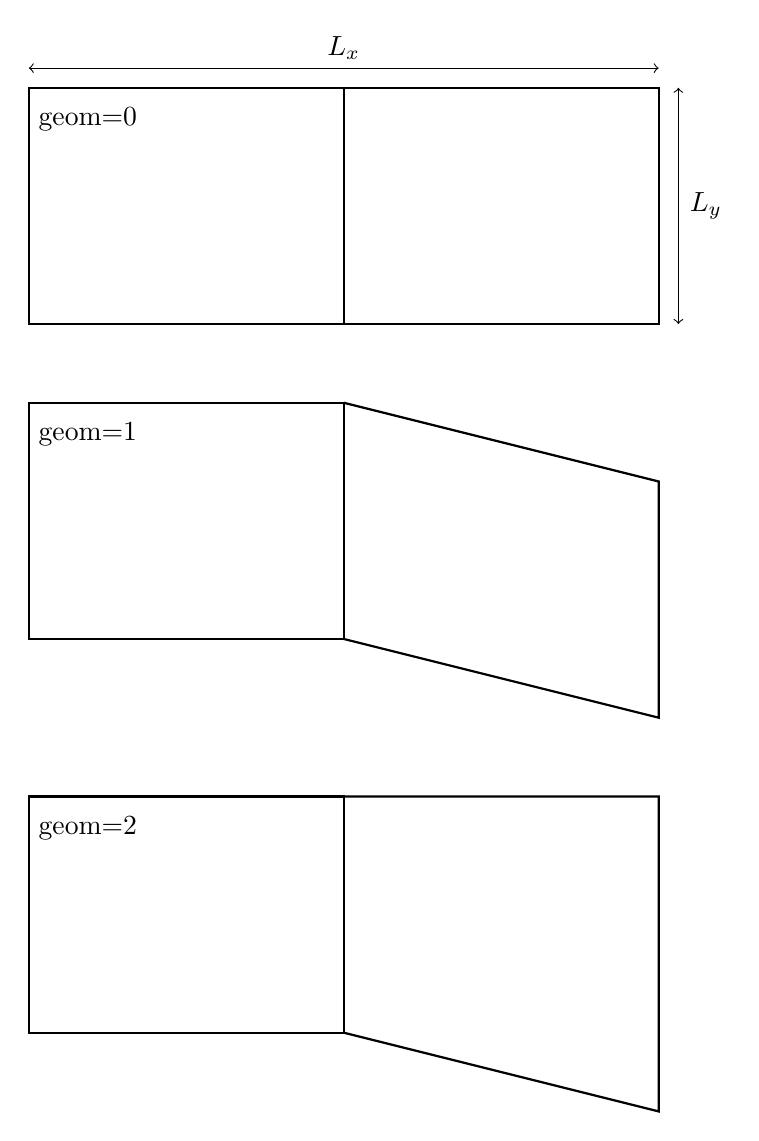
\begin{tikzpicture}
%\draw[step=1cm,gray,very thin] (0,0) grid (10,14); 
\draw[<->,thin] (1,13.25)--(9,13.25);
\node[] at (5,13.5) {$L_x$};
\draw[<->,thin] (9.25,10)--(9.25,13);
\node[] at (9.6,11.5) {$L_y$};
%.............................
\node[] at (1.75,12.6) {geom=$0$};
\draw[thick](1,10) rectangle (5,13); 
\draw[thick](5,10) rectangle (9,13); 
%.............................
\node[] at (1.75,8.6) {geom=$1$};
\draw[thick](1,6) rectangle (5,9);  
\draw[thick](5,6)--(9,5)--(9,8)--(5,9);  
%.............................
\node[] at (1.75,3.6) {geom=$2$};
\draw[thick](1,1) rectangle (5,4);  
\draw[thick](5,1)--(9,0)--(9,4)--(5,4);  
\end{tikzpicture}


\end{center}
and three different elements: ${\bm Q}_1\times P_0$, ${\bm Q}_2\times Q_1$, and ${\bm Q}_3\times Q_2$.

%.............................
\subsubsection*{geom=0}

I find that the checkerboard mode is present for the unstable ${\bm Q}_1\times P_0$
element. However, for all three elements the velocity is zero, down to machine precision.
For the two continuous-pressure elements the pressure at the top is 0 and 6 at the 
bottom as expected.

\begin{center}
\includegraphics[width=5.4cm]{python_codes/fieldstone_42/results/geom0/press1}
\includegraphics[width=5.4cm]{python_codes/fieldstone_42/results/geom0/press2}
\includegraphics[width=5.4cm]{python_codes/fieldstone_42/results/geom0/press3}\\
\includegraphics[width=5.4cm]{python_codes/fieldstone_42/results/geom0/vel1}
\includegraphics[width=5.4cm]{python_codes/fieldstone_42/results/geom0/vel2}
\includegraphics[width=5.4cm]{python_codes/fieldstone_42/results/geom0/vel3}\\
{\captionfont From left to right: ${\bm Q}_1\times P_0$, ${\bm Q}_2\times Q_1$, 
and ${\bm Q}_3\times Q_2$.}
\end{center}


%.............................
\subsubsection*{geom=1}

We find that the checkerboard mode is now absent and velocities are still zero
for all three elements. The pressure is hydrostatic and only depends on the $y$-coordinate.

\begin{center}
\includegraphics[width=5.1cm]{python_codes/fieldstone_42/results/geom1/press1}
\includegraphics[width=5.1cm]{python_codes/fieldstone_42/results/geom1/press2}
\includegraphics[width=5.1cm]{python_codes/fieldstone_42/results/geom1/press3}\\
\includegraphics[width=5.1cm]{python_codes/fieldstone_42/results/geom1/vel1}
\includegraphics[width=5.1cm]{python_codes/fieldstone_42/results/geom1/vel2}
\includegraphics[width=5.1cm]{python_codes/fieldstone_42/results/geom1/vel3}\\
{\captionfont From left to right: ${\bm Q}_1\times P_0$, ${\bm Q}_2\times Q_1$, 
and ${\bm Q}_3\times Q_2$.}
\end{center}

%.............................
\subsubsection*{geom=2}

As in Fortin \& Fortin (1985) we find that the velocity field now showcases 2 ``convection
cells'' for the  ${\bm Q}_1\times P_0$ element (although they have different shapes than 
the ones in their publication) while the velocity remains zero for the other two elements. 

\begin{center}
\includegraphics[width=5.1cm]{python_codes/fieldstone_42/results/geom2/press1}
\includegraphics[width=5.1cm]{python_codes/fieldstone_42/results/geom2/press2}
\includegraphics[width=5.1cm]{python_codes/fieldstone_42/results/geom2/press3}\\
\includegraphics[width=5.1cm]{python_codes/fieldstone_42/results/geom2/vel1}
\includegraphics[width=5.1cm]{python_codes/fieldstone_42/results/geom2/vel2}
\includegraphics[width=5.1cm]{python_codes/fieldstone_42/results/geom2/vel3}\\
{\captionfont From left to right: ${\bm Q}_1\times P_0$, ${\bm Q}_2\times Q_1$, 
and ${\bm Q}_3\times Q_2$.}
\end{center}


On the following figure the root mean square velocity obtained with the 
${\bm Q}_1\times P_0$ element is shown as a function of 
the element size $h$. We find that it decreases quadratically with $h$. 
\begin{center}
\includegraphics[width=6cm]{python_codes/fieldstone_42/results/vrms.pdf}
\end{center}


 %%%%%%%%%%%%%%%%%%%%%%%%%%%%%%%%%%%%%%%%%%%%%%%%%

\newpage %%%%%%%%%%%%%%%%%%%%%%%%%%%%%%%%%%%%%%%%%%%%%%%%%%%%%%%%%%%%%%%%%%%%%%%%%%%%%%%%
\section{{\tt fieldstone\_43}: the rotating cone \label{f43}} %%%%%%%%%%%%%%%%%%%%%%%%%%%
This benchmark originates in \cite{dohu03}. It is also carried out in \cite{bepo10}.
It considers the advection of a product-cosine hill
in a prescribed velocity field. The initial temperature is:
\begin{equation}
T_0(x,y)=
\left\{
\begin{array}{cc}
\frac{1}{4}
\left(1+\cos \pi\frac{x-x_c}{\sigma}\right)
\left(1+\cos \pi\frac{y-y_c}{\sigma}\right)
& \text{if } (x-x_c)^2+(y-y_c)^2\leq \sigma^2 \\
0 & \text{otherwise}
\end{array}
\right.
\end{equation}
The boundary conditions are $T(x,y)=0$ on all four sides of the unit square domain. In what follows we set $x_c=y_c=1/6$ and $\sigma=0.2$.  The velocity field is analytically prescribed: $\vec\upnu=(-(y-y_c),+(x-x_c))$.

In what follows we test the time integration scheme by setting $\alpha_T=1$ (fully implicit formulation), $\alpha=0$ (fully explicit formulation) and $\alpha_T=1/2$ (Crank-Nicolson).  
The timestep is set to $\delta t=2\pi/200$. The density and heat capacity values are set to 1. 
We monitor the minimum and maximum value of the temperature field, as well as the total thermal energy $E_T$ in the system during the 200 time steps ($2\pi$ rotation of the cone):
\[
E_T=\int_\Omega \rho_0 C_p T dV = \int_\Omega T dV = |\Omega| \langle T \rangle 
\qquad
\text{where}
\qquad
\langle T \rangle = \frac{1}{|\Omega|} \int_\Omega T dV
\]
The time evolution of the temperature with the Crank-Nicolson algorithm is shown hereunder:
\begin{center}
a)\includegraphics[width=4.8cm]{python_codes/fieldstone_43/images/crni/velfield}
b)\includegraphics[width=4.8cm]{python_codes/fieldstone_43/images/crni/crnitemp0000}
c)\includegraphics[width=4.8cm]{python_codes/fieldstone_43/images/crni/crnitemp0050}\\
d)\includegraphics[width=4.8cm]{python_codes/fieldstone_43/images/crni/crnitemp0100}
e)\includegraphics[width=4.8cm]{python_codes/fieldstone_43/images/crni/crnitemp0050}
f)\includegraphics[width=4.8cm]{python_codes/fieldstone_43/images/crni/crnitemp0199}\\
{\small a) Velocity field and initial temperature; b,c,d,e,f) Temperature field at timesteps 0,50,100,150,199.} 
\end{center}
Turning now to the statistics, we plot $\min(T)$, $\max(T)$ and $E_T$ as a function of time:
\begin{center}
\includegraphics[width=5cm]{python_codes/fieldstone_43/images/Tmin.pdf}
\includegraphics[width=5cm]{python_codes/fieldstone_43/images/Tmax.pdf}
\includegraphics[width=5cm]{python_codes/fieldstone_43/images/ET.pdf}\\
{\small Time evolution of the min and max temperature and the total energy}
\end{center}
The conclusions are clear: the explicit method diverges quickly and is unusable. The fully implicit and Crank-Nicolson 
method yield similar energy conservation but the fully-implicit showcases a clear loss in maximum temperature as shown in the following figure:
\begin{center}
\includegraphics[width=15cm]{python_codes/fieldstone_43/images/temp}\\
{\small Temperature field after a full rotation with isocontours every 0.1 value.\\ Left: Fully-implicit; Right: Crank-Nicolson}
\end{center}

Finally we can run the experiment (still a $2\pi$ rotation) 
with three different time steps ($\delta t=2\pi/30,2\pi/60,2\pi/120$) 
and we recover very similar results to those presented in \cite{dohu03}:

\begin{center}
\includegraphics[height=8cm]{python_codes/fieldstone_43/images/dohu03}
\includegraphics[height=8cm]{python_codes/fieldstone_43/images/temps_30_60_120}\\
{\small From top to bottom: $\delta t=2\pi/120,2\pi/60,2\pi/30$ with Crank-Nicolson. Left panel is taken from donea \& Huerta \cite{dohu03}}
\end{center}

\begin{center}
\includegraphics[width=5cm]{python_codes/fieldstone_43/images/Tmin_CN.pdf}
\includegraphics[width=5cm]{python_codes/fieldstone_43/images/Tmax_CN.pdf}
\includegraphics[width=5cm]{python_codes/fieldstone_43/images/ET_CN.pdf}\\
{\small Time evolution of the min and max temperature and the total energy obtained with the Crank-Nicolson algorithm for 4 values of the timestep as indicated by the number between parenthesis.}
\end{center}


\begin{center}
\includegraphics[width=3cm]{python_codes/fieldstone_43/images/solution_0000.pdf}
\includegraphics[width=3cm]{python_codes/fieldstone_43/images/solution_0049.pdf}
\includegraphics[width=3cm]{python_codes/fieldstone_43/images/solution_0099.pdf}
\includegraphics[width=3cm]{python_codes/fieldstone_43/images/solution_0149.pdf}
\includegraphics[width=3cm]{python_codes/fieldstone_43/images/solution_0199.pdf}\\
{\small Time evolution of the temperature field for $\delta t=2\pi/200$ with Crank-Nicolson.}
\end{center}

 %%%%%%%%%%%%%%%%%%%%%%%%%%%%%%%%%%%%%%%%%%%%%%%%%



\newpage %%%%%%%%%%%%%%%%%%%%%%%%%%%%%%%%%%%%%%%%%%%%%%%%%%%%%%%%%%%%%%%%%%%%%%%%%%%%%%%%
\section{{\tt fieldstone}: Gravity: buried sphere} %%%%%%%%%%%%%%%%%%%%%%%%%%%%%%%%%%%%%%
Before you proceed further, please read :

\url{http://en.wikipedia.org/wiki/Gravity_anomaly}

\url{http://en.wikipedia.org/wiki/Gravimeter}

Let us consider a vertical domain $Lx \times Ly$ where $L_x=1000km$
and $Ly=500km$. This domain is discretised by means of a grid which counts $nnp= nnx \times nny$ nodes.
This grid then counts $nel=nelx \times nely = (nnx-1)\times(nny-1)$ cells.
The horizontal spacing between nodes is $hx$ and the vertical spacing is $hy$.

\begin{center}
\includegraphics[width=7cm]{/home/cedrict/Desktop/FIELDSTONE/fieldstone/python_codes/gravity_01/images/drawing}
\end{center}

Assume that this domain is filled with a rock type which 
mass density is given by $\rho_{medium}=3000kg/m^3$, 
and that there is a circular inclusion of another rock type  ($\rho_{sphere}=3200kg/m^3$) 
at location ($xsphere$, $ysphere$) of radius $rsphere$.
The density in the system is then given by 
\[
\rho(x,y) = 
\left\{
\begin{array}{l}
\rho_{sphere} \; {\rm  inside \; the\; circle} \\
\rho_{medium} \; {\rm outside \; the\; circle}
\end{array}
\right.
\]

Let us now assume that we place $nsurf$ gravimeters at the surface of the model. These are placed 
equidistantly between coordinates $x=0$ and coordinates $x=Lx$. We will use the arrays $xsurf$ and $ysurf$
to store the coordinates of these locations. 
The spacing between the gravimeters is $\delta_x=Lx/(nsurf-1)$.

At any given point $(x_i,y_i)$ in a 2D space, one can show that 
the gravity anomaly due to the presence of a 
circular inclusion can be computed as follows:
\begin{equation}
g(x_i,y_i)={2 \pi {\cal G} (\rho_{sphere}-\rho_0) R^2}\frac{y_i-y_{sphere}}{(x_i-x_{sphere})^2+(y_i-y_{sphere})^2}
\end{equation}
where $r_{sphere}$ is the radius of the inclusion, $(x_{sphere},y_{sphere})$ 
are the coordinates of the center of the inclusion, and
$\rho_0$ is a reference density.

However, the general formula to compute the gravity anomaly at a given point $(x_i,y_i)$ in space 
due to a density anomaly of any shape is given by:
\begin{equation}
g(x_i,y_i) = 2 {\cal G} \int\int_\Omega \frac{ \Delta \rho(x,y)  (y-y_i)}{(x-x_i)^2 + (y-y_i)^2  } dxdy
\end{equation}
where $\Omega$ is the area of the domain on which the integration is to be carried out. 
Furthermore the density anomaly can be written : $\Delta \rho (x,y)= \rho(x,y)-\rho_0$.
We can then carry out the integration for each cell and sum their contributions:
\begin{equation}
g(x_i,y_i) = 2 {\cal G} \sum_{ic=1}^{nel} \int\int_{\Omega_e} \frac{ (\rho(x,y) -\rho_0)  (y-y_i)}{(x-x_i)^2 + (y-y_i)^2  } dxdy
\end{equation}
where $\Omega_e$ is now the area of a single cell.
Finally, one can assume the density to be constant within each cell so that $\rho(x,y)\rightarrow \rho(ic)$
and $\int\int_{\Omega_e} dx dy \rightarrow hx \times hy$ and then 
\begin{equation}
g(x_i,y_i) = 2 {\cal G} \sum_{ic=1}^{nel} \frac{ (\rho(ic) -\rho_0)  (y(ic)-y_i)}{(x(ic)-x_i)^2 + (y(ic)-y_i)^2  } s_xs_y
\end{equation}

We will then use the array $gsurf$ to store the value of the gravity anomaly 
measured at each gravimeter at the surface. 

\begin{center}
\includegraphics[width=12cm]{/home/cedrict/Desktop/FIELDSTONE/fieldstone/python_codes/gravity_01/solution.pdf}
\end{center}


\paragraph{To go further}

\begin{itemize}
\item explore the effect of the size of the inclusion on the gravity profile.
\item explore the effect of the $\rho_0$ value.
\item explore the effect of the grid resolution.
\item measure the time that is required to compute the gravity. 
How does this time vary with nsurf ? how does it vary when the grid resolution is doubled ?
\item Assume now that $\rho_2<\rho_1$. What does the gravity profile look like ?
\item what happens when the gravimeters are no more at the surface of the Earth but in a satellite ?
\item if you feel brave, redo the whole exercise in 3D...
\end{itemize}

 %%%%%%%%%%%%%%%%%%%%%%%%%%%%%%%%%%%%%%%%%%%%%%%%%%%%

\newpage %%%%%%%%%%%%%%%%%%%%%%%%%%%%%%%%%%%%%%%%%%%%%%%%%%%%%%%%%%%%%%%%%%%%%%%%%%%%%%%%
\section{Problems, to do list and projects for students} %%%%%%%%%%%%%%%%%%%%%%%%%%%%%%%%

\begin{itemize}
\item Darcy flow. redo WAFLE (see http://cedricthieulot.net/wafle.html)
\item carry out critical Rayleigh experiments for various geometries/aspect ratios. Use Arie's notes. 
\item Newton solver
\item Corner flow 
\item elasticity with markers
\item Indentor/punch with stress b.c. ?
\item chunk grid
\item read in crust 1.0 in 2D on chunk
\item compute gravity based on tetrahedra
\item compare Q2 with Q2-serendipity
\item NS a la http://ww2.lacan.upc.edu/huerta/exercises/Incompressible/Incompressible\_Ex2.htm
\item produce example of mckenzie slab temperature
\item write about impose bc on el matrix
\item constraints
\item discontinuous galerkin
\item formatting of code style
\item navier-stokes ? (LUKAS) use dohu matlab code
\item nonlinear poiseuille
\item Finish nonlinear cavity case5.
\item write about mappings 
\item write about stream functions 
\item free surface 
\item zaleski disk advection
\item better yet simple matrix storage ?
\item write Scott about matching compressible2 setup with his paper
\item deal with large matrices. 
\item compositions, marker chain
\item free-slip bc on annulus and sphere . See for example p540 Gresho and Sani book.
\item non-linear rheologies (two layer brick spmw16, tosn15) 
\item Picard vs Newton
\item including phase changes (w. R. Myhill)
\item compute strainrate in middle of element or at quad point for punch?
\item GEO1442 code 
\item GEO1442 indenter setup in plane ?
\item in/out flow on sides for lith modelling
\item Fehlberg RK advection
\item redo puth17 2 layer experiment
\item create stone for layeredflow (see folder one up)
\item SIMPLE a la p667 \cite{john16} 
\item implement mms5 \ref{mms5}
\item implement/monitor div v
\item shape fct, trial fct, basis fct vs test fct doc
\item Delaunay triangulation, Voronoi, stripack
\end{itemize}

How to deal with large sparse matrices in Python?!!
\begin{verbatim}
a_mat = lil_matrix((Nfem,Nfem),dtype=np.float64)
a_mat=a_mat.tocsr()
sol = spsolve(sps.csr_matrix(a_mat),rhs)
\end{verbatim}
 %%%%%%%%%%%%%%%%%%%%%%%%%%%%%%%%%%%%%%%%%%%%%%%%%%%%%%%%%%%%%%%%%%%%%%%%

\appendix %========================================================================================

\newpage %%%%%%%%%%%%%%%%%%%%%%%%%%%%%%%%%%%%%%%%%%%%%%%%%%%%%%%%%%%%%%%%%%%%%%%%%%%%%%%%
%%%%%%%%%%%%%%%%%%%%%%%%%%%%%%%%%%%%%%%%%%%%%%%%%%%%%%%%%%%%%%%%%%%%%%%%%%%%%%%%%%%%%%%%%
\section{Three-dimensional applications} 
In the following table I list many papers which showcase high-resolution models of 
geodynamical processes (subduction, rifting, mantle flow, plume transport, ...).
Given the yearly output of our community and the long list of journal in which 
research can be disseminated, this list can not be exhaustive.

\begin{tabular}{lll}
\hline
Author(s)     & topic   & resolution \\
\hline
\hline
\cite{baih10} & Small-scale sublithospheric convection in the Pacific                           & $448\times56\times64$ \\ 
\cite{stsf10} & Migration and morphology of subducted slabs in the upper mantle                 & $50\times50\times25$ \\
\cite{pyeg10} & Subduction scissor across the South Island of New Zealand                       & $17\times9\times9$ \\
\cite{mamb10} & Influence of a buoyant oceanic plateau on subduction zones                      & $80\times 40 \times80$ \\%(256,000 elts) \\
\cite{cafz11} & Subduction dynamics, origin of Andean orogeny and the Bolivian orocline         & $96\times96\times64$ \\%(590,000 elts) \\
\cite{ellw11} & Feedback between rifting and diapirism, ultrahigh-pressure rocks exhumation     & $100\times64\times20$ \\%\\($128,000$ elts) \\
\cite{alht11} & Numerical modeling of upper crustal extensional systems                         & $160\times160\times12$ \\%(307,200 elts) \\
\cite{alht12} & Rift interaction in brittle-ductile coupled systems                             & $160\times160\times23$ \\%(588,800 elts) \\
\cite{lehm12} & Kinematic interpretation of the 3D shapes of metamorphic core complexes         & $67\times67\times33$ \\%(150,000 elts)  \\
\cite{jabi12} & Role of rheology and slab shape on rapid mantle flow: the Alaska slab edge      & $960\times648\times160$ \\%(99,000,000 elts)$^1$ \\
\cite{cafa12} & Complex mantle flow around heterogeneous subducting oceanic plates              & $96\times96\times64$ \\%(590,000 elts) \\
\cite{brps12} & Oblique rifting and continental break-up                                        & $150\times50\times30$ \\%(225,000 elts) \\
\cite{bemm13} & Influence of mantle plume head on dynamics of a retreating subduction zone      & $80\times40\times80$\\% (256,000 elts \\
\cite{brau13} & Rift to break-up evolution of the Gulf of Aden                                  & $83\times83\times40$\\% (275,560 elts) \\
\cite{brps13} & Thermo-mechanical impact of plume arrival on continental break-up               & $100\times70\times20$\\% (140,000 elts) \\
\cite{care13} & Subduction and slab breakoff controls on Asian indentation tectonics            & $96\times96\times64$\\% (589,824 elts) \\
\cite{faca13} & Modeling of upper mantle deformation and SKS splitting calculations             & $96\times64\times96$ \\% (589,824 elts) \\
\cite{scmo13} & Backarc extension/shortening, slab induced toroidal/poloidal mantle flow        & $352\times 80 \times64$ \\%(1,802,240 elts) \\
\cite{magc13} & Sediment transports in the context of oblique subduction modelling              & $500\times 164\times 100$\\% (8,200,000 cells) \\
\cite{zhgt13} & Crustal growth at active continental margins                                    & $404\times164\times100$ \\%(6,625,600 cells) \\
\cite{lesh13} & Dynamics of India-Asia collision                                                & $257\times257\times 33$\\% (262,144 Q2P-1 elts) \\
\cite{whbb14} & Strain-partitioning in the Himalaya                                             & $256\times256\times40$ \\%(2,621,440 elts) \\
\cite{lixg13} & Collision of continental corner from 3-D numerical modeling                     & $500 \times 340 \times 164$ \\%(27,880,000 cells) \\
\cite{puge14} & Dependence of mid-ocean ridge morphology on spreading rate                      & $196\times196\times100$ \\%(3,841,600 cells)  \\
\cite{facc14} & Mid mantle seismic anisotropy around subduction zones                           & $197\times197\times53$ \\% (1,997,632 cells) \\
\cite{hebr14} & Oblique rifting of the Equatorial Atlantic                                      & $120\times80\times20$ \\%(192,000 elts) \\
\cite{mobm14} & Dynamics of continental accretion                                               & $256\times96\times96$ \\
\cite{rugb14} & Thrust wedges: infl. of decollement strength on transfer zones                  & $309\times85\times149$\\
\cite{buge14} & Asymmetric three-dimensional topography over mantle plumes                      & $500\times500\times217$ \\
\cite{thsh14} & modelled crustal systems undergoing orogeny and subjected to surface processes  & $96\times32\times14$\\
\cite{lige14b}& Thermo-mechanical modeling ontinental rifting and seafloor spreading            & $197\times197\times197$  \\ 
\hline
\end{tabular}



 %%%%%%%%%%%%%%%%%%%%%%%%%%%%%%%
\newpage %%%%%%%%%%%%%%%%%%%%%%%%%%%%%%%%%%%%%%%%%%%%%%%%%%%%%%%%%%%%%%%%%%%%%%%%%%%%%%%%
\section{Codes in geodynamics \label{app:codes} }
In what follows I make a quick inventory of the main codes of computational geodynamics, 
for crust, lithosphere and/or mantle modelling.

in order to find all CIG-codes citations go to: https://geodynamics.org/cig/news/publications-refbase/

\begin{itemize}

%------------
\item ABAQUS

\cite{gedh02}
\cite{fumr03}
\cite{camg07}
\cite{kuhe09}
\cite{camg10}
\cite{makh09}
\cite{nalr12}
\cite{pevp15}


%------------
\item ADELI

\noindent
1997: \cite{hajc97}\\
2004: \cite{gocl04}\\
2006: \cite{vech06} \\
2008: \cite{boht08a}\cite{boht08b}\\
2012: \cite{gech12}\cite{gigh12}\\
2013: \cite{wahd13}\\
2015: \cite{ceag15}\\
2018: \cite{cegm18}\cite{gehn18}

%------------
\item ASPECT

This code is hosted by CIG at \url{https://geodynamics.org/cig/software/aspect/}. 
It is an open source community code based on the finite element library deal.II. 
It is massively parallel, relies on the p4est library for adaptive mesh refinement,
uses the Trilinos solver library, and can deal with 2D and 3D geometries. 

\cite{bahk07}
\cite{krhb12}
\cite{aupm15}
\cite{tosn15}
\cite{dahe16}
\cite{gadb16}
\cite{zhon16}
\cite{hepb17}
\cite{daef17}
\cite{hedg17}
\cite{robh17}
\cite{robu17}
\cite{aumh17}
\cite{thie17}
\cite{brsg17}
\cite{onmz17}
\cite{tasm17}
\cite{zhli17}
\cite{daga18}
\cite{onzh18}
\cite{gltf18}
\cite{heps18}
\cite{galh18}
\cite{peka18}
\cite{puth18}
\cite{brst18b}
\cite{baba19}
\cite{stbl19}
\cite{cocf19}
\cite{liki19}

%-------------
\item BASIL/ELLE \url{http://elle.ws/}
\cite{bokj08}
\cite{llor19}

%------------
\item CHIC 
\cite{norv15}

%------------
\item CitcomS and CITCOMCU

These codes are hosted by CIG at \url{https://geodynamics.org/cig/software/citcomcu/}
and \url{https://geodynamics.org/cig/software/citcoms/}.

\noindent
1996: \cite{somo96}\\
1997: \cite{mole97}\\
1998: \cite{moso98}\cite{zhgm98}\cite{vazh99}\\
2000: \cite{zhzm00}\cite{gumr00}\\
2001: \cite{bigu01}\\
2002: \cite{tagh02}\\
2003: \cite{vazh03}\cite{cogu03}\cite{bigu03}\\
2004: \cite{solo04}\\
2005: \cite{bihi05}\\
2006: \cite{beck06}\cite{pibf06}\cite{tact06}\cite{besb06}\cite{coli06}\\
2007: \cite{bihi07}\cite{zhzl07}\cite{magu07}\cite{bavi07}\cite{rimb07}\cite{mofm07}\cite{cobs07}\\
2008: \cite{dihf08}\cite{gamc08}\cite{zhmt08}\cite{hole08}\\
2009: \cite{lizh09}\cite{arhm09}\cite{zhzm09}\cite{anbi09}\cite{fobe09}\cite{bubi09}\cite{befa09}\cite{lezh09}\\
2010: \cite{bumb10}\cite{vabv10}\cite{baiv10}\cite{bubi10}\cite{zhzl10}\cite{bill10}\cite{jabi10}\\
2011: \cite{befa11}\cite{lemj11}\cite{vaal11}\cite{legu11}\cite{list11}\\
2012: \cite{arbi12}\cite{jabi12}\cite{bija12}\cite{bova12}\cite{hucf12}\cite{zhym12}\cite{solo12}
\cite{hibi12}\cite{jabk12}\cite{mapm12}\\
2013: \cite{bacs13}\cite{bogs13a}\cite{bogs13b}\cite{jabr13}\cite{qula13}\cite{oldh13}\cite{arbi13}\cite{cost13}\\
2014: \cite{flgw14}\cite{budt14}\cite{kava14}\cite{arfw14}\cite{wavp14}\cite{seki14}\cite{agvg14}
\cite{mabv14}\cite{zhu14}\\
2015: \cite{bacs15}\cite{bogf15}\cite{bomv15}\cite{sefw15}\cite{daso15}\cite{vami15}\cite{wazh15}
\cite{wavp15}\cite{waav15}\cite{hafg15}\cite{tarn15}\cite{legu15}\\
2016: \cite{welm16}\cite{wele16}\cite{jada16}\cite{frbs16}\\
2017: \cite{aggv17}\cite{maav17}\cite{frbm17}\cite{haja17}\\
2018: \cite{hect18}\cite{king18}\cite{kavb18}\\
2019: \cite{mavb19}\cite{fube19}\cite{magn19}\cite{malg19}\cite{mazh19}


\todo[inline]{cross check with CIG database}


%------------
\item CONMAN
This code is hosted by CIG at \url{https://geodynamics.org/cig/software/conman/}

\cite{kirh90}
\cite{itki94}
\cite{kian95}
\cite{kian98}
\cite{itki98}
\cite{befo99}
\cite{nake07}
\cite{dadh07}
\cite{kifr15}


%------------
\item CONVRS 
\cite{yoth12}
\cite{yosh13} 
 



%------------
\item DOUAR

\cite{brtf08}
\cite{thfb08}
\cite{yahb09}
\cite{brya10}
\cite{lobh10}
\cite{mutg13}
\cite{whbb14}
\cite{neew18}
\cite{koen19}

%------------
\item DYNEARTHSOL
\cite{chtl13}


\item ELMER
Elmer is an open source multiphysical simulation software mainly developed by 
CSC - IT Center for Science (CSC). Elmer development was started 1995 in collaboration with 
Finnish Universities, research institutes and industry. Elmer includes physical models of 
fluid dynamics, structural mechanics, electromagnetics, heat transfer and acoustics, 
for example. These are described by partial differential equations which Elmer solves 
by the Finite Element Method (FEM). \url{https://www.csc.fi/web/elmer}

\cite{mals14}


%------------
\item M-DOODS, Duretz code
\cite{yatd12}
\cite{yahb13}
\cite{chmd19}

%------------
\item FENICS
\cite{alrk14}


%------------
\item GAIA

\cite{hutm13}

%------------
\item GALE

This code is hosted by CIG at \url{https://geodynamics.org/cig/software/gale/}

\cite{fabs08}
\cite{gotc08}
\cite{beve10}
\cite{cmwt10}
\cite{lehm12}\cite{liqi12}
\cite{arbi13}

%------------
\item (G)TECTON

\noindent
1980: \cite{mera80}\\
1981: \cite{mera81}\\
1993: \cite{gowo93}\\
1995: \cite{gowo95}\\
1996: \cite{guez96}\\
1999: \cite{gowo99}\\
2001: \cite{bugw01}\cite{gome01}\\
2002: \cite{bugw02}\\
2005: \cite{gowo05}\cite{vanw05}\cite{vabl05}\\
2006: \cite{degw06}\cite{libi06}\cite{scdm06}\\
2007: \cite{vabl07}\\
2009: \cite{ladg09}\\
2011: \cite{bagw11}\cite{bagw11b}\\
2015: \cite{mags15}

%------------
\item ELEFANT

\cite{tosn15}
\cite{matv15}
\cite{busa16}
\cite{latb17}
\cite{thie17}
\cite{pltv18}
\cite{wohu19}

%-------------
\item ELLIPSIS

\cite{modm03}
\cite{omma06} 
\cite{moql07}
\cite{dyrm07}
\cite{onlg08}
\cite{pyeg10}
\cite{legu11}
\cite{lega12}


%------------
\item FANTOM
\index{FANTOM}

\cite{thie11}
\cite{alht11}
\cite{alht12}
\cite{alhf13}
\cite{erhv14}
\cite{thsh14}
\cite{erhv15}
\cite{erhv19}

%------------
\index FDCON

\cite{enbs05}
\cite{fusc13}
\cite{fuks15}


%------------
\index{FLUIDITY}
\item FLUIDITY
\cite{dawk11}
\cite{gagd14}

\index{geoFLAC}
\item geoFLAC (based on PARAVOZ)
\cite{jala19}

%------------
\index{IFISS}
\item IFISS: Incompressible Flow Iterative Solution Solver is a
MATLAB package that is a very useful tool for people interested in
learning about solving PDE’s.
IFISS includes built-in software for 2D versions of:
the Poisson equation, the convection-diffusion equation, the Stokes equations
and the Navier-Stokes equations.\\
\url{https://personalpages.manchester.ac.uk/staff/david.silvester/ifiss/}



%------------
\item the I2(3)E(L)VIS code

2003: \cite{geyu03}\cite{geyu03b}\cite{geur03}\\
2004: \cite{geym04}\cite{geys04}\cite{gepm04}\\
2005: \cite{buge05}\\
2006: \cite{bbeg06}\cite{gest06}\cite{gogc06}\cite{gecy06}\\
2007: \cite{geyu07}\cite{gogc07}\\
2008: \cite{scbe08}\cite{gecy08}\cite{uegs08}\cite{fagc08}\cite{zhgy09}\\
2009: \cite{gefc09}\\
2010: \cite{gerya2010}\cite{nigm10}\\
2011: \cite{dugm11}\cite{dumg11}\cite{lixg11}\cite{gery11}\cite{geme11}\\
2012: \cite{crsg12}\cite{dugk12}\cite{lixg12}\cite{fagm12}\\
2013: \cite{lixg13}\cite{nabg13}\cite{magc13}\cite{vagd13a}\cite{vagd13b}\cite{zhgt13}\cite{dyge13}\cite{gemd13}\cite{mana13}\\
2014: \cite{dugs14}\cite{puge14}\cite{rugb14}\cite{voge14b}\cite{bagb14}\cite{lige14}\cite{stjm14}\cite{malg14}
\cite{buge14}\cite{gosk14}\cite{bagb14}\cite{vamd14}\\
2015: \cite{duay15}\cite{uewg15}\cite{rula15}\cite{gesb15}\cite{rula15}\\
2016: \cite{kobc16}\cite{magc16}\cite{fige16}\\
2019: \cite{kobg19}\cite{ligc19}

%------------
\item I3MG
\cite{facc14}

%------------
\item LAMEM
\cite{scbe08}
\cite{kamm10}
\cite{lemk11}
\cite{may12}
\cite{lesh14}
\cite{cokm14}
\cite{bakp14}
\cite{feka14a}
\cite{feka14b}
\cite{puka15}
\cite{feka15}
\cite{cofk15}
\cite{kapb16}

%------------
\item LAPEX2D (LAgrangian Particle EXplicit, based on the prototype code PAROVOZ) 
\cite{sopg05}
\cite{bbeg06}\cite{basv06}
\cite{baso08}
\cite{scbe08}
\cite{sosk11}


%-------------
\item LITMOD
\cite{afrf07}
\cite{affr08}
\cite{fuac09}
\cite{fufa10}


%------------
\item MARC
\cite{nesg97}
\cite{nesb99}


%------------
\item MILAMIN

MILAMIN is a finite element method implementation in native MATLAB that is capable of doing one million degrees of freedom per minute on a modern desktop computer. This includes pre-processing, solving, and post-processing. The MILAMIN strategies and package are applicable to a broad class of problems in Earth science. \url{http://milamin.org/}

\noindent
2008: \cite{daks08}\\
2010: \cite{krda10}\cite{kaus10}\\
2011: \cite{yakm11}\\
2012: \cite{gebk12}\\
2014: \cite{jobk14}\\
2015: \cite{lukz15}\cite{gehm15}\cite{thkp15}\cite{musd15}\\
2016: \cite{jads16}\cite{maka16}\\
2018: \cite{dusd18}\cite{jasc18}\cite{jadg18}\cite{comj18}\cite{jens18}\cite{rabw18}\cite{chsm18}\\
2019: \cite{anpa19}\cite{sifg19}\cite{baba19}


%------------
\item PARAVOZ/FLAMAR/FLAC

\noindent
1989: \cite{cund89}\\
1993: \cite{poli93}\\
1996: \cite{hach96}\\
1998: \cite{gepd98}\\
2000: \cite{labp00}\\
2001: \cite{bujl01}\cite{bupo01}\\
2002: \cite{bast02}\cite{clbb02}\\
2003: \cite{hags03}\cite{gehd03}\cite{upke03}\\
2004: \cite{guhl04}\cite{gewi04}\cite{toba04}\cite{tibb04}\\
2005: \cite{bugu05}\\
2007: \cite{yaab07}\cite{buto07}\\
2008: \cite{yaba08}\cite{tibb08}\\
2009: \cite{gecm09}\cite{yahb09}\cite{bucl09}\\
2012: \cite{anwb12}\cite{gech12}\cite{gubc12}\cite{gerb12}\\
2013: \cite{wabd13}\cite{frbm13}\\
2014: \cite{frba14}\cite{gagb14}\cite{bufa14}\\
2015: \cite{wulc15}\cite{marl15}\cite{gebw15}\cite{svlh15}\\




%------------
\item PINK3D
\cite{vosc15}


%------------
\item PLASTI
\cite{fuwb06}



%------------
\item pTatin3D: A nice succinct description of the code is given in Appendix B of \cite{lemh17}.

2013: \cite{phil13}\\
2014: \cite{mabl14}\\
2015: \cite{mabl15}\\
2017: \cite{lemh17}\\
2018: \cite{jolp18}\\
2019: \cite{jolm19}

%---------------------
\item Pylith

\cite{aakw13}


%------------
\item RHEA
\cite{bugg08}
\cite{stgb10}
\cite{algs12}
\cite{busa13}

%------------
\item SAMOVAR
\cite{egat10}

%------------
\item SEPRAN

1993: \cite{beky93}\cite{vavy93}\\
1994: \cite{vlvv94}\cite{vayv94}\\
1995: \cite{vayv95}\\
1996: \cite{vayu96}\\
2002: \cite{civv02}\cite{vavv02}\\
2003: \cite{vavs03}\\
2004: \cite{vavv04}\cite{vavv04b}\cite{vavv04c}\\
2005: \cite{vavv05}\cite{sepr05}\\
2006: \cite{liva06a}\cite{liva06b}\\
2007: \cite{vant07}\cite{civv07}\cite{brva07a}\cite{brva07b}\\
2008: \cite{plva08}\\
2009: \cite{vavl09}\\
2010: \cite{vahy10}\cite{syva10}\\
2011: \cite{vahs11}\\
2012: \cite{besy12}\cite{beva12}\cite{chgv12}\\
2013: \cite{ancv13}\\
2014: \cite{chsg14}\cite{mova14}\\
2015: \cite{vasy15}\\
2019: \cite{zhdv19}\cite{vayu19}

%------------
\item SISTER

\cite{olbm16}

%------------
\item SLIM3D

\cite{poso08}
\cite{qusp10}
\cite{brps12}
\cite{brps13}
\cite{brau13}
\cite{brun14}
\cite{hebr14}
\cite{kobf14}
\cite{clbq15}
\cite{brcr17}
\cite{basq18}

%------------
\item SLOMO
\cite{kaus05}

%------------
\index SNAC
\cite{chlg08}


%------------
\item SOPALE

1994: \cite{wibe94}\cite{befh94}\\
1995: \cite{full95}\cite{elfb95}\\
1996: \cite{bekh96}\\
1999: \cite{will99a}\cite{will99b}\\
2000: \cite{pybf00}\cite{bemh00}\\
2001: \cite{bejn01}\\
2002: \cite{hube02}\cite{pybf02}\\
2003: \cite{hube03}\cite{vamf03}\cite{wipo03}\cite{pymi03}\\
2004: \cite{bejn04}\cite{pycr04}\cite{pybe04}\cite{elsp04}\cite{geim04}\\
2005: \cite{gebi05}\cite{hubb05}\\
2006: \cite{pysk06}\cite{selz06}\\
2007: \cite{hube07}\cite{cubh07}\cite{mohb07}\\
2008: \cite{sebp08}\cite{wabj08}\cite{wabj08b}\cite{gopy08}\\
2009: \cite{kecw09}\cite{bejb09}\cite{bupb09}\cite{grba09}\cite{sihb09}\\
2010: \cite{albs10}\cite{albe10}\cite{grpy10}\cite{pygp10}\\
2011: \cite{cube11}\cite{bubj11}\cite{hube11}\\
2012: \cite{grpy12}\cite{grpy12b}\cite{kogp12}\cite{grbe12}\cite{jahu12}\\
2013: \cite{bubj13}\cite{chbe13}\cite{fihv13a}\cite{fihv13b}\cite{gobi13}\cite{grpy13}\cite{knak13}\cite{nipc13}\cite{jahm13}\\
2014: \cite{gogu14}\\
2015: \cite{albe15}\cite{bubj15}\cite{heps15}\\
2016: \cite{licu16}\\
2017: \cite{bube17}


%------------
\item STAGYY
\cite{rota11}
\cite{yadl14}
\cite{crta14}
\cite{cosh18}
\cite{gult19}

%------------
\item SUBMAR

\cite{masr06}
\cite{masp07}
\cite{roms10}


%------------
\item SULEC
SULEC is a finite element code that solves the incompressible Navier-Stokes equations 
for slow creeping flows. The code is developed by Susan Ellis 
(GNS Sciences, NZ) and Susanne Buiter (NGU). 
\url{http://www.geodynamics.no/buiter/sulec.html}

\noindent
2011: \cite{qube11}\cite{ellw11}\\
2012: \cite{buit12}\cite{tebu12}\cite{crsg12}\cite{grel12}\\
2013: \cite{ghbu13}\\
2014: \cite{ghbu14}\cite{qubu14}\\
2015: \cite{nabu15}\\
2016: \cite{zwsn16}\\
2017: \cite{nabp17}\\
2018: \cite{tebu18}











%------------
\item TERRA:
The computational grid is based on a projection of the regular icosahedron onto a 
sphere and successive dyadic refinements \cite{bafr85}.  Concentric copies of such  
spherical layers of nodes build the domain in radial direction.

\cite{baum83}
\cite{glat88}
\cite{buba95}
\cite{burb97}\cite{yang97}
\cite{burl98}
\cite{phbs09}\cite{wodd09}\cite{gows09}
\cite{woda11}
\cite{dadb13}
\cite{vade16}

\index{TerraFERMA}
\item TerraFERMA
\cite{wisv14}
\cite{wisv17}
\cite{spmw16}
\cite{ceww17}
\cite{ceww19}


%------------
\item YACC
\cite{tosn15}
\cite{tomy16}

%------------
\item UNDERWORLD 1\&2

\noindent
2006: \cite{stfs06}\\
2007: \cite{moql07}\cite{stfs07}\\
2008: \cite{lemm08}\cite{ozrs08}\cite{gotc08}\\
2010: \cite{casm10}\cite{mamb10}\cite{stsf10}\cite{stfc10}\cite{fasm10}\\
2011: \cite{memm11}\cite{cafz11}\\
2012: \cite{cafa12}\\
2013: \cite{bemm13}\cite{scmo13}\cite{faca13}\cite{care13}\\
2014: \cite{famc14}\\
2015: \cite{quxm15}\cite{bemm15}\cite{scsp15}\cite{shmj15}\\
2016: \cite{shmv16}\cite{onlw16}\cite{kicf16}\\
2018: \cite{memm18}\\
2019: \cite{samo19}\cite{yamg19}

\item VEMAN
\cite{bepo10}


\end{itemize}
 %%%%%%%%%%%%%%%%%%%%%%%%%%%%%%
\newpage %%%%%%%%%%%%%%%%%%%%%%%%%%%%%%%%%%%%%%%%%%%%%%%%%%%%%%%%%%%%%%%%%%%%%%%%%%%%%%%%
\section{Matrix properties} \subsection{Symmetric matrices}

Any {\sl symmetric} matrix 
has only real eigenvalues,
is always diagonalizable,
and has orthogonal eigenvectors.
A symmetric $N\times N$ real matrix ${\bm M}$ is said to be
\begin{itemize}
\item {\bf positive definite} if $\vec x \cdot {\bm M} \cdot \vec x >0$ for every non-zero vector $\vec x$ of n real numbers. All the eigenvalues of a  Symmetric Positive Definite (SPD) matrix are positive.
 If A and B are positive definite, then so is A+B.
The matrix inverse of a positive definite matrix is also positive definite.
An SPD matrix has a unique Cholesky decomposition. In other words the matrix ${\bm M}$ 
is positive definite if and only if there exists a unique
lower triangular matrix ${\bm L}$, with real and strictly positive diagonal elements, 
such that ${\bm M} = {\bm L}{\bm L}^T$
(the product of a lower triangular matrix and its conjugate transpose).
This factorization is called the Cholesky decomposition of ${\bm M}$.
\index{general}{Symmetric Positive Definite}

\item {\bf positive semi-definite} if $\vec x \cdot {\bm M} \cdot  \vec x \geq 0$
\item {\bf negative definite} if $\vec x \cdot {\bm M} \cdot \vec x < 0$
\item {\bf negative semi-definite} if $\vec x \cdot {\bm M} \cdot \vec x \leq 0$
\end{itemize}

The Stokes linear system
\[
\left( \begin{array}{cc}
\mathbb{K} & \mathbb{G}  \\ \mathbb{G}^T &  0
\end{array} \right) \cdot
\left( \begin{array}{c}  {\bm v} \\ {\bm p}  \end{array} \right) = 
\left( \begin{array}{c}  {\bm f} \\ {\bm g}  \end{array} \right) 
\]
is {\bf indefinite} (i.e. it has positive as well as negative eigenvalues).

A square matrix that is not invertible is called {\bf singular} or degenerate. A square matrix is singular if and only if its determinant is 0. Singular matrices are rare in the sense that if you pick a random square matrix, it will almost surely not be singular.

%--------------------------------
\subsection{Schur complement}

From wiki.
In linear algebra and the theory of matrices, the Schur complement of a matrix block (i.e., a submatrix within a larger matrix) is defined as follows.
Suppose ${\bm A}$, ${\bm B}$, ${\bm C}$, ${\bm D}$
are respectively $p\times p$, $p \times q$, $q \times p$ and $q \times q$ matrices, and $\mathbb{D}$ is invertible. Let
\[
{\bm M}=
\left( \begin{array}{cc}
{\bm A} & {\bm B}  \\ 
{\bm C} & {\bm D}
\end{array} \right) 
\]
so that ${\bm M}$ is a $(p+q)\times(p+q)$ matrix.
Then the Schur complement of the block ${\bm D}$ of the matrix ${\bm M}$ is the $p \times p$ matrix
\[
{\bm S}={\bm A}-{\bm B}\cdot {\bm D}^{-1}\cdot {\bm C}
\]
Application to solving linear equations: The Schur complement arises naturally 
in solving a system of linear equations such as
\begin{eqnarray}
{\bm A}\cdot\vec x+{\bm B}\cdot \vec y &=& \vec f \nonumber\\
{\bm C}\cdot\vec x+{\bm D}\cdot \vec y &=& \vec g \nonumber
\end{eqnarray}
where $\vec x$, $\vec f$ are $p$-dimensional vectors, $\vec y$, $\vec g$
are $q$-dimensional vectors,
and ${\bm A}$, ${\bm B}$, ${\bm C}$, ${\bm D}$ are as above.
Multiplying the bottom equation by ${\bm B}\cdot {\bm D}^{-1}$ 
and then subtracting from the top equation one obtains
\[
({\bm A}-{\bm B}\cdot {\bm D}^{-1}\cdot {\bm C})\cdot \vec x = \vec f - {\bm B}\cdot {\bm D}^{-1}\cdot \vec g
\]
Thus if one can invert ${\bm D}$ as well as the Schur complement of ${\bm D}$, one can solve for $\vec x$,
and then by using the equation $\bm C\cdot \vec x + \bm D \cdot \vec y = \vec g$ one can solve for $y$.
This reduces the problem of inverting a $(p+q) \times (p+q)$ matrix to that of inverting
a $p \times p$ matrix and a $q \times q$ matrix.
In practice one needs ${\bm D}$ to be well-conditioned in order for 
this algorithm to be numerically accurate.

Considering now the Stokes system: 
\[
\left( \begin{array}{cc}
\K & \G  \\ \G^T &  -\C
\end{array} \right) \cdot
\left( \begin{array}{c}  {\vec v} \\ {\vec p}  \end{array} \right) = 
\left( \begin{array}{c}  {\vec f} \\ {\vec g}  \end{array} \right) 
\]
Factorising for ${\vec p}$ we end up with a {\bf velocity-Schur complement}.
Solving for ${\vec p}$ in the second equation and inserting the expression
for ${\vec p}$ into the first equation we have
\[
\mathbb{S}_v \cdot {\vec v}  = {\vec f} 
\quad\quad
\text{with}
\quad\quad
\mathbb{S}_v=\K+ \G \cdot \C^{-1} \cdot \G^T
\]
Factorising for $\vec v$ we get a {\bf pressure-Schur complement}.
\[
\mathbb{S}_p \cdot {\vec p}  = \G^T \cdot \K^{-1}\cdot {\vec f}
\quad\quad
\text{with}
\quad\quad
\mathbb{S}_p = \G^T \cdot \K^{-1}\cdot \G + \C 
\]


 %%%%%%%%%%%%%%%%%%%%%%%%%%%%%%%%%%%%%%%%%%%%
\newpage %%%%%%%%%%%%%%%%%%%%%%%%%%%%%%%%%%%%%%%%%%%%%%%%%%%%%%%%%%%%%%%%%%%%%%%%%%%%%%%%
\section{Don’t be a hero - unless you have to} What follows was published online on July 17th, 2017 at 
\url{https://blogs.egu.eu/divisions/gd/2017/07/19/dont-be-a-hero-unless-you-have-to/}
It was written by me and edited by Iris van Zelst, at the time PhD student at ETH Z\"urich.

\vspace{3mm}

In December 2013, I was invited to give a talk about the \aspect{} code [1] 
at the American Geological Union conference in San Francisco. Right 
after my talk, Prof. Louis Moresi took the stage and gave a talk entitled: 
{\it Underworld: What we set out to do, How far did we get, What did we Learn?}

The abstract went as follows:

"Underworld was conceived as a tool for modelling 3D lithospheric deformation coupled with the underlying / surrounding mantle flow. The challenges involved were to find a method capable of representing the complicated, non-linear, history dependent rheology of the near surface as well as being able to model mantle convection, and, simultaneously, to be able to solve the numerical system efficiently. […] The elegance of the method is that it can be completely described in a couple of sentences. However, there are some limitations: it is not obvious how to retain this elegance for unstructured or adaptive meshes, arbitrary element types are not sufficiently well integrated by the simple quadrature approach, and swarms of particles representing volumes are usually an inefficient representation of surfaces."

Aside from the standard numerical modelling jargon, Louis used a term during his talk which I thought at the time had a nice ring to it: hero codes. In short, I believe he meant the codes written essentially by one or two people who at some point in time spent great effort into writing a code (usually choosing a range of applications, a geometry, a number of dimensions, a particular numerical method to solve the relevant PDEs(1), and a tracking method for the various fields of interest).

In the long list of Hero codes, one could cite (in alphabetical order) CITCOM [1], \douar [8], \fantom [2], IELVIS [5], LaMEM [3], pTatin [4], SLIM3D [10], \sopale [7], StaggYY [6], \sulec [11], Underworld [9], and I apologise to all other heroes out there whom I may have overlooked. And who does not want to be a hero? The Spiderman of geodynamics, the Superwoman of modelling?

Louis' talk echoed my thoughts on two key choices we (computational geodynamicists) are facing: Hero or not, and if yes, what type?

\vspace{3mm}

{\bf Hero or not?}

\vspace{3mm}

Speaking from experience, it is an intense source of satisfaction when peer-reviewed published results are obtained with the very code one has painstakingly put together over months, if not years. But is it worth it?

On the one hand, writing one own’s code is a source of deep learning, a way to ensure that one understands the tool and knows its limitations, and a way to ensure that the code has the appropriate combination of features which are necessary to answer the research question at hand. On the other hand, it is akin to a journey; a rather long term commitment; a sometimes frustrating endeavour, with no guarantee of success. Let us not deny it – many a student has started with one code only to switch to plan B sooner or later. Ultimately, this yiels a satisfactory tool with often little to no perennial survival over the 5 year mark, a scarce if at all existent documentation, and almost always not compliant with the growing trend of long term repeatability. Furthermore, the resulting code will probably bear the marks of its not-all-knowing creator in its DNA and is likely not to be optimal nor efficient by modern computational standards.

This brings me to the second choice: elegance \& modularity or taylored code \& raw performance? Should one develop a code in a very broad framework using as much external libraries as possible or is there still space for true heroism?

It is my opinion that the answer to this question is: both. The current form of heroism no more lies in writing one’s own FEM(2)/FDM(3) packages, meshers, or solvers from scratch, but in cleverly taking advantage of state-of-the-art packages such as for example p4est [15] for Adaptive Mesh Refinement, PetSc [13] or Trilinos [14] for solvers, Saint Germain [17] for particle tracking, deal.ii [12] or Fenics [16] for FEM, and sharing their codes through platforms such as svn, bitbucket or github.

In reality, the many different ways of approaching the development or usage of a (new) code is linked to the diversity of individual projects, but ultimately anyone who dares to touch a code (let alone write one) is a hero in his/her own right: although (super-)heroes can be awesome on their own, they often complete each other, team up and join forces for maximum efficiency. Let us all be heroes, then, and join efforts to serve Science to the best of our abilities.

\vspace{3mm}

\noindent Abbreviations

(1) PDE: Partial Differential Equation 

(2) FEM: Finite Element Method 

(3) FDM: Finite Difference Method

\noindent References

[1] Zhong et al., JGR 105, 2000; 

[2] Thieulot, PEPI 188, 2011; 

[3] Kaus et al., NIC Symposium proceedings, 2016; 

[4] May et al, CMAME 290, 2015 

[5] Gerya and Yuen, PEPI 163, 2007 

[6] Tackley, PEPI 171, 2008 

[7] Fullsack, GJI 120, 1995 

[8] Braun et al., PEPI 171, 2008 

[9] http://www.underworldcode.org/ 

[10] Popov and Sobolev, PEPI 171, 2008 

[11] http://www.geodynamics.no/buiter/sulec.html 

[12] Bangerth et al., J. Numer. Math., 2016; http://www.dealii.org/ 

[13] http://www.mcs.anl.gov/petsc/ 

[14] https://trilinos.org/ 

[15] Burstedde et al., SIAM journal on Scientific Computing, 2011; http://www.p4est.org/ 

[16] https://fenicsproject.org/ 

[17] Quenette et al., Proceedings 19th IEEE, 2007





 %%%%%%%%%%%%%%%%%%%%%%%%%%%%%
\newpage %%%%%%%%%%%%%%%%%%%%%%%%%%%%%%%%%%%%%%%%%%%%%%%%%%%%%%%%%%%%%%%%%%%%%%%%%%%%%%%%
\section{A FANTOM, an ELEFANT and a GHOST} While a post-doctoral researcher at Bergen University I developed the FANTOM code. Here is what other people and I have published with it:

\begin{itemize}

\item {\it FANTOM : two- and three-dimensional numerical modelling of creeping flows for the solution of geological problems}, 
C. Thieulot, Physics of the Earth and Planetary Interiors, 188, 2011.

\begin{center}
\includegraphics[width=8cm]{images/mycodes/thie11_img}
\end{center}


\item {\it Three-dimensional numerical modeling of upper crustal extensional systems}, 
V. Allken, R.S. Huismans and C. Thieulot, JGR 116, 2011. \url{https://doi:10.1029/2011JB008319} 

\begin{center}
\includegraphics[height=3cm]{images/mycodes/alht11_img}
\end{center}


\item {\it Factors controlling the mode of rift interaction in brittle-ductile coupled systems: A 3D numerical study}, 
V. Allken, R.S. Huismans and C. Thieulot, Geochem. Geophys. Geosyst. 13(5), 2012.
\url{https://doi:10.1029/2012GC004077}

\begin{center}
\includegraphics[height=3cm]{images/mycodes/alht12_img}
\end{center}


\item {\it 3D numerical modelling of graben interaction and linkage: a case study of the Canyonlands grabens, Utah}, 
V. Allken, R.S. Huismans, Haakon Fossen and C. Thieulot, Basin Research, 25, 1-14, 2013.
\url{https://doi: 10.1111/bre.12010}

\begin{center}
\includegraphics[height=3cm]{images/mycodes/alhf13_img}
\end{center}


\item {\it Three-dimensional numerical simulations of crustal systems undergoing orogeny and subjected to surface processes}, 
C. Thieulot, P. Steer and R.S. Huismans, Geochem. Geophys. Geosyst., 15, 2014. doi:10.1002/2014GC005490

\item {\it Extensional inheritance and surface processes as controlling factors of mountain belt structure}, 
Z. Erd\"os, R.S. Huismans, P. van der Beek, and C. Thieulot, J. Geophys. Res. Solid Earth, 119, 2014. doi:10.1002/2014JB011408

\item {\it First-order control of syntectonic sedimentation on crustal-scale structure of mountain belts}, 
Z. Erd\"os, R.S. Huismans, P. van der Beek, J. Geophys. Res. Solid Earth, 120, 5362-5377, 2015. doi:10.1002/2014JB011785

\item {\it The Wilson Cycle and Effects of Tectonic Structural Inheritance
on Rifted Passive Margin Formation}, C.A. Salazar-Mora, R.S. Huismans, H. Fossen and M. Egydio-Silva, 
Tectonics, 37, 3085-3101, 2017. 01. doi:10.1029/2018TC004962 

\begin{center}
\includegraphics[height=5cm]{images/mycodes/sahf18_img}
\end{center}


\item {\it Control of increased sedimentation on orogenic fold-and-thrust belt structure - 
insights into the evolution of the Western Alps}, 
Z. Erd\"os, R.S. Huismans and P. van der Beek, Solid Earth, 10, 391-404, 2019.
\url{https://doi.org/10.5194/se-10-391-2019}

\begin{center}
\includegraphics[height=3cm]{images/mycodes/erhv19_img}
\end{center}

\item {\it Mountain building or backarc extension in ocean-continent subduction systems - a function of
backarc lithospheric strength and absolute plate velocities}, 
S.G. Wolf and R.S. Huismans, JGR, 2019. \url{https://doi.org/10.1029/2018JB017171}

\begin{center}
\includegraphics[height=3cm]{images/mycodes/wohu19_img}
\end{center}


\end{itemize}

Upon my arrival at Utrecht University in 2012 I started working an a more flexible code, called ELEFANT, which has since very much 
diverged from FANTOM.

\begin{itemize}
\item {\it The effect of obliquity on temperature in subduction zones: insights from 3-D numerical modeling}, 
A. Plunder, C. Thieulot and D.J.J. van Hinsbergen, Solid Earth 9, 759-776, 2018. \url{https://doi.org/10.5194/se-9-759-2018}

\begin{center}
\includegraphics[height=3.5cm]{images/mycodes/pltv18_img}
\end{center}


\item {\it Analytical solution for viscous incompressible Stokes flow in a spherical shell}, 
C. Thieulot, Solid Earth 8, 1181-1191, 2017. \url{https://doi.org/10.5194/se-8-1181-2017}

\begin{center}
\includegraphics[height=3cm]{images/mycodes/thie17}
\end{center}



\item  {\it Lithosphere erosion and continental breakup: interaction of extension, plume upwelling and melting}, 
A. Lavecchia, C. Thieulot, F. Beekman, S. Cloetingh and S. Clark, E.P.S.L. 467, p89-98, 2017.

\begin{center}
\includegraphics[height=3cm]{images/mycodes/latv17_img}
\end{center}


\item {\it Benchmarking numerical models of brittle thrust wedges}, 
Susanne J.H. Buiter, Guido Schreurs, Markus Albertz, Taras V. Gerya, Boris Kaus,
Walter Landry, Laetitia le Pourhiet, Yury Mishin, David L. Egholm, Michele Cooke,
Bertrand Maillot, Cedric Thieulot, Tony Crook, Dave May, Pauline Souloumiac, Christopher Beaumont
Journal of Structural Geology 92, p140-177, 2016. \url{https://doi:10.1016/j.jsg.2016.03.003}

\begin{center}
\includegraphics[height=1.8cm]{images/mycodes/busa16_img}
\end{center}


\item {\it A community benchmark for viscoplastic thermal convection in a 2-D square box}, 
N. Tosi, C. Stein, L. Noack, C. Huettig, P. Maierova, H. Samuel, D.R. Davies, C.R. Wilson, S.C. Kramer, C. Thieulot, A. Glerum, M. Fraters, W. Spakman, A. Rozel, P.J. Tackley, Geochem. Geophys. Geosyst. 16, doi:10.1002/2015GC005807, 2015.

\begin{center}
\includegraphics[height=3cm]{images/mycodes/tosn15_img}
\end{center}


\item {\it Dynamics of intraoceanic subduction initiation: 1. Oceanic detachment fault inversion and the formation of supra-subduction zone ophiolites}, M. Maffione, C. Thieulot, D.J.J. van Hinsbergen, A. Morris, O. Pluemper and W. Spakman, Geochem. Geophys. Geosyst. 16, p1753-1770, 2015.

\begin{center}
\includegraphics[height=1.8cm]{images/mycodes/matv15_img}
\end{center}

\item {\it The Geodynamic World Builder: a solution for complex initial conditions in numerical modelling},
M. Fraters, C. Thieulot, A. van den Berg and W. Spakman,
Solid Earth, \url{https://doi.org/10.5194/se-2019-24}, 2019.

\begin{center}
\includegraphics[height=2.8cm]{images/mycodes/frtv19_img}
\end{center}


\end{itemize}


\begin{itemize}
\item {\it GHOST: Geoscientific Hollow Sphere Tessellation}, 
C. Thieulot, Solid Earth, 9, 1169–1177, 2018. \url{https://doi.org/10.5194/se-9-1169-2018}

\begin{center}
\includegraphics[height=3cm]{images/mycodes/shell_HS06}
\includegraphics[height=3cm]{images/mycodes/shell_HS12}
\includegraphics[height=3cm]{images/mycodes/shell_HS20}
\end{center}

\end{itemize}

 %%%%%%%%%%%%%%%%%%%%%%%%%%%%%%
\newpage %%%%%%%%%%%%%%%%%%%%%%%%%%%%%%%%%%%%%%%%%%%%%%%%%%%%%%%%%%%%%%%%%%%%%%%%%%%%%%%%
\section{Some useful Python commands} \subsection{Sparse matrices}
\begin{flushright} {\tiny {\color{gray} useful\_python.tex}} \end{flushright}

So far, the best way I have found to deal with sparse matrices is to 
declare the matrix as a 'lil\_matrix' (linked list).

\begin{lstlisting}
from scipy.sparse import csr_matrix, lil_matrix
A_mat = lil_matrix((Nfem,Nfem),dtype=np.float64)
\end{lstlisting}

One then adds terms to it as if it was a full/dense matrix. 
Once the assembly is done, the conversion to CSR format is trivial:

\begin{lstlisting}
A_mat=A_mat.tocsr()
\end{lstlisting}

Finally the solver can be called:

\begin{lstlisting}
sol=sps.linalg.spsolve(A_mat,rhs)
\end{lstlisting}

\subsection{condition number}

if the matrix has been declared as lil\_matrix, first convert it to a dense matrix:
\begin{lstlisting}
A_mat=A_mat.dense()
\end{lstlisting}
The condition number of the matrix is simply obtained as follows:
\begin{lstlisting}
from numpy import linalg as LA
print(LA.cond(A_mat))
\end{lstlisting}

 %%%%%%%%%%%%%%%%%%%%%%%%%%%%%
\newpage %%%%%%%%%%%%%%%%%%%%%%%%%%%%%%%%%%%%%%%%%%%%%%%%%%%%%%%%%%%%%%%%%%%%%%%%%%%%%%%%
\section{Some useful maths} \begin{flushright} {\tiny {\color{gray} maths.tex}} \end{flushright}
%~~~~~~~~~~~~~~~~~~~~~~~~~~~~~~~~~~~~~~~~~~~~~~~~~~~~~~~~~~~~~~~~~~~~~~~~~~~~~~~~~~~~~~~~~~~~~~~~~~

%----------------------------------------------------
\subsection{About vectors}

\begin{remark}
In this document I have chosen to (when possible) use the notation $\vec{a}$
to denote a vector and ${\bm a}$ to denote a tensor/matrix. More often than not 
the same notation ${\bm a}$ is used for both in the literature.
\end{remark}

In mathematics, physics and engineering, a Euclidean vector or simply a vector 
is a geometric object that has magnitude (or length) and direction. 
Many algebraic operations on real numbers such as addition, subtraction, multiplication, 
and negation have close analogues for vectors.

Let $\vec{v}$ be a vector in 3D space. 
Its Euclidean norm (or magnitude) is given in a coordinate-free way by 
\[
|\vec{v}|:=\sqrt{\vec{v}\cdot\vec{v}}
\]
This definition makes use of the dot product, see next section.
The Euclidean norm is also called the $L_2-$norm, or $2-$norm. It is also 
sometimes noted $||\cdot ||_2$. 

In Cartesian coordinates the vector $\vec{v}$ is given by
\[
\vec{v}=
\left(
\begin{array}{c}
v_x \\ v_y \\ v_z
\end{array}
\right)
=
v_x \vec{e}_x + 
v_y \vec{e}_y + 
v_z \vec{e}_z 
\qquad
\text{with}
\qquad
\vec{e}_x=
\left(
\begin{array}{c}
1 \\ 0 \\ 0
\end{array}
\right)
\quad
\vec{e}_y=
\left(
\begin{array}{c}
0 \\ 1 \\ 0
\end{array}
\right)
\quad
\vec{e}_z=
\left(
\begin{array}{c}
0 \\ 0 \\ 1
\end{array}
\right)
\]
Its norm then simply writes
\[
|\vec{v}| = \sqrt{v_x^2 + v_y^2 + v_z^2}
\]

A unit vector is any vector with a length of one. 
A vector of arbitrary length can be divided by its length to create a unit vector.
If $\vec{a}$ is a vector, the corresponding unit vector is often denoted
\[
\vec{e}_a = \frac{\vec{a}}{|\vec{a}|}
\]


%---------------------------------------------------------------
\subsection{dot products, cross products and dyadic products}

The {\bf dot product} (or sometimes called inner product, or even scalar product) of two vectors is denoted by 
$\vec{a}\cdot \vec{b}$ and is defined as:
\[
\vec{a}\cdot \vec{b} = |\vec{a}| \; |\vec{b}| \; \cos\theta
\]
where $\theta$  is the measure of the angle between $\vec{a}$ and ${b}$.

\todo[inline]{FIGURE}

In Cartesian coordinates the dot product can also be defined as the sum 
of the products of the components of each vector as
\[
\vec{a}\cdot\vec{b} = a_xb_x + a_yb_y + a_zb_z  
\]
The dot product can also be interpreted as an answer to the question ``how similar are vectors $\vec{a}$
and $\vec{b}$ in magnitude and direction?'' Indeed, if $\vec{a}=\vec{b}$ then $\theta=0$ and $\cos\theta=1$, while if 
$\vec{a}$ is perpendicular to $\vec{b}$, then $\theta=\pi/2$, $\cos\theta=0$ and $\vec{a}\cdot \vec{b}=0$. 

In Cartesian coordinates, we find that 
\[
\vec{v} \cdot \vec{e}_x 
= (v_x \vec{e}_x + v_y \vec{e}_y + v_z \vec{e}_z ) \cdot \vec{e}_x
= v_x \underbrace{\vec{e}_x \cdot \vec{e}_x}_{=1}
+ v_y \underbrace{\vec{e}_y \cdot \vec{e}_x}_{=0}
+ v_z \underbrace{\vec{e}_z \cdot \vec{e}_x}_{=0} 
=v_x
\]
In this case the interpretation of $\vec{v} \cdot \vec{e}_x$ could be ``how much of $\vec{v}$
is in the direction $\vec{e}_x$''.

The {\bf cross product} (also  called the vector product or outer product) of two vectors is also a vector.
It is denoted $\vec{a} \times \vec{b}$ and defined as 
\[
\vec{c} = \vec{a} \times \vec{b} = |\vec{a}| \; |\vec{b}|\; \sin\theta \; \vec{n}
\]
where $\theta$  is the measure of the angle between $\vec{a}$ and ${b}$ and
and $\vec{n}$ is a unit vector perpendicular to both $\vec{a}$ and $\vec{b}$ 
which completes a right-handed system.

\todo[inline]{FIGURE}

The norm of the cross product, say $|\vec{c}|=|\vec{a} \times \vec{b}|$, is actually the 
area of the parallelogram having $\vec{a}$ and $\vec{b}$ as sides.

Also note that $\vec{a} \times \vec{b} = - \vec{b} \times \vec{a}$ (think about the direction of the 
normal vector in each case). In Cartesian coordinates the cross product can be written as
\[
\vec{a} \times \vec{b} = (a_yb_z-a_zb_y) \vec{e}_x + (a_zb_x-a_xb_z) \vec{e}_y + (a_xb_y-a_yb_x) \vec{e}_z  
\]

Finally, let us look at the {\bf dyadic product} of two vectors $\vec{a}$ and $\vec{b}$ which denoted by
$\vec{a}\; \vec{b}^T$ (juxtaposed; no symbols, multiplication signs, crosses, dots, etc...). The 
result is a tensor:
\[
\vec{a}=
\left(
\begin{array}{c}
a_x \\ a_y \\ a_z
\end{array}
\right),
\qquad
\vec{b}=
\left(
\begin{array}{c}
b_x \\ b_y \\ b_z
\end{array}
\right),
\qquad\qquad
\vec{a}\vec{b}^T 
=
\left(
\begin{array}{c}
a_x \\ a_y \\ a_z
\end{array}
\right)
(b_x \; b_y \; b_z)
=
\left(
\begin{array}{ccc}
a_x b_x & a_xb_y & a_xb_z \\
a_y b_x & a_yb_y & a_yb_z \\
a_z b_x & a_zb_y & a_zb_z 
\end{array}
\right)
\]

In conclusion the dot product yields a scalar, the cross product yields a vector and the dyadic 
product yields a tensor. 






%---------------------------------------------------------------
\subsection{Rotation matrix}

After much confusion, \url{https://mathworld.wolfram.com/RotationMatrix.html}
is a source of clarity: one must be careful when speaking of 'rotation matrix'.
Indeed, there are two possible conventions: rotation of the axes, and rotation 
of the object relative to fixed axes.

We consider in $\R^2$ the matrix ${\bm R}$ that rotates a given vector $\vec{v}$
by a counterclockwise angle $\theta$ in a fixed coordinate system.
It writes
\[
{\bm R}=
\left(
\begin{array}{cc}
\cos\theta & -\sin \theta \\
\sin\theta & \cos\theta
\end{array}
\right)
\]
with $\vec{v}'={\bm R}\cdot \vec{v}$.

On the other hand, consider the matrix that rotates the coordinate system through 
a counterclockwise angle $\theta$. The coordinates of the fixed vector $\vec{v}$ in the rotated 
coordinate system are now given by a rotation matrix which is the transpose of 
the fixed-axis matrix and, as can be seen in the above diagram, is equivalent to rotating 
the vector by a counterclockwise angle of $\theta$ relative to a fixed set of axes, giving 
\[
{\bm R}=
\left(
\begin{array}{cc}
\cos\theta & \sin \theta \\
-\sin\theta & \cos\theta
\end{array}
\right)
\]
In the following example we start from $\vec{v}=(2,1)$. If we rotate the vector by 90\si{\degree}, 
the rotation matrix is given by 
\[
{\bm R}=
\left(
\begin{array}{cc}
0 & -1 \\ 1 & 0 
\end{array}
\right)
\]
so that $\vec{v}'=(-1,2)$. 
If we rotate the axis by 90\si{\degree}, the 
rotation matrix is given by 
\[
{\bm R}=
\left(
\begin{array}{cc}
0 & 1 \\ -1 & 0 
\end{array}
\right)
\]
and the coordinates of the resulting vector are $\vec{v}'=(1,-2)$.

\begin{flushright} {\tiny {\color{gray} (rotation\_matrix.tex)}} \end{flushright}
%~~~~~~~~~~~~~~~~~~~~~~~~~~~~~~~~~~~~~~~~~~~~~~~~~~~~~~~~~~~~~~~~~~~~~~~~~~~~~~~~~~~~~~~~~~~~~~~~~~

\begin{center}
\begin{tikzpicture}
%\draw[step=1cm,gray,very thin] (0,0) grid (16,7); %background grid

\draw[->,thick] (1,3)--(3,3);
\draw[->,thick] (1,3)--(1,5);
\node[] at (3,2.75) {\small $x$};
\node[] at (0.75,5) {\small $y$};
\draw[->,thick,color=blue] (1,3)--(3,4);
\node[] at (3.75,4) {\small $\vec{v}=(2,1)$};

\draw[->,thick] (5.5,4)--(7.5,5.5);
\draw[->,thick] (5.5,4)--(7.5,2.5);

\node[] at (7,4) {\small $\theta=90^o$};

\node[rotate=37] at (6.5,5.1) {\small rotate vector};
\node[rotate=-37] at (6.5,2.9) {\small rotate axis system};

\draw[->,thick] (10,4.5)--(12,4.5);
\draw[->,thick] (10,4.5)--(10,6.5);
\node[] at (12,4.25) {\small $x$};
\node[] at (9.75,6.5) {\small $y$};
\draw[->,thick,color=blue] (10,4.5)--(9,6.5);
\node[] at (8.8,6.8) {\small $\vec{v}'=(-1,2)$};

\draw[->,thick] (12,1)--(12,3);
\draw[->,thick] (12,1)--(10,1);
\node[] at (12,3.25) {\small $x$};
\node[] at (9.75,1) {\small $y$};
\draw[->,thick,color=blue] (12,1)--(14,2);
\node[] at (14,2.25) {\small $\vec{v}'=(1,-2)$};

\end{tikzpicture}
\end{center}




 \label{app_maths} %%%%%%%%%%%%%%%%%%%%%%%%%%%%%


%==================================================================================================

\newpage %%%%%%%%%%%%%%%%%%%%%%%%%%%%%%%%%%%%%%%%%%%%%%%%%%%%%%%%%%%%%%%%%%%%%%%%%%%%%%%%
\bibliographystyle{plain} %%%%%%%%%%%%%%%%%%%%%%%%%%%%%%%%%%%%%%%%%%%%%%%%%%%%%%%%%%%%%%% 
\bibliography{biblio_geosciences2} %%%%%%%%%%%%%%%%%%%%%%%%%%%%%%%%%%%%%%%%%%%%%%%%%%%%%%
\printindex %%%%%%%%%%%%%%%%%%%%%%%%%%%%%%%%%%%%%%%%%%%%%%%%%%%%%%%%%%%%%%%%%%%%%%%%%%%%%
\newpage %%%%%%%%%%%%%%%%%%%%%%%%%%%%%%%%%%%%%%%%%%%%%%%%%%%%%%%%%%%%%%%%%%%%%%%%%%%%%%%%
\listoftodos[Notes] %%%%%%%%%%%%%%%%%%%%%%%%%%%%%%%%%%%%%%%%%%%%%%%%%%%%%%%%%%%%%%%%%%%%%

\end{document}


